\documentclass[letterpaper, 12pt]{article}
\usepackage[francais]{babel}

\usepackage{amsmath,amsfonts,amsthm,amssymb, graphicx,wasysym,multirow}
\usepackage[latin1]{inputenc}

\pagestyle{plain}

\setlength{\topmargin}{-2cm}
\setlength{\textheight}{23.5cm}
\setlength{\textwidth}{18cm}
\setlength{\oddsidemargin}{-1cm}
\setlength{\parindent}{0pt}

%\pdfoutput=1


\begin{document}


352-- Parmi les quatre \'enonc\'es suivants, lequel est vrai?\\
a) Il n'y a jamais de nombres rationnels entre deux nombres rationnels.\\
b) Il n'y a jamais de nombres entiers entre deux nombres rationnels.\\
c) Il n'y a jamais de nombres irrationnels entre deux nombres rationnels.\\
d) Il y a toujours au moins un nombre rationnel entre deux nombres
rationnels.\\

R\'eponse : d)\\

R\'etroaction :\\
Un nombre rationnel est un nombre qui a un d\'eveloppement d\'ecimal
limit\'e ou illimit\'e et p\'eriodique.\\
Entre deux nombres rationnels, il y a toujours au moins un nombre rationnel.
  La r\'eponse est d).\\

353-- Parmi les quatre \'enonc\'es suivants, lequel est vrai?\\
a) Un nombre irrationnel est un nombre qui a un d\'eveloppement d\'ecimal
illimit\'e et non p\'eriodique.\\
b) Un nombre irrationnel est un nombre qui a un d\'eveloppement d\'ecimal
illimit\'e et p\'eriodique.\\
c) Un nombre irrationnel est un nombre qui a un d\'eveloppement d\'ecimal
limit\'e et p\'eriodique.\\
d) Un nombre irrationnel est un nombre qui a un d\'eveloppement d\'ecimal
limit\'e et non p\'eriodique.\\

R\'eponse : a)\\

R\'etroaction : \\
Un nombre irrationnel est un nombre qui a un d\'eveloppement d\'ecimal
illimit\'e et non p\'eriodique.  La r\'eponse est a).\\

354-- \`A combien de points sur une droite num\'erique un nombre
correspond-il?\\

R\'eponse : 1\\

R\'etroaction : \\
Un nombre correspond \`a un seul point sur une droite num\'erique.\\

355-- \`A combien de nombres un point sur la droite num\'erique
correspond-il?

R\'eponse : 1\\

R\'etroaction : \\
Un point sur une droite num\'erique correspond \`a un seul nombre.\\

356-- Id\'efix veut faire des \'economies.  La premi\`ere semaine, il
d\'epose 1\,\cent\,\`a la banque,  la deuxi\`eme semaine, il d\'epose
2\,\cent, la troisi\`eme semaine, 4\,\cent, la quatri\`eme, 8\,\cent\,, et
la cinqui\`eme, 16\,\cent.  Quel montant d\'eposera-t-il \`a la banque la
dix-huiti\`eme semaine?\\
a) 36\,\$\\
b) 800\,\$\\
c) 1310,72\,\$\\
d) 2621,44\,\$\\

R\'eponse : c) \\

R\'etroaction : \\
\`A chaque semaine, Id\'efix double le montant qu'il avait mis \`a la banque
la semaine pr\'ec\'edente.  Il est possible de trouver une r\'egularit\'e
dans ce processus :\\
Premi\`ere semaine : 1\,\cent\,= 2$^{0}$\\
Deuxi\`eme semaine : 2\,\cent\,= 2$^{1}$\\
Troisi\`eme semaine : 4\,\cent\,= 2$^{2}$\\
Quatri\`eme semaine : 8\,\cent\,= 2$^{3}$\\
Cinqui\`eme semaine : 16\,\cent\,= 2$^{4}$\\
\vdots\\\\
18$^e$ semaine : 2$^{17}=131\,072\,\cent\,=1310,72\,\$$\\
La r\'eponse est c).\\

357-- Dans $a^{b}=c$, quel symbole repr\'esente  la base?\\
a) $a$\\
b) $b$\\
c) $c$\\
d) =\\

R\'eponse : a)\\

R\'etroaction : \\
La base est repr\'esent\'ee par $a$, l'exposant par $b$ et la
puissance par $c$.\\
La r\'eponse est donc a).\\

358-- Dans $a^{b}=c$, quel symbole repr\'esente  l'exposant?\\
a) $a$\\
b) $b$\\
c) $c$\\
d) =\\

R\'eponse : b)\\

R\'etroaction : \\
La base est repr\'esent\'ee par $a$, l'exposant par $b$ et la
puissance par $c$.\\
La r\'eponse est donc b).\\

359-- Dans $a^{b}=c$, quel symbole repr\'esente la puissance?\\
a) $a$\\
b) $b$\\
c) $c$\\
d) =\\

R\'eponse : c)\\

R\'etroaction : \\
La base est repr\'esent\'ee par $a$, l'exposant par $b$ et la
puissance par $c$.\\
La r\'eponse est donc c).\\

360-- Laquelle des quatre \'egalit\'es suivantes est vraie?\\
a) $m^{\frac{1}{2}}=-\sqrt{m}$\\
b) $m^{\frac{1}{2}}=\sqrt{m}$\\
c) $m^{\frac{1}{2}}=\frac{1}{\sqrt{m}}$\\
d) $m^{\frac{1}{2}}=m^{2}$\\

R\'eponse : b)\\

R\'etroaction : \\
L'\'egalit\'e qui est exacte est $m^{\frac{1}{2}}=\sqrt{m}$.  La r\'eponse
est b).\\


362-- Laquelle des quatre \'egalit\'es suivantes est vraie si $m\neq\,$0?\\
a) $m^{-a}=-ma$\\[2mm]
b) $m^{-a}=\frac{1}{m^{a}}$\\[2mm]
c) $m^{-a}=-m^{a}$\\[2mm]
d) $m^{-a}=\frac{1}{m^{-a}}$\\

R\'eponse : b)\\

R\'etroaction : \\
L'\'egalit\'e qui est exacte est $m^{-a}=\frac{1}{m^{a}}$.  La r\'eponse est
b).\\

363-- Quelle est la valeur de $t$ dans $10^{t}=0,1$?\\

R\'eponse : $-1$\\

R\'etroaction : \\
$10^{-1}=0,1$\\
La r\'eponse est donc $-1$.\\

364-- Lequel des quatre nombres suivants est \'equivalent \`a $2^{-2}$?\\
a) $-4$\\[2mm]
b) $\frac{-1}{4}$\\[2mm]
c) $\frac{1}{4}$\\[2mm]
d) 4\\

R\'eponse : c)\\

R\'etroaction : \\
$2^{-2}=\frac{1}{2^{2}}=\frac{1}{4}$\\[2mm]
La r\'eponse est c).\\

365-- Lequel des quatre \'enonc\'es suivants est vrai?\\
a) Toutes les puissances de 9 ne sont pas des puissances de 3.\\
b) Toutes les puissances de 49 ne sont pas des puissances de 7.\\
c) Toutes les puissances de 4 ne sont pas des puissances de 2.\\
d) Toutes les puissances de 15 ne sont pas des puissances de 5.\\

R\'eponse : d)\\

R\'etroaction : \\
Il est vrai que toutes les puissances de 15 ne sont pas des puissances de 5.
  Par exemple, $15^{1}=15$. Or, 15 n'est pas une puissance de 5.  Par
cons\'equent, la r\'eponse est d).\\

366-- Quelle est la factorisation en nombres premiers de 1200?\\
a) $2\times600$\\
b) $2^{4}\times3\times5^{2}$\\
c) $3\times 400$\\
d) $4\times300$\\

R\'eponse : b)\\

R\'etroaction : \\
Pour avoir la factorisation en nombres premiers d'un nombre, il faut que
tous ses facteurs soient des nombres premiers affect\'es d'un exposant.  La
factorisation premi\`ere de 1200 est $2^{4}\times3\times5^{2}$.  La
r\'eponse est b).\\

367-- Dans $5\times10^{-2}-5\div2$, quelle op\'eration doit \^etre faite en
premier?\\
a) Division\\
b) Exponentiation\\
c) Multiplication\\
d) Soustraction\\

R\'eponse : b)\\

R\'etroaction : \\
C'est l'exponentiation qui a priorit\'e.  La r\'eponse est donc b).\\

368-- Aux \'echecs, il existe $17\,000\,000\,000\,000\,000\,000\,000\,000$
fa\c cons de jouer les 10 premiers coups.  Parmi les quatre choix
ci-dessous, lequel repr\'esente ce nombre \'ecrit en notation
scientifique?\\
a) $1,7\times10^{24}$\\
b) $1,7\times10^{25}$\\
c) $1,7\times10^{26}$\\
d) $17\times10^{24}$\\

R\'eponse : b)\\

R\'etroaction : \\
Un nombre en notation scientifique est de la forme $a\times10^{n}$, avec
$1\leq a<10$ et $n$ un nombre entier.  Donc,
$17\,000\,000\,000\,000\,000\,000\,000\,000$ est $1,7\times10^{25}$ en
notation scientifique. La r\'eponse est b).\\

369--  Des quatre relations ci-dessous, laquelle est vraie?\\
a) $x^{a}\times x^{b}=x^{a+b}$\\
b) $x^{a}\times x^{b}=x^{a\cdot b}$\\
c) $x^{a}\times x^{b}=x^{a-b}$\\
d) $x^{a}\times x^{b}=x^{\frac{a}{b}}$\\

R\'eponse : a)\\

R\'etroaction : \\
La relation $x^{a}\times x^{b}=x^{a+b}$ exprime l'une des propri\'et\'es des
exposants.  Il est question du produit de puissances.  La r\'eponse est a).
\\

370--  Parmi les quatre choix ci-dessous, lequel est vrai si $x \neq 0$?\\
a) $x^{a}\div x^{b}=x^{a+b}$\\
b) $x^{a}\div x^{b}=x^{a\cdot b}$\\
c) $x^{a}\div x^{b}=x^{a-b}$\\
d) $x^{a}\div x^{b}=x^{\frac{a}{b}}$\\

R\'eponse : c)\\

R\'etroaction : \\
L'expression $x^{a}\div x^{b}=x^{a-b}$ exprime  l'une des propri\'et\'es des
exposants.  Il est question du quotient de puissances.  La r\'eponse est
c).\\


372-- Parmi les quatre choix suivants, lequel donne des valeurs
possibles de $a$ et $b$ dans $\frac{q^a}{q^b}=q^{6}$, si
$q\neq0$?\\
a) $a$ = 3 et $b$ = 2\\
b) $a$ = 4 et $b$ = 2\\
c) $a$ = 8 et $b$ = 2\\
d) $a$ = 12 et $b$ = 2\\

R\'eponse : c)\\

R\'etroaction : \\
Il est question des propri\'et\'es des exposants et plus pr\'ecis\'ement du
quotient de puissances.  Il faut que la diff\'erence $a-b$ soit 6.  La
r\'eponse est donc c).\\

373-- Parmi les quatre choix suivants, lequel donne le carr\'e de $a^{6}$?\\
a) $a^{2}$\\
b) $a^{3}$\\
c) $a^{12}$\\
d) $a^{36}$\\

R\'eponse : c) \\

R\'etroaction : \\
Le carr\'e de $a^{6}$ est $\left( a^{6}\right)^{2}=a^{12}$.  Un autre moyen
de trouver la r\'eponse est tout simplement de doubler l'exposant.  La
r\'eponse est c).\\

374-- Parmi les quatre choix suivants, lequel est la racine carr\'ee de
$a^{6}$?\\
a) $a^{2}$\\
b) $a^{3}$\\
c) $a^{12}$\\
d) $a^{36}$\\

R\'eponse : b) \\

R\'etroaction : \\
La racine carr\'ee de $a^{6}$ est $ \sqrt{a^{6}}=a^{3}$.  Un autre moyen de
trouver la r\'eponse est tout simplement de diviser l'exposant par deux.  La
r\'eponse est b).\\

375-- Parmi les quatre choix ci-dessous, lequel est le cube de $a^{12}$?\\
a) $a^{4}$\\
b) $a^{9}$\\
c) $a^{15}$\\
d) $a^{36}$\\

R\'eponse : d) \\

R\'etroaction : \\
Le cube de $a^{12}$ est $\left( a^{12}\right)^{3}=a^{36}$.  \\
Un autre moyen de trouver la r\'eponse est de multiplier l'exposant par 3.
La r\'eponse est d).\\

376-- En ce moment pr\'ecis, une culture de bact\'eries p\`ese deux grammes.
  Sa masse double toutes les deux heures.  Quelle sera sa masse en grammes
dans deux heures?\\

R\'eponse : 4\\

R\'etroaction : \\
Dans deux heures, la masse aura doubl\'e.  Elle sera donc $2\times
2=4$~grammes.  La r\'eponse est 4.\\

377-- En ce moment pr\'ecis, une culture de bact\'eries p\`ese deux grammes.
  Sa masse double toutes les heures.  Quelle sera sa masse en grammes dans
cinq heures?\\

R\'eponse : 64\\

R\'etroaction : \\
Dans une heure, la masse aura doubl\'e.  Elle sera de $2^{2}=4$~g.\\
Dans deux heures, la masse sera de $2^{3}=8$~g.\\
Dans trois heures, la masse sera de $2^{4}=16$~g.\\
Dans quatre heures, la masse sera de $2^{5}=32$~g.\\
Dans cinq heures, la masse sera de $2^{6}=64$~g.\\
La r\'eponse est donc 64.\\

378-- Parmi les quatre choix ci-dessous, lequel est \'equivalent \`a
$s^{a}\cdot s^{3a}$?\\
a) $s^{3a^{2}}$\\
b) $s^{4a}$\\
c) $s^{4a^{2}}$\\
d) $s^{6a}$\\

R\'eponse : b)\\

R\'etroaction : \\
Il faut penser aux propri\'et\'es des exposants et plus pr\'ecis\'ement \`a
la r\`egle du produit.  Si les bases sont les m\^emes, il faut additionner
les exposants.  Par cons\'equent, $s^{a}\cdot s^{3a}=s^{a+3a}=s^{4a}$. La
r\'eponse est b).\\

379-- Pour se rendre chez son amie Nala, Simba parcourt 10 km en 25 minutes.
  Quelle est sa vitesse moyenne en m/s?\\
a) 0,4 m/s\\
b) 2,5 m/s\\
c) 6,$\overline{6}$ m/s\\
d) 66,$\overline{6}$ m/s\\

R\'eponse : c)\\

R\'etroaction : \\
10 km = $10\times1000$\,m = $10\,000$\,m\\
25~minutes = $25\times60$~secondes = 1500~secondes\\
Pour trouver la vitesse en m/s, il faut faire
$\frac{10\,000\textrm{\,m}}{1500\textrm{\,s}}=6,\overline{6}$\,m/s.\\
La r\'eponse est donc c).\\

380-- Quelle est la factorisation en nombres premiers de 1212?\\
a) $2^{2}\times303$\\
b) $2^{2}\times3\times101$\\
c) $2^{2}\times3\times10\times11$\\
d) $3\times4\times101$\\


R\'eponse : b)\\

R\'etroaction : \\
Pour avoir la factorisation premi\`ere d'un nombre, il faut que tous les
facteurs soient des nombres premiers affect\'es d'un exposant.  La
factorisation premi\`ere de 1212 est $2^{2}\times3\times101$.\\  La
r\'eponse est donc b).\\


382-- Dans $5\times10^{4}-5\div2$, quelle op\'eration doit \^etre
effectu\'ee en premier?\\
a) Division\\
b) Exponentiation\\
c) Multiplication\\
d) Soustraction\\

R\'eponse : b)\\

R\'etroaction : \\
C'est l'exponentiation qui a priorit\'e.  La r\'eponse est b).\\

383-- Parmi les quatre choix suivants, lequel donne les valeurs possibles de
$a$ et $b$ dans $w^{a}\cdot w^{b}=w^{6}$?\\
a) $a$ = 3 et $b$ = 2\\
b) $a$ = 4 et $b$ = 2\\
c) $a$ = 8 et $b$ = 2\\
d) $a$ = 12 et $b$ = 2\\

R\'eponse : b) \\

R\'etroaction : \\
Il est question des propri\'et\'es des exposants et plus pr\'ecis\'ement de
la r\`egle du produit.  Il faut que la somme des exposants soit 6.  La
r\'eponse est donc b).\\


384-- Parmi les quatre expressions suivantes, laquelle donnera toujours un
nombre positif?\\
a) $\left( x-1\right) ^2$\\
b) $x^{2}-1$\\
c) $\left( x-1\right) ^2-1$\\
d)  $x^{2}-2$\\

R\'eponse : a)\\

R\'etroaction : \\
Le carr\'e d'un nombre est toujours un nombre positif. La r\'eponse est
a).\\

385-- En ce moment pr\'ecis, une culture de bact\'eries p\`ese deux grammes.
  Sa masse double \`a toutes les heures.  Quelle sera sa masse en grammes
dans $n$ heures?\\
a) $2^{n-2}$\\
b) $2^{n-1}$\\
c) $2^{n}$\\
d) $2^{n+1}$\\

R\'eponse : d)\\


R\'etroaction : \\
Dans une heure, la masse aura doubl\'e.  Elle sera de $2^{2}=4$~g.\\
Dans deux heures, la masse sera de $2^{3}=8$~g.\\
Dans trois heures, la masse sera de $2^{4}=16$~g.\\
Dans quatre heures, la masse sera de $2^{5}=32$~g.\\
Dans cinq heures, la masse sera de $2^{6}=64$~g.\\
$\vdots$\\
Il est possible de trouver une r\'egularit\'e.  Dans $n$ heures, la masse en
grammes de la culture de bact\'eries sera $2^{n+1}$.  Par cons\'equent, la
r\'eponse est d).\\

386-- Parmi les quatre choix ci-dessous, lequel est la d\'efinition d'un
mon\^ome?\\
a) Expression form\'ee d'un seul terme, ce terme pouvant \^etre un nombre,
une variable ou le produit d'un nombre et d'une variable ou de plusieurs
variables.\\
b) Expression form\'ee d'un seul ou de plusieurs termes, chacun de ces
termes pouvant \^etre un nombre, une variable ou le produit d'un nombre et
d'une variable ou de plusieurs variables.\\
c) Expression form\'ee d'un ou deux termes, chacun de ces termes pouvant
\^etre un nombre, une variable ou le produit d'un nombre et d'une variable
ou de plusieurs variables.\\
d) Expression form\'ee de deux termes, chacun de ces termes pouvant \^etre
un nombre, une variable ou le produit d'un nombre et d'une variable ou de
plusieurs variables.\\

R\'eponse : a)\\

R\'etroaction : \\
Un mon\^ome est une expression form\'ee d'un seul terme, ce terme pouvant
\^etre un nombre, une variable ou le produit d'un nombre et d'une variable
ou de plusieurs variables.  La r\'eponse est donc a).\\

387--  Dans $3xy$, quel nom donne-t-on \`a 3?\\
a) Chiffre\\
b) Coefficient\\
c) Nombre\\
d) Valeur\\

R\'eponse : b)\\

R\'etroaction : \\
Le nombre 3 est appel\'e coefficient.  La r\'eponse est b).\\

388-- Parmi les quatre choix ci-dessous, lequel repr\'esente un mon\^ome?\\
a) $3a^{2}$\\
b) $4x+5y$\\
c) $4+x+y$\\
d) $3w^{3}+3w^{2}-5w+3$\\

R\'eponse : a)

R\'etroaction : \\
Un mon\^ome ne contient qu'un seul terme.  La r\'eponse est donc a).\\

389-- Parmi les quatre choix ci-dessous, lequel repr\'esente un bin\^ome?\\
a) $3a^{2}$\\
b) $4x+5y$\\
c) $4+x+y$\\
d) $3w^{3}+3w^{2}-5w+3$\\

R\'eponse : b)

R\'etroaction : \\
Un bin\^ome contient deux termes.  La r\'eponse est donc b).\\

390-- Parmi les quatre choix ci-dessous, lequel repr\'esente un trin\^ome?\\
a) $3a^{2}$\\
b) $4x+5y$\\
c) $4+7x+3y$\\
d) $3w^{3}+3w^{2}-5w+3$\\

R\'eponse : c)

R\'etroaction : \\
Un trin\^ome contient trois termes.  La r\'eponse est donc c).\\


392-- Parmi les quatre choix suivants, lequel est \'equivalent \`a
$\frac{a}{2}+\frac{a}{2}$?\\
a) $a$\\
b) $2a$\\
c) 1\\
d) 2\\

R\'eponse : a)\\

R\'etroaction : \\
Le coefficient de la somme de deux termes semblables est la somme de leur
coefficient.\\[2mm]
On a donc $\frac{a}{2}+\frac{a}{2}=\frac{2a}{2}=a$.  La r\'eponse est a).\\

393-- Parmi les quatre choix suivants, lequel est \'equivalent \`a
$b-\frac{b}{4}$?\\
a) $b$\\[2mm]
b) $3b$\\[2mm]
c) $\frac{1}{b}$\\[2mm]
d) $\frac{3b}{4}$\\

R\'eponse : d)\\

R\'etroaction : \\
Le coefficient de la diff\'erence de deux termes semblables est la
diff\'erence de leur coefficient.\\[2mm]
On a donc $b-\frac{b}{4}=\frac{4b}{4}-\frac{b}{4}=\frac{3b}{4}$.  La
r\'eponse est d).\\

394-- Parmi les quatre choix suivants, lequel est \'equivalent \`a
$\frac{3c}{5}+\frac{2c}{3}$?\\
a) $\frac{5c}{8}$\\[2mm]
b) $\frac{5c^{2}}{8}$\\[2mm]
c) $\frac{19c^{2}}{15}$\\[2mm]
d) $\frac{19c}{15}$\\

R\'eponse : d)\\

R\'etroaction : \\
Le coefficient de la somme de deux termes semblables est la somme de leur
coefficient.  Pour additionner des fractions, il faut commencer par les
mettre sur le m\^eme d\'enominateur.\\[2mm]
On a donc
$\frac{3c}{5}+\frac{2c}{3}=\frac{9c}{15}+\frac{10c}{15}=\frac{19c}{15}$.  La
r\'eponse est d).\\

395-- Parmi les quatre choix suivants, lequel est la somme de
$(2x^{2}+5x+9)$ et $(4x^{2}+2x+1)$?\\
a) $6x^{2}+17$\\
b) $6x^{2}+7x+10$\\
c) $13x+10$\\
d) $13x^{2}+10$\\

R\'eponse : b)

R\'etroaction : \\
Dans l'addition de polyn\^omes, il faut additionner les termes semblables
entre eux.  Dans le cas pr\'esent, il faut additionner les coefficients des
termes en $x^{2}$ entre eux, les coefficients des termes en $x$ entre eux et
finalement, les unit\'es entre elles.\\
$2x^{2}+5x+9 + 4x^{2}+2x+1 = 6x^{2}+7x+10$\\
La r\'eponse est b).\\

396-- Parmi les quatre choix suivants, lequel est la somme de
$(2x^{2}+5x+9)$ et $(-4x^{2}-12x+16)$?\\
a) $-2x^{2}-7x+25$\\
b) $2x^{2}-7x+25$\\
c) $-9x+25$\\
d) $-9x^{2}+25$\\

R\'eponse : a)\\

R\'etroaction : \\
Dans l'addition de polyn\^omes, il faut additionner les termes semblables
entre eux.  Dans le cas pr\'esent, il faut additionner les coefficients des
termes en $x^{2}$ entre eux, les coefficients des termes en $x$ entre eux et
finalement, les unit\'es entre elles. \\
$2x^{2}+5x+9 -4x^{2}-12x+16 = -2x^{2}-7x+25$\\
La r\'eponse est a).\\

397-- Parmi les quatre choix ci-dessous, lequel est la somme de
$(0,46x^{2}+0,7x+1,2)$ et $(0,48x^{2}+0,29x+1,06)$?\\
a) $0,94x^{2}+0,99x+2,26$ \\
b) $0,94x^{2}+0,99x+2,8$ \\
c) $1,93x^{2}+2,26$\\
d) $3,84x+2,26$\\

R\'eponse : a) \\

R\'etroaction : \\
Dans l'addition de polyn\^omes, il faut additionner les termes semblables
entre eux.  Dans le cas pr\'esent, il faut additionner les coefficients des
termes en $x^{2}$ entre eux, les coefficients des termes en $x$ entre eux et
finalement, les unit\'es entre elles. \\
$0,46x^{2}+0,7x+1,2+0,48x^{2}+0,29x+1,06=0,94x^{2}+0,99x+2,26$\\
La r\'eponse est donc a).\\

398-- Parmi les quatre choix ci-dessous, lequel est \'equivalent \`a
$\frac{5s+4s}{3s}$ si $s\neq0$?\\
a) 3\\
b) $3s$\\
c) $6s$\\
d) $9s$\\

R\'eponse : a)\\

R\'etroaction : \\
Dans l'addition de polyn\^omes, il faut additionner les termes semblables
entre eux.  Ici, il faut commencer par calculer le num\'erateur de la
fraction et, par la suite, il faut la r\'eduire.\\[2mm]
$\frac{5s\,+\,4s}{3s}=\frac{9s}{3s}=\frac{3s}{s}=3$\\[2mm]
La r\'eponse est donc a).\\

399-- Parmi les quatre choix ci-dessous, lequel est \'equivalent \`a $5w$?\\
a) $\left( -5w^{2}+4w+6\right) -\left( -5w^{2}-w+6\right) $\\
b) $\left( -5w^{2}+4w+6\right) -\left( -5w^{2}+w-6\right) $\\
c) $\left( -5w^{2}+4w+6\right) -\left( -5w^{2}-w\right) +6 $\\
d) $\left( -5w^{2}+4w+6\right) -\left( -5w^{2}+w\right) -6$\\

R\'eponse : a)\\

R\'etroaction : \\
Il faut penser \`a distribuer le signe $-$ pr\'esent devant la parenth\`ese
\`a tous les \'el\'ements \`a l'int\'erieur de celle-ci.\\
$\left( -5w^{2}+4w+6\right) -\left(
-5w^{2}-w+6\right)=-5w^{2}+4w+6+5w^{2}+w-6=5w $\\
La r\'eponse est donc a).\\

400-- Parmi les quatre choix ci-dessous, lequel est le produit de 8 et
$4x-7$?\\
a) $-24x$\\
b) $32x-7$\\
c) $32x-56$\\
d) $88x$\\

R\'eponse : c)\\

R\'etroaction : \\
Le chiffre 8 se distribue sur le $4x$ et sur le $-7$.  La r\'eponse est
$32x-56$, donc c).\\


402-- Quelle est la seule valeur de $\beta$ telle que $3\beta=7\beta$?\\

R\'eponse : 0 \\

R\'etroaction : \\
$3\times \beta = 7 \times \beta $\\
Si $\beta=0$, on a $3\times0=7\times 0.\\
0=0$\\
La r\'eponse est donc 0.\\

Il s'agit de la seule valeur possible.  En effet, supposons que
l'\'egalit\'e $3\beta=7\beta$ est satisfaite pour un $\beta\neq0$.  On peut
alors diviser chaque c\^ot\'e de l'\'egalit\'e par $\beta$ et on obtient
$3=7$, ce qui est clairement faux.  Par cons\'equent, il n'existe pas de
$\beta\neq0$ tel que $3\beta=7\beta$.\\

403-- Parmi les quatre choix suivants, lequel est le produit de $ x+5$ et
$x-3$?\\
a) $x^{2}-2x+15$ \\
b) $x^{2}+2x-15$\\
c) $x^{2}-5x-15$\\
d) $x^{2}+3x+15$\\

R\'eponse : b)\\

R\'etroaction : \\
$\left( x+5\right) \left( x-3\right)=x^{2}-3x+5x-15=x^{2}+2x-15$\\
La r\'eponse est donc b).\\

404-- Parmi les quatre expressions alg\'ebriques suivantes, laquelle
repr\'esente le produit de deux nombres naturels cons\'ecutifs, o\`u $n$ est
un nombre naturel?\\
a) $2n+1$\\
b) $2n+3$ \\
c) $2n^{2}$\\
d) $n^{2}+n$\\

R\'eponse : d)\\

R\'etroaction : \\
Soit $n$ un nombre naturel et $n+1$ le naturel suivant.\\
$n\left( n+1\right)=n^{2}+n$ \\
Par cons\'equent, la r\'eponse est d).\\

405-- Parmi les quatre expressions alg\'ebriques suivantes, laquelle
repr\'esente la diff\'erence de deux carr\'es parfaits cons\'ecutifs o\`u
$n$ est un nombre naturel?\\
a) $n^{2}+2$\\
b) $n^{2}+1$\\
c) $2n+1$\\
d) $2n+3$\\

R\'eponse : c)\\

R\'etroaction : \\
Le premier carr\'e est $n^{2}$ et le carr\'e suivant est $\left( n+1\right)
^{2}=n^{2}+2n+1$.  La diff\'erence entre ces deux carr\'es est
$n^{2}+2n+1-n^{2}=2n+1$.  La r\'eponse est donc c).\\

406--  Parmi les quatre choix suivants, lequel est \'equivalent \`a $\left(
10p-5\right) \div 5$?\\
a) $2p-1$\\
b) $2p+1$\\
c) 3\\
d) $3p$\\

R\'eponse : a)\\

R\'etroaction : \\
Lorsqu'on veut diviser un polyn\^ome par un mon\^ome, il suffit de diviser
chaque terme du polyn\^ome par le mon\^ome.  La r\'eponse est $\left(
10p-5\right) \div 5=2p-1$, donc a).\\



407-- Parmi les quatre choix suivants, lequel est le produit de $3w$ et
$4\,m^{2}$?\\
a) $7\,m^{2}w$\\
b) $12\,m^{2}w$ \\
c) $12\,m^{2}w^{2}$\\
d) $12\,m^{3}w$\\

R\'eponse : b)\\

R\'etroaction : \\
$3w\cdot 4\,m^{2}=12\,m^{2}w$\\
La r\'eponse est b).\\

408-- Parmi les quatre nombres suivants, lequel est le quotient de $16n^{2}$
par $8n$?\\
a) 2\\
b) $n$\\
c) $2n$\\
d) $4n$\\

R\'eponse : c)\\

R\'etroaction : \\
$16n^{2}\div8n=2n$\\
La r\'eponse est donc c).\\

409-- Lequel des quatre choix ci-dessous est la somme de
$\left(4ab+4a-8b\right) $ et $\left(-6ab-2b+10a\right)$?\\
a) $-2ab-6a-6b$\\
b) $-2ab+14a-10b$\\
c) $2ab$\\
d) $12a-12b$\\

R\'eponse : b)\\

R\'etroaction : \\
Il faut additionner les termes semblables entre eux.\\
$4ab+4a-8b-6ab-2b+10a=-2ab+14a-10b$\\
La r\'eponse est b).\\

410-- Parmi les quatre choix suivants, lequel repr\'esente le volume d'un
cube dont chaque c\^ot\'e mesure $\left( 2r\right)$?\\
a) $2r^{3}$\\
b) $4r^{3}$ \\
c) $6r^{3}$\\
d) $8r^{3}$\\

R\'eponse : d)\\

R\'etroaction : \\
Il faut \'elever $\left( 2r\right)$ au cube.  Pour ce faire, il faut mettre
le 2 et le $r$ au cube, ce qui donne $8r^{3}$.  Par cons\'equent, la
r\'eponse est d).\\


412-- Rastapopoulos invite plusieurs amis chez lui et veut leur offrir des
barres tendres comme collation.  Il ach\`ete donc 24 barres tendres au
chocolat de moins que de barres tendres aux fraises.  Combien de barres
tendres au chocolat a-t-il achet\'ees, sachant qu'il a quatre fois moins de
barres tendres au chocolat que de barres tendres aux fraises?\\

R\'eponse : 8\\

R\'etroaction : \\
Posons\\
$C$ = nombre de barres tendres au chocolat;\\
$F$ = nombre de barres tendres aux fraises.\\
On sait que $F-C=24$ et que $C=\frac{F}{4}$.\\
En transformant les \'equations, on obtient :\\
$C=F-24$\\
$\frac{F}{4}=F-24\\
F=4F-96\\
3F=96\\
F=32$\\

$C=F-24\\
C=32-24\\
C=8$\\
Rastapopoulos a achet\'e 8 barres tendres au chocolat.\\

Il y a un autre moyen de r\'esoudre le probl\`eme.\\
$4C=F$\\
$4C-C=24$\\
$3C=24$\\
$C=8$\\


413-- Pour l'anniversaire de son fr\`ere, S\'eraphin Lampion a pr\'evu pour
les invit\'es des bo\^ites de jus individuelles de deux sortes.  Les
bo\^ites de jus se vendent en paquet de trois.  S\'eraphin Lampion ach\`ete
exactement 12 paquets.  De plus, afin de d\'eterminer le nombre de paquets
de chaque sorte, un indice est donn\'e : si un sac d'\'epicerie contenant
deux paquets de jus de raisin est oubli\'e \`a l'\'epicerie, alors il reste
quatre fois moins de paquets de jus d'orange que de paquets de jus de
raisin.  Combien de paquets de jus de raisin S\'eraphin Lampion
ach\`ete-t-il?\\

R\'eponse : 10\\

R\'etroaction : \\
Posons\\
$R$ = nombre de paquets de jus de raisin;\\
$A$ = nombre de paquets de jus d'orange.\\
$R+A=12  \qquad$(\'equation 1)\\
$R-2=4A \qquad$ (\'equation 2)\\
En manipulant l'\'equation 2, on obtient\\
$R=4A+2$.\\
On remplace $R$ dans l'\'equation 1.\\
$4A+2+A=12\\
5A+2=12\\
5A=10\\
A=2$\\

$R+A=12\\
R+2=12\\
R=10$\\
S\'eraphin Lampion ach\`ete 10 paquets de jus de raisin.\\

414-- Alice poss\`ede une collection de timbres du pays des Merveilles et du
pays Imaginaire.  Le double du nombre de timbres du pays des Merveilles est
\'egal au triple du nombre de timbres du pays Imaginaire.  De plus, la somme
du double du nombre de timbres du pays des Merveilles et du quadruple du
nombre de timbres du pays Imaginaire est \'egale \`a 28 timbres.  Combien de
timbres du pays des Merveilles Alice poss\`ede-t-elle?\\

R\'eponse : 6\\

R\'etroaction : \\
Posons\\
$M$ = nombre de timbres du pays des Merveilles;\\
$I$ = nombre de timbres du pays Imaginaire.\\

$2M\,=\,3I \qquad $ (\'equation 1)\\
$2M\,+\,4I\,=\,28 \qquad $ (\'equation 2)\\
On remplace $2M$ de l'\'equation 2 par sa valeur obtenue dans
l'\'equation 1. On obtient $3I+4I=28.\\
7I\,=\,28\\
I\,=\,4$\\

$2M\,=\,3I\\
2M\,=\,3\times4\\
2M\,=\,12\\
M\,=\,6$\\
Alice poss\`ede 6 timbres du pays des Merveilles.\\

415-- En faisant son \'epicerie, la Schtroumphette ach\`ete des mangues et
des kiwis, car elle veut faire de la salade de fruits.  Au total, elle s'est
procur\'e 36 fruits.  Apr\`es avoir fait ses achats, elle constate qu'elle
doit jeter 4 mangues parce que ces derni\`eres sont g\^at\'ees. Elle a ainsi
trois fois moins de kiwis que de mangues.  Combien de mangues la
Schtroumphette a-t-elle achet\'ees?\\


R\'eponse : 28\\

R\'etroaction : \\
Posons\\
$M$ = nombre de mangues achet\'ees;\\
$K$ = nombre de kiwis achet\'es.\\

$3K=M-4 \qquad $(\'equation 1)\\
$M+K=36 \qquad $(\'equation 2)\\

$M=36-K\qquad $(\'equation 3)\\

On remplace $M$ de l'\'equation 1 par sa valeur obtenue dans l'\'equation
3.\\
$3K=36-K-4\\
3K=32-K\\
4K=32\\
K=8$\\

$M+K=36\\
M+8=36\\
M=28$\\
La Schtroumphette a achet\'e 28 mangues.\\

416-- L'enseignante de Twitie organise une activit\'e pendant laquelle les
\'el\`eves doivent fabriquer des pancartes.  Pour l'aider, Twitie se rend au
local d'arts plastiques pour rapporter des crayons et des cartons.
Lorsqu'il revient en classe, son enseignante lui donne quatre crayons en
plus de ceux qu'il est all\'e chercher.  Le nombre de cartons est alors
\'egal au cinqui\`eme du nombre de crayons.  Combien de crayons Twitie
est-il all\'e chercher au local d'arts plastiques, sachant qu'il en a
rapport\'e un total de 32 articles?\\

R\'eponse : 26\\

R\'etroaction : \\
Posons\\
$x$ = nombre de cartons rapport\'es du local d'arts plastiques;\\
$y$ = nombre de crayons rapport\'es du local d'arts plastiques.\\

$x=\frac{y\,+\,4}{5}  \qquad $(\'equation 1)\\
$x+y=32 \qquad $ (\'equation 2)\\

En manipulant l'\'equation 1, on obtient : \\
$5x=y+4$,\\
$y=5x-4  \qquad $(\'equation 3).\\

On remplace $y$ de l'\'equation 2 par sa valeur obtenue dans l'\'equation
3.\\
$x+y=32\\
x+5x-4=32\\
6x-4=32\\
6x=36\\
x=6$\\

$x+y=32$\\
$6+y=32$\\
$y=26$\\

Twitie est all\'e chercher 26 crayons au local d'arts plastiques.\\

417-- Zeus fait une pancarte en utilisant un logiciel informatique.  Il
utilise des caract\`eres de tailles diff\'erentes pour le titre et le texte.
  S'il ajoute huit points \`a la taille du titre, celle-ci devient le double
de la taille des caract\`eres du texte.  Si seize points sont enlev\'es \`a
la taille des caract\`eres du texte, la taille de ces derniers devient le
quart de la taille du titre.  Quelle est la taille du titre en points?\\

R\'eponse : 48\\

R\'etroaction : \\
Posons\\
$x$ = taille du titre en points;\\
$y$ = taille du texte en points.\\

On sait que : \\
$8+x=2y \qquad $ (\'equation 1),\\
$y-16=\frac{x}{4} \qquad$ (\'equation 2).\\

En manipulant l'\'equation 2, on obtient :\\
$y-16=\frac{x}{4}\\
4\left( y-16\right) =x\\
4y-64=x \qquad $(\'equation 3)\\

On remplace $x$ de l'\'equation 1 par sa valeur obtenue dans l'\'equation 3.
On obtient $8\,+\,x\,=\,2y.\\
8+4y-64=2y\\
-56+4y=2y\\
4y-2y=56\\
2y=56\\
y=28$\\

On veut maintenant trouver la taille du titre.\\
$8+x=2y\\
8+x=56\\
x=48$\\

La taille du titre est de 48 points.\\


418-- Parmi les quatre \'enonc\'es ci-dessous, lequel est vrai?\\
a) Dans un graphique, la variable d\'ependante est sur l'axe des
abscisses.\\
b) Dans un graphique, la variable ind\'ependante est sur l'axe des
ordonn\'ees.\\
c) Dans un graphique, la variable ind\'ependante est sur l'axe des
abscisses.\\
d) Dans un graphique, la variable ind\'ependante est parfois sur l'axe des
abscisses et parfois sur l'axe des ordonn\'ees.\\

R\'eponse : c)\\

R\'etroaction :\\
La variable ind\'ependante est sur l'axe des $x$, donc sur l'axe des
abscisses.  La r\'eponse est c).\\

419-- Parmi les quatre \'enonc\'es ci-dessous, lequel est vrai?\\
a) Dans un graphique, la variable d\'ependante est parfois sur l'axe des $x$
et parfois sur l'axe des $y$.  \\
b) Dans un graphique, la variable d\'ependante est sur l'axe des
abscisses.\\
c) Dans un graphique, la variable d\'ependante est sur l'axe des
ordonn\'ees.\\
d) Dans un graphique, la variable d\'ependante est sur l'axe des $x$.\\

R\'eponse : c)\\

R\'etroaction :\\
La variable d\'ependante est sur l'axe des $y$, donc sur l'axe des
ordonn\'ees.  La r\'eponse est c).\\


420-- Parmi les quatre choix ci-dessous, lequel compl\`ete correctement le
tableau suivant?\\
\begin{tabular}{|c|c|} \hline
{\bf Abscisse ($x$)} & {\bf Ordonn\'ee ($y$)}  \\ \hline \hline

1 & 5 \\ \hline
2 & 7 \\ \hline
3 & 9 \\ \hline
4 & 11 \\ \hline
5 & 13 \\ \hline
$\ldots$ & $\ldots$ \\ \hline
\multicolumn{2}{c}{}\\
\end{tabular}\\
a) Abscisse : 7 \qquad Ordonn\'ee : 15\\
b) Abscisse : 7 \qquad Ordonn\'ee : 16\\
c) Abscisse : 7 \qquad Ordonn\'ee : 17\\
d) Abscisse : 7 \qquad Ordonn\'ee : 18\\

R\'eponse : c)\\

R\'etroaction :\\
Pour trouver l'ordonn\'ee, il faut multiplier la coordonn\'ee en $x$ par 2,
puis lui additionner 3.  \\
$7\times2+3=17$\\
La r\'eponse est donc c).\\


422-- Parmi les quatre choix ci-dessous, lequel compl\`ete correctement le
tableau suivant?\\
\begin{tabular}{|c|c|} \hline

{\bf AbScisse ($x$)} & {\bf Ordonn\'ee ($y$)}  \\ \hline \hline
1 & 2 \\ \hline
2 & 9 \\ \hline
3 & 28 \\ \hline
4 & 65 \\ \hline
5 & 126 \\ \hline
$\ldots$ & $\ldots$ \\ \hline
\multicolumn{2}{c}{}\\
\end{tabular}\\
a) Abscisse : 7 \qquad Ordonn\'ee : 341\\
b) Abscisse : 7 \qquad Ordonn\'ee : 342\\
c) Abscisse : 7 \qquad Ordonn\'ee : 343\\
d) Abscisse : 7 \qquad Ordonn\'ee : 344\\

R\'eponse :  d)\\

R\'etroaction : \\
Pour trouver l'ordonn\'ee, il faut \'elever la coordonn\'ee en $x$ au cube,
puis lui additionner 1.\\
$7^{3}+1=343+1=344$\\
Par cons\'equent, la r\'eponse est d).\\

423-- Parmi les situations ci-dessous, dans laquelle la variable
d\'ependante demeure-t-elle constante?\\
a) Situation de variation de proportionnalit\'e\\
b) Situation de variation directe\\
c) Situation de variation inverse\\
d) Situation de variation nulle\\

R\'eponse :  d)\\

R\'etroaction : \\
Voici le graphique d'une fonction de variation nulle.\\
    \begin{center}
    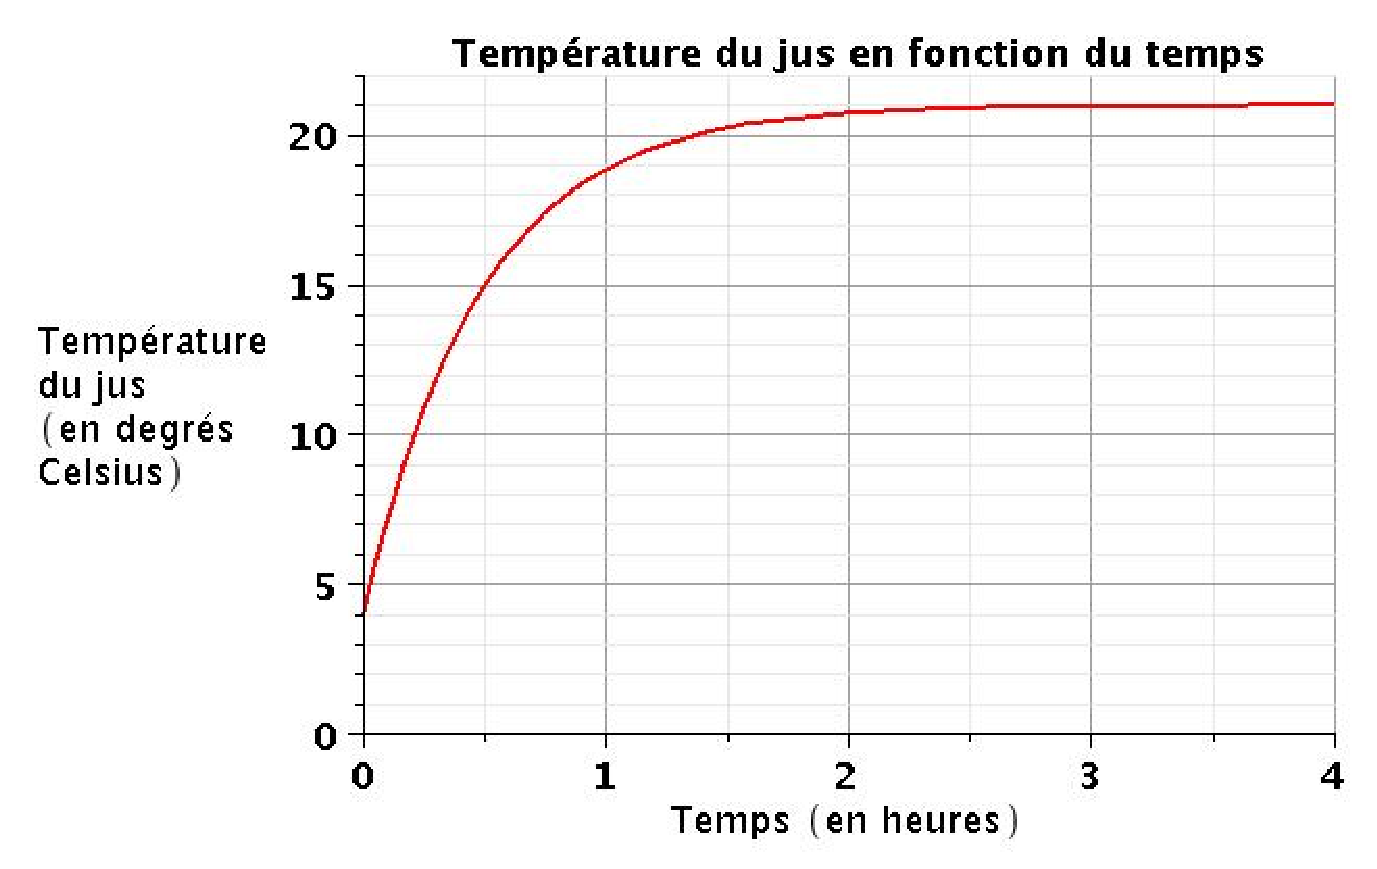
\includegraphics[width=6cm,bb=0 0 400 400]{fonction13.eps}
% fonction13.eps : 300dpi, width=3.39cm, height=3.39cm, bb=0 0 400 400
    \end{center}

C'est une situation de variation nulle.  Par cons\'equent, la r\'eponse est
d).\\

424-- Dans une situation de variation nulle, quelle est la variation de la
variable d\'ependante?\\
a) Il n'y a pas de variation.\\
b) Variation de 1 entre chaque donn\'ee.\\
c) Variation de 2 entre chaque donn\'ee.\\
d) Variation de 4 entre chaque donn\'ee.\\

R\'eponse :  a)\\

R\'etroaction : \\
Voici le graphique d'une fonction de variation nulle.\\
    \begin{center}
    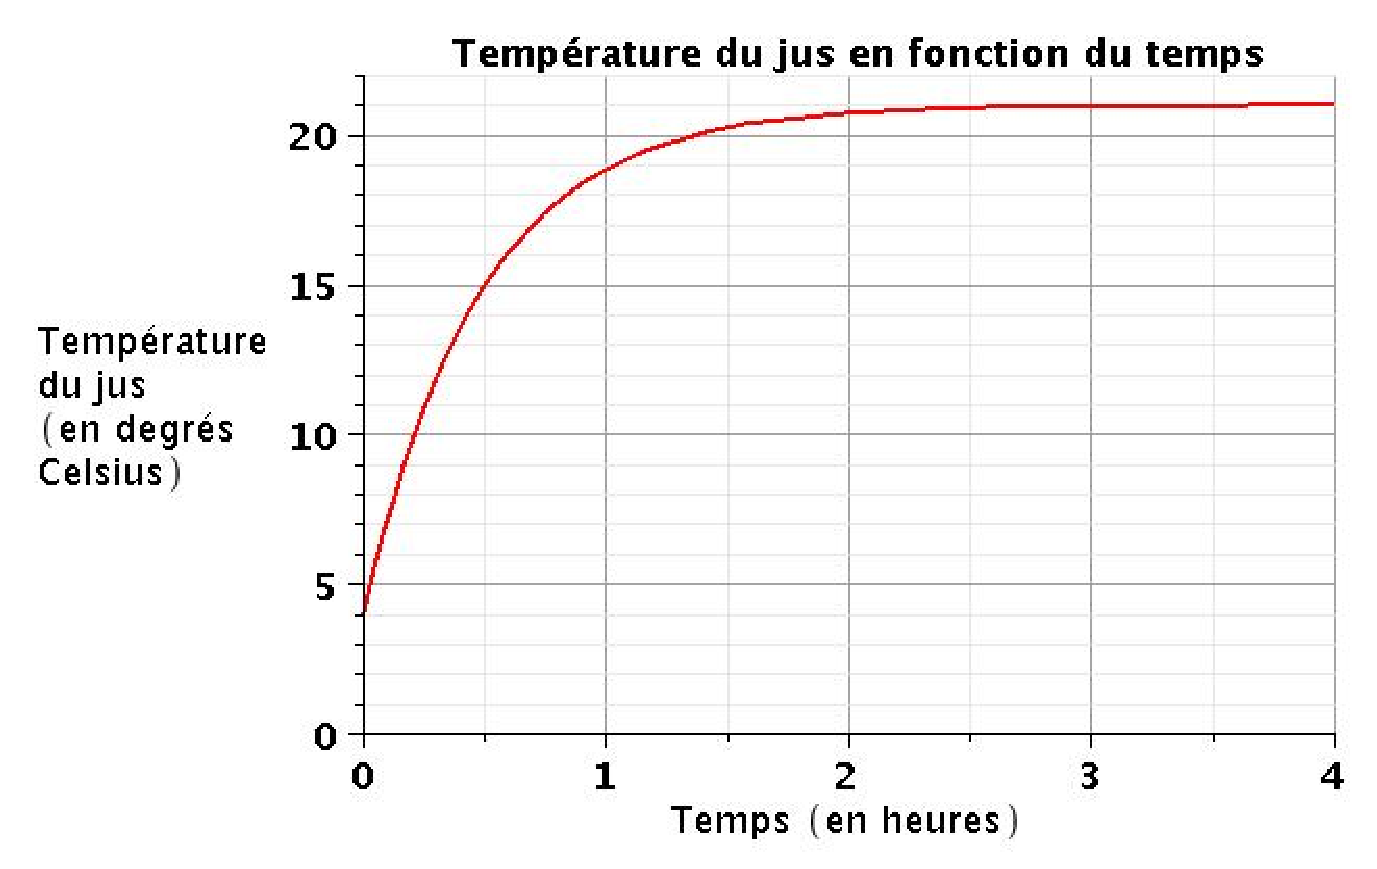
\includegraphics[width=6cm,bb=0 0 400 400]{fonction13.eps}
% fonction13.eps : 300dpi, width=3.39cm, height=3.39cm, bb=0 0 400 400
    \end{center}
La variable d\'ependante est une constante.  Il n'y a donc pas de variation.
  La r\'eponse est a).\\

425-- Parmi les quatre \'enonc\'es suivants, lequel est vrai?\\
a) Dans une situation de variation nulle, il n'y a pas de variable
d\'ependante.\\
b) Dans une situation de variation nulle, la variable d\'ependante est une
constante.\\
c) Dans une situation de variation nulle, la variable d\'ependante varie.\\
d) Dans une situation de variation nulle, la variable ind\'ependante est une
constante.\\


R\'eponse :  b)\\

R\'etroaction : \\
Dans une situation de variation nulle, la variable d\'ependante est une
constante.  Voici le graphique d'une fonction de variation nulle.\\
    \begin{center}
    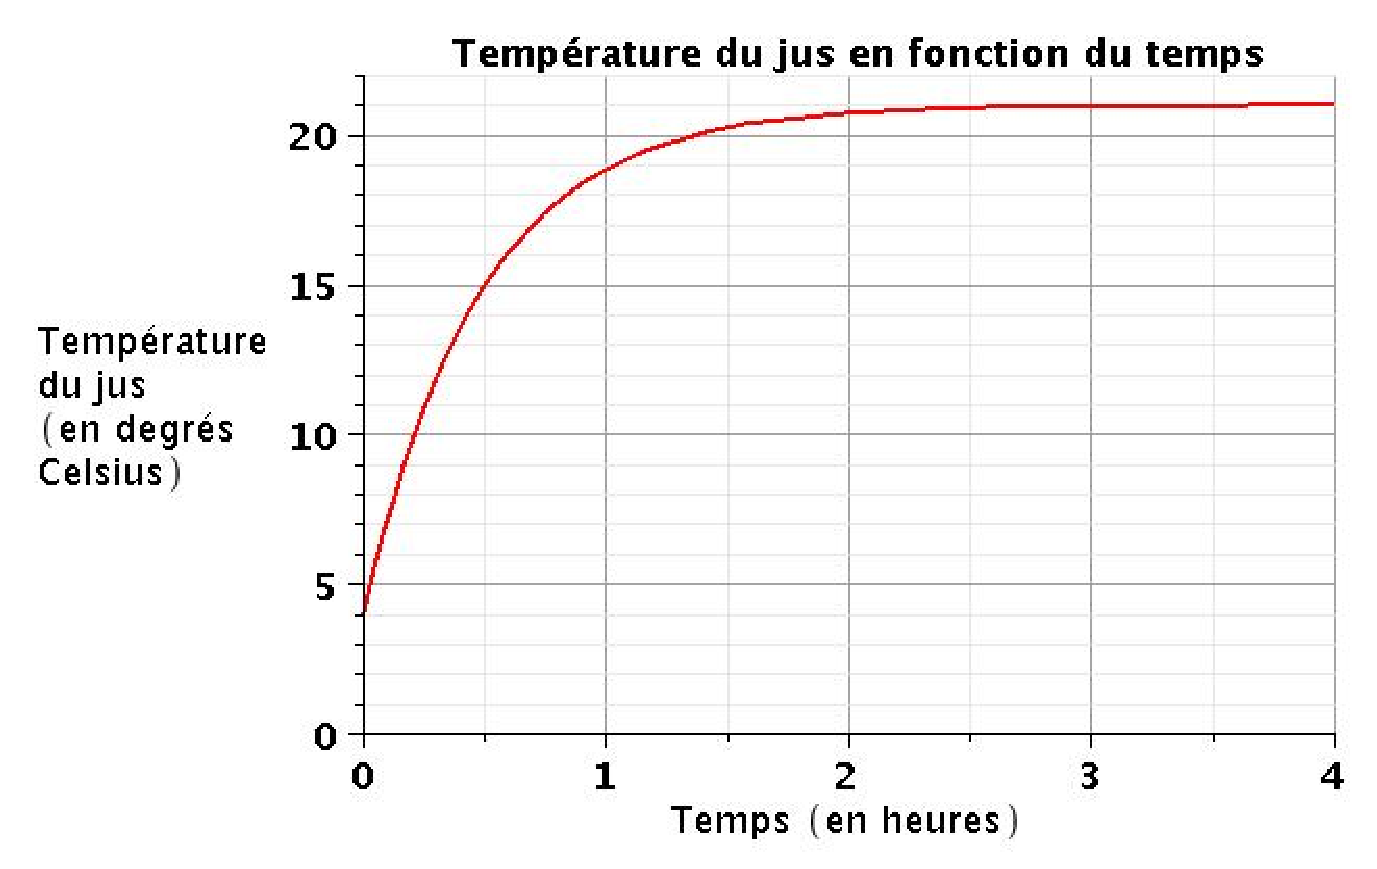
\includegraphics[width=6cm,bb=0 0 400 400]{fonction13.eps}
% fonction13.eps : 300dpi, width=3.39cm, height=3.39cm, bb=0 0 400 400
    \end{center}

La r\'eponse est donc b).\\

426-- Parmi les quatre \'enonc\'es suivants, lequel est vrai?\\
a) Dans une situation de variation nulle, le graphique montre une droite
horizontale.\\
b) Dans une situation de variation nulle, le graphique montre une droite
oblique.\\
c) Dans une situation de variation nulle, le graphique montre une droite
passant absolument par (0, 0).\\
d) Dans une situation de variation nulle, le graphique montre une droite
verticale.\\

R\'eponse :  a)\\

R\'etroaction : \\
Dans une situation de variation nulle, le graphique montre une droite
horizontale.
Voici un exemple d'un tel graphique.\\
    \begin{center}
    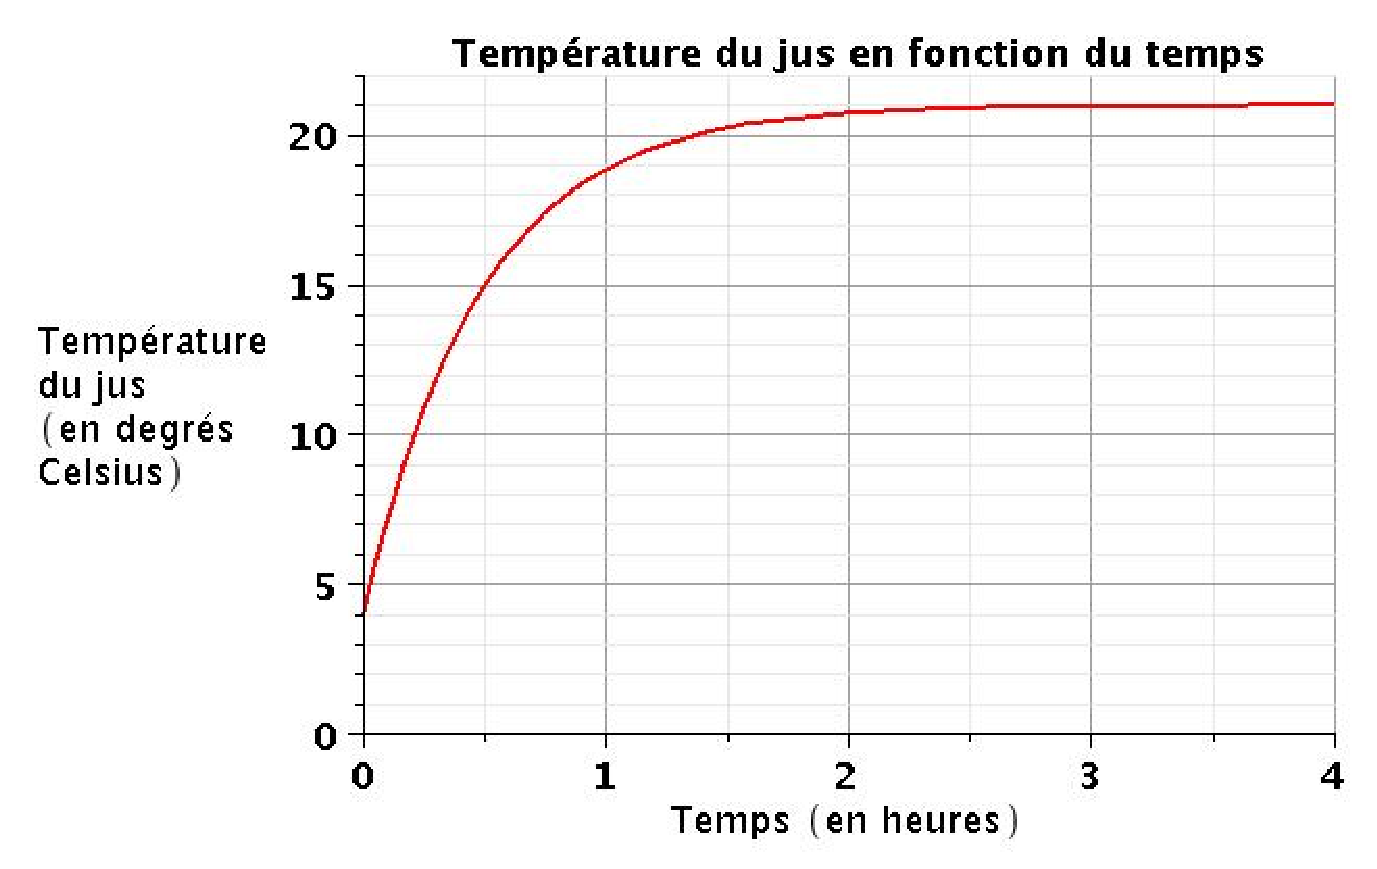
\includegraphics[width=6cm,bb=0 0 400 400]{fonction13.eps}
% fonction13.eps : 300dpi, width=3.39cm, height=3.39cm, bb=0 0 400 400
    \end{center}

La r\'eponse est donc a).\\

427-- Parmi les quatre \'enonc\'es suivants, lequel est vrai?\\
a) Dans une situation de variation directe, le rapport des variations qui se
correspondent est constant.\\
b) Dans une situation de variation directe, le rapport des variations qui se
correspondent n'est pas constant.\\
c) Dans une situation de variation directe, le rapport des variations qui se
correspondent est toujours 1.\\
d) Dans une situation de variation directe, le rapport des variations qui se
correspondent est toujours 2.\\

R\'eponse :  a)\\

R\'etroaction : \\
Dans une situation de variation directe, le rapport des variations qui se
correspondent est constant.
Voici un graphique repr\'esentant une telle situation.\\
    \begin{center}
    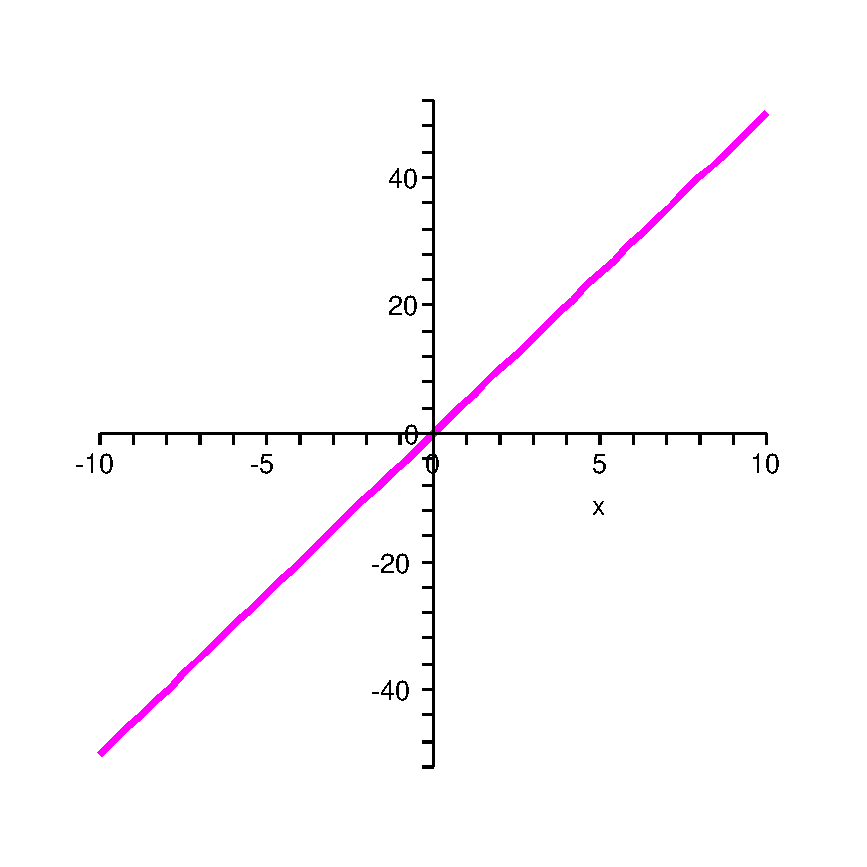
\includegraphics[width=6cm,bb=0 0 400 400]{fonction14.eps}
% fonction14.eps : 300dpi, width=3.39cm, height=3.39cm, bb=0 0 400 400
    \end{center}

La r\'eponse est donc a).\\

428-- Parmi les quatre \'enonc\'es ci-dessous, lequel est vrai?\\
a) Dans une situation de variation directe, le graphique montre une droite
oblique ne passant pas toujours par le point (0, 0).\\
b) Dans une situation de variation directe, le graphique montre une droite
oblique passant toujours par le point (0, 0).\\
c) Dans une situation de variation directe, le graphique montre une droite
oblique ne passant jamais par le point (0, 0).\\
d) Dans une situation de variation directe, le graphique montre une droite
verticale passant par le point (0, 0).\\

R\'eponse :  b)\\

R\'etroaction : \\
Dans une situation de variation directe, le graphique montre une droite
oblique passant toujours par le point (0, 0).  Voici un exemple d'un tel
graphique.\\
    \begin{center}
    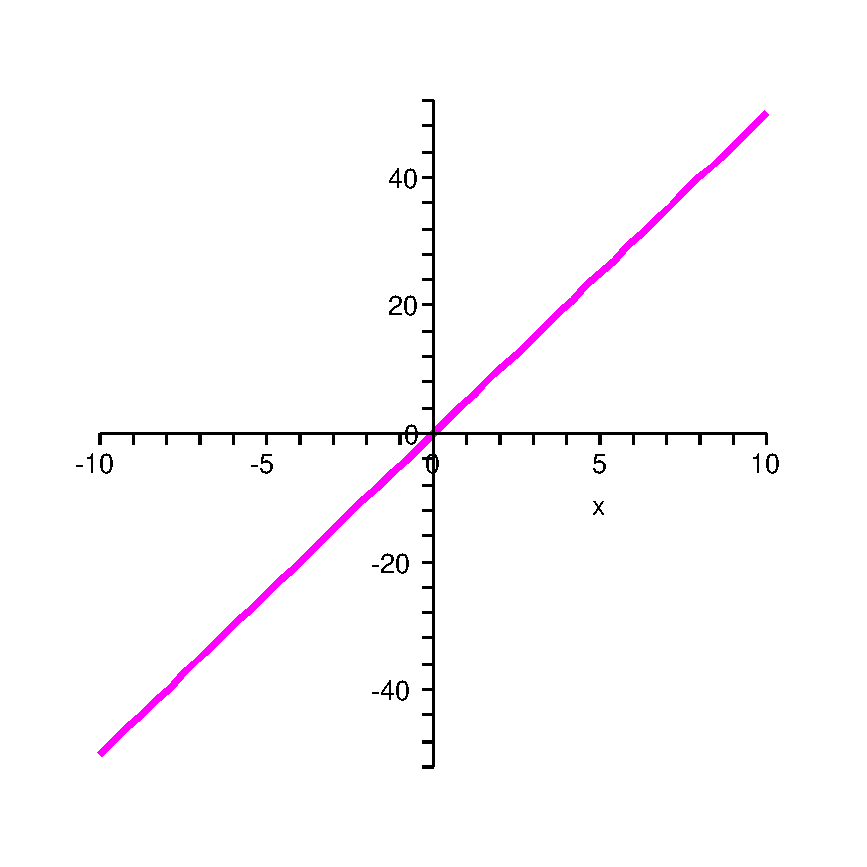
\includegraphics[width=6cm,bb=0 0 400 400]{fonction14.eps}
% fonction14.eps : 300dpi, width=3.39cm, height=3.39cm, bb=0 0 400 400
    \end{center}

La r\'eponse est donc b).\\


429-- Parmi les quatre \'enonc\'es ci-dessous, lequel est vrai?\\
a) Dans une situation de variation partielle, le graphique montre une droite
oblique passant parfois par l'origine du plan et parfois non.\\
b) Dans une situation de variation partielle, le graphique montre une droite
oblique passant par l'origine du plan.\\
c) Dans une situation de variation partielle, le graphique montre une droite
oblique ne passant jamais par l'origine du plan.\\
d) Dans une situation de variation partielle, le graphique montre une droite
ondul\'ee ne passant jamais par l'origine du plan.\\

R\'eponse :  c)\\

R\'etroaction : \\
Dans une situation de variation partielle, le graphique montre une droite
oblique ne passant jamais par l'origine du plan.  Voici un exemple d'un tel
graphique.\\
    \begin{center}
    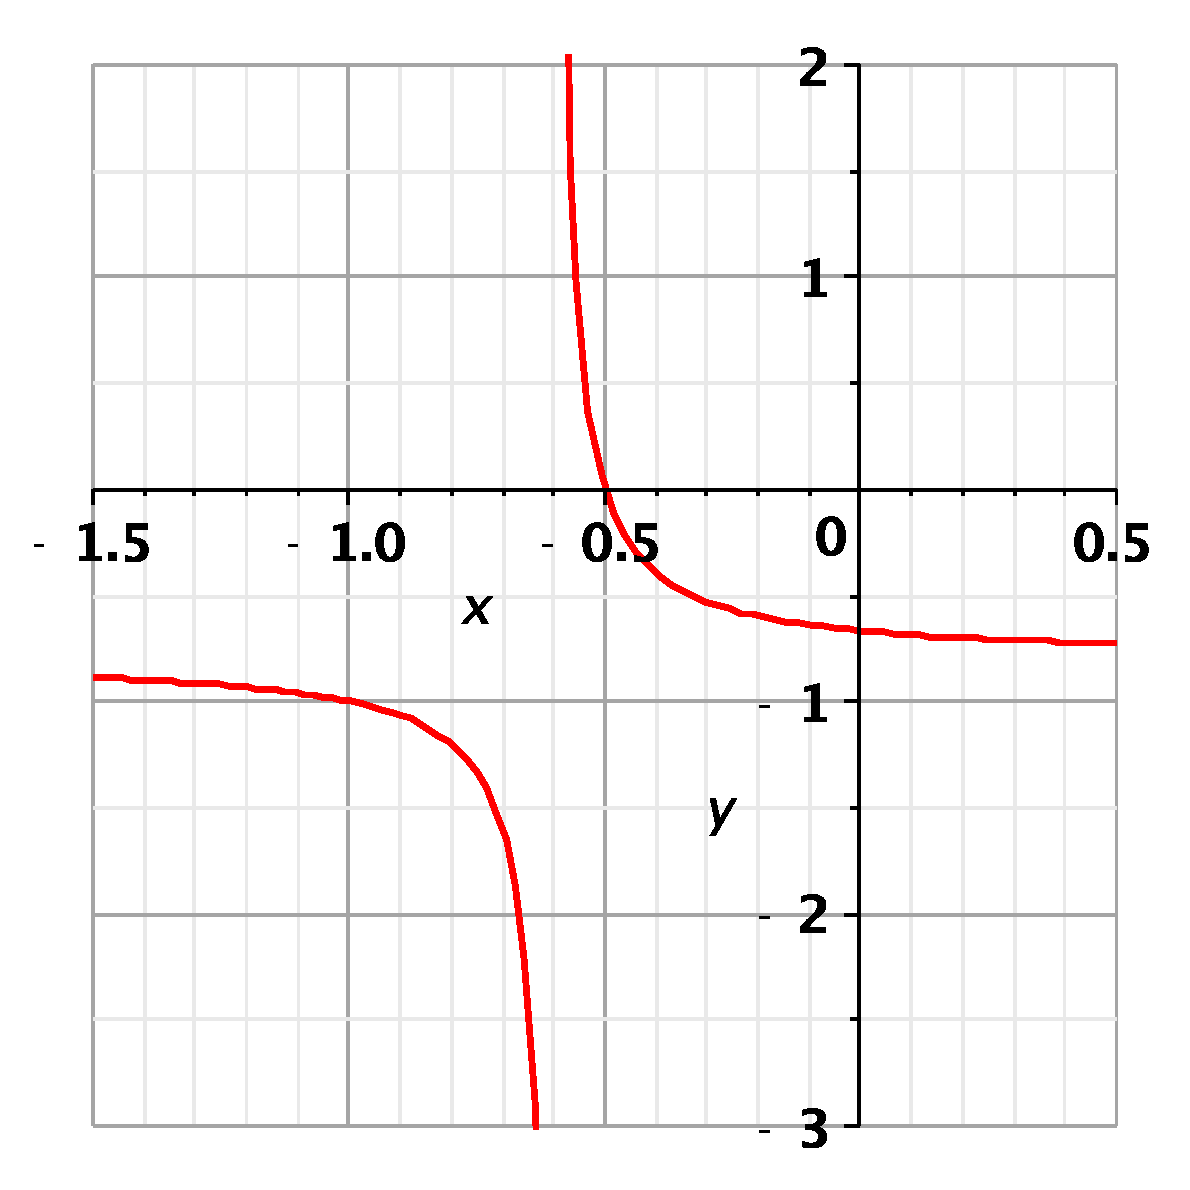
\includegraphics[width=6cm,bb=0 0 400 400]{fonction15.eps}
% fonction15.eps : 300dpi, width=3.39cm, height=3.39cm, bb=0 0 400 400
    \end{center}
La r\'eponse est donc c).\\


430-- Parmi les \'enonc\'es suivants, lequel est vrai?\\
a) Dans une situation de variation inverse, le produit des valeurs reli\'ees
n'est pas constant.\\
b) Dans une situation de variation inverse, le produit des valeurs reli\'ees
est toujours 5.\\
c) Dans une situation de variation inverse, le produit des valeurs reli\'ees
est toujours 10.\\
d) Dans une situation de variation inverse, le produit des valeurs reli\'ees
est constant.\\

R\'eponse :  d)\\

R\'etroaction : \\
Dans une situation de variation inverse, le produit des valeurs reli\'ees
est constant.  Voici un graphique repr\'esentant une telle situation.\\
    \begin{center}
    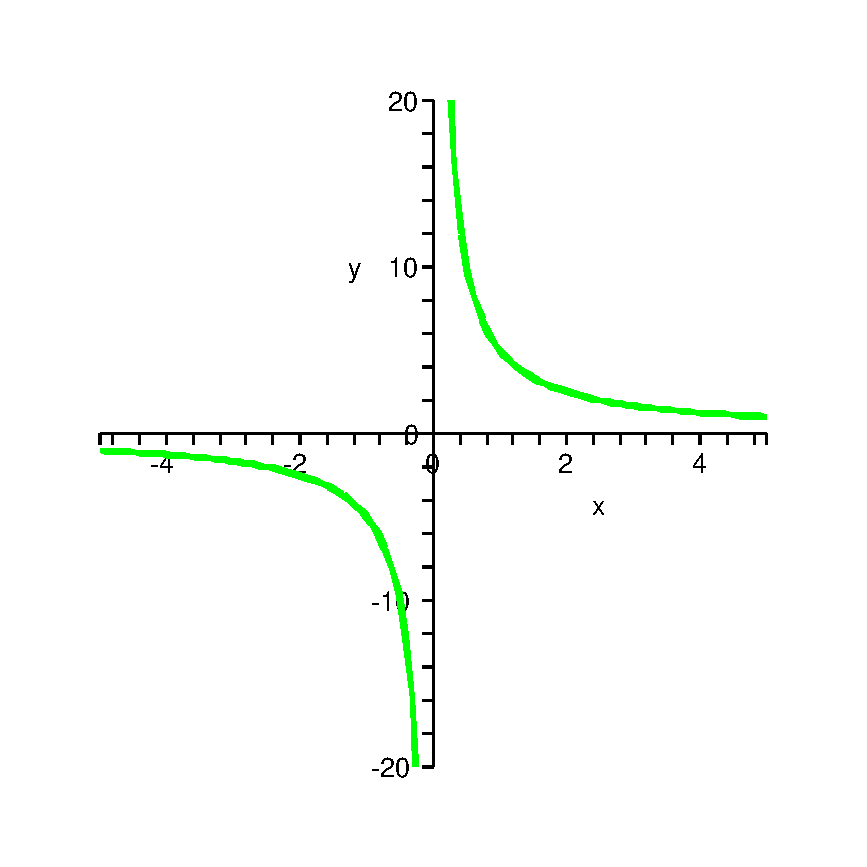
\includegraphics[width=6cm,bb=0 0 400 400]{fonction16.eps}
% fonction16.eps : 300dpi, width=3.39cm, height=3.39cm, bb=0 0 400 400
    \end{center}

Par cons\'equent, la r\'eponse est d).\\




432-- Parmi les quatre \'enonc\'es suivants, lequel est vrai?\\
a) Dans un plan cart\'esien, pour obtenir le taux de variation de la
variable d\'ependante, il faut trouver le quotient de la variation de la
variable d\'ependante sur la variable ind\'ependante.\\
b) Dans un plan cart\'esien, pour obtenir le taux de variation de la
variable d\'ependante, il faut trouver le quotient de la variation de la
variable ind\'ependante sur la variable d\'ependante.\\
c) Dans un plan cart\'esien, pour obtenir le taux de variation de la
variable d\'ependante, il faut trouver le quotient de la variation de la
variable ind\'ependante sur la variable ind\'ependante.\\
d) Dans un plan cart\'esien, pour obtenir le taux de variation de la
variable d\'ependante, il faut trouver le quotient de la variation de la
variable d\'ependante sur la variable d\'ependante.\\

R\'eponse :  a)\\

R\'etroaction : \\
Dans un plan cart\'esien, pour obtenir le taux de variation d'une droite, il
faut trouver le quotient de la variation de la variable d\'ependante sur la
variable ind\'ependante.  La r\'eponse est donc a).\\

433-- Dans un plan cart\'esien, quel est le taux de variation entre deux
points $\left( x_1,y_1\right)$ et $\left( x_2,y_2\right) $?\\
a) $\frac{x_2-x_1}{y_2-y_1}$\\[2mm]
b) $\frac{y_2-y_1}{x_2-x_1}$\\[2mm]
c) $\frac{y_2-x_2}{y_1-x_1}$\\[2mm]
d) $\frac{y_1-x_1}{y_2-x_2}$\\[2mm]

R\'eponse :  b)\\

R\'etroaction : \\
Pour trouver le taux de variation, il faut utiliser
$\frac{y_2-y_1}{x_2-x_1}$.  La r\'eponse est b).\\

434--  Dans un plan cart\'esien, \`a quoi ressemble le graphique d'une
relation de variation partielle?\\
a) Une droite horizontale\\
b) Une droite oblique ne passant pas par l'origine\\
c) Une droite oblique passant par l'origine\\
d) Une droite verticale\\

R\'eponse :  b)\\

R\'etroaction : \\
Dans un plan cart\'esien, le graphique d'une relation de variation partielle
montre une droite oblique ne passant pas par l'origine.  Voici un graphique
repr\'esentant une telle situation.\\
    \begin{center}
    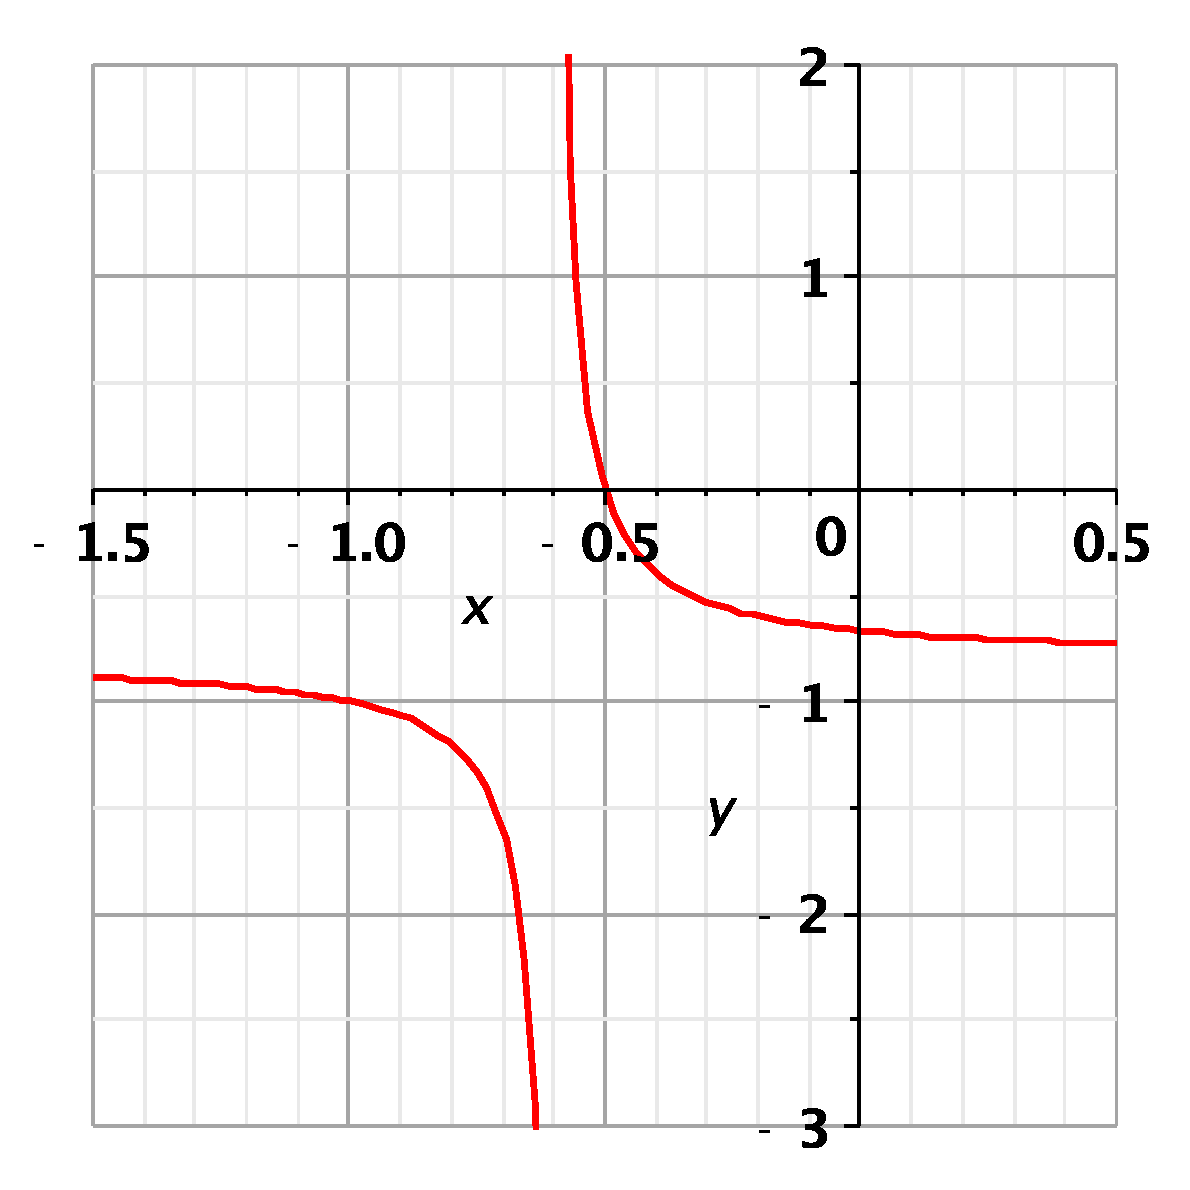
\includegraphics[width=6cm,bb=0 0 400 400]{fonction15.eps}
% fonction15.eps : 300dpi, width=3.39cm, height=3.39cm, bb=0 0 400 400
    \end{center}

La r\'eponse est donc b).\\

435-- Voici l'\'equation d'une droite dans un plan cart\'esien : $y=2x-5$.
Quel est le point d'intersection de cette droite et de l'axe des
ordonn\'ees?\\
a) (0, 2)\\
b) (0, --5)\\
c) (2, 0)\\
d) (--5, 0)\\

R\'eponse :  b)\\

R\'etroaction : \\
Voici le graphique de la fonction $y=2x-5$.\\
    \begin{center}
    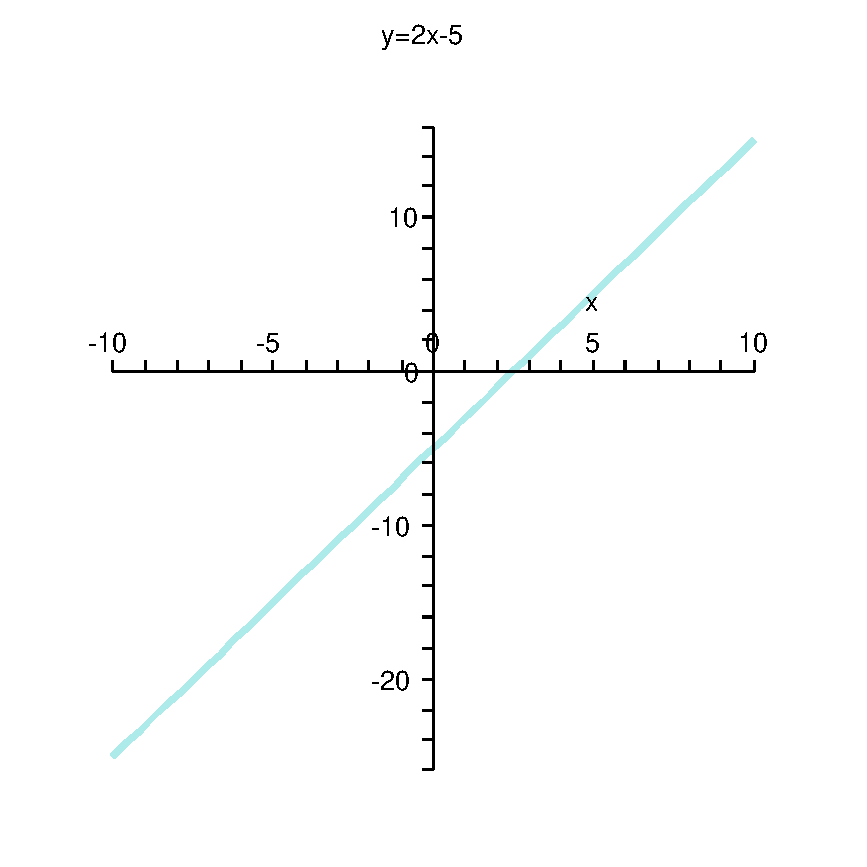
\includegraphics[width=6cm,bb=0 0 400 400]{fonction18.eps}
% fonction18.eps : 300dpi, width=3.39cm, height=3.39cm, bb=0 0 400 400
    \end{center}

La droite $y\,=\,2x\,-\,5$ est de la forme $y\,=\,ax\,+\,b$, o\`u
$a$ donne le taux de variation et $b$ le point d'intersection de la
droite avec l'axe des y, que l'on appelle aussi axe des ordonn\'ees.
Dans le cas pr\'esent, $b\,=\,-5$. Par cons\'equent, la droite coupe
l'axe des ordonn\'ees \`a -5 et le point d'intersection est (0,
--5).
La r\'eponse est donc b).\\

436-- Voici l'\'equation d'une droite dans un plan cart\'esien : $y=2x+10$.
Quel est le point d'intersection de cette droite et de l'axe des
ordonn\'ees?\\
a) (0, 2)\\
b) (0, 10)\\
c) (2, 0)\\
d) (2, 10)\\

R\'eponse :  b)\\

R\'etroaction : \\
Voici le graphique de la fonction $y=2x+10$.\\
    \begin{center}
    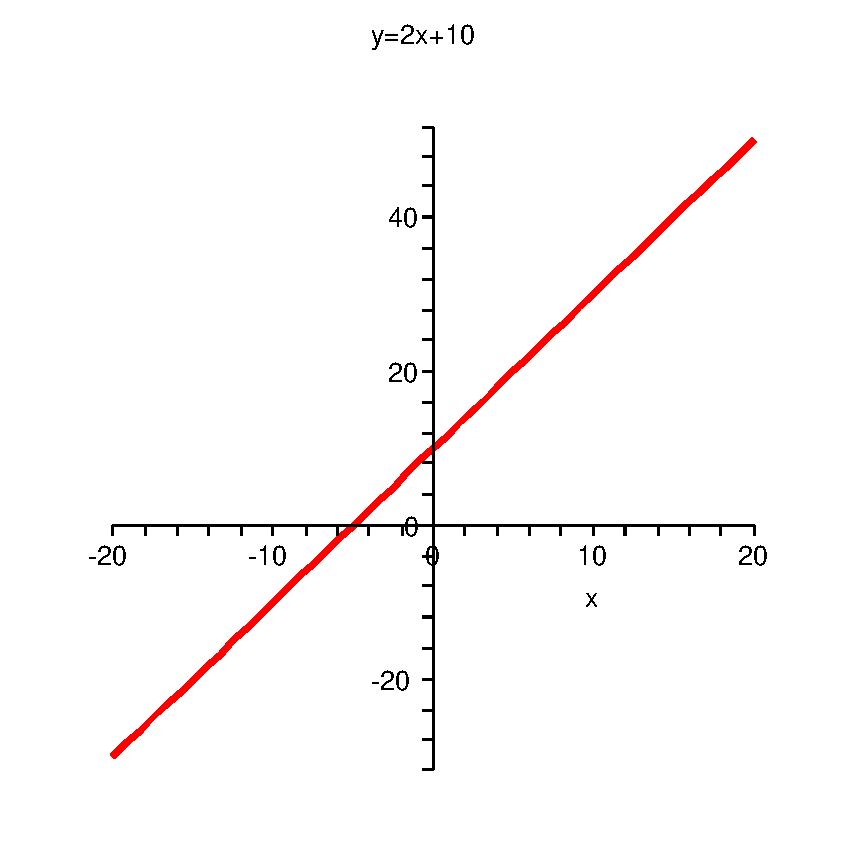
\includegraphics[width=6cm,bb=0 0 400 400]{fonction19.eps}
% fonction19.eps : 300dpi, width=3.39cm, height=3.39cm, bb=0 0 400 400
    \end{center}

La droite $y\,=\,2x\,+\,10$ est de la forme $y\,=\,ax\,+\,b$, o\`u
$a$ donne le taux de variation et $b$ le point d'intersection de la
droite avec l'axe des y, que l'on appelle aussi axe des ordonn\'ees.
Dans le cas pr\'esent, $b\,=\,10$.  Par cons\'equent, la droite
coupe l'axe des ordonn\'ees \`a 10 et le point d'intersection est
(0, 10). La r\'eponse est donc
b).\\

437-- Parmi les quatre choix ci-dessous, lequel repr\'esente l'\'equation
d'une relation de variation partielle dans un plan cart\'esien, o\`u $a$ et
$b$ $\neq0$?\\
a) $y=ax$\\
b) $y=ax+bxy$\\
c) $y=ax+b$\\
d) $y=ax+2bxy$\\


R\'eponse : c)\\

R\'etroaction : \\
Dans un plan cart\'esien, l'\'equation d'une relation de variation partielle
est repr\'esent\'ee par $y=ax+b$, o\`u $a$ est la pente et $b$ est le point
d'intersection avec l'axe des ordonn\'ees.  La r\'eponse est donc c).\\

438-- Dans un plan cart\'esien, l'\'equation d'une droite est donn\'ee par
$y=ax+b$, o\`u $y$ est la variable d\'ependante, $x$ la variable
ind\'ependante, $a$ le taux de variation et $b$ la valeur initiale.
Qu'arrive-t-il \`a la droite si la valeur de $a$ change?\\
a) La droite est r\'efl\'echie par rapport \`a l'axe des abscisses.\\
b) La droite est r\'efl\'echie par rapport \`a l'axe des ordonn\'ees.\\
c) La droite subit une translation verticale.\\
d) La droite pivote autour du point $(0,b)$.\\

R\'eponse : d)\\

R\'etroaction : \\
Si la valeur de $a$ varie, mais que celle de $b$ demeure inchang\'ee, un
seul point reste \`a la m\^eme position et c'est le point $(0,b)$.  La
droite change d'inclinaison et pivote autour de ce point.  Par cons\'equent,
la r\'eponse est d).\\

439-- Dans un plan cart\'esien, l'\'equation d'une droite est donn\'ee par
$y=ax+b$ o\`u $y$ est la variable d\'ependante, $x$ la variable
ind\'ependante, $a$ le taux de variation et $b$ la valeur initiale.
Qu'arrive-t-il \`a la droite si la valeur de $b$ change?\\
a) La droite est r\'efl\'echie par rapport \`a l'axe des abscisses.\\
b) La droite est r\'efl\'echie par rapport \`a l'axe des ordonn\'ees.\\
c) La droite subit une translation verticale.\\
d) La droite pivote autour du point $(0,b)$.\\

R\'eponse : c)\\

R\'etroaction : \\
La pente de la droite restera la m\^eme, mais la droite subira une
translation verticale.  La r\'eponse est donc c).\\

440-- Dans un plan cart\'esien, l'\'equation d'une droite de variation
partielle est donn\'ee par $y=ax+b$, o\`u $y$ est la variable d\'ependante,
$x$ la variable ind\'ependante, $a$ le taux de variation et $b$ la valeur
initiale.  Quel param\`etre de cette \'equation doit-on changer pour obtenir
une relation de variation directe?\\
a) Il faut que $a$ soit \'egal \`a 0.\\
b) Il faut que $a$ soit \'egal \`a 1.\\
c) Il faut que $b$ soit \'egal \`a 0.\\
d) Il faut que $b$ soit \'egal \`a 1.\\

R\'eponse : c)\\

R\'etroaction : \\
Pour obtenir une relation de variation directe, il faut que la droite passe
par l'origine.  Il faut donc que le param\`etre $b$ soit \'egal \`a 0.
Voici un graphique repr\'esentant une telle situation.  \\
    \begin{center}
    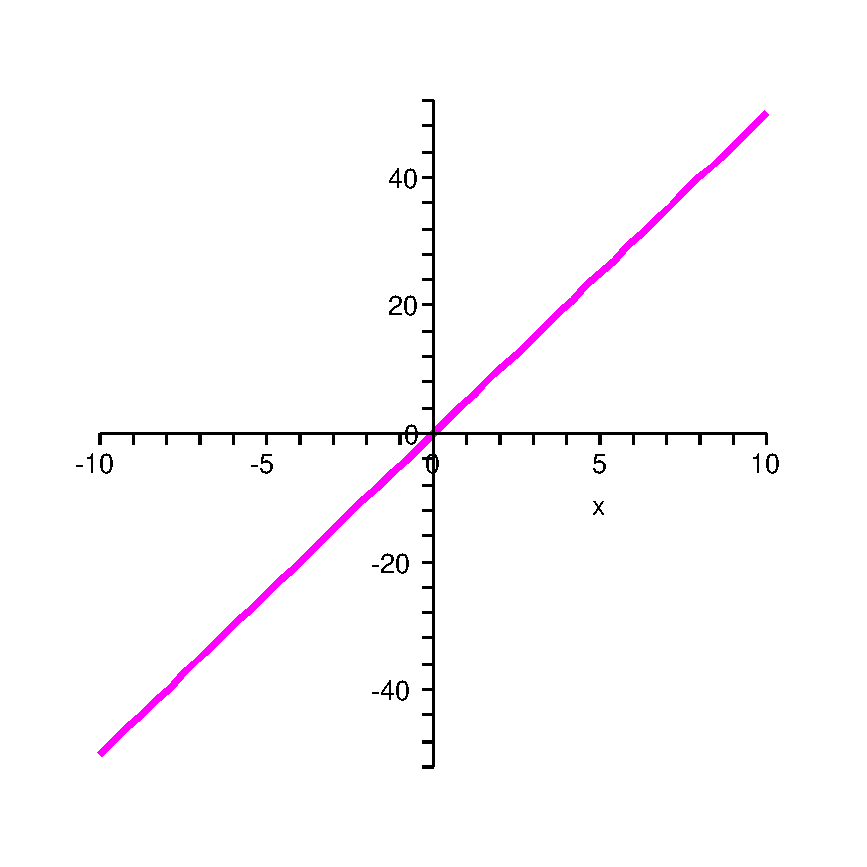
\includegraphics[width=6cm,bb=0 0 400 400]{fonction14.eps}
% fonction14.eps : 300dpi, width=3.39cm, height=3.39cm, bb=0 0 400 400
    \end{center}

La r\'eponse est c).\\


442-- Parmi les quatre objets math\'ematiques ci-dessous, lequel est \`a une
  dimension?\\
a) Une ligne\\
b) Un point\\
c) Un solide\\
d) Une surface\\


R\'eponse : a)\\

R\'etroaction : \\

Un point est un objet math\'ematique n'ayant aucune dimension.\\
Une ligne est un objet math\'ematique \`a une dimension.\\
Une surface est un objet math\'ematique \`a deux dimensions.\\
Un solide est un objet math\'ematique \`a trois dimensions.\\
La r\'eponse est donc a).\\

443-- Parmi les quatre objets math\'ematiques ci-dessous, lequel est \`a
deux dimensions?\\
a) Une ligne\\
b) Un point\\
c) Un solide\\
d) Une surface\\

R\'eponse : d)\\

R\'etroaction : \\
Un point est un objet math\'ematique n'ayant aucune dimension.\\
Une ligne est un objet math\'ematique \`a une dimension.\\
Une surface est un objet math\'ematique \`a deux dimensions.\\
Un solide est un objet math\'ematique \`a trois dimensions.\\
Par cons\'equent, la r\'eponse est d).\\

444-- Parmi les quatre objets math\'ematiques ci-dessous, lequel est \`a
trois dimensions?\\
a) Une ligne\\
b) Un point\\
c) Un solide\\
d) Une surface\\

R\'eponse : c)\\

R\'etroaction : \\
Un point est un objet math\'ematique n'ayant aucune dimension.\\
Une ligne est un objet math\'ematique \`a une dimension.\\
Une surface est un objet math\'ematique \`a deux dimensions.\\
Un solide est un objet math\'ematique \`a trois dimensions.\\
La r\'eponse est donc c).\\

445-- Combien d'ar\^etes un cube poss\`ede-t-il?\\

R\'eponse : 12\\

R\'etroaction : \\
Un cube poss\`ede 12 ar\^etes. Voici l'image d'un cube.\\
    \begin{center}
    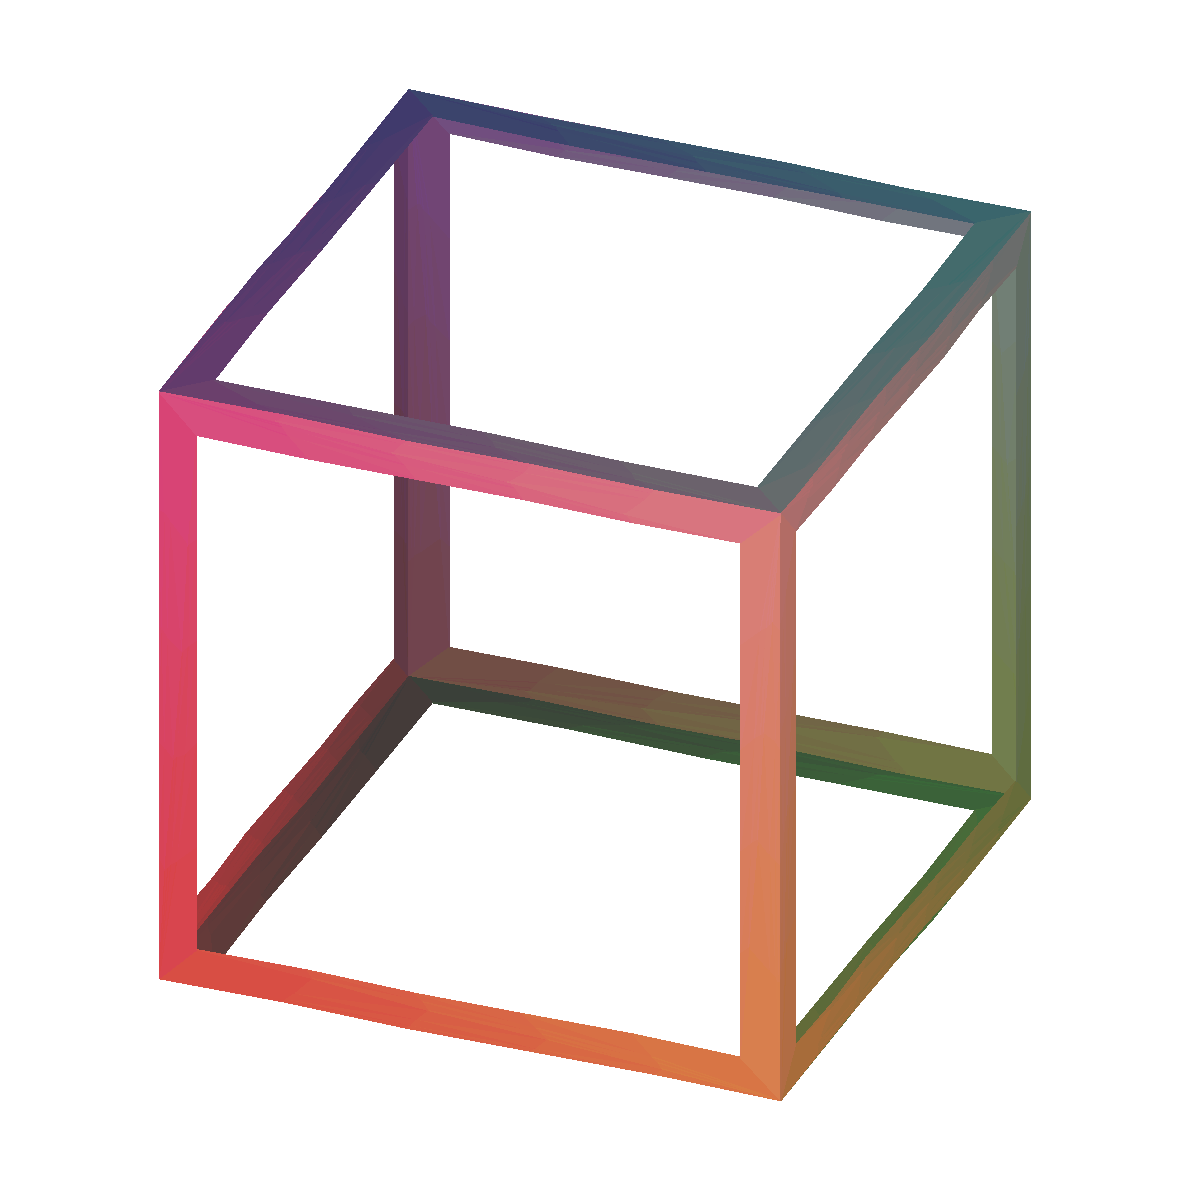
\includegraphics[width=3.8cm]{cube1.eps}
% cube1.eps : 300dpi, width=3.39cm, height=3.39cm, bb=0 0 400 400
    \end{center}



446-- Il n'y a que trois polygones qui permettent de constituer les faces
des poly\`edres convexes r\'eguliers.  Parmi les quatre choix ci-dessous,
lequel \'enum\`ere les trois polygones en question?\\
a) Carr\'e, triangle \'equilat\'eral, hexagone\\
b) Carr\'e, triangle \'equilat\'eral, octogone\\
c) Carr\'e, triangle \'equilat\'eral, pentagone\\
d) Carr\'e, triangle \'equilat\'eral, rectangle\\


R\'eponse : c)\\

R\'etroaction : \\
Les trois polygones r\'eguliers permettant de construire les poly\`edres
convexes r\'eguliers sont le carr\'e, le triangle \'equilat\'eral et le
pentagone.  La r\'eponse est donc c).\\

447-- Combien de poly\`edres convexes r\'eguliers existe-t-il?\\

R\'eponse : 5\\

R\'etroaction : \\
Il existe une infinit\'e de polygones convexes r\'eguliers.  Par contre, il
n'existe que cinq poly\`edres convexes r\'eguliers.  Ce sont le
t\'etra\`edre, le cube, le dod\'eca\`edre, l'octa\`edre et l'icosa\`edre.
La r\'eponse est 5.\\
Voici une image d'un dod\'eca\`edre.\\
    \begin{center}
    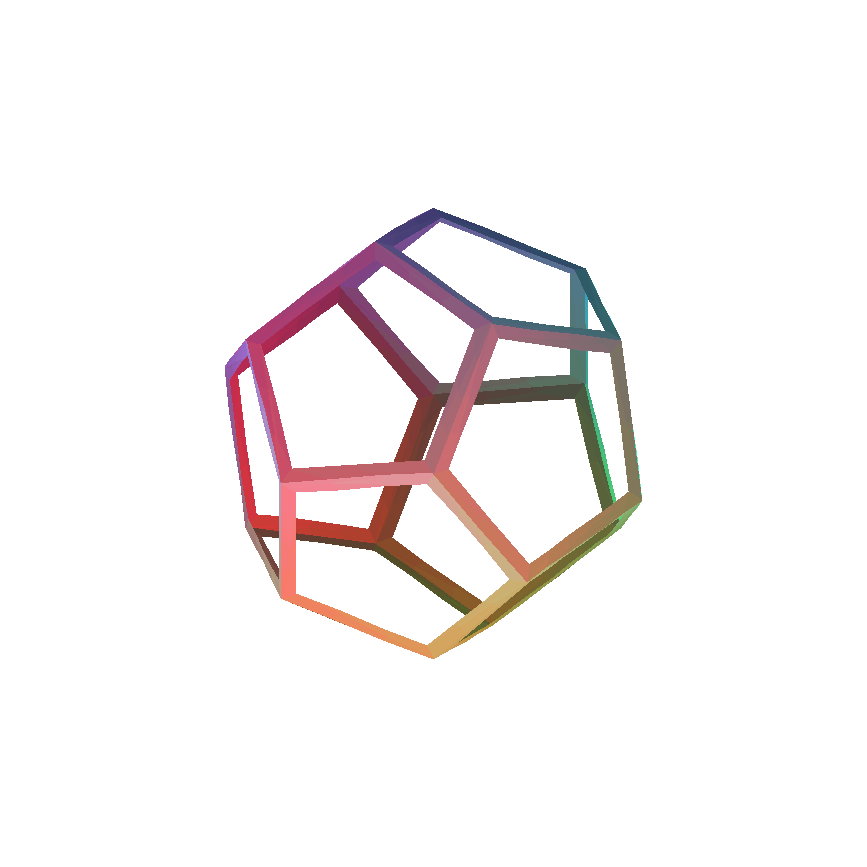
\includegraphics[width=6cm,bb=0 0 400 400]{dodecaedre.eps}
% dodecaedre.eps : 300dpi, width=3.39cm, height=3.39cm, bb=0 0 400 400
    \end{center}
Voici une image d'un cube.\\
    \begin{center}
    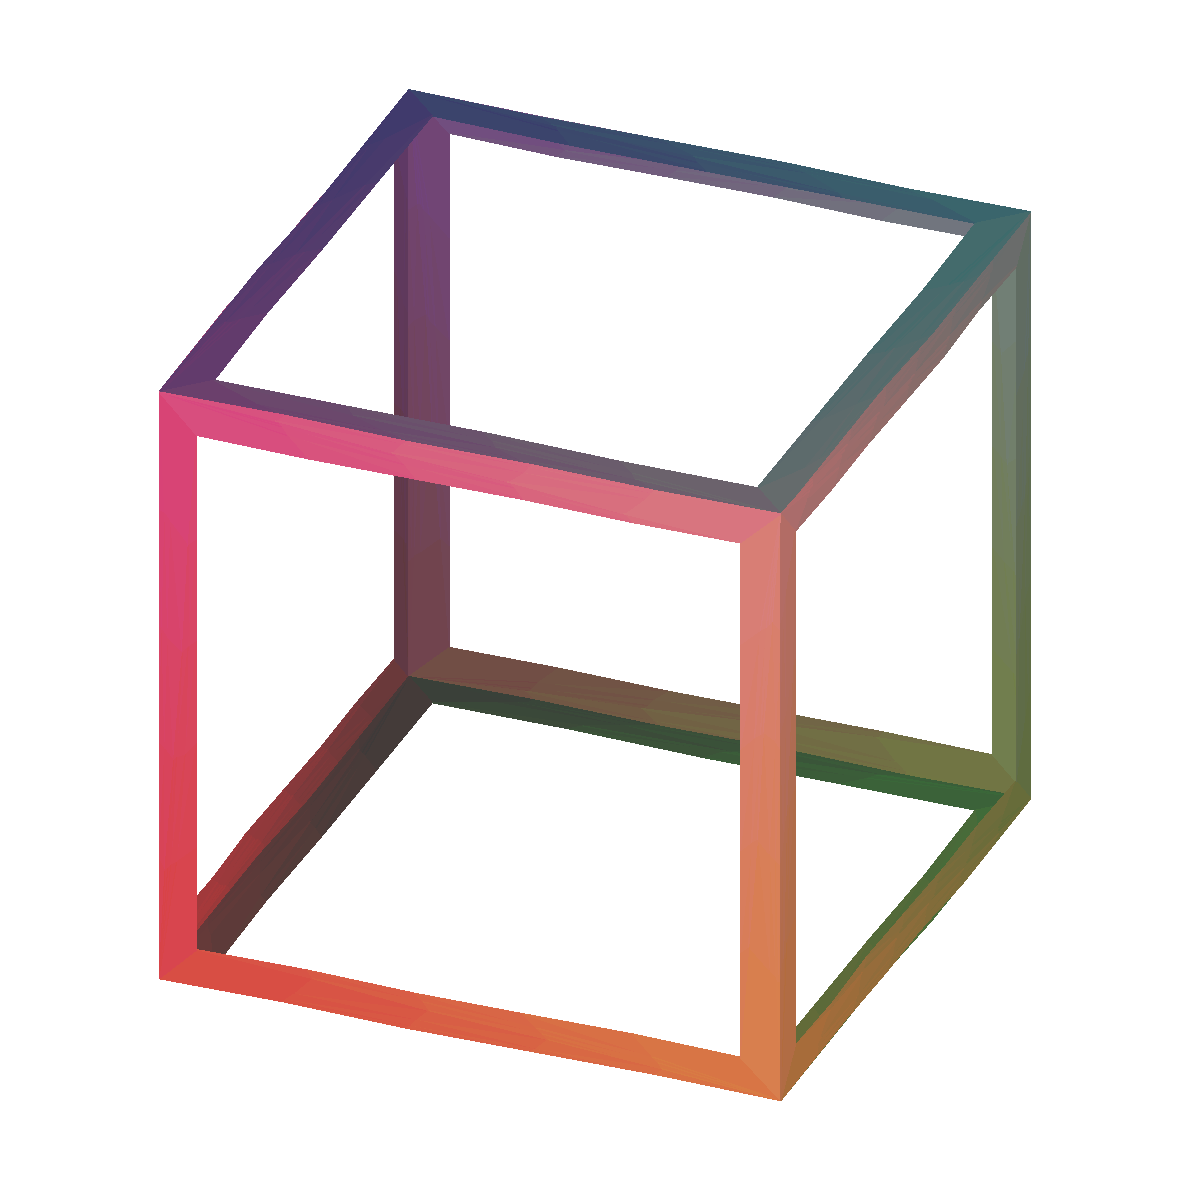
\includegraphics[width=3.8cm]{cube.eps}
% cube.eps : 300dpi, width=3.39cm, height=3.39cm, bb=0 0 400 400
    \end{center}
Voici une image d'un icosa\`edre.\\
    \begin{center}
    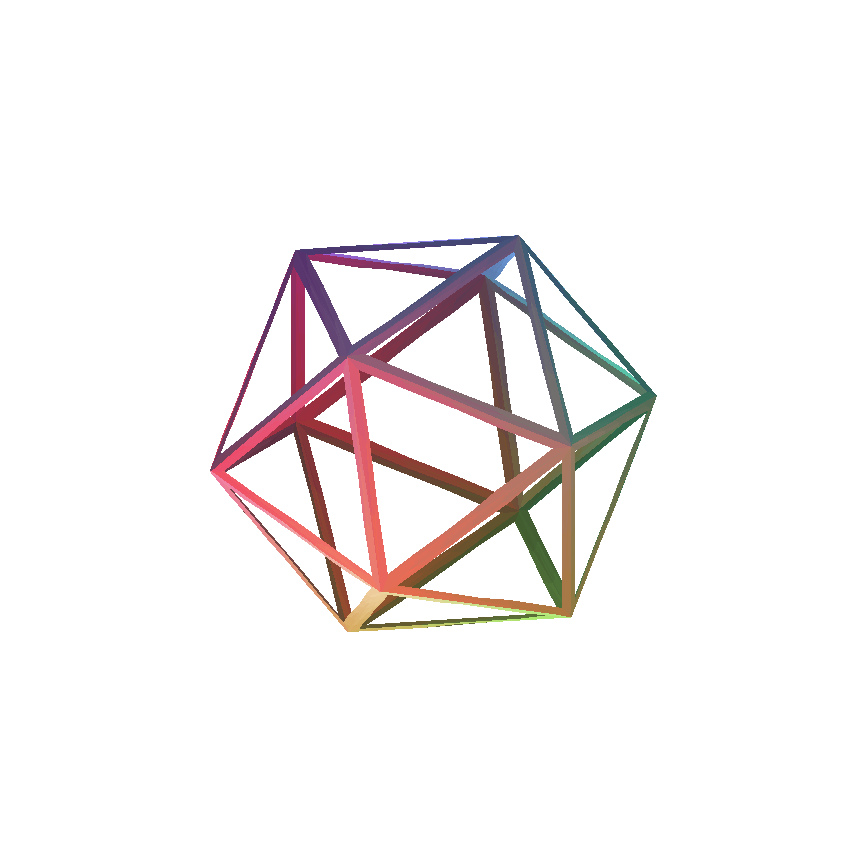
\includegraphics[width=6cm,bb=0 0 400 400]{icosaedre.eps}
% icosaedre.eps : 300dpi, width=3.39cm, height=3.39cm, bb=0 0 400 400
    \end{center}

Voici une image d'un t\'etra\`edre.\\
    \begin{center}
    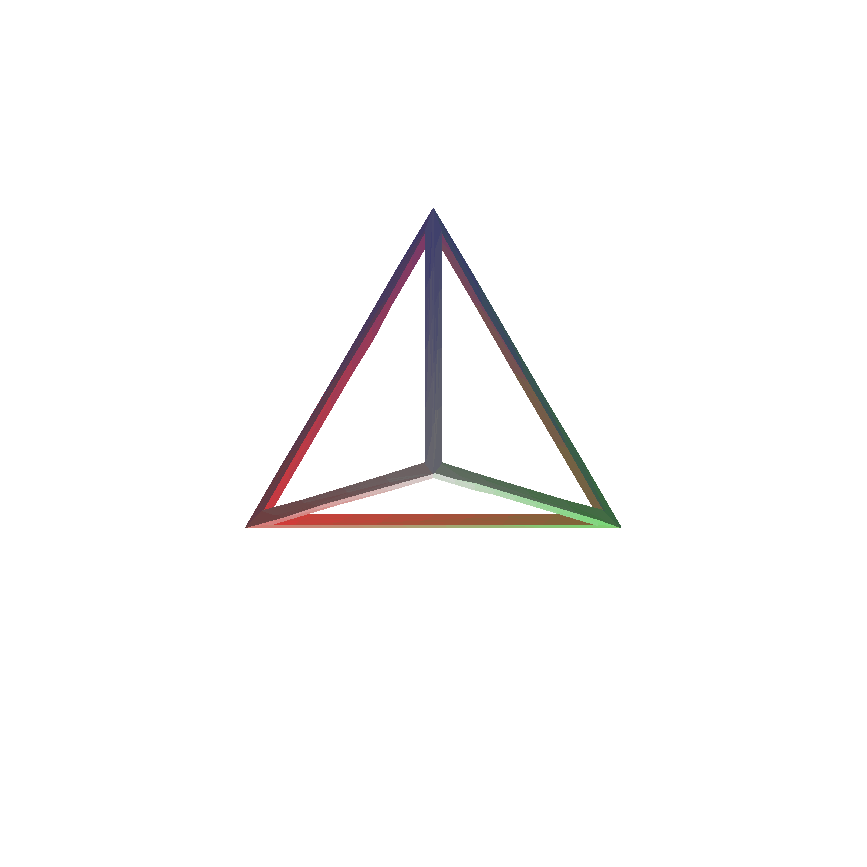
\includegraphics[width=6cm,bb=0 0 400 400]{tetraedre.eps}
% tetraedre.eps : 300dpi, width=3.39cm, height=3.39cm, bb=0 0 400 400
    \end{center}
Voici une image d'un octa\`edre.\\
    \begin{center}
    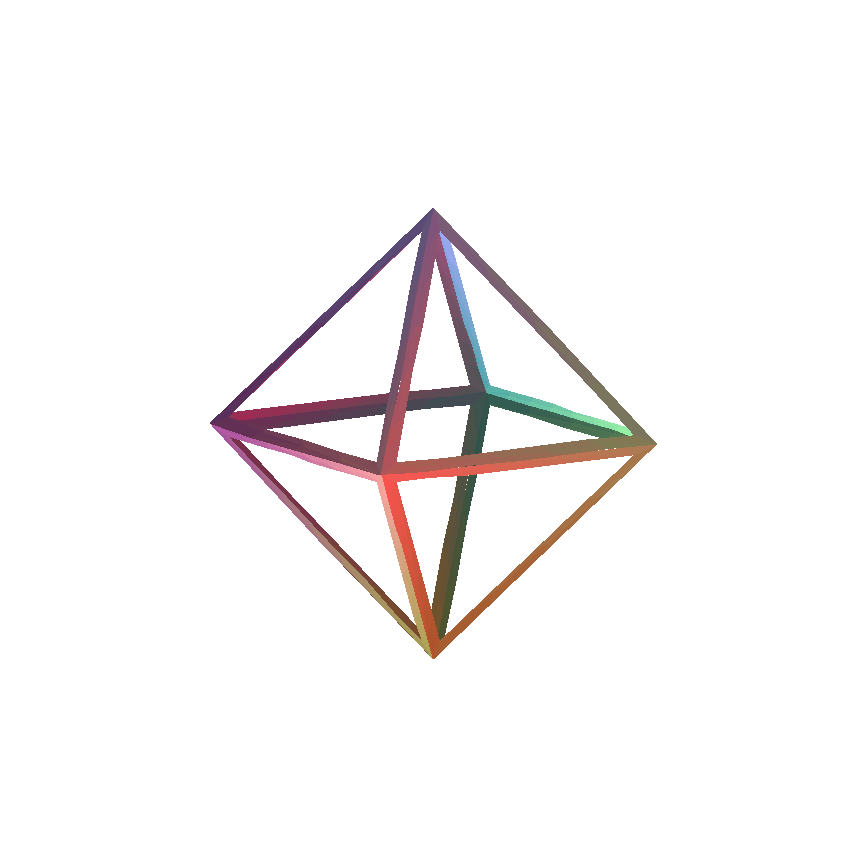
\includegraphics[width=6cm,bb=0 0 400 400]{octaedre2.eps}
% octaedre2.eps : 300dpi, width=3.39cm, height=3.39cm, bb=0 0 400 400
    \end{center}



448--  Combien de faces un t\'etra\`edre poss\`ede-t-il?\\

R\'eponse : 4\\

R\'etroaction : \\
Un t\'etra\`edre est un poly\`edre convexe r\'egulier \`a quatre faces.
Voici l'image d'un t\'etra\`edre.\\
    \begin{center}
    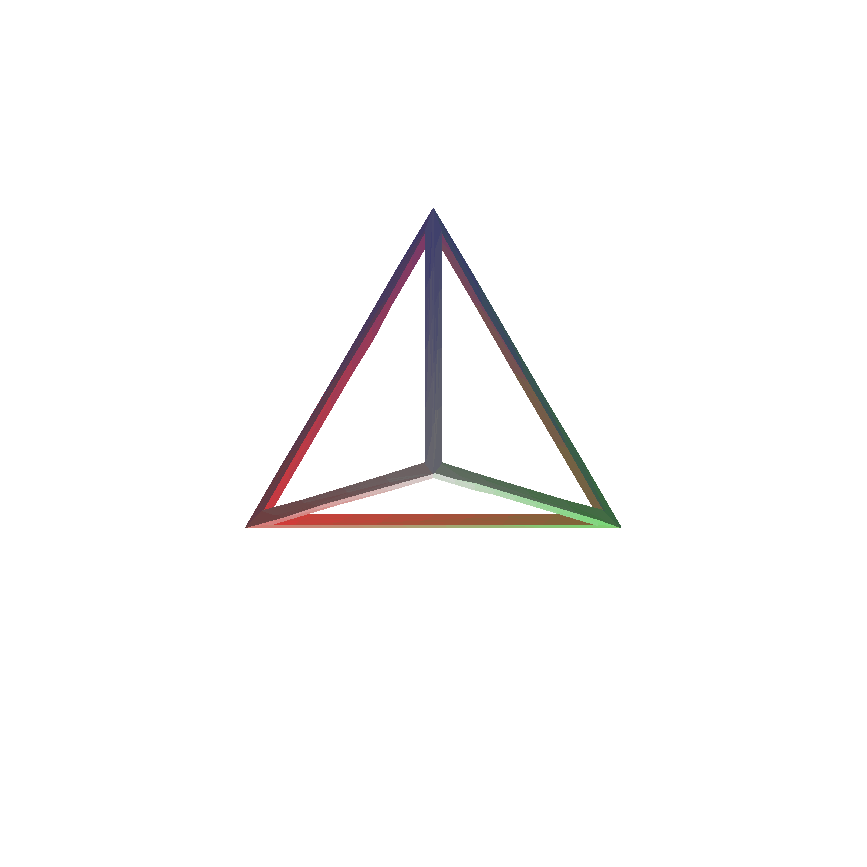
\includegraphics[width=6cm,bb=0 0 400 400]{tetraedre.eps}
% tetraedre.eps : 300dpi, width=3.39cm, height=3.39cm, bb=0 0 400 400
    \end{center}

449--  Combien de faces un dod\'eca\`edre poss\`ede-t-il?\\

R\'eponse : 12\\

R\'etroaction : \\
Un dod\'eca\`edre est un poly\`edre convexe r\'egulier \`a 12 faces.  Voici
l'image d'un dod\'eca\`edre.\\
    \begin{center}
    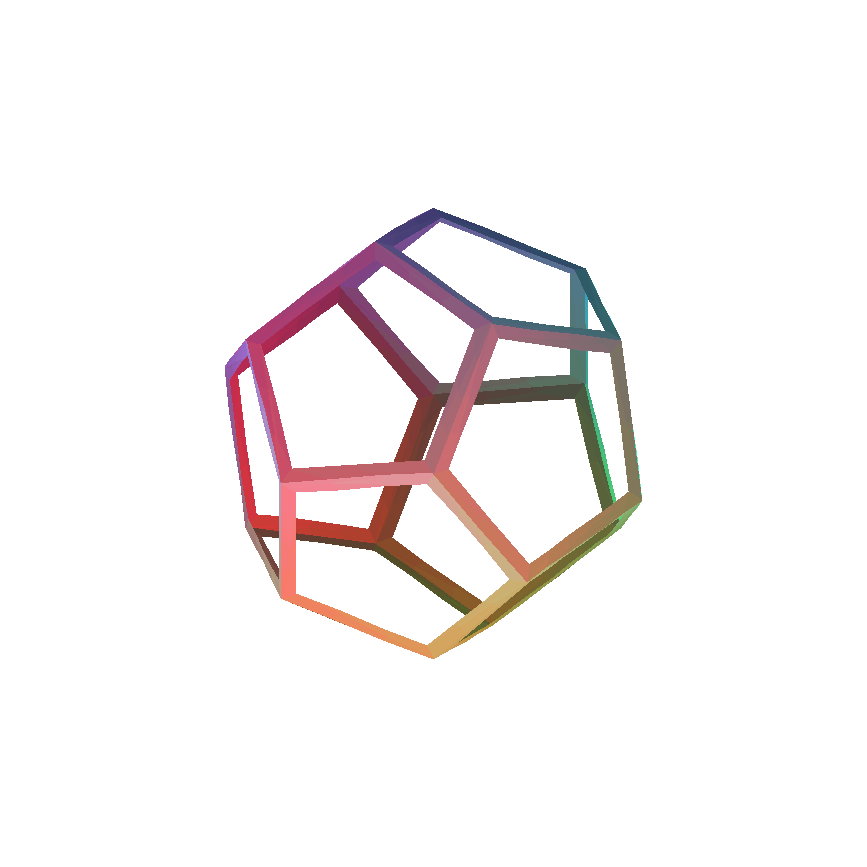
\includegraphics[width=6cm,bb=0 0 400 400]{dodecaedre.eps}
% dodecaedre.eps : 300dpi, width=3.39cm, height=3.39cm, bb=0 0 400 400
    \end{center}


450--  Combien de faces un octa\`edre poss\`ede-t-il?\\

R\'eponse : 8\\

R\'etroaction : \\
Un octa\`edre est un poly\`edre convexe r\'egulier \`a huit faces.  Voici
l'image d'un octa\`edre.\\
    \begin{center}
    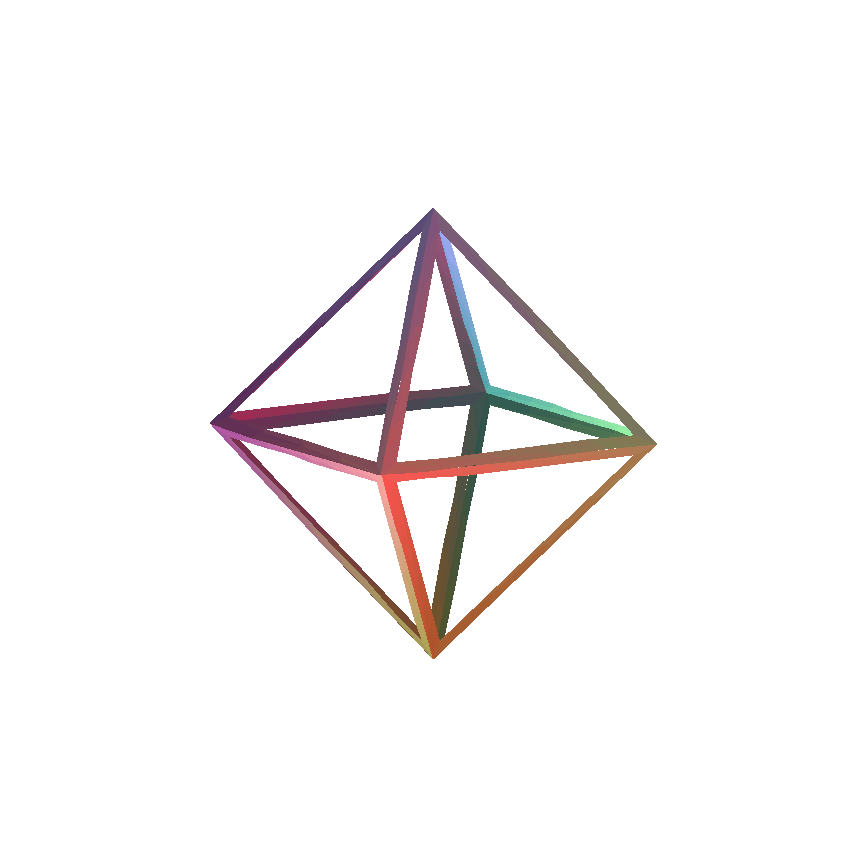
\includegraphics[width=6cm,bb=0 0 400 400]{octaedre2.eps}
% octaedre2.eps : 300dpi, width=3.39cm, height=3.39cm, bb=0 0 400 400
    \end{center}



452-- Combien d'ar\^etes un t\'etra\`edre poss\`ede-t-il?\\

R\'eponse : 6\\

R\'etroaction : \\
Un t\'etra\`edre est un poly\`edre convexe r\'egulier qui poss\`ede six
ar\^etes.  La r\'eponse est donc 6.  Voici l'image d'un t\'etra\`edre.\\
    \begin{center}
    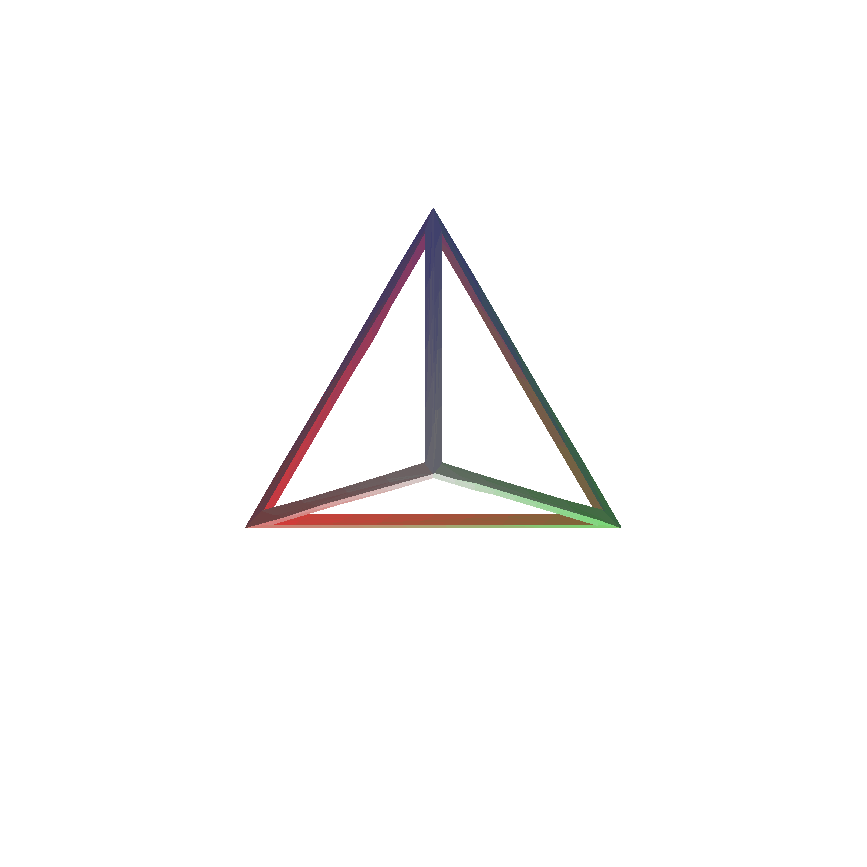
\includegraphics[width=6cm,bb=0 0 400 400]{tetraedre.eps}
% tetraedre.eps : 300dpi, width=3.39cm, height=3.39cm, bb=0 0 400 400
    \end{center}


453--  Le Grand Schtroumpf fait tourner un rectangle de 360$^{\circ}$ autour
d'un axe supportant un de ses c\^ot\'es.  Quel solide g\'en\`ere-t-il?\\
a) C\^one\\
b) Cube\\
c) Cylindre\\
d) Prisme rectangulaire\\


R\'eponse : c)\\

R\'etroaction :\\
Le solide g\'en\'er\'e est un cylindre.  La r\'eponse est c).\\


454--  Le Schtroumpf bricoleur fait tourner un triangle rectangle de
360$^{\circ}$ autour d'un axe supportant un des c\^ot\'es adjacents \`a son
angle droit.  Quel solide g\'en\`ere-t-il?\\
a) C\^one\\
b) Cube\\
c) Cylindre\\
d) Prisme rectangulaire\\

R\'eponse : a)\\

R\'etroaction :\\
Le solide g\'en\'er\'e est un c\^one.  La r\'eponse est a).\\

455-- Parmi les quatre solides ci-dessous, lequel a six sommets, neuf
ar\^etes et cinq faces, dont deux sont des triangles?\\
a) Cylindre triangulaire\\
b) Prisme triangulaire\\
c) Pyramide triangulaire\\
d) T\'etra\`edre\\


R\'eponse : b)\\

R\'etroaction :\\
Seul le prisme triangulaire poss\`ede toutes ces propri\'et\'es.  La
r\'eponse est donc b).\\

456-- Parmi les quatre formules suivantes, laquelle permet de calculer la
surface d'une sph\`ere?\\
a) $\pi r^{2}$\\
b) $2\pi r$\\
c) $\frac{4\pi r^{3}}{3}$\\
d) $4\pi r^{2}$\\

R\'eponse : d)\\

R\'etroaction : \\
Aire d'un disque =  $\pi r^{2}$\\[2mm]
Volume d'une boule = $\frac{4\pi r^{3}}{3}$\\[2mm]
Circonf\'erence d'un cercle = $2\pi r$\\[2mm]
Surface d'une sph\`ere = $4\pi r^{2}$\\[2mm]
Par cons\'equent, la r\'eponse est d).\\

457-- Parmi les quatre formules suivantes, laquelle permet de calculer le
volume d'une boule?\\
a) $\pi r^{2}$\\
b) $2\pi r$\\
c) $\frac{4\pi r^{3}}{3}$\\
d) $4\pi r^{2}$\\

R\'eponse : c)\\

R\'etroaction : \\
Aire d'un disque =  $\pi r^{2}$\\[2mm]
Volume d'une boule = $\frac{4\pi r^{3}}{3}$\\[2mm]
Circonf\'erence d'un cercle = $2\pi r$\\[2mm]
Surface d'une sph\`ere = $4\pi r^{2}$\\[2mm]
La r\'eponse est donc c).\\

458-- Parmi les quatre figures g\'eom\'etriques suivantes, laquelle compose
l'icosa\`edre?\\
a) Carr\'e\\
b) Pentagone\\
c) Rectangle\\
d) Triangle \'equilat\'eral\\

R\'eponse : d)\\

R\'etroaction : \\
Un icosa\`edre est un poly\`edre r\'egulier compos\'e de 20 triangles
\'equilat\'eraux.  Par cons\'equent, la r\'eponse est d).  Voici l'image
d'un icosa\`edre.\\
    \begin{center}
    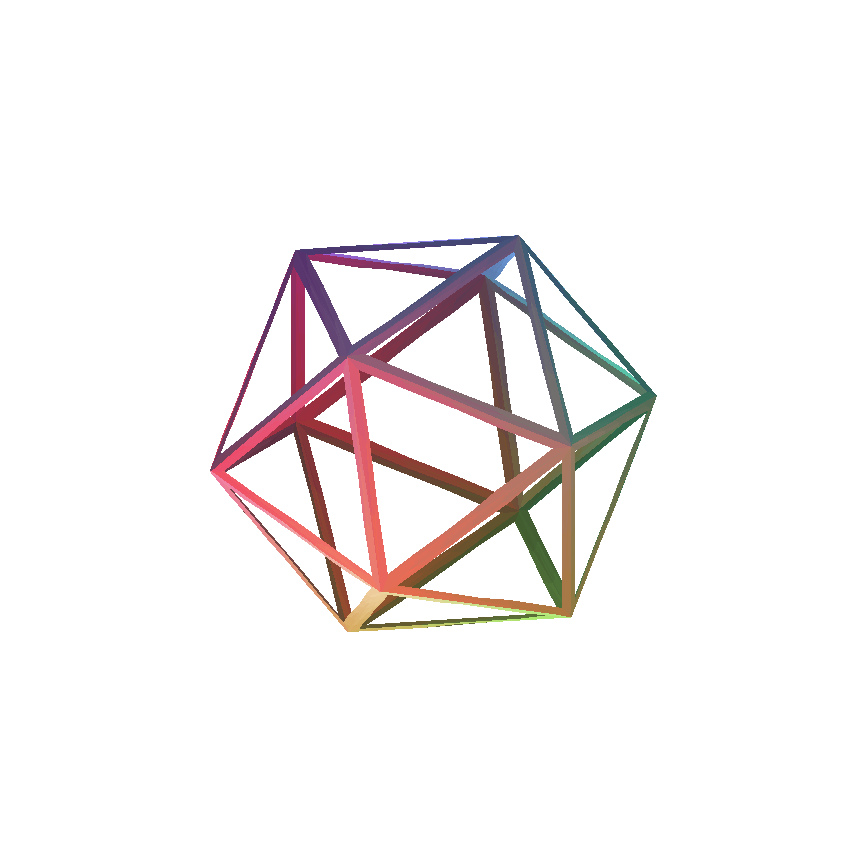
\includegraphics[width=6cm,bb=0 0 400 400]{icosaedre.eps}
% icosaedre.eps : 300dpi, width=3.39cm, height=3.39cm, bb=0 0 400 400
    \end{center}


459-- Parmi les quatre figures g\'eom\'etriques suivantes, laquelle compose
le dod\'eca\`edre?\\
a) Carr\'e\\
b) Pentagone\\
c) Rectangle\\
d) Triangle \'equilat\'eral\\

R\'eponse : b)\\

R\'etroaction : \\
Un dod\'eca\`edre est un poly\`edre r\'egulier compos\'e de 12 pentagones
r\'eguliers.  La r\'eponse est donc b).  Voici l'image d'un
dod\'eca\`edre.\\
    \begin{center}
    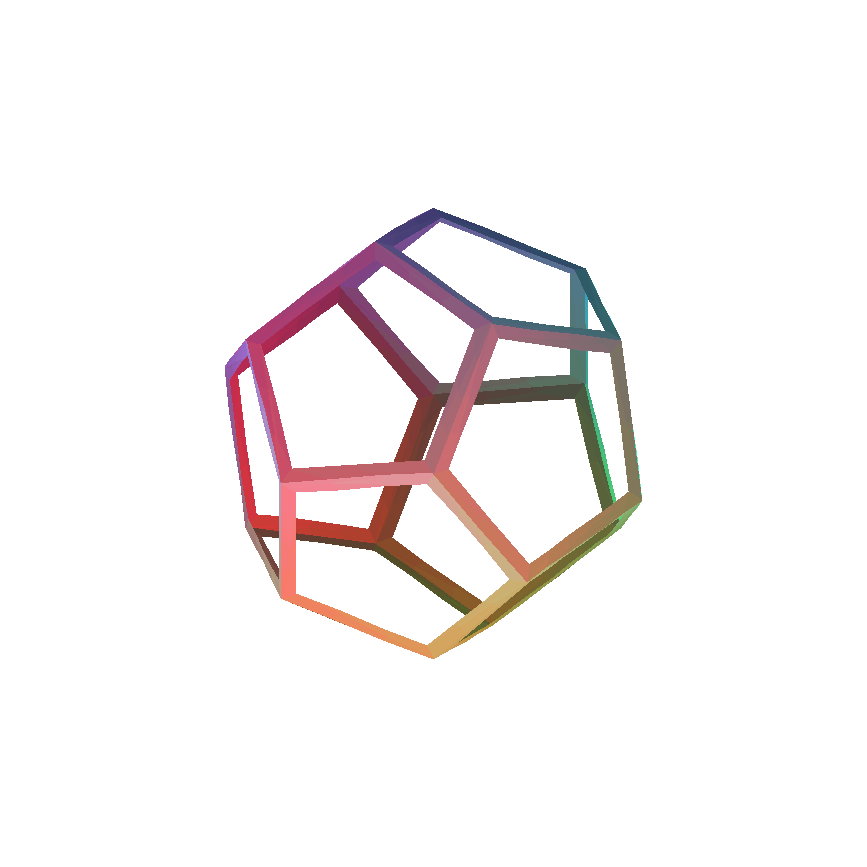
\includegraphics[width=6cm,bb=0 0 400 400]{dodecaedre.eps}
% dodecaedre.eps : 300dpi, width=3.39cm, height=3.39cm, bb=0 0 400 400
    \end{center}


460-- Parmi les quatre figures g\'eom\'etriques suivantes, laquelle compose
l'octa\`edre?\\
a) Carr\'e\\
b) Pentagone\\
c) Rectangle\\
d) Triangle \'equilat\'eral\\

R\'eponse : d)\\

R\'etroaction : \\
Un octa\`edre est un poly\`edre r\'egulier compos\'e de huit triangles
\'equilat\'eraux.  Par cons\'equent, la r\'eponse est d).  Voici l'image
d'un octa\`edre.\\
    \begin{center}
    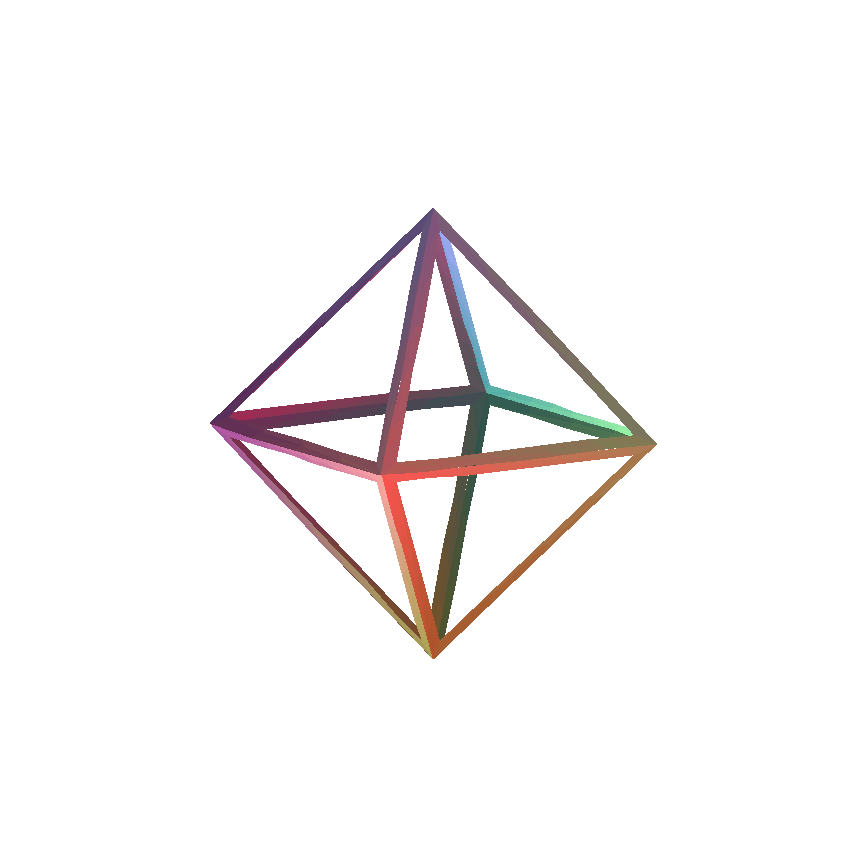
\includegraphics[width=6cm,bb=0 0 400 400]{octaedre2.eps}
% octaedre2.eps : 300dpi, width=3.39cm, height=3.39cm, bb=0 0 400 400
    \end{center}



462-- Un plan coupe un cylindre de telle sorte que la section obtenue est un
rectangle.  Quelle est la position du plan par rapport au cylindre?\\
a) \`A 45$^{\circ}$ par rapport \`a la base\\
b) En angle par rapport \`a la base\\
c) Parall\`ele \`a la base\\
d) Perpendiculaire \`a la base\\

R\'eponse : d)\\

R\'etroaction : \\
Il faut que le plan soit perpendiculaire \`a la base du cylindre
pour obtenir une section rectangulaire.
    \begin{center}
    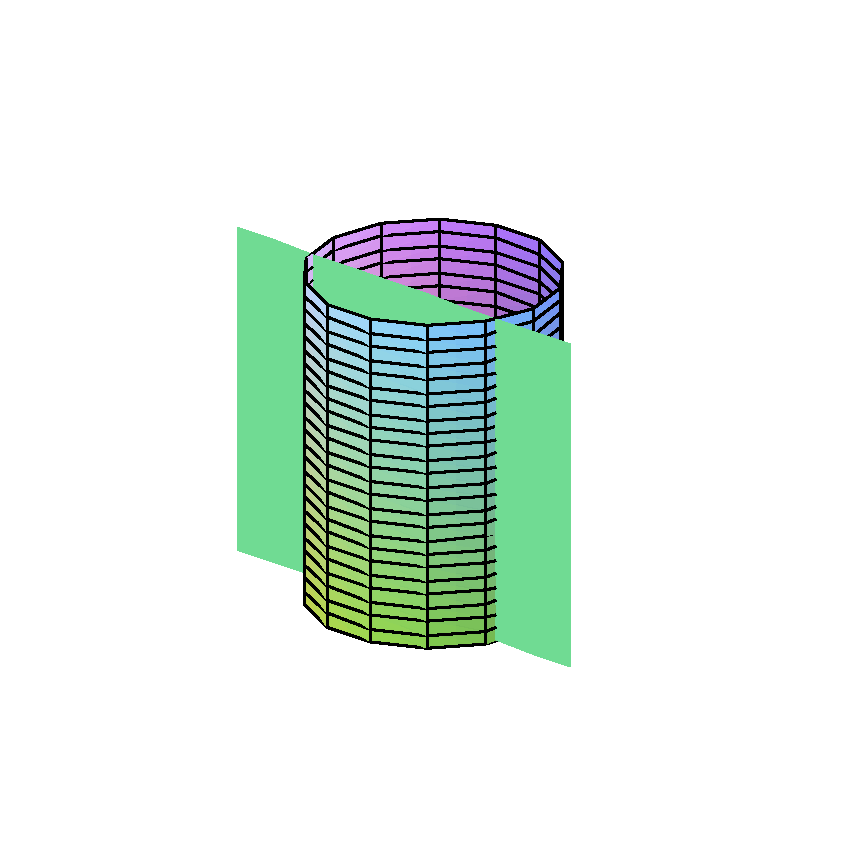
\includegraphics[width=6cm,bb=0 0 400 400]{cylplanvert.eps}
% cylplanvert.eps : 300dpi, width=3.39cm, height=3.39cm, bb=0 0 400 400
    \end{center}

Par cons\'equent, la r\'eponse est d).\\

463-- Un plan coupe un cylindre et la section obtenue est une ellipse.
Quelle est la position du plan par rapport au cylindre?\\
a) Couch\'e par rapport \`a la base\\
b) En angle par rapport \`a la base\\
c) Parall\`ele \`a la base\\
d) Perpendiculaire \`a la base\\

R\'eponse : b)\\

R\'etroaction : \\
Il faut que le plan soit en angle par rapport \`a la base du
cylindre pour obtenir une section en forme d'ellipse.
    \begin{center}
    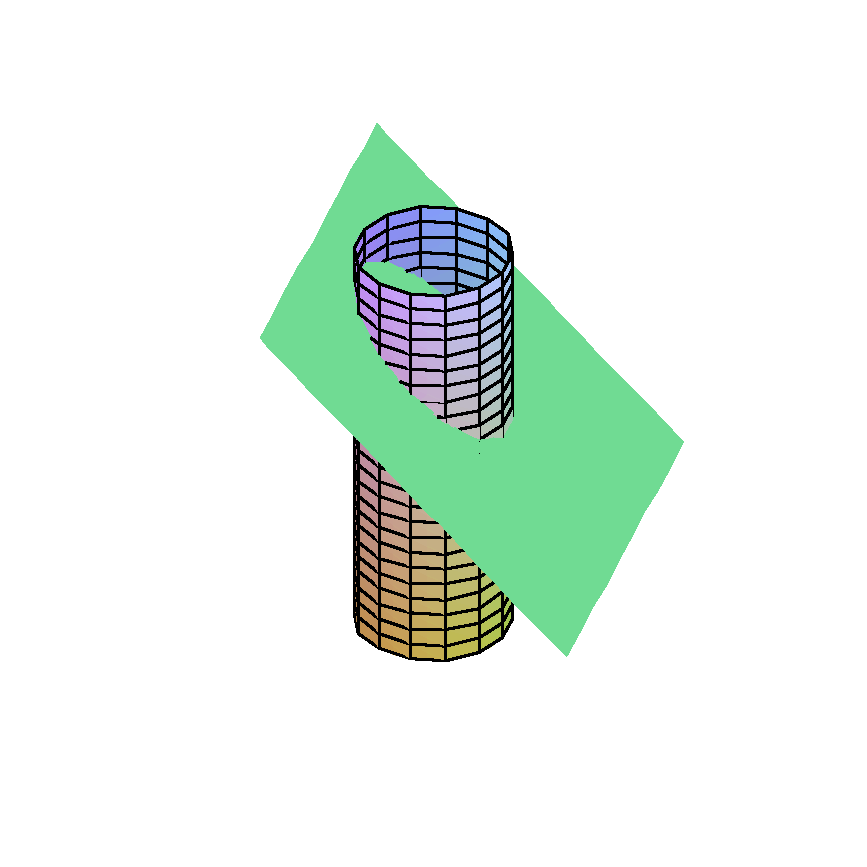
\includegraphics[width=6cm,bb=0 0 400 400]{cylplanobl.eps}
% cylplanobl.eps : 300dpi, width=3.39cm, height=3.39cm, bb=0 0 400 400
    \end{center}

La r\'eponse est donc b).\\


464-- Un plan coupe un c\^one et la section obtenue est un cercle.  Quelle
est la position du plan par rapport au c\^one?\\
a) \`A 45$^{\circ}$ par rapport \`a la base\\
b) En angle par rapport \`a la base\\
c) Parall\`ele \`a la base\\
d) Perpendiculaire \`a la base\\

R\'eponse : c)\\

R\'etroaction : \\
Il faut que le plan soit parall\`ele \`a la base du c\^one pour
obtenir une section circulaire.
    \begin{center}
    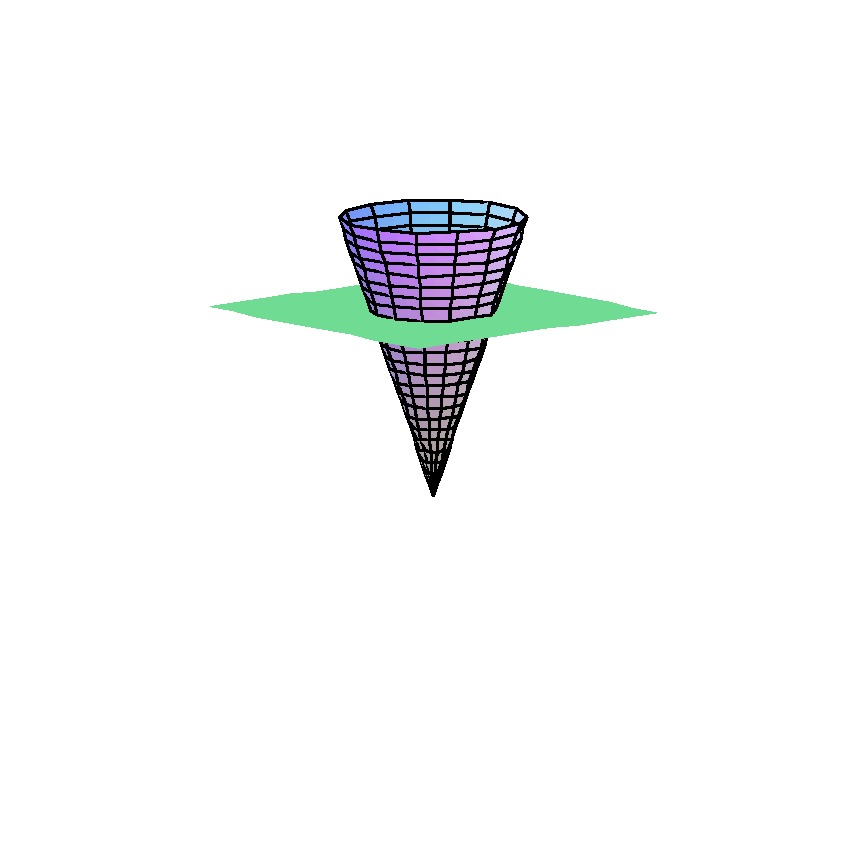
\includegraphics[width=6cm,bb=0 0 400 400]{conplanhor.eps}
% conplanhor.eps : 300dpi, width=3.39cm, height=3.39cm, bb=0 0 400 400
    \end{center}

La r\'eponse est donc c).\\

465-- Un plan coupe un c\^one et la section obtenue est un triangle.  Quelle
est la position du plan par rapport au c\^one?\\
a) \`A 45$^{\circ}$ par rapport \`a la base\\
b) En angle par rapport \`a la base\\
c) Parall\`ele \`a la base\\
d) Perpendiculaire \`a la base\\

R\'eponse : d)\\

R\'etroaction : \\
Il faut que le plan soit perpendiculaire \`a la base du c\^one pour
obtenir une section triangulaire.
    \begin{center}
    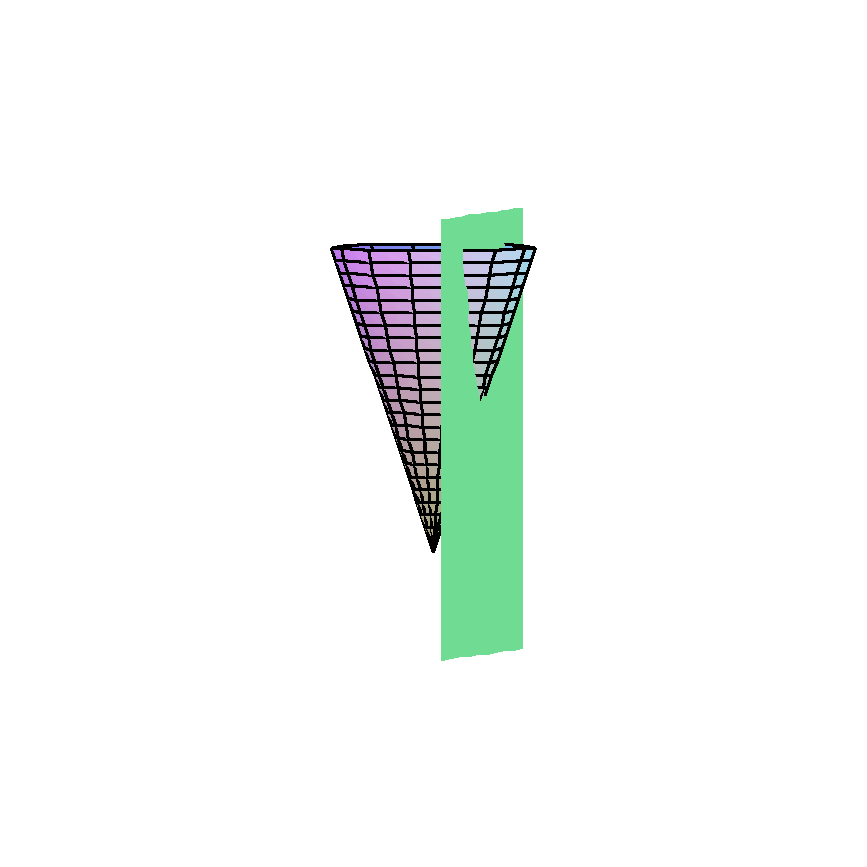
\includegraphics[width=6cm,bb=0 0 400 400]{conplanvert.eps}
% conplanvert.eps : 300dpi, width=3.39cm, height=3.39cm, bb=0 0 400 400
    \end{center}

Par cons\'equent, la r\'eponse est d).\\


466-- Un plan coupe un c\^one et la section obtenue est une ellipse.  Quelle
est la position du plan par rapport au c\^one?\\
a) Couch\'e par rapport \`a la base\\
b) En angle par rapport \`a la base\\
c) Parall\`ele \`a la base\\
d) Perpendiculaire \`a la base\\

R\'eponse : b)\\

R\'etroaction : \\
Il faut que le plan soit en angle par rapport \`a la base du c\^one
pour obtenir une section en forme d'ellipse.
    \begin{center}
    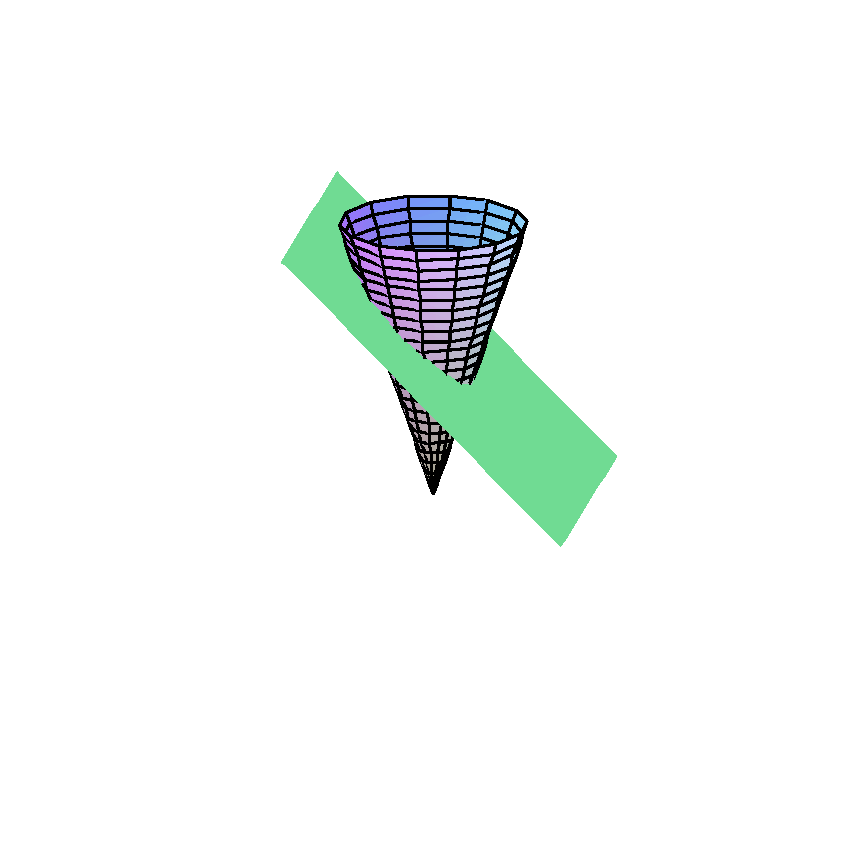
\includegraphics[width=6cm,bb=0 0 400 400]{conplanobl.eps}
% conplanobl.eps : 300dpi, width=3.39cm, height=3.39cm, bb=0 0 400 400
    \end{center}

La r\'eponse est donc b).\\

467-- Un cube est form\'e de 27 petits cubes.  Le grand cube est immerg\'e
en entier dans de la peinture bleue.  Combien y a-t-il de petits cubes
n'ayant aucune face bleue?\\

R\'eponse : 1\\

R\'etroaction : \\
Un seul cube n'a aucune face bleue.  Il s'agit du cube qui est au centre du
grand cube.\\

468-- Un cube est form\'e de 27 petits cubes.  Le grand cube est immerg\'e
en entier dans de la peinture verte.  Combien y a-t-il de petits cubes ayant
exactement 3 faces vertes?\\

R\'eponse : 8\\

R\'etroaction : \\
Il y a huit cubes qui ont exactement trois faces vertes.  Ce sont les
cubes qui forment les huit coins du grand cube. \\

469-- Un cube est form\'e de 27 petits cubes.  Le grand cube est immerg\'e
en entier dans de la peinture rouge.  Combien y a-t-il de petits cubes ayant
exactement une face rouge?\\

R\'eponse : 6\\

R\'etroaction : \\
Il y a six cubes qui ont exactement une face rouge.  Il s'agit des cubes qui
sont au centre de chacune des faces du grand cube.  \\


470-- Un demi-cercle tourne de 360$^{\circ}$ autour d'un axe plac\'e sur son
diam\`etre.  Quel solide est ainsi g\'en\'er\'e?\\
a) C\^one\\
b) Cornet de cr\`eme glac\'ee\\
c) Cylindre\\
d) Sph\`ere\\

R\'eponse : d)\\

R\'etroaction : \\
Le solide obtenu est une sph\`ere.  Par cons\'equent, la r\'eponse est d).\\


472-- Je suis un solide dont la surface n'est pas d\'eveloppable.  Que
suis-je?\\
a) Un c\^one\\
c) Une pyramide\\
b) Un cylindre\\
d) Une sph\`ere\\

R\'eponse : d)\\

R\'etroaction : \\
Il s'agit d'une sph\`ere.
    \begin{center}
    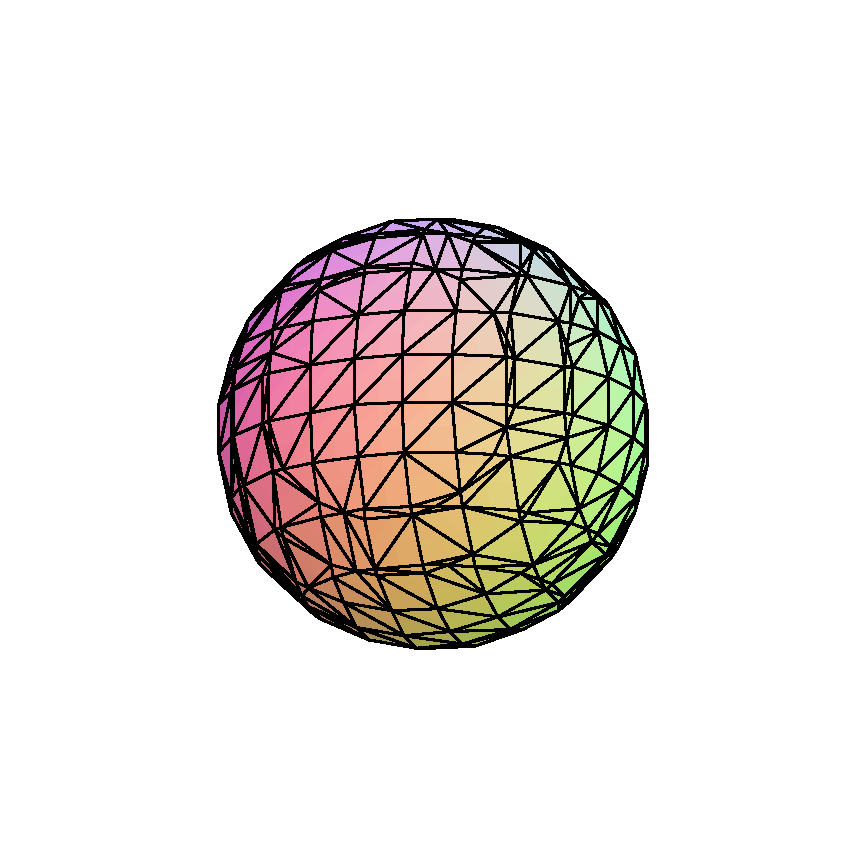
\includegraphics[width=6cm,bb=0 0 400 400]{sphere.eps}
% sphere.eps : 300dpi, width=3.39cm, height=3.39cm, bb=0 0 400 400
    \end{center}

Par cons\'equent, la r\'eponse est d).\\

473-- Combien de sommets un prisme \`a base pentagonal poss\`ede-t-il?\\

R\'eponse : 10\\

R\'etroaction : \\
Un prisme pentagonal a 10 sommets. \\


474-- Dans un triangle rectangle, comment s'appelle le plus long c\^ot\'e?\\
a) Cath\`ete\\
b) Diagonale\\
c) Hypot\'enuse\\
d) Pythagore\\

R\'eponse :  c)\\

R\'etroaction : \\
Le c\^ot\'e le plus long d'un triangle rectangle s'appelle l'hypot\'enuse.
La r\'eponse est donc c).\\


475-- Dans un triangle rectangle, comment s'appellent les deux c\^ot\'es
adjacents \`a l'angle droit?\\
a) Les cath\`etes\\
b) Les hypot\'enuses\\
c) Les petits c\^ot\'es\\
d) Les Pythagores\\

R\'eponse :  a)\\

R\'etroaction : \\
Dans un triangle rectangle, les deux c\^ot\'es adjacents \`a l'angle droit
sont appel\'es les cath\`etes.  La r\'eponse est donc a).\\

476-- Dans un triangle rectangle d'hypot\'enuse de longueur $b$ et de
cath\`etes de longueurs $a$ et $c$, quelle relation peut-on \'etablir \`a
l'aide du th\'eor\`eme de Pythagore?\\
a) $a^{2}+b^{2}=c^{2}$\\
b) $a^{2}\times b^{2}=c^{2}$\\
c) $a^{2}+c^{2}=b^{2}$\\
d) $b^{2}+c^{2}=a^{2}$\\

R\'eponse :  c)\\

R\'etroaction : \\
Dans un triangle rectangle, le carr\'e de l'hypot\'enuse est \'egal \`a la
somme des carr\'es des cath\`etes.  Ici, l'hypot\'enuse est $b$ et les
cath\`etes sont $a$ et $c$.  On obtient la relation
$a^{2}\,+\,c^{2}\,=\,b^{2}$.  La r\'eponse est donc c).\\


477-- Parmi les quatre choix suivants, lequel est un triangle de c\^ot\'es
$a$, $b$ et $c$, o\`u $c$ est le c\^ot\'e le plus long, et v\'erifiant la
relation  $a^{2}+b^{2}=c^{2}$?\\
a) Triangle carr\'e\\
b) Triangle \'equiangle\\
c) Triangle \'equilat\'eral\\
d) Triangle rectangle\\

R\'eponse :  d)\\

R\'etroaction : \\
Un triangle qui v\'erifie la relation $a^{2}+b^{2}=c^{2}$ est un triangle
rectangle. Par cons\'equent, la r\'eponse est d).\\


478-- Le jardin de la Castafiore a la forme d'un triangle rectangle.  Il a
une base de
3 m et une hauteur de 4 m.  Parmi les quatre choix suivants, lequel donne la
longueur du troisi\`eme c\^ot\'e du jardin?\\
a) 3 m\\
b) 4 m\\
c) 5 m\\
d) 5,1416 m\\

R\'eponse :  c)\\

R\'etroaction : \\
En utilisant le th\'eor\`eme de Pythagore, on obtient :\\
$a^{2}+b^{2}=c^{2},\\
3^{2}+4^{2}=c^{2},\\
9+16=c^{2},\\
25=c^{2},\\
c=5$.\\
La r\'eponse est donc c).  Voici la forme du jardin de la Castafiore.\\
    \begin{center}
    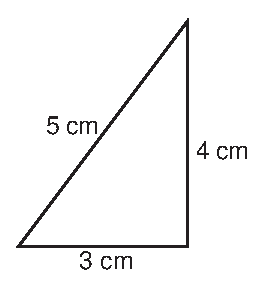
\includegraphics[width=3cm]{triangle22.eps}
% triangle22.eps : 300dpi, width=3.39cm, height=3.39cm, bb=0 0 400 400
    \end{center}


479-- Dans un triangle rectangle, une cath\`ete mesure 4 cm et
l'hypot\'enuse mesure 7 cm.  Quelle est la mesure du troisi\`eme c\^ot\'e?\\
a) $\sqrt{32}$ cm\\
b) $\sqrt{33}$ cm\\
c) $\sqrt{65}$ cm\\
d) $\sqrt{784}$ cm\\

R\'eponse :  b)\\

R\'etroaction : \\
Il faut utiliser le th\'eor\`eme de Pythagore.  \\
$a^{2}+b^{2}=c^{2}\\
4^{2}+b^{2}=7^{2}\\
16+b^{2}=49\\
33=b^{2}\\
\sqrt{33}=b\\$
La r\'eponse est donc b).\\
Voici l'image du triangle rectangle en question.\\
    \begin{center}
    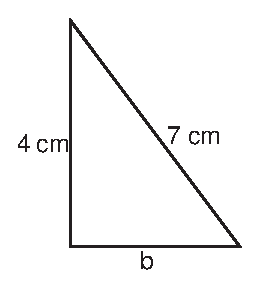
\includegraphics[bb = 0 0 4cm 4cm]{triangle23.eps}
% triangle23.eps : 300dpi, width=3.39cm, height=3.39cm, bb=0 0 400 400
    \end{center}


480--  Une brebis est attach\'ee dans un des quatre coins d'un pr\'e dont
chacun des c\^ot\'es mesure 35 m.  Quelle doit \^etre la longueur de sa
corde pour qu'elle puisse brouter partout?\\
a) 24,75 m\\
b) 40 m\\
c) 49,50 m\\
d) 70 m\\

R\'eponse :  c)\\

R\'etroaction : \\
Il faut utiliser le th\'eor\`eme de Pythagore.  \\
$a^{2}+b^{2}=c^{2}$\\
Comme le pr\'e a la forme d'un carr\'e, $a=b.$\\
$a^{2}+a^{2}=c^{2}\\
2a^{2}=c^{2}\\
2\times35^{2}=c^{2}\\
2\times 1225=c^{2}\\
2450=c^{2}\\
\sqrt{2450}=c\\
c\,=\,49,50$\\
La r\'eponse est donc c).\\


482-- Une aire de jeu a une forme triangulaire.  Les mesures des
c\^ot\'es sont 10 m, 24 m et 26 m.  Parmi les \'enonc\'es suivants,
lequel est vrai?\\
a) Le triangle form\'e a un p\'erim\`etre de 62 m.\\
b) Le triangle form\'e a une aire de 130 m$^{2}$.\\
c) Le triangle form\'e est un triangle rectangle.\\
d) Le triangle form\'e n'est pas un triangle rectangle.\\

R\'eponse :  c)\\

R\'etroaction : \\
Les nombres 10, 24 et 26 forment un triplet pythagoricien.  Rappelons qu'un
triplet pythagoricien est un triplet de nombres entiers v\'erifiant le
th\'eor\`eme de Pythagore.\\
$a^{2}\,+\,b^{2}\,=\,c^{2}$\\
$10^{2}\,+\,24^{2}\,=\,26^{2}$\\
100 + 576 = 676\\
La r\'eponse est donc c).\\

483-- Dumbo veut traverser un parc de forme rectangulaire de 40 m par 50 m.
Il d\'ecide de le traverser en diagonale.  Quelle distance aurait-il
parcourue de plus s'il avait long\'e les c\^ot\'es de 40 m et de 50 m?\\
a) 14,03 m\\
b) 25,97 m\\
c) 64,33 m\\
d) 154,03 m\\


R\'eponse : b)\\

R\'etroaction : \\
Il faut utiliser le th\'eor\`eme de Pythagore pour trouver la longueur de la
diagonale du parc.\\
$a^{2}+b^{2}=c^{2}\\
40^{2}+50^{2}=c^{2}\\
1600+2500=c^{2}\\
4100=c^{2}\\
\sqrt{4100}=c\\
c=64,03$ m\\
La distance parcourue en longeant les c\^ot\'es du parc aurait \'et\'e de 40
m + 50 m = 90 m.\\
La diff\'erence est donc 90 m $-\,64,03$ m = 25,97 m.\\
La r\'eponse est b).\\

484-- Peter Pan, la f\'ee Clochette et le capitaine Crochet se sont achet\'e
des radios \'emetteurs.  La f\'ee Clochette est \`a 50 m au nord de Peter
Pan, alors que le capitaine Crochet est \`a 60 m \`a l'ouest de Peter Pan.
Les radios \'emetteurs ont une port\'ee de 75 m.  Parmi les quatre
\'enonc\'es ci-dessous, lequel est vrai?\\
a) Chacun des trois amis peut entendre ce que les deux autres disent.\\
b) La f\'ee Clochette ne peut pas entendre ce que le capitaine Crochet
dit.\\
c) La f\'ee Clochette peut entendre ce que le capitaine Crochet dit.\\
d) Peter Pan ne peut pas entendre ce que le capitaine Crochet dit.\\

R\'eponse : b)\\

R\'etroaction : \\
La f\'ee Clochette, le capitaine Crochet et Peter Pan forment un triangle
rectangle.  Il faut donc utiliser le th\'eor\`eme de Pythagore pour
d\'eterminer la distance entre la f\'ee Clochette et le capitaine Crochet.
Cette distance correspond \`a l'hypot\'enuse du triangle rectangle.  En
effet, voici comment le capitaine Crochet, la f\'ee Clochette et Peter Pan
sont situ\'es.\\
    \begin{center}
    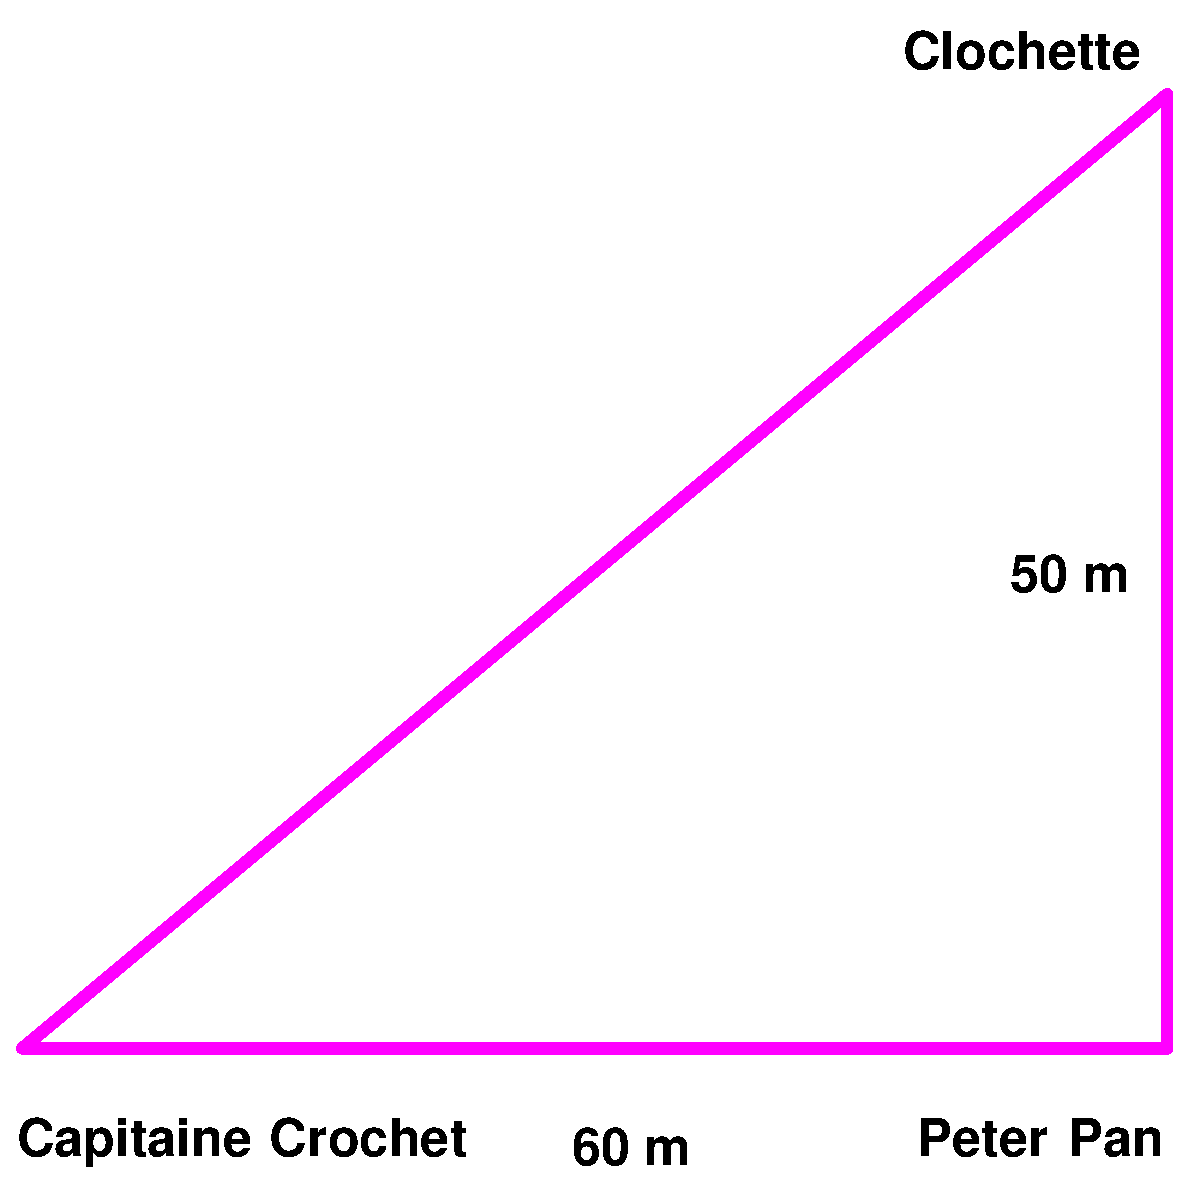
\includegraphics[width=6cm]{triangle24.eps}
% triangle24.eps : 300dpi, width=3.39cm, height=3.39cm, bb=0 0 400 400
    \end{center}

$a^{2}+b^{2}=c^{2}\\
60^{2}+50^{2}=c^{2}\\
3600+2500=c^{2}\\
6100=c^{2}\\
\sqrt{6100}=c\\
c=78,10$ m\\
Cette distance est sup\'erieure \`a 75 m.  La f\'ee Clochette ne peut donc
pas entendre ce que le capitaine Crochet dit.  La r\'eponse est b).\\

485--  La ferme de toit de la maison de Mafalda a la forme d'un triangle
\'equilat\'eral dont les c\^ot\'es mesurent 5 m.  Le p\`ere de Mafalda veut
mettre une poutre pour consolider la ferme de toit.  Il la met \`a l'endroit
qui correspond \`a une hauteur du triangle \'equilat\'eral.  Quelle longueur
de poutre doit-il acheter, sachant qu'il d\'esire consolider deux fermes de
toit de cette forme?\\
a) 4,33 m\\
b) 8,66 m\\
c) 12,99 m\\
d) 17,32 m\\

R\'eponse : b)\\

R\'etroaction :\\
On abaisse une hauteur dans le triangle \'equilat\'eral.  Cette hauteur
forme deux triangles rectangles de 2,5 m de base et de 5 m d'hypot\'enuse.
La hauteur de chacun des triangles rectangles correspond \`a la hauteur du
triangle \'equilat\'eral.  Pour trouver cette hauteur, il faut utiliser le
th\'eor\`eme de Pythagore.\\

$a^{2}+b^{2}=c^{2}\\
2,5^{2}+b^{2}=5^{2}\\
6,25+b^{2}=25\\
b^{2}=18,75\\
b=\sqrt{18,75}\\
b=4,33$\\
Il faut 4,33 m de poutre pour une ferme de toit.  Pour deux fermes de toit,
il faut donc 8,66 m de poutre.  La r\'eponse est b).\\


486-- Un triangle isoc\`ele ABC a deux c\^ot\'es mesurant 20\,cm et un
c\^ot\'e mesurant 12\,cm.  Le sommet A est celui compris entre les deux
c\^ot\'es congrus.  Quelle est la hauteur relative au sommet A?\\
a) $2\sqrt{91}$ cm\\
b) $2\sqrt{109}$ cm\\
c) $4\sqrt{91}$ cm\\
d) $3\sqrt{109}$ cm\\

R\'eponse : a)\\

R\'etroaction : \\
La hauteur relative au sommet A cr\'ee deux triangles rectangles congrus
dont la base est de 6\,cm et l'hypot\'enuse de 20\,cm.  De plus, cette
hauteur est celle de chacun des triangles rectangles.  Il faut utiliser le
th\'eor\`eme de Pythagore.\\
$a^{2}+b^{2}=c^{2}\\
6^{2}+b^{2}=20^{2}\\
36+b^{2}=400\\
b^{2}=364\\
b=\sqrt{364}=2\sqrt{91}$\\
La r\'eponse est donc a).\\

487-- Deux droites parall\`eles sont trac\'ees sur une surface.  En combien
de r\'egions la surface est-elle divis\'ee?\\

R\'eponse : 3\\

R\'etroaction : \\
La surface est divis\'ee en trois r\'egions.\\
\begin{center}
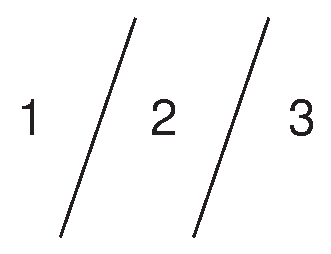
\includegraphics[width=4cm]{487.eps}
\end{center}

488-- Deux droites s\'ecantes sont trac\'ees sur une surface.  En combien de
r\'egions la surface est-elle divis\'ee?\\

R\'eponse : 4\\

R\'etroaction : \\
La surface est divis\'ee en quatre r\'egions.\\
\begin{center}
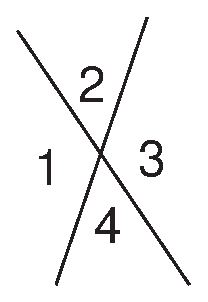
\includegraphics[height=6cm]{488.eps}
\end{center}

489-- Deux droites perpendiculaires sont trac\'ees sur une surface.  En
combien de r\'egions la surface est-elle divis\'ee?\\

R\'eponse : 4\\

R\'etroaction :\\
La surface est divis\'ee en quatre r\'egions.\\
\begin{center}
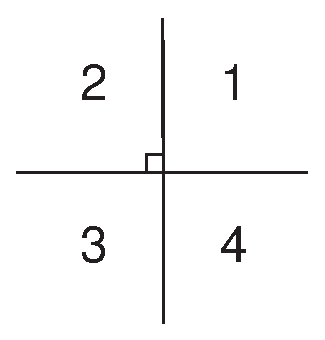
\includegraphics[width=6cm]{489.eps}
\end{center}


490-- En combien de r\'egions un plan divise-t-il l'espace?\\

R\'eponse : 2\\

R\'etroaction : \\
L'espace est divis\'e en deux r\'egions.\\
    \begin{center}
    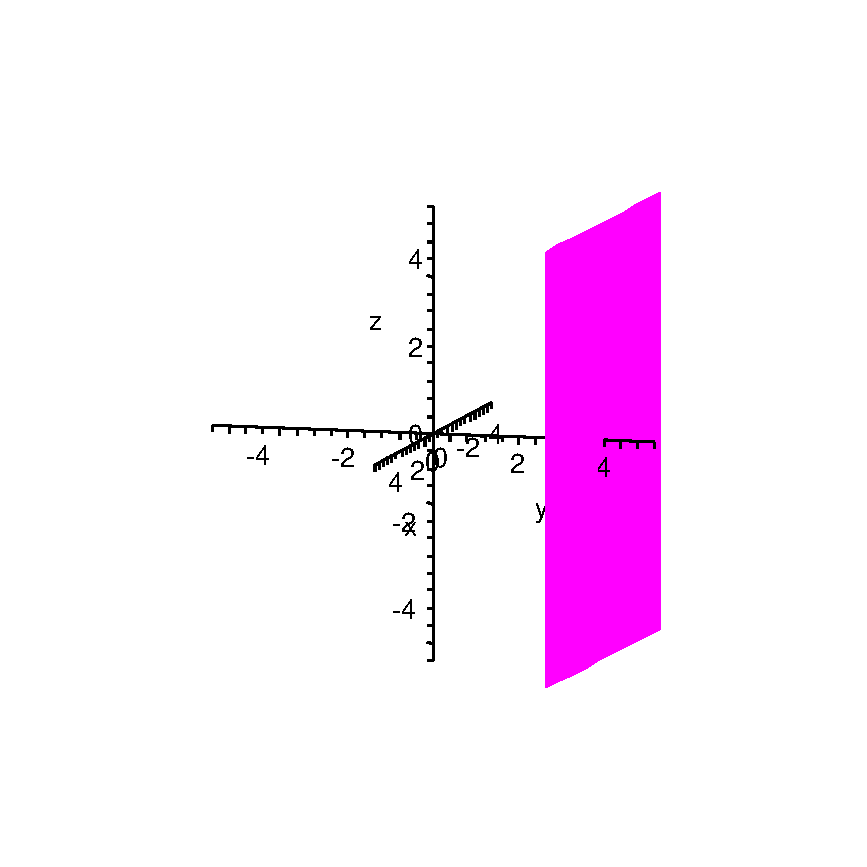
\includegraphics[width=6cm,bb=0 0 400 400]{unplan.eps}
% unplan.eps : 300dpi, width=3.39cm, height=3.39cm, bb=0 0 400 400
    \end{center}

La r\'eponse est 2.\\


492-- En combien de r\'egions deux plans s\'ecants divisent-ils l'espace?\\

R\'eponse : 4\\

R\'etroaction :\\
Les deux plans s\'ecants forment quatre r\'egions dans l'espace.\\
    \begin{center}
    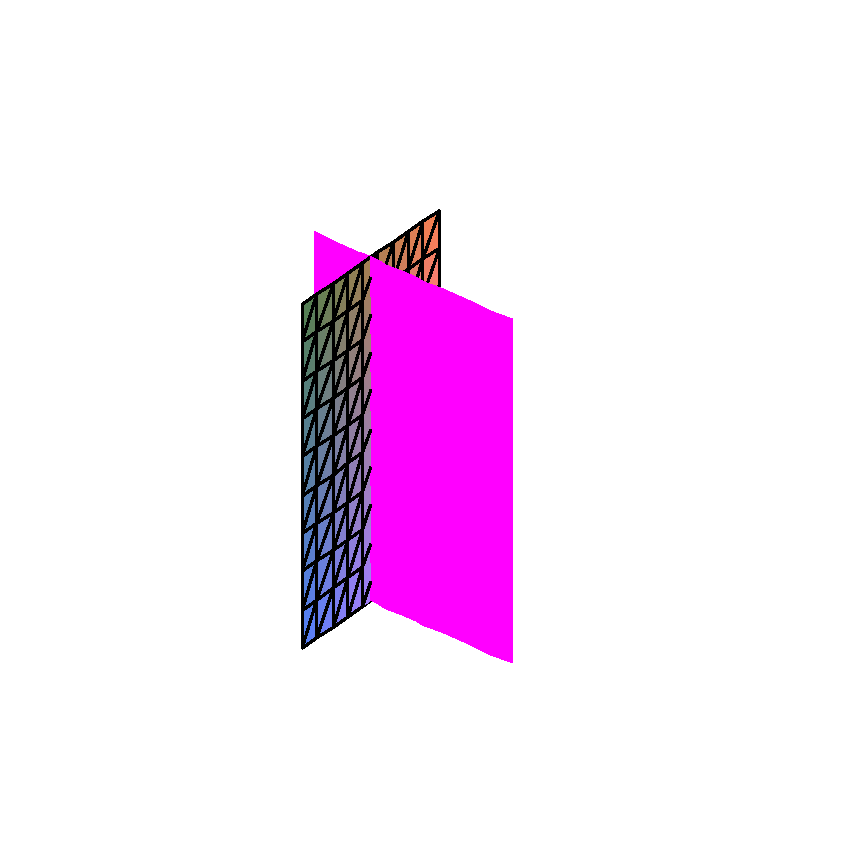
\includegraphics[width=6cm,bb=0 0 400 400]{deuplansecant.eps}
% deuplansecant.eps : 300dpi, width=3.39cm, height=3.39cm, bb=0 0 400 400
    \end{center}
La r\'eponse est 4.\\

493--  Lequel des quatre mots ci-dessous compl\`ete correctement
l'\'enonc\'e suivant : \og Un d\'ecim\`etre cube est \'equivalent
\`a un \ldots\fg ?\\
a) Centilitre\\
b) D\'ecilitre\\
c) Hectolitre\\
d) Litre\\

R\'eponse : d)\\

R\'etroaction : \\
Un d\'ecim\`etre cube est \'equivalent \`a un litre.  La r\'eponse est d).\\

494-- Parmi les quatre mots ci-dessous, lequel compl\`ete
correctement l'\'enonce suivant : \og\`A une pression
atmosph\'erique normale, un litre d'eau p\`ese \`a peu pr\`es $\ldots$\fg ?\\
a) un kilogramme.\\
b) une livre.\\
c) cinq kilogrammes.\\
d) cinq livres.\\

R\'eponse : a)\\

R\'etroaction :
\`A une pression atmosph\'erique normale, un litre d'eau p\`ese \`a peu
pr\`es un kilogramme.  La r\'eponse est donc a).\\

495-- Zorro veut ranger des blocs dans une bo\^ite.  Les blocs mesurent 2 dm
de largeur, 4 dm de longueur et 1 dm de hauteur.  La bo\^ite mesure 6 dm de
largeur, 8 dm de longueur et 3 dm de hauteur.  Quelle quantit\'e maximale de
blocs Zorro peut-il placer dans la bo\^ite?\\
a) 6\\
b) 8\\
c) 9\\
d) 18\\

R\'eponse : d)\\

R\'etroaction : \\
La largeur de la bo\^ite permet de placer trois blocs et la longueur
deux. Il est ainsi possible de disposer six blocs sur un m\^eme
niveau, la hauteur de la bo\^ite permettant la cr\'eation de trois
de ces niveaux. Par cons\'equent, le nombre maximal de blocs que
peut contenir la bo\^ite est
18.  La r\'eponse est d).\\

496-- Sur une \'etag\`ere d'entrep\^ot, Shrek a plac\'e 52 bo\^ites ayant
chacune un volume de 122,7\,cm$^{3}$.  Parmi les quatre choix suivants,
lequel repr\'esente l'espace occup\'e par les 52 bo\^ites? \\
a) 63,804\,m$^{3}$\\
b) 63,804\,cm$^{3}$\\
c) 6380,4\,cm$^{3}$\\
d) $63\,804$\,cm$^{3}$\\

R\'eponse : c)\\

R\'etroaction : \\
Il suffit de multiplier le volume d'une bo\^ite par le nombre de bo\^ites.
\\
122,7\,cm$^{3}\,\times$ 52 = 6380,4\,cm$^{3}$\\
La r\'eponse est donc c).\\

497--  Un camion peut contenir 16 palettes.  Une palette contient 36
bo\^ites occupant chacune un volume de 0,6\,m$^{3}$.  Quel volume ce camion
peut-il transporter?\\
a) 34,56\,m$^{3}$\\
b) 345,6\,m$^{3}$\\
c) 690,6\,m$^{3}$\\
d) 960,6\,m$^{3}$\\

R\'eponse : b)\\

R\'etroaction :\\
Une palette occupe un volume de $36\,\times\,0,6$\,m$^{3}=21,6$\,m$^{3}$.
Par cons\'equent, le camion peut contenir un volume de
$16\,\times\,21,6$\,m$^{3}=345,6$\,m$^{3}$.  La r\'eponse est b).\\

498-- Lequel des quatre \'enonc\'es suivants concernant le volume d'un
prisme est-il vrai?\\
a) Volume = aire de la base $\times$ diagonale\\
b) Volume = aire de la base $\times$ hauteur\\
c) Volume = aire de la base $\times$ largeur\\
d) Volume = aire de la base $\times$ longueur\\

R\'eponse : b)\\

R\'etroaction : \\
Le volume d'un prisme est \'egal \`a l'aire de sa base multipli\'ee par sa
hauteur.\\
La r\'eponse est b).\\

499-- Parmi les quatre choix ci-dessous, lequel compl\`ete
correctement l'\'enonc\'e suivant : \og Deux solides ayant la m\^eme
hauteur ont le m\^eme volume si toutes les sections d\'etermin\'ees
par des plans parall\`eles $\ldots$\fg ?\\
a) ont la m\^eme aire.\\
b) ont le m\^eme volume.\\
c) ont le m\^eme p\'erim\`etre.\\
d) sont de la m\^eme couleur.\\

R\'eponse : a)\\

R\'etroaction : \\
Deux solides ayant la m\^eme hauteur ont le m\^eme volume si toutes les
sections d\'etermin\'ees par des plans parall\`eles ont la m\^eme aire.  La
r\'eponse est a).\\

500-- Shrek a re\c cu une affiche par la poste.  Cette affiche \'etait dans
un cylindre de 5\,cm de diam\`etre et de 10\,cm de hauteur.  Quel \'etait le
volume occup\'e par le cylindre dans le camion de transport?\\
a) $6,25\pi$\,cm$^{3}$\\
b) $31,25\pi$\,cm$^{3}$\\
c) $62,5\pi$\,cm$^{3}$\\
d) $125\pi$\,cm$^{3}$\\

R\'eponse : c)\\

R\'etroaction : \\
Pour calculer le volume d'un cylindre, il suffit de calculer l'aire du
disque formant la base et de la multiplier par la hauteur.  \\
Soit A l'aire du disque et r son rayon.
\begin{eqnarray*}
A &=& \pi r^{2} \\
&=& \pi \times \left( 2,5\right)^{2}\,cm^{2}\\
&=& 6,25\pi\,cm^{2}\\
\end{eqnarray*}
Volume du cylindre = $6,25\pi$\,cm$^{2} \times 10$\,cm
$\,=\,62,5\pi$\,cm$^{3}$\\
La r\'eponse est donc c).\\


502-- Lequel des quatre \'enonc\'es suivants est vrai?\\
a) Si deux prismes ont la m\^eme hauteur, alors ils ont tous les deux le
m\^eme volume.\\
b) Si deux prismes ont la m\^eme hauteur, alors celui qui a le plus grand
volume est celui dont la base a l'aire la plus grande.\\
c) Si deux prismes ont la m\^eme hauteur, alors celui qui a le plus grand
volume est celui dont la base a l'aire la plus petite.\\
d) Si deux prismes ont la m\^eme hauteur, alors celui qui a le plus petit
volume est celui dont la base a l'aire la plus grande.\\

R\'eponse : b)\\

R\'etroaction :
Si deux prismes ont la m\^eme hauteur, alors celui qui a le plus grand
volume est celui dont la base a l'aire la plus grande. La r\'eponse est
b).\\

503-- Lequel des quatre \'enonc\'es suivants est vrai? \\
a) Si deux cylindres ont la m\^eme base, celui qui a le plus petit volume
est celui qui a la plus grande hauteur.\\
b) Si deux cylindres ont la m\^eme base, celui qui a le plus petit volume
est celui qui a la plus petite hauteur.\\
c) Si deux cylindres ont la m\^eme base, le plus grand des deux est celui
qui a la plus petite hauteur.\\
d) Si deux cylindres ont la m\^eme base, ils ont le m\^eme volume.\\

R\'eponse : b)\\

R\'etroaction :  \\
Si deux cylindres ont la m\^eme base, celui qui a le plus petit volume est
celui qui a la plus petite hauteur.  La r\'eponse est donc b).\\

504-- Lequel des choix ci-dessous compl\`ete correctement
l'\'enonc\'e suivant : \og Le volume d'une pyramide triangulaire est
\'egal  $\ldots$ du volume du prisme triangulaire qui lui correspond.\fg?\\
a) \`a la demie\\
b) au tiers\\
c) au quart\\
d) au cinqui\`eme\\

R\'eponse : b)\\

R\'etroaction :  \\
Le volume d'une pyramide triangulaire est \'egal au tiers du volume du
prisme triangulaire qui lui correspond.  La r\'eponse est b).\\

505-- La Belle veut d\'ecorer son arbre de No\"el et elle d\'ecide
de fabriquer ses propres boules de No\"el.  Elle utilise des
sph\`eres de 4\,cm
de rayon.  Pour chaque boule, quelle est l'aire de la surface \`a peindre?\\
a) $8\pi$ cm$^{2}$\\
b) $16\pi$ cm$^{2}$\\
c) $32\pi$ cm$^{2}$\\
d) $64\pi$ cm$^{2}$\\

R\'eponse : d)\\

R\'etroaction : \\
La formule pour trouver l'aire d'une sph\`ere est $4\pi r^{2}$, o\`u $r$ est
le rayon.  \\
Aire d'une sph\`ere = $4\pi\,\times\,4^{2}=4\pi\,\times\,16\,=\,64\pi$\\
Par cons\'equent, la r\'eponse est d).\\

506-- Laquelle des quatre \'egalit\'es suivantes est vraie?\\
a) Volume d'une pyramide = $\frac{1}{4}$(aire de la
base)$\cdot$(hauteur)\\[2mm]
b) Volume d'une pyramide = $\frac{1}{3}$(aire de la
base)$\cdot$(hauteur)\\[2mm]
c) Volume d'une pyramide = $\frac{1}{2}$(aire de la
base)$\cdot$(hauteur)\\[2mm]
d) Volume d'une pyramide = (aire de la base)$\cdot$(hauteur)\\

R\'eponse : b)\\

R\'etroaction :  \\
Volume d'une pyramide = $\frac{1}{3}$(aire de la base)$\cdot$(hauteur)\\
La r\'eponse est donc b).\\

507-- Laquelle des quatre \'egalit\'es suivantes est vraie?\\
a) Volume d'un c\^one = $\frac{1}{4}$(aire de la
base)$\cdot$(hauteur)\\[2mm]
b) Volume d'un c\^one = $\frac{1}{3}$(aire de la
base)$\cdot$(hauteur)\\[2mm]
c) Volume d'un c\^one = $\frac{1}{2}$(aire de la
base)$\cdot$(hauteur)\\[2mm]
d) Volume d'un c\^one = (aire de la base)$\cdot$(hauteur)\\

R\'eponse : b)\\

R\'etroaction :  \\
Volume d'un c\^one = $\frac{1}{3}$(aire de la base)$\cdot$(hauteur)\\
La r\'eponse est donc b).\\

508-- Laquelle des quatre \'egalit\'es suivantes est vraie?\\
a) Volume d'un prisme = $\frac{1}{4}$(aire de la
base)$\cdot$(hauteur)\\[2mm]
b) Volume d'un prisme = $\frac{1}{3}$(aire de la
base)$\cdot$(hauteur)\\[2mm]
c) Volume d'un prisme = $\frac{1}{2}$(aire de la
base)$\cdot$(hauteur)\\[2mm]
d) Volume d'un prisme = (aire de la base)$\cdot$(hauteur)\\

R\'eponse : d)\\

R\'etroaction :
Volume d'un prisme = (aire de la base)$\cdot$(hauteur)\\
Par cons\'equent, la r\'eponse est d).\\

509-- Parmi les quatre d\'efinitions suivantes, laquelle est celle de
l'apoth\`eme d'un polygone r\'egulier?\\
a) C'est le segment reliant deux coins oppos\'es du polygone r\'egulier.\\
b) C'est le segment reliant les deux coins les plus \'eloign\'es du polygone
r\'egulier.\\
c) C'est le segment reliant le centre du polygone r\'egulier et un de ses
coins.\\
d) C'est le segment reliant perpendiculairement le centre du polygone
r\'egulier et un de ses c\^ot\'es.\\

R\'eponse : d)\\

R\'etroaction :  \\
C'est le segment reliant perpendiculairement le centre du polygone
r\'egulier et un de ses c\^ot\'es.  La r\'eponse est d).\\

510-- Parmi les quatre d\'efinitions suivantes, laquelle est celle de
l'apoth\`eme d'une pyramide r\'eguli\`ere droite?\\
a) C'est le segment correspondant \`a la hauteur des triangles formant les
faces lat\'erales d'une pyramide r\'eguli\`ere droite.  \\
b) C'est le segment correspondant \`a la hauteur des triangles form\'es en
reliant les coins oppos\'es de la base d'une pyramide r\'eguli\`ere
droite.\\
c) C'est le segment correspondant \`a la mesure des c\^ot\'es des triangles
isoc\`eles formant les faces lat\'erales d'une pyramide r\'eguli\`ere
droite.\\
d) C'est le segment correspondant \`a la mesure d'un des c\^ot\'es de la
base d'une pyramide r\'eguli\`ere droite.\\

R\'eponse : a)\\

R\'etroaction :
C'est le segment correspondant \`a la hauteur des triangles formant les
faces lat\'erales d'une pyramide r\'eguli\`ere droite.  La r\'eponse est
donc a).\\


512--  Parmi les quatre isom\'etries ci-dessous, laquelle conserve
l'orientation de la figure finale par rapport \`a la figure initiale et ne
cr\'ee pas de traces parall\`eles entre ces deux figures?\\
a) R\'eflexion\\
b) Rotation\\
c) Sym\'etrie gliss\'ee\\
d) Translation\\

R\'eponse : b)\\

R\'etroaction :\\
La rotation conserve l'orientation de la figure finale par rapport \`a la
figure initiale et ne cr\'ee pas de traces parall\`eles entre ces deux
figures. La r\'eponse est b).\\

513--  Parmi les quatre isom\'etries ci-dessous, laquelle ne conserve pas
l'orientation de la figure finale par rapport \`a la figure initiale et
cr\'ee des traces parall\`eles entre ces deux figures?\\
a) R\'eflexion\\
b) Rotation\\
c) R\'eflexion gliss\'ee\\
d) Translation\\

R\'eponse : a)\\

R\'etroaction :\\
La r\'eflexion ne conserve pas l'orientation de la figure finale par rapport
\`a la figure initiale, en fait, elle l'inverse. De plus, elle cr\'ee des
traces parall\`eles entre la figure initiale et la figure finale.  La
r\'eponse est a).\\

514--  Parmi les quatre isom\'etries ci-dessous, laquelle ne conserve pas
l'orientation de la figure finale par rapport \`a la figure initiale et ne
cr\'ee pas de traces parall\`eles entre ces deux figures?\\
a) R\'eflexion\\
b) R\'eflexion gliss\'ee\\
c) Rotation\\
d) Translation\\

R\'eponse : b)\\

R\'etroaction :\\
La r\'eflexion gliss\'ee ne conserve pas l'orientation de la figure finale
par rapport \`a la figure initiale, en fait, elle l'inverse. De plus, elle
ne cr\'ee pas de traces parall\`eles entre ces deux figures.  La r\'eponse
est b).\\

515-- La piscine creus\'ee de Pocahontas a la forme d'un prisme
rectangulaire.  Elle mesure 9\,m de long, 5\,m de large et 2\,m de
profondeur.  Combien de litres d'eau contient-elle lorsqu'elle est remplie
aux $\frac{9}{10}$?\\
a) 81 L\\
b) 90 L\\
c) $81\,000$ L\\
d) $90\,000$ L\\

R\'eponse : c)\\

R\'etroaction :\\
Lorsque la piscine est pleine, elle contient $9$\,m
$\times\,5$\,m $\times\,2$\,m $=\,90$\,m$^{3}$ d'eau.\\[2mm]
$\frac{9}{10}$ de 90\,m$^{3}$ =
$\frac{9}{10}\times90$\,m$^{3}=81$\,m$^{3}$\\[2mm]
81\,m$^{3}=81\,000$ dm$^{3}=81\,000$ L\\[2mm]
La r\'eponse est donc c).\\

516-- Geppetto poss\`ede une collection de 105 petits cubes dont les
ar\^etes mesurent 1\,cm.  S'il les utilise pour former le plus grand cube
possible, combien de petits cubes utilise-t-il?  \\

R\'eponse : 64\\

R\'etroaction :  \\
$4\times4\times4=64$\\
$5\times5\times5=125$\\
Geppetto forme donc un cube de 4 par 4 par 4 et utilise 64 petits cubes.  \\

517-- Parmi les quatre choix ci-dessous, lequel compl\`ete
correctement l'\'enonc\'e suivant : \og Toute translation et toute
homoth\'etie transforment une droite en $\ldots$\fg ?\\
a) une droite oblique.\\
b) une droite ondul\'ee.\\
c) une droite parall\`ele.\\
d) une droite perpendiculaire.\\

R\'eponse : c)\\

R\'etroaction : \\
Toute translation et toute homoth\'etie transforment une droite en une
droite parall\`ele.  La r\'eponse est c).\\


518-- Dans un tableau de d\'epouillement de donn\'ees, \`a quoi correspond
l'effectif?\\
a) Au nom des diff\'erentes donn\'ees\\
b) Au nombre de cat\'egories diff\'erentes\\
c) Au nombre de colonnes dans le tableau de d\'epouillement\\
d) Au nombre de fois qu'une valeur est apparue\\

R\'eponse : d)\\

R\'etroaction : \\
L'effectif est le nombre de fois qu'une valeur est apparue.  La r\'eponse
est d).\\

519-- Parmi les quatre expressions ci-dessous, laquelle permet de calculer
une moyenne arithm\'etique?\\
a) $\frac{x_1\,+\,x_2\,+\,x_3\,+\,\ldots\,+\,x_n}{n}$\\[2mm]
b)
$\sqrt{\frac{x_1^{2}\,+\,x_2^{2}\,+\,x_3^{2}\,+\,\ldots\,+\,x_n^{2}}{n}}$\\[2mm]
c) $\sqrt[n]{x_1 \cdot x_2 \cdot x_3 \cdot \ldots \cdot x_n}$\\[2mm]
d)
$\frac{n}{\frac{1}{x_1}\,+\,\frac{1}{x_2}\,+\,\frac{1}{x_3}\,+\,\cdots\,+\,\frac{1}{x_n}}$\\

R\'eponse : a)\\

R\'etroaction : \\
Moyenne arithm\'etique =
$\frac{x_1\,+\,x_2\,+\,x_3\,+\,\ldots\,+\,x_n}{n}$\\[2mm]
Moyenne quadratique =
$\sqrt{\frac{x_1^{2}\,+\,x_2^{2}\,+\,x_3^{2}\,+\,\ldots\,+\,x_n^{2}}{n}}$\\[2mm]
Moyenne g\'eom\'etrique = $\sqrt[n]{x_1\cdot x_2\cdot x_3 \cdot \ldots \cdot
x_n}$\\[2mm]
Moyenne harmonique =
$\frac{n}{\frac{1}{x_1}\,+\,\frac{1}{x_2}\,+\,\frac{1}{x_3}\,+\,\cdots\,+\,\frac{1}{x_n}}$\\[2mm]
La r\'eponse est donc a).\\

520-- Parmi les quatre expressions ci-dessous, laquelle permet de calculer
une moyenne quadratique?\\
a) $\frac{x_1\,+\,x_2\,+\,x_3\,+\,\ldots\,+\,x_n}{n}$\\[2mm]
b)
$\sqrt{\frac{x_1^{2}\,+\,x_2^{2}\,+\,x_3^{2}\,+\,\ldots\,+\,x_n^{2}}{n}}$\\[2mm]
c) $\sqrt[n]{x_1 \cdot x_2 \cdot x_3 \cdot \ldots \cdot x_n}$\\[2mm]
d)
$\frac{n}{\frac{1}{x_1}\,+\,\frac{1}{x_2}\,+\,\frac{1}{x_3}\,+\,\cdots\,+\,\frac{1}{x_n}}$\\

R\'eponse : b)\\

R\'etroaction : \\
Moyenne arithm\'etique =
$\frac{x_1\,+\,x_2\,+\,x_3\,+\,\ldots\,+\,x_n}{n}$\\[2mm]
Moyenne quadratique =
$\sqrt{\frac{x_1^{2}\,+\,x_2^{2}\,+\,x_3^{2}\,+\,\ldots\,+\,x_n^{2}}{n}}$\\[2mm]
Moyenne g\'eom\'etrique = $\sqrt[n]{x_1\cdot x_2\cdot x_3 \cdot \ldots \cdot
x_n}$\\[2mm]
Moyenne harmonique =
$\frac{n}{\frac{1}{x_1}\,+\,\frac{1}{x_2}\,+\,\frac{1}{x_3}\,+\,\cdots\,+\,\frac{1}{x_n}}$\\[2mm]
La r\'eponse est donc b).\\


522-- Parmi les quatre expressions ci-dessous, laquelle permet de calculer
une moyenne harmonique?\\
a) $\frac{x_1\,+\,x_2\,+\,x_3\,+\,\ldots\,+\,x_n}{n}$\\[2mm]
b)
$\sqrt{\frac{x_1^{2}\,+\,x_2^{2}\,+\,x_3^{2}\,+\,\ldots\,+\,x_n^{2}}{n}}$\\[2mm]
c) $\sqrt[n]{x_1 \cdot x_2 \cdot x_3 \cdot \ldots \cdot x_n}$\\[2mm]
d)
$\frac{n}{\frac{1}{x_1}\,+\,\frac{1}{x_2}\,+\,\frac{1}{x_3}\,+\,\cdots\,+\,\frac{1}{x_n}}$\\

R\'eponse : d)\\

R\'etroaction : \\
Moyenne arithm\'etique =
$\frac{x_1\,+\,x_2\,+\,x_3\,+\,\ldots\,+\,x_n}{n}$\\[2mm]
Moyenne quadratique =
$\sqrt{\frac{x_1^{2}\,+\,x_2^{2}\,+\,x_3^{2}\,+\,\ldots\,+\,x_n^{2}}{n}}$\\[2mm]
Moyenne g\'eom\'etrique = $\sqrt[n]{x_1\cdot x_2\cdot x_3 \cdot \ldots \cdot
x_n}$\\[2mm]
Moyenne harmonique =
$\frac{n}{\frac{1}{x_1}\,+\,\frac{1}{x_2}\,+\,\frac{1}{x_3}\,+\,\cdots\,+\,\frac{1}{x_n}}$\\[2mm]
Par cons\'equent, la r\'eponse est d).\\

523-- Qu'est-ce que le mode d'une distribution o\`u les donn\'ees ne sont
pas regroup\'ees en classes?\\
a) C'est la plus grande valeur.\\
b) C'est la plus petite valeur.\\
c) C'est la valeur la plus fr\'equente.\\
d) C'est la valeur la moins fr\'equente.\\

R\'eponse : c)\\

R\'etroaction : \\
Dans une distribution o\`u les donn\'ees ne sont pas regroup\'ees en
classes, le mode est la valeur la plus fr\'equente.  La r\'eponse est c).\\

524-- Qu'est-ce que le mode d'une distribution o\`u les donn\'ees sont
regroup\'ees en classes?\\
a) C'est la classe avec le plus grand effectif.\\
b) C'est la classe avec le plus petit effectif.\\
c) C'est la derni\`ere classe.\\
d) C'est la premi\`ere classe.\\

R\'eponse : a)\\

R\'etroaction : \\
Le mode d'une distribution o\`u les donn\'ees sont regroup\'ees en classes
est la classe avec le plus grand effectif.  En fait, on l'appelle la classe
modale.  La r\'eponse est a).\\

525-- Dans une distribution o\`u les donn\'ees ne sont pas regroup\'ees en
classes, qu'est-ce que l'\'etendue?\\
a) C'est la diff\'erence entre la plus grande et la plus petite donn\'ee.\\
b) C'est le produit de la plus grande et de la plus petite donn\'ee.\\
c) C'est le quotient de la plus grande donn\'ee par la plus petite
donn\'ee.\\
d) C'est la somme de la plus grande et de la plus petite donn\'ee.\\

R\'eponse : a)\\

R\'etroaction : \\
L'\'etendue est la diff\'erence entre la plus grande et la plus petite
donn\'ee.  La r\'eponse est a).\\

526-- Dans une distribution o\`u les donn\'ees sont regroup\'ees en classes,
qu'est-ce que l'\'etendue?\\
a) C'est la diff\'erence entre la limite sup\'erieure de la derni\`ere
classe et la limite inf\'erieure de la premi\`ere classe.\\
b) C'est le produit de la limite sup\'erieure de la derni\`ere classe et de
la limite inf\'erieure de la premi\`ere classe.\\
c) C'est le quotient de la limite sup\'erieure de la derni\`ere classe par
la limite inf\'erieure de la premi\`ere classe.\\
d) C'est la somme de la limite sup\'erieure de la derni\`ere classe et de la
limite inf\'erieure de la premi\`ere classe.\\

R\'eponse : a) \\

R\'etroaction : \\
Dans une distribution o\`u les donn\'ees sont regroup\'ees en classes,
l'\'etendue est la diff\'erence entre la limite sup\'erieure de la classe la
plus \'elev\'ee et la limite inf\'erieure de la classe la moins \'elev\'ee.
La r\'eponse est a).\\

527-- Dans une distribution, par quel symbole repr\'esente-t-on
g\'en\'eralement la moyenne?\\
a) $\overline{w}$\\
b) $\overline{x}$\\
c) $\overline{y}$\\
d) $\overline{z}$\\

R\'eponse : b)\\

R\'etroaction : \\
La moyenne est repr\'esent\'ee par $\overline{x}$.  La r\'eponse est b).\\

528-- Voici la liste des r\'esultats sur 40 obtenus par 12 \'el\`eves lors
d'un examen : 25, 26, 27, 27, 27, 29, 32, 33, 35, 36, 37, 39.  Quelle est
l'\'etendue de cette distribution?\\

R\'eponse : 14\\

R\'etroaction : \\
Pour trouver l'\'etendue, il suffit de faire la diff\'erence entre la plus
grande et la plus petite donn\'ee.  \\
$39-25=14$\\
La r\'eponse est 14.\\

529-- Voici la liste des r\'esultats sur 40 obtenus par 12 \'el\`eves lors
d'un examen : 25, 26, 27, 27, 27, 29, 32, 33, 35, 36, 37, 39.  Quelle est le
mode de cette distribution?\\

R\'eponse : 27\\

R\'etroaction : \\
Le mode est la donn\'ee la plus fr\'equente de la distribution.  La
r\'eponse est 27.\\

530-- Voici la liste des r\'esultats sur 40 obtenus par 12 \'el\`eves lors
d'un examen : 25, 26, 27, 27, 27, 29, 32, 33, 35, 36, 37, 39.  Parmi les
quatre choix ci-dessous, lequel donne la moyenne de cette distribution?\\
a) $27,96\overline{4}$\\
b) $29,08\overline{5}$\\
c) $31,08\overline{3}$\\
d) $35,69\overline{3}$\\

R\'eponse : c) \\

R\'etroaction : \\
Voici le calcul \`a faire pour trouver la moyenne :\\[2mm]
$\frac{25\,+\,26\,+\,27\,+\,27\,+\,27\,+\,29\,+\,32\,+\,33\,+\,35\,+\,36\,+\,37\,+\,39}{12}=31,08\overline{3}$\\[2mm]
La r\'eponse est donc c).\\


532-- Quelle est la m\'ediane de l'ensemble de donn\'ees 13, 16, 10, 13, 17,
15, 14?

R\'eponse : 14\\

R\'etroaction :\\
La m\'ediane est la valeur qui r\'epartit les donn\'ees en deux ensembles
qui ont exactement le m\^eme nombre de donn\'ees, un qui contient les
donn\'ees inf\'erieures \`a la m\'ediane et l'autre qui contient les
donn\'ees qui lui sont sup\'erieures.  Il faut commencer par classer les
donn\'ees en ordre croissant.\\
10, 13, 13, 14, 15, 16, 17 \\
La r\'eponse est 14.\\

533-- Avant son dernier devoir de math\'ematiques de l'\'etape, Zazu avait
une moyenne de 18.  Il n'a vraiment rien compris du dernier devoir et il a
eu z\'ero.  Par contre, sa moyenne ne baisse pas trop : elle est de 16
apr\`es ce devoir.  Combien de devoirs de math\'ematiques Zazu a-t-il eus
\`a cette \'etape?\\

R\'eponse : 9\\

R\'etroaction : \\
Posons $n$ = nombre de devoirs dans l'\'etape.\\
Soit $r_i$ la note obtenue pour le $i^{e}$ devoir.\\[2mm]
On sait que
$\frac{r_{1}\,+\,r_{2}\,+\,r_{3}\,+\,\ldots\,+\,r_{n-1}}{n-1}=18$,\\[2mm]
c'est-\`a-dire $r_{1}\,+\,r_{2}\,+\,\ldots\,+\,r_{n-1} =18(n-1)$. \qquad
(\'equation 1)\\[2mm]
On sait aussi que \\[2mm]
$\frac{r_{1}\,+\,r_{2}\,+\,\ldots\,+\,r_{n-1}\,+\,r_{n}}{n}=16$.\\[2mm]
Or, $r_{n}=0$.  On a donc \\[2mm]
$\frac{r_{1}\,+\,r_{2}\,+\,r_{3}\,+\,\ldots\,+\,r_{n-1}\,+\,0}{n}=\frac{r_{1}\,+\,r_{2}\,+\,r_{3}\,+\,\ldots\,+\,r_{n-1}}{n}=16$,\\[2mm]
c'est-\`a-dire $r_{1}\,+\,r_{2}\,+\,r_{3}\,+\,\ldots\,+\,r_{n-1}=16n$ \qquad
(\'equation 2)\\[2mm]
Comme on a isol\'e
$r_{1}\,+\,r_{2}\,+\,r_{3}\,+\,\ldots\,+\,r_{n-1}$ dans les
\'equations 1 et 2,
on peut \'ecrire $18\left( n-1\right) = 16n$.\\
$18n-18=16n\\
2n=18\\
n=9$\\
Zazu a eu 9 devoirs durant l'\'etape.\\


534-- Parmi les quatre \'egalit\'es suivantes, laquelle est vraie?\\
a) $3^{-1}>2^{-1}$\\
b) $3^{-1}>3^{1}$\\
c) $3^{-1}>3^{0}$\\
d) $3^{-1}>4^{-1}$\\

R\'eponse : d)\\

R\'etroaction : \\
$3^{-1}=\frac{1}{3}\\[2mm]
4^{-1}=\frac{1}{4}\\[2mm]
\frac{1}{3}>\frac{1}{4}$\\[2mm]
Donc $3^{-1}>4^{-1}$.\\[2mm]
La r\'eponse est d).\\

535-- Parmi les quatre nombres ci-dessous, lequel repr\'esente
$256^{\frac{1}{4}}$?\\
a) 4\\
b) 16\\
c) 32\\
d) 64\\

R\'eponse : a)\\

R\'etroaction : \\
L'expression $256^{\frac{1}{4}}$ est \'equivalente \`a la racine quatri\`eme
de 256.  \\
Comme $4^{4} = 256$, on a $4=\sqrt[4]{256}$ \\
La r\'eponse est donc a).\\

536-- Combien de fois peut-on soustraire 47 de 356 avant d'atteindre un
nombre n\'egatif?\\

R\'eponse : 7\\

R\'etroaction : \\
$356-47=309\\
309-47=262\\
262-47=215\\
215-47=168\\
168-47=121\\
121-47=74\\
74-47=27\\
27-47=-20$\\
Il est possible de soustraire sept fois 47 de 356.  La r\'eponse est 7.\\


537-- Parmi les quatre choix ci-dessous, lequel repr\'esente
$b\,+\,b\,+\,b\,+\,b\times b\times b \times b \times b$?\\
a) $3b\,+\,b^{5}$\\
b) $4b\,+\,b^{4}$\\
c) $4b^{4}$\\
d) $4b^{8}$\\


R\'eponse : a)\\

R\'etroaction : \\
$b\,+\,b\,+\,b\,+\,b\times b\times b \times b \times b= 3b\,+\,b^{5}$\\
La r\'eponse est a).\\

538-- Le triple d'un nombre additionn\'e \`a son cinqui\`eme donne 75.
Parmi les quatre \'equations suivantes, laquelle traduit cet \'enonc\'e?\\
a) $3n\,+\,5b=75$\\[2mm]
b) $3n\,+\,5n=75$\\[2mm]
c) $3n\,+\,\frac{n}{5}=75$\\[2mm]
d) $3n\,+\,\frac{b}{5}=75$\\

R\'eponse : c)\\

R\'etroaction : \\
L'\'equation qui traduit la mise en situation est $3n\,+\,\frac{n}{5}=75$.
La r\'eponse est donc c).\\


539-- Parmi les quatre choix suivants, lequel est une \'equation du premier
degr\'e o\`u $x$ est la variable ind\'ependante, $y$ la variable
d\'ependante et $a$ et $b$ des coefficients?\\
a) $y=ax\,+\,b^{2}$ \\
b) $y=ax^{2}\,+\,b$\\
c) $y=\left( ax\right) ^{2}\,+\,b$\\
d) $y=a^{2}x^{2}\,+\,b$\\

R\'eponse : a)\\

R\'etroaction : \\
La r\'eponse est $y=ax\,+\,b^{2}$, donc a). \\

540-- Parmi les quatre choix ci-dessous, lequel compl\`ete le mieux
l'\'enonc\'e suivant : \og Dans une relation de variation inverse,
le taux de variation est $\ldots$\fg ?\\
a) constant.\\
b) tr\`es grand.\\
c) tr\`es petit.\\
d) variable.\\

R\'eponse : d)\\

R\'etroaction : \\
Dans une relation de variation inverse, le taux de variation est variable.
Voici un graphique repr\'esentant une telle situation.\\
    \begin{center}
    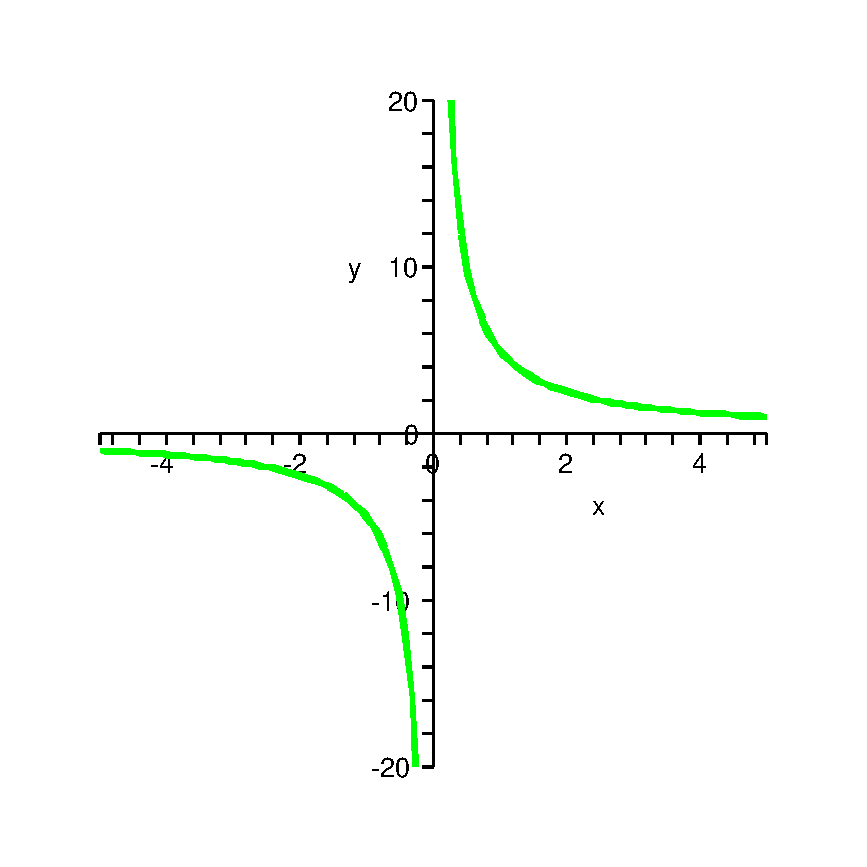
\includegraphics[width=6cm,bb=0 0 400 400]{fonction16.eps}
% fonction16.eps : 300dpi, width=3.39cm, height=3.39cm, bb=0 0 400 400
    \end{center}

La r\'eponse est d).\\


542-- Parmi les quatre choix ci-dessous, lequel se rapporte \`a une relation
de variation inverse?\\[2mm]
a) Constante = $\frac{\textrm{variable d\'ependante}}{\textrm{variable
ind\'ependante}}$\\[2mm]
b) Constante = $\frac{\textrm{variable ind\'ependante}}{\textrm{variable
d\'ependante}}$\\[2mm]
c) Variable d\'ependante = $\frac{\textrm{constante}}{\textrm{variable
ind\'ependante}}$\\[2mm]
d) Variable ind\'ependante = $\frac{\textrm{constante}}{\textrm{variable
ind\'ependante}}$\\

R\'eponse : c)\\

R\'etroaction : \\
L'expression suivante est celle qui se rapporte \`a une relation de
variation inverse:\\[2mm]
variable d\'ependante = $\frac{\textrm{constante}}{\textrm{variable
ind\'ependante}}$.\\[2mm]
Voici un graphique d'une telle relation.
    \begin{center}
    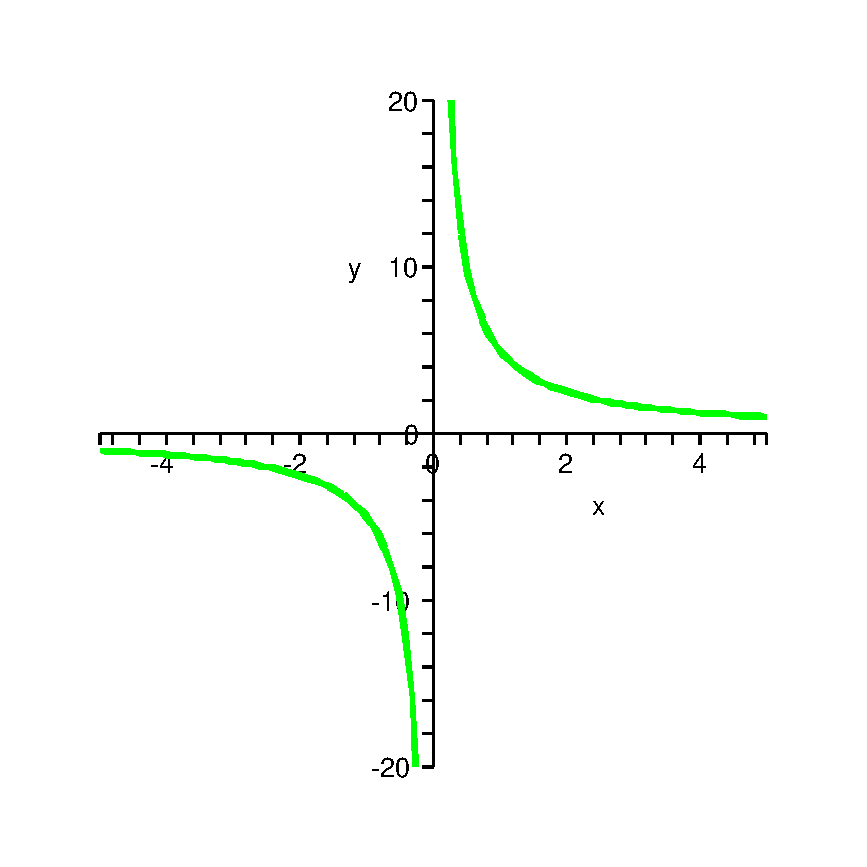
\includegraphics[width=6cm,bb=0 0 400 400]{fonction16.eps}
% fonction16.eps : 300dpi, width=3.39cm, height=3.39cm, bb=0 0 400 400
    \end{center}
La r\'eponse est c).\\

543-- Parmi les quatre choix ci-dessous, lequel est vrai?\\
a) Dans une relation de variation inverse, la courbe ne peut pas couper
l'axe des ordonn\'ees.\\
b) Dans une relation de variation inverse, la courbe peut couper l'axe des
abscisses.\\
c) Dans une relation de variation inverse, la courbe peut couper l'axe des
ordonn\'ees.\\
d) Dans une relation de variation inverse, la courbe peut couper l'axe des
abscisses et l'axe des ordonn\'ees.\\

R\'eponse : a)\\

R\'etroaction : \\
Dans une relation de variation inverse, la courbe ne peut pas couper
l'axe des ordonn\'ees. Voici un graphique d'une telle relation.
    \begin{center}
    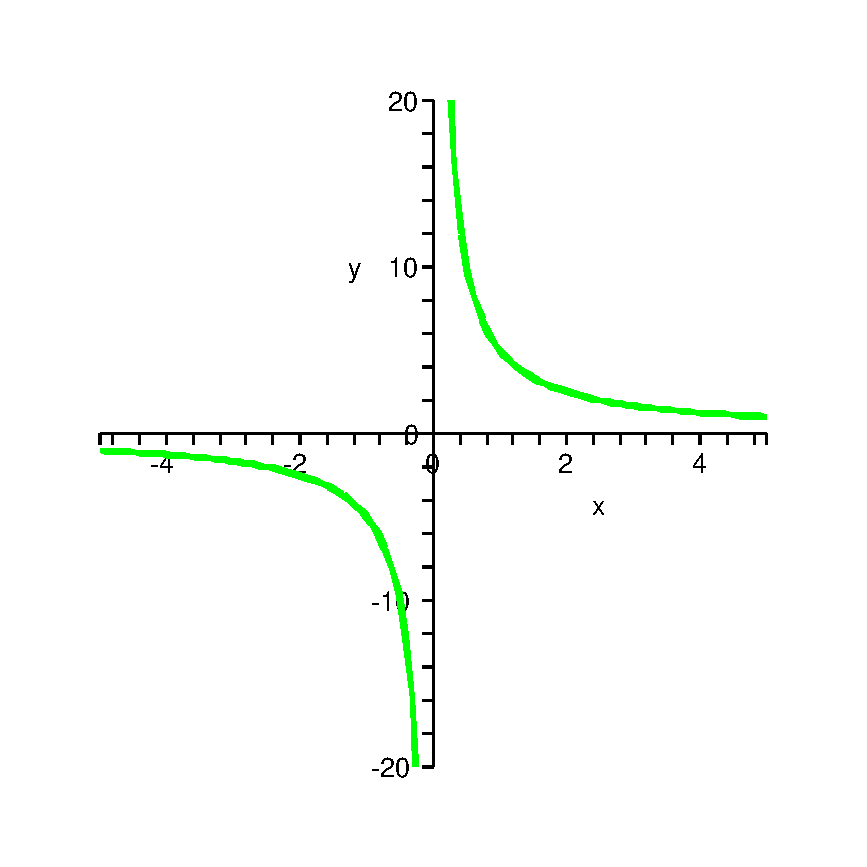
\includegraphics[width=6cm,bb=0 0 400 400]{fonction16.eps}
% fonction16.eps : 300dpi, width=3.39cm, height=3.39cm, bb=0 0 400 400
    \end{center}
La r\'eponse est a).\\

544-- Dans un triangle rectangle, lequel des rapports suivants permet de
trouver la tangente d'un angle?\\[2mm]
a) $\frac{\textrm{mesure du c\^ot\'e adjacent}}{\textrm{mesure de
l'hypot\'enuse}}$\\[2mm]
b) $\frac{\textrm{mesure du c\^ot\'e oppos\'e}}{\textrm{mesure du c\^ot\'e
adjacent}}$\\[2mm]
c) $\frac{\textrm{mesure du c\^ot\'e oppos\'e}}{\textrm{mesure de
l'hypot\'enuse}}$\\[2mm]
d) $\frac{\textrm{mesure de l'hypot\'enuse}}{\textrm{mesure du c\^ot\'e
adjacent}}$\\

R\'eponse : b)\\

R\'etroaction : \\
Cosinus d'un angle = $\frac{\textrm{mesure du c\^ot\'e
adjacent}}{\textrm{mesure de l'hypot\'enuse}}$\\[2mm]
Tangente d'un angle = $\frac{\textrm{mesure du c\^ot\'e
oppos\'e}}{\textrm{mesure du c\^ot\'e adjacent}}$\\[2mm]
Sinus d'un angle = $\frac{\textrm{mesure du c\^ot\'e
oppos\'e}}{\textrm{mesure de l'hypot\'enuse}}$\\[2mm]
S\'ecante d'un angle =  $\frac{\textrm{mesure de
l'hypot\'enuse}}{\textrm{mesure du c\^ot\'e adjacent}}$\\[2mm]
La r\'eponse est donc b).\\

545-- Parmi les choix suivants, lequel s'applique \`a une relation de
variation en escalier?\\
a) Le graphique est form\'e d'un segment continu et horizontal. \\
b) Le graphique est form\'e de segments horizontaux, habituellement ferm\'es
\`a une extr\'emit\'e et ouverts \`a l'autre.\\
c) Le graphique est form\'e de segments horizontaux et verticaux,
habituellement ferm\'es \`a une extr\'emit\'e et ouverts \`a l'autre.\\
d) Le graphique est form\'e d'une multitude de segments horizontaux,
verticaux ou obliques, ferm\'es \`a une extr\'emit\'e et ouverts \`a
l'autre.\\

R\'eponse : b)\\

R\'etroaction : \\
Le graphique est form\'e de segments horizontaux, habituellement ferm\'es
\`a une extr\'emit\'e et ouverts \`a l'autre.
   \begin{center}
    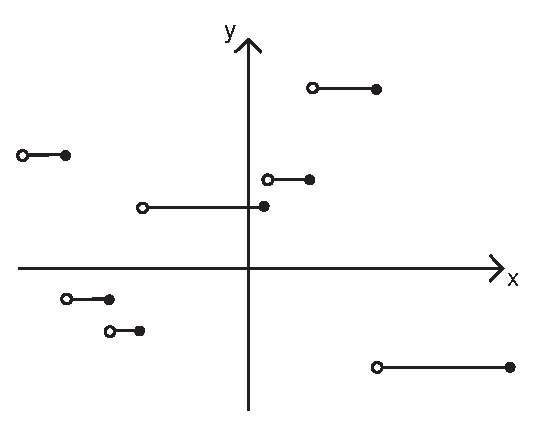
\includegraphics[height=3.39cm]{545.eps}
% napperon.eps : 300dpi, width=3.39cm, height=3.39cm, bb=0 0 400 400
    \end{center}
La r\'eponse est b).\\

546-- Parmi les quatre situations suivantes, laquelle est une situation de
variation en escalier?\\
a) Dans un stationnement, le prix est de 3\,\$ pour une heure ou moins.
Apr\`es une heure, le prix devient 2\,\$ la demi-heure ou fraction de
demi-heure, avec un maximum de 8\,\$ par jour.  \\
b) Un m\'ecanicien a des honoraires de base de 30\,\$ et demande 25\,\$ de
l'heure.\\
c) Un professeur de musique facture 40\,\$ de l'heure.\\
d) Une secr\'etaire a un salaire fixe de 450\,\$ par semaine, peu importe le
nombre d'heures travaill\'ees.\\

R\'eponse : a) \\

R\'etroaction : \\
Dans un stationnement, le prix est de 3\,\$ pour une heure ou moins.
Apr\`es une heure, il devient 2\,\$ la demi-heure ou fraction de demi-heure,
avec un maximum de 8\,\$ par jour.
   \begin{center}
    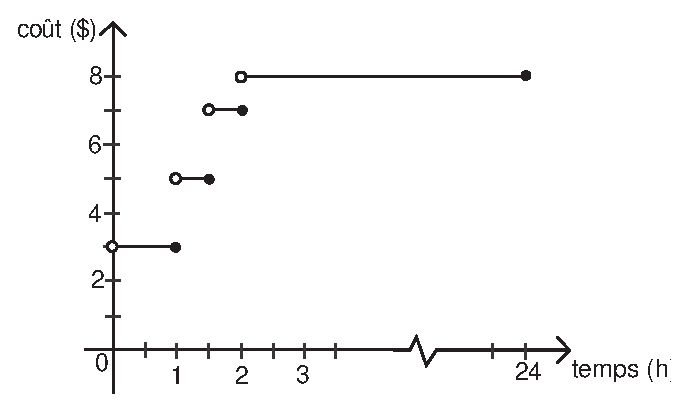
\includegraphics[height=3.39cm]{546.eps}
% napperon.eps : 300dpi, width=3.39cm, height=3.39cm, bb=0 0 400 400
    \end{center}
La r\'eponse est a).\\

547-- Parmi les quatre choix ci-dessous, lequel repr\'esente une relation de
variation exponentielle?\\[2mm]
a) $\textrm{Constante}=\textrm{variable
d\'ependante}\times\left(\textrm{base}\right) ^{\textrm{variable
ind\'ependante}}$\\[2mm]
b) $\textrm{Variable
d\'ependante}=\textrm{constante}\times\left(\textrm{base}\right)
^{\textrm{variable ind\'ependante}}$\\[2mm]
c) $\textrm{Variable
d\'ependante}=\textrm{variable
ind\'ependante}\times\left(\textrm{base}\right)
^{\textrm{constante}}$\\ [2mm]
d) $\textrm{Variable
ind\'ependante}=\textrm{constante}\times\left(\textrm{base}\right)
^{\textrm{variable d\'ependante}}$\\

R\'eponse : b)\\

R\'etroaction : \\
La relation de variation exponentielle est repr\'esent\'ee par l'expression
suivante:\\[2mm]
$\textrm{variable
d\'ependante}=\textrm{constante}\times\left(\textrm{base}\right)
^{\textrm{variable ind\'ependante}}.$\\[2mm]
   \begin{center}
    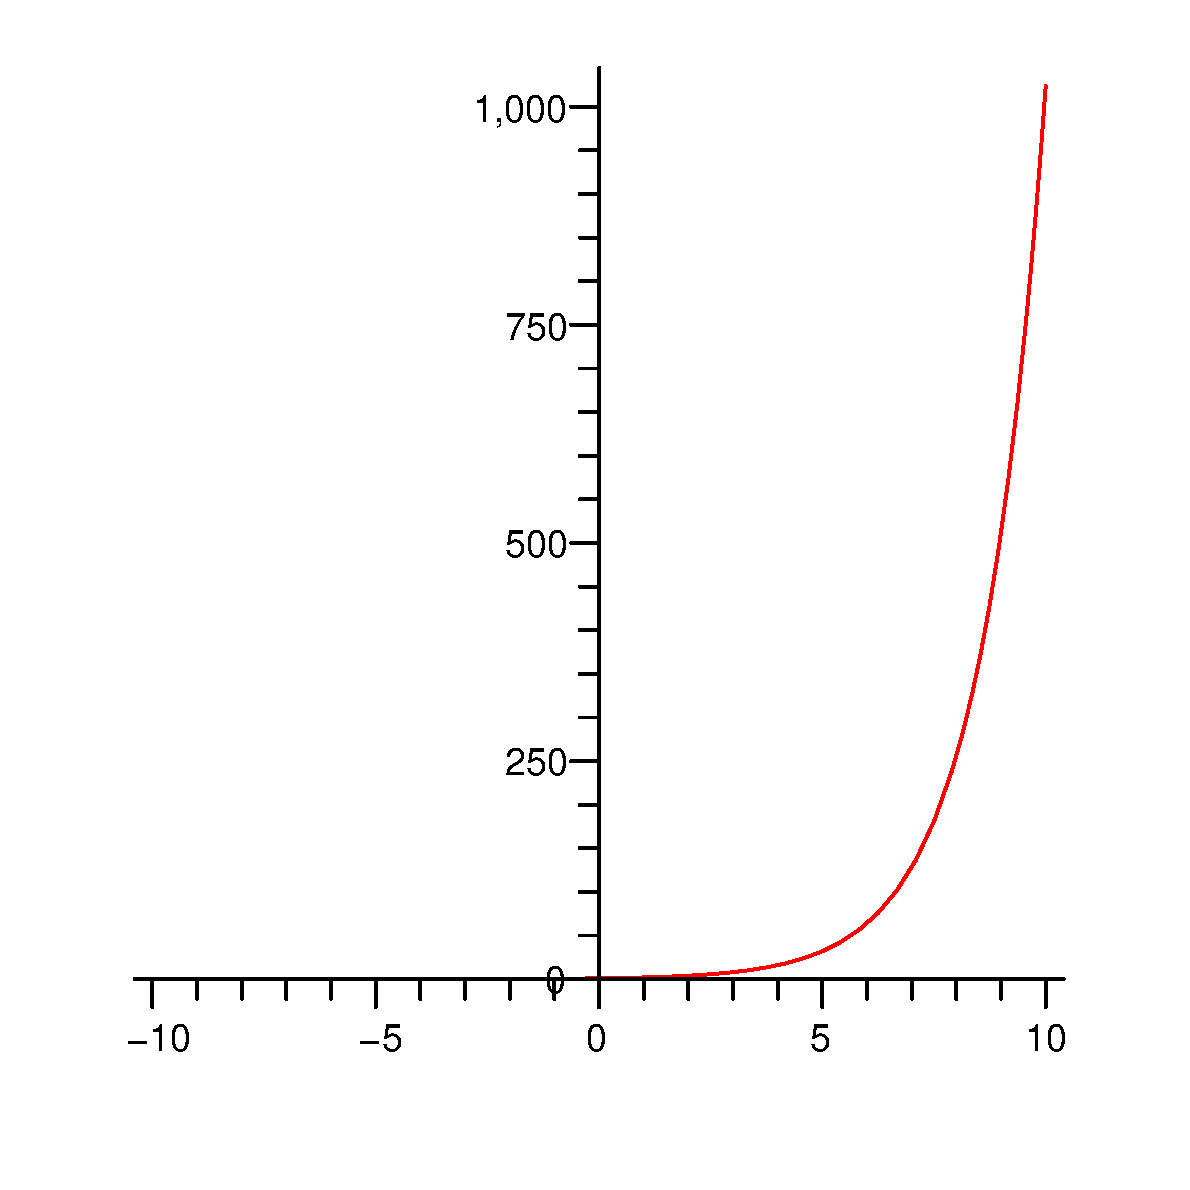
\includegraphics[height=3.39cm]{547.eps}
% napperon.eps : 300dpi, width=3.39cm, height=3.39cm, bb=0 0 400 400
    \end{center}
La r\'eponse est donc b).\\

548-- Parmi les quatre choix ci-dessous, lequel compl\`ete
correctement l'\'enonc\'e suivant : \og Une base positive affect\'ee
d'un exposant entier ou fractionnaire correspond \`a une valeur r\'eelle appel\'ee $\ldots$\fg ?\\
a) multiplication.\\
b) produit.\\
c) puissance.\\
d) somme.\\

R\'eponse : c)\\

R\'etroaction : \\
Une base positive affect\'ee d'un exposant entier ou fractionnaire
correspond \`a une valeur r\'eelle appel\'ee puissance.  La r\'eponse est
c).\\

549-- La temp\'erature d'une soupe d\'ecro\^it  exponentiellement selon le
temps \'ecoul\'e.  Parmi les choix suivants, lequel est vrai?\\
a) La temp\'erature de la soupe d\'ecro\^it lentement au d\'ebut, rapidement
par la suite et de nouveau lentement.\\
b) La temp\'erature de la soupe d\'ecro\^it lentement au d\'ebut et
rapidement par la suite.\\
c) La temp\'erature de la soupe d\'ecro\^it rapidement au d\'ebut et
lentement par la suite.  \\
d) La temp\'erature de la soupe d\'ecro\^it rapidement au d\'ebut, lentement
par la suite et de nouveau rapidement.\\

R\'eponse : c)\\

R\'etroaction : \\
La temp\'erature de la soupe d\'ecro\^it rapidement au d\'ebut et lentement
par la suite.  La r\'eponse est c).\\

550-- Parmi les quatre \'equations suivantes, laquelle est une droite?\\
a) $y=4^{x}$\\[2mm]
b) $y=\frac{3x}{5}-1$\\[2mm]
c) $y=\frac{3x^{2}}{5}-1$\\[2mm]
d) $y=x^{4}$\\

R\'eponse : b)\\

R\'etroaction : \\
L'\'equation $y=\frac{3x}{5}-1$ est une droite, dont voici le
graphique : \\
    \begin{center}
    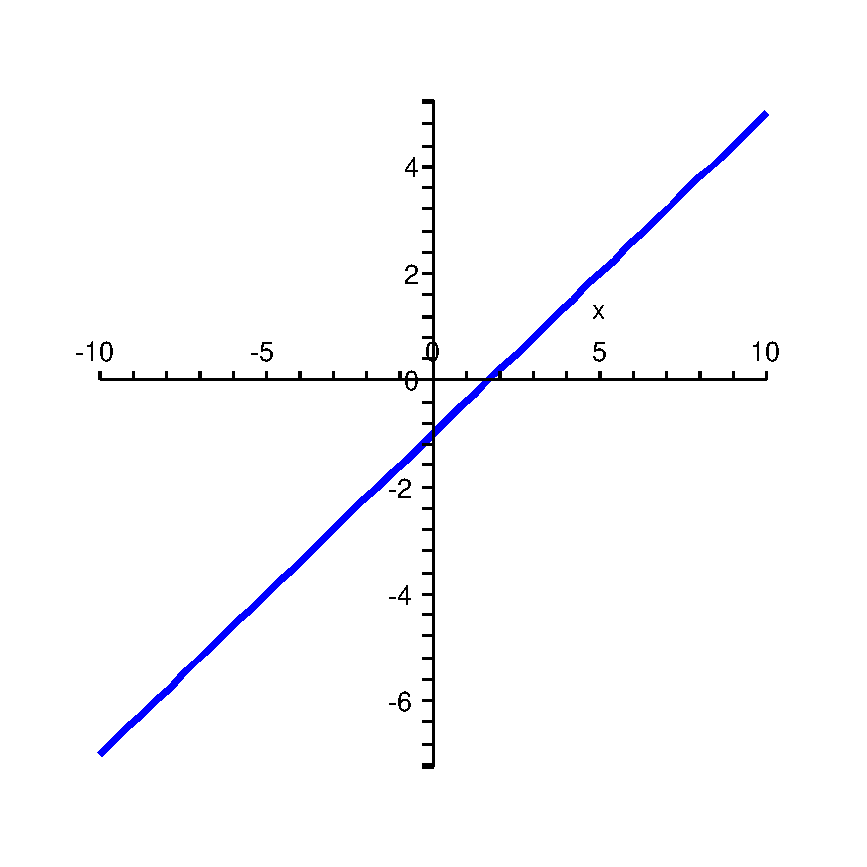
\includegraphics[width=6cm,bb=0 0 400 400]{fonction20.eps}
% fonction20.eps : 300dpi, width=3.39cm, height=3.39cm, bb=0 0 400 400
    \end{center}

La r\'eponse est b).\\


552-- Si $x$ est la variable ind\'ependante et $y$ la variable d\'ependante,
quelle est l'abscisse du point d'intersection des droites $y=4x-9$ et
$y=2x-5$?\\

R\'eponse : 2\\

R\'etroaction : \\
Comme la valeur de $y$ au point d'intersection est la m\^eme pour les deux
droites, on peut \'ecrire:\\
$4x-9=2x-5$\\
$2x-9=-5$\\
$2x=4$\\
$x=2$\\

Les deux droites se croisent en $x=2$.\\

553-- Si $x$ est la variable ind\'ependante et $y$ la variable d\'ependante,
quelle est l'abscisse du point d'intersection des droites $y=2x-3$ et
$y=-3x-8$?\\

R\'eponse : $-1$\\

R\'etroaction : \\
Comme la valeur de $y$ au point d'intersection est la m\^eme pour les deux
droites, on peut \'ecrire:\\
$2x-3=-3x-8$\\
$5x-3=-8$\\
$5x=-5$\\
$x=-1$\\

Les deux droites se croisent en $x=-1$.\\

554-- Si $x$ est la variable ind\'ependante et $y$ la variable d\'ependante,
quelle est l'abscisse du point d'intersection des droites $2y\,+\,2x-3=0$ et
$2y=-3x-8$?\\

R\'eponse : $-11$\\

R\'etroaction : \\
On a les \'equations suivantes:\\
$2y\,+\,2x-3=0  \qquad $(\'equation 1),\\
$2y=-3x-8  \qquad $(\'equation 2).\\

On remplace $2y$ de l'\'equation 1 par sa valeur obtenue dans l'\'equation
2.\\
$2y\,+\,2x-3=0$\\
$-3x-8\,+\,2x-3=0$\\
$-x-8-3=0$\\
$-x-11=0$\\
$-x=11$\\
$x=-11$\\
Les deux droites se croisent en $x=-11$.\\

555-- Si $x$ est la variable ind\'ependante et $y$ la variable d\'ependante,
quelle est l'abscisse du point d'intersection des droites
$4y\,+\,2x\,+\,7=0$ et $4y-3x-8=0$?\\

R\'eponse : $-3$\\

R\'etroaction : \\
Il faut commencer par isoler le $4y$ dans une des deux \'equations, disons
la premi\`ere.\\
$4y\,+\,2x\,+\,7=0$\\
$4y=-7-2x$\\

Il faut maintenant substituer $4y$ par sa valeur dans $4y-3x-8=0$.\\
$4y-3x-8=0$\\
$-7-2x-3x-8=0$\\
$-5x-7-8=0$\\
$-5x-15=0$\\
$-5x=15$\\
$x=-3$\\
Les deux droites se croisent en $x=-3$.\\

556-- Dans un plan cart\'esien, combien de points d'intersection deux
droites non confondues ayant la m\^eme pente ont-elles?\\

R\'eponse : 0\\

R\'etroaction :\\
Deux droites ayant la m\^eme pente sont parall\`eles et ne se couperont donc
jamais.  Par cons\'equent, elles n'ont aucun point en commun.  Voici un
exemple de deux droites de m\^eme pente.\\
    \begin{center}
    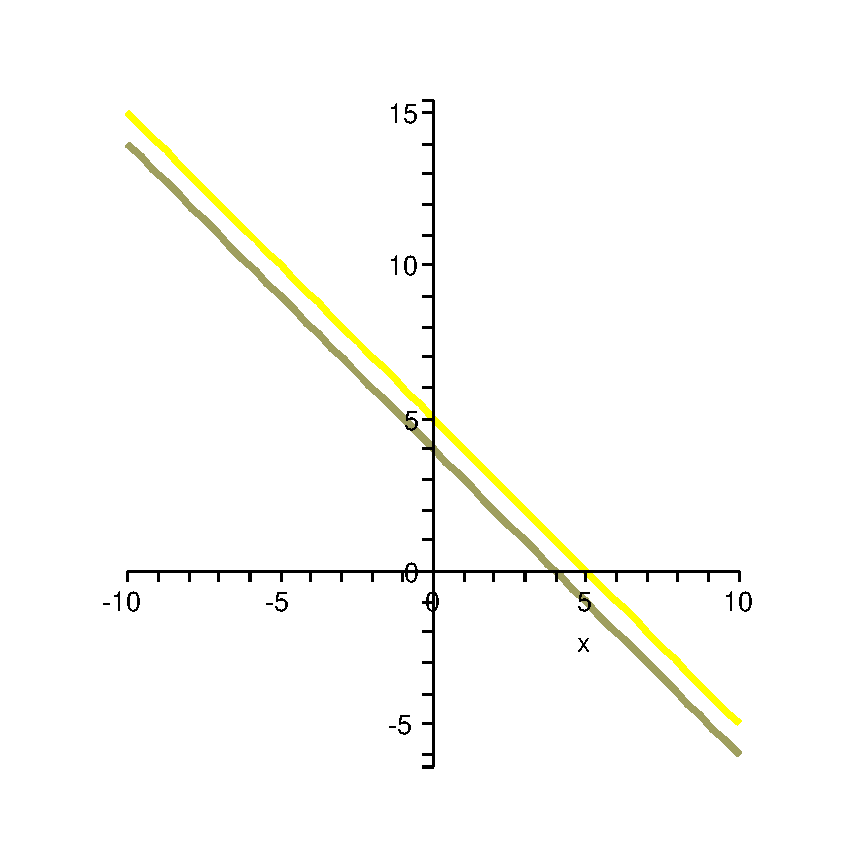
\includegraphics[width=6cm,bb=0 0 400 400]{fonction21.eps}
% fonction21.eps : 300dpi, width=3.39cm, height=3.39cm, bb=0 0 400 400
    \end{center}

La r\'eponse est 0.\\



557-- Parmi les quatre choix ci-dessous, lequel donne le nombre de points
d'intersection de deux droites confondues?\\
a) 0\\
b) 1\\
c) 10\\
d) Une infinit\'e\\

R\'eponse : d)\\

R\'etroaction : \\
Deux droites confondues sont l'une sur l'autre.  Elles ont donc une
infinit\'e de points en commun.  La r\'eponse est d).\\

558-- Dans un triangle rectangle, lequel des rapports suivants permet de
trouver le cosinus d'un angle?\\[2mm]
a) $\frac{\textrm{mesure du c\^ot\'e adjacent}}{\textrm{mesure de
l'hypot\'enuse}}$\\[2mm]
b) $\frac{\textrm{mesure du c\^ot\'e oppos\'e}}{\textrm{mesure du c\^ot\'e
adjacent}}$\\[2mm]
c) $\frac{\textrm{mesure du c\^ot\'e oppos\'e}}{\textrm{mesure de
l'hypot\'enuse}}$\\[2mm]
d) $\frac{\textrm{mesure de l'hypot\'enuse}}{\textrm{mesure du c\^ot\'e
adjacent}}$\\

R\'eponse : a)\\

R\'etroaction : \\
Cosinus d'un angle = $\frac{\textrm{mesure du c\^ot\'e
adjacent}}{\textrm{mesure de l'hypot\'enuse}}$\\[2mm]
Tangente d'un angle = $\frac{\textrm{mesure du c\^ot\'e
oppos\'e}}{\textrm{mesure du c\^ot\'e adjacent}}$\\[2mm]
Sinus d'un angle = $\frac{\textrm{mesure du c\^ot\'e
oppos\'e}}{\textrm{mesure de l'hypot\'enuse}}$\\[2mm]
S\'ecante d'un angle =  $\frac{\textrm{mesure de
l'hypot\'enuse}}{\textrm{mesure du c\^ot\'e adjacent}}$\\[2mm]
La r\'eponse est a).\\

559-- Dans un triangle rectangle, lequel des rapports suivants permet de
trouver le sinus d'un angle?\\[2mm]
a) $\frac{\textrm{mesure du c\^ot\'e adjacent}}{\textrm{mesure de
l'hypot\'enuse}}$\\[2mm]
b) $\frac{\textrm{mesure du c\^ot\'e oppos\'e}}{\textrm{mesure du c\^ot\'e
adjacent}}$\\[2mm]
c) $\frac{\textrm{mesure du c\^ot\'e oppos\'e}}{\textrm{mesure de
l'hypot\'enuse}}$\\[2mm]
d) $\frac{\textrm{mesure de l'hypot\'enuse}}{\textrm{mesure du c\^ot\'e
adjacent}}$\\

R\'eponse : c)\\

R\'etroaction : \\
Cosinus d'un angle = $\frac{\textrm{mesure du c\^ot\'e
adjacent}}{\textrm{mesure de l'hypot\'enuse}}$\\[2mm]
Tangente d'un angle = $\frac{\textrm{mesure du c\^ot\'e
oppos\'e}}{\textrm{mesure du c\^ot\'e adjacent}}$\\[2mm]
Sinus d'un angle = $\frac{\textrm{mesure du c\^ot\'e
oppos\'e}}{\textrm{mesure de l'hypot\'enuse}}$\\[2mm]
S\'ecante d'un angle =  $\frac{\textrm{mesure de
l'hypot\'enuse}}{\textrm{mesure du c\^ot\'e adjacent}}$\\[2mm]
La r\'eponse est donc c).\\

560-- Dans un triangle rectangle ABC, le segment BC mesure 4\,cm, le segment
BA, 5\,cm et le segment AC, 3\,cm.  L'angle droit est en C.  Parmi les
quatre choix ci-dessous, lequel repr\'esente le nom du rapport $\frac{4}{3}$
par rapport \`a l'angle A?\\
a) Cosinus de l'angle A\\
b) Cotangente de l'angle A\\
c) Sinus de l'angle A\\
d) Tangente de l'angle A\\

R\'eponse : d)

R\'etroaction : \\
Tangente de l'angle A = $\frac{\textrm{mesure du c\^ot\'e
oppos\'e}}{\textrm{mesure du c\^ot\'e
adjacent}}\,=\,\frac{\textrm{4}}{\textrm{3}}$\\
    \begin{center}
    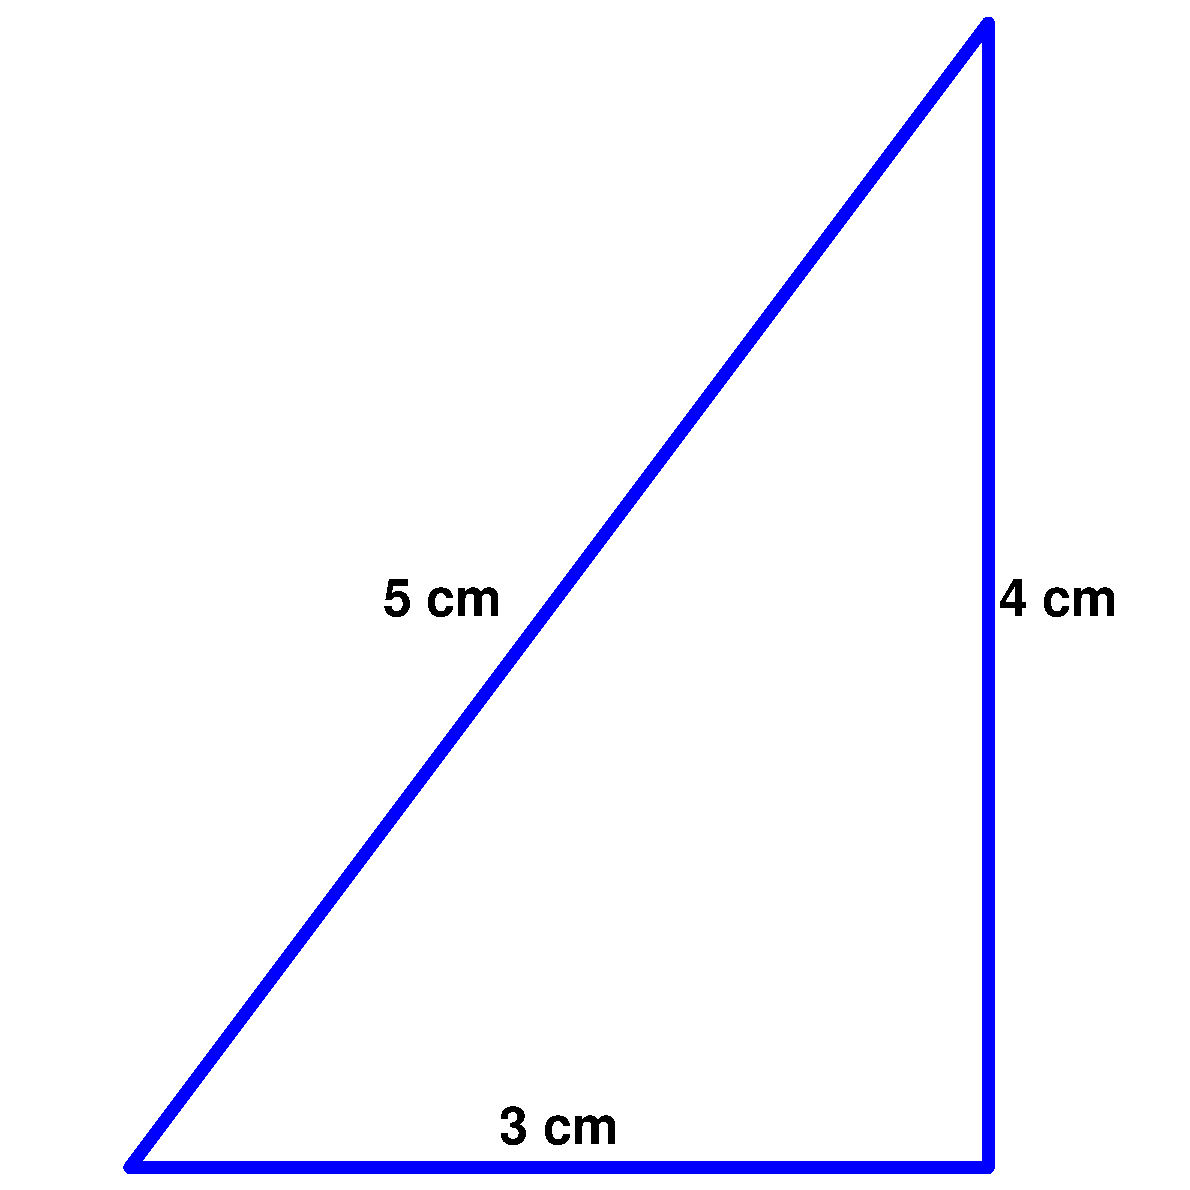
\includegraphics[width=4.5cm]{triangle21.eps}
% triangle21.eps : 300dpi, width=3.39cm, height=3.39cm, bb=0 0 400 400
    \end{center}

La r\'eponse est d).\\


562-- Dans un triangle rectangle ABC, le segment BC mesure 4\,cm, le segment
BA, 5\,cm et le segment AC, 3\,cm.  L'angle droit est en C.  Parmi les
quatre choix ci-dessous, lequel repr\'esente le nom du rapport $\frac{3}{5}$
par rapport \`a l'angle A?\\
a) Cosinus de l'angle A\\
b) Cotangente de l'angle A\\
c) Sinus de l'angle A\\
d) Tangente de l'angle A\\

R\'eponse : a)

R\'etroaction : \\
Cosinus de l'angle A = $\frac{\textrm{mesure du c\^ot\'e
adjacent}}{\textrm{mesure de
l'hypot\'enuse}}\,=\,\frac{\textrm{3}}{\textrm{5}}$\\
\begin{center}
    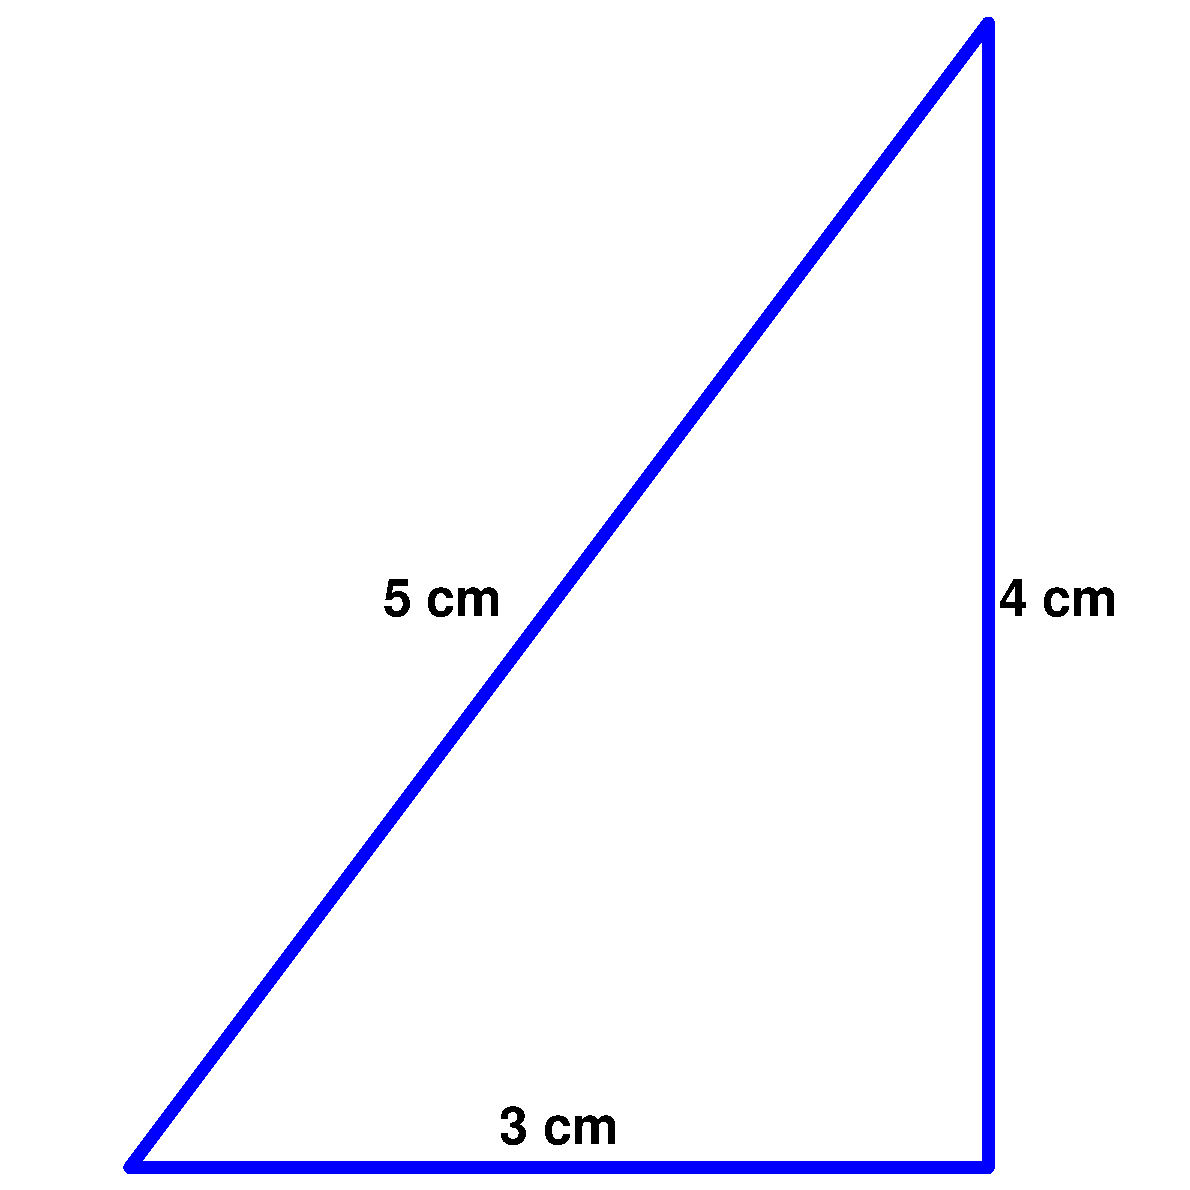
\includegraphics[width=4.5cm]{triangle21.eps}
% triangle21.eps : 300dpi, width=3.39cm, height=3.39cm, bb=0 0 400 400
    \end{center}
La r\'eponse est a).\\

563-- Dans un triangle rectangle ABC, le segment BC mesure 4\,cm, le segment
BA, 5\,cm et le segment AC, 3\,cm.  L'angle droit est en C.  Parmi les
quatre choix ci-dessous, lequel repr\'esente le nom du rapport $\frac{3}{4}$
par rapport \`a l'angle B?\\
a) Cosinus de l'angle B\\
b) Cotangente de l'angle B\\
c) Sinus de l'angle B\\
d) Tangente de l'angle B\\

R\'eponse : d)

R\'etroaction : \\
Tangente de l'angle B = $\frac{\textrm{mesure du c\^ot\'e
oppos\'e}}{\textrm{mesure du c\^ot\'e
adjacent}}\,=\,\frac{\textrm{3}}{\textrm{4}}$\\
\begin{center}
    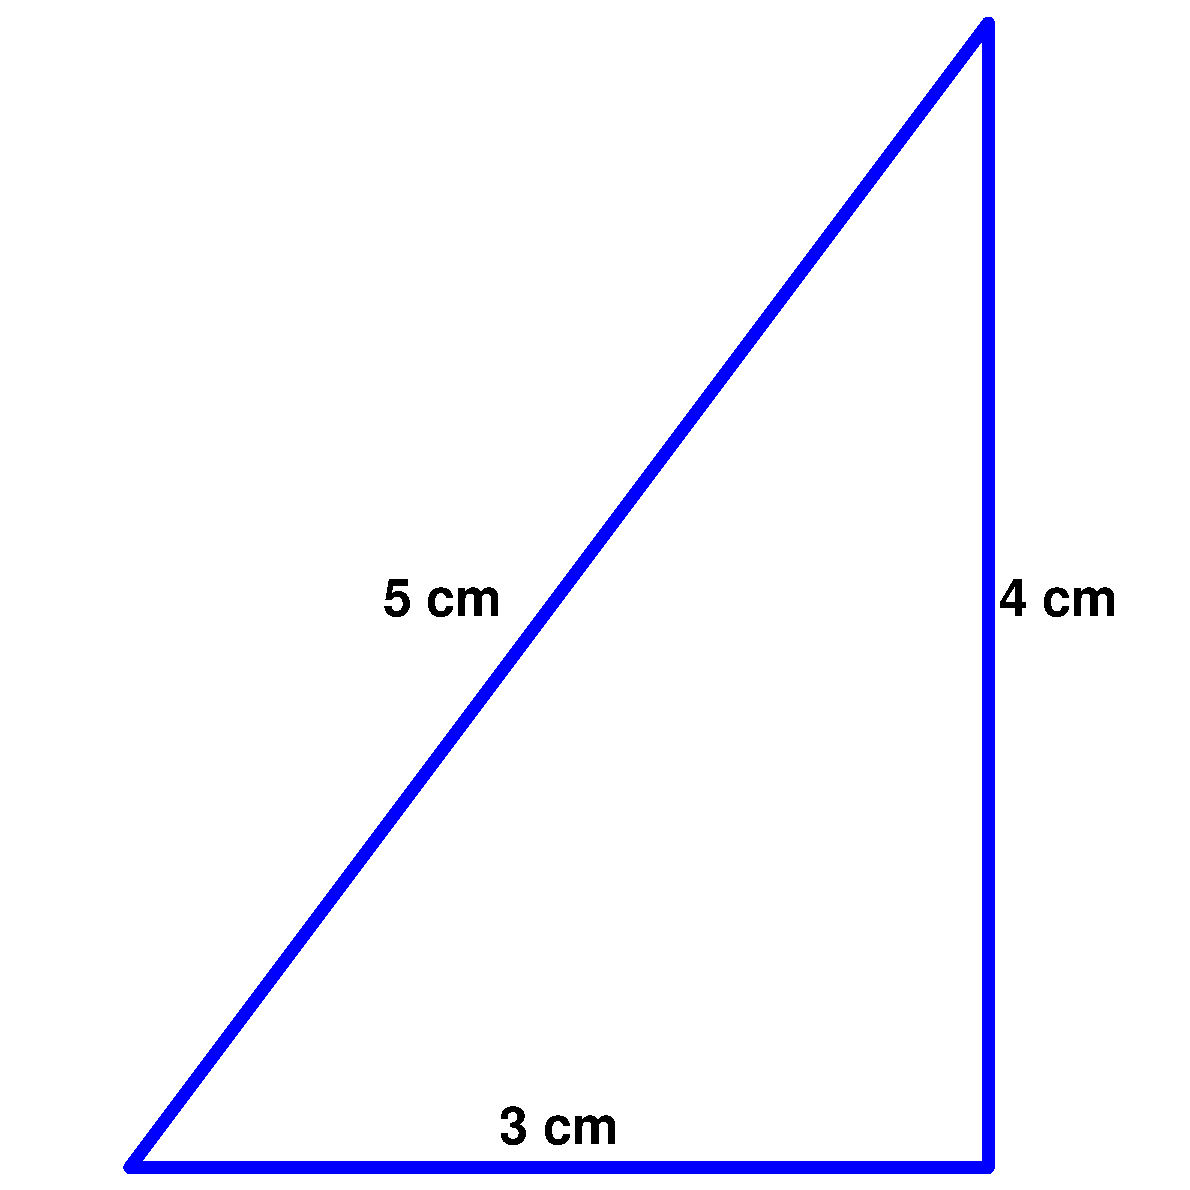
\includegraphics[width=4.5cm]{triangle21.eps}
% triangle21.eps : 300dpi, width=3.39cm, height=3.39cm, bb=0 0 400 400
    \end{center}
La r\'eponse est d).\\

564-- Dans un triangle rectangle ABC, le segment BC mesure 4\,cm, le segment
BA, 5\,cm et le segment AC, 3\,cm.  L'angle droit est en C.  Parmi les
quatre choix ci-dessous, lequel repr\'esente le nom du rapport $\frac{3}{5}$
par rapport \`a l'angle B?\\
a) Cosinus de l'angle B\\
b) Cotangente de l'angle B\\
c) Sinus de l'angle B\\
d) Tangente de l'angle B\\

R\'eponse : c)

R\'etroaction : \\
Sinus de l'angle B = $\frac{\textrm{mesure du c\^ot\'e
oppos\'e}}{\textrm{mesure de
l'hypot\'enuse}}\,=\,\frac{\textrm{3}}{\textrm{5}}$\\
\begin{center}
    \includegraphics[width=4.5cm]{triangle21.eps}
% triangle21.eps : 300dpi, width=3.39cm, height=3.39cm, bb=0 0 400 400
    \end{center}
La r\'eponse est c).\\

565-- Dans un triangle rectangle ABC, le segment BC mesure 4\,cm, le segment
BA, 5\,cm et le segment AC, 3\,cm.  L'angle droit est en C.  Parmi les
quatre choix ci-dessous, lequel repr\'esente le nom du rapport $\frac{4}{5}$
par rapport \`a l'angle B?\\
a) Cosinus de l'angle B\\
b) Cotangente de l'angle B\\
c) Sinus de l'angle B\\
d) Tangente de l'angle B\\

R\'eponse : a)

R\'etroaction : \\
Cosinus de l'angle B = $\frac{\textrm{mesure du c\^ot\'e
adjacent}}{\textrm{mesure de
l'hypot\'enuse}}\,=\,\frac{\textrm{4}}{\textrm{5}}$\\
\begin{center}
    \includegraphics[width=4.5cm]{triangle21.eps}
% triangle21.eps : 300dpi, width=3.39cm, height=3.39cm, bb=0 0 400 400
    \end{center}
La r\'eponse est a).\\

566-- Le sinus d'un angle est 1.  Parmi les quatre choix suivants, lequel
donne la mesure de cet angle?\\
a) 30$^{\circ}$\\
b) 60$^{\circ}$\\
c) 90$^{\circ}$\\
d) 180$^{\circ}$\\

R\'eponse : c)\\

R\'etroaction : \\
$\arcsin 1 = 90^{\circ}$\\
La r\'eponse est donc c).\\

567-- Le cosinus d'un angle est 0.  Parmi les quatre choix suivants, lequel
donne la mesure de cet angle?\\
a) 30$^{\circ}$\\
b) 60$^{\circ}$\\
c) 90$^{\circ}$\\
d) 180$^{\circ}$\\

R\'eponse : c)\\

R\'etroaction : \\
$\arccos 0 = 90^{\circ}$\\
La r\'eponse est donc c).\\

568-- La tangente d'un angle est 1.  Parmi les quatre choix suivants, lequel
donne la mesure de cet angle?\\
a) 45$^{\circ}$\\
b) 60$^{\circ}$\\
c) 90$^{\circ}$\\
d) 180$^{\circ}$\\

R\'eponse : a)\\

R\'etroaction : \\
$\arctan 1 = 45^{\circ}$\\
La r\'eponse est donc a).\\

569-- Le sinus d'un angle est 0.  Parmi les quatre choix suivants, lequel
donne la mesure de cet angle?\\
a) 0$^{\circ}$\\
b) 30$^{\circ}$\\
c) 60$^{\circ}$\\
d) 90$^{\circ}$\\

R\'eponse : a)\\

R\'etroaction : \\
$\arcsin 0 = 0^{\circ}$\\
Par cons\'equent, la r\'eponse est a).\\

570-- \`A une distance de 20 m, l'angle d'\'el\'evation du sommet d'un
\'edifice est 63$^{\circ}$. Quelle est la hauteur de cet ?ifice?\\

R\'eponse : 39  \\

R\'etroaction : \\
Soit x la hauteur de l'\'edifice.\\[2mm]   \begin{center}
    \includegraphics[height=3.39cm]{570.eps}
% napperon.eps : 300dpi, width=3.39cm, height=3.39cm, bb=0 0 400 400
    \end{center}
$\frac{x}{20}=\tan 63^{\circ}$\\[2mm]
$\frac{x}{20}=1,9626105$\\[2mm]
$x=1,9626105\times20=39,25$\\[2mm]
Il faut maintenant arrondir \`a l'unit\'e.
La r\'eponse est 39 m.\\



572-- Un triangle quelconque dont les c\^ot\'es mesurent $a$, $b$ et $c$
unit\'es a un p\'erim\`etre \'egal \`a $2p$ unit\'es.  Parmi les quatre
\'equations suivantes, laquelle repr\'esente la formule de H\'eron?\\
a) Aire du triangle = $\sqrt{p\left( a-p\right) \left( b-p\right) \left(
c-p\right) }$\\[2mm]
b) Aire du triangle = $\sqrt{p\left( a-b\right) \left( b-c\right) \left(
c-p\right) }$\\[2mm]
c) Aire du triangle = $\sqrt{p\left( b-p\right) \left( b-c\right) \left(
c-p\right) }$\\[2mm]
d) Aire du triangle = $\sqrt{p\left( p-a\right) \left( p-b\right) \left(
p-c\right) }$\\

R\'eponse : d)\\

R\'etroaction : \\
La formule de H\'eron est donn\'ee par l'expression suivante:\\
aire du triangle = $\sqrt{p\left( p-a\right) \left( p-b\right) \left(
p-c\right) }$.  La r\'eponse est d).\\

573-- Parmi les choix suivants, que permet de calculer la formule de
H\'eron?\\
a) Aire d'un hexagone\\
b) Aire d'un octogone\\
c) Aire d'un pentagone\\
d) Aire d'un triangle\\

R\'eponse : d) \\

R\'etroaction : \\
La formule de H\'eron permet de calculer l'aire d'un triangle.  Par
cons\'equent, la r\'eponse est d).\\



574-- Parmi les quatre choix ci-dessous, lequel compl\`ete
correctement l'\'enonc\'e suivant : \og Deux figures isom\'etriques
ayant tous leurs \'el\'ements homologues congrus sont parfaitement $\ldots$\fg ?\\
a) de la m\^eme couleur.\\
b) inversibles.\\
c) r\'eversibles.\\
d) superposables.\\

R\'eponse : d)\\

R\'etroaction : \\
Deux figures isom\'etriques ayant tous leurs \'el\'ements homologues congrus
sont parfaitement superposables.  La r\'eponse est d).\\

575-- De combien de fa\c cons peut-on couper un carr\'e en deux pour obtenir
deux figures isom\'etriques?\\

R\'eponse : 4\\

R\'etroaction : \\
Il y a quatre fa\c cons possibles :   \\
    \begin{center}
    \includegraphics[width=6cm,bb=0 0 400 400]{quatrecarres.eps}
% quatrecarres.eps : 300dpi, width=3.39cm, height=3.39cm, bb=0 0 400 400
    \end{center}


576-- De combien de fa\c cons peut-on couper un triangle \'equilat\'eral
pour obtenir deux triangles congrus?\\

R\'eponse : 3\\

R\'etroaction\\
En tra\c cant la m\'ediatrice de chaque segment, on obtient trois mani\`eres
diff\'erentes de cr\'eer deux triangles congrus.  Les voici :\\
    \begin{center}
    \includegraphics[width=6cm,bb=0 0 400 400]{troistriangles.eps}
% troistriangles.eps : 300dpi, width=3.39cm, height=3.39cm, bb=0 0 400 400
    \end{center}


577-- Parmi les quatre choix suivants, lequel repr\'esente le nombre de
droites globalement invariantes lors d'une sym\'etrie gliss\'ee?\\
a) 0\\
b) 1\\
c) 2\\
d) Une infinit\'e\\

R\'eponse : b)\\

R\'etroaction : \\
La seule droite globalement invariante lors d'une sym\'etrie gliss\'ee est
l'axe de r\'eflexion.  La r\'eponse est donc b).\\

578-- Parmi les quatre choix suivants, lequel repr\'esente le nombre de
points fixes dans une rotation?\\
a) 0\\
b) 1\\
c) 2\\
d) Une infinit\'e\\

R\'eponse : b)\\

R\'etroaction : \\
Dans une rotation, le seul point fixe est le centre de rotation.  La
r\'eponse est donc b).\\

579-- Parmi les quatre choix suivants, lequel repr\'esente le nombre de
points fixes dans une translation?\\
a) 0 \\
b) 1\\
c) 3\\
d) Une infinit\'e\\

R\'eponse : a)\\

R\'etroaction : \\
Dans une translation, il n'y a aucun point fixe, \`a moins que la
translation soit l'identit\'e.  La r\'eponse est a).\\

580-- On trace la diagonale d'un carr\'e, cr\'eant ainsi deux
triangles rectangles congrus.\\
\begin{center}
    \includegraphics[height=3.39cm]{580.eps}
% napperon.eps : 300dpi, width=3.39cm, height=3.39cm, bb=0 0 400 400
    \end{center}
Parmi les quatre choix ci-dessous, lequel repr\'esente
les isom\'etries qui associent un triangle \`a l'autre?\\
a) R\'eflexion et rotation\\
b) Rotation et sym\'etrie gliss\'ee\\
c) Sym\'etrie gliss\'ee et translation\\
d) Translation et rotation\\

R\'eponse : a) \\

R\'etroaction : \\
L'isom\'etrie qui associe un triangle \`a l'autre est la r\'eflexion.  La
r\'eponse est a).\\


582-- Parmi les quatre choix suivants, lequel est \'equivalent \`a
$t_{\left(4,\,3\right)} \circ t_{\left(2,\,6\right) }$?\\
a) $t_{\left(2,\,-3\right) }$\\
b) $t_{\left(6,\,9\right) }$\\
c) $t_{\left(7,\,5\right) }$\\
d) $t_{\left(9,\,6\right) }$\\

R\'eponse : b)\\

R\'etroaction : \\
$t_{\left(4,\,3\right)} \circ t_{\left(2,\,6\right) }= t_{\left(6,\,9\right)
}$\\
La r\'eponse est b).\\

583-- Parmi les quatre choix suivants, lequel est \'equivalent \`a
$t_{\left(a,\,b\right)} \circ t_{\left(c,\,d\right) }$?\\
a) $t_{\left(a\,+\,b,\,c\,+\,d\right) }$\\
b) $t_{\left(a\,+\,c,\,b\,+\,d\right) }$\\
c) $t_{\left(a\,+\,d,\,b\,+\,c\right) }$\\
d) $t_{\left(b\,+\,c,\,a\,+\,d\right) }$\\

R\'eponse : b)\\

R\'etroaction : \\
$t_{\left(a,\,b\right)} \circ t_{\left(c,\,d\right)
}=t_{\left(a\,+\,c,\,b\,+\,d\right) }$\\
La r\'eponse est b).\\

584-- Parmi les quatre choix suivants, lequel est \'equivalent \`a
$r_{\left( O,\,\,90^{\circ}\right)} \circ r_{\left( O,\,\,95^{\circ}\right)
}$?\\
a) $r_{\left(O,\,-5^{\circ}\right) }$\\
b) $r_{\left(O,\,5^{\circ}\right) }$\\
c) $r_{\left(O,\,-185^{\circ}\right) }$\\
d) $r_{\left(O,\,185^{\circ}\right) }$\\

R\'eponse : d)\\

R\'etroaction : \\
Comme les deux rotations sont de m\^eme centre, il suffit d'additionner les
angles de rotation.\\
$90^{\circ}\,+\,95^{\circ}=185^{\circ}$\\
Par cons\'equent, la r\'eponse est d).\\

585-- Parmi les quatre choix ci-dessous, lequel est \'equivalent \`a $r\circ
t$?\\
a) R\'eflexion\\
b) Rotation\\
c) Sym\'etrie gliss\'ee\\
d) Translation\\

R\'eponse : b) \\

R\'etroaction : \\
La compos\'ee d'isom\'etries $r\circ t$ est \'equivalente \`a une
rotation.\\
La r\'eponse est b).\\

586-- Parmi les quatre choix ci-dessous, lequel est \'equivalent \`a une
r\'eflexion compos\'ee \`a une autre r\'eflexion, si les deux axes de
r\'eflexion ne sont pas parall\`eles?\\
a) R\'eflexion\\
b) Rotation\\
c) Sym\'etrie gliss\'ee\\
d) Translation\\

R\'eponse : b) \\

R\'etroaction : \\
Si les deux axes de r\'eflexion ne sont pas parall\`eles, la compos\'ee de
deux r\'eflexions est une rotation.\\
La r\'eponse est b).\\

587-- Parmi les quatre choix ci-dessous, lequel est \'equivalent \`a une
r\'eflexion compos\'ee \`a une autre r\'eflexion, si les deux axes de
r\'eflexion sont parall\`eles?\\
a) R\'eflexion\\
b) Rotation\\
c) Sym\'etrie gliss\'ee\\
d) Translation\\

R\'eponse : d) \\

R\'etroaction : \\
Si les deux axes de r\'eflexion sont parall\`eles, la compos\'ee de deux
r\'eflexions est une translation.\\
La r\'eponse est d).\\

588-- Parmi les quatre choix ci-dessous, lequel est \'equivalent \`a
$r_{\left(A,\,75^{\circ}\right)} \circ r_{\left(B,\,-75^{\circ}\right) }$,
si $A\neq B$?\\
a) R\'eflexion\\
b) Rotation\\
c) Sym\'etrie gliss\'ee\\
d) Translation\\

R\'eponse : d)\\

R\'etroaction : \\
La compos\'ee $r_{\left(A,\,75^{\circ}\right)} \circ
r_{\left(B,\,-75^{\circ}\right) }$ est \'equivalente \`a une translation, si
$A\neq B$.  La r\'eponse est d).\\

589-- Parmi les quatre choix ci-dessous, lequel est \'equivalent \`a une
translation suivie d'une r\'eflexion, si la fl\`eche de translation n'est
pas perpendiculaire \`a l'axe de r\'eflexion?\\
a) R\'eflexion\\
b) Rotation\\
c) Sym\'etrie gliss\'ee\\
d) Translation\\

R\'eponse : c)\\

R\'etroaction : \\
Si la fl\`eche de translation n'est pas perpendiculaire \`a l'axe de
r\'eflexion, une translation suivie d'une r\'eflexion  \'equivaut \`a une
sym\'etrie gliss\'ee.  La r\'eponse est c).\\

590-- Une compos\'ee d'isom\'etries est une identit\'e si, apr\`es la
composition, la figure image est la figure initiale elle-m\^eme.  Parmi les
quatre compos\'ees d'isom\'etries suivantes, laquelle est une identit\'e?\\
a) $t_{\left(1,\,2\right) } \circ t_{\left(-1,\,-2\right) } $\\
b) $r_{\left(O,\,90^{\circ}\right)} \circ r_{\left(O,\,180^{\circ}\right)}
$\\
c) $r_{\left(O,\,180^{\circ}\right)} \circ r_{\left(O,\,-90^{\circ}\right)}
$\\
d) $r_{\left(O,\,180^{\circ}\right)} \circ t_{\left(0,\,-180\right)} $   \\

R\'eponse : a) \\

R\'etroaction : \\
La compos\'ee $t_{\left(1,\,2\right) } \circ t_{\left(-1,\,-2\right) } $ est
une identit\'e.  La r\'eponse est a).\\


592--  Parmi les quatre expressions ci-dessous, laquelle compl\`ete
correctement l'\'enonc\'e suivant : \og Une conjecture qui s'av\`ere
exacte suite \`a une preuve s'appelle $\dots$\fg ?\\
a) un \'enonc\'e.\\
b) une phrase. \\
c) un th\'eor\`eme.\\
d) une validation.\\

R\'eponse : c)\\

R\'etroaction : \\
Une conjecture qui s'av\`ere exacte suite \`a une preuve s'appelle un
th\'eor\`eme.  La r\'eponse est c).\\

593-- Parmi les quatre expressions ci-dessous, laquelle compl\`ete
correctement l'\'enonc\'e suivant : \og Un \'enonc\'e qui semble
vrai, mais qui n'a pas encore \'et\'e prouv\'e est $\ldots$\fg ?\\
a) un axiome.\\
b) une conjecture.\\
c) un th\'eor\`eme.\\
d) une validation.\\

R\'eponse : b)\\

R\'etroaction : \\
Un \'enonc\'e qui semble vrai, mais qui n'a pas encore \'et\'e prouv\'e est
une conjecture.  La r\'eponse est b).\\

594-- Parmi les expressions ci-dessous, laquelle compl\`ete
correctement l'\'enonc\'e suivant : \og Un \'enonc\'e qui est
 accept\'e sans preuve est $\ldots$\fg ?\\
a) un axiome.\\
b) une conjecture.\\
c) un fait.\\
d) un th\'eor\`eme.\\

R\'eponse : a)\\

R\'etroaction : \\
Un \'enonc\'e qui est accept\'e sans preuve est un
axiome.  La r\'eponse est a).  \\

595-- Parmi les quatre \'enonc\'es suivants, lequel est vrai?\\
a) Deux angles alternes-internes form\'es par deux droites parall\`eles et
une s\'ecante \`a ces deux droites sont congrus.\\
b) Deux angles alternes-internes form\'es par deux droites non parall\`eles
et une s\'ecante \`a ces deux droites sont congrus.\\
c) Deux angles alternes-internes form\'es par deux droites parall\`eles et
une s\'ecante \`a ces deux droites ne sont pas congrus.\\
d) Deux angles alternes-internes form\'es par deux droites non parall\`eles
et une s\'ecante \`a une de ces deux droites sont congrus.\\

R\'eponse : a)\\

R\'etroaction : \\
Deux angles alternes-internes form\'es par deux droites parall\`eles
et une s\'ecante \`a ces deux droites sont congrus.   \begin{center}
    \includegraphics[height=3.39cm]{595.eps}
% napperon.eps : 300dpi, width=3.39cm, height=3.39cm, bb=0 0 400 400
    \end{center}  La r\'eponse est a).\\

596-- Parmi les quatre \'enonc\'es suivants, lequel est vrai?\\
a) Deux angles alternes-externes form\'es par deux droites parall\`eles et
une s\'ecante \`a ces deux droites sont congrus.\\
b) Deux angles alternes-externes form\'es par deux droites non parall\`eles
et une s\'ecante \`a ces deux droites sont congrus.\\
c) Deux angles alternes-externes form\'es par deux droites parall\`eles et
une s\'ecante \`a ces deux droites ne sont pas congrus.\\
d) Deux angles alternes-externes form\'es par deux droites non parall\`eles
et une s\'ecante \`a une de ces deux droites sont congrus.\\

R\'eponse : a)\\

R\'etroaction : \\
Deux angles alternes-externes form\'es par deux droites parall\`eles
et une s\'ecante \`a ces deux droites sont congrus.   \begin{center}
    \includegraphics[height=3.39cm]{596.eps}
% napperon.eps : 300dpi, width=3.39cm, height=3.39cm, bb=0 0 400 400
    \end{center}  La r\'eponse est a).\\

597-- Parmi les quatre \'enonc\'es suivants, lequel est vrai?\\
a) Deux angles correspondants form\'es par deux droites parall\`eles et une
s\'ecante \`a ces deux droites sont congrus.\\
b) Deux angles correspondants form\'es par deux droites non parall\`eles et
une s\'ecante \`a ces deux droites sont congrus.\\
c) Deux angles correspondants form\'es par deux droites parall\`eles et une
s\'ecante \`a ces deux droites ne sont pas congrus.\\
d) Deux angles correspondants form\'es par deux droites non parall\`eles et
une s\'ecante \`a une de ces deux droites sont congrus.\\

R\'eponse : a)\\

R\'etroaction : \\
Deux angles correspondants form\'es par deux droites parall\`eles et
une s\'ecante \`a ces deux droites sont congrus.   \begin{center}
    \includegraphics[height=3.39cm]{597.eps}
% napperon.eps : 300dpi, width=3.39cm, height=3.39cm, bb=0 0 400 400
    \end{center}  La r\'eponse est a).\\

598-- Parmi les quatre \'enonc\'es suivants, lequel est vrai?\\
a) Dans un triangle rectangle, la mesure du c\^ot\'e oppos\'e \`a un angle
de $30^{\circ}$ est la moiti\'e de celle de l'hypot\'enuse.\\
b) Dans un triangle rectangle, la mesure du c\^ot\'e oppos\'e \`a un angle
de $30^{\circ}$ est le tiers de celle de l'hypot\'enuse. \\
c) Dans un triangle rectangle, la mesure du c\^ot\'e oppos\'e \`a un angle
de $30^{\circ}$ est le quart de celle de l'hypot\'enuse.  \\
d) Dans un triangle rectangle, la mesure du c\^ot\'e oppos\'e \`a un angle
de $30^{\circ}$ est le cinqui\`eme de celle de l'hypot\'enuse.  \\

R\'eponse : a)\\

R\'etroaction : \\
Dans un triangle rectangle, la mesure du c\^ot\'e oppos\'e \`a un angle de
$30^{\circ}$ est la moiti\'e de celle de l'hypot\'enuse.  La r\'eponse est
a).\\

599-- Parmi les mots ci-dessous, lequel compl\`ete correctement
l'\'enonc\'e suivant : \og Des s\'ecantes coup\'ees par des droites
parall\`eles sont partag\'ees en segments dont les longueurs sont $\ldots$\fg?\\
a) congrues.\\
b) identiques.\\
c) isom\'etriques.\\
d) proportionnelles.\\

R\'eponse : d)\\

R\'etroaction : \\
Des s\'ecantes coup\'ees par des droites parall\`eles sont partag\'ees en
segments dont les longueurs sont proportionnelles.  La r\'eponse est d).\\

600-- Parmi les quatre \'enonc\'es suivants, lequel est vrai?\\
a) Il est possible de prouver un th\'eor\`eme par un exemple.\\
b) Il est possible de prouver un th\'eor\`eme par plusieurs exemples.\\
c) Un seul contre-exemple est suffisant pour montrer qu'une conjecture est
fausse.\\
d) Une conjecture est un \'enonc\'e vrai.\\

R\'eponse : c)\\

R\'etroaction : \\
Un seul contre-exemple est suffisant pour montrer qu'une conjecture est
fausse.  La r\'eponse est c).\\



602-- Parmi les quatre \'enonc\'es suivants, lequel est vrai?\\
a) Deux triangles qui ont leurs trois c\^ot\'es homologues congrus ne sont
pas isom\'etriques.\\
b) Deux triangles qui ont leurs trois c\^ot\'es homologues congrus ont des
angles homologues diff\'erents.\\
c) Deux triangles qui ont leurs trois c\^ot\'es homologues congrus ont des
angles homologues parfois congrus, parfois diff\'erents.\\
d) Deux triangles qui ont leurs trois c\^ot\'es homologues congrus sont
isom\'etriques.\\

R\'eponse : d)\\

R\'etroaction : \\
Le mot isom\'etrique veut dire congru.  Deux triangles qui ont leurs
trois c\^ot\'es homologues congrus sont isom\'etriques.
\begin{center}
    \includegraphics[height=3.39cm]{602.eps}
% napperon.eps : 300dpi, width=3.39cm, height=3.39cm, bb=0 0 400 400
    \end{center} La r\'eponse est d).\\

603-- Parmi les quatre \'enonc\'es suivants, lequel est vrai?\\
a) Deux triangles qui ont un angle congru compris entre deux c\^ot\'es
homologues congrus sont isom\'etriques. \\
b) Deux triangles qui ont un angle congru et deux c\^ot\'es congrus sont
isom\'etriques.\\
c) Deux triangles qui ont un angle congru et deux c\^ot\'es homologues
congrus sont isom\'etriques.\\
d) Deux triangles qui ont un angle congru sont n\'ecessairement
isom\'etriques.\\

R\'eponse : a)\\

R\'etroaction : \\
Deux triangles qui ont un angle congru compris entre deux c\^ot\'es
homologues congrus sont isom\'etriques.   \begin{center}
    \includegraphics[height=3.39cm]{603.eps}
% napperon.eps : 300dpi, width=3.39cm, height=3.39cm, bb=0 0 400 400
    \end{center}  La r\'eponse est a).\\

604-- Parmi les quatre \'enonc\'es suivants, lequel est vrai?\\
a) Deux triangles qui ont un c\^ot\'e congru compris entre deux angles
homologues congrus sont isom\'etriques.\\
b) Deux triangles qui ont un c\^ot\'e congru et deux angles congrus sont
isom\'etriques.\\
c) Deux triangles qui ont un c\^ot\'e congru et deux angles homologues
congrus sont isom\'etriques.\\
d) Deux triangles qui ont un c\^ot\'e congru sont n\'ecessairement
isom\'etriques.\\

R\'eponse : a) \\

R\'etroaction : \\
Deux triangles qui ont un c\^ot\'e congru compris entre deux angles
homologues congrus sont isom\'etriques.   \begin{center}
    \includegraphics[height=3.39cm]{604.eps}
% napperon.eps : 300dpi, width=3.39cm, height=3.39cm, bb=0 0 400 400
    \end{center}  La r\'eponse est a).\\

605-- Parmi les \'enonc\'es suivants, lequel est vrai?\\
a) Les figures isom\'etriques sont semblables.\\
b) Les figures semblables sont isom\'etriques.\\
c) Les figures semblables ont le m\^eme p\'erim\`etre.\\
d) Les figures semblables ont la m\^eme aire.\\

R\'eponse : a)\\

R\'etroaction : \\
Les figures isom\'etriques sont semblables.  La r\'eponse est a).\\

606-- Parmi les \'enonc\'es suivants, lequel est vrai?\\
a) Dans des figures isom\'etriques, les angles homologues ne sont pas
congrus.\\
b) Dans des figures isom\'etriques, les c\^ot\'es homologues ne sont pas
congrus.\\
c) Dans des figures semblables, les angles homologues ne sont pas congrus.\\
d) Dans des figures semblables, les angles homologues sont congrus.\\

R\'eponse : d)\\

R\'etroaction : \\
Dans des figures semblables, les angles homologues sont congrus.
\begin{center}
    \includegraphics[height=3.39cm]{606.eps}
% napperon.eps : 300dpi, width=3.39cm, height=3.39cm, bb=0 0 400 400
    \end{center}  La
r\'eponse est d).\\

607-- Combien de coordonn\'ees sont n\'ecessaires pour d\'efinir un point
dans l'espace en trois dimensions?\\

R\'eponse : 3\\

R\'etroaction : \\
Dans l'espace, un point est de la forme $\left(x,\,y,\,z\right) $.  Il est
n\'ecessaire d'avoir trois coordonn\'ees pour le d\'efinir.  La r\'eponse
est 3.\\

608-- Parmi les quatre \'enonc\'es suivants, lequel est vrai?\\
a) Deux solides isom\'etriques ont le m\^eme volume.\\
b) Deux solides isom\'etriques n'ont pas la m\^eme aire pour chacune des
faces homologues.\\
c) Deux solides isom\'etriques n'ont pas la m\^eme aire totale.\\
d) Deux solides isom\'etriques n'ont pas les m\^emes mesures d'ar\^etes.\\


R\'eponse : a)\\

R\'etroaction : \\
Deux solides isom\'etriques ont le m\^eme volume.  La r\'eponse est a).\\

609-- Parmi les \'enonc\'es suivants, lequel est vrai?\\
a) Tous les c\^ones sont semblables entre eux.\\
b) Tous les cubes sont semblables entre eux.\\
c) Tous les prismes rectangulaires sont semblables entre eux.\\
d) Toutes les pyramides \`a base carr\'ee sont semblables entre elles.\\

R\'eponse : b)\\

R\'etroaction : \\
Pour avoir des solides semblables, il faut que les solides conservent les
mesures des angles et la proportionnalit\'e des mesures des ar\^etes ou
rebords homologues.  Tous les cubes sont semblables entre eux.  La r\'eponse
est b).\\

610-- Parmi les \'enonc\'es suivants, lequel est vrai?\\
a) Tous les c\^ones sont semblables entre eux.\\
b) Tous les prismes rectangulaires sont semblables entre eux.\\
c) Toutes les pyramides \`a base carr\'ee sont semblables entre elles.\\
d) Toutes les sph\`eres sont semblables entre elles.\\

R\'eponse : d)\\

R\'etroaction : \\
Pour avoir des solides semblables, il faut que les solides conservent les
mesures des angles et la proportionnalit\'e des mesures des ar\^etes ou
rebords homologues.  Toutes les sph\`eres sont semblables entre elles.  La
r\'eponse est d).\\


612-- Parmi les quatre \'enonc\'es suivants, lequel est vrai?\\
a) Le rapport des volumes de deux solides semblables est le tiers du rapport
de similitude entre les deux solides.\\
b) Le rapport des volumes de deux solides semblables est \'egal au rapport
de similitude entre les deux solides.\\
c) Le rapport des volumes de deux solides semblables est le carr\'e du
rapport de similitude entre les deux solides.\\
d) Le rapport des volumes de deux solides semblables est le cube du rapport
de similitude entre les deux solides.\\

R\'eponse : d)\\

R\'etroaction : \\
Le rapport des volumes de deux solides semblables est le cube du rapport de
similitude entre les deux solides.  La r\'eponse est d).\\

613-- Un trap\`eze isoc\`ele a une grande base de 18\,cm, une petite base de
10\,cm et ses deux c\^ot\'es non parall\`eles mesurent chacun 6\,cm.  Quel
est le p\'erim\`etre du triangle obtenu en prolongeant les deux c\^ot\'es
non parall\`eles?\\
a) 37,5\,cm\\
b) 39\,cm\\
c) 45\,cm\\
d) 63\,cm\\

R\'eponse : c)\\

R\'etroaction : \\
En prolongeant les c\^ot\'es non parall\`eles, deux triangles semblables
sont form\'es; un petit triangle AHE et un grand triangle ABC.\\
    \begin{center}
    \includegraphics[width=6cm]{trapezetriangle.eps}
% triangle26.eps : 300dpi, width=3.39cm, height=3.39cm, bb=0 0 400 400
    \end{center}

Soit $x$ la mesure du c\^ot\'e du triangle ADE et $x\,+\,6$ la mesure du
c\^ot\'e du triangle ABC.  \\
La base du triangle ADE mesure 10\,cm et la base du triangle ABC mesure
18\,cm.\\[2mm]
On obtient la proportion $\frac{10}{18}=\frac{x}{x\,+\,6}.\\[2mm]
10\left( x\,+\,6\right) =18x\\[2mm]
10x\,+\,60=18x\\[2mm]
8x=60\\[2mm]
x=\frac{15}{2}=7,5$\\[2mm]
Le p\'erim\`etre du triangle ABC est 7,5\,cm + 6\,cm + 7,5\,cm + 6\,cm +
18\,cm = 45\,cm.\\[2mm]
La r\'eponse est 45\,cm, donc c).\\

614-- Un prisme rectangulaire P2 est l'image d'un prisme rectangulaire P1
par une translation.  Parmi les quatre choix suivants, lequel donne le
rapport de la somme des longueurs des ar\^etes de P2 et de la somme des
longueurs des ar\^etes de P1?\\
a) 0\\
b) 1\\
c) 2\\
d) 12\\

R\'eponse : b)\\

R\'etroaction : \\
Les deux prismes rectangulaires sont isom\'etriques.  La somme des longueurs
des ar\^etes est donc la m\^eme pour les deux prismes.  Par cons\'equent, le
rapport est 1 et la r\'eponse est b).\\

615-- Un prisme rectangulaire est l'image d'un autre prisme rectangulaire
par une translation.  Parmi les quatre choix suivants, lequel donne le
rapport de l'aire totale de chacun des deux prismes?\\
a) 0\\
b) 1\\
c) 2\\
d) 4\\

R\'eponse : b)\\

R\'etroaction : \\
Les deux prismes rectangulaires sont isom\'etriques.  Ils ont donc
exactement la m\^eme aire totale.  Par cons\'equent, le rapport est 1 et la
r\'eponse est b).\\

616-- Un prisme rectangulaire est l'image d'un autre prisme rectangulaire
par une translation.  Parmi les quatre choix suivants, lequel donne le
rapport du volume de chacun des deux prismes?\\
a) 0\\
b) 1\\
c) 4\\
d) 8\\

R\'eponse : b)\\

R\'etroaction : \\
Les deux prismes rectangulaires sont isom\'etriques.  Ils ont donc
exactement le m\^eme volume.  Par cons\'equent, le rapport est 1 et la
r\'eponse est b).\\

617-- Le rapport du rayon de la boule W \`a celui de la boule X est 1,5.  Le
rapport du rayon de la boule X \`a celui de la boule Y est 4.  Parmi les
quatre choix suivants, lequel donne le rapport de l'aire de la boule W \`a
celle de la boule Y?\\
a) 6\\
b) 12\\
c) 36\\
d) 216\\

R\'eponse : c)\\

R\'etroaction : \\
Le rapport d'agrandissement du rayon de la boule W \`a celui de la boule Y
est $1,5\times4=6$.  Le rapport des aires des deux boules est le carr\'e du
rapport des rayons.\\
$6^{2}=36$\\
La r\'eponse est donc c).\\

618-- Le rapport du rayon de la boule W \`a celui de la boule X est 1,5.  Le
rapport du rayon de la boule X \`a celui de la boule Y est 4.  Parmi les
quatre choix suivants, lequel est le rapport du volume de la boule W \`a
celui de la boule Y?\\
a) 6\\
b) 24\\
c) 36\\
d) 216\\

R\'eponse : d)\\

R\'etroaction : \\
Le rapport d'agrandissement du rayon de la boule W \`a celui de la boule Y
est $1,5\times4=6$.  Le rapport des volumes des deux boules est le cube du
rapport des rayons.\\
$6^{3}=216$  \\
Par cons\'equent, la r\'eponse est d).\\

619-- Le rapport des aires des bases de deux pyramides \`a base carr\'ee est
0,64.  Quel est le rapport des hauteurs de ces deux pyramides?\\

R\'eponse : 0,8\\

R\'etroaction : \\
Le rapport des aires des bases est le carr\'e du rapport des hauteurs.  Ce
dernier est donc la racine carr\'ee du rapport des aires.  \\
$\sqrt{0,64}=0,8$  \\
La r\'eponse est 0,8.\\


620-- Un parfum se vend en deux formats dont les bouteilles ont la m\^eme
forme, mais des hauteurs diff\'erentes.  Le grand flacon est en fait deux
fois plus haut que le petit.  Si le petit format de parfum se vend 11\,\$,
combien se vend le grand format?\\
a) 33\,\$\\
b) 44\,\$\\
c) 88\,\$\\
d) 110\,\$\\

R\'eponse : c)\\

R\'etroaction : \\
Le grand flacon est deux fois plus haut que le petit. Le rapport des volumes
des deux bouteilles est $2^{3}=8$, c'est-\`a-dire que le volume du grand
flacon est huit fois plus grand que celui du petit.  Le grand format de
parfum se vend donc $8\times11\,\$=88\,\$$.  La r\'eponse est c).\\


621-- Parmi les quatre choix ci-dessous, lequel compl\`ete
correctement l'\'enonc\'e suivant : \og Deux figures qui ont un
rapport de similitude de $\ldots$ sont isom\'etriques.\fg?\\
a) 0\\
b) 1\\
c) 2\\
d) 4\\

R\'eponse : b) \\

R\'etroaction : \\
Deux figures qui ont un rapport de similitude de 1 sont isom\'etriques.  La
r\'eponse est b).\\


622-- Parmi les quatre choix suivants, lequel repr\'esente le mieux la
fonction de la droite de r\'egression?\\
a) Elle est la droite qui passe par le plus de points possible d'une
distribution.\\
b) Elle est la droite qui repr\'esente le mieux possible un nuage de points
qui ne sont pas n\'ecessairement align\'es.\\
c) Elle sert \`a aligner les points d'une distribution.\\
d) Elle sert \`a rendre constants les points d'une distribution.\\

R\'eponse : b)\\

R\'etroaction : \\
La droite de r\'egression est la droite qui repr\'esente le mieux
possible un nuage de points qui ne sont pas n\'ecessairement
align\'es.   \begin{center}
    \includegraphics[height=3.39cm]{622.eps}
% napperon.eps : 300dpi, width=3.39cm, height=3.39cm, bb=0 0 400 400
    \end{center}  La r\'eponse
est b).\\


623-- Parmi les quatre expressions ci-dessous, laquelle compl\`ete
correctement l'\'enonc\'e suivant : \og En statistique, un
\'echantillon est un sous-ensemble $\ldots$\fg ?\\
a) d'une for\^et.\\
b) d'une population.\\
c) d'une suite.\\
d) d'un tout.\\

R\'eponse : b)\\

R\'etroaction : \\
En statistique, un \'echantillon est un sous-ensemble d'une population.  La
r\'eponse est b).\\

624-- Parmi les quatre \'enonc\'es suivants, lequel est vrai?\\
a) Un sondage est une \'etude statistique o\`u dix individus sont
analys\'es.\\
b) Un sondage est une \'etude statistique o\`u la moiti\'e des individus
d'une population sont analys\'es.\\
c) Un sondage est une \'etude statistique o\`u tous les individus d'une
population sont analys\'es.\\
d) Un sondage est une \'etude statistique o\`u un \'echantillon d'une
population est analys\'e.\\

R\'eponse : d)\\

R\'etroaction : \\
Un sondage est une \'etude statistique o\`u un \'echantillon d'une
population est analys\'e.  Par cons\'equent, la r\'eponse est d).\\

625-- Parmi les quatre \'enonc\'es suivants, lequel est vrai?\\
a) Un recensement est une \'etude statistique o\`u dix individus sont
analys\'es.\\
b) Un recensement est une \'etude statistique o\`u la moiti\'e des individus
d'une population sont analys\'es.\\
c) Un recensement est une \'etude statistique o\`u tous les individus d'une
population sont analys\'es.\\
d) Un recensement est une \'etude statistique o\`u un \'echantillon d'une
population est analys\'e.\\

R\'eponse : c)\\

R\'etroaction : \\
Un recensement est une \'etude statistique o\`u tous les individus d'une
population sont analys\'es.  La r\'eponse est donc c).\\

626-- Parmi les quatre choix suivants, lequel est un type d'\'etude
statistique?\\
a) Un appel enregistr\'e\\
b) Un appel t\'el\'ephonique\\
c) Un recensement\\
d) Un t\'el\'ethon\\

R\'eponse : c)\\

R\'etroaction : \\
Un recensement est un type d'\'etude statistique.  La r\'eponse est donc
c).\\

627-- Parmi les quatre choix suivants, lequel est un type d'\'etude
statistique?\\
a) Un appel enregistr\'e\\
b) Un appel t\'el\'ephonique\\
c) Un sondage\\
d) Un t\'el\'ethon\\

R\'eponse : c)\\

R\'etroaction : \\
Un sondage est un type d'\'etude statistique.  La r\'eponse est donc c).\\

628-- Un conseil \'etudiant demande l'avis des \'el\`eves de deuxi\`eme
secondaire pour savoir o\`u ils aimeraient aller pour leur voyage de fin
d'ann\'ee.  Parmi les quatre choix ci-dessous, lequel repr\'esente la
population?\\
a) Le conseil \'etudiant\\
b) La direction\\
c) Les \'el\`eves de deuxi\`eme secondaire\\
d) Les \'el\`eves de l'\'ecole\\

R\'eponse : c)\\

R\'etroaction : \\
Les \'el\`eves de deuxi\`eme secondaire forment la population.  La r\'eponse
est c).\\

629-- Parmi les quatre choix ci-dessous, lequel compl\`ete
correctement l'\'enonc\'e suivant : \og En statistique, un
\'echantillon qui n'est pas repr\'esentatif de la population est $\ldots$\fg ?\\
a) biais\'e.\\
b) grand.\\
c) infid\`ele.\\
d) petit.\\

R\'eponse : a)\\

R\'etroaction : \\
En statistique, un \'echantillon qui n'est pas repr\'esentatif de la
population est biais\'e.  La r\'eponse est a).\\

630-- En statistique, lorsque des quartiles sont utilis\'es, combien de
sous-ensembles sont cr\'e\'es dans la population ou l'\'echantillon?\\

R\'eponse : 4\\

R\'etroaction : \\
Lorsque les quartiles sont utilis\'es pour analyser une population ou un
\'echantillon, quatre sous-ensembles sont cr\'e\'es.\\

631-- Dans une population ou un \'echantillon, quel quartile la m\'ediane
repr\'esente-t-elle?\\
a) Premier quartile\\
b) Deuxi\`eme quartile\\
c) Troisi\`eme quartile\\
d) Quatri\`eme quartile\\

R\'eponse : b)\\

R\'etroaction : \\
La m\'ediane repr\'esente le deuxi\`eme quartile.  La r\'eponse est b).\\

632-- Parmi les quatre choix ci-dessous, lequel repr\'esente la m\'ediane
des donn\'ees inf\'erieures au deuxi\`eme quartile?\\
a) Premier quartile\\
b) Deuxi\`eme quartile\\
c) Troisi\`eme quartile\\
d) Quatri\`eme quartile\\

R\'eponse : a)\\

R\'etroaction : \\
La m\'ediane des donn\'ees inf\'erieures au deuxi\`eme quartile est le
premier quartile.  La r\'eponse est donc a).\\

633-- Parmi les quatre \'enonc\'es suivants, lequel est vrai?\\
a) Les quatre sous-ensembles cr\'e\'es par les trois quartiles ont tous le
m\^eme nombre de donn\'ees.  \\
b) Les quatre sous-ensembles cr\'e\'es par les trois quartiles n'ont pas
tous le m\^eme nombre de donn\'ees.  \\
c) Les quatre sous-ensembles cr\'e\'es par les quatre quartiles ont tous le
m\^eme nombre de donn\'ees.  \\
d) Les quatre sous-ensembles cr\'e\'es par les quatre quartiles n'ont pas
tous le m\^eme nombre de donn\'ees.  \\

R\'eponse : a)\\

R\'etroaction : \\
Les quatre sous-ensembles cr\'e\'es par les trois quartiles ont tous le
m\^eme nombre de donn\'ees.  La r\'eponse est a).\\

634-- Parmi les quatre choix ci-dessous, lequel compl\`ete
correctement l'\'enonc\'e suivant : \og Si une distribution a un
nombre pair de donn\'ees, $\ldots$ est la moyenne arithm\'etique des deux donn\'ees du centre.\fg?\\
a) la m\'ediane\\
b) le premier quartile\\
c) le troisi\`eme quartile\\
d) le quatri\`eme quartile\\

R\'eponse : a)\\

R\'etroaction :\\
Si une distribution a un nombre pair de donn\'ees, la m\'ediane est la
moyenne arithm\'etique des deux donn\'ees du centre.  La r\'eponse est a).
\\

635--  Quelle est la m\'ediane de la distribution 1, 8, 12, 6, 3, 1, 4, 10,
9, 2, 11, 4, 8, 8, 2, 6, 6, 5, 2, 2, 6, 4, 7, 6, 2?\\

R\'eponse : 6\\

R\'etroaction : \\
Il faut commencer par ordonner les 25 donn\'ees.\\
1, 1, 2, 2, 2, 2, 2, 3, 4, 4, 4, 5, 6, 6, 6, 6, 6, 7, 8, 8, 8, 9, 10, 11,
12\\
La m\'ediane cr\'ee deux sous-ensembles qui contiennent exactement le m\^eme
nombre de donn\'ees.  Ici, la m\'ediane est la treizi\`eme donn\'ee, de
sorte qu'il y ait 12 donn\'ees de chaque c\^ot\'e.  La r\'eponse est 6.\\

636--  Quel est le premier quartile de la distribution 1, 8, 12, 6, 3, 1, 4,
10, 9, 2, 11, 4, 8, 8, 3, 6, 6, 5, 2, 2, 6, 4, 7, 6, 2?\\

R\'eponse : 2,5\\

R\'etroaction : \\
Il faut commencer par ordonner les 25 donn\'ees.\\
1, 1, 2, 2, 2, 2, 3, 3, 4, 4, 4, 5, 6, 6, 6, 6, 6, 7, 8, 8, 8, 9, 10, 11,
12\\
La m\'ediane est la treizi\`eme donn\'ee, de sorte qu'il y ait le m\^eme
nombre de donn\'ees de chaque c\^ot\'e de la m\'ediane, c'est-\`a-dire 12.
Cette derni\`ere cr\'ee alors deux sous-ensembles E1 et E2.  Pour trouver le
premier quartile, il faut trouver la m\'ediane de l'ensemble E1.  Cet
ensemble compte 12 donn\'ees.  Le premier quartile sera la moyenne
arithm\'etique des sixi\`eme et septi\`eme donn\'ees.  \\[2mm]
$\frac{2\,+\,3}{2}=2,5$\\[2mm]
La r\'eponse est 2,5.\\

637--  Quel est le troisi\`eme quartile de la distribution 1, 9, 12, 6, 3,
1, 4, 10, 9, 2, 11, 4, 7, 9, 3, 6, 6, 5, 2, 2, 6, 4, 7, 6, 2?\\

R\'eponse : 8\\

R\'etroaction : \\
Il faut commencer par ordonner les 25 donn\'ees.\\
1, 1, 2, 2, 2, 2, 3, 3, 4, 4, 4, 5, 6, 6, 6, 6, 6, 7, 7, 9, 9, 9, 10, 11,
12\\
La m\'ediane est la treizi\`eme donn\'ee, de sorte qu'il y ait le m\^eme
nombre de donn\'ees de chaque c\^ot\'e de la m\'ediane, c'est-\`a-dire 12.
Cette derni\`ere cr\'ee alors deux sous-ensembles E1 et E2.  Pour trouver le
troisi\`eme quartile, il faut trouver la m\'ediane de l'ensemble E2.  Cet
ensemble compte 12 donn\'ees.  Le troisi\`eme quartile sera la moyenne
arithm\'etique des dix-neuvi\`eme et vingti\`eme donn\'ees.  \\[2mm]
$\frac{7\,+\,9}{2}=8$\\[2mm]
La r\'eponse est 8.\\

638--  Parmi les quatre choix suivants, lequel pr\'esente les donn\'ees
situ\'ees dans le quatri\`eme quart de la distribution 1, 9, 12, 6, 3, 1, 4,
10, 9, 2, 11, 4, 7, 9, 3, 6, 6, 5, 2, 2, 6, 4, 7, 6, 2?\\
a) 8, 9, 10, 11, 12\\
b) 9, 9, 10, 11, 12\\
c) 8, 9, 9, 10, 11, 12\\
d) 9, 9, 9, 10, 11, 12\\

R\'eponse : d)\\

R\'etroaction : \\
Il faut commencer par ordonner les 25 donn\'ees.\\
1, 1, 2, 2, 2, 2, 3, 3, 4, 4, 4, 5, 6, 6, 6, 6, 6, 7, 7, 9, 9, 9, 10, 11,
12\\
La m\'ediane est la treizi\`eme donn\'ee, de sorte qu'il y ait le m\^eme
nombre de donn\'ees de chaque c\^ot\'e de la m\'ediane, c'est-\`a-dire 12.
Pour trouver les donn\'ees situ\'ees dans le quatri\`eme quart, il suffit de
s\'eparer les 12 donn\'ees sup\'erieures \`a la m\'ediane en deux
sous-ensembles de 6 donn\'ees.  Les donn\'ees situ\'ees dans le quatri\`eme
quart seront alors celles du dernier sous-ensemble. Le quatri\`eme quart
contient donc 9, 9, 9, 10, 11 et 12.\\
La r\'eponse est d). \\

639-- Parmi les quatre choix suivants, lequel pr\'esente les donn\'ees
situ\'ees dans le troisi\`eme quart de la distribution 1, 9, 12, 6, 3, 1, 4,
10, 9, 2, 11, 4, 7, 9, 3, 6, 6, 5, 2, 2, 6, 4, 7, 6, 2?\\
a) 5, 6, 6, 7, 7\\
b) 6, 6, 6, 7, 7\\
c) 5, 6, 6, 6, 7, 7\\
d) 6, 6, 6, 6, 7, 7\\

R\'eponse : d)\\

R\'etroaction : \\
Il faut commencer par ordonner les 25 donn\'ees.\\
1, 1, 2, 2, 2, 2, 3, 3, 4, 4, 4, 5, 6, 6, 6, 6, 6, 7, 7, 9, 9, 9, 10, 11,
12\\
La m\'ediane est la treizi\`eme donn\'ee, de sorte qu'il y ait le m\^eme
nombre de donn\'ees de chaque c\^ot\'e de la m\'ediane, c'est-\`a-dire 12.
Pour trouver les donn\'ees situ\'ees dans le troisi\`eme quart, il suffit de
s\'eparer les 12 donn\'ees sup\'erieures \`a la m\'ediane en deux
sous-ensembles de 6 donn\'ees.  Les donn\'ees situ\'ees dans le troisi\`eme
quart seront alors celles du premier de ces deux sous-ensembles.  Le
troisi\`eme quart contient donc 6, 6, 6, 6, 7 et 7.  La r\'eponse est d). \\

640-- Quelle est l'\'etendue de la distribution 1, 9, 12, 6, 3, 1, 4, 10, 9,
2, 11, 4, 7, 9, 3, 6, 6, 5, 2, 2, 6, 4, 7, 6, 2?\\

R\'eponse : 11\\

R\'etroaction : \\
Pour trouver l'\'etendue de la distribution, il faut faire la diff\'erence
entre la plus grande et la plus petite donn\'ee.  \\
$12-1=11$\\
La r\'eponse est 11.\\

641-- Quel est le mode de la distribution 1, 9, 12, 6, 3, 1, 4, 10, 9, 2,
11, 4, 7, 9, 3, 6, 6, 5, 2, 2, 6, 4, 7, 6, 2?\\

R\'eponse : 6\\

R\'etroaction : \\
Il faut commencer par ordonner les donn\'ees.\\
1, 1, 2, 2, 2, 2, 3, 3, 4, 4, 4, 5, 6, 6, 6, 6, 6, 7, 7, 9, 9, 9, 10, 11,
12\\
Le mode de la distribution est la donn\'ee qui a le plus grand effectif.
Comme c'est la donn\'ee 6 qui revient le plus souvent, le mode est 6.\\


642--  Quelle est l'\'etendue interquartile de la distribution 1, 9, 12, 6,
3, 1, 4, 10, 9, 2, 11, 4, 7, 9, 3, 6, 6, 5, 2, 2, 6, 4, 7, 6, 2?\\

R\'eponse : 5,5\\

R\'etroaction : \\
Il faut commencer par ordonner les 25 donn\'ees.\\
1, 1, 2, 2, 2, 2, 3, 3, 4, 4, 4, 5, 6, 6, 6, 6, 6, 7, 7, 9, 9, 9, 10, 11,
12\\
Par la suite, il faut trouver le premier et le troisi\`eme quartiles.
L'\'etendue interquartile est la diff\'erence entre le premier et le
troisi\`eme quartile.\\
La m\'ediane est la treizi\`eme donn\'ee, de sorte qu'il y ait le m\^eme
nombre de donn\'ees de chaque c\^ot\'e de la m\'ediane, c'est-\`a-dire 12.
Cette derni\`ere cr\'ee alors deux sous-ensembles E1 et E2.  Pour trouver le
premier quartile, il faut trouver la m\'ediane de l'ensemble E1.  Cet
ensemble compte 12 donn\'ees.  Le premier quartile sera la moyenne
arithm\'etique des sixi\`eme et septi\`eme donn\'ees. \\[2mm]
$\frac{2\,+\,3}{2}=2,5$\\[2mm]
Pour trouver le troisi\`eme quartile, il faut trouver la m\'ediane de
l'ensemble E2.  Cet ensemble compte 12 donn\'ees.  Le troisi\`eme quartile
sera la moyenne arithm\'etique des dix-neuvi\`eme et vingti\`eme donn\'ees.
\\[2mm]
$\frac{7\,+\,9}{2}=8$\\[2mm]
L'\'etendue interquartile est donc $8-2,5=5,5$.\\[2mm]
La r\'eponse est 5,5.\\

643- En combien de sous-ensembles les donn\'ees d'une population ou d'un
\'echantillon sont-elles divis\'ees lorsque les rangs cinqui\`emes sont
utilis\'es?\\

R\'eponse : 5\\

R\'etroaction : \\
Lorsque les rangs cinqui\`emes sont utilis\'es, les donn\'ees d'une
population ou d'un \'echantillon sont divis\'ees en cinq sous-ensembles.  La
r\'eponse est 5.\\

644-- Parmi les quatre choix suivants, auquel correspondent les meilleurs
r\'esultats?\\
a) Premier rang cinqui\`eme\\
b) Deuxi\`eme rang cinqui\`eme\\
c) Quatri\`eme rang cinqui\`eme\\
d) Cinqui\`eme rang cinqui\`eme\\

R\'eponse : a)\\

R\'etroaction : \\
Le premier rang cinqui\`eme est attribu\'e aux meilleurs r\'esultats.  La
r\'eponse est a).\\

645-- Parmi les quatre choix suivants, auquel correspondent les pires
r\'esultats?\\
a) Premier rang cinqui\`eme\\
b) Deuxi\`eme rang cinqui\`eme\\
c) Quatri\`eme rang cinqui\`eme\\
d) Cinqui\`eme rang cinqui\`eme\\

R\'eponse : d)\\

R\'etroaction : \\
Le cinqui\`eme rang cinqui\`eme est attribu\'e aux pires r\'esultats.  La
r\'eponse est d).\\

646-- La note d'examen de Pumbaa est situ\'ee dans le premier rang
cinqui\`eme.  Dans quel quart est-elle situ\'ee?\\
a) Premier quart\\
b) Deuxi\`eme quart\\
c) Troisi\`eme quart\\
d) Quatri\`eme quart\\

R\'eponse : d)\\

R\'etroaction : \\
Si la note de Pumbaa est situ\'ee dans le premier rang cinqui\`eme, c'est
qu'il a eu un tr\`es bon r\'esultat.  Cela est \'equivalent \`a \^etre dans
le quatri\`eme quart.  De plus, comme les ensembles form\'es par les quarts
contiennent plus de donn\'ees que les ensembles form\'es par les rangs
cinqui\`emes, l'ensemble du premier rang cinqui\`eme est inclus dans
l'ensemble du quatri\`eme quart.  Il est donc certain que la note de Pumbaa
est dans le quatri\`eme quart.  La r\'eponse est d).\\

647-- La note d'examen de Clopin est situ\'ee dans le cinqui\`eme rang
cinqui\`eme.  Dans quel quart est-elle situ\'ee?\\
a) Premier quart\\
b) Deuxi\`eme quart\\
c) Troisi\`eme quart\\
d) Quatri\`eme quart\\

R\'eponse : a)\\

R\'etroaction : \\
Si la note de Clopin est situ\'ee dans le cinqui\`eme rang cinqui\`eme,
c'est qu'il n'a pas eu un tr\`es bon r\'esultat.  Cela est \'equivalent \`a
\^etre dans le premier quart.  De plus, comme les ensembles form\'es par les
quarts contiennent plus de donn\'ees que les ensembles form\'es par les
rangs cinqui\`emes, l'ensemble du cinqui\`eme rang cinqui\`eme est inclus
dans l'ensemble du premier quart.  Il est donc certain que la note de Clopin
est dans le premier quart.  La r\'eponse est a).\\

648-- Parmi les quatre \'enonc\'es suivants, lequel est vrai?\\
a) Les ensembles form\'es par les quartiles n'ont pas le m\^eme nombre de
donn\'ees.\\
b) Les ensembles form\'es par les rangs cinqui\`emes ont autant que possible
le m\^eme nombre de donn\'ees.\\
c) Les ensembles form\'es par les rangs cinqui\`emes ont cinq donn\'ees.\\
d) Les ensembles form\'es par les rangs cinqui\`emes ont toujours le m\^eme
nombre de donn\'ees.\\

R\'eponse : b)\\

R\'etroaction : \\
Les ensembles form\'es par les rangs cinqui\`emes ont autant que possible le
m\^eme nombre de donn\'ees, car deux donn\'ees \'egales doivent avoir le
m\^eme rang cinqui\`eme.  La r\'eponse est b).\\

649-- Parmi les quatre \'enonc\'es suivants, lequel est vrai?\\
a) Deux donn\'ees \'egales ont rarement le m\^eme rang cinqui\`eme.\\
b) Deux donn\'ees \'egales ont toujours le m\^eme rang cinqui\`eme.\\
c) Deux donn\'ees \'egales n'ont jamais le m\^eme rang cinqui\`eme.\\
d) Deux donn\'ees \'egales n'ont pas toujours le m\^eme rang cinqui\`eme.\\

R\'eponse : b)\\

R\'etroaction : \\
Deux donn\'ees \'egales ont toujours le m\^eme rang cinqui\`eme.  C'est
pourquoi les rangs cinqui\`emes ne contiennent pas toujours le m\^eme nombre
de donn\'ees.  La r\'eponse est b).\\

650-- Parmi les quatre \'enonc\'es suivants, lequel est vrai?\\
a) Le rang centile est le nombre qui indique la donn\'ee situ\'ee \`a un
pourcentage pr\'ecis.  \\
b) Le rang centile est le nombre qui indique la donn\'ee situ\'ee \`a un
pourcentage juste avant le pourcentage donn\'e.\\
c) Le rang centile est le nombre qui indique le pourcentage de donn\'ees
inf\'erieures ou \'egales \`a la donn\'ee indiqu\'ee. \\
d) Le rang centile est le nombre qui indique le pourcentage de donn\'ees
sup\'erieures ou \'egales \`a la donn\'ee indiqu\'ee.\\

R\'eponse : c)\\

R\'etroaction : \\
Le rang centile est le nombre qui indique le pourcentage de donn\'ees
inf\'erieures ou \'egales \`a la donn\'ee indiqu\'ee. La r\'eponse est c).\\

651-- Quel est le rang centile d'une donn\'ee \`a laquelle $45\,\%$ des
donn\'ees sont sup\'erieures?\\

R\'eponse : 55\\

R\'etroaction : \\
Si 45\,\% des donn\'ees sont sup\'erieures \`a cette donn\'ee, alors 55\,\%
lui sont inf\'erieures ou \'egales.  Le rang centile est le nombre qui
indique le pourcentage de donn\'ees inf\'erieures ou \'egales \`a la
donn\'ee indiqu\'ee.  La r\'eponse est donc 55.\\

652-- Mulan participe \`a une course.  Il y a 100 participants et elle
arrive la quinzi\`eme au fil d'arriv\'ee.  Quel est son rang centile?\\

R\'eponse : 86\\

R\'etroaction : \\
Le rang centile est le nombre qui indique le pourcentage de donn\'ees
inf\'erieures ou \'egales \`a la donn\'ee indiqu\'ee.  Si Mulan est
arriv\'ee la quinzi\`eme au fil d'arriv\'ee, 14 personnes sont arriv\'ees
avant elle.  Son rang centile est donc $100-14=86$.  La r\'eponse est 86.\\

653-- Quel est le rang centile d'une donn\'ee \`a laquelle 70\,\% des
donn\'ees sont inf\'erieures et 12\,\% des donn\'ees sont \'egales?\\

R\'eponse : 82\\

R\'etroaction : \\
Le rang centile est le nombre qui indique le pourcentage de donn\'ees
inf\'erieures ou \'egales \`a la donn\'ee indiqu\'ee.  La r\'eponse est
82.\\

654--  Lors d'un concours math\'ematique auquel ont particip\'e 900
personnes, Bourriquet s'est class\'e au quatorzi\`eme rang, \emph{ex aequo}
avec quatre autres candidats.  Quel est le rang centile de Bourriquet?\\

R\'eponse : 99\\

R\'etroaction : \\
Comme Bourriquet est class\'e au quatorzi\`eme rang, cela veut dire que
treize personnes sont meilleures que lui.  Il y a donc $900-13=887$
r\'esultats inf\'erieurs ou \'egaux \`a celui de Bourriquet.  Cela
repr\'esente $\frac{887}{900}\times100=98,55$.  Comme le rang centile doit
\^etre un entier, il faut arrondir \`a l'unit\'e sup\'erieure.  Le rang
centile de Bourriquet est donc 99.\\


655-- Parmi les quatre choix suivants, lequel repr\'esente la valeur de
$\sqrt{4^{3}}$?\\
a) 2 et $-2$\\
b) 4 et $-4$\\
c) 8 et $-8$\\
d) 16 et $-16$\\

R\'eponse : c)\\

R\'etroaction : \\
Il faut commencer par calculer $4^{3}$.\\
$4^{3}=64$\\
Par la suite, il faut calculer la racine carr\'ee de 64.\\
$\sqrt{64}= 8$\\
La r\'eponse est donc c).\\

656-- Parmi les quatre \'egalit\'es suivantes, laquelle est vraie?\\
a) $(\frac{1}{7})^{3}=7^{3}$\\[2mm]
b) $(\frac{1}{7})^{3}=7^{-3}$\\[2mm]
c) $(\frac{1}{7})^{3}=-7^{3}$\\[2mm]
d) $(\frac{1}{7})^{3}=-7^{-3}$\\

R\'eponse : b)\\

R\'etroaction : \\[2mm]
$(\frac{1}{7})^{3}=\frac{1^{3}}{7^{3}}=7^{-3}$\\[2mm]
La r\'eponse est b).\\

657-- Vers quelle valeur tend $\left(\frac12\right)^x$ quand $x$
devient de plus
en plus grand?\\

R\'eponse : 0\\

R\'etroaction : \\
Lorsque $x$ devient plus grand, le num\'erateur de la fraction demeure
toujours 1, car $1^{n}=1$ pour tout $n$.  Par contre, le d\'enominateur
devient quant \`a lui de plus en plus grand.  Par cons\'equent, la fraction
diminue de plus en plus de valeur et s'approche de plus en plus de 0.  La
r\'eponse est 0.  \\

658-- Parmi les quatre choix suivants, lequel repr\'esente la valeur de
$4^{-1}\,+\,5^{-1}$?\\
a) $9^{-1}$\\[2mm]
b) $9^{-2}$\\[2mm]
c) $\frac{2}{9}$\\[2mm]
d) $\frac{9}{20}$\\

R\'eponse : d)\\

R\'etroaction : \\[2mm]
$4^{-1}\,+\,5^{-1}=\frac{1}{4}\,+\,\frac{1}{5}=\frac{5}{20}\,+\,\frac{4}{20}=\frac{9}{20}$\\[2mm]
Par cons\'equent, la r\'eponse est d).\\

659-- Parmi les quatre \'egalit\'es suivantes, laquelle est vraie?\\
a) $a^{\frac{1}{n}}=\sqrt[n]{a}$\\[2mm]
b) $a^{\frac{1}{n}}=\sqrt[a]{n}$\\[2mm]
c) $a^{\frac{1}{n}}=\sqrt{n^{a}}$\\[2mm]
d) $a^{\frac{1}{n}}=\sqrt{a^{n}}$\\

R\'eponse : a)\\

R\'etroaction : \\
$a^{\frac{1}{n}}=\sqrt[n]{a}$\\
La r\'eponse est a).\\

660-- Parmi les quatre \'egalit\'es suivantes, laquelle est vraie?\\
a) $a^{\frac{m}{n}}=\sqrt[n]{a^{m}}$\\[2mm]
b) $a^{\frac{m}{n}}=\sqrt[n]{m^{a}}$\\[2mm]
c) $a^{\frac{m}{n}}=\sqrt[m]{n^{a}}$\\[2mm]
d) $a^{\frac{m}{n}}=\sqrt[m]{a^{n}}$\\

R\'eponse : a)\\

R\'etroaction : \\
$a^{\frac{m}{n}}=\sqrt[n]{a^{m}}$\\
La r\'eponse est a).\\

661-- Parmi les quatre \'enonc\'es suivants, lequel est vrai?\\
a) La r\'eponse de $(-4)^{432}$ est n\'egative.\\
b) La r\'eponse de $-4^{432}$ est n\'egative.\\
c) La r\'eponse de $-(-4)^{432}$ est positive.\\
d) La r\'eponse de $(-4)^{433}$ est positive.\\

R\'eponse : b)\\

R\'etroaction : \\
La r\'eponse de $-4^{432}$ est n\'egative, car c'est seulement le 4
qui est \'elev\'e \`a la puissance 432. Ainsi, le nombre $4^{432}$
est positif,
cependant, le signe n\'egatif qui est situ\'e devant rend la r\'eponse
n\'egative.\\
La r\'eponse est b).\\

662-- Quel est le chiffre des unit\'es de $6^{123\,456}$?\\

R\'eponse : 6\\

R\'etroaction : \\
$6^{123\,456}$ est un tr\`es grand nombre.  Il faut trouver une
r\'egularit\'e pour pouvoir d\'eterminer le chiffre des unit\'es.\\
$6^{1}=6$\\
$6^{2}=36$\\
$6^{3}=216$\\
$6^{4}=1296$\\
$6^{5}=7776$\\
\vdots\\
On remarque que le chiffre des unit\'es est toujours 6.  Le chiffre des
unit\'es de $6^{123\,456}$ est donc 6.  \\

663--  Le nombre $2^{756\,839}-1$ est un nombre premier.  Quel est son
chiffre des unit\'es?\\

R\'eponse : 7\\

R\'etroaction : \\
Il est impossible d'obtenir les unit\'es en calculant $2^{756\,839}-1$ sur
la calculatrice.  Par contre, il est possible de trouver une r\'egularit\'e.
  \\
$2^{1}  = 2\\
2^{2}  = 4\\
2^{3}  = 8\\
2^{4} = 16\\
2^{5}  = 32\\
2^{6}  = 64\\
2^{7}  = 128\\
2^{8}= 256\\
2^{9}  = 512\\
2^{10} = 1024\\$ \vdots\\
On remarque les faits suivants :\\
Lorsque l'exposant est divis\'e par 4 et qu'il a un reste de 1, alors le
chiffre des unit\'es est 2.\\
Lorsque l'exposant est divis\'e par 4 et qu'il a un reste de 2, alors le
chiffre des unit\'es est 4.\\
Lorsque l'exposant est divis\'e par 4 et qu'il a un reste de 3, alors le
chiffre des unit\'es est 8.\\
Lorsque l'exposant est divis\'e par 4 et qu'il a un reste de 0, alors le
chiffre des unit\'es est 6.\\

Quand $756\,839$ est divis\'e par 4, il a un reste de 3.  Le chiffre des
unit\'es de $2^{756\,839}$ est donc 8.\\
Le chiffre des unit\'es de $2^{756\,839}-1$ est donc 7.  \\

664-- Parmi les quatre \'egalit\'es suivantes, laquelle est vraie si
$a\neq0$ et $b \neq 0$?\\
a) $3ab\cdot3ab=3a^{2}b^{2}$\\
b) $3ab\cdot3ab=6a^{2}b^{2}$\\
c) $3ab\cdot3ab=9a^{2}b^{2}$\\
d) $3ab\cdot3ab= 9a^{4}b^{4}$\\

R\'eponse : c)\\

R\'etroaction : \\
$3ab\cdot3ab=9a^{2}b^{2}$\\
La r\'eponse est donc c).\\

665-- Parmi les quatre \'egalit\'es suivantes, laquelle est vraie?\\
a) $\left( ab\right) ^m=a^{2m}$\\
b) $\left( ab\right) ^m=b^{m}$\\
c) $\left( ab\right) ^m=a^{m}b^{m}$\\
d) $\left( ab\right) ^m=ab^{2m}$\\

R\'eponse : c)\\

R\'etroaction : \\
$\left( ab\right) ^m=a^{m}b^{m}$\\
La r\'eponse est c).\\

666-- Parmi les quatre \'egalit\'es suivantes, laquelle est vraie?\\
a) $\left( a^{m}\right)^{n}=a^{mn}$ \\
b) $\left( a^{m}\right)^{n}=a^{m\,+\,n}$ \\
c) $\left( a^{m}\right)^{n}=a^{mn^{2}}$ \\
d) $\left( a^{m}\right)^{n}=2a^{mn}$ \\

R\'eponse : a)\\

R\'etroaction : \\
$\left( a^{m}\right)^{n}=a^{mn}$ \\
La r\'eponse est donc a).\\

667-- Parmi les quatre \'egalit\'es suivantes, laquelle est vraie?\\
a) $\left( \frac{a}{b}\right)^{m} =\frac{a}{b^{m}}$\\[2mm]
b) $\left( \frac{a}{b}\right)^{m} =\frac{a^{m}}{b}$\\[2mm]
c) $\left( \frac{a}{b}\right)^{m} =\frac{a^{m}}{b^{m}}$\\[2mm]
d) $\left( \frac{a}{b}\right)^{m} =\frac{a^{m^{2}}}{b^{m}}$\\

R\'eponse : c)\\

R\'etroaction : \\[2mm]
$\left( \frac{a}{b}\right)^{m} =\frac{a^{m}}{b^{m}}$\\[2mm]
La r\'eponse est c).\\

668-- Parmi les quatre expressions suivantes, laquelle est \'equivalente \`a
$\left( 2c\right) ^{4}$?\\
a) $2c^{2}$\\
b) $2c^{4}$\\
c) $16c$\\
d) $16c^{4}$\\

R\'eponse : d)\\

R\'etroaction : \\
Il faut distribuer l'exposant dans la parenth\`ese.\\
$\left( 2c\right) ^{4}=2^{4}c^{4}=16c^{4}$\\
La r\'eponse est d).\\

669-- Parmi les quatre expressions suivantes, laquelle est \'equivalente \`a
$5\left( ab\right) ^{2}$?\\
a) $5ab^{2}$\\
b) $5a^{2}b^{2}$\\
c) $25b^{2}$\\
d) $25a^{2}b^{2}$\\

R\'eponse : b)\\

R\'etroaction : \\
Il faut distribuer l'exposant dans la parenth\`ese.\\
$5\left( ab\right) ^{2}=5a^{2}b^{2}$\\
La r\'eponse est b).\\

670-- Parmi les quatre expressions suivantes, laquelle est \'equivalente \`a
$\left( r^{2}\right)^\frac{1}{4}$?\\
a) $\sqrt{|r|}$\\
b) $r^{\frac{2}{3}}$\\
c) $r^{2}$\\
d) $r^{3}$\\

R\'eponse : a)\\

R\'etroaction : \\
$\left( r^{2}\right)^\frac{1}{4}=|r|^\frac{2}{4}=|r|^\frac{1}{2}=\sqrt{|r|}$\\
La r\'eponse est donc a).\\

671-- Parmi les quatre \'egalit\'es suivantes, laquelle est vraie?\\
a) $\sqrt{a}\cdot\sqrt{b}=ab$\\
b) $\sqrt{a}\cdot\sqrt{b}=a\sqrt{b}$\\
c) $\sqrt{a}\cdot\sqrt{b}=b\sqrt{a}$\\
d) $\sqrt{a}\cdot\sqrt{b}=\sqrt{ab}$\\

R\'eponse : d)\\

R\'etroaction : \\
$\sqrt{a}\cdot\sqrt{b}=\sqrt{ab}$\\
La r\'eponse est d).\\

672-- Parmi les quatre \'egalit\'es suivantes, laquelle est vraie?\\
a) $\frac{\sqrt{a}}{\sqrt{b}}=a\sqrt{b}$\\[2mm]
b) $\frac{\sqrt{a}}{\sqrt{b}}=b\sqrt{a}$\\[2mm]
c) $\frac{\sqrt{a}}{\sqrt{b}}=\sqrt{\frac{a}{b}}$\\[2mm]
d) $\frac{\sqrt{a}}{\sqrt{b}}=ab\sqrt{ab}$\\

R\'eponse : c)\\

R\'etroaction : \\[2mm]
$\frac{\sqrt{a}}{\sqrt{b}}=\sqrt{\frac{a}{b}}$\\[2mm]
La r\'eponse est c).\\

673-- Parmi les quatre expressions suivantes, laquelle est \'equivalente \`a
$\frac{x^{2b}y^{4d}}{x^{3}y^{3d}}$?\\
a) $\frac{x^{2b}y^{d}}{x^{3}}$\\[2mm]
b) $\frac{x^{2b}y^{7d}}{x^{3}}$\\[2mm]
c) $\frac{x^{2b\,+\,3}y^{d}}{d}$\\[2mm]
d) $\frac{y^{d}}{x}$\\

R\'eponse : a)\\

R\'etroaction : \\[2mm]
$\frac{x^{2b}y^{4d}}{x^{3}y^{3d}}=\frac{x^{2b}y^{d}}{x^{3}}$\\[2mm]
La r\'eponse est a).\\


674-- Parmi les quatre choix suivants, lequel est la somme de
$x^{3}\,+\,2x^{2}-7x\,+\,3$ et $3x^{3}-8x^{2}-9x\,+\,3$?\\
a) $x^{3}-6x^{2}-16x\,+\,6$\\
b) $4x^{3}-6x^{2}-16x\,+\,6$\\
c) $4x^{3}\,+\,10x^{2}-16x\,+\,6$\\
d) $4x^{3}\,+\,10x^{2}-2x\,+\,6$\\

R\'eponse : b)\\

R\'etroaction : \\
Il faut additionner les termes semblables entre eux.\\
$\left( x^{3}\,+\,2x^{2}-7x\,+\,3\right)  + \left(
3x^{3}-8x^{2}-9x\,+\,3\right) =4x^{3}-6x^{2}-16x\,+\,6$\\
La r\'eponse est b).\\

675-- Parmi les quatre \'egalit\'es suivantes, laquelle est vraie?\\
a) $a\left( bx\,+\,c\right) =abcx$\\
b) $a\left( bx\,+\,c\right) =abx\,+\,ac$\\
c) $a\left( bx\,+\,c\right) =abx\,+\,c$\\
d) $a\left( bx\,+\,c\right) =bx\,+\,ac$\\

R\'eponse : b)\\

R\'etroaction : \\
La propri\'et\'e utilis\'ee ici est la distributivit\'e de la multiplication
sur l'addition.\\
$a\left( bx\,+\,c\right) =abx\,+\,ac$\\
La r\'eponse est b).\\

676-- Parmi les quatre \'egalit\'es suivantes, laquelle est vraie?\\
a) $\left( ax\,+\,b\right) \cdot\left( cx\,+\,d\right) =acx\,+\,\left(
ad\,+\,bc\right)x \,+\,bd$\\
b) $\left( ax\,+\,b\right) \cdot\left( cx\,+\,d\right) =acx^2\,+\,adbcx
\,+\,bd$\\
c) $\left( ax\,+\,b\right) \cdot\left( cx\,+\,d\right) =acx^2\,+\,\left(
ad\,+\,bc\right)x \,+\,bd$\\
d) $\left( ax\,+\,b\right) \cdot\left( cx\,+\,d\right) =acx^2\,+\,\left(
ad\,+\,bc\right)x \,+\,b\,+\,d$\\

R\'eponse : c)\\

R\'etroaction : \\
$\left( ax\,+\,b\right) \cdot\left( cx\,+\,d\right) =acx^2\,+\,\left(
ad\,+\,bc\right)x \,+\,bd$\\
La r\'eponse est c).\\

677-- Parmi les quatre choix suivants, lequel est le quotient $\left(
x^{2}\,+\,4x\,+\,3\right) \div \left( x\,+\,1\right)$?\\
a) $x-1$\\
b) $x-2$ \\
c) $x\,+\,2$\\
d) $x\,+\,3$\\

R\'eponse : d)\\

R\'etroaction : \\
Un moyen de trouver le quotient est de faire la division au long \`a la
main.\\
$\left( x^{2}\,+\,4x\,+\,3\right) \div \left( x\,+\,1\right)= x\,+\,3$\\
La r\'eponse est d).\\

678-- Parmi les quatre expressions suivantes, laquelle est \'equivalente \`a
$\frac{4b^{2}\,+\,2b}{2b}$?\\
a) $3b$\\
b) $3b^{2}$\\
c) $2b\,+\,1$\\
d) $4b^{2}\,+\,1$\\

R\'eponse : c)\\

R\'etroaction : \\[2mm]
$\frac{4b^{2}\,+\,2b}{2b}=\frac{2b\left(2b\,+\,1 \right)
}{2b}=2b\,+\,1$\\[2mm]
La r\'eponse est c).\\

679-- Parmi les choix suivants, lequel est le quotient $\left(
x^{5}\,+\,4x^{4}\,+\,3x^{3}-x^{2}-4x-3\right) \div\left( x^{3}-1\right) $?\\
a) $x^{2}\,+\,4x\,+\,3$\\
b) $x^{2}\,+\,4x-3$\\
c) $x^{2}-4x\,+\,3$\\
d) $x^{2}-4x-3$\\

R\'eponse : a)\\

R\'etroaction :\\
Il faut faire la division au long \`a la main.  \\
$\left( x^{5}\,+\,4x^{4}\,+\,3x^{3}-x^{2}-4x-3\right) \div\left(
x^{3}-1\right)=x^{2}\,+\,4x\,+\,3$\\
La r\'eponse est a).\\

680-- Parmi les quatre choix suivants, lequel est le r\'esultat de $\left(
x^{4}\,+\,x^{2}-6\right) \div\left( x^{2}\,+\,3\right) -\left(
-x^{4}\,+\,x^{3}\,+\,3\right)$ ?\\
a) $x^{4}-x^{3}\,+\,x^{2}\,+\,1$\\
b) $x^{4}\,+\,x^{3}\,+\,x^{2}-5$\\
c) $x^{4}-x^{3}\,+\,x^{2}-5$\\
d) $x^{4}\,+\,x^{3}-x^{2}-5$\\

R\'eponse : c)\\

R\'etroaction :\\
\begin{eqnarray*}
\left( x^{4}\,+\,x^{2}-6\right) \div\left( x^{2}\,+\,3\right) -\left(
-x^{4}\,+\,x^{3}\,+\,3\right)&=&\left( x^{2}-2\right)-\left(
-x^{4}\,+\,x^{3}\,+\,3\right)\\[1mm]
&=&x^{4}-x^{3}\,+\,x^{2}-5\\[1mm]
\end{eqnarray*}

La r\'eponse est c).\\

681-- Parmi les \'enonc\'es suivants, lequel est vrai?\\
a) Si le produit de quatre facteurs est 0, alors au moins un de ces facteurs
est 0.  \\
b) Si le produit de quatre facteurs est 0, alors au moins deux de ces
facteurs sont 0.  \\
c) Si le produit de quatre facteurs est 0, alors au moins trois de ces
facteurs sont 0.  \\
d) Si le produit de quatre facteurs est 0 alors tous ces facteurs doivent
\^etre 0.\\

R\'eponse : a)\\

R\'etroaction : \\
Si le produit de quatre facteurs est z\'ero, alors au moins un de ces
facteurs est z\'ero.  \\
La r\'eponse est a).\\

682-- Parmi les \'enonc\'es suivants, lequel est vrai pour les polyn\^omes?\\
a)  $F\left( a\right) = -1$ si et seulement si $\left( x-a\right) $
est un
facteur de $F\left( x\right) $.\\
b) $ F\left( a\right) = 0 $ si et seulement si $ \left( x-a\right) $
est un facteur
de $F\left( x\right) $.\\
c) $ F\left( a\right) = 1 $ si et seulement si $ \left( x-a\right) $
est un facteur
de $F\left( x\right) $.\\
d) $ F\left( a\right) = a $ si et seulement si $ \left( x-a\right) $
est un facteur
de $F\left( x\right) $.\\

R\'eponse : b)\\

R\'etroaction : \\
$ F\left( a\right) = 0 $ si et seulement si $ \left( x-a\right) $
est un facteur de
$F\left( x\right) $.\\
La r\'eponse est b).\\

683-- Parmi les quatre expressions alg\'ebriques suivantes, laquelle a
$\left( x-3\right)$ comme facteur?\\
a) $x^{2}-x-6$\\
b) $x^{2}\,+\,5x\,+\,6$\\
c) $x^{2}\,+\,6x\,+\,9$\\
d) $2x^{2}\,+\,3x-9$\\

R\'eponse : a)\\

R\'etroaction : \\
$(x-3)(x\,+\,2)=x^{2}-x-6$\\
La r\'eponse est a).\\

684-- Parmi les quatre expressions alg\'ebriques suivantes, laquelle a
$\left( x\,+\,3\right) $ comme facteur?\\
a) $x^{2}-9$\\
b) $x^{2}-6x\,+\,9$\\
c) $x^{2}-8x\,+\,12$\\
d) $x^{2}\,+\,8x\,+\,12$\\

R\'eponse : a)\\

R\'etroaction : \\
$\left( x-3\right) \left( x\,+\,3\right) = x^{2}-9$\\
La r\'eponse est a).\\

685-- Parmi les quatre expressions suivantes, laquelle est la forme
simplifi\'ee de $\frac{x^{2}\,-\,9}{x\,+\,3}-\frac{2x^{2}\,+\,3x}{x}$, si
les d\'enominateurs ne sont pas nuls?\\
a) $-x\,-\,2$\\
b) $-x\,-\,3$\\
c) $-x\,-\,6$\\
d) $x\,-\,3$\\

R\'eponse : c)\\

R\'etroaction : \\[2mm]
$\frac{x^{2}\,-\,9}{x\,+\,3}-\frac{2x^{2}\,+\,3x}{x}=\frac{\left(
x\,-\,3\right) \left( x\,+\,3\right) }{x\,+\,3} -\frac{x\left(
2x\,+\,3\right) }{x}=x\,-\,3-\left( 2x\,+\,3\right) =-x\,-\,6$\\[2mm]
La r\'eponse est c).\\

686-- Parmi les quatre expressions suivantes, laquelle est la forme
simplifi\'ee de $\frac{x^{3}\,-\,4x}{x\,+\,2}-\frac{x^{2}\,+\,2x}{x\,+\,2}$,
si le d\'enominateur n'est pas nul?\\
a) $ x\,+\,3$\\[2mm]
b) $x\left( x\,-\,3\right) $\\[2mm]
c) $x\left( x\,-\,2\right) $\\[2mm]
d) $\frac{x\left( x\,+\,2\right) \left( x\,+\,3\right)}{x\,-\,2}$\\

R\'eponse : b)\\

R\'etroaction : \\
\begin{eqnarray*}
\frac{x^{3}\,-\,4x}{x\,+\,2}-\frac{x^{2}\,+\,2x}{x\,+\,2}&=&\frac{x^{3}\,-\,4x\,-\,(x^{2}\,+\,2x)}{x\,+\,2}\\[2mm]
&=&\frac{x^{3}\,-\,4x\,-\,x^{2}\,-\,2x}{x\,+\,2}\\[2mm]
&=&\frac{x^{3}\,-\,x^{2}\,-\,6x}{x\,+\,2}\\[2mm]
&=&\frac{x(x^{2}\,-\,x\,-\,6)}{x\,+\,2}\\[2mm]
&=&\frac{x(x\,+\,2)(x\,-\,3)}{x\,+\,2}\\[2mm]
&=&x(x\,-\,3)\\
\end{eqnarray*}

La r\'eponse est b).\\

687-- Parmi les quatre expressions suivantes, laquelle est la forme
simplifi\'ee de
$\frac{2x^{2}\,-\,x\,-\,6}{2x\,+\,3}\,+\,\frac{x^{2}\,-\,36}{2x^{2}\,+\,13x\,+\,6}$,
si les d\'enominateurs ne sont pas nuls?\\
a) $\frac{x^{2}\,-\,x\,-\,4}{2x\,-\,1}$\\[2mm]
b) $\frac{x^{2}\,-\,x\,-\,4}{2x\,+\,1}$\\[2mm]
c) $\frac{2(x^{2}\,-\,x\,-\,4)}{2x\,-\,1}$\\[2mm]
d) $\frac{2(x^{2}\,-\,x\,-\,4)}{2x\,+\,1}$\\[2mm]

R\'eponse : d)\\

R\'etroaction : \\
\begin{eqnarray*}
\frac{2x^{2}\,-\,x\,-\,6}{2x\,+\,3}\,+\,\frac{x^{2}\,-\,36}{2x^{2}\,+\,13x\,+\,6}&=&\frac{(x\,-\,2)(2x\,+\,3)}{2x\,+\,3}\,+\,\frac{(x\,-\,6)(x\,+\,6)}{(x\,+\,6)(2x\,+\,1)}\\[2mm]
&=&\frac{x\,-\,2}{1}\,+\,\frac{x\,-\,6}{2x\,+\,1}\\[2mm]
&=&\frac{(2x\,+\,1)(x\,-\,2)\,+\,(x\,-\,6)}{2x\,+\,1}\\[2mm]
&=&\frac{2x^{2}\,-\,4x\,+\,x\,-\,2\,+\,x\,-\,6}{2x\,+\,1}\\[2mm]
&=&\frac{2x^{2}\,-\,2x\,-\,8}{2x\,+\,1}\\[2mm]
&=&\frac{2(x^{2}\,-\,x\,-\,4)}{2x\,+\,1}\\
\end{eqnarray*}

La r\'eponse est d).\\

688-- Parmi les quatre expressions suivantes, laquelle est la forme
simplifi\'ee de
$\frac{6x^{2}\,-\,x\,-\,2}{3x\,-\,2}\,+\,\frac{x^{3}\,-\,4x}{x\,-\,2}$, si
le d\'enominateur n'est pas nul?\\
a) $(x\,+\,1)(x\,+\,4)$\\
b) $(x\,-\,1)(x\,-\,4)$\\
c) $x^{2}\,+\,4x\,+\,1$\\
d) $x^{2}\,-\,4x\,-\,1$\\

R\'eponse : c)\\

R\'etroaction : \\
\begin{eqnarray*}
\frac{6x^{2}\,-\,x\,-\,2}{3x\,-\,2}\,+\,\frac{x^{3}\,-\,4x}{x\,-\,2}&=&\frac{(2x\,+\,1)(3x\,-\,2)}{3x\,-\,2}\,+\,\frac{x(x^{2}\,-\,4)}{x\,-\,2}\\[2mm]
&=&\frac{2x\,+\,1}{1}\,+\,\frac{x(x\,-\,2)(x\,+\,2)}{x\,-\,2}\\[2mm]
&=&2x\,+\,1\,+\,x(x\,+\,2)\\[2mm]
&=&2x\,+\,1\,+\,x^{2}\,+\,2x\\[2mm]
&=&x^{2}\,+\,4x\,+\,1\\
\end{eqnarray*}

La r\'eponse est c).\\

689-- Deux nombres ont une somme de 44 et un produit de 459.  Quel est le
plus petit de ces deux nombres?\\

R\'eponse : 17\\

R\'etroaction : \\
Soit x et y les nombres en question.\\
$x\,+\,y=44$\\
$x=44\,-\,y \qquad$ (\'equation 1)\\
On a aussi que $xy=459. \qquad$ (\'equation 2)\\
On remplace $x$ de l'\'equation 2 par sa valeur obtenue dans l'\'equation 1.
On obtient $(44\,-\,y)y=459.\\
44y\,-\,y^{2}=459\\
y^{2}\,-\,44y\,+\,459=0$\\

On utilise maintenant la formule quadratique pour trouver les z\'eros de la
fonction.\\[2mm]
$\frac{-b\pm \sqrt{b^{2}\,-\,4ac}}{2a}=\\[2mm]
=\frac{44\pm\sqrt{(-44)^{2}\,-\,4\cdot1\cdot459}}{2}\\[2mm]
=\frac{44\pm \sqrt{100}}{2}\\[2mm]
=\frac{44\pm 10}{2}$\\[2mm]
Les z\'eros de cette fonction sont $\frac{44\,+\,10}{2}=27$ et
$\frac{44\,-\,10}{2}=17$.\\[2mm]
Le plus petit des deux nombres est 17.  La r\'eponse est 17.\\


690-- Parmi les quatre expressions suivantes, laquelle est un carr\'e
parfait?\\
a) $-9x^{2}\,+\,1$\\
b) $4x^{2}\,-\,9$\\
c) $4x^{2}\,-\,12x\,+\,9$\\
d) $8x^{2}\,-\,6x\,+\,1$\\

R\'eponse : c)\\

R\'etroaction : \\
$(2x\,-\,3)^{2}=4x^{2}\,-\,12x\,+\,9$\\
La r\'eponse est c).\\

691-- Quelle valeur doit prendre $w$ pour que $wx^{2}\,-\,24x\,+\,9$ soit un
carr\'e parfait?\\

R\'eponse : 16\\

R\'etroaction : \\
$(4x\,-\,3)^{2}=16x^{2}\,-\,24x\,+\,9$\\
La r\'eponse est 16.\\

692-- Dans la d\'emonstration suivante, \`a quelle ligne y a-t-il un
probl\`eme?\\

\begin{tabular}{|c|c|c|} \hline
{\bf Ligne} & {\bf D\'emonstration} & {\bf Justification} \\ \hline \hline

1 & $x=5$ & Par hypoth\`ese \\ \hline 2 & $x^{2}=5x$ &
Multiplication par $x$ de chaque membre de l'\'equation \\ \hline 3
& $x^{2}\,-\,25=5x\,-\,25$ & Soustraction de 25 \`a chaque membre de
l'\'equation \\ \hline 4 & $(x\,-\,5)(x\,+\,5)=5(x\,-\,5)$ &
D\'ecomposition en facteurs \\ \hline 5 & $x\,+\,5=5$ & Division par
$(x\,-\,5)$ de chaque membre de l'\'equation \\ \hline 6 & $x=0$ &
Soustraction de 5 \`a chaque membre de l'\'equation \\ \hline 7 & $0=5$ &
Conclusion \\
\hline
\multicolumn{3}{c}{}\\
\end{tabular}\\

R\'eponse : 5\\

R\'etroaction : \\
\`A la ligne 5, il y a division par le facteur $x\,-\,5$.  Or, $x=5$, ce qui
veut dire que $x\,-\,5=0$.  Il est incorrect de faire une division par 0.
La ligne o\`u il y a un probl\`eme est donc la ligne 5.\\

693-- Parmi les quatre expressions suivantes, laquelle est la simplification
de $\frac{x^{3}\,-\,16x}{x^{2}\,-\,2x}\div
\frac{x^{2}\,-\,x\,-\,20}{x^{2}\,+\,4x\,-\,12}$, si les d\'enominateurs ne
sont pas nuls?\\
a) $\frac{(x\,-\,4)(x\,-\,6)}{x\,-\,5}$\\[2mm]
b) $\frac{(x\,-\,4)(x\,+\,6)}{x\,-\,5}$\\[2mm]
c) $\frac{(x\,-\,4)(x\,+\,6)}{x\,+\,5}$\\[2mm]
d) $\frac{(x\,+\,4)(x\,+\,6)}{x\,-\,5}$\\

R\'eponse : b)\\

R\'etroaction : \\
\begin{eqnarray*}
\frac{x^{3}\,-\,16x}{x^{2}\,-\,2x}\div
\frac{x^{2}\,-\,x\,-\,20}{x^{2}\,+\,4x\,-\,12}&=&\frac{x^{3}\,-\,16x}{x^{2}\,-\,2x}\times\frac{x^{2}\,+\,4x\,-\,12}{x^{2}\,-\,x\,-\,20}\\[2mm]
&=&\frac{x(x^{2}\,-\,16)}{x(x\,-\,2)}\times
\frac{(x\,-\,2)(x\,+\,6)}{(x\,-\,5)(x\,+\,4)}\\[2mm]
&=&\frac{x(x\,-\,4)(x\,+\,4)}{x(x\,-\,2)}\times\frac{(x\,-\,2)(x\,+\,6)}{(x\,-\,5)(x\,+\,4)}\\[2mm]
&=&\frac{x\,-\,4}{1}\times \frac{x\,+\,6}{x\,-\,5}\\[2mm]
&=&\frac{(x\,-\,4)(x\,+\,6)}{x\,-\,5}\\[2mm]
\end{eqnarray*}
La r\'eponse est b).\\

694-- Pour quelle valeur de $b$ la fraction $\frac{4b\,-\,7}{b\,-\,4}$
n'est-elle pas d\'efinie?\\

R\'eponse : 4\\

R\'etroaction : \\
Une fraction rationnelle n'est pas d\'efinie si le d\'enominateur donne 0.
Il faut donc trouver pour quelle valeur de $b$ le d\'enominateur est nul.
Dans le cas pr\'esent, on a $b\,-\,4=0$, ce qui entra\^ine b = 4.\\

Si $b=4$, alors la fraction rationnelle $\frac{4b\,-\,7}{b\,-\,4}$ n'est pas
d\'efinie.\\
La r\'eponse est 4.\\

695-- Parmi les quatre choix suivants, lequel repr\'esente le degr\'e d'une
fonction quadratique?\\
a) 1\\
b) 2\\
c) 3\\
d) 4\\

R\'eponse : b)\\

R\'etroaction : \\
Une fonction quadratique est une fonction de degr\'e 2.  Par exemple, une
parabole est une fonction quadratique puisque son \'equation est de la forme
$f(x)\,=\,ax^2 \,+\, bx \,+\, c$.  La r\'eponse est b).\\

696-- Parmi les quatre choix suivants, lequel repr\'esente le degr\'e d'une
fonction lin\'eaire de variation directe?\\
a) 1\\
b) 2\\
c) 3\\
d) 4\\

R\'eponse : a)\\

R\'etroaction : \\
Une fonction lin\'eaire de variation directe est de degr\'e 1.  Une droite
peut \^etre une fonction lin\'eaire de variation directe.  La r\'eponse est
a).\\

697-- Parmi les quatre choix suivants, lequel repr\'esente le degr\'e d'une
fonction lin\'eaire de variation partielle?\\
a) 1\\
b) 2\\
c) 3\\
d) 4\\

R\'eponse : a)\\

R\'etroaction : \\
Une fonction lin\'eaire de variation partielle est de degr\'e 1.  Une droite
peut \^etre une fonction lin\'eaire de variation partielle.  La r\'eponse
est a).\\

698-- Un rectangle mesure $(3x\,+\,17)$ par $(4x\,-\,8)$ unit\'es.  L'aire
de ce rectangle est 384 unit\'es carr\'ees.  Quelle est la valeur de $x$?\\

R\'eponse : 5\\

R\'etroaction : \\
On obtient une \'equation quadratique.  \\
$(3x\,+\,17)\times(4x\,-\,8)=384\\
12x^{2}\,-\,24x\,+\,68x\,-\,136\,-\,384=0\\
12x^{2}\,+\,44x\,-\,520=0\\
3x^{2}\,+\,11x\,-\,130=0$\\
Il faut maintenant r\'esoudre cette \'equation.\\[2mm]
$\frac{-b\pm\sqrt{b^{2}\,-\,4ac}}{2a}\\[2mm]
\frac{-11\pm \sqrt{11^{2}\,-\,4\cdot3\cdot(-130)}}{6}\\[2mm]
\frac{-11\pm \sqrt{1681}}{6}\\[2mm]
\frac{-11\pm 41}{6}$\\[2mm]
Les racines sont $\frac{-26}{3}$ et 5.\\[2mm]
La valeur $\frac{-26}{3}$ donnerait une mesure n\'egative comme longueur de
c\^ot\'e. On doit donc la rejeter.  La r\'eponse est 5.\\

699-- Parmi les quatre choix ci-dessous, lequel repr\'esente $f(x)\,-\,g(x)$
si $f(x)=3x\,+\,4$ et $g(x)=x^{2}\,-\,2x\,+\,1$?\\
a) $-x^{2}\,-\,5x\,-\,3$\\
b) $-x^{2}\,+\,5x\,-\,3$\\
c) $-x^{2}\,+\,5x\,+\,3$\\
d) $x^{2}\,+\,5x\,+\,3$\\

R\'eponse : c)\\

R\'etroaction : \\
\begin{eqnarray*}
f(x)&=&3x\,+\,4\\
g(x)&=&x^{2}\,-\,2x\,+\,1\\
f(x)\,-\,g(x)&=&3x\,+\,4\,-\,(x^{2}\,-\,2x\,+\,1)\\
&=&3x\,+\,4\,-\,x^{2}\,+\,2x\,-\,1\\
&=&-x^{2}\,+\,5x\,+\,3\\
\end{eqnarray*}
La r\'eponse est c).\\

700-- Parmi les quatre choix ci-dessous, lequel repr\'esente $(f\,-\,g)(2)$
si $f(x)=3x\,+\,4$ et $g(x)=x^{2}\,-\,2x\,+\,1$?\\
a) 3\\
b) 6\\
c) 9\\
d) 12\\

R\'eponse : c)\\

R\'etroaction : \\
\begin{eqnarray*}
f(x)&=&3x\,+\,4\\
g(x)&=&x^{2}\,-\,2x\,+\,1\\
f(x)\,-\,g(x)&=&3x\,+\,4\,-\,(x^{2}\,-\,2x\,+\,1)\\
&=&3x\,+\,4\,-\,x^{2}\,+\,2x\,-\,1\\
&=&-x^{2}\,+\,5x\,+\,3\\
(f\,-\,g)(2)&=& - 2^{2}\,+\,5\times2\,+\,3\\
&=&-4\,+\,10\,+\,3\\
&=&9\\
\end{eqnarray*}
La r\'eponse est donc c).\\

701-- Parmi les quatre choix ci-dessous, lequel repr\'esente $(f\,-\,g)(-4)$
si $f(x)=3x\,+\,4$ et $g(x)=x^{2}\,-\,2x\,+\,1$?\\
a) $-36$\\
b) $-33$\\
c) $-30$\\
d) $-27$\\

R\'eponse : b)\\

R\'etroaction : \\
\begin{eqnarray*}
f(x)&=&3x\,+\,4\\
g(x)&=&x^{2}\,-\,2x\,+\,1\\
f(x)\,-\,g(x)&=&3x\,+\,4\,-\,(x^{2}\,-\,2x\,+\,1)\\
&=&3x\,+\,4\,-\,x^{2}\,+\,2x\,-\,1\\
&=&-x^{2}\,+\,5x\,+\,3\\
(f\,-\,g)(-4)&=& - (-4)^{2}\,+\,5\times(-4)\,+\,3\\
&=&-16\,-\,20\,+\,3\\
&=&-33\\
\end{eqnarray*}
La r\'eponse est b).\\

702-- Le nombre d'or est le nombre positif qui, additionn\'e \`a 1 et
divis\'e par lui-m\^eme, vaut lui-m\^eme.  Parmi les quatre choix suivants,
lequel est le nombre d'or?\\
a) $\frac{1\,-\,\sqrt{5}}{2}$\\
b) $\frac{1\,+\,\sqrt{3}}{2}$\\
c) $\frac{1\,+\,\sqrt{5}}{2}$\\
d) $\frac{1\,+\,\sqrt{7}}{2}$\\

R\'eponse : c)\\

R\'etroaction : \\
Le nombre d'or est un nombre fascinant que l'on retrouve un peu partout dans
la nature, par exemple dans la physionomie humaine. En effet, le nombril
divise le corps humain selon des proportions respectant le nombre d'or.  En
d'autres mots, le rapport de la hauteur totale du corps humain sur la
hauteur du nombril est le nombre d'or.\\
Soit $x$ le nombre d'or.  On obtient\\[2mm]
$\frac{x\,+\,1}{x}=x\\[2mm]
\frac{x\,+\,1}{x}=\frac{x}{1}\\[2mm]
x^{2}=x\,+\,1\\[2mm]
x^{2}\,-\,x\,-\,1=0$\\[2mm]
Le nombre d'or est la solution positive de l'\'equation
$x^{2}\,-\,x\,-\,1=0$.\\
Il faut utiliser la formule quadratique pour trouver les solutions de cette
\'equation.\\[2mm]
$\frac{-b\pm\sqrt{b^{2}\,-\,4ac}}{2a}\\[2mm]
\frac{1\pm\sqrt{(-1)^{2}\,-\,4\cdot1\cdot(-1)}}{2\cdot1}\\[2mm]
\frac{1\pm\sqrt{5}}{2}$\\[2mm]
La valeur positive de $\frac{1\pm\sqrt{5}}{2}$ est
$\frac{1\,+\,\sqrt{5}}{2}$.\\[2mm]
La r\'eponse est c).\\


703-- Parmi les quatre \'enonc\'es suivants, lequel est vrai?\\
a) Pour avoir une fonction, il faut que les \'el\'ements de
l'ensemble de d\'epart soient associ\'es \`a exactement un
\'el\'ement de l'ensemble
d'arriv\'ee.\\
b) Pour avoir une fonction, il faut que les \'el\'ements de l'ensemble de
d\'epart soient associ\'es \`a au plus deux \'el\'ements de l'ensemble
d'arriv\'ee.\\
c) Pour avoir une fonction, il faut que les \'el\'ements de l'ensemble de
d\'epart soient associ\'es \`a au plus trois \'el\'ements de l'ensemble
d'arriv\'ee.\\
d) Pour avoir une fonction, il faut que les \'el\'ements de l'ensemble de
d\'epart soient associ\'es \`a une infinit\'e d'\'el\'ements de l'ensemble
d'arriv\'ee.\\

R\'eponse : a)\\

R\'etroaction : \\
Pour avoir une fonction, il faut que les \'el\'ements de l'ensemble
de d\'epart soient associ\'es \`a exactement un \'el\'ement de
l'ensemble d'arriv\'ee.  Si un \'el\'ement de l'ensemble de d\'epart
est associ\'e \`a plus d'un \'el\'ement de l'ensemble d'arriv\'ee,
alors ce n'est plus une
fonction; c'est une relation.  La r\'eponse est a).\\

704-- Si $f(x)=7,5x$, que vaut $f(4)$?\\

R\'eponse : 30\\

R\'etroaction : \\
Il suffit de remplacer $x$ par 4 dans l'\'equation $f(x)=7,5x$.  \\
On obtient $f(4)=7,5\times4=30$.\\
La r\'eponse est 30.\\

705-- Si $f(x)=5x\,-\,9$, que vaut  $f(5)$?\\

R\'eponse :  16\\

R\'etroaction :  \\
Il suffit de remplacer $x$ par 5 dans l'\'equation $ f(x)=5x\,-\,9$.\\
On obtient $f(5)=5\times 5\,-\,9=25\,-\,9=16$.\\
La r\'eponse est 16.\\

706-- Parmi les quatre choix suivants, lequel repr\'esente une fonction qui
fait correspondre \`a $x$ une image \'egale au cube de $x$ augment\'e du
triple du carr\'e de $x$ et augment\'e de 5?\\
a) $x^{2}\,+\,3x \,+\,5$\\
b) $x^{3}\,+\,x^{2}\,+\,5$\\
c) $x^{3}\,+\,3x^{2}\,+\,5$\\
d) $3x^{3}\,+\,3x^{2}\,+\,5$\\

R\'eponse : c)\\

R\'etroaction : \\
La fonction est $x^{3}\,+\,3x^{2}\,+\,5$.\\
La r\'eponse est donc c).\\
La fonction $f(x)=x^{3}\,+\,3x^{2}\,+\,5$ est repr\'esent\'ee graphiquement
par l'image suivante.  \\
    \begin{center}
    \includegraphics[width=6cm,bb=0 0 400 400]{fonction22.eps}
% fonction22.eps : 300dpi, width=3.39cm, height=3.39cm, bb=0 0 400 400
    \end{center}


707-- La temp\'erature ext\'erieure est not\'ee en fonction de l'heure de la
journ\'ee.  Parmi les quatre choix suivants, lequel repr\'esente la variable
ind\'ependante?\\
a) L'ext\'erieur\\
b) La journ\'ee\\
c) L'heure de la journ\'ee\\
d) La temp\'erature\\

R\'eponse :  c)\\

R\'etroaction : \\
Lorsque l'heure de la journ\'ee change, la temp\'erature change.  La
variable ind\'ependante est donc l'heure de la journ\'ee.  La r\'eponse est
c).\\

708-- Les organisateurs d'une soir\'ee de danse country s'interrogent sur le
montant d'argent amass\'e lors de la soir\'ee.  Le co\^ut d'entr\'ee est de
7\,\$ par personne.  Parmi les quatre choix suivants, lequel est la variable
d\'ependante?\\
a) Le montant d'argent amass\'e\\
b) Le co\^ut d'entr\'ee\\
c) Le nombre de personnes pr\'esentes \`a la soir\'ee\\
d) Les organisateurs\\

R\'eponse :  a)\\

R\'etroaction :  \\
Le montant d'argent amass\'e d\'epend du nombre de personnes qui se sont
pr\'esent\'ees \`a la soir\'ee.  La r\'eponse est a).\\

709-- Parmi les quatre choix suivants, lequel correspond \`a une fonction?\\
a) {(1, 4), (2, 4), (2, 6), (3, 3), (4, 7)}\\
b) {(1, 4), (2, 4), (3, 6), (4, 3), (5, 7)}\\
c) {(1, 7), (2, 4), (3, 3), (3, 7), (4, 7)}\\
d) {(1, 4), (2, 4), (2, 6), (4, 3), (4, 7)}\\

R\'eponse :  b)\\

R\'etroaction :  \\
Pour avoir une fonction, il faut que  les \'el\'ements de l'ensemble de
d\'epart soient associ\'es \`a au plus un \'el\'ement de l'ensemble
d'arriv\'ee.  La r\'eponse est b).\\

710-- Quel est le taux de variation de la fonction $f(x)=4x\,-\,5$?\\

R\'eponse :  4\\

R\'etroaction :  \\
Le taux de variation est 4.\\

711-- Parmi les quatre choix suivants, quelle est l'image de 4 par la
fonction $f(x)=(x\,-\,5)(x\,+\,3)$?\\
a) $-63$\\
b) $-7$\\
c) 7\\
d) 63\\

R\'eponse : b)\\

R\'etroaction : \\
Il suffit de remplacer $x$ par 4 dans l'\'equation
$f(x)=(x\,-\,5)(x\,+\,3)$.\\
On obtient $f(4)=(4\,-\,5)(4\,+\,3)=(-1)(7)=-7$.\\
La r\'eponse est b).\\

712-- Quelle est la valeur de $f(-1)$ si $f(x)=-2x\,-\,7$?\\
a) $-9$\\
b) $-5$\\
c) 5\\
d) 9\\

R\'eponse : b)\\

R\'etroaction : \\
Il suffit de remplacer la valeur de $x$ par $-1$ dans $f(x)=-2x\,-\,7$.\\
On obtient $f(-1)=-2\times(-1)\,-\,7=2\,-\,7=-5$.\\
La r\'eponse est b).\\

713--  Parmi les \'enonc\'es suivants, lequel est vrai?\\
a) Le domaine d'une fonction est l'ensemble de toutes les valeurs que prend
la variable d\'ependante.\\
b) Le domaine d'une fonction est l'ensemble de toutes les valeurs que prend
la variable ind\'ependante.\\
c) Le domaine d'une fonction est l'intersection des valeurs prises par les
variables d\'ependante et ind\'ependante.\\
d) Le domaine d'une fonction est l'union des valeurs prises par les
variables d\'ependante et ind\'ependante.\\

R\'eponse : b)\\

R\'etroaction : \\
Le domaine d'une fonction est l'ensemble de toutes les valeurs que prend la
variable ind\'ependante.  La r\'eponse est b).\\

714--  Parmi les \'enonc\'es suivants, lequel est vrai?\\
a) L'image d'une fonction est l'ensemble de toutes les valeurs que prend la
variable d\'ependante.\\
b) L'image d'une fonction est l'ensemble de toutes les valeurs que prend la
variable ind\'ependante.\\
c) L'image d'une fonction est l'intersection des valeurs prises par les
variables d\'ependante et ind\'ependante.\\
d) L'image d'une fonction est l'union des valeurs prises par les variables
d\'ependante et ind\'ependante.\\

R\'eponse : a)\\

R\'etroaction : \\
L'image d'une fonction est l'ensemble de toutes les valeurs que prend la
variable d\'ependante.  La r\'eponse est a).\\

715--  Parmi les quatre ensembles suivants, lequel est le domaine de la
fonction \{(1, 2), (2, 6), (3, 4), (4, 4)\}?\\
a) \{1, 2, 6\}\\
b) \{2, 4, 6\}\\
c) \{1, 2, 3, 4\}\\
d) \{1, 2, 3, 4, 6\}\\

R\'eponse : c)\\

R\'etroaction : \\
Le domaine est l'ensemble des \'el\'ements de d\'epart.  La r\'eponse est
c).\\

716--  Parmi les quatre ensembles suivants, lequel est l'image de la
fonction \{(1, 2), (2, 6), (3, 4), (4, 4)\}?\\
a) \{1, 2, 4\}\\
b) \{2, 4, 6\}\\
c) \{1, 2, 3, 4\}\\
d) \{1, 2, 3, 4, 6\}\\

R\'eponse : b)\\

R\'etroaction : \\
L'image est l'ensemble des \'el\'ements de l'arriv\'ee.  La r\'eponse est
b).\\

717-- Pour quelle valeur de $\mathbb{R}$ la fonction $f(x)=\frac{1}{x}$
n'est-elle pas d\'efinie?\\

R\'eponse : 0\\

R\'etroaction :\\
$f(0)=\frac{1}{0}$ n'est pas d\'efini.  La r\'eponse est 0.\\

718--Parmi les quatre choix suivants, lequel est le domaine de
$f(x)=\sqrt{x}$?\\
a) $[0,100]$\\
b) $]0,\infty[$\\
c) $[0,\infty[$\\
d) $]-\infty, \infty[$\\

R\'eponse : c)\\

R\'etroaction : \\
Il est impossible d'extraire la racine carr\'ee d'un nombre n\'egatif et
d'obtenir un nombre r\'eel.  Il est possible d'extraire la racine carr\'ee
dans l'intervalle $[0,\infty[$.  La r\'eponse est donc c).  La fonction
$f(x)=\sqrt{x}$ est repr\'esent\'ee par le graphique suivant.\\
    \begin{center}
    \includegraphics[width=6cm,bb=0 0 400 400]{fonction23.eps}
% triangle23.eps : 300dpi, width=3.39cm, height=3.39cm, bb=0 0 400 400
    \end{center}


719-- Parmi les quatre choix suivants, lequel est le domaine de
$\frac{x\,+\,3}{x\,+\,4}$?\\
a) $[0,\infty[$\\
b) $]-\infty, \infty[$\\
c) $]-\infty,-4[ \cup ]-4,\infty[$\\
d) $]-\infty,4[ \cup ]4,\infty[$\\

R\'eponse : c)\\

R\'etroaction :\\
La fonction $\frac{x\,+\,3}{x\,+\,4}$ n'est pas d\'efinie si le
d\'enominateur est 0, ce qui se produit en $x=-4$.  C'est pourquoi le
domaine est $]-\infty,-4[ \cup ]-4,\infty[$.  La r\'eponse est c).  La
fonction $f(x)=\frac{x\,+\,3}{x\,+\,4}$ est repr\'esent\'ee par le graphique
suivant.\\
    \begin{center}
    \includegraphics[width=6cm,bb=0 0 400 400]{fonction24.eps}
% fonction24.eps : 300dpi, width=3.39cm, height=3.39cm, bb=0 0 400 400
    \end{center}



720-- Parmi les quatre choix suivants, lequel repr\'esente l'intervalle de
croissance de la fonction $f(x)=x^{2}$?\\
a) $[-10,10]$\\
b) $]-\infty,0]$\\
c) $[0,\infty[$\\
d) $]-\infty,\infty[$\\

R\'eponse : c)\\

R\'etroaction : \\
La fonction $f(x)=x^{2}$ est une parabole.  Son intervalle de croissance est
$[0,\infty[$.  La r\'eponse est c).  Cette parabole est repr\'esent\'ee par
le graphique suivant.\\
    \begin{center}
    \includegraphics[width=6cm,bb=0 0 400 400]{fonction25.eps}
% fonction25.eps : 300dpi, width=3.39cm, height=3.39cm, bb=0 0 400 400
    \end{center}


721-- Parmi les quatre choix suivants, lequel repr\'esente l'intervalle de
d\'ecroissance de la fonction $f(x)=2x\,+\,7$?\\
a) $\varnothing$\\
b) $]-\infty,0]$\\
c) $[0,\infty[$\\
d) $]-\infty,\infty[$\\

R\'eponse : a)\\

R\'etroaction : \\
La fonction $f(x)=2x\,+\,7$ est une droite qui est toujours croissante.
Elle n'a donc pas d'intervalle de d\'ecroissance.  La r\'eponse est a).
Cette fonction est repr\'esent\'ee par le graphique suivant.\\
    \begin{center}
    \includegraphics[width=6cm,bb=0 0 400 400]{fonction26.eps}
% fonction26.eps : 300dpi, width=3.39cm, height=3.39cm, bb=0 0 400 400
    \end{center}


722-- Quel est le minimum absolu de la fonction $f(x)=x^{2}\,-\,7$?\\

R\'eponse : $-7$\\

R\'etroaction : \\
Le minimum absolu d'une fonction est la plus petite valeur que l'image peut
prendre.\\
La fonction $f(x)=x^{2}\,-\,7$ est une parabole.  Son minimum absolu est
$-7$.  Cette fonction est repr\'esent\'ee par le graphique suivant.\\
    \begin{center}
    \includegraphics[width=6cm,bb=0 0 400 400]{fonction27.eps}
% fonction27.eps : 300dpi, width=3.39cm, height=3.39cm, bb=0 0 400 400
    \end{center}


723-- Parmi les quatre \'enonc\'es suivants, lequel est vrai?\\
a) Une fonction est dite positive sur un intervalle si son domaine ne
contient que des valeurs positives.\\
b) Une fonction est dite positive sur un intervalle si $f(x)$ n'a que des
valeurs positives pour les \'el\'ements de son domaine qui sont positifs.\\
c) Une fonction est dite positive si, pour un intervalle donn\'e, $f(x)$
poss\`ede \`a la fois des valeurs positives et n\'egatives.\\
d) Une fonction est dite positive sur un intervalle donn\'e si, pour cet
intervalle, $f(x)$ n'a que des valeurs positives.  \\

R\'eponse :  d)\\

R\'etroaction : \\
Une fonction est dite positive sur un intervalle donn\'e si, pour cet
intervalle, $f(x)$ n'a que des valeurs positives. La r\'eponse est d).\\

724-- Parmi les quatre \'enonc\'es suivants, lequel est vrai?\\
a) Une fonction est dite n\'egative sur un intervalle si son domaine ne
contient que des valeurs n\'egatives.\\
b) Une fonction est dite n\'egative sur un intervalle si $f(x)$ n'a que des
valeurs n\'egatives pour les \'el\'ements de son domaine qui sont
n\'egatifs.\\
c) Une fonction est dite n\'egative si, pour un intervalle donn\'e, $f(x)$
poss\`ede \`a la fois des valeurs n\'egatives et positives.  \\
d) Une fonction est dite n\'egative sur un intervalle donn\'e si, pour cet
intervalle, $f(x)$ n'a que des valeurs n\'egatives.  \\

R\'eponse : c)\\

R\'etroaction : \\
Une fonction est dite n\'egative sur un intervalle donn\'e si, pour cet
intervalle, $f(x)$ n'a que des valeurs n\'egatives.  La r\'eponse est d).\\

725-- Parmi les quatre choix suivants, lequel repr\'esente le z\'ero de la
fonction $f(x)=-3x\,+\,15$?\\
a) $-5$\\
b) $-3$\\
c) 5\\
d) 15\\

R\'eponse : c)\\

R\'etroaction : \\
Pour d\'eterminer le z\'ero d'une fonction $f$, il faut trouver la valeur de
$x$ telle que $f(x)\,=\,0$.\\
On pose donc $0=-3x\,+\,15$.\\
$3x=15$\\
$x=5$\\
Par cons\'equent, la r\'eponse est c).\\
La fonction $f(x)=-3x\,+\,15$ est repr\'esent\'ee par le graphique
suivant.\\
    \begin{center}
    \includegraphics[width=6cm,bb=0 0 400 400]{fonction28.eps}
% fonction28.eps : 300dpi, width=3.39cm, height=3.39cm, bb=0 0 400 400
    \end{center}

726-- Quelle est la valeur de $f(f(2))$ si $f(x)=8x\,+\,3$?\\

R\'eponse : 155\\

R\'etroaction : \\
Il faut commencer par calculer $f(2)$.\\
$f(2)=8\times2\,+\,3=16\,+\,3=19$\\
$f(f(2))=f(19)=8\times19\,+\,3= 152\,+\,3=155$\\
La r\'eponse est 155.\\

727-- Parmi les quatre choix suivants, lequel est la somme des $n$ premiers
termes de la suite \\$\frac{1}{1\times2}, \frac{1}{2\times3},
\frac{1}{3\times4}, \frac{1}{4\times5}, \frac{1}{5\times6}, \ldots
\frac{1}{n\times(n\,+\,1)}$?\\
a) $\frac{1}{n\,+\,1}$\\[2mm]
b) $\frac{n}{n\,+\,1}$\\[2mm]
c) $\frac{n!}{(n\,+\,1)!}$\\[2mm]
d) $\frac{2n\,+\,1}{2n\,+\,3}$\\

R\'eponse : b)\\

R\'etroaction : \\
Il est n\'ecessaire de trouver une r\'egularit\'e. \\
Somme du premier terme = $\frac{1}{1\cdot2}=\frac{1}{2}$\\[2mm]
Somme des deux premiers termes =
$\frac{1}{1\cdot2}\,+\,\frac{1}{2\cdot3}=\frac{1}{2}\,+\,\frac{1}{6}=\frac{2}{3}$\\[2mm]
Somme des trois premiers termes =
$\frac{1}{1\cdot2}\,+\,\frac{1}{2\cdot3}\,+\,\frac{1}{3\cdot4}=\frac{1}{2}\,+\,\frac{1}{6}\,+\,\frac{1}{12}=\frac{3}{4}$\\[2mm]
Somme des quatre premiers termes =
$\frac{1}{1\cdot2}\,+\,\frac{1}{2\cdot3}\,+\,\frac{1}{3\cdot4}\,+\,\frac{1}{4\cdot5}=\frac{1}{2}\,+\,\frac{1}{6}\,+\,\frac{1}{12}\,+\,\frac{1}{20}=\frac{4}{5}$\\[2mm]
Somme des cinq premiers termes =
$\frac{1}{1\cdot2}\,+\,\frac{1}{2\cdot3}\,+\,\frac{1}{3\cdot4}\,+\,\frac{1}{4\cdot5}\,+\,\frac{1}{5\cdot6}=\frac{1}{2}\,+\,\frac{1}{6}\,+\,\frac{1}{12}\,+\,\frac{1}{20}\,+\,\frac{1}{30}=\frac{5}{6}$\\
\vdots\\
Somme des $n$ premiers termes = $\frac{n}{n\,+\,1}$\\[2mm]
La r\'eponse est donc b).\\

728-- Parmi les quatre choix suivants, lequel donne l'axe de sym\'etrie de
la fonction $f(x)= 2x^{2}\,-\,4$?\\
a) $x=0$\\
b) $x=4$\\
c) $y=0$\\
d) $y=2$\\

R\'eponse : a)\\

R\'etroaction : \\
L'\'equation d'une parabole est de la forme
$f(x)\,=\,ax^2\,+\,bx\,+\,c$.\\
Comme notre fonction est $f(x)= 2x^{2}\,-\,4$, nous avons $a\,=\,2$,
$b\,=\,0$ et $c\,=\,-4$.\\
La parabole est tourn\'ee vers le haut. Dans ce cas, l'\'equation de
l'axe de sym\'etrie est $x\,=\, \frac{-b}{2a}$. Ici, nous avons
$x\,=\,\frac{0}{4}\,=\,0$. L'\'equation de l'axe de sym\'etrie est
donc $x\,=\,0$. La r\'eponse est a).
Cette fonction est repr\'esent\'ee par le graphique suivant.\\
    \begin{center}
    \includegraphics[width=6cm,bb=0 0 400 400]{fonction29.eps}
% fonction29.eps : 300dpi, width=3.39cm, height=3.39cm, bb=0 0 400 400
    \end{center}


729-- Parmi les quatre choix suivants, lequel repr\'esente l'\'equation de
la droite parall\`ele \`a l'axe des abscisses et passant par le point (34,
5)?\\
a) $x=5$\\
b) $x=34$\\
c) $y=5$\\
d) $y=34$\\

R\'eponse : c)\\

R\'etroaction : \\
Pour avoir une droite parall\`ele \`a l'axe des abscisses, il faut
qu'elle soit horizontale, c'est-\`a-dire de la forme $y=a$, o\`u $a$
est une valeur num\'erique.   \begin{center}
    \includegraphics[height=3.39cm]{729.eps}
% napperon.eps : 300dpi, width=3.39cm, height=3.39cm, bb=0 0 400 400
    \end{center}
     Comme la droite passe par le point (34, 5), l'\'equation est
$y=5$ et la r\'eponse est c).\\


730-- Parmi les quatre choix suivants, lequel est la repr\'esentation de la
fonction \\
$f :\mathbb{R}\rightarrow\mathbb{R}\\
x\longmapsto f\left( x\right) =ax^{2}\,+\,bx\,+\,c \left( a\neq 0
\right)$?\\
a) Droite\\
b) Ellipse \\
c) Hyperbole\\
d) Parabole \\

R\'eponse : d)\\

R\'etroaction : \\
La fonction d\'efinie par\\
$f :\mathbb{R}\rightarrow\mathbb{R}\\
x\longmapsto f\left( x\right) =ax^{2}\,+\,bx\,+\,c \left( a\neq 0 \right)$
\\
repr\'esente une parabole.  La r\'eponse est d).\\

731-- Parmi les quatre \'enonc\'es suivants, lequel est vrai si la fonction
$f(x)=ax^{2}$ est associ\'ee \`a une parabole?\\
a) Si $a$ est n\'egatif, alors la parabole est tourn\'ee vers le bas.\\
b) Si $a$ est n\'egatif, alors la parabole est tourn\'ee vers le haut.  \\
c) Si $a$ est positif, alors la parabole est tourn\'ee vers le bas.\\
d) Si $a$ est positif, alors la parabole est parfois tourn\'ee vers le bas
et parfois vers le haut.\\

R\'eponse : a)\\

R\'etroaction : \\
Si $a$ est n\'egatif, alors la parabole est tourn\'ee vers le bas.  La
r\'eponse est a).\\

732-- Parmi les quatre choix suivants, lequel donne le sommet de la parabole
$f\left( x\right) =x^{2}\,+\,4$?\\
a) $(0,-4)$\\
b) $(0,-2)$\\
c) $(0,4)$\\
d) $(0,2)$\\

R\'eponse : c)\\

R\'etroaction : \\
L'\'equation d'une parabole est de la forme
$f(x)\,=\,ax^2\,+\,bx\,+\,c$. Comme notre fonction est
$f(x)\,=\,x^2\,+\,4$, nous avons $a\,=\,1$, $b\,=\,0$ et $c\,=\,4$.
La parabole est tourn\'ee vers le haut. Dans ce cas, la coordonn\'ee
en $x$ est donn\'ee par $x\,=\, \frac{-b}{2a}$ et la coordonn\'ee en
$y$ par $y\,=\, -\frac{b^2-4ac}{4a}$. Ici, nous avons
$x\,=\,\frac{0}{4}\,=\,0$ et
$y\,=\,-\frac{0-4\,\times\,1\,\times\,4}{4\,\times\,1}\,=\,4$. Le
sommet de la parabole est (0, 4). La r\'eponse est c).


Le sommet de la parabole $f\left( x\right) =x^{2}\,+\,4$ est $(0,4)$.  La
r\'eponse est donc c).  Cette parabole est repr\'esent\'ee par le graphique
suivant.\\
    \begin{center}
    \includegraphics[width=6cm,bb=0 0 400 400]{fonction30.eps}
% fonction30.eps : 300dpi, width=3.39cm, height=3.39cm, bb=0 0 400 400
    \end{center}

733-- Parmi les quatre choix suivants, lequel donne la forme g\'en\'erale
d'une parabole?\\
a) $f(x)=ax^{2}\,+\,bx\,+\,c$\\
b) $f(x)=a(x\,-\,h)^{2}\,+\,k$\\
c) $f(x)=2a(x\,-\,h)^{2}\,+\,k$\\
d) $f(x)=2ax^{2}\,+\,bx\,+\,c$\\

R\'eponse : a)\\

R\'etroaction : \\
La forme g\'en\'erale d'une parabole est $f(x)=ax^{2}\,+\,bx\,+\,c$.  La
r\'eponse est a).\\

734-- Parmi les quatre choix suivants, lequel est la forme canonique d'une
parabole?\\
a) $f(x)=ax^{2}\,+\,bx\,+\,c$\\
b) $f(x)=a(x\,-\,h)^{2}\,+\,k$\\
c) $f(x)=2a(x\,-\,h)^{2}\,+\,k$\\
d) $f(x)=2ax^{2}\,+\,bx\,+\,c$\\

R\'eponse : b)\\

R\'etroaction : \\
La forme canonique d'une parabole est $f(x)=a(x\,-\,h)^{2}\,+\,k$.  La
r\'eponse est b).\\

735-- Parmi les quatre choix suivants, lequel est le sommet de la parabole
donn\'ee sous la forme canonique par la fonction
$f(x)=a(x\,-\,h)^{2}\,+\,k$?\\
a) $(a,h)$\\
b) $(a,k)$\\
c) $(h,k)$\\
d) $(k,h)$\\

R\'eponse : c)\\

R\'etroaction : \\
Si une parabole est donn\'ee sous la forme canonique
$f(x)=a(x\,-\,h)^{2}\,+\,k$, alors le sommet est $(h,k)$.  La r\'eponse est
c).\\

736-- Parmi les quatre choix suivants, lequel donne le sommet de la parabole
exprim\'ee sous la forme g\'en\'erale par la fonction
$f(x)=ax^{2}\,+\,bx\,+\,c$?\\
a) $(\frac{-a}{2b},\frac{4ac\,-\,b^{2}}{4a})$\\[2mm]
b) $(\frac{b}{2a},\frac{4ac\,-\,b^{2}}{4a})$\\[2mm]
c) $(\frac{-b}{2a},\frac{4ac\,-\,b^{2}}{4a})$\\[2mm]
d) $(\frac{c}{2a},\frac{4ac\,-\,b^{2}}{4a})$\\

R\'eponse : c)\\

R\'etroaction : \\
Si une parabole est donn\'ee sous la forme g\'en\'erale
$f(x)=ax^{2}\,+\,bx\,+\,c$, alors le sommet est
$(\frac{-b}{2a},\frac{4ac\,-\,b^{2}}{4a})$.  La r\'eponse est c).\\

737-- Lequel des quatre \'enonc\'es suivants est vrai?\\
a) Une parabole peut avoir 0, 1 ou 2 z\'eros.\\
b) Une parabole peut avoir 1, 2 ou 3 z\'eros.\\
c) Une parabole peut avoir 2, 3 ou 4 z\'eros.\\
d) Une parabole peut avoir 3, 4 ou 5 z\'eros.\\

R\'eponse : a)\\

R\'etroaction : \\
Une parabole peut avoir 0, 1 ou 2 z\'eros.  La r\'eponse est a).\\

738-- Laquelle des quatre \'equations ci-dessous correspond au graphique
suivant?\\
    \begin{center}
    \includegraphics[width=6cm, bb=0 0 400 400]{fonction1.eps}
% fonction1.eps : 300dpi, width=3.39cm, height=3.39cm, bb=0 0 400 400
    \end{center}

a) $-x^{2}\,+\,x\,-\,1$\\
b) $x^{2}\,+\,x\,+\,1$\\
c) $x^{2}\,+\,2x\,-\,1$\\
d) $x^{2}\,+\,2x\,+\,1$\\

R\'eponse : d)\\

R\'etroaction : \\
Le graphique repr\'esente la parabole $f(x)=x^{2}\,+\,2x\,+\,1$.  La
r\'eponse est d).\\

739-- Laquelle des quatre \'equations ci-dessous correspond au graphique
suivant?\\
    \begin{center}
    \includegraphics[width=6cm, bb=0 0 400 400]{fonction2.eps}
% fonction2.eps : 300dpi, width=3.39cm, height=3.39cm, bb=0 0 400 400
    \end{center}

a) $-(x\,-\,3)^{2}$\\
b) $-(x\,+\,3)^{2}$\\
c) $(-x\,-\,3)^{2}$\\
d) $(x\,-\,3)^{2}$\\

R\'eponse : a)\\

R\'etroaction : \\
Le graphique repr\'esente la parabole $f(x)=-(x\,-\,3)^{2}$.  La r\'eponse
est a).  \\

740-- Lequel des quatre graphiques suivants repr\'esente une fonction du
premier degr\'e?\\
    \begin{center}
    \includegraphics[width=6cm, bb=0 0 400 400]{fonction3.eps}
% fonction3.eps : 300dpi, width=3.39cm, height=3.39cm, bb=0 0 400 400
\includegraphics[width=6cm, bb=0 0 400 400]{fonction4.eps}
% fonction4.eps : 300dpi, width=3.39cm, height=3.39cm, bb=0 0 400 400
\includegraphics[width=6cm, bb=0 0 400 400]{fonction5.eps}
% fonction5.eps : 300dpi, width=3.39cm, height=3.39cm, bb=0 0 400 400
\includegraphics[width=6cm, bb=0 0 400 400]{fonction6.eps}
% fonction6.eps : 300dpi, width=3.39cm, height=3.39cm, bb=0 0 400 400
    \end{center}
a) Graphique 1\\
b) Graphique 2\\
c) Graphique 3\\
d) Graphique 4\\

R\'eponse : a)\\

R\'etroaction : \\
Le graphique 1 est le graphique d'une fonction du premier degr\'e.  La
r\'eponse est a).\\

741-- Lequel des quatre graphiques suivants repr\'esente une fonction du
deuxi\`eme degr\'e?\\
    \begin{center}
    \includegraphics[width=6cm, bb=0 0 400 400]{fonction3.eps}
% fonction3.eps : 300dpi, width=3.39cm, height=3.39cm, bb=0 0 400 400
\includegraphics[width=6cm, bb=0 0 400 400]{fonction4.eps}
% fonction4.eps : 300dpi, width=3.39cm, height=3.39cm, bb=0 0 400 400
\includegraphics[width=6cm, bb=0 0 400 400]{fonction5.eps}
% fonction5.eps : 300dpi, width=3.39cm, height=3.39cm, bb=0 0 400 400
\includegraphics[width=6cm, bb=0 0 400 400]{fonction7.eps}
% fonction7.eps : 300dpi, width=3.39cm, height=3.39cm, bb=0 0 400 400

    \end{center}
a) Graphique 1\\
b) Graphique 2\\
c) Graphique 3\\
d) Graphique 4\\

R\'eponse : b)\\

R\'etroaction : \\
Le graphique 2 est le graphique d'une fonction du deuxi\`eme degr\'e.  La
r\'eponse est b).\\

742-- Quel est le domaine de la fonction repr\'esent\'ee par le graphique
suivant?

    \begin{center}
    \includegraphics[width=6cm,bb=0 0 400 400]{fonction8.eps}
% fonction8.eps : 300dpi, width=3.39cm, height=3.39cm, bb=0 0 400 400
    \end{center}
a) $x=5$\\
b) $y=5$\\
c) $\mathbb{R}$\\
d) $\mathbb{Z}$\\

R\'eponse : c)\\

R\'etroaction :
Le domaine de la fonction de variation nulle pr\'esent\'ee est $\mathbb{R}$.
  La r\'eponse est c).\\

743-- Sur quel intervalle la fonction repr\'esent\'ee par le graphique
suivant est-elle n\'egative?\\

    \begin{center}
    \includegraphics[width=6cm,bb=0 0 400 400]{fonction9.eps}
% fonction9.eps : 300dpi, width=3.39cm, height=3.39cm, bb=0 0 400 400
    \end{center}

a) $[-2, 3]$\\
b) $[-2,5, 1,5]$\\
c) $]-\infty,0]$\\
d) $]-\infty,-4]\cup[-2,2]$\\

R\'eponse : d)\\

R\'etroaction : \\
Une fonction est n\'egative aux endroits o\`u la valeur de la variable
d\'ependante est n\'egative.  La r\'eponse est d).\\

744-- Quel est le domaine de la fonction repr\'esent\'ee par le graphique
suivant?\\

    \begin{center}
    \includegraphics[width=6cm, bb=0 0 400 400]{fonction10.eps}
% fonction10.eps : 300dpi, width=3.39cm, height=3.39cm, bb=0 0 400 400
    \end{center}
a) $]-\infty,0]$\\
b) $]-\infty,4]$\\
c) $0,\infty[$\\
d) $[4, \infty[$\\

R\'eponse : d)\\

R\'etroaction : \\
Le domaine de la fonction est l'ensemble des valeurs que peut prendre la
variable ind\'ependante.  Dans le cas pr\'esent, le domaine est $[4,
\infty[$.  La r\'eponse est d).\\

745-- Combien de z\'eros la fonction du graphique suivant
poss\`ede-t-elle?\\
    \begin{center}
    \includegraphics[width=6cm, bb=0 0 400 400]{fonction9.eps}
% fonction9.eps : 300dpi, width=3.39cm, height=3.39cm, bb=0 0 400 400
    \end{center}

R\'eponse : 3\\

R\'etroaction : \\
Les z\'eros d'une fonction sont les valeurs de $x$ aux points d'intersection
de la courbe avec l'axe des abscisses, endroits o\`u les ordonn\'ees sont
nulles.  Dans le cas pr\'esent, cela arrive trois fois.  La r\'eponse est
donc 3.\\

746-- Parmi les quatre choix suivants, lequel donne la valeur initiale de la
fonction pr\'esent\'ee par le graphique ci-dessous?\\
    \begin{center}
    \includegraphics[width=6cm, bb=0 0 400 400]{fonction11.eps}
% fonction11.eps : 300dpi, width=3.39cm, height=3.39cm, bb=0 0 400 400
    \end{center}
a) $x=-4$\\
b) $x=8$\\
c) $y=-4$\\
d) $y=8$\\

R\'eponse : d)\\

R\'etroaction : \\
La valeur initiale d'une fonction est la valeur de $y$ pour laquelle
l'abscisse est 0.  La r\'eponse est d).\\

747-- Laquelle des quatre paraboles suivantes a la plus grande ouverture?\\
a) $f(x)=-4x^{2}$\\
b) $f(x)=0,5x^{2}$\\
c) $f(x)=x^{2}$\\
d) $f(x)=2x^{2}$\\

R\'eponse : b)\\

R\'etroaction : \\
La parabole ayant la plus grande ouverture sera repr\'esent\'ee par
l'expression ayant la plus petite valeur absolue du param\`etre $a$. Dans le
cas pr\'esent, il s'agit de 0,5. La r\'eponse est donc b). Lorsque le signe
du param\`etre $a$ est n\'egatif, cela signifie uniquement que la fonction a
subi une r\'eflexion par rapport \`a l'axe des $x$ et que la parabole est
ouverte vers le bas.\\
    \begin{center}
    \includegraphics[width=6cm, bb=0 0 400 400]{fonction12.eps}
% fonction12.eps : 300dpi, width=3.39cm, height=3.39cm, bb=0 0 400 400
    \end{center}
Le graphique en bleu est $f(x)=2x^{2}$.\\
Le graphique en rouge est $f(x)=x^{2}$.\\
Le graphique en vert est $f(x)=-4x^{2}$.\\
Le graphique en rose est $f(x)=0,5x^{2}$.\\


748-- Laquelle des quatre paraboles suivantes a la plus petite ouverture?\\
a) $f(x)=-4x^{2}$\\
b) $f(x)=0,5x^{2}$\\
c) $f(x)=x^{2}$\\
d) $f(x)=2x^{2}$\\

R\'eponse : a)\\

R\'etroaction : \\
La parabole ayant la plus petite ouverture sera repr\'esent\'ee par
l'expression ayant la plus grande valeur absolue du param\`etre $a$. Dans le
cas pr\'esent, il s'agit de 4. La r\'eponse est donc a). Lorsque le signe du
param\`etre $a$ est n\'egatif, cela signifie uniquement que la fonction a
subi une r\'eflexion par rapport \`a l'axe des $x$ et que la parabole est
ouverte vers le bas.\\
    \begin{center}
    \includegraphics[width=6cm, bb=0 0 400 400]{fonction12.eps}
% fonction12.eps : 300dpi, width=3.39cm, height=3.39cm, bb=0 0 400 400
    \end{center}


Le graphique en bleu est $f(x)=2x^{2}$.\\
Le graphique en rouge est $f(x)=x^{2}$.\\
Le graphique en vert est $f(x)=-4x^{2}$.\\
Le graphique en rose est $f(x)=0,5x^{2}$.\\
La r\'eponse est a).\\


749-- Deux fourmis marchent devant deux fourmis.  Deux fourmis marchent
entre deux fourmis.  Deux fourmis marchent derri\`ere deux fourmis.  Combien
y a-t-il de fourmis en tout?\\


R\'eponse : 4\\

R\'etroaction :\\
Il y a quatre fourmis.\\
Les voici :\\
\begin{center}
\includegraphics[width=6cm]{749.eps}
\end{center}

Il est vrai que deux fourmis marchent devant deux fourmis, que deux fourmis
marchent derri\`ere deux fourmis et que deux fourmis marchent entre deux
fourmis. \\

750-- La m\`ere de Jules, Julot et Juliette entre dans le salon et constate
qu'un de ses enfants a bris\'e une lampe au cours d'une bataille
d'oreillers.  Elle demande qui est le responsable. Jules dit que ce n'est
pas lui, mais que c'est Julot qui a cass\'e la lampe.  Julot r\'eplique que
ce n'est ni lui, ni Juliette.  Celle-ci affirme pour sa part que ce n'est
pas Julot qui a bris\'e la lampe, mais que c'est plut\^ot Jules.  Qui a
vraiment bris\'e la lampe, sachant qu'un des enfants dit la v\'erit\'e,
qu'un autre ment et que le troisi\`eme dit un peu de vrai et un peu de faux
(c'est-\`a-dire qu'une de ses affirmations est vraie et l'autre fausse)?\\
a) Jules\\
b) Juliette\\
c) Julot\\
d) La m\`ere\\

R\'eponse : c)\\

R\'etroaction : \\
Jules dit la v\'erit\'e et Juliette ment alors que Julot dit un peu de vrai
et un peu de faux.  C'est donc Julot qui a cass\'e la lampe. La r\'eponse
est c).\\

751-- Marcel affirme : \og Marie-Pierre est ma ni\`ece!\fg .  Marthe
lui r\'epond : \og C'est vrai, mais elle n'est pas ma ni\`ece\fg .
Pierre demande \`a Marie-Pierre : \og Est-ce que Marcel est
mari\'e?\fg\ Marie-Pierre lui r\'epond : \og Non, mais Marcel est le
fr\`ere de Marthe.\fg\  Quel est le lien de parent\'e
entre Marthe et Marie-Pierre?\\
a) Marthe est la cousine de Marie-Pierre.\\
b) Marthe est la grand-m\`ere de Marie-Pierre.\\
c) Marthe est la m\`ere de Marie-Pierre.\\
d) Marthe est la soeur de Marie-Pierre.\\

R\'eponse : c)\\

R\'etroaction : \\
Comme Marthe est la soeur de Marcel et qu'elle n'est pas la tante de
Marie-Pierre, Marthe est la m\`ere de Marie-Pierre.  La r\'eponse est c).\\

752-- Monsieur Logico change de chemise tous les jours.  Tous les lundis
soirs, il va porter ses chemises sales chez le nettoyeur et il rapporte chez
lui ses chemises de la semaine pr\'ec\'edente.  Combien de chemises monsieur
Logico a-t-il?\\

R\'eponse : 15\\

R\'etroaction : \\
Il faut compter les sept chemises de la semaine pr\'ec\'edente que Monsieur
Logico va chercher chez le nettoyeur ainsi que les sept chemises sales qu'il
y apporte. De plus, Monsieur Logico est v\^etu d'une autre chemise lors de
cette visite chez le nettoyeur, ce qui porte le total de chemises qu'il
poss\`ede \`a quinze chemises.\\

753-- Si six personnes se serrent la main, chacune serrant la main d'une
autre personne une seule fois, combien de poign\'ees de mains seront
\'echang\'ees?\\

R\'eponse : 15\\

R\'etroaction : \\
La premi\`ere personne donne 5 poign\'ees de mains, une \`a chacune
des 5 autres personnes. La deuxi\`eme personne donne elle aussi 5
poign\'ees de mains, cependant, l'une de ces poign\'ees de mains a
\'et\'e \'echang\'ee avec la premi\`ere personne et a d\'ej\`a
\'et\'e compt\'ee. Pour ne pas compter de poign\'ees de main en
trop, on ne doit ainsi compter que 4 poign\'ees de mains de plus.
Pour la m\^eme raison, bien que la troisi\`eme personne ait donn\'e
elle aussi 5 poign\'ees de main, on ne doit retenir que trois
poign\'ees de mains additionnelles puisque deux de ces poign\'ees de
main ont \'et\'e \'echang\'ees avec les deux premi\`eres personnes
et ont dej\`a \'et\'e compt\'ees. En respectant le m\^eme principe,
on ajoute donc 2 poign\'ees de main pour la quatri\`eme personne,
une poign\'ee de main pour la cinqui\`eme et aucune pour la
derni\`ere, puisque toutes les poign\'ees de main qu'elle donne ont
d\'ej\`a
\'et\'e compt\'ees.\\
En tout, il y a eu $5\,+\,4\,+\,3\,+\,2\,+\,1\,+\,0=15$ poign\'ees de
mains.\\

754-- Un professeur demande \`a quatre \'el\`eves de s'ordonner de
la plus vieille \`a la plus jeune.  Margo affirme : \og Je suis plus
vieille que Mariette et plus jeune que Marjo.\fg\  Cette derni\`ere
ajoute : \og Je suis n\'ee un an avant Maryse.\fg\  Quant \`a elle,
Maryse \'enonce : \og Ma soeur a\^in\'ee Mariette vient d'avoir 18
ans.\fg\ Mariette dit \`a son tour : \og Marjo a un mois de plus que
moi.\fg\ Lequel des choix ci-dessous classe correctement les
quatre \'el\`eves de la plus vieille \`a la plus jeune?\\
a) Marjo, Margo, Mariette, Maryse\\
b) Marjo, Mariette, Margo, Maryse\\
c) Margo, Mariette, Maryse, Marjo\\
d) Marjo, Maryse, Mariette, Margo\\

R\'eponse : a)\\

R\'etroaction : \\
Lorsque Margo dit : \og Je suis plus vieille que Mariette et plus
jeune que Marjo\fg , cela veut dire que Margo est avant Mariette et
apr\`es Marjo.\\

Ordre pr\'eliminaire :\\
Marjo, Margo, Mariette.\\

Lorsque Marjo dit : \og Je suis n\'ee un an avant Maryse\fg , cela
veut dire que Marjo est avant Maryse.\\

Ordres pr\'eliminaires possibles :\\
- Marjo, Maryse, Margo, Mariette;\\
- Marjo, Margo, Maryse, Mariette;\\
- Marjo, Margo, Mariette, Maryse.\\

Lorsque Maryse dit : \og Ma soeur a\^in\'ee Mariette vient d'avoir
18 ans.\fg , cela veut dire  que Mariette vient avant Maryse.\\

Ordre pr\'eliminaire :\\
Marjo, Margo, Mariette, Maryse.\\

Lorsque Mariette dit : \og Marjo a un mois de plus que moi.\fg ,
cela veut dire que Marjo vient avant Mariette.\\

Ordre des \'el\`eves :\\
Marjo, Margo, Mariette, Maryse.\\

La r\'eponse est a).\\

755-- Le capitaine Flotteur du bateau La voile r\'efl\'echissait \`a
ce qu'un de ses matelots venait de lui dire.  Le matelot lui avait
fait part de son inqui\'etude en disant : \og Nous sommes \`a
mar\'ee basse et il y a d\'ej\`a  six barreaux de l'\'echelle du
bateau sous l'eau.  La mar\'ee monte vite par ici; elle progresse de
40 cm \`a l'heure.\fg\  Combien de
barreaux seront submerg\'es dans trois heures?\\


R\'eponse : 6\\

R\'etroaction : \\
Comme le bateau flotte et s'\'el\`eve avec la mar\'ee, il n'y aura encore
que 6 barreaux submerg\'es dans trois heures.\\

756-- Un avion d\'ecolle de l'a\'eroport de Qu\'ebec avec ses 150 passagers
pour se rendre en France.  \`A son arriv\'ee \`a destination, que sera-t-il
advenu \`a la masse de l'avion?\\
a) L'avion aura la m\^eme masse.\\
b) L'avion aura chang\'e de couleur.\\
c) L'avion sera plus l\'eger.\\
d) L'avion sera plus lourd.\\

R\'eponse : c)\\

R\'etroaction : \\
L'avion sera plus l\'eger, car il aura br\^ul\'e son essence.\\

757-- Mathieu et ses amis quittent Montr\'eal pour passer leurs vacances \`a
Paris, en France.  Les vols Paris-Montr\'eal et Montr\'eal-Paris durent tous
les deux sept heures.  Comme beaucoup de gens voyagent entre ces deux
villes, il y a des vols Montr\'eal-Paris et Paris-Montr\'eal toutes les
heures.  Si on ne compte ni l'avion qui atterrit \`a Montr\'eal au moment
o\`u Mathieu et ses amis d\'ecollent, ni celui qui d\'ecolle de Paris
lorsque Mathieu et ses amis arrivent \`a Paris, combien d'avions auront-ils
crois\'es durant leur vol?\\

R\'eponse : 13\\

R\'etroaction : \\
Lorsque l'avion de Mathieu et de ses amis d\'ecolle, un avion de Paris
atterrit \`a Montr\'eal. Cependant, il ne faut pas compter cet avion.\\
Lorsque l'avion de Mathieu part, il y a d\'ej\`a six avions en vol pour
Montr\'eal en provenance de Paris.  Il faut les compter.\\
Lorsque l'avion de Mathieu quitte Montr\'eal, un avion quitte Paris.
Mathieu et ses amis croiseront cet avion et il faut le compter.\\
L'avion de Mathieu et de ses amis vole pendant sept heures.  Par
cons\'equent, sept avions partiront de Paris.  Mathieu et ses amis en
croiseront six, puisque le dernier d\'ecollera au moment o\`u Mathieu et ses
amis atterriront \`a Paris.\\
Ainsi, Mathieu et ses amis auront crois\'e 13 avions en tout.  \\

758-- Il est possible de mettre cinq tasses d'eau dans un prisme
rectangulaire, trois tasses dans une pyramide, quatre dans un cube et six
dans un cylindre.  Quel est le plus gros solide?\\
a) Cube\\
b) Cylindre\\
c) Prisme rectangulaire\\
d) Pyramide\\

R\'eponse : b)\\

R\'etroaction : \\
C'est le cylindre qui est le plus gros solide. En effet, c'est celui qui
peut contenir la plus grande quantit\'e d'eau.  La r\'eponse est b).\\

759-- Voici une succession de lignes de nombres pr\'esentant une certaine
r\'egularit\'e.  \\
1\\
11\\
21\\
1211\\
111221\\
312211\\
13112221\\
1113213211\\

Quelle sera la prochaine ligne?\\

R\'eponse : 31131211131221\\

R\'etroaction : \\
Pour obtenir une ligne, il faut lire \`a voix haute la ligne pr\'ec\'edente
et \'ecrire ce qui est dit.  Par exemple, \`a la premi\`ere ligne, il y a un
un.  C'est pourquoi 11 est \'ecrit \`a la deuxi\`eme ligne. En lisant \`a
voix haute la seconde ligne, on dit qu'il y a deux un.  Ainsi, \`a la
troisi\`eme ligne, il est not\'e 21.  \`A la troisi\`eme ligne, il y a un
deux et un un.  Par cons\'equent, il est \'ecrit 1211 \`a la ligne suivante.
  \`A la huiti\`eme ligne, il y a trois un, un trois, un deux, un un, un
trois, un deux et deux un. On obtient donc 31131211131221 pour la neuvi\`eme
ligne.\\


760--  Combien de cartes au minimum Num\'erobis doit-il tirer d'un jeu de 52
cartes ordinaire pour \^etre certain d'obtenir deux cartes de tr\`efle?\\

R\'eponse : 41\\

R\'etroaction : \\
Si Num\'erobis est tr\`es malchanceux, il pourra tirer successivement 13
cartes de carreau, 13 cartes de pique, 13 cartes de coeur et finalement deux
cartes de tr\`efle.  Par cons\'equent, pour \^etre certain d'obtenir deux
cartes de tr\`efle, il doit tirer $13\,+\,13\,+\,13\,+\,2=41$ cartes.  La
r\'eponse est 41.\\

761-- Combien de cartes T\'el\'ef\'eric doit-il tirer d'un jeu de 52 cartes
ordinaire pour \^etre certain d'obtenir au moins quatre cartes noires?\\

R\'eponse : 30\\

R\'etroaction : \\
Si T\'el\'ef\'eric est tr\`es malchanceux, il obtiendra tout d'abord 26
cartes rouges et ensuite les quatre cartes noires.  Il doit donc tirer 26 +
4 = 30 cartes.  La r\'eponse est 30.\\

762-- Combien de cartes Bambi doit-il tirer d'un jeu de 52 cartes ordinaire
pour \^etre certain d'obtenir une carte noire et une carte rouge?\\

R\'eponse : 27\\

R\'etroaction : \\
Si Bambi est tr\`es malchanceux, il obtiendra tout d'abord 26 cartes rouges
et, par la suite, une vingt-septi\`eme carte noire.  Il doit donc tirer 26 +
1 = 27 cartes. La r\'eponse est 27.\\

763-- Esm\'eralda poss\`ede neuf paires identiques de gants blancs et neuf
paires identiques de gants noirs qu'elle range dans sa commode.  Si
Esm\'eralda ne regarde pas en choisissant ses gants, combien de gants au
minimum doit-elle prendre pour \^etre certaine de pouvoir mettre une paire
de gants de la m\^eme couleur?\\

R\'eponse : 19\\

R\'etroaction : \\
Dans le pire des cas, si Esm\'eralda est tr\`es malchanceuse, elle tirera
neuf gants blancs, tous pour la main du m\^eme c\^ot\'e, disons gauche.
Ensuite, elle tirera aussi neuf gants noirs, eux aussi tous pour la main du
m\^eme c\^ot\'e, gauche encore. Le gant suivant pris par Esm\'eralda
compl\`etera n\'ecessairement une paire. Esm\'eralda aura donc tir\'e 9 + 9
+ 1 = 19 gants.  La r\'eponse est 19.\\

764-- Cinq jours apr\`es avant-hier, ce sera un dimanche alors que six jours
avant demain, c'\'etait l'anniversaire de Porcinet.  Quel jour \'etait-on
lors de l'anniversaire de Porcinet?\\

R\'eponse : Samedi\\

R\'etroaction : \\
Cinq jours apr\`es avant-hier, ce sera dimanche.\\
\begin{center}
\includegraphics[width=8cm]{764_1.eps}
\end{center}
On a donc :\\
\begin{center}
\includegraphics[width=8cm]{764_2.eps}
\end{center}
Six jours avant demain, c'\'etait l'anniversaire de Porcinet.\\
\begin{center}
\includegraphics[width=10cm]{764_3.eps}
\end{center}
On obtient donc :
\begin{center}
\includegraphics[width=10cm]{764_4.eps}
\end{center}
L'anniversaire de Porcinet \'etait donc samedi.\\

765-- Huit jours avant demain, c'\'etait un samedi alors que huit jours
apr\`es hier, ce sera l'anniversaire de Winnie.  Quel jour sera-t-on lors de
l'anniversaire de Winnie?\\

R\'eponse : Samedi\\

R\'etroaction : \\
Huit jours avant demain, c'\'etait samedi.\\
\begin{center}
\includegraphics[width=11cm]{765_1.eps}
\end{center}
On a donc :\\\begin{center}
\includegraphics[width=11cm]{765_2.eps}
\end{center}
Huit jours apr\`es hier, ce sera l'anniversaire de Winnie.\\
\begin{center}
\includegraphics[width=11cm]{765_3.eps}
\end{center}
On a donc :\\
\begin{center}
\includegraphics[width=11cm]{765_4.eps}
\end{center}
L'anniversaire de Winnie sera donc samedi.\\

766-- Au cours du mois de juin, il y a eu trois mercredis ayant des dates
impaires.  Quel jour de la semaine \'etait le 10 juin?\\

R\'eponse : Vendredi\\

R\'etroaction : \\
Pour avoir trois mercredis avec une date impaire, il faut qu'il y ait cinq
mercredis dans le mois.  Ces mercredis sont les 1$^{er}$, 8, 15, 22 et 29
juin.  Le 10 juin \'etait donc un vendredi.  \\


767-- Aladdin a trois cousins de plus que de cousines.  Sa cousine Jasmine a
deux fois plus de cousins que de cousines.  Sachant qu'Aladdin et Jasmine
ont les m\^emes cousins et cousines, quel est le nombre total de cousines?\\

R\'eponse : 6 \\

R\'etroaction : \\
Posons\\
G = nombre de cousins de Jasmine;\\
F = nombre de cousines d'Aladdin.\\

Aladdin a $G\,-\,1$ cousins et $F$ cousines.\\
$G\,-\,1=F\,+\,3$\\
D'o\`u $G=F\,+\,4. \qquad$ (\'equation 1)\\

Jasmine a $G$ cousins et $F\,-\,1$ cousines.  \\
$G=2\left( F\,-\,1\right)  $\\
D'o\`u $G=2F\,-\,2. \qquad $(\'equation 2) \\

On forme une nouvelle \'equation \`a l'aide des \'equations 1 et 2, o\`u G a
\'et\'e isol\'e :\\
$2F\,-\,2=F\,+\,4$\\
$F=6$\\
Il y a 6 cousines au total.\\



769-- Ob\'elix se rend chez Ast\'erix en mobylette.  Il roule \`a 60 km/h.
Au retour, Ast\'erix monte \`a l'arri\`ere d'Ob\'elix sur le v\'ehicule.
Comme la mobylette est alors davantage charg\'ee, elle ne roule plus qu'\`a
40 km/h.  Quelle est leur vitesse moyenne lors de l'aller-retour?\\
a) 46 km/h\\
b) 48 km/h\\
c) 50 km/h\\
d) 56 km/h\\

R\'eponse : b)\\

R\'etroaction : \\
Donnons-nous des nombres pour comprendre ce qui se passe.  \\
Supposons qu'\`a l'aller, Ob\'elix fait le trajet de 120 km en deux heures
alors que le retour lui prend plut\^ot trois heures pour ces m\^emes 120 km.
Il parcourt donc 240 km en cinq heures.  \\
240 km $\div$ 5 heures = 48 km/h\\

En fait, la vitesse cherch\'ee est la moyenne harmonique de la vitesse \`a
l'aller et de celle au retour.  La formule de la moyenne harmonique est
$\frac{n}{\frac{1}{x_1}\,+\,\frac{1}{x_2}\,+\,\frac{1}{x_3}\,+\,\cdots\,+\,\frac{1}{x_n}}$.
La vitesse moyenne pour l'aller-retour est donc
$\frac{2}{\frac{1}{60}\,+\,\frac{1}{40}}$ = 48 km/h.\\
La r\'eponse est b).\\

770-- Une bo\^ite de jetons de poker p\`ese 1,5\,kg.  La bo\^ite vide p\`ese
\`a elle-seule 1400\,g de moins que les jetons.  Quelle est la masse en
grammes de la bo\^ite vide?\\

R\'eponse : 50\\

R\'etroaction : \\
Posons\\
$B$ = masse de la bo\^ite en grammes; \\
$J$ = masse des jetons en grammes. \\

$B\,+\,J\,=\,1500 \qquad$ (\'equation 1)\\
$B\,+\,1400\,=\,J \qquad$ (\'equation 2)\\

On remplace J de l'\'equation 1 par sa valeur obtenue dans l'\'equation 2.
\\
$B\,+\,B\,+\,1400=1500$\\
$2B=100$\\
$B=50$\,g\\
La masse de la bo\^ite vide est 50 grammes.\\

771-- Aladdin poss\`ede une lampe magique dont la masse est le
vingt-quatri\`eme de celle d'Aladdin.  Lorsque ce dernier transporte la
lampe, il p\`ese 75\,kg.  Quelle est la masse en kilogrammes de la lampe
magique?\\

R\'eponse : 3\\

R\'etroaction :\\
Posons\\
$A$ = masse d'Aladdin en kilogrammes; \\
$L$ = masse de la lampe en kilogrammes.\\

$A\,+\,L=75 \qquad $(\'equation 1)\\
$24L=A \qquad $ (\'equation 2)\\

On remplace $A$ de l'\'equation 1 par sa valeur obtenue dans l'\'equation
2.\\
$24L \,+\,L = 75$\\
$25L=75$\\
$L=3$\\
La lampe p\`ese 3\,kg.\\

772-- Une piscine contient $20\,000$ L d'eau.  Pour la remplir \`a ras bord,
il faudrait ajouter encore le cinqui\`eme de ce qu'elle contient d\'ej\`a.
Quelle est la capacit\'e maximale de la piscine en litres?\\

R\'eponse : $24\,000$ \\

R\'etroaction : \\
Trouvons le cinqui\`eme de $20\,000$ L.\\
$\frac{1}{5}\times 20\,000
\textrm{\,L}\,=\,1\times20\,000\,\textrm{L}\div5\,=\,4000\,\textrm{L}$\\
La piscine peut donc contenir $20\,000$ L + 4000 L = $24\,000$ L.\\
La r\'eponse est $24\,000$.\\

773-- Un conducteur d'autobus fait le trajet Qu\'ebec-Montr\'eal.  \`A cause
d'une temp\^ete de neige, il a roul\'e \`a 80 km/h \`a l'aller.  Sachant que
la vitesse moyenne de l'aller-retour est de 96 km/h, quelle \'etait sa
vitesse moyenne au retour?\\
a) 104 km/h\\
b) 110 km/h\\
c) 112 km/h\\
d) 120 km/h\\

R\'eponse : d)\\

R\'etroaction : \\
Posons $x$ la vitesse moyenne au retour.\\
On sait que la vitesse moyenne de l'aller-retour est la moyenne harmonique
de la vitesse \`a l'aller et de celle au retour.  \\[2mm]
$96=\frac{2}{\frac{1}{80}\,+\,\frac{1}{x}}$\\[2mm]
Il suffit d'isoler $x$.\\[2mm]
$96=\frac{2}{\frac{x}{80x}\,+\,\frac{80}{80x}}\\[2mm]
96=\frac{2}{\frac{x\,+\,80}{80x}}\\[2mm]
96=2\times\frac{80x}{x\,+\,80}\\[2mm]
48=\frac{80x}{x\,+\,80}\\[2mm]
48x\,+\,3840=80x\\[2mm]
3840=32x\\[2mm]
x=120$\\[2mm]
La vitesse moyenne au retour est de 120 km/h.  La r\'eponse est d).\\

774-- Les organisateurs des Jeux olympiques de P\'ekin en 2008 attendent
$75\,500\,000$ visiteurs de 175 pays diff\'erents.  Combien de milliers de
visiteurs se pr\'esenteront \`a ces Jeux olympiques?\\
a) $750\,000$\\
b) $75\,500$\\
c) 7550\\
d) 755\\

R\'eponse : b)\\

R\'etroaction : \\
Il suffit de diviser  $75\,500\,000$ par 1000, ce qui donne 75 500.\\
La r\'eponse est b).\\

775-- Pour gagner de l'argent, Simba cire des voitures.  Il utilise des
carr\'es de tissu dont les c\^ot\'es mesurent 30\,cm.  En 25 jours, il
emploie 9\,m$^{2}$ de tissu.  Sachant qu'il se sert de deux chiffons pour
cirer une voiture, combien de voitures Simba lave-t-il en moyenne par
jour?\\

R\'eponse : 2\\

R\'etroaction : \\
Aire d'un chiffon = $30$\,cm\,$\times\,30$\,cm$\,=900$\,cm$^{2}$\\
1\,m$^{2}=100$\,cm$\times100$\,cm\,=\,$10\,000$\,cm$^{2}$\\
9\,m$^{2}$\,=\,$90\,000$\,cm$^{2}$\\
$90\,000$\,cm$^{2}\div900$\,cm$^{2}$/chiffon\,= 100 chiffons\\
100 chiffons $\div$ 2 chiffons/voiture  = 50 voitures\\
50 voitures $\div \,25 $ jours = 2 voitures/jour\\
La r\'eponse est 2.\\

776-- Lequel des quatre choix ci-dessous compl\`ete correctement
l'\'enonc\'e suivant : \og Dans un triangle rectangle, la mesure du
c\^ot\'e oppos\'e \`a un angle de $\ldots$ est la moiti\'e de l'hypot\'enuse.\fg ?\\
a) $15^{\circ}$\\
b) $30^{\circ}$\\
c) $45^{\circ}$\\
d) $60^{\circ}$\\

R\'eponse : b)\\

R\'etroaction : \\
Dans un triangle rectangle, la mesure du c\^ot\'e oppos\'e \`a un angle de
$30^{\circ}$ est la moiti\'e de l'hypot\'enuse.  La r\'eponse est b).\\


777-- Parmi les quatre choix suivants, lequel est l'intrus?\\
a) \'Eliot, rus\'e, tra\c ca sa carte sur toile.\\
b) Engage le jeu que je le gagne.\\
c) $19\,591$\\
d) $29\,529$\\

R\'eponse : d)\\

R\'etroaction : \\
Parmi les choix, $29\,529$ est le seul qui n'est pas un palindrome.  Un
palindrome est un mot, une phrase ou un nombre qui se lit indiff\'eremment
de gauche \`a droite ou de droite \`a gauche.  La r\'eponse est d).\\

778-- Une baignoire dont le fond a une aire de 1,2\,m$^{2}$ se remplit \`a
l'aide d'un robinet dont le d\'ebit est de 100 L d'eau par minute.  Quand le
niveau de l'eau atteint 15\,cm de hauteur dans la baignoire, un trop-plein
laisse \'echapper 20 L d'eau par minute.  Porcinet pr\'ef\`ere prendre son
bain lorsqu'il y a au moins une hauteur de 35\,cm d'eau dans la baignoire.
S'il ouvre le robinet \`a 20 h 15, \`a quelle heure pourra-t-il prendre son
bain?\\
a) 20 h 19 min 36 s\\
b) 20 h 19 min 48 s\\
c) 20 h 19 min 80 s\\
d) 20 h 20 min 20 s\\


R\'eponse : b)\\

R\'etroaction : \\
Trouvons le volume d'eau lorsque son niveau est \`a 15 cm de hauteur. On
travaillera en d\'ecim\`etres puisque 1 dm$^{3}$ \'equivaut \`a 1 L.\\
15\,cm = 1,5\,dm\\
1,2\,m$^{2}\,=\,120$\,dm$^{2}$\\
Le volume d'eau sera donc 120\,dm$^{2}\times1,5$\,dm\,=\,180\,dm$^{3}$ =
180~L.\\

Comme on a un d\'ebit de 100~L/min pour les 180 premiers litres,  cela
prendra 1,8 minute pour qu'il y ait 15 cm d'eau dans la baignoire. L'eau
doit encore monter de 20 cm pour atteindre une hauteur de 35 cm. Calculons
le volume \'equivalent \`a ces 20 cm.\\

120 dm$^{2}\times 20$\,cm = 120 dm$^{2}\times 2$ dm$\,=\,240$ dm$^{3}$ = 240
L\\[2mm]
On a maintenant 240 L \`a remplir \`a un d\'ebit de 80~L/min \`a cause du
trop-plein.\\[2mm]
$\frac{240\,l}{80\,l}\,=\,3$ minutes\\[2mm]
1,8 minute + 3 minutes = 4,8 minutes\\[2mm]
Il faut maintenant convertir les dixi\`emes de minute en secondes.\\[2mm]
$\frac{8}{10}=\frac{w}{60}$\\[2mm]
$w=8\times6\div10=48$\\[2mm]
Cela prend donc 4 minutes et 48 secondes pour remplir la
baignoire.\\[2mm]
Comme Porcinet a commenc\'e \`a remplir la baignoire \`a 20 h 15, il pourra
prendre son bain \`a 20 h 19 min 48 s.  La r\'eponse est b).\\

779-- Mon fr\`ere a deux soeurs et ma soeur a deux fr\`eres.  Combien
d'enfants sommes-nous dans la famille?\\

R\'eponse : 4\\

R\'etroaction : \\
Il y a quatre enfants dans la famille.\\

780-- Certains mois de l'ann\'ee ont 31 jours et d'autres en ont 30.
Combien de mois ont 28 jours?\\

R\'eponse : 12\\

R\'etroaction : \\
Tous les mois ont au moins 28 jours, voyons!  \\

781-- On sait que huit hommes peuvent creuser huit trous en 32 jours.
Combien de temps faudra-t-il \`a un homme pour creuser un demi-trou?\\
a) C'est impossible.\\
b) 8 jours\\
c) 16 jours\\
d) 24 jours\\

R\'eponse : a)\\

R\'etroaction : \\
Il est impossible de creuser un demi-trou, car un demi-trou est en fait un
trou!  La r\'eponse est a).\\

782-- Un train de Via Rail part de Montr\'eal en direction de Qu\'ebec et
roule \`a 120 km/h.  Un autre train de Via Rail part de Qu\'ebec en
direction de Montr\'eal et roule \`a 110 km/h.  Quel train sera le plus
pr\`es de Superman lorsque les deux trains  se croiseront?\\
a) Il y a une chance sur deux que ce soit le train \`a destination de
Qu\'ebec.\\
b) Les deux trains seront \`a la m\^eme distance de Superman.\\
c) Ce sera le train \`a destination de Montr\'eal.\\
d) Ce sera le train \`a destination de Qu\'ebec.\\

R\'eponse : b)\\

R\'etroaction : \\
Lorsque les deux trains se croiseront, ils seront \`a la m\^eme distance de
Superman.  La r\'eponse est b).\\

783-- Un train \'electrique se prom\`ene entre le pays des Merveilles et le
pays Imaginaire.  Une temp\^ete souffle du sud-ouest.  Parmi les quatre
choix suivants, lequel repr\'esente la direction de la fum\'ee?\\
a) Aucune direction\\
b) Vers le nord-est\\
c) Vers le pays Imaginaire\\
d) Vers le pays des Merveilles\\

R\'eponse : a)

R\'etroaction : \\
Un train \'electrique n'\'emet pas de fum\'ee. La r\'eponse est donc a).\\

784-- Qu'est-ce qui est le plus lourd entre 1\,kg de plumes, 1\,kg de tissu
et 1\,kg de plomb?\\
a) 1\,kg de plumes\\
b) 1\,kg de plomb\\
c) 1\,kg de tissu\\
d) Ils ont tous la m\^eme masse.\\

R\'eponse : d)\\

R\'etroaction : \\
Il y a 1\,kg de chacun des trois mat\'eriaux, ils ont donc tous la m\^eme
masse.  La r\'eponse est d).\\

785-- Quinze oiseaux sont perch\'es sur un fil de ligne \'electrique.  Un
chasseur tire un coup de feu et en tue un.  Combien d'oiseaux reste-t-il sur
le fil apr\`es le tir du chasseur?\\

R\'eponse : 0\\

R\'etroaction : \\
Il ne reste aucun oiseau. En effet, la d\'etonation a effray\'e les oiseaux
qui se sont tous envol\'es. La r\'eponse est 0. \\

786-- Parmi les quatre jours suivants, lequel est le dernier du troisi\`eme
mill\'enaire?\\
a) 31 d\'ecembre 2999\\
b) $1^{\textrm{er}}$ janvier 3000\\
c) 31 d\'ecembre 3000\\
d) $1^{\textrm{er}}$ janvier 3001\\

R\'eponse : c)\\

R\'etroaction : \\
Un mill\'enaire est une p\'eriode de 1000 ann\'ees cons\'ecutives commen\c
cant avec l'an 1, par exemple l'an 1001, et se terminant avec l'an 0, par
exemple l'an 2000.  La derni\`ere journ\'ee du troisi\`eme mill\'enaire est
donc le 31 d\'ecembre 3000.  La r\'eponse est c).\\

787-- Les 40 familles du quartier Logique de la ville de Mathexpert ont un,
deux ou trois t\'el\'ephones.  On sait qu'il y a autant de familles ayant un
t\'el\'ephone que de familles ayant trois t\'el\'ephones.  Combien de
t\'el\'ephones y a-t-il dans le quartier Logique de Mathexpert?\\
a) 60 t\'el\'ephones\\
b) 70 t\'el\'ephones\\
c) 80 t\'el\'ephones\\
d) 90 t\'el\'ephones\\

R\'eponse : c)\\

R\'etroaction : \\
Il y a autant de familles ayant un t\'el\'ephone que de familles en ayant
trois.  Ces familles ont donc une moyenne de deux t\'el\'ephones.  Toutes
les autres familles ont deux t\'el\'ephones.  Ainsi, toutes les familles du
quartier poss\`edent en moyenne deux t\'el\'ephones.  \\
$40\times2=80$\\
Il y a donc 80 t\'el\'ephones dans le quartier Logique.  La r\'eponse est
c).\\

788- La piscine publique de la ville de Mathexpert mesure 25~m de long, 20~m
de large et 3~m de profond.  Au printemps, elle est remplie d'eau avec des
camions qui ont une benne de 4~m de long, 2~m de large et 2~m de haut.
Combien de camions sont-ils n\'ecessaires pour remplir la piscine?\\
a) 92 camions\\
b) 93 camions\\
c) 94 camions\\
d) 95 camions\\

R\'eponse : c)\\

R\'etroaction : \\
Le volume de la piscine est 25\,m $\times$ 20\,m $\times$ 3\,m =
1500\,m$^{3}$.\\
Le volume que contient un camion est 2\,m $\times$ 2\,m $\times$ 4\,m =
16\,m$^{3}$.\\
Le nombre de camions n\'ecessaires pour remplir la piscine est
1500\,m$^{3}\div$16\,m$^{3}$/camion = 93,75 camions.\\
S'il n'y avait que 93 camions pour remplir la piscine, cette derni\`ere ne
serait pas pleine. Il faut donc 94 camions pour effectuer cette t\^ache. La
r\'eponse est c).\\

789-- Pour un \og Beach Party\fg , un groupe d'invit\'es commande
une pizza de format extra grand.  Lorsque la pizza arrive, d'autres
invit\'es changent d'avis et en veulent aussi.  Pour que tout le
monde soit satisfait et puisse manger de la pizza, il faut couper
chaque pointe en trois.  Au d\'epart, chaque invit\'e devait avoir
une pointe.  Sachant qu'il y a maintenant 9
pointes, combien d'invit\'es avaient initialement command\'e de la pizza?\\
a) 3 invit\'es\\
b) 6 invit\'es\\
c) 9 invit\'es\\
d) 12 invit\'es\\

R\'eponse : a)\\

R\'etroaction : \\
Il y a maintenant neuf pointes de pizza.  Initialement, il y en avait trois
fois moins.  Il y avait donc trois pointes, c'est-\`a-dire que trois
invit\'es avaient command\'e de la pizza.  La r\'eponse est a).\\

790-- L'\'ecole secondaire de la ville de Mathexpert a une sonnerie assez
originale pour annoncer la fin des cours.  Elle sonne dix fois pendant 5
secondes et, entre chaque son, il y a une pause de deux secondes.  Combien
de secondes s'\'ecoule-t-il entre le d\'ebut et la fin de la sonnerie?\\
a) 63 secondes\\
b) 68 secondes\\
c) 70 secondes\\
d) 75 secondes\\

R\'eponse : b)\\

R\'etroaction : \\
Il y a 10 sons de 5 s chacun.\\
10 $\times$ 5 s  = 50 s \\
Il y a neuf pauses de 2 s chacune.\\
9 $\times$ 2 s = 18 s \\
50~s + 18~s = 68 s\\
La r\'eponse est b).\\

791-- Une chenille entreprend un long voyage.  Elle doit grimper sur un mur
de briques de 12 m de haut pour se rendre \`a son point d'arriv\'ee.  La
chenille se hisse de 4 m pendant la journ\'ee et, durant la nuit, elle tombe
de 2 m.  Si elle commence son p\'eriple aujourd'hui, combien de jours
complets voyagera-t-elle avant d'atteindre le sommet du mur?\\
a) 3 jours\\
b) 4 jours\\
c) 5 jours\\
d) 6 jours\\

R\'eponse : b)\\

R\'etroaction : \\

\begin{tabular}{|c|c|c|} \hline
{\bf Matin} & {\bf Nombre de jours voyag\'es} & {\bf Hauteur en m\`etres} \\
\hline \hline

1 & 0 & 0 \\ \hline
2 & 1 & 2\\ \hline
3 & 2 & 4\\ \hline
4 & 3 & 6\\ \hline
5 & 4 & 8\\ \hline
\multicolumn{3}{c}{}\\

\end{tabular}\\

Apr\`es quatre jours de voyage, la chenille se trouve \`a 8 m de haut.
Pendant la cinqui\`eme journ\'ee, elle grimpe de 4 m de plus et se retrouve
par cons\'equent \`a 12 m, c'est-\`a-dire au sommet du mur.  La chenille
doit donc voyager pendant quatre jours complets avant d'atteindre le sommet.
  La r\'eponse est b).\\

792-- Mowgli se prom\`ene sur la rue, aper\c coit ses amis Baloo et Bagheera
sur une terrasse et les rejoint.  Baloo et Bagheera mangent des ailes de
poulet.  Il en reste cinq \`a Baloo et sept \`a Bagheera.  Les trois amis se
partagent les 12 ailes.  Chacun en mange donc quatre.  Mowgli donne cinq
pi\`eces de 25\,\cent \ \`a Baloo et 7 pi\`eces de 25\,\cent \ \`a Bagheera
pour les remercier.  Lequel des \'enonc\'es suivants est vrai?\\
a) Mowgli devrait donner moins d'argent \`a Bagheera pour \^etre
\'equitable.\\
b) Mowgli devrait donner plus d'argent \`a Baloo pour \^etre \'equitable.\\
c) Le partage de l'argent entre Baloo et Bagheera est \'equitable.\\
d) Le partage de l'argent entre Baloo et Bagheera n'est pas \'equitable.\\

R\'eponse : d)\\

R\'etroaction : \\
Baloo avait cinq ailes de poulet et en mange quatre.  Il en a donc donn\'e
une \`a Mowgli.  Bagheera avait sept ailes et en mange quatre.  Il en a donc
donn\'e trois \`a Mowgli.  Ce dernier doit remettre trois fois plus d'argent
\`a Bagheera qu'\`a Baloo puisqu'il a re\c cu trois fois plus d'ailes de
Bagheera que de Baloo.  Le partage de l'argent n'est donc pas \'equitable.
La r\'eponse est d).\\


793-- Pruneau joue dans une \'echelle.  Il se trouve sur le barreau du
milieu.  Il monte de sept \'echelons, en descend 12, en remonte huit suivis
de neuf autres.  Lequel des quatre \'enonc\'es suivants est vrai?\\
a) L'\'echelle a 25 barreaux.\\
b) L'\'echelle a un nombre pair de barreaux et en a au moins 26.\\
c) L'\'echelle a un nombre impair de barreaux et en a au moins 25.\\
d) L'\'echelle a moins de 25 barreaux.\\

R\'eponse : c)\\

R\'etroaction : \\
L'\'echelle a un nombre impair de barreaux et en a au moins 25.  La
r\'eponse est c).\\

794-- Milou poss\`ede une collection de 1370 voitures.  Il les immatricule
de la mani\`ere suivante : la premi\`ere plaque comporte les lettres AAA, la
deuxi\`eme AAB, la troisi\`eme AAC, $\ldots$  Quelle est la plaque
d'immatriculation de la 1370$^{\textrm{e}}$ voiture?\\
a) AMI\\
b) BAR\\
c) CAR\\
d) RUE\\

R\'eponse : c)\\

R\'etroaction : \\
Avec AA dans les deux premi\`eres positions, on peut immatriculer 26
voitures, puisqu'il y a 26 possibilit\'es pour la derni\`ere position : AAA,
AAB, AAC, $\ldots$, AAZ.\\
Avec A en premi\`ere position, on peut immatriculer $26\times26=676$
voitures. Il y a en effet 26 possibilit\'es pour la seconde position et 26
pour la derni\`ere.  \\
La 677$^{\textrm{e}}$ voiture est donc immatricul\'ee BAA.\\
Avec B en premi\`ere position, il y a de nouveau $26\times26=676$ plaques
d'immatriculation.\\
$676\,+\,676\,+\,1=1353$\\
Ainsi, la 1353$^{\textrm{e}}$ voiture est immatricul\'ee CAA.\\
CAA $\longrightarrow$ 1353$^{\textrm{e}}$ voiture\\
CAB $\longrightarrow$ 1354$^{\textrm{e}}$ voiture\\
CAC $\longrightarrow$ 1355$^{\textrm{e}}$ voiture\\
CAD $\longrightarrow$ 1356$^{\textrm{e}}$ voiture\\
CAE $\longrightarrow$ 1357$^{\textrm{e}}$ voiture\\
CAF $\longrightarrow$ 1358$^{\textrm{e}}$ voiture\\
CAG $\longrightarrow$ 1359$^{\textrm{e}}$ voiture\\
CAH $\longrightarrow$ 1360$^{\textrm{e}}$ voiture \\
CAI $\longrightarrow$ 1361$^{\textrm{e}}$ voiture\\
CAJ $\longrightarrow$ 1362$^{\textrm{e}}$ voiture\\
CAK $\longrightarrow$ 1363$^{\textrm{e}}$ voiture\\
CAL $\longrightarrow$ 1364$^{\textrm{e}}$ voiture\\
CAM $\longrightarrow$ 1365$^{\textrm{e}}$ voiture\\
CAN $\longrightarrow$ 1366$^{\textrm{e}}$ voiture\\
CAO $\longrightarrow$ 1367$^{\textrm{e}}$ voiture\\
CAP $\longrightarrow$ 1368$^{\textrm{e}}$ voiture\\
CAQ $\longrightarrow$ 1369$^{\textrm{e}}$ voiture\\
CAR $\longrightarrow$ 1370$^{\textrm{e}}$ voiture\\
La 1370$^{\textrm{e}}$ voiture est immatricul\'ee CAR. La r\'eponse est donc
c).\\

795-- Tintin vient de s'acheter une piscine.  Il poss\`ede trois tuyaux
d'arrosage.  Le premier peut remplir la piscine en huit heures, le
deuxi\`eme en 12 heures et le troisi\`eme en 24 heures.  Comme Tintin veut
gagner du temps, il d\'ecide d'utiliser les trois tuyaux en m\^eme temps
pour remplir la piscine.  S'il les installe tous les trois au m\^eme moment,
combien de temps faudra-t-il pour que la piscine soit pleine?\\
a) 3 heures\\
b) 4 heures\\
c) 5 heures\\
d) 6 heures\\

R\'eponse : b)\\

R\'etroaction : \\
Le premier tuyau remplit $\frac{1}{8}$ de la piscine en une heure.\\[2mm]
Le deuxi\`eme tuyau remplit $\frac{1}{12}$ de la piscine en une
heure.\\[2mm]
Le troisi\`eme tuyau remplit $\frac{1}{24}$ de la piscine en une
heure.\\[2mm]
$\frac{1}{8}\,+\,\frac{1}{12}\,+\,\frac{1}{24}=\frac{3}{24}\,+\,\frac{2}{24}\,+\,\frac{1}{24}=\frac{6}{24}=\frac{1}{4}$\\[2mm]
En une heure, le quart de la piscine est rempli.  La piscine sera donc
remplie en quatre heures.  La r\'eponse est b).\\

796-- Quelle est la prochaine lettre de la suite u, d, t, q, c, s, s, h, n,
d, o, $\ldots$?\\
a) d\\
b) m\\
c) o\\
d) p\\

R\'eponse : a)\\

R\'etroaction : \\
u = un\\
d = deux\\
t = trois\\
q = quatre\\
c = cinq\\
s = six\\
s = sept\\
$\vdots$\\
o = onze\\
d = douze\\

La r\'eponse est a).\\

797-- Combien y a-t-il de carr\'es dans cette figure?\\
    \begin{center}
    \includegraphics[width=6cm,bb=0 0 400 400]{carre14.eps}
% carre14.eps : 300dpi, width=3.39cm, height=3.39cm, bb=0 0 400 400
    \end{center}


R\'eponse : 14\\

R\'etroaction : \\
Il y a le grand carr\'e $3\times3$, quatre carr\'es $2\times2$ et neuf
carr\'es $1\times1$.\\
$9\,+\,4\,+\,1\,=\,14$\\
Il y a donc 14 carr\'es.\\

798-- Combien y a-t-il de rectangles dans cette figure?\\
    \begin{center}
    \includegraphics[width=6cm,bb=0 0 400 400]{carre14.eps}
% carre14.eps : 300dpi, width=3.39cm, height=3.39cm, bb=0 0 400 400
    \end{center}

R\'eponse : 36\\

R\'etroaction : \\
Il y a 36 rectangles dans cette figure.  Il ne faut pas oublier qu'un
carr\'e est un rectangle.  Il faut donc aussi compter tous les carr\'es.  \\

799-- Combien y a-t-il de carr\'es dans cette figure?\\
    \begin{center}
    \includegraphics[width=6cm,bb=0 0 400 400]{carre30.eps}
% carre30.eps : 300dpi, width=3.39cm, height=3.39cm, bb=0 0 400 400
    \end{center}

R\'eponse : 30\\

R\'etroaction : \\
Il y a 1 carr\'e $4\times4$, 4 carr\'es $3\times3$, 9 carr\'es
$2\times2$ et 16 carr\'es $1\times1$.\\
$1\,+\,4\,+\,9\,+\,16=30$\\
Il y a 30 carr\'es dans cette figure.\\

800-- Ben et Jamine sortent ensemble depuis peu de temps.  Ils aimeraient
bien se voir seuls, mais ils n'y arrivent pas souvent.  Pourquoi?\\
a) Jamine est la plus jeune chez elle et ses grands fr\`eres et soeurs la
surveillent beaucoup.\\
b) Jamine est la plus vieille chez elle et ses petits fr\`eres et soeurs la
surveillent beaucoup.\\
c) Jamine ne peut sortir que lors de l'\'emission \og Ce soir on sort!\fg .\\
d) Jamine ne peut sortir que lorsqu'il fait clair.\\

R\'eponse : a)\\

R\'etroaction : \\
En fait, les noms de Ben et Jamine donnent la r\'eponse.  Jamine est la
benjamine de sa famille.  La r\'eponse est donc a).\\

801-- Philo veut donner un rendez-vous \`a sa copine Sophie, mais il ne veut
pas se faire accompagner par d'autres amis.  Il remet donc un billet cod\'e
\`a Sophie,  sur lequel elle peut lire $3\,-\,9\,-\,14\,-\,5\,-\,13\,-\,1$.
O\`u Sophie doit-elle rejoindre Philo?\\

R\'eponse : cin\'ema\\

R\'etroaction : \\
Chaque lettre a \'et\'e remplac\'ee par un chiffre. \\
a = 1\\
b = 2\\
c = 3\\
d = 4\\
e = 5\\
$\vdots$\\
z = 26\\

On a donc\\
3 = c\\
9 = i\\
14 = n\\
5 = e\\
13 = m\\
1 = a.\\

La r\'eponse est cin\'ema.\\

802-- Philo d\'esire rencontrer sa copine Sophie en cachette.  Comme il veut
s'assurer qu'elle soit la seule \`a trouver le point de rendez-vous, il lui
remet le message cod\'e QJTDJOF.  O\`u Philo a-t-il donn\'e rendez-vous \`a
Sophie?\\

R\'eponse : piscine\\

R\'etroaction : \\
La cl\'e est d'utiliser la lettre de l'alphabet pr\'ec\'edant chacune des
lettres du message.\\
La lettre qui pr\'ec\`ede Q est P.\\
La lettre qui pr\'ec\`ede J est I.\\
La lettre qui pr\'ec\`ede T est S.\\
La lettre qui pr\'ec\`ede D est C.\\
La lettre qui pr\'ec\`ede J est I.\\
La lettre qui pr\'ec\`ede O est N.\\
La lettre qui pr\'ec\`ede F est E.\\

La r\'eponse est donc piscine.\\

803-- Philo et Sophie se sont rencontr\'es lors de leur initiation. En
effet, ils sont tous les deux dans le m\^eme programme universitaire.  En
quoi \'etudient-ils?\\

R\'eponse : philosophie\\

R\'etroaction : \\
La r\'eponse est donn\'ee par les pr\'enoms des deux protagonistes.  Philo
et Sophie \'etudient en philosophie.\\

804-- Une piscine contient $20\,000$ litres d'eau lorsqu'elle est remplie
aux $\frac{4}{5}$ de sa capacit\'e. Quelle est la capacit\'e maximale en
litres de cette piscine?\\

R\'eponse : $25\,000$\\

R\'etroaction : \\
Posons $x$ = capacit\'e de la piscine.\\
$\frac{4}{5}=\frac{20\,000}{x}$\\
$x=20\,000\times5\div4=25\,000$\\
La capacit\'e de la piscine est $25\,000$ litres.\\

805-- La ville de Mathexpert poss\`ede une grosse horloge ext\'erieure.
Celle-ci prend une seconde de retard \`a toutes les heures.  Combien de
secondes de retard cette horloge prend-elle en une semaine?\\
a) 120 secondes\\
b) 144 secondes\\
c) 168 secondes\\
d) 192 secondes\\

R\'eponse : c)\\

R\'etroaction : \\
1 journ\'ee = 24 heures\\
1 semaine = 7 jours\\
1 semaine = $7\times24$~heures = 168~heures\\
En une semaine, l'horloge prend 168 secondes de retard.  La r\'eponse est
c).\\

806-- La ville de Mathexpert poss\`ede une grosse horloge ext\'erieure.
Celle-ci prend une seconde de retard \`a toutes les heures.  Combien de
retard cette horloge prend-elle en deux semaines?\\
a) 3 minutes et 42 secondes\\
b) 4 minutes\\
c) 5 minutes et 36 secondes\\
d) 6 minutes\\

R\'eponse : c)\\

R\'etroaction : \\
1 journ\'ee = 24 heures\\
1 semaine = 7 jours\\
2 semaines = $14\times24$~heures = 336~heures\\
$336\div60=5$ reste 36\\
$336=5\times60\,+\,36$\\
L'horloge aura 5 minutes et 36 secondes de retard apr\`es deux semaines.  La
r\'eponse est c).\\

807-- Parmi les quatre choix suivants, lequel est l'intrus?\\
a) kayak\\
b) bonbon\\
c) $12\,521$\\
d) $1\,355\,531$\\

R\'eponse : b)\\

R\'etroaction : \\
L'intrus est le mot bonbon, puisque c'est le seul choix qui n'est pas un
palindrome.  Un palindrome est un mot, une phrase ou un nombre qui peut
\^etre lu indiff\'eremment de gauche \`a droite ou de droite \`a gauche.  La
r\'eponse est b).\\

808-- Ursula pense \`a un nombre qui est \`a \'egale distance de 90 et 300.
Quel est ce nombre?\\

R\'eponse : 195\\

R\'etroaction : \\
Soit $x$ le nombre cherch\'e.\\

$x\,-\,90=300\,-\,x\\
2x=390\\
x=195$\\

V\'erification : \\
$195\,-\,90=105\\
300\,-\,195=105$\\

Le nombre cherch\'e est 195.\\

809-- Mickey Mouse est n\'e un 14 f\'evrier et Minnie Mouse un 13 ao\^ut.
Combien de jours s\'eparent les deux anniversaires lors d'une ann\'ee
bissextile?\\

R\'eponse : 180\\

R\'etroaction : \\
F\'evrier : 15 jours\\
Mars : 31 jours\\
Avril : 30 jours\\
Mai : 31 jours\\
Juin : 30 jours\\
Juillet : 31 jours\\
Ao\^ut : 12 jours\\

$15\,+\,31\,+\,30\,+\,31\,+\,30\,+\,31\,+\,12=180$\\

Il y a 180 jours qui s\'eparent les deux anniversaires.\\

810-- Dupont propose un d\'efi \`a Dupond.  Il lui demande d'\'ecrire tous
les nombres \`a trois chiffres compos\'es de trois chiffres diff\'erents.
Quelle est la somme du plus petit et du plus grand nombre \'ecrit?\\

R\'eponse : 1089\\

R\'etroaction : \\
Le plus petit nombre est 102 et le plus grand nombre est 987.\\
La r\'eponse est donc 1089.\\

811-- Le camp de jour de la ville de Mathexpert compte un certain nombre de
jeunes de 12 \`a 14 ans.  Le moniteur a le choix de former des groupes de 2,
3, 4 ou 6 personnes et, dans chacun des cas, il ne reste pas de jeunes
seuls.  Sachant qu'il y a entre 25 et 40 jeunes de 12 \`a 14 ans, combien y
en a-t-il exactement?\\

R\'eponse : 36\\

R\'etroaction : \\
$36=2\times18=3\times12=4\times9=6\times6$\\
La r\'eponse est 36.\\

812-- Combien y a-t-il de rectangles dans la figure ci-dessous?\\
    \begin{center}
    \includegraphics[width=6cm,bb=0 0 400 400]{rectangle27.eps}
% rectangle27.eps : 300dpi, width=3.39cm, height=3.39cm, bb=0 0 400 400
    \end{center}

R\'eponse : 30\\

R\'etroaction : \\
Il y a 8 rectangles de 1 morceau.\\
Il y a 10 rectangles de 2 morceaux.\\
Il y a 4 rectangles de 3 morceaux.\\
Il y a 5 rectangles de 4 morceaux.\\
Il y a 2 rectangles de 6 morceaux.\\
Il y a 1 rectangle de 8 morceaux.\\
En tout, il y a 30 rectangles.\\

813-- Combien y a-t-il de triangles dans la figure suivante?\\
    \begin{center}
    \includegraphics[width=6cm,bb=0 0 400 400]{triangles21.eps}
% triangles21.eps : 300dpi, width=3.39cm, height=3.39cm, bb=0 0 400 400
    \end{center}

R\'eponse : 23\\

R\'etroaction : \\
Il y a 11 triangles de 1 pi\`ece.\\
Il y a 8 triangles de 2 pi\`eces.\\
Il y a 4 triangles de 3 pi\`eces.\\
En tout, il y a 23 triangles.\\

814--  Dans la classe de math\'ematiques de la ville de  Mathexpert, si
l'enseignant fait des \'equipes de deux, il reste un \'el\`eve seul.  S'il
fait des \'equipes de trois, il reste deux \'el\`eves.  S'il fait des
\'equipes de cinq, il reste quatre \'el\`eves. Sachant qu'il y a entre 15 et
30 \'el\`eves, combien y en a-t-il exactement?\\

R\'eponse : 29\\

R\'etroaction : \\
$29=2\times14\,+\,1\\
29=3\times9\,+\,2\\
29=5\times5\,+\,4\\$
Il y a donc 29 \'el\`eves dans la classe de math\'ematiques.  \\

815-- La combinaison du cadenas de Gargamel est un nombre \`a trois chiffres
compos\'e de trois chiffres cons\'ecutifs.  La somme des trois chiffres est
18.  Quelle combinaison forme le nombre le plus grand?\\

R\'eponse : 765\\

R\'etroaction : \\
Soit $n, n\,+\,1\,$ et$\, n\,+\,2$ les trois chiffres cons\'ecutifs qui
composent la combinaison.  \\
$n\,+\,\left( n\,+\,1\right) \,+\,\left( n\,+\,2\right) = 18$\\
$3n\,+\,3=18\\
3n=15\\
n=5$\\
Les chiffres sont donc 5, 6 et 7.  Le plus grand nombre form\'e avec ces
chiffres est 765.\\


816-- Garfield prend l'autobus pour se rendre au cin\'ema.  Au d\'epart, il
y a 34 personnes dans le v\'ehicule, incluant Garfield.  Au premier arr\^et,
quatre personnes montent dans l'autobus et huit en descendent.  Au
deuxi\`eme arr\^et, six personnes montent et trois descendent.  Au
troisi\`eme arr\^et, 10 montent et 12 descendent.  Combien y a-t-il de
personnes dans l'autobus apr\`es le troisi\`eme arr\^et?\\

R\'eponse : 31\\

R\'etroaction : \\
En tout, il y a $4\,+\,6\,+\,10=20$~personnes qui montent dans l'autobus et
$8\,+\,3\,+\,12=23$~personnes qui en descendent.  Globalement, il y a donc 3
personnes qui descendent de l'autobus.  \\
$34~\textrm{personnes}\,-\,3~\textrm{personnes}=31~\textrm{personnes}$ \\
Il y a 31 personnes dans l'autobus apr\`es le troisi\`eme arr\^et.\\

817-- Dans un jeu d'adresse, Pr\'ecis Sion doit lancer une balle dans un
seau de telle sorte qu'elle en touche le fond.  Pr\'ecis Sion ne peut lancer
qu'une seule balle.  Le seau A se trouve \`a 1,7 m devant lui et contient de
l'eau \`a $-5^{\circ}$C.  Le seau B situ\'e \`a 0,5 m devant lui renferme de
l'eau \`a $-2^{\circ}$C.  Le seau C est \`a 2 m devant lui avec de l'eau \`a
$2^{\circ}$C.  Finalement, le seau D positionn\'e \`a 1,5 m devant lui
contient de l'eau \`a $-4^{\circ}$C.  Quel seau Pr\'ecis Sion doit-il
absolument viser pour gagner?\\
a) Seau A\\
b) Seau B\\
c) Seau C\\
d) Seau D\\

R\'eponse : c)\\

R\'etroaction : \\
Si Pr\'ecis Sion vise les seau A, B ou D, il est certain qu'il ne pourra pas
gagner, puisque leur eau est gel\'ee et que la balle n'en touchera jamais le
fond.  La r\'eponse est donc c).\\

818-- Pluto et Dingo mangent des ailes de poulet sur une terrasse.  Pendant
que Pluto en d\'eguste quatre, Dingo en d\'evore huit.  Si Pluto mange six
ailes de poulet, combien Dingo en mange-t-il?\\

R\'eponse : 12\\

R\'etroaction : \\
Quand Pluto mange quatre ailes de poulet, Dingo en mange huit.\\[2mm]
$\frac{4}{8}=\frac{6}{x}\\[2mm]
x=6\times8\div4=12$\\[2mm]
Ainsi, quand Pluto mange six ailes de poulet, Dingo en mange douze.\\[2mm]
La r\'eponse est 12.\\





819-- Parmi les quatre \'enonc\'es suivants, lequel est vrai?\\
    \begin{center}
    \includegraphics[,width=6cm,bb=0 0 400 400]{trompeoeil1.eps}
% trompeoeil1.eps : 300dpi, width=3.39cm, height=3.39cm, bb=0 0 400 400
\includegraphics[width=6cm,bb=0 0 400 400]{trompeoeil2.eps}
% trompeoeil2.eps : 300dpi, width=3.39cm, height=3.39cm, bb=0 0 400 400
    \end{center}
a) Les segments 1 et 2 ont la m\^eme longueur.\\
b) Le segment 1 est plus long que le segment 2.\\
c) Le segment 2 est plus long que le segment 1.\\
d) Le segment 2 est plus court que le segment 1.\\

R\'eponse : a)

R\'etroaction : \\
Les deux segments ont la m\^eme longueur.  Il s'agit d'une illusion
d'optique, l'image trompe l'oeil.  La r\'eponse est a).\\

820-- Dupond et Dupont font une partie de scrabble.  Il reste encore
plusieurs lettres dans le sac.  (1) Pour \^etre certain d'avoir au moins
trois voyelles, Dupond doit tirer 10 lettres.  (2) De plus, pour \^etre
assur\'e d'obtenir au moins deux consonnes, Dupond doit tirer 13 lettres du
sac.  (3) Enfin, Dupond doit tirer 16 lettres pour avoir la certitude de
mettre la main sur au moins trois E. Combien y a-t-il de lettres E dans le
sac?\\

R\'eponse : 5\\

R\'etroaction : \\
De (1), on peut d\'eduire qu'il y a 7 consonnes dans le sac.\\
De (2), on peut d\'eduire qu'il y a 11 voyelles dans le sac.\\
On peut donc conclure qu'il y a 18 lettres dans le sac.\\
De (3), on peut d\'eduire qu'il faut tirer 13 lettres du sac pour qu'il n'y
reste que des E.  \\
$18\,-\,13=5$\\
Il y a par cons\'equent cinq E dans le sac.\\
La r\'eponse est 5.\\


821-- Quelle est la probabilit\'e de gagner le gros lot au Loto 6/49?\\
a) $\frac{1}{13\,983\,816}$\\ [2mm] b) $\frac{1}{1\,023\,245}$\\
[2mm] c) $\frac{6}{49}$\\ [2mm]
d) $\frac{49}{6}$\\

R\'eponse : a)\\

R\'etroaction : \\
Pour gagner le gros lot du Loto 6/49, il faut choisir correctement 6 nombres
parmi 49.  Le nombre de possibilit\'es de choisir 6 nombres parmi 49 est
d\'etermin\'e par le calcul suivant :\\[2mm]
$\frac{49!}{\left( 49\,-\,6\right)
!\,6!}=\frac{49!}{43!\,6!}=\frac{44\cdot45\cdot46\cdot47\cdot48\cdot49}{1\cdot2\cdot3\cdot4\cdot5\cdot6}=13\,983\,816$.\\[2mm]
Il y a une chance sur $13\,983\,816$ de gagner le gros lot au Loto 6/49.  La
r\'eponse est a).\\

822-- Au Monopoly, lorsqu'une personne joue son premier tour, sur quelle
case a-t-elle le plus de chance de se retrouver si tous les r\`eglements
sont appliqu\'es (par exemple, lorsque le joueur ou la joueuse obtient des
doubles, il ou elle doit avancer du nombre appropri\'e de cases, puis
rejouer)?\\
a) La case 6 : Avenue de l'Orient\\
b) La case 7 : Chance\\
c) La case 8 : Avenue Vermont\\
d) La case 15 : Chemin de fer Pennsylvanie\\

R\'eponse : b)\\

R\'etroaction : \\
La probabilit\'e de tomber sur la case 6 est 0,11265.\\
La probabilit\'e de tomber sur la case 7 est 0,17134.\\
La probabilit\'e de tomber sur la case 8 est 0,11578.\\
La probabilit\'e de tomber sur la case 15 est 0,01505.\\
La r\'eponse est b).\\

823-- Au poker \`a cinq cartes, combien y a-t-il de fa\c cons d'avoir
exactement trois cartes de la m\^eme valeur et deux autres cartes de valeur
diff\'erente?\\
a) 13\\
b) 52\\
c) 3432\\
d) $54\,912$\\

R\'eponse : d)\\

R\'etroaction : \\
Il y a 13 fa\c cons de choisir la valeur du trio.\\ [2mm] Il y a
$\binom{4}{3}=4$ fa\c cons de choisir les trois cartes formant le
trio.\\ [2mm] Il y a $\binom{12}{2}=66$ fa\c cons de choisir la
valeur des deux autres cartes.\\ [2mm] Il y a $\binom{4}{1}^{2}=16$
fa\c cons de choisir la sorte de chacune des deux autres cartes.\\
[2mm]
En tout, il y a $13\times4\times66\times16=54\,912$ fa\c cons d'avoir
exactement 3 cartes de la m\^eme valeur dans ses mains.  La r\'eponse est
d).\\

824-- Le th\'e\^atre de la ville de Mathexpert comporte 50 rang\'ees de 18
si\`eges.  Toutes  les places sont num\'erot\'ees de 1 \`a 900.  La
premi\`ere rang\'ee contient les si\`eges 1 \`a 18, la seconde les si\`eges
19 \`a 36, etc.  Dans quelle rang\'ee se trouve le si\`ege 579?\\
a) 31\\
b) 32\\
c) 33\\
d) 34\\

R\'eponse : c) \\

R\'etroaction : \\
Rang\'ee 1 : si\`eges 1 \`a 18\\
Rang\'ee 2 : si\`eges 19 \`a 36\\
Rang\'ee 3 : si\`eges 37 \`a 54\\
Rang\'ee 4 : si\`eges 55 \`a 72\\
Rang\'ee 5 : si\`eges 73 \`a 90\\
Rang\'ee 6 : si\`eges 91 \`a 108\\
Rang\'ee 7 : si\`eges 109 \`a 126\\
Rang\'ee 8 : si\`eges 127 \`a 144\\
Rang\'ee 9 : si\`eges 145 \`a 162\\
Rang\'ee 10 : si\`eges 163 \`a 180\\
Rang\'ee 11 : si\`eges 181 \`a 198\\
Rang\'ee 12 : si\`eges 199 \`a 216\\
Rang\'ee 13 : si\`eges 217 \`a 234\\
Rang\'ee 14 : si\`eges 235 \`a 252\\
Rang\'ee 15 : si\`eges 253 \`a 270\\
Rang\'ee 16 : si\`eges 271 \`a 288\\
Rang\'ee 17 : si\`eges 289 \`a 306\\
Rang\'ee 18 : si\`eges 307 \`a 324\\
Rang\'ee 19 : si\`eges 325 \`a 342\\
Rang\'ee 20 : si\`eges 343 \`a 360\\
Rang\'ee 21 : si\`eges 361 \`a 378\\
Rang\'ee 22 : si\`eges 379 \`a 396\\
Rang\'ee 23 : si\`eges 397 \`a 414\\
Rang\'ee 24 : si\`eges 415 \`a 432\\
Rang\'ee 25 : si\`eges 433 \`a 450\\
Rang\'ee 26 : si\`eges 451 \`a 468\\
Rang\'ee 27 : si\`eges 469 \`a 486\\
Rang\'ee 28 : si\`eges 487 \`a 504\\
Rang\'ee 29 : si\`eges 505 \`a 522\\
Rang\'ee 30 : si\`eges 523 \`a 540\\
Rang\'ee 31 : si\`eges 541 \`a 558\\
Rang\'ee 32 : si\`eges 559 \`a 576\\
Rang\'ee 33 : si\`eges 577 \`a 594\\

Le si\`ege 579 se trouve donc dans la rang\'ee 33.  Par cons\'equent, la
r\'eponse est c).\\

825-- La combinaison du cadenas de Zazu est compos\'ee de 5 lettres : A, B,
C, D et E.  La premi\`ere lettre est C.  Les lettres D et E ne se touchent
pas.  Il en est de m\^eme pour A et E, C et D ainsi que pour C et E.  Quelle
est la combinaison du cadenas de Zazu?\\

R\'eponse : CADBE\\

R\'etroaction : \\
La r\'eponse est CADBE.\\

826-- Aux Jeux olympiques d'Ath\`enes de 2004, les \'Etats-Unis et la Chine
sont les deux pays \`a avoir r\'ecolt\'e le plus de m\'edailles,  avec 166
m\'edailles \`a eux deux.  Les \'Etats-Unis en ont gagn\'e 40 de plus que la
Chine.  Quel est le produit du nombre de m\'edailles obtenues par ces deux
pays?\\

R\'eponse : 6489\\

R\'etroaction : \\
Posons\\
$x$ = nombre de m\'edailles des \'Etats-Unis;\\
$y$ = nombre de m\'edailles de la Chine.\\

$x\,+\,y=166 \qquad$ (\'equation 1)\\
$y\,+\,40=x \qquad$ (\'equation 2)\\

On remplace $x$ de l'\'equation 1 par sa valeur obtenue dans l'\'equation
2.\\
$y\,+\,40\,+\,y=166\\
2y\,+\,40=166\\
2y=126\\
y=63$\\
La Chine a r\'ecolt\'e 63 m\'edailles.\\

$166\,-\,63=103$\\
Les \'Etats-Unis ont r\'ecolt\'e 103 m\'edailles.  \\

Le produit des nombres de m\'edailles est $103\times63=6489$.\\
La r\'eponse est 6489.\\

827-- Les nombres 3003 et 4004 sont des palindromes, car ils peuvent \^etre
lus indiff\'eremment de gauche \`a droite ou de droite \`a gauche.  Quel est
le premier nombre palindrome suivant 4004?\\

R\'eponse : 4114\\

R\'etroaction :\\
La r\'eponse est 4114.\\

828-- Dingo compte de 0 \`a 100.  Dans cet intervalle, combien y a-t-il de
nombres \`a deux chiffres form\'es de deux chiffres diff\'erents?\\

R\'eponse : 81\\

R\'etroaction : \\
Les nombres \`a deux chiffres form\'es de deux chiffres diff\'erents sont :
\\
10, 12, 13, 14, 15, 16, 17, 18, 19, \\
20, 21, 23, 24, 25, 26, 27, 28, 29, \\
30, 31, 32, 34, 35, 36, 37, 38, 39, \\
40, 41, 42, 43, 45, 46, 47, 48, 49, \\
50, 51, 52, 53, 54, 56, 57, 58, 59, \\
60, 61, 62, 63, 64, 65, 67, 68, 69, \\
70, 71, 72, 73, 74, 75, 76, 78, 79, \\
80, 81, 82, 83, 84, 85, 86, 87, 89, \\
90, 91, 92, 93, 94, 95, 96, 97, 98. \\

Il y a 81 nombres compos\'es de deux chiffres diff\'erents.\\


829-- Aux Jeux olympiques d'Ath\`enes de 2004, le Canada a r\'ecolt\'e 12
m\'edailles.  Il a remport\'e autant de m\'edailles d'or que de bronze.  De
plus, il a gagn\'e  deux fois plus de m\'edailles d'argent que de
m\'edailles d'or.  Combien de m\'edailles d'or le Canada a-t-il
recueillies?\\

R\'eponse : 3\\

R\'etroaction : \\
Posons\\
$M$ = nombre de m\'edailles d'or;\\
$A$ = nombre de m\'edailles d'argent;\\
$B$ = nombre de m\'edailles de bronze.\\

$M\,+\,A\,+\,B=12 \qquad$ (\'equation 1)\\
$M=B \qquad$ (\'equation 2)\\
$2M=A \qquad$ (\'equation 3)\\

On remplace $B$ de l'\'equation 1 par sa valeur obtenue dans l'\'equation
2.\\
$M\,+\,A\,+\,M=12$\\
$2M\,+\,A=12 \qquad$ (\'equation 4)\\

On remplace $2M$ de l'\'equation 4 par sa valeur obtenue dans l'\'equation
3.\\
$A\,+\,A=12\\
2A = 12\\
A=6$\\
Le Canada a r\'ecolt\'e six m\'edailles d'argent.\\

$2M=A\\
2M=6\\
M=3$\\
Le Canada a r\'ecolt\'e trois m\'edailles d'or.\\


La r\'eponse est 3.\\

830-- Quel nombre doit remplacer la lettre A pour compl\'eter correctement
la figure ci-dessous?\\
    \begin{center}
    \includegraphics[width=6cm,bb=0 0 400 400]{quadrille12.eps}
% quadrille12.eps : 300dpi, width=3.39cm, height=3.39cm, bb=0 0 400 400
    \end{center}


R\'eponse : 8\\

R\'etroaction : \\
Pour chacune des rang\'ees, la somme des deux premi\`eres colonnes est
\'egale \`a la somme des deux derni\`eres colonnes.\\
$1\,+\,3=2\,+\,2=4\\
8\,+\,7=9\,+\,6=15\\
3\,+\,7=2\,+\,A=10$\\
Par cons\'equent, $A=8$.\\
La r\'eponse est 8.\\

831-- Dans le message \og LMTZPEILUI SOIRT RAP RQETUA\fg , les
lettres de chacun des mots ont \'et\'e m\'elang\'ees.  Par contre,
tous les mots sont dans le
bon ordre.  Quelle devrait \^etre la r\'eponse au message?\\
a) 10\\
b) 12\\
c) 14\\
d)  16\\

R\'eponse : b)\\

R\'etroaction : \\
Le message est : \og MULTIPLIEZ TROIS PAR QUATRE\fg.\\
$3\times4=12$\\
La r\'eponse est b).\\


832-- \`A une r\'eception sont invit\'ees 157 personnes.  Y a-t-il deux
invit\'es qui connaissent exactement le m\^eme nombre de personnes
pr\'esentes \`a la r\'eception? (R\'epondre par oui ou non.)\\

R\'eponse : oui\\

R\'etroaction : \\
Le nombre d'invit\'es qu'une personne conna\^it peut prendre en th\'eorie
157 valeurs (un invit\'e peut conna\^itre 0, 1, 2, 3, $\ldots$, 155 ou 156
invit\'es).  Par contre, il est impossible d'avoir simultan\'ement une
personne connaissant tout le monde et une autre ne connaissant aucun des
autres invit\'es.  Le nombre de personnes que chacun des invit\'es conna\^it
peut donc prendre 156 valeurs.  Comme il y a 157 invit\'es \`a la
r\'eception, il y a forc\'ement deux invit\'es qui connaissent exactement le
m\^eme nombre de personnes.  La r\'eponse est oui.\\

833-- Robin des Bois a une tarte circulaire qu'il aimerait partager avec le
plus de gens possible.  Cela lui importe peu que les morceaux ne soient pas
tous de la m\^eme taille.  Par contre, il tient absolument \`a faire six
coupes rectilignes.  Quel nombre maximal de morceaux Robin des Bois peut-il
faire?\\
a) 12\\
b) 21\\
c) 22\\
d) 23\\

R\'eponse : c)\\

R\'etroaction : \\
Il peut y avoir au maximum 22 morceaux.  La r\'eponse est c).  Voici une
fa\c con de couper la tarte de mani\`ere \`a avoir les 22 morceaux.\\
    \begin{center}
    \includegraphics[width=10cm,bb=14 14 415 415]{tarte22.eps}
    \end{center}



834-- Dans la figure suivante, tous les anneaux peuvent \^etre enlev\'es les
uns \`a la suite des autres, sans toucher aux autres.  Dans quel ordre
faut-il enlever les anneaux? (Pour la r\'eponse, \'ecrire toutes les lettres
les unes \`a la suite des autres, sans espace.)\\
    \begin{center}
    \includegraphics[width=10cm,bb=14 14 415 415]{anneau1.eps}
% anneau1.eps : 300dpi, width=3.40cm, height=3.40cm, bb=14 14 415 415
    \end{center}


R\'eponse : EFGAIDCBH  \\

R\'etroaction : \\
    \begin{center}
    \includegraphics[width=6cm,bb=14 14 415 415]{ann9.eps}
% ann9.eps : 300dpi, width=3.40cm, height=3.40cm, bb=14 14 415 415
    \includegraphics[width=6cm,bb=14 14 415 415]{ann8.eps}
% ann8.eps : 300dpi, width=3.40cm, height=3.40cm, bb=14 14 415 415
    \includegraphics[width=6cm,bb=14 14 415 415]{ann7.eps}
% ann7.eps : 300dpi, width=3.40cm, height=3.40cm, bb=14 14 415 415
    \includegraphics[width=6cm,bb=14 14 415 415]{ann6.eps}
% ann6.eps : 300dpi, width=3.40cm, height=3.40cm, bb=14 14 415 415
    \includegraphics[width=6cm,bb=14 14 415 415]{ann5.eps}
% ann5.eps : 300dpi, width=3.40cm, height=3.40cm, bb=14 14 415 415
    \includegraphics[width=6cm,bb=14 14 415 415]{ann4.eps}
% ann4.eps : 300dpi, width=3.40cm, height=3.40cm, bb=14 14 415 415
    \includegraphics[width=6cm,bb=14 14 415 415]{ann3.eps}
% ann3.eps : 300dpi, width=3.40cm, height=3.40cm, bb=14 14 415 415
    \includegraphics[width=6cm,bb=14 14 415 415]{ann2.eps}
% ann2.eps : 300dpi, width=3.40cm, height=3.40cm, bb=14 14 415 415
    \includegraphics[width=6cm,bb=14 14 415 415]{ann1.eps}
% ann1.eps : 300dpi, width=3.40cm, height=3.40cm, bb=14 14 415 415
    \end{center}


La r\'eponse est EFGAIDCBH.\\

835-- Pour que sa voiture fonctionne bien, Rafiki doit ajouter exactement
deux litres d'huile dans le moteur.  Cependant, il ne poss\`ede pas de
contenant de deux litres.  Par contre, il a un contenant d'une capacit\'e de
quatre litres et un autre d'une capacit\'e de cinq litres.  Rafiki
pourra-t-il mesurer exactement deux litres?  (R\'epondre par oui ou non.)\\

R\'eponse : oui\\

R\'etroaction : \\
On peut r\'esoudre ce probl\`eme par essais et erreurs. En fait, il
existe plus d'une fa\c con d'obtenir exactement deux litres d'huile.
Rafiki arrivera \`a mesurer pr\'ecis\'ement deux litres en mettant
six fois cinq litres d'huile dans un grand contenant et en en
retirant sept fois quatre litres d'huile.  Un autre moyen d'y
parvenir est de mettre deux fois cinq litres d'huile
dans le grand contenant et d'en enlever deux fois quatre litres. La
r\'eponse est oui.\\

836-- Le capitaine Haddock doit mesurer certaines quantit\'es d'essence pour
le moteur de ses chaloupes.  Il poss\`ede un contenant d'une capacit\'e de
12 litres et un autre d'une capacit\'e de neuf litres.  Parmi les quatre
choix suivants, quelle quantit\'e d'essence le capitaine Haddock peut-il
obtenir avec ses contenants de 9 et 12 litres?\\
a) 4\\
b) 17\\
c) 21\\
d) 25\\

R\'eponse : c)\\

R\'etroaction : \\
Le plus grand commun diviseur (PGCD) de 9 et 12 est 3. \\
Par cons\'equent, le capitaine Haddock peut mesurer des quantit\'es qui sont
des multiples de trois.  \\
$21=7\times3$\\
Le capitaine Haddock peut donc mesurer 21 litres.  La r\'eponse est c).\\

837-- Pour le cinquanti\`eme anniversaire de mariage de ses grands-parents,
Porcinet s'occupe de garnir les 200 hamburgers.  Malheureusement, il n'a pas
achet\'e suffisamment de fromage, de tomates et de laitue.  Il d\'ecide de
mettre du fromage \`a tous les deux hamburgers en commen\c cant par le
deuxi\`eme, des tomates \`a tous les trois hamburgers en commen\c cant par
le troisi\`eme et de la laitue \`a tous les cinq hamburgers en commen\c cant
par le cinqui\`eme.  Combien de hamburgers auront les trois garnitures?\\
a) 3\\
b) 6\\
c) 7\\
d) 30\\

R\'eponse : b)\\

R\'etroaction : \\
$2\times3\times5=30$\\
Le PPCM de 2, 3 et 5 est 30.  \\
Les 30$^{\textrm{e}}$, 60$^{\textrm{e}}$, 90$^{\textrm{e}}$,
120$^{\textrm{e}}$, 150$^{\textrm{e}}$ et 180$^{\textrm{e}}$
hamburgers auront  les trois garnitures, ce qui fait donc six hamburgers.
La r\'eponse est b).\\

838-- Le nombre 18! est un nombre factoriel.  Il vaut
$1\times2\times3\times\ldots\times16\times17\times18$.  Par combien
de
z\'eros le nombre 18! se termine-t-il?\\
a) 0\\
b) 3\\
c) 18\\
d) 24\\

R\'eponse : b)\\

R\'etroaction : \\
Pour qu'un nombre se termine par un z\'ero, il doit contenir une
puissance de dix; pour qu'il se termine par deux z\'eros, il doit
contenir deux puissances de 10, etc.  Un facteur 2 et un facteur 5
forment une puissance de 10.  Il faut donc trouver combien de paires
de 2 et de 5 sont contenues dans le nombre 18!.
\begin{eqnarray*}
18!
&=&1\times2\times3\times4\times5\times6\times7\times8\times9\times10\times11\times12\times13\times14\times15\times16\times17\times18\\[2mm]
&=&1\times2^{16}\times3^{8}\times5^{3}\times7^{2}\times11\times13\times17\\[2mm]
\end{eqnarray*}
Il y a 16 facteurs 2 et trois facteurs 5.  Il est donc possible de former
trois paires de 2 et de 5.  Le nombre 18! se termine par trois z\'eros.  La
r\'eponse est b).\\

839-- \`A l'\'ecole secondaire de la ville de Mathexpert a eu lieu un
tournoi de jeux vid\'eos.  Au total, il y a  eu 26 inscriptions pour le jeu
Zelda, 26 pour le jeu Splinter Cell, 33 pour Super Mario Bros, 11 pour Zelda
et Super Mario Bros, 7 pour Zelda et Splinter Cell,  10 pour Splinter Cell
et Super Mario Bros et finalement, 3 inscriptions pour les trois jeux.
Parmi les quatre choix ci-dessous, lequel donne le nombre de personnes ayant
particip\'e au tournoi?\\
a) 57\\
b) 60\\
c) 63\\
d) 116\\

R\'eponse : b)\\

R\'etroaction : \\
Soit M l'ensemble des \'el\`eves ayant jou\'e \`a Super Mario Bros,
Z l'ensemble de ceux ayant jou\'e \`a Zelda et S l'ensemble de ceux ayant
jou\'e \`a Splinter Cell.\\
    \begin{center}
    \includegraphics[width=6cm,bb=0 0 400 400]{ensemble1.eps}
% ensemble1.eps : 300dpi, width=3.39cm, height=3.39cm, bb=0 0 400 400
    \end{center}
Au total, $15\,+\,8\,+\,11\,+\,3\,+\,7\,+\,4\,+\,12=60$ personnes ont
particip\'e au tournoi.\\

840-- Dans une ville, les trois cinqui\`emes des hommes sont mari\'es avec
les six septi\`emes des femmes.  Quelle fraction de la population adulte est
mari\'ee?\\
a) $\frac{1}{2}$\\ [2mm]
b) $\frac{12}{17}$\\[2mm]
c) $\frac{3}{4}$\\ [2mm]
d) $\frac{17}{19}$\\

R\'eponse : b)\\

R\'etroaction : \\
Comme un homme est mari\'e avec une femme, il y a autant d'hommes mari\'es
que de femmes mari\'ees.  Il faut aussi tenir compte du fait que dans une
ville, il n'y a pas n\'ecessairement le m\^eme nombre d'hommes que de
femmes.\\
Dans le dessin ci-dessous, la bande verte repr\'esente les hommes et la
bande lilas repr\'esente les femmes.  On remarque qu'il y a plus d'hommes
que de femmes.  La partie \`a gauche du trait bleu repr\'esente les hommes
et les femmes mari\'es.  Comme il y a 12 parties \`a gauche de la ligne
bleue et 17 parties en tout, la fraction de la population mari\'ee est
$\frac{12}{17}$.
    \begin{center}
    \includegraphics[width=6cm,bb=0 0 400 400]{popmariee.eps}
% popmariee.eps : 300dpi, width=3.39cm, height=3.39cm, bb=0 0 400 400
    \end{center}

La r\'eponse est donc b).\\

841-- Un domino est form\'e de deux carr\'es de m\^eme taille accol\'es par
un c\^ot\'e.  En assemblant trois carr\'es de cette mani\`ere, on forme un
trimino alors qu'en en r\'eunissant cinq, on forme un pentamino.  Combien de
pentaminos existe-t-il?\\
a) 5\\
b) 8\\
c) 12\\
d) 15\\

R\'eponse : c)\\

R\'etroaction : \\
Il existe 12 pentaminos.  La r\'eponse est c).\\

842-- Un grand cube en bois a \'et\'e peint en bleu.  Il a ensuite \'et\'e
d\'ecoup\'e en petits cubes de 1\,cm d'ar\^ete.  Il y a 2,5 fois plus de
petits cubes peints sur une seule face que sur deux faces.  Sachant cela,
quel \'etait le volume du cube initial?\\
a) 21\,cm$^{3}$\\
b) 84\,cm$^{3}$\\
c) 216\,cm$^{3}$\\
d) 343\,cm$^{3}$\\

R\'eponse : d)\\

R\'etroaction : \\
Il est possible de r\'esoudre ce probl\`eme par essais syst\'ematiques.  \\
Cube de 2\,cm d'ar\^ete :\\
Aucun cube peint sur une seule face.\\
Aucun cube peint sur 2 faces.\\

Cube de 3\,cm d'ar\^ete :\\
6 cubes peints sur une seule face.\\
12 cubes peints sur 2 faces.\\

Cube de 4\,cm d'ar\^ete :\\
24 cubes peints sur une seule face.\\
24 cubes peints sur 2 faces.\\

Cube de 5\,cm d'ar\^ete :\\
54 cubes peints sur une seule face.\\
36 cubes peints sur 2 faces.\\

Cube de 6\,cm d'ar\^ete :\\
96 cubes peints sur une seule face.\\
48 cubes peints sur 2 faces.\\

Cube de 7\,cm d'ar\^ete :\\
150 cubes peints sur une seule face.\\
60 cubes peints sur 2 faces.\\

Comme $60\times2,5=150$, le grand cube avait donc des ar\^etes de 7
cm, ce qui fait un volume de $7^3 = 343$ cm${^3}$.\\

On peut aussi trouver une r\'egularit\'e.\\
Posons $n$ le nombre de centim\`etres de l'ar\^ete du grand cube.\\
Le nombre de petits cubes peints sur une seule face est $6\left(
n\,-\,2\right) ^{2}$.\\
Le nombre de petits cubes peints sur 2 faces est $12\left( n\,-\,2\right)
$.\\

$6\left( n\,-\,2\right) ^{2}=2,5\times12\left( n\,-\,2\right) $\\
On a comme solution triviale $n=2$, mais cette solution est \`a rejeter.\\

Si $n\neq2$,\\
$6\left( n\,-\,2\right) ^{2}=2,5\times12\left( n\,-\,2\right) $,\\
$6\left( n\,-\,2\right)=2,5\times12 $,\\
$ n\,-\,2=2,5\times2 $,\\
$ n\,-\,2=5 $,\\
$ n=7 $.\\
Le cube a 7\,cm d'ar\^ete.  Son volume est
$7^3\textrm{\,cm}^{3}=343$\,cm$^{3}$.  La r\'eponse est d).\\

843-- Au poker \`a 5 cartes, quelle est la probabilit\'e d'obtenir une
couleur si le jeu contient 52 cartes? (Une couleur est une main comprenant
uniquement des cartes d'une seule et m\^eme sorte, soit toutes des cartes de
coeur, toutes des cartes de carreau, etc.) \\
a) 0,134\,\%\\
b) 0,198\,\%\\
c) 0,267\,\%\\
d) 1,34\,\%\\

R\'eponse : b)\\

R\'etroaction : \\
Tout d'abord, $\binom{52}{5}=2\,598\,960$ mains sont possibles au poker,
toutes \'equiprobables.  \\[2mm]
De plus, il y a $\binom{13}{5}=1287$ fa\c cons de choisir 5 cartes d'une
m\^eme couleur.  Ensuite, il existe quatre couleurs diff\'erentes, donc
quatre mani\`eres de choisir la couleur.  Il y a donc $1287\times4=5148$
fa\c cons d'avoir cinq cartes de la m\^eme couleur.  \\[2mm]
P(une couleur) $=\frac{5148}{2\,598\,960}=0,00198=0,198\,\%$\\[2mm]
La r\'eponse est b).\\


844-- Dans le carr\'e magique ci-dessous, pour chaque colonne, rang\'ee et
diagonale, le nombre du milieu est la moyenne arithm\'etique des deux
autres.    \begin{center}
    \includegraphics[width=6cm,bb=0 0 400 400]{carremagicvide.eps}
% carremagicvide.eps : 300dpi, width=3.39cm, height=3.39cm, bb=0 0 400 400
    \end{center}
Quelle est la valeur de A?\\

R\'eponse : 9\\

R\'etroaction : \\

    \begin{center}
    \includegraphics[width=6cm,bb=0 0 400 400]{carremagicplein.eps}
% carremagicplein.eps : 300dpi, width=3.39cm, height=3.39cm, bb=0 0 400 400
    \end{center}


La r\'eponse est 9.\\

845-- \`A la Ronde, pour gagner un \'enorme toutou, en plus de
r\'eussir un jeu d'adresse, il faut r\'epondre correctemement \`a
une question de logique.  Le pr\'epos\'e pr\'esente trois bo\^ites
ferm\'ees contenant des toutous en disant que sur chacune des trois
bo\^ites, l'\'etiquette est mal plac\'ee.
    \begin{center}
    \includegraphics[width=6cm]{ronde.eps}
% ronde.eps : 300dpi, width=3.39cm, height=3.39cm, bb=0 0 400 400
    \end{center}
Quelle question devez-vous poser au pr\'epos\'e pour \^etre capable de dire
ce que contient r\'eellement chacune des bo\^ites?\\
a) Montrez-moi un toutou de la bo\^ite \'etiquet\'ee \og Ours\fg .\\
b) Montrez-moi un toutou de la bo\^ite \'etiquet\'ee \og Tigres\fg .\\
c) Montrez-moi un toutou de la bo\^ite \'etiquet\'ee \og Ours et tigres\fg.\\
d) Vous n'avez pas besoin de me montrer un toutou.  Je peux d\'ej\`a
d\'eterminer ce qu'il y a dans chaque bo\^ite.\\

R\'eponse : c)\\

R\'etroaction : \\
Il faut demander \`a voir un toutou de la bo\^ite \'etiquet\'ee \og
Ours et tigres\fg.  La r\'eponse est c).\\

846-- Dans un jeu vid\'eo, le h\'eros se trouve aux portes d'un
ch\^ateau. Il poss\`ede alors deux armures, neuf boucliers, 17
\'ep\'ees et 28 lances.  Cependant, pour r\'eussir \`a traverser le
ch\^ateau, il ne doit transporter que le minimum d'objets.
Toutefois, le h\'eros peut faire des \'echanges puisque cinq lances
valent une \'ep\'ee, six \'ep\'ees valent un bouclier et sept
boucliers valent une armure.
Quels sont les objets que le h\'eros devrait amener avec lui?\\

R\'eponse : 15\\

R\'etroaction : \\
En faisant des \'echanges, le h\'eros n'aura plus que 15 objets, trois
lances, quatre \'ep\'ees, cinq boucliers et trois armures.\\

847-- Un total de 735 caract\`eres ont \'et\'e utilis\'es pour num\'eroter
les
pages d'un livre commen\c cant \`a la page 1. Combien de pages le livre
poss\`ede-t-il?
(Note: Le nombre 10 est compos\'e de deux caract\`eres alors que le nombre
122 en comporte trois.)\\
a) 245 pages\\
b) 278 pages\\
c) 281 pages\\
d) 282 pages\\

R\'eponse : c)\\

R\'etroaction : \\
\begin{tabular}{|c|c|c|c|c|} \hline
\multirow{2}*{\bf Pages} & {\bf Nombre de caract\`eres} & {\bf Nombre de} &
{\bf Sous-total} & {\bf Total}  \\
                         & {\bf par page}               & {\bf pages}     &
{\bf de caract\`eres}&{\bf de caract\`eres} \\ \hline\hline

1 \`a 9     & 1 & 9    & 9    & 9\\ \hline 10 \`a 99   & 2 & 90   &
180  & 189\\ \hline 100 \`a 281 & 3 & 182  & 546  & 735\\ \hline

\end{tabular}\\

Le livre a 281 pages.  La r\'eponse est donc c).\\

848-- Abraracourcix est en train de lire le volume \og Comment
transmuter de la pierre en or\fg .  Il est rendu \`a la page 1019.
Ob\'elix affirme que 2959 caract\`eres ont \'et\'e utilis\'es pour
paginer le livre jusqu'\`a cet endroit.  Pour sa part, Ast\'erix dit
qu'il y en a plut\^ot eu 3169. Ordralfab\'etix soutient quant \`a
lui qu'il y en a eu 2969.  Finalement, Num\'erobis assure que 4075
caract\`eres ont \'et\'e utilis\'es jusqu'\`a
cette page.  Qui a raison?\\
a) Ast\'erix\\
b) Num\'erobis\\
c) Ob\'elix\\
d) Ordralfab\'etix\\


R\'eponse : d)\\

R\'etroaction : \\
\begin{tabular}{|c|c|c|c|c|} \hline
\multirow{2}*{\bf Pages} & {\bf Nombre de caract\`eres} & {\bf Nombre de} &
{\bf Sous-total} & {\bf Total}  \\
                         & {\bf par page}               & {\bf pages}     &
{\bf de caract\`eres}&{\bf de caract\`eres} \\ \hline\hline

1 \`a 9        & 1 & 9    & 9     & 9\\ \hline 10 \`a 99      & 2 &
90   & 180   & 189\\ \hline 100 \`a 999    & 3 & 900  & 2700  &
2889\\ \hline 1000 \`a 1019  & 4 & 20   & 80    & 2969 \\ \hline
\end{tabular}\\


C'est Ordralfab\'etix qui a raison et la r\'eponse est d).\\

849-- Aladdin est compl\`etement perdu a l'int\'erieur d'un r\'eseau
de grottes.  Il arrive \`a l'intersection de trois passages o\`u se
trouve une lampe magique.  Aladdin sait qu'un des passages m\`ene
\`a l'ext\'erieur de la grotte alors que les deux autres le
conduiront dans des sous-terrains o\`u il ne trouvera jamais la
sortie.  Il choisit le passage de gauche.  Au m\^eme moment, un
g\'enie sort de la lampe magique et dit \`a Aladdin : \og Je suis
ici pour t'aider.  Je ne peux malheureusement pas t'indiquer la
sortie.  Par contre, parmi les deux chemins que tu n'as pas choisis,
je peux t'en identifier un qui n'est pas la sortie.  Justement, tu
as bien fait de ne pas prendre le chemin du milieu, car la sortie ne
se trouve pas l\`a. Maintenant, tu as un choix \`a faire.  Tu peux
d\'ecider de continuer par le chemin de gauche, mais si tu veux, tu
peux changer d'id\'ee et prendre le chemin de droite.\fg\  Parmi les
quatre \'enonc\'es suivants, lequel est
vrai?\\
a) Aladdin a une chance sur trois de choisir le passage menant \`a la sortie
s'il change d'avis et choisit le chemin de droite. \\
b) Aladdin a une chance sur deux de choisir le passage menant \`a la sortie
s'il change d'avis et choisit le chemin de droite.\\
c) Aladdin a deux chances sur trois de choisir le passage menant \`a la
sortie s'il change d'avis et choisit le chemin de droite.\\
d) Aladdin est certain de choisir le passage menant \`a la sortie s'il
change d'avis et choisit le chemin de droite.\\

R\'eponse : c)\\

R\'etroaction : \\
Puisque le g\'enie a annonc\'e \`a Aladdin que le chemin du milieu ne m\`ene
pas \`a la sortie, on a davantage d'informations.\\
Supposons que le chemin qu'Aladdin a choisi, celui de gauche, donne
sur la sortie. Le g\'enie pouvait alors indiquer que soit le chemin
du centre, soit celui de droite, ne menaient pas \`a la sortie. Si
Aladdin avait chang\'e d'avis, cela lui aurait \'et\'e
d\'efavorable.\\
Supposons plut\^ot que l'on puisse atteindre la sortie par le chemin du
centre. Le g\'enie aurait alors \'et\'e oblig\'e de dire \`a Aladdin que le
chemin de droite ne conduisait pas \`a la sortie. Si Aladdin avait chang\'e
d'avis, cela lui aurait \'et\'e favorable.\\
Supposons finalement que le chemin de droite soit celui qui se dirige vers
la sortie. Le g\'enie n'aurait alors eu d'autre choix que de d\'esigner le
chemin du centre comme \'etant un chemin ne menant pas \`a la sortie. Si
Aladdin avait ensuite chang\'e d'avis, cela lui aurait \'et\'e favorable.\\
En consid\'erant les trois cas pr\'ec\'edents o\`u Aladdin change d'avis, ce
dernier est favoris\'e deux fois sur trois. La r\'eponse est c).\\

850-- Bourriquet et Porcinet jouent aux billes.  Le jeu consiste \`a aligner
trois verres et \`a trouver sous lequel une bille a \'et\'e cach\'ee. Si
Porcinet devine correctement o\`u Bourriquet a plac\'e la bille, il gagne
cette derni\`ere; sinon, c'est Bourriquet qui la gagne.  Lorsque Porcinet
fait son choix, Bourriquet l\`eve un verre sous lequel n'est pas la bille.
Porcinet peut alors changer d'avis s'il le d\'esire et choisir un autre
verre.  Lequel des quatre \'enonc\'es suivants est vrai?\\
a) Bourriquet et Porcinet ont autant de chances l'un que l'autre de
gagner.\\
b) Bourriquet a plus de chances de gagner que Porcinet.\\
c) Porcinet a plus de chances de gagner que Bourriquet.\\
d) Porcinet est certain de gagner.\\

R\'eponse : c)\\

R\'etroaction : \\
Supposons que Porcinet a choisi le verre de gauche. Si la bille est vraiment
sous celui-ci, Bourriquet l\`evera le verre du centre ou celui de droite.
Dans un cas comme dans l'autre, si Porcinet change d'avis, il perd.  \\
Par contre, si la bille est sous le verre du centre, Bourriquet n'a pas le
choix de soulever le verre de droite, sinon il l\`eve le verre o\`u se
trouve la bille.  En changeant d'avis, Porcinet gagne.\\
Finalement, si la bille est sous le verre de droite, Bourriquet n'a pas le
choix de lever le verre du centre, sinon il l\`eve le verre o\`u se trouve
la bille.  Si Porcinet change d'avis, il gagne la bille.\\
Les trois cas pr\'ec\'edents montrent que si Porcinet change d'avis, il a
deux chances sur trois de gagner.  Porcinet a ainsi plus de chances que
Bourriquet de remporter la bille.  La r\'eponse est c).\\

851-- Dupont et Dupond sont dans une phase de mensonges et de v\'erit\'es.
Les lundis, mercredis et vendredis, Dupont ment; les autres jours, il dit
vrai.  Les mardis, jeudis, samedis et dimanches, Dupond ment; les autres
jours, il dit vrai.  Aujourd'hui, Dupont et Dupond affirment tous les deux :
\og Hier, je disais vrai.\fg\  Quel jour sommes-nous?\\

R\'eponse : dimanche\\

R\'etroaction : \\
\begin{tabular}{|c|c|c|} \hline
{\bf Jour} & {\bf Dupont} & {\bf Dupond} \\ \hline \hline

Lundi     & Ment  &  Dit vrai      \\ \hline
Mardi     & Dit vrai      &  Ment  \\ \hline
Mercredi  & Ment  &  Dit vrai      \\ \hline
Jeudi     & Dit vrai      &  Ment  \\ \hline
Vendredi  & Ment  &  Dit vrai      \\ \hline
Samedi    & Dit vrai      &  Ment  \\ \hline
Dimanche  & Dit vrai  &  Ment      \\ \hline
\multicolumn{3}{c}{}\\
\end{tabular}\\

\begin{tabular}{|c|c|c|} \hline
{\bf Jour} & {\bf Ce que Dupont dit } & {\bf Ce que Dupond dit } \\ \hline
\hline

Lundi     & Hier, je mentais.       &  Hier, je mentais.   \\ \hline
Mardi     & Hier, je mentais.      &  Hier, je mentais.       \\
\hline Mercredi  & Hier, je mentais.      &  Hier, je mentais.
\\ \hline Jeudi     & Hier, je mentais.      &  Hier, je mentais.
\\ \hline Vendredi  & Hier, je mentais.      &  Hier, je mentais.
\\ \hline Samedi    & Hier, je mentais.      &  Hier, je mentais.
\\ \hline Dimanche  & Hier, je disais vrai.  &  Hier, je disais
vrai.       \\ \hline
\end{tabular}\\

La r\'eponse est dimanche.  \\

852-- Vous allez \`a un vernissage et vous vous arr\^etez devant un
autoportrait.  L'homme \`a c\^ot\'e de vous vous affirme qu'il est l'oncle
du fils de l'homme sur la toile.  Quel est le lien de parent\'e entre
l'homme \`a vos c\^ot\'es et celui sur la toile?\\
a) L'homme sur la toile est le fr\`ere de l'homme \`a c\^ot\'e de vous.\\
b) L'homme sur la toile est le p\`ere de l'homme \`a c\^ot\'e de vous.\\
c) Le peintre de la toile est le cousin de l'homme \`a c\^ot\'e de vous.\\
d) Le peintre de la toile est le fils de l'homme \`a c\^ot\'e de vous.\\

R\'eponse : a)\\

R\'etroaction :\\
La toile est un autoportrait.  L'homme sur la toile est donc celui qui l'a
peinte et il est le fr\`ere de l'homme \`a c\^ot\'e de vous.  La r\'eponse
est a).\\

853-- Vous allez \`a un vernissage et vous vous arr\^etez devant un
autoportrait.  La femme \`a c\^ot\'e de vous vous d\'eclare : \og La
m\`ere de la femme sur la toile est la soeur de ma m\`ere.\fg\  Quel
est le lien de parent\'e entre la femme \`a vos c\^ot\'es et celle sur la toile?\\
a) La femme sur la toile est la cousine de la femme \`a c\^ot\'e de vous.\\
b) Le femme sur la toile est la soeur de la femme \`a c\^ot\'e de vous.\\
c) La peintre de la toile est la bru de la femme \`a c\^ot\'e de vous.\\
d) La peintre de la toile est la fille de la femme \`a c\^ot\'e de vous.\\

R\'eponse : a)\\

R\'etroaction : \\
La toile est un autoportrait.  La femme sur la toile est donc celle qui l'a
peinte.  Il s'agit de la cousine de la femme \`a c\^ot\'e de vous.  La
r\'eponse est a).\\

854-- Voici quatre dessins.
    \begin{center}
    \includegraphics[width=6cm,bb=14 14 415 415]{quatredessins1.eps}
% quatredessins1.eps : 300dpi, width=3.40cm, height=3.40cm, bb=14 14 415 415
    \end{center}

En r\'ealisant les figures, le fabricant avait en t\^ete une couleur et une
forme bien particuli\`eres de sorte que si la figure avait une et une seule
des deux caract\'eristiques, elle \'etait accept\'ee.  Parmi les quatre
choix suivants, lequel serait assur\'ement accept\'e?\\
a) A\\
b) B\\
c) C\\
d) A et C\\

R\'eponse : c)\\

R\'etroaction : \\
Le carr\'e vert est accept\'e.  Les deux caract\'eristiques ne
peuvent pas \^etre \og carr\'e\fg\ et \og vert\fg , sinon la figure
accept\'ee aurait les deux caract\'eristiques.  Les deux
caract\'eristiques ne peuvent pas \^etre \og cercle \fg\ et \og
lilas\fg , car la figure accept\'ee n'aurait aucune caract\'eristique. \\

Les deux caract\'eristiques pourraient \^etre \og carr\'e\fg\ et
\og lilas\fg\ ou \og cercle\fg\ et \og vert\fg.\\
Si les caract\'eristiques \'etaient \og carr\'e\fg\ et \og lilas\fg,
alors le carr\'e lilas ne pourrait pas \^etre accept\'e, car il
aurait les deux caract\'eristiques. Si les deux caract\'eristiques
\'etaient \og cercle \fg\ et \og vert\fg , le cercle vert ne
pourrait pas \^etre accept\'e, car il aurait les deux
caract\'eristiques. Par cons\'equent, le seul choix possible \`a
\^etre assur\'ement accept\'e est le cercle lilas.  En effet, selon
la premi\`ere paire de caract\'eristiques, il serait lilas, et selon
la deuxi\`eme paire de caract\'eristiques, il serait un cercle.
M\^eme s'il est possible de d\'eterminer que le cercle lilas est
accept\'e de fa\c con certaine, il est impossible de d\'eterminer
laquelle des deux paires de caract\'eristiques le fabricant avait en
t\^ete.

La r\'eponse est c).\\

855-- Vous rencontrez des jumeaux de sexe oppos\'e dans la rue.
Celui aux yeux bleus affirme : \og Je suis un gar\c con.\fg , tandis
que celui aux yeux verts \'enonce : \og Je suis une fille.\fg\  On
sait qu'il y a au moins un des deux jumeaux qui ment.  Quel est le
sexe du jumeau aux yeux bleus?\\
a) F\'eminin\\
b) Masculin\\
c) On ne peut pas le savoir.\\
d) Il y a plus de chance que ce soit une fille qu'un gar\c con.\\

R\'eponse : a)\\

R\'etroaction : \\

\begin{tabular}{|c|c|c|c|} \hline
{\bf Jumeau aux} & {\bf Jumeaux aux} & \multirow{2}*{\bf Sexe} &
\multirow{2}*{\bf Choix}\\
{\bf yeux bleus} & {\bf yeux verts}  &                         & \\ \hline
\hline

\multirow{2}*{Dit vrai} & \multirow{2}*{Dit vrai}  &  Yeux bleus : gar\c con
  & \multirow{2}*{\`A rejeter, car les deux disent vrai.}    \\
                        &                          &  Yeux verts : fille &
                                           \\ \hline
\multirow{2}*{Dit vrai} & \multirow{2}*{Dit faux}  &  Yeux bleus : gar\c con
  &\`A rejeter, car les jumeaux  \\
&                                   &  Yeux verts : gar\c con  &
doivent \^etre de sexe oppos\'e.                   \\ \hline
\multirow{2}*{Dit faux} & \multirow{2}*{Dit vrai}  &  Yeux bleus : fille &
\`A rejeter, car les jumeaux  \\
&                                   &  Yeux verts : fille & doivent
\^etre de sexe oppos\'e.                    \\ \hline
\multirow{2}*{Dit faux} & \multirow{2}*{Dit faux}  &  Yeux bleus : fille &
\multirow{2}*{\`A conserver}                 \\
&                                   &  Yeux verts : gar\c con  &      \\
\hline
\end{tabular}\\


La r\'eponse est a).\\

856-- Une abeille ramasse du nectar.  \`A chaque seconde, elle double sa
cueillette.  Apr\`es 60 secondes, l'abeille a ramass\'e la totalit\'e de sa
r\'ecolte. Apr\`es combien de secondes l'abeille avait-t-elle accumul\'e la
moiti\'e de sa r\'ecolte?\\
a) 20 secondes\\
b) 30 secondes\\
c) 49 secondes\\
d) 59 secondes\\

R\'eponse : d)\\

R\'etroaction : \\
Si la r\'ecolte est compl\`ete apr\`es 60 secondes et qu'elle doublait \`a
chaque seconde, l'abeille en avait alors la moiti\'e \`a la
59$^{\textrm{e}}$ seconde.  La r\'eponse est d).\\

857-- Dans un jeu d'adresse, Franc Viseur doit lancer une balle dans
un seau de telle sorte qu'elle en touche le fond.  Il ne peut lancer
qu'une seule balle et a devant lui quatre seaux contenant la m\^eme
quantit\'e d'eau.  Le seau A se trouve \`a une distance de 2 m et
contient de l'eau \`a 40$^{\circ}$F.  Le seau B contenant de l'eau
\`a 10$^{\circ}$F est situ\'e \`a 1,5 m devant lui.  Le seau C, avec
de l'eau \`a 15$^{\circ}$F, est quant \`a lui positionn\'e \`a 1,7
m. Finalement, le seau D se trouvant \`a 1 m devant lui renferme de
l'eau \`a 28$^{\circ}$F.
Quel seau Franc Viseur doit-il viser pour gagner?\\
a) A\\
b) B\\
c) C\\
d) D\\

R\'eponse : a)\\

R\'etroaction : \\
L'eau g\`ele \`a 32$^{\circ}$F.  Il est impossible d'atteindre le fond des
seaux B, C et D,
car leur eau est gel\'ee.  Il faut donc que Franc Viseur vise le seau A. La
r\'eponse est a).\\

858-- Quatre soeurs se nomment Marie-Lune, Marie-Fleur, Marie-Ange
et Marie-Soleil.  Marie-Fleur est plus \^ag\'ee que Marie-Soleil.
Cette derni\`ere est plus vieille que Marie-Lune, qui, elle, est
plus jeune que Marie-Ange.  Quant \`a elle, Marie-Ange est plus
jeune que Marie-Soleil. Quel est l'ordre de classement des quatre
soeurs, de la plus jeune \`a la plus vieille? (Utiliser A pour
Marie-Ange, F pour Marie-Fleur, S pour Marie-Soleil et L pour
Marie-Lune.
Voici un exemple de r\'eponse : LFAS.)\\

R\'eponse : LASF\\

R\'etroaction : \\
Le classement des quatres soeurs de la plus jeune \`a la plus vieille est
Marie-Lune, Marie-Ange, Marie-Soleil et Marie-Fleur.  La r\'eponse est donc
LASF.\\


859-- Combien de mains de poker existe-t-il si un jeu de cartes contient 52
cartes et une main 5 cartes?\\
a) 120\\
b) $527\,550$\\
c) $2\,598\,960$\\
d) $311\,875\,200$\\

R\'eponse : c)\\

R\'etroaction : \\
Il faut choisir 5 cartes parmi les 52.  Pour ce faire, il y a
$\binom{52}{5}=\frac{52!}{47!\,5!}=\frac{48\times49\times50\times51\times52}{1\times2\times3\times4\times5}=2\,598\,960$
mains possibles.\\
La r\'eponse est c).\\

860--  Des math\'ematiciens visitent la ville de Mathexpert.  Il y a 10
math\'ematiciens, dont quatre sont experts en g\'eom\'etrie, trois en
logique et trois en alg\`ebre.  Le maire de la ville les invite tous \`a
d\^iner.  Les math\'ematiciens d'un m\^eme domaine doivent \^etre assis les
uns \`a c\^ot\'e des autres.  De combien de fa\c cons peut-on asseoir les 10
math\'ematiciens sur une m\^eme rang\'ee?\\
a) 10  fa\c cons\\
b) 864  fa\c cons\\
c) 5184  fa\c cons\\
d) $3\,628\,800$  fa\c cons\\

R\'eponse : c)\\

R\'etroaction : \\
Il y a $4\times3\times2\times1=24$ fa\c cons de placer les quatre
experts en g\'eom\'etrie en ligne, $3\times2\times1=6$ fa\c cons de
placer les trois experts en logique en ligne, $3\times2\times1=6$
fa\c cons
de placer les trois experts en alg\`ebre en ligne et, finalement,
$3\times2\times1=6$ fa\c cons de placer les trois groupes de
math\'ematiciens dans une m\^eme rang\'ee.  \\
Par cons\'equent, il existe $24\times6\times6\times6=5184$ fa\c cons de
placer les 10 math\'ematiciens en ligne selon les restrictions donn\'ees.
\\
La r\'eponse est c).\\

861-- Combien d'arrangements diff\'erents et discernables peut-on faire avec
les lettres du mot \sloppy \mbox{COMBINAISON?}\\
a) $4\,989\,600$\\
b) $9\,979\,200$\\
c) $19\,958\,400$\\
d) $39\,916\,800$\\

R\'eponse : a)\\

R\'etroaction : \\
Le mot COMBINAISON contient 11 lettres, dont 8 diff\'erentes.  Le N, le I et
le O se r\'ep\`etent deux fois.\\
S'il n'y avait que des lettres diff\'erentes dans le mot, il y aurait
$11!\,=11\times10\times9\times8\times7\times6\times5\times4\times3\times2\times1=39\,916\,800$
arrangements.  Par contre, les deux N, les deux I et les deux O ne sont pas
discernables, ce qui diminue le nombre d'arrangements.  Il y a donc
$\frac{11!}{2!\,2!\,2!}=\frac{11\times10\times9\times8\times7\times6\times5\times4\times3\times2\times1}{2\times1\times2\times1\times2\times1}=4\,989\,600$
arrangements diff\'erents.  La r\'eponse est a).\\

862-- Voici un treillis.    \begin{center}
    \includegraphics[width=6cm,bb=0 0 400 400]{treilli.eps}
% treilli.eps : 300dpi, width=3.39cm, height=3.39cm, bb=0 0 400 400
    \end{center}
On part du point A et on veut se rendre au point B.  Les d\'eplacements
possibles sont un cran vers le haut et un cran vers la droite.  Combien de
chemins possibles existe-t-il pour se rendre de A \`a B?\\
a) 30\\
b) 35\\
c) 40\\
d) 45\\

R\'eponse : b)\\

R\'etroaction : \\
Il existe une astuce pour r\'esoudre ce probl\`eme. Peu importe le chemin
choisi, pour se rendre du point A au point B, la personne doit aller de
trois crans vers le haut (H) et quatre crans vers la droite (D).  Le
probl\`eme revient donc \`a ordonner les lettres H et D.  Par exemple, une
personne peut faire HHHDDDD ou DHDHDHD.  Il existe
$\frac{7!}{3!\,4!}=\frac{7\times6\times5\times4\times3\times2\times1}{3\times2\times1\times4\times3\times2\times1}=35$
fa\c cons diff\'erentes d'ordonner un mot de sept lettres dont un groupe de
quatre et un groupe de trois sont indiscernables entre elles. La r\'eponse
est b).\\

863-- Au poker \`a 5 cartes, une main pleine comprend un brelan (trois
cartes de m\^eme valeur) et une paire (deux cartes de m\^eme valeur).  Si un
jeu de cartes comprend 52 cartes, quelle est la probabilit\'e d'avoir une
main pleine?\\
a) 0,14\,\%\\
b) 14\,\%\\
c) 26\,\%\\
d) 39\,\%\\

R\'eponse : a)\\

R\'etroaction : \\
Tout d'abord, $\binom{52}{5}=2\,598\,960$ mains sont possibles au poker,
toutes \'equiprobables.  \\[2mm]
Ensuite, il existe $\binom{4}{2}=6$ fa\c cons de choisir les deux
cartes de m\^eme valeur ainsi que $\binom{4}{3}=4$ fa\c cons de choisir les
trois cartes de m\^eme valeur.  \\[2mm]
De plus, il y a 13 possibilit\'es pour la valeur de la paire et ensuite 12
possibilit\'es pour la valeur du brelan.  En tout, il y a donc
$6\times4\times13\times12=3744$ possibilit\'es d'avoir une main pleine.
\\[2mm]
P(main pleine)$\,=\frac{3744}{2\,598\,960}=0,0014$.  La r\'eponse est
a).\\[2mm]

864-- Au poker \`a 5 cartes, quelle est la probabilit\'e d'obtenir une suite
si cette derni\`ere est compos\'ee de cinq cartes \`a valeurs
cons\'ecutives, mais qui ne sont pas toutes de la m\^eme couleur? (Il y a
quatre couleurs dans un jeu de cartes : coeur, carreau, tr\`efle et
pique.)\\
a) 0,39\,\%\\
b) 0,47\,\%\\
c) 39\,\%\\
d) 47\,\%\\

R\'eponse : a)\\

R\'etroaction : \\
Tout d'abord, $\binom{52}{5}=2\,598\,960$ mains sont possibles au poker,
toutes \'equiprobables.  \\
Il faut commencer par d\'eterminer le nombre de fa\c cons possibles d'avoir
une suite particuli\`ere.  Un exemple de suite est as, deux, trois, quatre,
cinq.  Cet as peut \^etre l'un des quatre du jeu de cartes, de m\^eme que le
deux, le trois, le quatre et le cinq.  Cela implique qu'il y a $4^{5}$ fa\c
cons d'avoir exactement as, deux, trois, quatre et cinq.  Par contre, quatre
de ces possibilit\'es sont des suites dans lesquelles toutes les cartes sont
de la m\^eme couleur (disons par exemple toutes des cartes de tr\`efle).  Il
faut donc soustraire ces quatre suites qui sont des suites royales.  Il en
r\'esulte qu'il y a $4^{5}\,-\,4$ fa\c cons de former une suite compos\'ee
de as, deux, trois, quatre et cinq.  \\
Ensuite, il existe dix suites possibles avec des valeurs diff\'erentes :\\
As, deux, trois, quatre, cinq;\\
Deux, trois, quatre, cinq, six;\\
Trois, quatre, cinq, six, sept;\\
Quatre, cinq, six, sept, huit;\\
Cinq, six, sept, huit, neuf;\\
Six, sept, huit, neuf, dix;\\
Sept, huit, neuf, dix, valet;\\
Huit, neuf, dix, valet, dame;\\
Neuf, dix, valet, dame, roi;\\
Dix, valet, dame, roi, as.\\

En tout, il y a donc $10(4^{5}\,-\,4)=10\,200$ fa\c cons d'avoir une suite.
\\[2mm]
P(suite)$\,=\frac{10\,200}{2\,598\,960}=0,0039=0,39\,\%$\\[2mm]
La r\'eponse est a).\\

865-- Dans un plan cart\'esien, combien de points d'intersection deux
droites n'ayant pas la m\^eme pente ont-elles?\\

R\'eponse : 1\\

R\'etroaction : \\
Deux droites n'ayant pas la m\^eme pente se couperont en un seul
point.   \begin{center}
    \includegraphics[height=3.39cm]{865.eps}
% napperon.eps : 300dpi, width=3.39cm, height=3.39cm, bb=0 0 400 400
    \end{center}  La
r\'eponse est 1.\\



866-- Le rapport des aires des bases de deux pyramides \`a base carr\'ee
semblables est 0,64.  Quel est le rapport des volumes des deux pyramides?\\

R\'eponse : 0,512\\

R\'etroaction : \\
Le rapport des volumes est le cube du rapport des hauteurs.  De
plus, le rapport des aires des bases est le carr\'e du rapport des
hauteurs.  Il faut commencer par trouver le rapport des hauteurs.
Si le rapport des aires des bases est donn\'e, le rapport des
hauteurs est la racine carr\'ee du rapport des aires, ainsi,
$\sqrt{0,64}=0,8$.
Par cons\'equent, le rapport des volumes est $0,8^{3}=0,512$. La r\'eponse
est 0,512.\\


867-- Lequel des math\'ematiciens suivants a v\'ecu au septi\`eme
si\`ecle avant J\'esus-Christ?

a$)$ Hippocrate de Chios \\
b$)$ Isaac Newton \\
c$)$ Pythagore \\
d$)$ Thal\`es de Milet\\

R\'eponse : d$)$\\

R\'etroaction :\\
Il s'agit de Thal\`es de Milet. La tradition reconna\^it en lui le
premier math\'ematicien de tous les temps. La r\'eponse est donc
d$)$.

    \begin{center}
        Thal\`es de Milet\\
    \includegraphics[width=6cm]{thales-de-milet.eps}\\
        {\footnotesize http
://www.astrosurf.org/lombry/Images/thales-de-milet.jpg}
    \end{center}

868-- Lequel des personnages suivants est reconnu par la tradition
comme le premier math\'ematicien de tous les temps?

a$)$ Apollonius de Perge \\
b$)$ \'Eratosth\`ene \\
c$)$ Galileo Galil\'ee \\
d$)$ Thal\`es de Milet \\

R\'eponse : d$)$\\

R\'etroaction :\\
Il s'agit de Thal\`es de Milet. Il a v\'ecu de 624 \`a 547 av. J.-C.
La r\'eponse est d$)$.

        \begin{center}
        Thal\`es de Milet\\
    \includegraphics[width=6cm]{thales-de-milet.eps}\\
        {\footnotesize http
://www.astrosurf.org/lombry/Images/thales-de-milet.jpg}
    \end{center}

869-- Qui est consid\'er\'e comme celui ayant d\'ecouvert la
congruence des angles oppos\'es par le sommet?

a$)$ Brahmagupta \\
b$)$ Diophante d'Alexandrie \\
c$)$ Nicolas Copernic \\
d$)$ Thal\`es de Milet \\

R\'eponse : d$)$\\

R\'etroaction :\\
Il s'agit de Thal\`es de Milet. Il aurait d\'ecouvert de nombreux
r\'esultats en g\'eom\'etrie. La r\'eponse est d$)$.

        \begin{center}
        Thal\`es de Milet\\
    \includegraphics[width=6cm]{thales-de-milet.eps}\\
        {\footnotesize http
://www.astrosurf.org/lombry/Images/thales-de-milet.jpg}
    \end{center}

870-- Lequel parmi les quatre r\'esultats suivants est attribu\'e
\`a Thal\`es de Milet?

a$)$ L'irrationalit\'e de $\sqrt2$. \\
b$)$ La somme des angles d'un triangle vaut deux angles droits. \\
c$)$ La valeur de $\pi$ avec une pr\'ecision de $9$ d\'ecimales. \\
d$)$ La vitesse du son. \\

R\'eponse : b$)$\\

R\'etroaction : \\
La somme des angles d'un triangle vaut deux angles droits est une
des nombreuses d\'ecouvertes de Thal\`es de Milet dans le domaine de
la g\'eom\'etrie. L'irrationalit\'e de $\sqrt2$ est attribu\'ee \`a
Pythagore, la valeur de $\pi$ avec une pr\'ecision de $9$
d\'ecimales \`a Fran\c cois Vi\`ete
et la vitesse du son \`a Marin Mersenne. La r\'eponse est b$)$.\\

        \begin{center}
        Thal\`es de Milet\\
    \includegraphics[width=6cm]{thales-de-milet.eps}\\
        {\footnotesize http
://www.astrosurf.org/lombry/Images/thales-de-milet.jpg}
    \end{center}

871-- Trois des r\'esultats suivants sont attribu\'es \`a Thal\`es
de Milet et un \`a Pythagore. Lequel est attribu\'e \`a Pythagore?

a$)$ Les angles \`a la base d'un triangle isoc\`ele sont congruents. \\
b$)$ Une bonne approximation de $\sqrt2$ \\
c$)$ Le cas de congruence de triangles angle-c\^ot\'e-angle \\
d$)$ Une parall\`ele men\'ee \`a un c\^ot\'e d'un triangle partage les deux
autres c\^ot\'es de fa\c con proportionnelle. \\

R\'eponse : b$)$\\

R\'etroaction : \\
\og Les angles \`a la base d'un triangle isoc\`ele sont
congruents\fg , \og le cas de congruence de triangles
angle-c\^ot\'e-angle\fg\ et \og une parall\`ele men\'ee \`a un
c\^ot\'e d'un triangle partage les deux autres c\^ot\'es de fa\c con
proportionnelle\fg\ sont attribu\'es \`a Thal\`es de Milet.  Il faut
souligner que m\^eme si \og une parall\`ele men\'ee \`a un c\^ot\'e
d'un triangle partage les deux autres c\^ot\'es de fa\c con
proportionnelle\fg\ est attribu\'e \`a Thal\`es de Milet, on ignore
qui a vraiment d\'ecouvert ce r\'esultat. C'est \`a Pythagore que
l'on doit une premi\`ere bonne approximation de $\sqrt2$. La
r\'eponse est b$)$.

        \begin{center}
        Pythagore\\
    \includegraphics[width=6cm]{pythagore1.eps}\\
        {\footnotesize http
://www.univ-ouaga.bf/laboratoires/lame/images/pythagore/pythagore1.gif}
    \end{center}

872-- Lequel parmi les quatre r\'esultats suivants est attribu\'e \`a
Thal\`es de Milet?\\

a$)$ Un angle inscrit dans un demi-cercle est un angle droit. \\
b$)$ $\pi$ est un nombre irrationnel. \\
c$)$ La pression atmosph\'erique d\'ecro\^it avec l'altitude. \\
d$)$ Soit $a,b\,$et$\,c$ les longueurs des c\^ot\'es d'un triangle rectangle
dont l'hypot\'enuse est de longueur $c$.  Alors, $a^2\,+\,b^2=c^2$.\\

R\'eponse : a$)$\\

R\'etroaction :\\
Le r\'esultat \og Un angle inscrit dans un demi-cercle est un angle
droit\fg\ est attribu\'e \`a Thales de Milet. La r\'eponse est a$)$.\\

        \begin{center}
        Thal\`es de Milet\\
    \includegraphics[width=6cm]{thales-de-milet.eps}\\
        {\footnotesize http
://www.astrosurf.org/lombry/Images/thales-de-milet.jpg}
    \end{center}

873-- Lequel des math\'ematiciens suivants a v\'ecu au sixi\`eme
si\`ecle avant J\'esus-Christ?

a$)$ Andrew Wiles \\
b$)$ Lodovico Ferrari \\
c$)$ Pythagore \\
d$)$ Raphael Bombelli \\

R\'eponse : c$)$\\

R\'etroaction :
Il s'agit de Pythagore. La r\'eponse est c$)$.\\

        \begin{center}
        Pythagore\\
    \includegraphics[width=6cm]{pythagore1.eps}\\
        {\footnotesize http
://www.univ-ouaga.bf/laboratoires/lame/images/pythagore/pythagore1.gif}
    \end{center}

874-- Quel peuple connaissait le th\'eor\`eme de Pythagore 2000 ans
avant J\'esus-Christ?

a$)$ Les Am\'erindiens \\
b$)$ Les Babyloniens \\
c$)$ Les \'Egyptiens \\
d$)$ Les Gaulois \\

R\'eponse : b$)$\\

R\'etroaction : \\
Il s'agit des Babyloniens. La r\'eponse est b$)$.\\

875-- Qui a d\'ecouvert que, pour tous nombres r\'eels positifs $a$ et $b$,
$$\sqrt{ab}\le\displaystyle\frac{a\,+\,b}2\quad?$$

a$)$ Luca Pacioli \\
b$)$ Nicolas Oresme \\
c$)$ Paul Erd\H{o}s \\
d$)$ Pythagore \\

R\'eponse : d$)$\\

R\'etroaction : \\
Il s'agit de Pythagore. La r\'eponse est d$)$.\\

        \begin{center}
        Pythagore\\
    \includegraphics[width=6cm]{pythagore1.eps}\\
        {\footnotesize http
://www.univ-ouaga.bf/laboratoires/lame/images/pythagore/pythagore1.gif}
    \end{center}

876-- Un nombre parfait est un nombre \'egal \`a la somme de ses
diviseurs propres, par exemple 6 et 28. Pythagore a prouv\'e un
r\'esultat int\'eressant concernant les nombres parfaits. Quel est
ce r\'esultat?

a$)$ Si $2^k\,-\,1$ est un nombre premier, alors $2^{k\,-\,1}(2^k\,-\,1)$
est un nombre parfait. \\
b$)$ Tous les nombres de la forme $2^k\,-\,1$ sont parfaits. \\
c$)$ Tous les nombres de la forme $2^{k\,-\,1}(2^k\,-\,1)$ sont parfaits. \\
d$)$ Tous les nombres parfaits sont premiers.\\

R\'eponse : a$)$\\

R\'etroaction : \\
Il s'agit de l'\'enonc\'e \og Si $2^k\,-\,1$ est un nombre premier,
alors $2^{k\,-\,1}(2^k\,-\,1)$ est un nombre parfait.\fg\ La
r\'eponse est a). V\'erifions, par exemple pour $k=3$. On a
$2^k\,-\,1=2^3\,-\,1=8\,-\,1=7$ et
$2^{k\,-\,1}(2^k\,-\,1)=2^{3\,-\,1}(2^3\,-\,1)=2^2(2^3\,-\,1)=4(8\,-\,1)=4(7)=28$.
Puisque 7 est un nombre premier, le r\'esultat nous indique que 28
est un nombre parfait. En effet, les diviseurs propres de 28 sont
$1,2,4,7$ et $14$ et on a bien
$1\,+\,2\,+\,4\,+\,7\,+\,14=28$.\\

        \begin{center}
        Pythagore\\
    \includegraphics[width=6cm]{pythagore1.eps}\\
        {\footnotesize http
://www.univ-ouaga.bf/laboratoires/lame/images/pythagore/pythagore1.gif}
    \end{center}

877-- Soit $\sigma(k)$ la somme des diviseurs de $k$. Deux nombres
$m$ et $n$ constituent une paire de nombres amicaux si
$n=\sigma(m)\,-\,m$ et $m=\sigma(n)\,-\,n$. C'est le cas des nombres
$220$ et $284$. Qui fut le premier \`a \'etudier ces nombres? (La
lettre grecque $\sigma$ se lit sigma.)

a$)$ Carl Friedrich Gauss \\
b$)$ Gerolamo Cardano \\
c$)$ Niccol\`o Fontana Tartaglia\\
d$)$ Pythagore \\

R\'eponse : d$)$\\

R\'etroaction :\\
Il s'agit de Pythagore. La r\'eponse est d$)$. V\'erifions que $220$
et $284$ sont bien des nombres amicaux. Les diviseurs de $220$ sont
$1,2,4,5,10,11,20,22,44,55,110$ et $220$. Par la d\'efinition de
$\sigma(k)$, on obtient que
$\sigma(220)=1\,+\,2\,+\,4\,+\,5\,+\,10\,+\,11\,+\,20\,+\,22\,+\,44\,+\,55\,+\,110\,+\,220=504$.
En proc\'edant de la m\^eme mani\`ere pour $284$, on obtient aussi
que $\sigma(284)=504$. Or, on a effectivement que
$284=504\,-\,220=\sigma(220)\,-\,220$ et
$220=504\,-\,284=\sigma(284)\,-\,284$. On peut donc conclure
que $220$ et $284$ sont bien des nombres amicaux. \\

        \begin{center}
        Pythagore\\
    \includegraphics[width=6cm]{pythagore1.eps}\\
        {\footnotesize http
://www.univ-ouaga.bf/laboratoires/lame/images/pythagore/pythagore1.gif}
    \end{center}

878-- \`A une certaine \'epoque, les Grecs croyaient que tous les
nombres \'etaient rationnels. Selon la l\'egende, qu'est-il arriv\'e
\`a celui qui a prouv\'e l'irrationalit\'e de $\sqrt2$ pour la
premi\`ere fois?

a$)$ Il fut enferm\'e le reste de sa vie. \\
b$)$ Il obtint un poste important au s\'enat. \\
c$)$ On le convoqua en duel. \\
d$)$ On le jeta \`a la mer.\\

R\'eponse : d$)$\\

R\'etroaction : \\
La l\'egende raconte qu'on le jeta \`a la mer. Il s'agissait en fait d'un
Pythagoricien. La r\'eponse est d$)$.\\

879-- Comment Pythagore a-t-il fait pour obtenir de bonnes
approximations de $\sqrt2$ ?

a$)$ En utilisant des nombres amicaux \\
b$)$ En utilisant des solutions enti\`eres de $x^2\,-\,2y^2=1$ \\
c$)$ En utilisant l'ombre du soleil \\
d$)$ En utilisant un boulier\\

R\'eponse : b$)$\\

R\'etroaction : \\
C'est en utilisant des solutions enti\`eres de $x^2\,-\,2y^2=1$. En
effet, si $x$ et $y$ sont des entiers assez grands satisfaisant
l'\'equation $x^2\,-\,2y^2=1$, il s'ensuit que
$$2=\displaystyle{\frac{x^2\,-\,1}{y^2}\approx\frac{x^2}{y^2}}$$
d'o\`u $\sqrt2\approx\frac xy$. La r\'eponse est donc b$)$.\\

        \begin{center}
        Pythagore\\
    \includegraphics[width=6cm]{pythagore1.eps}\\
        {\footnotesize http
://www.univ-ouaga.bf/laboratoires/lame/images/pythagore/pythagore1.gif}
    \end{center}

880-- De quel pays Hippocrate de Chios (470-410 av. J.-C.)
\'etait-il natif?

a$)$ Espagne \\
b$)$ \'Etats-Unis \\
c$)$ Gr\`ece \\
d$)$ Inde\\

R\'eponse : c$)$\\

R\'etroaction : \\
Hippocrate de Chios \'etait natif de Gr\`ece. La r\'eponse est c$)$.\\

        \begin{center}
        Hippocrate de Chios\\
    \includegraphics[width=6cm]{Hippocrates.eps}\\
        {\footnotesize http
://www.answers.com/main/content/wp/en/thumb/3/32/240px-Hippocrates.jpg}
    \end{center}

881-- Lequel des math\'ematiciens suivants a v\'ecu au cinqui\`eme
si\`ecle avant J\'esus-Christ?

a$)$ Fran\c cois Vi\`ete \\
b$)$ Galileo Galil\'ee \\
c$)$ Hippocrate de Chios \\
d$)$ Pietro Antonio Cataldi\\

R\'eponse : c$)$\\

R\'etroaction : \\
Hippocrate de Chios est n\'e en 470 av. J.-C., Fran\c cois Vi\`ete
en 1540,
Pietro Antonio Cataldi en 1548 et Galileo Galil\'ee en 1564. La r\'eponse
est donc c$)$.\\

        \begin{center}
        Hippocrate de Chios\\
    \includegraphics[width=6cm]{Hippocrates.eps}\\
        {\footnotesize http
://www.answers.com/main/content/wp/en/thumb/3/32/240px-Hippocrates.jpg}
    \end{center}

882-- Une lunule est une figure plane en forme de croissant
limit\'ee par deux arcs de cercles s\'ecants de rayons diff\'erents.
La quadrature d'une figure est la construction, \`a l'aide de la
r\`egle et du compas, d'un carr\'e ayant la m\^eme aire que la
figure. Lequel des math\'ematiciens suivants fut le premier \`a
obtenir des r\'esultats sur la quadrature de lunules?

a$)$ Albert Einstein \\
b$)$ Leonhard Euler \\
c$)$ Hippocrate de Chios \\
d$)$ N. G. Tchebatorev \\

R\'eponse : c$)$\\

R\'etroaction : \\
Hippocrate de Chios a d\'emontr\'e la quadrature de trois lunules. En 1771,
Euler obtint la quadrature de deux autres lunules. Enfin, au vingti\`eme
si\`ecle, N. G. Tchebatorev et
A. W. Dorodnov \'etablirent que ces cinq lunules \'etaient les seules dont
on pouvait obtenir la quadrature. La r\'eponse est donc c$)$.\\

        \begin{center}
        Hippocrate de Chios\\
    \includegraphics[width=6cm]{Hippocrates.eps}\\
        {\footnotesize http
://www.answers.com/main/content/wp/en/thumb/3/32/240px-Hippocrates.jpg}
    \end{center}

883-- Lequel des math\'ematiciens suivants a v\'ecu au quatri\`eme
si\`ecle avant J\'esus-Christ?

a$)$ Albert Girard \\
b$)$ Bonaventura Cavalieri \\
c$)$ Euclide d'Alexandrie \\
d$)$ Ren\'e Descartes\\

R\'eponse : c$)$\\

R\'etroaction :\\
Euclide d'Alexandrie est n\'e en 325 av. J.-C., Albert Girard en 1595,
Ren\'e Descartes en 1596 et Bonaventura Cavalieri en 1598. La r\'eponse est
donc c$)$.\\

        \begin{center}
        Euclide d'Alexandrie\\
    \includegraphics[width=6cm]{euclid.eps}\\
        {\footnotesize http
://emeagwali.com/speeches/black-history-month/euclid.jpg}
    \end{center}

884-- Si on exclut la Bible, quel ouvrage a \'et\'e le plus
utilis\'e et \'etudi\'e?

a$)$ {\sl A Beautiful Mind} de Sylvia Nasar \\
b$)$ {\sl Arithm\'etique} de Diophante d'Alexandrie \\
c$)$ Les {\sl \'El\'ements} d'Euclide \\
d$)$ {\sl Liber Algorismi} de al Khwarizmi\\

R\'eponse : c$)$\\

R\'etroaction :\\
Il s'agit des {\sl \'El\'ements} d'Euclide. Depuis plus de deux mille ans,
les {\sl \'El\'ements} d'Euclide sont \`a la base de tout enseignement de la
g\'eom\'etrie. La r\'eponse est donc c$)$.\\

885-- Lequel des livres des {\sl \'El\'ements} d'Euclide est
consid\'er\'e par certains comme un des grands chefs-d'oeuvre de la
litt\'erature math\'ematique?

a$)$ Livre I : d\'efinitions, postulats, axiomes \\
b$)$ Livre II : 14 propositions sur la g\'eom\'etrie alg\'ebrique \\
c$)$ Livre V : la th\'eorie des proportions \\
d$)$ Livre XIV : la fonction z\^eta de Riemann \\

R\'eponse : c$)$\\

R\'etroaction :\\
Il s'agit du Livre V traitant de la th\'eorie des proportions.
La l\'egende veut que c'est \`a la lecture de cet ouvrage que Bolzano fut
miraculeusement gu\'eri d'une maladie qui l'accablait. La r\'eponse est
c$)$.\\

886-- Selon la l\'egende, quel ouvrage lisait Bolzano lorsqu'il fut
miraculeusement gu\'eri d'une maladie qui l'accablait?

a$)$ {\sl Ars Magna} de Gerolamo Cardano, dans lequel on trouve la solution
de l'\'equation cubique. \\
b$)$ {\sl Discours concernant deux sciences nouvelles} de Galil\'ee  \\
c$)$ Le Livre V des {\sl \'El\'ements} d'Euclide traitant de la th\'eorie
des proportions \\
d$)$ {\sl Le petit Prince} d'Antoine de Saint-Exup\'ery  \\

R\'eponse : c$)$\\

R\'etroaction :\\
Il s'agit du Livre V des {\sl \'El\'ements} d'Euclide traitant de la
th\'eorie des proportions.
Par ailleurs, ce livre est consid\'er\'e par certains comme un
des grands chefs-d'oeuvre de la litt\'erature math\'ematique. La r\'eponse
est c$)$.\\

887-- Trois des r\'esultats suivants sont des propositions de
th\'eorie \'el\'ementaire des nombres se trouvant dans les {\sl
\'El\'ements} d'Euclide. Le dernier r\'esultat fut d\'ecouvert
seulement apr\`es J\'esus-Christ par del Ferro et Fontana. Quel est
ce r\'esultat obtenu par del Ferro et Fontana?

a$)$ L'{\sl algorithme d'Euclide} permettant de calculer le plus grand
commun diviseur de deux nombres. \\
b$)$ L'infinitude des nombres premiers  \\
c$)$ La solution de l'\'equation cubique \\
d$)$ Le {\sl th\'eor\`eme fondamental de l'arithm\'etique} selon lequel tout
nombre entier sup\'erieur \`a 1 peut
s'\'ecrire de mani\`ere unique comme un produit de nombres premiers.\\

R\'eponse : c$)$\\

R\'etroaction :\\
Il s'agit de la solution de l'\'equation cubique. La r\'eponse est donc
c$)$.\\

888-- Combien de livres comptent les {\sl \'El\'ements} d'Euclide?

a$)$ 5 \\
b$)$ 13  \\
c$)$ 27 \\
d$)$ 138 \\

R\'eponse : b$)$\\

R\'etroaction : \\
Les \'el\'ements d'Euclide comptent 13 livres. La r\'eponse est donc b$)$.\\

889-- Quelle est l'origine de la g\'eom\'etrie non-euclidienne?

a$)$ Les figures en trois dimensions \\
b$)$ L'invention des ordinateurs  \\
c$)$ L'irrationalit\'e de certains nombres \\
d$)$ Les tentatives de d\'emontrer le $5^e$ postulat d'Euclide qui
est \'equivalent \`a l'\'enonc\'e suivant : \og\'Etant donn\'e une
droite et un point qui n'est pas sur cette droite, il est possible
de tracer seulement une droite passant
par ce point et parall\`ele \`a la premi\`ere droite\fg .\\

R\'eponse : d$)$\\

R\'etroaction : \\
Il s'agit des tentatives de d\'emontrer le $5^e$ postulat d'Euclide.
Ce postulat est \'equivalent \`a l'\'enonc\'e suivant : \og\'Etant
donn\'e une droite et un point qui n'est pas sur cette droite, il
est possible de tracer seulement une droite passant par ce point et
parall\`ele \`a la premi\`ere droite\fg . Par cons\'equent, la
r\'eponse est d$)$.\\

890-- Qui a d\'emontr\'e que le $5^e$ postulat d'Euclide est
\'equivalent \`a affirmer que, dans tout triangle, la somme des
angles int\'erieurs donne $180^{\circ}$?

a$)$ Pierre de Fermat \\
b$)$ Adrien-Marie Legendre   \\
c$)$ Gilles Personne de Roberval \\
d$)$ Ren\'e Descartes \\

R\'eponse : b$)$\\

R\'etroaction : \\
Il s'agit d'Adrien-Marie Legendre. La r\'eponse est b$)$.

        \begin{center}
        Legendre\\
    \includegraphics[width=6cm]{Legendre.eps}\\
        {\footnotesize http
://scienceworld.wolfram.com/biography/pics/Legendre.jpg}
    \end{center}

891-- Trois des sujets suivants furent trait\'es dans les {\sl
\'El\'ements} d'Euclide. Le dernier sujet fut seulement \'etudi\'e
apr\`es J\'esus-Christ par Nicolas Oresme. Quel est ce sujet?

a$)$ Les exposants fractionnaires \\
b$)$ La g\'eom\'etrie alg\'ebrique \\
c$)$ La g\'eom\'etrie des solides \\
d$)$ Les nombres irrationnels\\

R\'eponse : a$)$\\

R\'etroaction : \\
Les exposants fractionnaires furent un sujet \'etudi\'e apr\`es
J\'esus-Christ par un d\'enomm\'e Nicolas Oresme. La r\'eponse est a$)$.\\

        \begin{center}
        Nicolas Oresme\\
    \includegraphics[width=6cm]{oresme.eps}\\
        {\footnotesize http
://www.math-inf.uni-greifswald.de/mathematik+kunst/pic/objekte/oresme-200.jpg}
    \end{center}

892-- Qui a \'etabli les formules $V=\frac{4\pi r^3}3$ et $A=4\pi
r^2$ pour le calcul du volume et de l'aire d'une sph\`ere de rayon
$r$?

a$)$ Archim\`ede de Syracuse \\
b$)$ John Wallis \\
c$)$ Le roi Louis XIII \\
d$)$ William Brouncker\\

R\'eponse : a$)$\\

R\'etroaction : \\
Il s'agit d'Archim\`ede de Syracuse, dont les m\'ethodes sont d'ailleurs \`a
l'origine du calcul int\'egral. La r\'eponse est donc a$)$.\\

        \begin{center}
        Archim\`ede de Syracuse\\
    \includegraphics[width=6cm]{archimede.eps}\\
        {\footnotesize http
://www.cattolica.info/cultura/fisica/biblioteca/personaggi/images/archimede.gif}
    \end{center}

893-- Comment certains historiens appellent-ils la constante $\pi$?

a$)$ La {\sl constante d'Archim\`ede} \\
b$)$ La {\sl constante de Huygens} \\
c$)$ La {\sl constante de Pascal} \\
d$)$ La {\sl constante de Pluton} \\

R\'eponse : a$)$\\

R\'etroaction : \\
Certains historiens nomment $\pi$ la {\sl constante d'Archim\`ede}.
Ce dernier avait utilis\'e l'aire du polygone r\'egulier
\`a 96 c\^ot\'es inscrit dans un cercle de rayon 1 pour obtenir une bonne
approximation de la constante $\pi$. La r\'eponse est a$)$.\\

894-- La {\sl formule de H\'eron}
$$A=\sqrt{s(s\,-\,a)(s\,-\,b)(s\,-\,c)}\hskip 20 pt \text{o\`u }
s=\displaystyle\frac12(a\,+\,b\,+\,c)$$
permet de calculer l'aire $A$ d'un triangle \`a partir des longueurs
$a$, $b$ et $c$ de ses c\^ot\'es. \`A qui est due cette formule?

a$)$ Archim\`ede de Syracuse \\
b$)$ Gottfried Wilhelm Leibniz \\
c$)$ Isaac Newton \\
d$)$ James Gregory \\

R\'eponse : a$)$\\

R\'etroaction : \\
Cette formule est l'oeuvre d'Archim\`ede de Syracuse. La r\'eponse
est a$)$.

        \begin{center}
        Archim\`ede de Syracuse\\
    \includegraphics[width=6cm]{archimede.eps}\\
        {\footnotesize http
://www.cattolica.info/cultura/fisica/biblioteca/personaggi/images/archimede.gif}
    \end{center}

895-- Trois des principes ou objets scientifiques suivants sont dus
\`a Archim\`ede et le quatri\`eme \`a Johannes Kepler. Lequel est
redevable \`a Kepler?

a$)$ Les catapultes \`a port\'ee ajustable\\
b$)$ Le principe d'Archim\`ede \\
c$)$ Le principe du levier \\
d$)$ Le t\'elescope \`a deux lentilles convexes \\

R\'eponse : d$)$\\

R\'etroaction : \\
Le t\'elescope \`a deux lentilles convexes fut cr\'e\'e par
Johannes Kepler. La r\'eponse est d$)$.\\

        \begin{center}
        Johannes Kepler\\
    \includegraphics[width=6cm]{kepler.eps}\\
        {\footnotesize http ://www.spacefame.org/kepler.jpg}
    \end{center}

896-- Qui a prononc\'e la c\'el\`ebre phrase : \og{\sl Donnez-moi un
appui et je soul\`everai le monde.}\fg ?

a$)$ Archim\`ede de Syracuse\\
b$)$ Jacob Bernoulli \\
c$)$ Joseph Raphson \\
d$)$ Louis Cyr \\

R\'eponse : a$)$\\

R\'etroaction : \\
Archim\`ede de Syracuse pronon\c cca cette phrase \`a propos de son {\sl
principe du levier}. La r\'eponse est a$)$.\\

        \begin{center}
        Archim\`ede de Syracuse\\
    \includegraphics[width=6cm]{archimede.eps}\\
        {\footnotesize http
://www.cattolica.info/cultura/fisica/biblioteca/personaggi/images/archimede.gif}
    \end{center}

897-- Archim\`ede de Syracuse a d\'ecouvert la formule
$\frac{V_s}{V_c}=\frac23$, o\`u $V_s$ est le volume de la sph\`ere
contenue dans le cylindre de volume $V_c$ qui l'englobe. Pourquoi
croit-on que c'est le r\'esultat dont il \'etait le plus fier?

a$)$ Parce que ce furent ses derni\`eres paroles avant de mourir. \\
b$)$ Parce que c'est le dernier r\'esultat qu'il a trouv\'e avant sa mort.
\\
c$)$ Parce qu'il avait affich\'e ce r\'esultat sur sa maison. \\
d$)$ Parce qu'il demanda qu'on dessine cette configuration g\'eom\'etrique
sur sa pierre tombale.\\

R\'eponse : d$)$\\

R\'etroaction : \\
C'est parce qu'il demanda qu'on dessine cette configuration g\'eom\'etrique
sur sa pierre tombale,
un voeu exauc\'e par le g\'en\'eral romain Marcellus qui s'empara de la
ville de Syracuse. La r\'eponse est d$)$.\\

        \begin{center}
        Archim\`ede de Syracuse\\
    \includegraphics[width=6cm]{archimede.eps}\\
        {\footnotesize http
://www.cattolica.info/cultura/fisica/biblioteca/personaggi/images/archimede.gif}
    \end{center}

898-- Quel math\'ematicien \'etait consid\'er\'e par le g\'en\'eral
romain Marcellus comme une vraie machine de guerre?

a$)$ Abraham de Moivre \\
b$)$ Archim\`ede de Syracuse \\
c$)$ Johann Bernoulli \\
d$)$ John Machin \\

R\'eponse : b$)$\\

R\'etroaction :\\
Il s'agit d'Archim\`ede de Syracuse qui avait caus\'e bien du tort
aux Romains par ses nombreuses inventions
militaires. La r\'eponse est donc b$)$.\\

        \begin{center}
        Archim\`ede de Syracuse\\
    \includegraphics[width=6cm]{archimede.eps}\\
        {\footnotesize http
://www.cattolica.info/cultura/fisica/biblioteca/personaggi/images/archimede.gif}
    \end{center}

899-- Selon la l\'egende, pourquoi Archim\`ede de Syracuse a-t-il
fait construire un grand miroir parabolique?

a$)$ Pour diriger les navires \\
b$)$ Pour \'eclairer la ville de Syracuse la nuit \\
c$)$ Pour enflammer les voiles des navires ennemis \\
d$)$ Pour espionner les Romains qui arrivaient au loin.\\

R\'eponse : c$)$\\

R\'etroaction : \\
C'\'etait pour enflammer les voiles des navires ennemis. La r\'eponse est
donc c$)$.\\

        \begin{center}
        Archim\`ede de Syracuse\\
    \includegraphics[width=6cm]{archimede.eps}\\
        {\footnotesize http
://www.cattolica.info/cultura/fisica/biblioteca/personaggi/images/archimede.gif}
    \end{center}

900-- Selon la l\'egende, comment Archim\`ede de Syracuse est-il
mort?

a$)$ Il dessinait des figures dans le sable tout en ignorant les ordres d'un
soldat romain, lequel se mit en col\`ere
et le transper\c ca de son \'ep\'ee. \\
b$)$ Il fut condamn\'e \`a mort, car ses r\'esultats contredisaient la
religion. \\
c$)$ Il fut tu\'e par un autre math\'ematicien de l'\'epoque qui
pr\'etendait qu'Archim\`ede lui volait ses r\'esultats. \\
d$)$ Il mourut d'un grave virus.\\

R\'eponse : a$)$\\

R\'etroaction :\\
Selon la l\'egende, lors du pillage de Syracuse par les Romains en
212 av. J.-C., Archim\`ede \'etait en train de tracer des figures
dans le sable, comme il le faisait souvent, lorsqu'un soldat romain
lui ordonna de se relever; n'ayant pas entendu le soldat (ignorant
m\^eme que la ville \'etait prise d'assaut), il poursuivit son
travail, ce qui mit le soldat en col\`ere. Ce dernier le transper\c
ca alors de son \'ep\'ee. Ainsi est mort
b\^etement un des plus grands math\'ematiciens de l'histoire. La r\'eponse
est donc a$)$.\\

        \begin{center}
        Archim\`ede de Syracuse\\
    \includegraphics[width=6cm]{archimede.eps}\\
        {\footnotesize http
://www.cattolica.info/cultura/fisica/biblioteca/personaggi/images/archimede.gif}
    \end{center}

901-- Quel g\'en\'eral romain ordonna que l'on dessine une
configuration g\'eom\'etrique sur la pierre tombale d'Archim\`ede?

a$)$ Auguste \\
b$)$ Jules C\'esar \\
c$)$ Marcellus \\
d$)$ Tibere \\

R\'eponse : c$)$\\

R\'etroaction : \\
Il s'agit de Marcellus qui avait beaucoup de respect pour Archim\`ede. La
r\'eponse est c$)$.\\

        \begin{center}
        Archim\`ede de Syracuse\\
    \includegraphics[width=6cm]{archimede.eps}\\
        {\footnotesize http
://www.cattolica.info/cultura/fisica/biblioteca/personaggi/images/archimede.gif}
    \end{center}

902-- De quel pays \'Eratosth\`ene (276-197 av. J.-C.) \'etait-il
natif?

a$)$ France  \\
b$)$ Gr\`ece  \\
c$)$ Libye \\
d$)$ Mexique \\

R\'eponse : c$)$\\

R\'etroaction : \\
\'Eratosth\`ene est n\'e en Libye. La r\'eponse est c$)$.\\

        \begin{center}
        \'Eratosth\`ene\\
    \includegraphics[width=6cm]{Eratosthene.eps}\\
        {\footnotesize http
://upload.wikimedia.org/wikipedia/fr/b/b3/Eratosthene.01.png}
    \end{center}

        \begin{center}
        Libye\\
    \includegraphics[width=6cm]{Libye.eps}\\
    \end{center}

903-- Comment la litt\'erature nomme-t-elle la m\'ethode d\'ecouverte par
\'Eratosth\`ene pour trouver
tous les nombres premiers inf\'erieurs \`a un nombre donn\'e?

a$)$ {\sl Algorithme d'\'Eratosth\`ene} \\
b$)$ {\sl Crible d'\'Eratosth\`ene} \\
c$)$ {\sl M\'ethode RSA} \\
d$)$ {\sl Th\'eor\`eme du reste d'\'Eratosth\`ene}\\

R\'eponse : b$)$\\

R\'etroaction : \\
Il s'agit du {\sl crible d'\'Eratosth\`ene}, une technique encore
appliqu\'ee de nos jours
pour g\'en\'erer, \`a l'aide d'ordinateurs, des tables de nombres premiers.
La r\'eponse est donc b$)$.\\

904-- Laquelle des mesures suivantes \'Eratosth\`ene a-t-il
\'etablie de fa\c con assez pr\'ecise?

a$)$ La largeur de l'Australie \\
b$)$ La mesure de l'angle d'inclinaison de la Terre \\
c$)$ Le poids de la Terre \\
d$)$ La vitesse de la lumi\`ere\\

R\'eponse : b$)$\\

R\'etroaction :\\
Il s'agit de la mesure de l'angle d'inclinaison de la Terre.
\'Eratosth\`ene avait aussi \'etabli de fa\c con assez pr\'ecise la
circonf\'erence de la Terre, la distance entre la Terre et la Lune
et la distance entre la
Terre et le Soleil. La r\'eponse est donc b$)$.\\

        \begin{center}
        Inclinaison de la Terre\\
    \includegraphics[width=6cm]{inc.eps}\\
        {\footnotesize http
://www.lyoba.ch/etoile-des-enfants/images/astro/05/ph\_terre-inclinaison1.jpg}
    \end{center}

905-- Qui fut le premier \`a construire les 3 coniques,
c'est-\`a-dire l'ellipse, la parabole et l'hyperbole, \`a partir
de plans coupant un c\^one circulaire double, en reconnaissant en
particulier les deux branches de l'hyperbole?\\

a$)$ Albert Einstein \\
b$)$ Apollonius de Perge \\
c$)$ Christian Goldbach \\
d$)$ James Stirling  \\

R\'eponse : b$)$\\

R\'etroaction : \\
Il s'agit d'Apollonius de Perge. La r\'eponse est b$)$.\\

        \begin{center}
        Apollonius de Perge\\
    \includegraphics[width=6cm]{Apollonius.eps}\\
        {\footnotesize http
://130.158.186.230/forAll/project/2002/sundial\&conic-fl/index/Apollonius\%5B1\%5D.jpg}
    \end{center}

906-- Comment est appel\'e aujourd'hui le lieu des points $P$ tels que,
\'etant donn\'e deux points $A$ et $B$
et un nombre r\'eel positif $k\not=1$, on a $AP=k\cdot BP$ ?

a$)$ Le {\sl cercle d'Apollonius} \\
b$)$ Le {\sl cercle de Bernoulli} \\
c$)$ Le {\sl cercle de Cramer} \\
d$)$ Le {\sl cercle magique}  \\

R\'eponse : a$)$\\

R\'etroaction : \\
Il s'agit du {\sl cercle d'Apollonius}. La r\'eponse est a$)$.\\

907-- \`A qui doit-on le {\sl th\'eor\`eme de la m\'ediane} qui
s'\'enonce comme suit : {\sl \og Dans un triangle $ABC$, si on
d\'esigne par $M$ le point milieu du c\^ot\'e $BC$, alors
$$AB^2\,+\,AC^2=2(BM^2\,+\,AM^2)$$}\fg ?

a$)$ Apollonius de Perge \\
b$)$ Jean Le Rond d'Alembert \\
c$)$ Maria Gaetana Agnesi \\
d$)$ Ren\'e Descartes \\

R\'eponse : a$)$\\

R\'etroaction : \\
On doit ce r\'esultat \`a Apollonius de Perge. La r\'eponse est a$)$.\\

        \begin{center}
        Apollonius de Perge\\
    \includegraphics[width=6cm]{Apollonius.eps}\\
        {\footnotesize http
://130.158.186.230/forAll/project/2002/sundial\&conic-fl/index/Apollonius\%5B1\%5D.jpg}
    \end{center}

908-- Qui \'etait surnomm\'e par ses contemporains le {\sl Grand
g\'eom\`etre}?

a$)$ Alexandre-Th\'eophile Vandermonde \\
b$)$ Apollonius de Perge \\
c$)$ \'Etienne B\'ezout \\
d$)$ Galileo Galil\'ee \\

R\'eponse : b$)$\\

R\'etroaction : \\
Il s'agit d'Apollonius de Perge. La r\'eponse est b$)$.\\

        \begin{center}
        Apollonius de Perge\\
    \includegraphics[width=6cm]{Apollonius.eps}\\
        {\footnotesize http
://130.158.186.230/forAll/project/2002/sundial\&conic-fl/index/Apollonius\%5B1\%5D.jpg}
    \end{center}

909-- Que retrouve-t-on dans l'ouvrage {\sl Arithm\'etique} de
Diophante d'Alexandrie?

a$)$ Une carte du Japon \\
b$)$ Les premi\`eres r\`egles de l'alg\`ebre \\
c$)$ Des propositions sur la g\'eom\'etrie alg\'ebrique \\
d$)$ Une suite de probl\`emes conduisant \`a des \'equations, certaines \`a
plusieurs inconnues,
dont l'int\'er\^et est de trouver des solutions enti\`eres.\\

R\'eponse : d$)$\\

R\'etroaction : \\
Cet ouvrage contient une suite de probl\`emes conduisant \`a des
\'equations, certaines \`a plusieurs inconnues, dont l'int\'er\^et
est de trouver des solutions enti\`eres.
D'ailleurs, seulement 6 des 13 tomes de cet ouvrage ont \'et\'e retrouv\'es.
La r\'eponse est d$)$.\\

910-- Lequel des math\'ematiciens suivants a v\'ecu \`a Alexandrie,
a domin\'e la culture grecque, est mort \`a 84 ans et est
probablement d'origine syrienne?

a$)$ Alexandre-Th\'eophile Vandermonde \\
b$)$ Diophante d'Alexandrie \\
c$)$ Euclide d'Alexandrie \\
d$)$ Sophie Germain\\

R\'eponse : b$)$\\

R\'etroaction : \\
Il s'agit de Diophante d'Alexandrie. La r\'eponse est b$)$.\\

911-- Au cours de quel si\`ecle les math\'ematiciens Archim\`ede de
Syracuse, \'Eratosth\`ene et Apollonius de Perge ont-ils v\'ecu?

a$)$ Au dixi\`eme si\`ecle \\
b$)$ Au troisi\`eme si\`ecle \\
c$)$ Au troisi\`eme si\`ecle avant J\'esus-Christ \\
d$)$ Au vingti\`eme si\`ecle   \\

R\'eponse : c$)$\\

R\'etroaction : \\
Archim\`ede de Syracuse a v\'ecu de 287 \`a 212 av. J.-C.,
\'Eratosth\`ene de 276 \`a 190 av. J.-C. et Apollonius de Perge de 262 \`a
190 av. J.-C. Ils ont donc v\'ecu au troisi\`eme si\`ecle avant
J\'esus-Christ. La r\'eponse est c$)$.\\

912-- Lequel des math\'ematiciens suivants est n\'e apr\`es J\'esus-Christ,
mais avant l'an 500?\\

a$)$ Apollonius de Perge \\
b$)$ Diophante d'Alexandrie \\
c$)$ \'Eratosth\`ene \\
d$)$ John Forbes Nash  \\

R\'eponse : b$)$\\

R\'etroaction :\\
Il s'agit de Diophante d'Alexandrie qui aurait v\'ecu entre 150 et 350. La
r\'eponse est b$)$.\\

913-- Dans quel continent v\'ecut le math\'ematicien indien
Brahmagupta (598-660)?

a$)$ Afrique \\
b$)$ Asie \\
c$)$ Europe \\
d$)$ Oc\'eanie  \\

R\'eponse : b$)$\\

R\'etroaction : \\
Brahmagupta v\'ecut en Asie, plus pr\'ecis\'ement dans ce qu'on appelle
aujourd'hui le Pakistan. La r\'eponse est b$)$.\\

        \begin{center}
        Asie\\
    \includegraphics[width=6cm]{asie.eps}\\
        {\footnotesize http ://www.quid.fr/qm/cartes/asie.gif}
    \end{center}

914-- Lequel des math\'ematiciens suivants a v\'ecu au septi\`eme
si\`ecle?

a$)$ Albert Einstein \\
b$)$ Brahmagupta \\
c$)$ Gaspard Monge \\
d$)$ Joseph Louis Lagrange\\

R\'eponse : b$)$\\

R\'etroaction : \\
Il s'agit de Brahmagupta (598-660). Celui-ci fut le premier \`a faire usage
du z\'ero et des nombres n\'egatifs. La r\'eponse est b$)$.\\

915-- Parmi les math\'ematiciens suivants, lequel fut le premier \`a
faire usage du z\'ero et des nombres n\'egatifs?

a$)$ Adrien-Marie Legendre  \\
b$)$ Bernhard Riemann \\
c$)$ Brahmagupta \\
d$)$ Lorenzo Mascheroni \\

R\'eponse : c$)$\\

R\'etroaction : \\
Il s'agit de Brahmagupta. Ce dernier se servait des nombres n\'egatifs pour
repr\'esenter les d\'ebits dans les comptes. La r\'eponse est c$)$.\\

916-- Quelle \'etait la principale utilit\'e des nombres n\'egatifs
pour Brahmagupta?

a$)$ Mesurer la temp\'erature \\
b$)$ Repr\'esenter les d\'ebits dans les comptes \\
c$)$ Repr\'esenter ses r\'esultats en math\'ematiques \\
d$)$ Surveiller son poids  \\

R\'eponse : b$)$\\

R\'etroaction : \\
Brahmagupta se servait des nombres n\'egatifs pour repr\'esenter les
d\'ebits dans les comptes. La r\'eponse est b$)$.\\

917-- \`A qui attribue-t-on la formule
$$\sqrt a\,+\,\sqrt b=\sqrt{a\,+\,b\,+\,2\sqrt{ab}}\quad?$$

a$)$ \`A Carl Friedrich Gauss \\
b$)$ \`A Sim\'eon Denis Poisson \\
c$)$ \`A Sophie Germain \\
d$)$ Au math\'ematicien indien Brahmagupta  \\

R\'eponse : d$)$\\

R\'etroaction : \\
Cette formule est attribu\'ee au math\'ematicien indien Brahmagupta.
Ce dernier maniait
beaucoup les nombres irrationnels. La r\'eponse est d$)$.\\

918-- Lequel des math\'ematiciens suivants a v\'ecu en Asie
centrale?

a$)$ Al Khwarizmi \\
b$)$ Augustin Louis Cauchy \\
c$)$ Bernard Bolzano \\
d$)$ Ren\'e Descartes  \\

R\'eponse : a$)$\\

R\'etroaction : \\
Il s'agit d'al Khwarizmi. Ce dernier est connu aujourd'hui pour deux
trait\'es qu'il a \'ecrits, l'un sur l'arithm\'etique et l'autre sur
la manipulation d'\'equations. D'ailleurs, le mot
{\sl algorithme} provient de son nom. La r\'eponse est a$)$.\\

        \begin{center}
        Al Khwarizmi\\
    \includegraphics[width=6cm]{alalal.eps}\\
        {\footnotesize http
://www2.math.unifi.it/$\sim$archimede/archimede/islam/alkhwarizmibw.jpg}
    \end{center}

919-- Lequel des math\'ematiciens suivants a v\'ecu au neuvi\`eme
si\`ecle?

a$)$ Al Khwarizmi \\
b$)$ David Hilbert \\
c$)$ Niels Henrik Abel \\
d$)$ Germinal Pierre Dandelin\\

R\'eponse : a$)$\\

R\'etroaction :  \\
Il s'agit d'al Khwarizmi qui est mort en 850 environ. Il est connu
aujourd'hui pour deux trait\'es qu'il a \'ecrits,
l'un sur l'arithm\'etique et l'autre sur la manipulation d'\'equations. La
r\'eponse est a$)$.\\

        \begin{center}
        Al Khwarizmi\\
    \includegraphics[width=6cm]{alalal.eps}\\
        {\footnotesize http
://www2.math.unifi.it/$\sim$archimede/archimede/islam/alkhwarizmibw.jpg}
    \end{center}

920-- Pourquoi Muhammad Ibn Musa \'etait-il surnomm\'e al Khwarizmi?

a$)$ Parce que c'est le premier mot qu'il a prononc\'e. \\
b$)$ Parce qu'il a invent\'e l'algorithme. \\
c$)$ Parce qu'il \'etait originaire de la ville de Khwarizm. \\
d$)$ Parce qu'il \'etait bon en arithm\'etique.  \\

R\'eponse : c$)$\

R\'etroaction : \\
Muhammad Ibn Musa \'etait surnomm\'e al Khwarizmi parce qu'il
\'etait originaire de la ville de Khwarizm (aujourd'hui en
Ouzb\'ekistan). Cependant, il a v\'ecu principalement \`a Bagdad
(Irak). Il est connu aujourd'hui pour deux trait\'es,
l'un sur l'arithm\'etique et l'autre sur la manipulation d'\'equations. La
r\'eponse est c$)$.\\

921-- Comment al Khwarizmi est-il devenu c\'el\`ebre \`a son
\'epoque?

a$)$ En d\'ecouvrant des os de dinosaures \\
b$)$ En d\'ecouvrant les nombres irrationnels \\
c$)$ En observant le mouvement circulaire des plan\`etes \\
d$)$ En produisant des tables d'astronomie \\

R\'eponse : d$)$\\

R\'etroaction : \\
Al Khwarizmi est devenu c\'el\`ebre en produisant des tables d'astronomie.
La r\'eponse est d$)$.\\

922-- D'o\`u vient le mot {\sl algorithme}?

a$)$ Il s'agit de la traduction arabe du mot {\sl proc\'edure}. \\
b$)$ C'est le nom qu'on donnait aux premiers ordinateurs. \\
c$)$ C'\'etait le nom d'un des chiens du math\'ematicien David Hilbert. \\
d$)$ De {\sl Liber Algorismi} qui \'etait le titre d'un trait\'e d'al
Khwarizmi. \\

R\'eponse : d$)$\\

R\'etroaction :\\
Le mot {\sl algorithme} vient de {\sl Liber Algorismi} qui \'etait le titre
d'un trait\'e \'ecrit par al Khwarizmi. La r\'eponse est d$)$.\\

        \begin{center}
        Al Khwarizmi\\
    \includegraphics[width=6cm]{alalal.eps}\\
        {\footnotesize http
://www2.math.unifi.it/$\sim$archimede/archimede/islam/alkhwarizmibw.jpg}
    \end{center}

923-- D'o\`u vient le mot {\sl alg\`ebre}?

a$)$ C'est la traduction arabe du mot {\sl symbole}. \\
b$)$ C'est le nom d'une lettre arabe qui ressemble \`a la lettre {\sl x}. \\
c$)$ C'\'etait le nom d'un des chiens du math\'ematicien Ren\'e Descartes.
\\
d$)$ De {\sl Kitab al-jabr wa'l-muqabala} qui \'etait le titre d'un trait\'e
\'ecrit par al Khwarizmi. \\

R\'eponse : d$)$\\

R\'etroaction : \\
Le mot {\sl alg\`ebre} vient de {\sl Kitab al-jabr wa'l-muqabala} qui
\'etait le titre d'un trait\'e d'al Khwarizmi. La r\'eponse est d$)$.\\

        \begin{center}
        Al Khwarizmi\\
    \includegraphics[width=6cm]{alalal.eps}\\
        {\footnotesize http
://www2.math.unifi.it/$\sim$archimede/archimede/islam/alkhwarizmibw.jpg}
    \end{center}

924-- Qui \'ecrivit un trait\'e qui a fait conna\^itre, d'abord dans
le monde arabe, puis en Europe, le syst\`eme indien d'\'ecriture des
nombres ainsi que les techniques de calcul avec ces symboles?

a$)$ Al Khwarizmi \\
b$)$ Augustus De Morgan \\
c$)$ Jean-Paul Sartre \\
d$)$ Johann Peter Gustav Lejeune Dirichlet\\

R\'eponse : a$)$\\

R\'etroaction :\\
Il s'agit d'al Khwarizmi. La r\'eponse est a$)$.\\

        \begin{center}
        Al Khwarizmi\\
    \includegraphics[width=6cm]{alalal.eps}\\
        {\footnotesize http
://www2.math.unifi.it/$\sim$archimede/archimede/islam/alkhwarizmibw.jpg}
    \end{center}

925-- Lequel des math\'ematiciens suivants a v\'ecu la majeure
partie de sa vie en Arabie?

a$)$ Abu Ali al-Haitham \\
b$)$ \'Evariste Galois \\
c$)$ Niels Henrik Abel \\
d$)$ Pierre-Laurent Wantzel \\

R\'eponse : a$)$\\

R\'etroaction : \\
Abu Ali al-Haitham v\'ecut la majeure partie de sa vie en Arabie. Ce
math\'ematicien est surtout connu pour avoir trouv\'e le volume du
solide obtenu en faisant tourner une parabole
autour de sa base. La r\'eponse est a$)$.\\

926-- Lequel des math\'ematiciens suivants a v\'ecu au dixi\`eme
si\`ecle?

a$)$ Abu Ali al-Haitham \\
b$)$ Eug\`ene Charles Catalan \\
c$)$ Karl Theodor Wilhelm Weierstrass \\
d$)$ Pythagore\\

R\'eponse : a$)$\\

R\'etroaction : \\
Abu Ali al-Haitham v\'ecut au dixi\`eme si\`ecle. Ce math\'ematicien
est surtout connu pour avoir trouv\'e le volume du solide obtenu en
faisant tourner une parabole
autour de sa base. La r\'eponse est a$)$.\\

        \begin{center}
        Abu Ali al-Haitham\\
    \includegraphics[width=6cm]{haitham.eps}\\
        {\footnotesize http ://www.brillentick.de/assets/images/haitham.jpg}
    \end{center}

927-- Abu Ali al-Haitham a \'etabli des formules pour le calcul de la somme
$$S_k(n) =1^k\,+\,2^k\,+\,3^k\,+\,4^k\,+\,\ldots\,+\,n^k,$$
pour $k=1,2,3,4$. Qu'en a-t-il d\'eduit par la suite?

a$)$ Une approximation de $(1\,+\,\sqrt5)/2$, le nombre qu'on appelle
maintenant le {\sl nombre d'or}. \\
b$)$ La solution de l'\'equation cubique \\
c$)$ Que la chimie est plus facile que les math\'ematiques. \\
d$)$ Le volume du solide obtenu en faisant tourner une parabole autour de sa
base.\\

R\'eponse : d$)$\\

R\'etroaction : \\
Abu Ali al-Haitham a d\'eduit le volume du solide obtenu en faisant tourner
une parabole autour de sa base. La r\'eponse est d$)$.\\

928-- Lequel des math\'ematiciens suivants a v\'ecu la majeure
partie de sa vie en Iran?

a$)$ Andr\'e-Marie Amp\`ere \\
b$)$ Eduard Heine \\
c$)$ Omar Khayyam \\
d$)$ Pafnuty Lvovich Chebyshev\\

R\'eponse : c$)$\\

R\'etroaction : \\
Omar Khayyam v\'ecut la majeure partie de sa vie en Iran. Il a
\'elabor\'e une m\'ethode g\'eom\'etrique pour obtenir la solution
de l'\'equation cubique $x^3\,+\,a^2x=b$,
soit en trouvant le point d'intersection de deux coniques. La r\'eponse est
c$)$.\\

        \begin{center}
        Omar Khayyam\\
    \includegraphics[width=6cm]{Omar.eps}\\
        {\footnotesize http
://www.shunya.net/Text/Islam/Maps/OmarKhayyam.jpg}
    \end{center}

929-- Lequel des math\'ematiciens suivants a v\'ecu au onzi\`eme
si\`ecle?

a$)$ Georg Bernhard Riemann \\
b$)$ Omar Khayyam \\
c$)$ Pythagore \\
d$)$ Richard Dedekind\\

R\'eponse : b$)$\\

R\'etroaction :\\
Omar Khayyam v\'ecut au onzi\`eme si\`ecle. Il a \'elabor\'e une
m\'ethode g\'eom\'etrique pour obtenir
la solution de l'\'equation cubique $x^3\,+\,a^2x=b$, soit en trouvant le
point d'intersection de deux coniques. La r\'eponse est b$)$.\\

        \begin{center}
        Omar Khayyam\\
    \includegraphics[width=6cm]{Omar.eps}\\
        {\footnotesize http
://www.shunya.net/Text/Islam/Maps/OmarKhayyam.jpg}
    \end{center}

930-- Qui a \'elabor\'e une m\'ethode g\'eom\'etrique pour obtenir
la solution de l'\'equation cubique $x^3\,+\,a^2x=b$ ?

a$)$ Karl Marx \\
b$)$ Charles Hermite \\
c$)$ Leopold Kronecker \\
d$)$ Omar Khayyam \\

R\'eponse : d$)$\\

R\'etroaction :\\
Omar Khayyam est celui qui a \'elabor\'e cette m\'ethode. La r\'eponse est
d$)$.\\

        \begin{center}
        Omar Khayyam\\
    \includegraphics[width=6cm]{Omar.eps}\\
        {\footnotesize http
://www.shunya.net/Text/Islam/Maps/OmarKhayyam.jpg}
    \end{center}

931-- Dans lequel des m\'etiers suivants Omar Khayyam excellait-il?

a$)$ Joueur de hockey \\
b$)$ Peintre \\
c$)$ Po\`ete \\
d$)$ Sculpteur \\

R\'eponse : c$)$\\

R\'etroaction : \\
Omar Khayyam \'etait un des plus grands po\`etes persans. La r\'eponse est
c$)$.\\

        \begin{center}
        Omar Khayyam\\
    \includegraphics[width=6cm]{Omar.eps}\\
        {\footnotesize http
://www.shunya.net/Text/Islam/Maps/OmarKhayyam.jpg}
    \end{center}

932-- De quel pays L\'eonard de Pise (1170-1250), appel\'e aussi
Fibonacci, \'etait-il natif?

a$)$ Argentine \\
b$)$ France  \\
c$)$ Gr\`ece  \\
d$)$ Italie \\

R\'eponse : d$)$\\

R\'etroaction : \\
L\'eonard de Pise \'etait natif d'Italie et introduisit en Europe le
syst\`eme d\'ecimal et l'\'ecriture
des nombres en chiffres arabes. La r\'eponse est d$)$.\\

        \begin{center}
        L\'eonard de Pise\\
    \includegraphics[width=6cm]{fibonacci.eps}\\
        {\footnotesize http ://www.defimath.ca/mathadore/fibonacci.jpg}
    \end{center}

        \begin{center}
        Italie\\
    \includegraphics[width=6cm]{italie.eps}\\
    \end{center}

933-- Lequel des math\'ematiciens suivants a v\'ecu au treizi\`eme
si\`ecle?

a$)$ Albert Einstein \\
b$)$ Georg Cantor \\
c$)$ Ferdinand Georg Frobenius \\
d$)$ L\'eonard de Pise dit Fibonacci\\

R\'eponse : d$)$\\

R\'etroaction :\\
Il s'agit de L\'eonard de Pise qui introduisit en Europe le
syst\`eme d\'ecimal et l'\'ecriture
des nombres en chiffres arabes. La r\'eponse est d$)$.\\

        \begin{center}
        L\'eonard de Pise\\
    \includegraphics[width=6cm]{fibonacci.eps}\\
        {\footnotesize http ://www.defimath.ca/mathadore/fibonacci.jpg}
    \end{center}

934-- Qui a introduit en Europe le syst\`eme d\'ecimal et
l'\'ecriture des nombres en chiffres arabes?

a$)$ Ferdinand von Lindemann \\
b$)$ Friedrich Nietzche \\
c$)$ Henri Poincar\'e \\
d$)$ L\'eonard de Pise dit Fibonacci\\

R\'eponse : d$)$\\

R\'etroaction : \\
Il s'agit de L\'eonard de Pise. La r\'eponse est d$)$.

        \begin{center}
        L\'eonard de Pise\\
    \includegraphics[width=6cm]{fibonacci.eps}\\
        {\footnotesize http ://www.defimath.ca/mathadore/fibonacci.jpg}
    \end{center}

935-- Comment nomme-t-on les nombres de la suite
$1,1,2,3,5,8,13,21,34,55,89,144, \ldots$?

a$)$ {\sl Nombres de Fibonacci} \\
b$)$ {\sl Nombres d'Hilbert} \\
c$)$ {\sl Nombres harmoniques} \\
d$)$ {\sl Nombres premiers}\\

R\'eponse : a$)$\\

R\'etroaction : \\
Ce sont les {\sl nombres de Fibonacci}. Pour trouver un terme, il
suffit de faire la somme des deux termes pr\'ec\'edents. Par
exemple, le terme qui suit $144$ est $89\,+\,144=233$. Fibonacci fut
le premier \`a
\'etudier ces nombres. La r\'eponse est a$)$.\\

936-- Comment appelle-t-on le nombre $\frac{1\,+\,\sqrt5}2$ ?

a$)$ Le {\sl nombre de bois} \\
b$)$ Le {\sl nombre de bronze} \\
c$)$ Le {\sl nombre de diamant} \\
d$)$ Le {\sl nombre d'or}\\

R\'eponse : d$)$\\

R\'etroaction : \\
Il s'agit du {\sl nombre d'or} qui appara\^it pour la premi\`ere
fois dans les {\sl \'El\'ements d'Euclide}. Ce nombre appara\^it
aussi dans l'\'etude des nombres de Fibonacci. Ces derniers sont une
suite de nombres dont chaque terme est la somme des deux termes
pr\'ec\'edents,  \`a l'exception des deux premiers termes qui sont 1
et 1. Les nombres $1,1,2,3,5,8,13,21,34,55,89,144, \ldots$
constituent donc la suite des nombres de Fibonacci. Celui-ci avait
remarqu\'e qu'en progressant dans la suite, le rapport d'un terme et
de son pr\'ec\'edent
se rapproche du {\sl nombre d'or}. La r\'eponse est d$)$.\\

937-- De quel pays Nicolas Oresme (1325-1382) \'etait-il natif?

a$)$ Belgique \\
b$)$ \'Equateur  \\
c$)$ France \\
d$)$ Gr\`ece\\

R\'eponse : c$)$\\

R\'etroaction : \\
Nicolas Oresme \'etait natif de la France. On lui attribue la
repr\'esentation graphique des fonctions. La r\'eponse est c$)$.\\

        \begin{center}
        Nicolas Oresme\\
    \includegraphics[width=6cm]{oresme.eps}\\
        {\footnotesize http
://www.math-inf.uni-greifswald.de/mathematik+kunst/pic/objekte/oresme-200.jpg}
    \end{center}

        \begin{center}
        France\\
    \includegraphics[width=6cm]{france.eps}\\
    \end{center}

938-- Lequel des math\'ematiciens suivants v\'ecut au quatorzi\`eme
si\`ecle?

a$)$ Aristote \\
b$)$ Jacques Hadamard \\
c$)$ John Charles Fields \\
d$)$ Nicolas Oresme\\

R\'eponse : d$)$\\

R\'etroaction :\\
Il s'agit de Nicolas Oresme. On lui attribue la repr\'esentation graphique
des fonctions. La r\'eponse est d$)$.\\

        \begin{center}
        Nicolas Oresme\\
    \includegraphics[width=6cm]{oresme.eps}\\
        {\footnotesize http
://www.math-inf.uni-greifswald.de/mathematik+kunst/pic/objekte/oresme-200.jpg}
    \end{center}

939-- Qui fut le premier \`a consid\'erer des exposants
fractionnaires?

a$)$ Bertrand Russell \\
b$)$ Godfrey Harold Hardy \\
c$)$ Nicolas Oresme \\
d$)$ Platon\\

R\'eponse : c$)$\\

R\'etroaction : \\
Nicolas Oresme fut le premier \`a consid\'erer des exposants
fractionnaires. La r\'eponse est c$)$.\\

        \begin{center}
        Nicolas Oresme\\
    \includegraphics[width=6cm]{oresme.eps}\\
        {\footnotesize http
://www.math-inf.uni-greifswald.de/mathematik+kunst/pic/objekte/oresme-200.jpg}
    \end{center}

940-- \`A qui attribue-t-on la repr\'esentation graphique des
fonctions?

a$)$ Aristote \\
b$)$ Emmy Noether \\
c$)$ George David Birkhoff \\
d$)$ Nicolas Oresme\\

R\'eponse : d$)$\\

R\'etroaction : \\
On attribue la repr\'esentation graphique des fonctions \`a Nicolas Oresme.
La r\'eponse est d$)$.\\

        \begin{center}
        Nicolas Oresme\\
    \includegraphics[width=6cm]{oresme.eps}\\
        {\footnotesize http
://www.math-inf.uni-greifswald.de/mathematik+kunst/pic/objekte/oresme-200.jpg}
    \end{center}

941-- Soit la suite
$1,1\,+\,\frac12,1\,+\,\frac12\,+\,\frac13,1\,+\,\frac12\,+\,\frac13\,+\,\frac14,1\,+\,\frac12\,+\,\frac13\,+\,\frac14\,+\,\frac15,
1\,+\,\frac12\,+\,\frac13\,+\,\frac14\,+\,\frac15\,+\,\frac16,\ldots$ En \\
[2mm] effectuant les op\'erations, on obtient
$1,\frac32,\frac{11}6,\frac{25}{12},\frac{137}{60},\frac{49}{20},
\frac{363}{140},\frac{761}{280},\frac{7129}{2520},\frac{7381}{2520},\ldots$
\\ [2mm] En avan\c cant suffisamment loin dans une suite, on peut
faire face \`a deux situations : ou bien les termes de la suite
cro\^itront autant que l'on veut et on dira que la suite diverge, ou
bien les termes se stabiliseront et se rapprocheront aussi pr\`es
que l'on veut d'un certain nombre et on dira que la suite converge.
Ce dernier nombre sera alors appel\'e la valeur de la s\'erie
harmonique. Quel r\'esultat Nicolas Oresme a-t-il obtenu sur la
s\'erie harmonique mentionn\'ee plus haut?

a$)$ La s\'erie harmonique converge vers $4$. \\
b$)$ La s\'erie harmonique converge vers $5$. \\
c$)$ La s\'erie harmonique converge vers un nombre entre $10$ et $100$. \\
d$)$ La s\'erie harmonique diverge.\\

R\'eponse : d$)$\\

R\'etroaction :\\
Nicolas Oresme a obtenu que la s\'erie harmonique diverge. Sa preuve
est une des plus classiques. La voici. On observe tout d'abord que
$$\begin{array}{rcl}
\displaystyle{\frac13+\frac14}                      & > &
\displaystyle{2\times\frac14=\frac12} \\ [3mm]
\displaystyle{\frac15+\ldots+\frac18}               & > &
\displaystyle{4\times\frac18=\frac12} \\ [3mm]
\displaystyle{\frac19+\ldots+\frac1{16}}            & > &
\displaystyle{8\times\frac1{16}=\frac12} \\ [3mm] \vdots &   &
\vdots \\ [3 mm]
\displaystyle{\frac1{2^k\,+\,1}\,+\,\ldots\,+\,\frac1{2^{k\,+\,1}}}
& > & \displaystyle{2^k\times\frac1{2^{k\,+\,1}}=\frac12}, \\ [3mm]
\end{array}$$
quel que soit l'entier positif $k$. Ainsi,
$$\displaystyle{1\,+\,\frac12\,+\,\left(\frac13\,+\,\frac14\right)\,+\,\left(\frac15\,+\,\ldots\,+\,\frac18\right)\,+\,\left(\frac19\,+\,\ldots\,+\,\frac1{16}\right)\,+\,\ldots\,+\,
\left(\frac1{2^k\,+\,1}\,+\,\ldots\,+\,\frac1{2^{k\,+\,1}}\right)}$$
$\hskip 50 pt >
\displaystyle{1\,+\,\frac12\,+\,\frac12\,+\,\frac12\,+\,\frac12\,+\,\ldots\,+\,\frac12=1\,+\,\frac{k\,+\,1}2}.$\\[3mm]
Il en r\'esulte que le $2^{k\,+\,1}$e membre de la suite est
sup\'erieur \`a $1\,+\,\frac{k\,+\,1}2$. Comme $k$ peut \^etre
choisi arbitrairement grand,
les termes de la suite peuvent cro\^itre autant que l'on veut. Ainsi, la
s\'erie harmonique diverge. Par cons\'equent, la r\'eponse est d$)$.\\

942-- De nos jours, pourquoi dit-on que l'on utilise des chiffres
arabes, si en fait, ils ont \'et\'e invent\'es par les Indiens?

a$)$ Parce que Fibonacci a re\c cu son \'education avec le peuple
arabe. Les Arabes, utilisant d\'ej\`a les chiffres indiens, ont
transmis
cette notation \`a Fibonacci qui l'a par la suite fait conna\^itre en
Europe. \\
b$)$ Parce qu'\`a l'\'epoque, les peuples indien et arabe formaient un seul
peuple.  \\
c$)$ Parce que les Indiens avaient utilis\'e des lettres arabes pour faire
leurs chiffres. \\
d$)$ Parce que les Indiens n'ont jamais \'et\'e bons en math\'ematiques.\\

R\'eponse : a$)$\\

R\'etroaction : \\
Fibonacci a re\c cu son \'education avec le peuple arabe. Les
Arabes, utilisant d\'ej\`a les chiffres indiens, ont transmis
cette notation \`a Fibonacci qui l'a fait conna\^itre par la suite en
Europe. La r\'eponse est a$)$.\\

943-- De quel pays Luca Pacioli (1445-1509) \'etait-il natif?

a$)$ Barbade \\
b$)$ France  \\
c$)$ Gr\`ece \\
d$)$ Italie \\

R\'eponse : d$)$\\

R\'etroaction :\\
Luca Pacioli \'etait natif d'Italie, comme plusieurs grands
math\'ematiciens de son \'epoque, tels Scipione del Ferro, Raphael
Bombelli, Pietro Antonio Cataldi et bien d'autres. Pacioli
est l'auteur du livre {\sl Summa de Arithmetica} qui traite des
math\'ematiques de son \'epoque. La r\'eponse est d$)$.\\

        \begin{center}
        Luca Pacioli\\
    \includegraphics[width=6cm]{poly.eps}\\
        {\footnotesize http ://members.aol.com/Polycell/poly.jpg}
    \end{center}

        \begin{center}
        Italie\\
    \includegraphics[width=6cm]{italie.eps}\\
    \end{center}

944-- Qui est l'auteur du livre {\sl Summa de Arithmetica}, lequel
traite de la r\'esolution des \'equations lin\'eaires (c.-\`a-d. du
type $ax\,+\,b=0$) et des \'equations quadratiques (c.-\`a-d. du
type $ax^2\,+\,bx\,+\,c=0$) ?

a$)$ Archim\`ede \\
b$)$ Luca Pacioli  \\
c$)$ Srinivasa Ramanujan \\
d$)$ Viggo Brun \\

R\'eponse : b$)$\\

R\'etroaction : \\
L'italien Luca Pacioli est l'auteur de ce livre. Cependant, il
n'avait aucune id\'ee de la fa\c con de r\'esoudre une \'equation de
la forme $ax^3\,+\,bx^2\,+\,cx\,+\,d=0$ et affirmait m\^eme qu'une
solution g\'en\'erale \'etait impossible. Il s'agissait l\`a d'un
v\'eritable d\'efi pour la communaut\'e math\'ematique italienne de
l'\'epoque. La r\'eponse est b$)$.\\

        \begin{center}
        Luca Pacioli\\
    \includegraphics[width=6cm]{poly.eps}\\
        {\footnotesize http ://members.aol.com/Polycell/poly.jpg}
    \end{center}

945-- Lequel des math\'ematiciens suivants \'etait natif d'Italie?

a$)$ Ivan Matveevich Vinogradov (1891-1983)\\
b$)$ John Forbes Nash (1928- ) \\
c$)$ Scipione del Ferro (1465-1526) \\
d$)$ Stefan Banach (1892-1945) \\

R\'eponse : c$)$\\

R\'etroaction :\\
Scipione del Ferro \'etait natif d'Italie, tout comme plusieurs
grands math\'ematiciens de son \'epoque, tels Luca Pacioli, Raphael
Bombelli, Pietro Antonio Cataldi et bien d'autres. Ivan Matveevich
Vinogradov
\'etait natif de Russie, Stefan Banach de Pologne et John Forbes Nash des
\'Etats-Unis. La r\'eponse est c$)$.\\

        \begin{center}
        Scipione del Ferro\\
    \includegraphics[width=6cm]{deldel.eps}\\
        {\footnotesize http ://maurice.bichaoui.free.fr/Histoire33.gif}
    \end{center}

        \begin{center}
        Italie\\
    \includegraphics[width=6cm]{italie.eps}\\
    \end{center}

946-- Qui, en 1515 et ind\'ependamment de Fontana, parvint \`a la
solution de l'\'equation cubique, du moins sous sa forme r\'eduite,
c'est-\`a-dire $x^3\,+\,mx=n$ ?

a$)$ J\'anos von Neumann\\
b$)$ Kurt G\"odel  \\
c$)$ Scipione del Ferro \\
d$)$ Socrate\\

R\'eponse : c$)$\\

R\'etroaction : \\
Scipione del Ferro parvint \`a cette solution. Cependant, il la
garda secr\`ete toute sa vie. \`A cette \'epoque, un poste
universitaire pouvait faire l'enjeu d'un \og d\'efi acad\'emique\fg\
lanc\'e publiquement par quelqu'un de l'ext\'erieur. Pour cette
raison, del Ferro se disait que, si jamais on le mettait \`a
l'\'epreuve, il pourrait avoir recours \`a son arme secr\`ete, soit
sa m\'ethode de r\'esolution de l'\'equation cubique, afin de
conserver son poste. Ce n'est donc que sur son lit de mort qu'il
livra finalement la solution \`a son jeune
\'etudiant Antonio Maria Fiore. La r\'eponse est c$)$.\\

        \begin{center}
        Scipione del Ferro\\
    \includegraphics[width=6cm]{deldel.eps}\\
        {\footnotesize http ://maurice.bichaoui.free.fr/Histoire33.gif}
    \end{center}

947-- Pourquoi Scipione del Ferro gardait-il secr\`ete la solution
de l'\'equation cubique sous sa forme r\'eduite $x^3\,+\,mx=n$?

a$)$ Parce que sa religion le lui imposait. \\
b$)$ Parce qu'il ne voulait pas se faire voler son id\'ee. \\
c$)$ Parce qu'il voulait prot\'eger son poste universitaire d'un \og
d\'efi acad\'emique\fg . \\
d$)$ Parce qu'il voulait s'en servir pour gagner le concours du meilleur
math\'ematicien d'Italie.\\

R\'eponse : c$)$\\

R\'etroaction :\\
Scipione del Ferro voulait prot\'eger son poste universitaire d'un
\og d\'efi acad\'emique\fg . En effet, \`a cette \'epoque, un poste
universitaire pouvait faire l'enjeu d'un \og d\'efi acad\'emique\fg\
lanc\'e publiquement par quelqu'un de l'ext\'erieur. Pour cette
raison, del Ferro se disait que, si jamais on le mettait \`a
l'\'epreuve, il pourrait avoir recours \`a son arme secr\`ete, soit
sa m\'ethode de r\'esolution de l'\'equation cubique, afin de
conserver son poste. Ce n'est donc que sur son lit de mort qu'il
livra finalement la solution \`a son jeune
\'etudiant Antonio Maria Fiore. La r\'eponse est c$)$.\\

        \begin{center}
        Scipione del Ferro\\
    \includegraphics[width=6cm]{deldel.eps}\\
        {\footnotesize http ://maurice.bichaoui.free.fr/Histoire33.gif}
    \end{center}

948-- O\`u Scipione del Ferro a-t-il r\'ev\'el\'e \`a Antonio Maria
Fiore la solution de l'\'equation cubique sous sa forme r\'eduite
$x^3\,+\,mx=n$?

a$)$ \`A l'universit\'e \\
b$)$ Dans un parc \\
c$)$ En avion \\
d$)$ Sur son lit de mort\\

R\'eponse : d$)$\\

R\'etroaction : \\
Scipione del Ferro r\'ev\'ela cette solution sur son lit de mort. Il
l'avait gard\'ee secr\`ete toute sa vie. \`A cette \'epoque, un
poste universitaire pouvait faire l'enjeu d'un \og d\'efi
acad\'emique\fg\ lanc\'e publiquement par quelqu'un de
l'ext\'erieur. Pour cette raison, del Ferro se disait que, si jamais
on le mettait \`a l'\'epreuve, il pourrait avoir recours \`a son
arme secr\`ete, soit sa m\'ethode de r\'esolution de l'\'equation
cubique, afin de conserver son poste. Ce n'est donc que sur son lit
de mort qu'il livra finalement la solution \`a son jeune
\'etudiant Antonio Maria Fiore. La r\'eponse est d$)$.\\

        \begin{center}
        Scipione del Ferro\\
    \includegraphics[width=6cm]{deldel.eps}\\
        {\footnotesize http ://maurice.bichaoui.free.fr/Histoire33.gif}
    \end{center}

949-- Alors qu'il reposait d\'ej\`a sur son lit de mort, \`a qui
Scipione del Ferro livra-t-il la solution de l'\'equation cubique
sous sa forme r\'eduite $x^3\,+\,mx=n$?

a$)$ Alan Turing \\
b$)$ Antonio Maria Fiore \\
c$)$ Napol\'eon \\
d$)$ Paul Erd\H{o}s\\

R\'eponse : b$)$\\

R\'etroaction : \\
Scipione del Ferro r\'ev\'ela sa solution \`a Antonio Maria Fiore.
Il l'avait gard\'ee secr\`ete toute sa vie. \`A cette \'epoque, un
poste universitaire pouvait faire l'enjeu d'un \og d\'efi
acad\'emique\fg\ lanc\'e publiquement par quelqu'un de
l'ext\'erieur. Pour cette raison, del Ferro se disait que, si jamais
on le mettait \`a l'\'epreuve, il pourrait avoir recours \`a son
arme secr\`ete, soit sa m\'ethode de r\'esolution de l'\'equation
cubique, afin de conserver son poste. Ce n'est donc que sur son lit
de mort qu'il livra finalement la solution \`a son jeune
\'etudiant Antonio Maria Fiore. La r\'eponse est b$)$.\\

        \begin{center}
        Scipione del Ferro\\
    \includegraphics[width=6cm]{deldel.eps}\\
        {\footnotesize http ://maurice.bichaoui.free.fr/Histoire33.gif}
    \end{center}

950-- Lequel des math\'ematiciens suivants \'etait natif de Torun en
Pologne?

a$)$ Abraham Robinson (1918-1974) \\
b$)$ John Forbes Nash (1928- ) \\
c$)$ Julia Bowman Robinson (1919-1985) \\
d$)$ Nicolas Copernic (1473-1543) \\

R\'eponse : d$)$\\

R\'etroaction : \\
Nicolas Copernic \'etait natif de Pologne alors que Julia Bowman
Robinson et John Forbes Nash sont natifs des \'Etats-Unis
et Abraham Robinson d'Allemagne. La r\'eponse est d$)$.\\

        \begin{center}
        Nicolas Copernic\\
    \includegraphics[width=6cm]{Copernic.eps}\\
        {\footnotesize http ://www.asso-copernic.org/images/Copernic.jpg}
    \end{center}

        \begin{center}
        Pologne\\
    \includegraphics[width=6cm]{pologne.eps}\\
    \end{center}

951-- \`A une certaine \'epoque, les math\'ematiciens
s'int\'eressaient beaucoup aux autres sciences. Quel math\'ematicien
fut le premier \`a observer le mouvement circulaire des plan\`etes?

a$)$ Alan Baker \\
b$)$ George Darwin \\
c$)$ Nicolas Bourbaki  \\
d$)$ Nicolas Copernic \\

R\'eponse : d$)$\\

R\'etroaction : \\
Nicolas Copernic fut le premier \`a observer le mouvement circulaire
des plan\`etes. Il ne publia cependant ses travaux que quelques
jours avant sa mort, car il craignait les r\'eactions n\'egatives
des th\'eologiens de l'\'epoque. Ses craintes se sont av\'er\'ees
justes puisque, en 1616, le pape Paul V condamna les id\'ees
avanc\'ees par Copernic comme \og contraires aux
\'Ecritures\fg . La r\'eponse est d$)$.\\

        \begin{center}
        Nicolas Copernic\\
    \includegraphics[width=6cm]{Copernic.eps}\\
        {\footnotesize http ://www.asso-copernic.org/images/Copernic.jpg}
    \end{center}

952-- Durant quels si\`ecles les math\'ematiciens Luca Pacioli,
Scipione del Ferro et Nicolas Copernic ont-ils v\'ecu?

a$)$ Dix-neuvi\`eme et vingti\`eme si\`ecles \\
b$)$ Premier et deuxi\`eme si\`ecles \\
c$)$ Quinzi\`eme et seizi\`eme si\`ecles  \\
d$)$ Treizi\`eme et quatorzi\`eme si\`ecles avant J\'esus-Christ\\

R\'eponse : c$)$\\

R\'etroaction : \\
Luca Pacioli, Scipione del Ferro et Nicolas Copernic v\'ecurent aux
quinzi\`eme et seizi\`eme si\`ecles. La r\'eponse est c$)$.\\

953-- Pourquoi Nicolas Copernic a-t-il attendu jusqu'\`a quelques
jours avant sa mort pour publier ses travaux?

a$)$ Il craignait les r\'eactions n\'egatives de sa femme. \\
b$)$ Il craignait les r\'eactions n\'egatives des th\'eologiens de
l'\'epoque. \\
c$)$ Il croyait que ses r\'esultats \'etaient impossibles.  \\
d$)$ Il ne voyait pas l'int\'er\^et de publier ses r\'esultats. \\

R\'eponse : b$)$\\

R\'etroaction : \\
Nicolas Copernic craignait les r\'eactions n\'egatives des
th\'eologiens de l'\'epoque. Ses craintes se sont av\'er\'ees justes
puisque, en 1616, le pape Paul V condamna les id\'ees avanc\'ees par
Copernic comme \og contraires aux \'Ecritures\fg . La r\'eponse est b$)$.\\

        \begin{center}
        Nicolas Copernic\\
    \includegraphics[width=6cm]{Copernic.eps}\\
        {\footnotesize http ://www.asso-copernic.org/images/Copernic.jpg}
    \end{center}

        \begin{center}
        Paul V\\
    \includegraphics[width=6cm]{paul.eps}\\
        {\footnotesize http
://www.csun.edu/$\sim$hcfll004/Paul5portrait2.jpg}
    \end{center}

954-- Qui condamna en 1616 les id\'ees avanc\'ees par Copernic comme
\og contraires aux \'Ecritures\fg ?

a$)$ Le pape Paul V \\
b$)$ Le pr\'esident des \'Etats-Unis \\
c$)$ Le roi d'Angleterre  \\
d$)$ Le roi de France\\

R\'eponse : a$)$\\

R\'etroaction : \\
Le pape Paul V condamna les id\'ees de Copernic. La r\'eponse est a$)$.\\

        \begin{center}
        Nicolas Copernic\\
    \includegraphics[width=6cm]{Copernic.eps}\\
        {\footnotesize http ://www.asso-copernic.org/images/Copernic.jpg}
    \end{center}

        \begin{center}
        Paul V\\
    \includegraphics[width=6cm]{paul.eps}\\
        {\footnotesize http
://www.csun.edu/$\sim$hcfll004/Paul5portrait2.jpg}
    \end{center}

955-- Qui obtient, ind\'ependamment de del Ferro, une m\'ethode de
r\'esolution de l'\'equation cubique?

a$)$ Albert Camus \\
b$)$ Andrew Wiles \\
c$)$ Nicc\`olo Fontana  \\
d$)$ Yuri Vladimirovich Matijasevich \\

R\'eponse : c$)$\\

R\'etroaction : \\
Nicc\`olo Fontana obtint une m\'ethode de r\'esolution de cette \'equation.
La r\'eponse est c$)$.\\

        \begin{center}
        Nicc\`olo Fontana\\
    \includegraphics[width=6cm]{Tartaglia.eps}\\
        {\footnotesize http
://perso.wanadoo.fr/frederic.gales/Tartaglia.gif}
    \end{center}

956-- Les math\'ematiques ont beaucoup d'applications dans les
autres sciences. Quel math\'ematicien fut le premier \`a affirmer
qu'un projectile doit \^etre lanc\'e selon un angle de $45^{\circ}$
afin qu'il puisse aller le plus loin possible?

a$)$ David Hilbert \\
b$)$ Nicc\`olo Fontana  \\
c$)$ Niels Henrik Abel  \\
d$)$ Paul Erd\H{o}s\\

R\'eponse : b$)$\\

R\'etroaction : \\
Nicc\`olo Fontana fut le premier \`a faire cette affirmation. Il
semble toutefois que son
argumentation \'etait erron\'ee. La r\'eponse est b$)$.\\

        \begin{center}
        Nicc\`olo Fontana\\
    \includegraphics[width=6cm]{Tartaglia.eps}\\
        {\footnotesize http
://perso.wanadoo.fr/frederic.gales/Tartaglia.gif}
    \end{center}

957-- Pourquoi Nicc\`olo Fontana a-t-il re\c cu le surnom de {\sl
Tartaglia}?

a$)$ Tartaglia signifie \og b\`egue\fg\ en italien. Il re\c cut ce
surnom lorsqu'il \'etait tout jeune, \`a cause d'un coup d'\'ep\'ee
que lui avait inflig\'e en plein visage un
soldat fran\c cais. \\
b$)$ Tartaglia signifie \og g\'enie\fg\ en italien. Il re\c cut ce
surnom, car il
\'etait tr\`es intelligent.  \\
c$)$ Tartaglia signifie \og petit\fg\ en italien. Il re\c cut ce
surnom, car il \'etait tr\`es petit.  \\
d$)$ Tartaglia signifie \og tarte\fg\ en italien. Il re\c cut ce
surnom, car il \'etait un tr\`es bon cuisinier.\\

R\'eponse : a$)$\\

R\'etroaction :\\
Tartaglia signifie \og b\`egue\fg\ en italien. Il re\c cut ce surnom
lorsqu'il \'etait tout jeune, \`a cause d'un coup d'\'ep\'ee  que
lui avait inflig\'e en plein visage un
soldat fran\c cais. La r\'eponse est a$)$.\\

        \begin{center}
        Nicc\`olo Fontana\\
    \includegraphics[width=6cm]{Tartaglia.eps}\\
        {\footnotesize http
://perso.wanadoo.fr/frederic.gales/Tartaglia.gif}
    \end{center}

958-- Qu'est-ce qui a motiv\'e Tartaglia \`a trouver la solution
g\'en\'erale de l'\'equation cubique?

a$)$ Fiore lui lan\c ca un \og d\'efi acad\'emique\fg\ pour lui
prendre son poste universitaire. Ce d\'efi \'etait
de r\'esoudre 30 \'equations cubiques. \\
b$)$ Tartaglia avait peur que le ciel lui tombe sur la t\^ete.   \\
c$)$ Tartaglia voulait \'evaluer la position de la Lune.   \\
d$)$ Tartaglia voulait s'en servir pour construire un avion. \\

R\'eponse : a$)$\\

R\'etroaction : \\
Fiore lan\c ca un \og d\'efi acad\'emique\fg\ \`a Tartaglia pour lui
prendre son poste universitaire. Ce d\'efi \'etait
de r\'esoudre 30 \'equations cubiques. La r\'eponse est donc a$)$.\\

        \begin{center}
        Nicc\`olo Fontana\\
    \includegraphics[width=6cm]{Tartaglia.eps}\\
        {\footnotesize http
://perso.wanadoo.fr/frederic.gales/Tartaglia.gif}
    \end{center}

959-- Qui a \'ecrit {\sl Ars Magna}, un ouvrage dans lequel on
trouve la solution de l'\'equation cubique (obtenue par del Ferro et
Tartaglia) ainsi que la solution de l'\'equation de degr\'e quatre
(obtenue par Ferrari)?

a$)$ Archim\`ede de Syracuse  \\
b$)$ Gerolamo Cardano (Cardan)  \\
c$)$ Marie Curie  \\
d$)$ Thal\`es de Milet\\

R\'eponse : b$)$\\

R\'etroaction : \\
Gerolamo Cardano est l'auteur de cet ouvrage. L'histoire du
d\'evoilement de la solution de l'\'equation cubique est fort
rocambolesque. Un jour, Cardan apprit que Tartaglia avait trouv\'e
la solution de l'\'equation cubique. Il ne cessa alors de le
louanger et parvint \`a le convaincre de lui r\'ev\'eler sa
m\'ethode, en lui donnant toutefois l'assurance, sous serment, qu'il
ne publierait pas la preuve avant que Tartaglia ne l'ait fait. Or,
del Ferro avait lui aussi d\'ecouvert la m\'ethode et l'avait
confi\'ee sur son lit de mort \`a son \'etudiant Antonio Fiore.
Lorsque Cardan fut mis au fait de cette r\'ev\'elation,
il se sentit lib\'er\'e de sa promesse et publia la preuve dans son ouvrage
{\sl Ars Magna}, au grand d\'esarroi de Tartaglia. La r\'eponse est b$)$.\\

        \begin{center}
        Gerolamo Cardano\\
    \includegraphics[width=6cm]{Cardan.eps}\\
        {\footnotesize http ://www.mathematik.ch/mathematiker/Cardan.jpg}
    \end{center}

        \begin{center}
        Nicc\`olo Fontana\\
    \includegraphics[width=6cm]{Tartaglia.eps}\\
        {\footnotesize http
://perso.wanadoo.fr/frederic.gales/Tartaglia.gif}
    \end{center}

960-- Quelle promesse Cardan a-t-il faite \`a Tartaglia au sujet de
la solution de l'\'equation cubique?

a$)$ De n'en parler \`a personne.\\
b$)$ De ne pas publier la preuve avant que Tartaglia ne l'ait fait.  \\
c$)$ Qu'il la publierait 50 ans plus tard.  \\
d$)$ Qu'il publierait la solution seulement en russe. \\

R\'eponse : b$)$\\

R\'etroaction :\\
Cardan fit la promesse de ne pas publier la preuve avant que
Tartaglia ne l'ait fait. Or, del Ferro avait lui aussi d\'ecouvert
la m\'ethode et l'avait confi\'ee sur son lit de mort \`a son
\'etudiant Antonio Fiore. Lorsque Cardan fut mis au fait de cette
r\'ev\'elation,
il se sentit lib\'er\'e de sa promesse et publia la preuve dans son ouvrage
{\sl Ars Magna}, au grand d\'esarroi de Tartaglia. La r\'eponse est b$)$.\\
        \begin{center}
        Gerolamo Cardano\\
    \includegraphics[width=6cm]{Cardan.eps}\\
        {\footnotesize http ://www.mathematik.ch/mathematiker/Cardan.jpg}
    \end{center}

        \begin{center}
        Nicc\`olo Fontana\\
    \includegraphics[width=6cm]{Tartaglia.eps}\\
        {\footnotesize http
://perso.wanadoo.fr/frederic.gales/Tartaglia.gif}
    \end{center}

961-- Un jour, Cardan apprit que Tartaglia avait trouv\'e la
solution de l'\'equation cubique. Il ne cessa alors de le louanger
et parvint \`a le convaincre de lui r\'ev\'eler sa m\'ethode, en lui
donnant toutefois l'assurance, sous serment, qu'il ne publierait pas
la preuve avant que Tartaglia ne l'ait fait. Pourquoi Cardan
finit-il par publier le r\'esultat?

a$)$ Parce que del Ferro avait lui aussi d\'ecouvert la m\'ethode. \\
b$)$ Parce que Tartaglia est mort.  \\
c$)$ Parce que Tartaglia lui avait enfin donn\'e la permission.  \\
d$)$ Parce qu'il s'\'etait disput\'e avec Tartaglia. \\

R\'eponse : a$)$\\

R\'etroaction : \\
Cardan publia le r\'esultat parce que del Ferro avait lui aussi
d\'ecouvert la m\'ethode et l'avait confi\'ee sur son lit de mort
\`a son \'etudiant Antonio Fiore. Lorsque Cardan fut mis au fait de
cette r\'ev\'elation, il se sentit lib\'er\'e de sa promesse et
publia la preuve dans son ouvrage
{\sl Ars Magna}, au grand d\'esarroi de Tartaglia. La r\'eponse est a$)$.\\

        \begin{center}
        Gerolamo Cardano\\
    \includegraphics[width=6cm]{Cardan.eps}\\
        {\footnotesize http ://www.mathematik.ch/mathematiker/Cardan.jpg}
    \end{center}

        \begin{center}
        Nicc\`olo Fontana\\
    \includegraphics[width=6cm]{Tartaglia.eps}\\
        {\footnotesize http
://perso.wanadoo.fr/frederic.gales/Tartaglia.gif}
    \end{center}

962-- Quel probl\`eme fut un v\'eritable d\'efi pour la communaut\'e
italienne du seizi\`eme si\`ecle et fut \'etudi\'e par de grands
math\'ematiciens tels Luca Pacioli, Scipione del Ferro, Nicc\`olo
Fontana et Gerolamo Cardano?

a$)$ La forme de la terre \\
b$)$ La preuve de l'irrationalit\'e de $\sqrt2$ \\
c$)$ La r\'esolution de l'\'equation cubique  \\
d$)$ La r\'esolution de l'\'equation quadratique \\

R\'eponse : c$)$\\

R\'etroaction : \\
Ce probl\`eme \'etait la r\'esolution de l'\'equation cubique qui
fut obtenue
par del Ferro et Tartaglia. La r\'eponse est c$)$.\\

963-- Dans quel pays Robert Recorde (1510-1558) est-il mort?

a$)$ Angleterre \\
b$)$ Canada  \\
c$)$ Chili \\
d$)$ France\\

R\'eponse : a$)$\\

R\'etroaction : \\
Robert Recorde est d\'ec\'ed\'e en Angleterre. La r\'eponse est a$)$.\\

        \begin{center}
        Robert Recorde\\
    \includegraphics[width=6cm]{Recorde.eps}\\
        {\footnotesize http
://www.ualr.edu/$\sim$lasmoller/mathresources/Recorde.jpg}
    \end{center}

964-- Quel signe Robert Recorde a-t-il invent\'e en 1557?

a$)$ Le signe $\alpha$ \\
b$)$ Le signe $=$ \\
c$)$ Le signe $\in$  \\
d$)$ Le signe $+$

R\'eponse : b$)$\\

R\'etroaction : \\
Robert Recorde a invent\'e le signe $=$, un symbole que chacun
d'entre nous tient pour acquis, comme s'il avait toujours exist\'e.
Malgr\'e cette invention (qui l'aurait s\^urement rendu millionnaire
aujourd'hui), le pauvre Recorde a fini
ses jours en prison pour avoir fraud\'e. La r\'eponse est donc b$)$.\\

        \begin{center}
        Robert Recorde\\
    \includegraphics[width=6cm]{Recorde.eps}\\
        {\footnotesize http
://www.ualr.edu/$\sim$lasmoller/mathresources/Recorde.jpg}
    \end{center}

965-- Comment Robert Recorde, l'inventeur du signe $=$, a-t-il fini
sa vie?

a$)$ En prison pour fraude \\
b$)$ Heureux avec beaucoup d'enfants  \\
c$)$ Comme fou du roi \\
d$)$ Isol\'e sur une \^ile \\

R\'eponse : a$)$\\

R\'etroaction :\\
Robert Recorde finit sa vie en prison pour avoir fraud\'e. La r\'eponse est
a$)$.\\

        \begin{center}
        Robert Recorde\\
    \includegraphics[width=6cm]{Recorde.eps}\\
        {\footnotesize http
://www.ualr.edu/$\sim$lasmoller/mathresources/Recorde.jpg}
    \end{center}

966-- Quel pays occupe maintenant le territoire o\`u Nicc\`olo
Fontana (1500-1557), Gerolamo Cardano (1501-1576) et Lodovico
Ferrari (1522-1565) sont n\'es?

a$)$ Cuba \\
b$)$ France  \\
c$)$ Gr\`ece \\
d$)$ Italie \\

R\'eponse : d$)$\\

R\'etroaction : \\
Il s'agit de l'Italie, o\`u sont n\'es plusieurs autres grands
math\'ematiciens de leur \'epoque, tels Scipione del Ferro, Raphael
Bombelli, Pietro Antonio Cataldi et bien d'autres. La r\'eponse est
d$)$.

        \begin{center}
        Italie\\
    \includegraphics[width=6cm]{italie.eps}\\
    \end{center}

967-- Quel \^age avait Lodovico Ferrari en 1540, lorsqu'il trouva
une expression pour la solution de l'\'equation polynomiale de
degr\'e quatre?

a$)$ 5 ans \\
b$)$ 18 ans  \\
c$)$ 40 ans \\
d$)$ 101 ans \\

R\'eponse : b$)$\\

R\'etroaction : \\
Lodovico Ferrari avait 18 ans. La r\'eponse est b$)$.\\

        \begin{center}
        Lodovico Ferrari\\
    \includegraphics[width=6cm]{ferfer.eps}\\
        {\footnotesize http ://maurice.bichaoui.free.fr/Histoire41.gif}
    \end{center}

968-- Quelle profession le math\'ematicien Lodovico Ferrari exer\c
cait-il aupr\`es de Gerolamo Cardano?

a$)$ Il \'etait son facteur. \\
b$)$ Il \'etait son jardinier.  \\
c$)$ Il \'etait son m\'edecin. \\
d$)$ Il \'etait son serviteur. \\

R\'eponse : d$)$\\

R\'etroaction : \\
Lodovico Ferrari \'etait le serviteur de Gerolamo Cardano.
Constatant le g\'enie de Ferrari, Cardan l'avait initi\'e aux
math\'emati\-ques, plus particuli\`erement au probl\`eme de la
r\'esolution de l'\'equation
cubique. C'est dans ce contexte que Ferrari d\'ecouvrit la solution de
l'\'equation de degr\'e 4. La r\'eponse est d$)$.\\

        \begin{center}
        Lodovico Ferrari\\
    \includegraphics[width=6cm]{ferfer.eps}\\
        {\footnotesize http ://maurice.bichaoui.free.fr/Histoire41.gif}
    \end{center}

        \begin{center}
        Gerolamo Cardano\\
    \includegraphics[width=6cm]{Cardan.eps}\\
        {\footnotesize http ://www.mathematik.ch/mathematiker/Cardan.jpg}
    \end{center}

969-- Lodovico Ferrari lan\c ca un d\'efi sur la place publique \`a
un grand math\'ematicien de son \'epoque, un d\'efi dont Ferrari
sortit vainqueur le 10 ao\^ut 1548. Quel math\'ematicien affronta
Ferrari?

a$)$ Albert Einstein \\
b$)$ Apollonius de Perge  \\
c$)$ Carl Friedrich Gauss \\
d$)$ Tartaglia\\

R\'eponse : d$)$\\

R\'etroaction :\\
Tartaglia affronta Ferrari. La r\'eponse est d$)$.\\

        \begin{center}
        Lodovico Ferrari\\
    \includegraphics[width=6cm]{ferfer.eps}\\
        {\footnotesize http ://maurice.bichaoui.free.fr/Histoire41.gif}
    \end{center}

        \begin{center}
        Tartaglia\\
    \includegraphics[width=6cm]{Tartaglia.eps}\\
        {\footnotesize http
://perso.wanadoo.fr/frederic.gales/Tartaglia.gif}
    \end{center}

970-- Comment est mort Lodovico Ferrari, le math\'ematicien qui a
trouv\'e une expression pour la solution de l'\'equation polynomiale
de degr\'e quatre?

a$)$ Assassin\'e sur la place publique \\
b$)$ De vieillesse  \\
c$)$ Empoisonn\'e, probablement par sa soeur \\
d$)$ Lors d'un duel contre son fr\`ere \\

R\'eponse : c$)$\\

R\'etroaction : \\
Lodovico Ferrari est mort empoisonn\'e, probablement par sa soeur.
La r\'eponse est c$)$.

        \begin{center}
        Lodovico Ferrari\\
    \includegraphics[width=6cm]{ferfer.eps}\\
        {\footnotesize http ://maurice.bichaoui.free.fr/Histoire41.gif}
    \end{center}

971-- Durant quel si\`ecle les math\'ematiciens Gerolamo Cardano,
Robert Recorde, Lodovico Ferrari et Raphael Bombelli ont-ils v\'ecu?

a$)$ Deuxi\`eme si\`ecle avant J\'esus-Christ \\
b$)$ Dix-neuvi\`eme si\`ecle \\
c$)$ Seizi\`eme si\`ecle  \\
d$)$ Troisi\`eme si\`ecle \\

R\'eponse : c$)$\\

R\'etroaction : \\
Ces math\'ematiciens v\'ecurent au seizi\`eme si\`ecle. La r\'eponse est
c$)$.\\

972-- Il est possible de d\'emontrer l'expression suivante :
$$\sqrt2=1\,+\,\frac1{2\,+\,\frac1{2\,+\,\frac1{2\,+\,\ldots}}}.$$
On dira alors que $\sqrt2$ est \'ecrit sous forme de fraction
continue. Pourquoi Raphael Bombelli utilisait-il les fractions
continues?

a$)$ Pour approximer les racines carr\'ees \\
b$)$ Pour obtenir la congruence de triangles \\
c$)$ Pour trouver l'aire de certains rectangles  \\
d$)$ Pour trouver une solution \`a l'\'equation cubique \\

R\'eponse : a$)$\\

R\'etroaction : \\
Raphael Bombelli utilisait les fractions continues pour approximer
les racines carr\'ees. Par exemple, pour $\sqrt2$, la suite
$$1\,+\,\frac12,\quad1\,+\,\frac1{2\,+\,\frac12},\quad1\,+\,\frac1{2\,+\,\frac1{2\,+\,\frac12}},\quad\ldots,$$
c'est-\`a-dire la suite
$$\displaystyle\frac32,\quad\displaystyle\frac75,\quad\displaystyle\frac{17}{12},\quad\ldots,$$
en donne des approximations de plus en plus pr\'ecises lorsqu'on avance dans
la suite. La r\'eponse est a$)$.\\

973-- La racine carr\'ee d'un nombre n\'egatif, par exemple
$\sqrt{-4}$, donne un nombre qui n'est pas r\'eel. Cependant, les
math\'ematiciens se sont int\'eress\'es \`a ces nombres qu'ils ont
nomm\'es {\sl nombres complexes}. Qui a \'et\'e le premier \`a
\'etablir les r\`egles d'addition et de multiplication des nombres
complexes?

a$)$ L\'eonard de Pise \\
b$)$ Nicolas Copernic \\
c$)$ Pierre Curie  \\
d$)$ Raphael Bombelli \\

R\'eponse : d$)$\\

R\'etroaction :\\
Raphael Bombelli \'etablit ces r\`egles. La r\'eponse est d$)$.
Voici un exemple d'addition :
$$\begin{array}{rcll}
\sqrt{-4}\,+\,\sqrt{-9} & = & \sqrt{(4)(-1)}\,+\,\sqrt{(9)(-1)}   & \\
[3mm]
                    & = & \sqrt4\sqrt{-1}\,+\,\sqrt9\sqrt{-1} & \text{car }
\sqrt{ab}=\sqrt a\sqrt b \\ [3mm]
                    & = & 2\sqrt{-1}\,+\,3\sqrt{-1}           & \\ [3mm]
                    & = & \sqrt{-1}(2\,+\,3)                  & \\ [3mm]
                    & = & 5\sqrt{-1}.
\end{array}$$
\\

        \begin{center}
        Raphael Bombelli\\
    \includegraphics[width=6cm]{Bombelli.eps}\\
        {\footnotesize http
://www-groups.dcs.st-and.ac.uk/$\sim$history/PictDisplay/Bombelli.html}
    \end{center}

974-- De quel pays Fran\c cois Vi\`ete (1540-1603) \'etait-il natif
?

a$)$ Bahamas \\
b$)$ Belgique  \\
c$)$ France  \\
d$)$ Gr\`ece\\

R\'eponse : c$)$\\

R\'etroaction : \\
Fran\c cois Vi\`ete \'etait natif de France. C'est \`a ce
math\'ematicien que l'on doit les signes $+$ et $-$, ainsi que
l'utilisation de lettres
pour repr\'esenter des quantit\'es. La r\'eponse est c$)$.\\

        \begin{center}
        Fran\c cois Vi\`ete\\
    \includegraphics[width=6cm]{viete.eps}\\
        {\footnotesize http ://www.antiqua.altervista.org/viete.jpg}
    \end{center}

        \begin{center}
        France\\
    \includegraphics[width=6cm]{france.eps}\\
    \end{center}

975-- \`A qui doit-on les signes $+$ et $-$, ainsi que l'utilisation
de lettres pour repr\'esenter des quantit\'es?

a$)$ Fran\c cois Vi\`ete \\
b$)$ Gerolamo Cardano  \\
c$)$ Lodovico Ferrari  \\
d$)$ Le roi Henri IV\\

R\'eponse : a$)$\\

R\'etroaction : \\
C'est \`a Fran\c cois Vi\`ete que l'on doit ces innovations
math\'ematiques. La r\'eponse est a$)$.

        \begin{center}
        Fran\c cois Vi\`ete\\
    \includegraphics[width=6cm]{viete.eps}\\
        {\footnotesize http ://www.antiqua.altervista.org/viete.jpg}
    \end{center}

976-- {\sl Soit $x^3\,+\,ax^2\,+\,bx\,+\,c$ un polyn\^ome dont les
racines sont $x_1$, $x_2$ et $x_3$. Alors,
$$x_1\,+\,x_2\,+\,x_3=-a,\quad x_1x_2\,+\,x_1x_3\,+\,x_2x_3=b,\quad
x_1x_2x_3=-c.$$}
\`A qui doit-on ce r\'esultat?

a$)$ Fran\c cois Vi\`ete \\
b$)$ Johannes Kepler  \\
c$)$ Marco Polo  \\
d$)$ Pietro Antonio Cataldi\\

R\'eponse : a$)$\\

R\'etroaction : \\
Ce r\'esultat a \'et\'e d\'ecouvert par Fran\c cois Vi\`ete. La
r\'eponse est a$)$.

        \begin{center}
        Fran\c cois Vi\`ete\\
    \includegraphics[width=6cm]{viete.eps}\\
        {\footnotesize http ://www.antiqua.altervista.org/viete.jpg}
    \end{center}

977-- Jusqu'\`a combien de d\'ecimales Fran\c cois Vi\`ete avait-il
calcul\'e la valeur de $\pi$?

a$)$ 4 d\'ecimales\\
b$)$ 9 d\'ecimales \\
c$)$ 19 d\'ecimales \\
d$)$ 128 d\'ecimales\\

R\'eponse : c$)$\\

R\'etroaction : \\
Fran\c cois Vi\`ete avait calcul\'e la valeur de $\pi$ jusqu'\`a 19
d\'ecimales. La r\'eponse est c$)$.

        \begin{center}
        Fran\c cois Vi\`ete\\
    \includegraphics[width=6cm]{viete.eps}\\
        {\footnotesize http ://www.antiqua.altervista.org/viete.jpg}
    \end{center}

978-- Un algorithme est une proc\'edure qui permet parfois d'arriver
\`a un r\'esultat en un nombre fini d'\'etapes. Par exemple, pour
trouver le plus grand diviseur propre de $6$, on peut diviser $6$
par tous les nombres compris entre $1$ et $5$ inclusivement. Le plus
grand de ces nombres donnant un quotient entier sera le plus grand
diviseur propre de $6$. L'algorithme donnera donc $3$ comme
r\'esultat. Par contre, certains algorithmes n'atteindront jamais le
r\'esultat. Ils nous fourniront cependant une approximation aussi
pr\'ecise que l'on veut du r\'esultat, en autant que l'on effectue
la proc\'edure suffisamment longtemps. On dira alors que l'on a un
algorithme infini. Fran\c cois Vi\`ete a \'etabli le premier
algorithme infini connu. Quel nombre cet algorithme permettait-il
d'approximer?

a$)$ $\sqrt2$ \\
b$)$ $\pi$ \\
c$)$ La vitesse de la lumi\`ere \\
d$)$ La vitesse du son\\

R\'eponse : b$)$\\

R\'etroaction : \\
Cet algorithme permettait d'approximer le nombre $\pi$. L'algorithme
consiste \`a faire la multiplication
$$\displaystyle{\cos\frac{\pi}4\cos\frac{\pi}8\cos\frac{\pi}{16}\;\ldots}$$
aussi longtemps que l'on veut pour obtenir une approximation de
$\frac2{\pi}$. Plus on multipliera longtemps, meilleure sera
l'approximation. Par la suite, il suffit de diviser le r\'esultat
par $2$ et de calculer l'inverse
pour obtenir une approximation de $\pi$. Par exemple, faisons l'algorithme
en arr\^etant la multiplication \`a $\cos\frac{\pi}{16}$.\\
On aura
$$
\displaystyle{\frac2{\pi}}  \approx
\displaystyle{\cos\frac{\pi}4\cos\frac{\pi}8\cos\frac{\pi}{16}}
                               =     0,640 728 861 9\ldots,
$$
ce qui implique que
$$
\pi  \approx  \displaystyle{\frac2{0,640 728 861 9\ldots}}
     \approx  3,1.
$$
La r\'eponse est b$)$.\\

979-- Lequel des quatre r\'esultats suivants \'etait connu de Fran\c
cois Vi\`ete?

a$)$ $E=mc^2$\\
b$)$ $\sin(3\,\theta)=3\cos^2\theta\sin\theta\,-\,\sin^3\theta$ \\
c$)$ L'irrationalit\'e de $\pi$ \\
d$)$ La pression atmosph\'erique d\'ecro\^it avec l'altitude.\\

R\'eponse : b$)$\\

R\'etroaction : \\
Le r\'esultat
$\sin(3\,\theta)=3\,\cos^2\theta\sin\theta\,-\,\sin^3\theta$ \'etait
connu de Fran\c cois Vi\`ete. Ce dernier savait aussi que
$\cos(3\,\theta)=\cos^3\theta\,-\,3\,\sin^2\theta\cos\theta$. Ces
formules se retrouvent explicitement dans ses \'ecrits.
La r\'eponse est b$)$.\\

        \begin{center}
        Fran\c cois Vi\`ete\\
    \includegraphics[width=6cm]{viete.eps}\\
        {\footnotesize http ://www.antiqua.altervista.org/viete.jpg}
    \end{center}

980 * -- Soit la suite
$$\displaystyle\sqrt{\frac12},\quad\displaystyle\sqrt{\frac12}\cdot\displaystyle\sqrt{\frac12\,+\,\frac12\sqrt{\frac12}},\quad
\displaystyle\sqrt{\frac12}\cdot\displaystyle\sqrt{\frac12\,+\,\frac12\sqrt{\frac12}}\cdot
\displaystyle\sqrt{\frac12\,+\,\frac12\sqrt{\frac12\,+\,\frac12\sqrt{\frac12}}},\quad\ldots$$
Fran\c cois Vi\`ete a d\'ecouvert qu'on obtient une approximation
aussi pr\'ecise que l'on veut d'un certain nombre en prenant un
terme suffisamment loin dans la suite ci-dessus. Quel est ce nombre
?

a$)$ $\frac2{\pi}$\\
b$)$ $\frac2{\sqrt2}$ \\
c$)$ $\pi$ \\
d$)$ 100\\

R\'eponse : a$)$\\

R\'etroaction : \\
Le nombre approxim\'e est $\frac2{\pi}$. La r\'eponse est a$)$.
V\'erifions que le troisi\`eme terme de la suite nous donne une
approximation de $\frac{2}{\pi}$. On a
$$\displaystyle\sqrt{\frac12}\cdot\displaystyle\sqrt{\frac12\,+\,\frac12\sqrt{\frac12}}\cdot
\displaystyle\sqrt{\frac12\,+\,\frac12\sqrt{\frac12\,+\,\frac12\sqrt{\frac12}}}\approx0,6\approx\frac2{\pi}.$$
\\

981-- Au d\'ebut du r\`egne d'Henri IV, de quoi le roi d'Espagne
Philippe II se plaignait-il aupr\`es du pape?

a$)$ Que Fran\c cois Vi\`ete \'etait un voleur. \\
b$)$ Que Fran\c cois Vi\`ete faisait usage de pratiques magiques contraires
\`a la foi chr\'etienne. \\
c$)$ Que Fran\c cois Vi\`ete n'\'etait pas un vrai Fran\c cais. \\
d$)$ Que les r\'esultats de Fran\c cois Vi\`ete contredisaient la
religion.\\

R\'eponse : b$)$\\

R\'etroaction : \\
Le roi se plaignait que Fran\c cois Vi\`ete faisait usage de
pratiques magiques contraires \`a la foi chr\'etienne. Philippe II
portait plainte, car Vi\`ete d\'echiffrait tr\`es bien les messages
secrets espagnols lorsque Henri IV luttait contre la Ligne, alli\'ee
\`a l'Espagne.
La r\'eponse est b$)$.\\

        \begin{center}
        Fran\c cois Vi\`ete\\
    \includegraphics[width=6cm]{viete.eps}\\
        {\footnotesize http ://www.antiqua.altervista.org/viete.jpg}
    \end{center}

        \begin{center}
        Philippe II\\
    \includegraphics[width=6cm]{phil.eps}\\
        {\footnotesize http
://upload.wikimedia.org/wikipedia/fr/thumb/c/c1/250px-Philippe\_II\_espagne.jpg}
    \end{center}

        \begin{center}
        Henri IV\\
    \includegraphics[width=6cm]{henri.eps}\\
        {\footnotesize http
://www.uqac.uquebec.ca/zone30/Classiques\_des\_sciences\_sociales\\
        /classiques/henri\_iv/henri\_iv\_photo/henri\_iv\_larousse\_50.gif}
    \end{center}

982-- Il est possible de d\'emontrer l'expression suivante :
$$\sqrt2=1\,+\,\frac1{2\,+\,\frac1{2\,+\,\frac1{2\,+\,\ldots}}}.$$
On dira alors que $\sqrt2$ est \'ecrit sous forme de fraction
continue. Lequel des math\'ematiciens suivants s'est principalement
fait conna\^itre pour son travail sur les fractions continues?

a$)$ Christophe Colomb \\
b$)$ Galileo Galil\'ee \\
c$)$ Guillaume de L'Hospital \\
d$)$ Pietro Antonio Cataldi\\

R\'eponse : d$)$\\

R\'etroaction : \\
Pietro Antonio Cataldi s'est principalement fait conna\^itre pour son
travail sur les fractions continues. La r\'eponse est d$)$.\\

983-- Lequel parmi les quatre r\'esultats suivants fut d\'emontr\'e
par Pietro Antonio Cataldi en 1607?

a$)$ Le nombre $\pi$ est un irrationnel. \\
b$)$ Le nombre $\pi^2$ est un irrationnel. \\
c$)$ Le nombre $4$ est un nombre premier. \\
d$)$ Si $2^r\,-\,1$ est un nombre premier, alors $r$ doit aussi \^etre un
nombre premier.\\

R\'eponse : d$)$\\

R\'etroaction : \\
Pietro Antonio Cataldi d\'emontra que si $2^r\,-\,1$ est un nombre
premier, alors $r$ doit aussi \^etre un nombre premier. Par exemple,
on a que $3=2^2\,-\,1$ est un nombre premier. Selon le r\'esultat de
Cataldi, on aurait alors que $2$ est aussi un nombre premier, ce qui
est effectivement le cas.
La r\'eponse est d$)$.\\

984-- Un nombre parfait est un nombre \'egal \`a la somme de ses
diviseurs propres. Par exemple, les diviseurs propres de $6$ sont
$1$, $2$ et $3$, avec $1\,+\,2\,+\,3=6$. On peut donc conclure que
$6$ est un nombre parfait. Qui a d\'emontr\'e que les $5^e$, $6^e$
et $7^e$ nombres parfaits sont $33\,550\,336=2^{12}(2^{13}\,-\,1)$,
$8\,589\,869\,056=2^{16}(2^{17}\,-\,1)$ et
$137\,438\,691\,328=2^{18}(2^{19}\,-\,1)$ ?

a$)$ Albert Girard\\
b$)$ Jacques Cartier \\
c$)$ Johannes Kepler \\
d$)$ Pietro Antonio Cataldi\\

R\'eponse : d$)$\\

R\'etroaction : \\
Il s'agit de Pietro Antonio Cataldi. La r\'eponse est d$)$.\\

985-- Galileo Galil\'ee \'etait un pionnier des math\'ematiques
appliqu\'ees. Dans quelles autres sciences Galil\'ee a-t-il aussi
excell\'e?

a$)$ La biologie et la chimie \\
b$)$ La physique et l'astronomie \\
c$)$ Les sciences humaines et la science de l'orientation \\
d$)$ Les sciences infirmi\`eres et les sciences politiques\\

R\'eponse : b$)$\\

R\'etroaction : \\
Galileo Galil\'ee a aussi excell\'e en physique et en astronomie. La
r\'eponse est b$)$.

        \begin{center}
        Galileo Galil\'ee\\
    \includegraphics[width=6cm]{Galilee.eps}\\
        {\footnotesize http
://www.lesia.obspm.fr/solaire/sciences/chap1/Galilee.jpeg}
    \end{center}

986-- Galileo Galil\'ee \'etait un pionnier des math\'ematiques
appliqu\'ees, mais il a aussi excell\'e en astronomie. Sur quel \og
corps\fg\ Galil\'ee pouvait-il voir des montagnes avec les
t\'elescopes qu'il a construits?

a$)$ La Lune \\
b$)$ Une lune de Jupiter \\
c$)$ Le Soleil \\
d$)$ Pluton\\

R\'eponse : a$)$\\

R\'etroaction : \\
Galileo Galil\'ee pouvait voir des montagnes sur la Lune. Il avait
aussi d\'emontr\'e que la Voie lact\'ee est faite d'\'etoiles et
d\'eclar\'e que la plan\`ete V\'enus devait orbiter autour du Soleil
et non de la Terre.
La r\'eponse est a$)$.\\

        \begin{center}
        Galileo Galil\'ee\\
    \includegraphics[width=6cm]{Galilee.eps}\\
        {\footnotesize http
://www.lesia.obspm.fr/solaire/sciences/chap1/Galilee.jpeg}
    \end{center}

        \begin{center}
        Lune\\
    \includegraphics[width=6cm]{lune.eps}\\
        {\footnotesize http
://cyberechos.creteil.iufm.fr/cyber5/Invitation/lune/lune1.JPG}
    \end{center}

        \begin{center}
        V\'enus\\
    \includegraphics[width=6cm]{venus.eps}\\
        {\footnotesize http ://nssdc.gsfc.nasa.gov/planetary/venus.gif}
    \end{center}

987-- Qui a \'ecrit {\sl Discours concernant deux nouvelles
sciences} en 1638, en s'interrogeant sur la validit\'e des
raisonnements habituels quand on les applique \`a l'infini?

a$)$ Christian Huygens \\
b$)$ Galileo Galil\'ee \\
c$)$ Henri Becquerel \\
d$)$ John Wallis\\

R\'eponse : b$)$\\

R\'etroaction :\\
Il s'agit de Galileo Galil\'ee. La r\'eponse est b$)$.

        \begin{center}
        Galileo Galil\'ee\\
    \includegraphics[width=6cm]{Galilee.eps}\\
        {\footnotesize http
://www.lesia.obspm.fr/solaire/sciences/chap1/Galilee.jpeg}
    \end{center}

988-- Galileo Galil\'ee \'etait un pionnier des math\'ematiques
appliqu\'ees, de la physique et de l'astronomie. Qui le condamna
parce qu'il soutenait les id\'ees de Copernic?

a$)$ Le tribunal de l'Europe \\
b$)$ Le tribunal de l'ONU \\
c$)$ Le tribunal de l'Inquisition \\
d$)$ Le tribunal de Rome\\

R\'eponse : c$)$\\

R\'etroaction : \\
Le tribunal de l'Inquisition condamna Galileo Galil\'ee. Ce n'est
qu'il y a quelques ann\'ees que l'\'Eglise a reconnu son erreur de
jugement.
La r\'eponse est c$)$.\\

        \begin{center}
        Galileo Galil\'ee\\
    \includegraphics[width=6cm]{Galilee.eps}\\
        {\footnotesize http
://www.lesia.obspm.fr/solaire/sciences/chap1/Galilee.jpeg}
    \end{center}

989-- Quel \'etait le pays d'origine de Johannes Kepler?

a$)$ La Gaule (maintenant en France) \\
b$)$ La r\'egion de Khorasan (maintenant en Iran) \\
c$)$ L'Empire Habsburg (maintenant en Italie) \\
d$)$ Le Saint-Empire romain (maintenant en Allemagne)\\

R\'eponse : d$)$\\

R\'etroaction : \\
Johannes Kepler \'etait originaire du Saint-Empire romain
(maintenant en Allemagne). C'est Kepler qui a d\'ecouvert que les
plan\`etes tournent autour du Soleil sur des orbites elliptiques,
c.-\`a-d. en forme d'ellipse.
La r\'eponse est d$)$.\\

        \begin{center}
        Johannes Kepler\\
    \includegraphics[width=6cm]{kepler.eps}\\
        {\footnotesize http ://www.spacefame.org/kepler.jpg}
    \end{center}

        \begin{center}
        Saint-Empire romain\\
    \includegraphics[width=6cm]{2.eps}\\
    \end{center}

990-- Johannes Kepler appliquait brillamment les math\'ematiques au
monde de l'astronomie. Lequel parmi les quatre r\'esultats suivants
est une des trois {\sl lois de Kepler}?

a$)$ Le nombre $\pi$ est irrationnel.\\
b$)$ $E=mc^2$ \\
c$)$ Chaque plan\`ete tourne autour du Soleil sur une orbite
elliptique et le Soleil
est l'un des foyers de cette ellipse. \\
d$)$ La pression atmosph\'erique d\'ecro\^it avec l'altitude.\\

R\'eponse : c$)$\\

R\'etroaction : \\
Une des lois de Kepler affirme que chaque plan\`ete tourne autour du
Soleil sur une orbite elliptique et que le Soleil
est l'un des foyers de cette ellipse. La r\'eponse est c$)$.\\

Voici les deux autres lois :\\
-- Toute droite qui joint une plan\`ete au Soleil balaye des aires \'egales
pour des p\'eriodes de temps \'egales.

-- Le carr\'e de la p\'eriode d'une plan\`ete est proportionnel au
cube du rayon moyen de son orbite.
\\

        \begin{center}
        Johannes Kepler\\
    \includegraphics[width=6cm]{kepler.eps}\\
        {\footnotesize http ://www.spacefame.org/kepler.jpg}
    \end{center}

991-- Laquelle des inventions suivantes est due \`a Johannes Kepler?

a$)$ La balance de Roberval \\
b$)$ L'horloge \`a pendule \\
c$)$ Le t\'elescope \`a deux lentilles convexes \\
d$)$ Le t\'elescope \`a miroir\\

R\'eponse : c$)$\\

R\'etroaction : \\
Le t\'elescope \`a deux lentilles convexes a \'et\'e invent\'e par
Johannes Kepler.
La r\'eponse est c$)$.\\

        \begin{center}
        Johannes Kepler\\
    \includegraphics[width=6cm]{kepler.eps}\\
        {\footnotesize http ://www.spacefame.org/kepler.jpg}
    \end{center}

992-- Lequel des math\'ematiciens suivants \'etait natif de France?

a$)$ Euclide d'Alexandrie (365-300 av. J.-C.) \\
b$)$ Gottfried Wilhelm Leibniz (1646-1716) \\
c$)$ Jakob Bernoulli (1654-1705) \\
d$)$ Marin Mersenne (1588-1648)\\

R\'eponse : d$)$\\

R\'etroaction : \\
Marin Mersenne \'etait natif de France. Il est surtout connu pour
les {\sl nombres de Mersenne} et les {\sl nombres premiers de
Mersenne}. Un nombre de la forme $2^p\,-\,1$, o\`u $p$ est premier,
est appel\'e {\sl nombre de Mersenne}; si en plus il est premier, on
dit que c'est un {\sl nombre premier de Mersenne}.
La r\'eponse est d$)$.\\

        \begin{center}
        Marin Mersenne\\
    \includegraphics[width=6cm]{mersenne.eps}\\
        {\footnotesize http
://library.thinkquest.org/C007645/english/images/mersenne.jpg}
    \end{center}

        \begin{center}
        France\\
    \includegraphics[width=6cm]{france.eps}\\
    \end{center}

993-- Comment sont appel\'es les nombres de la forme $2^p\,-\,1$
o\`u $p$ est premier?

a$)$ {\sl Nombres de Mersenne} \\
b$)$ {\sl Nombres de Rolle} \\
c$)$ {\sl Nombres magiques} \\
d$)$ {\sl Nombres pairs}\\

R\'eponse : a$)$\\

R\'etroaction : \\
Ces nombres sont appel\'es nombres de Mersenne. Si un tel nombre est
premier, on dira de plus que c'est un {\sl nombre premier de
Mersenne}. En 1644, Mersenne avait annonc\'e que $2^p\,-\,1$ est
premier si $p=2,3,5,7,13,17,19,31,67,127$ et $257$, mais compos\'e
pour les $44$ autres nombres premiers inf\'erieurs \`a $257$; on
sait aujourd'hui qu'il s'est tromp\'e pour cinq de ces nombres :
$2^{67}\,-\,1$ et $2^{257}\,-\,1$ sont compos\'es, alors que
$2^{61}\,-\,1,2^{89}\,-\,1$ et $2^{107}\,-\,1$ sont premiers. Le
$1^{er}$ juin 2004, on a d\'ecouvert que $2^{25 964 951}\,-\,1$ est
un nombre premier de Mersenne. C'\'etait le plus grand nombre
premier connu jusqu'\`a ce jour. Il contient $7\,816\,230$ chiffres.
La r\'eponse est a$)$.\\

994-- Quel est le plus grand nombre premier parmi les quatre
suivants?

a$)$ $2^{300}\,+\,157$ \\
b$)$ $10^{100}\,+\,267$ \\
c$)$ $12^{90}\,+\,143$ \\
d$)$ $12^{100}\,+\,143$\\

R\'eponse : d$)$\\

R\'etroaction : \\
Le nombre $12^{100}\,+\,143$ est clairement sup\'erieur \`a
$12^{90}\,+\,143$, $10^{100}\,+\,267$ et
$8^{100}\,+\,157=2^{300}\,+\,157$.
Par cons\'equent, la r\'eponse est d$)$.\\

995-- Qu'est-ce que Marin Mersenne proposa \`a Huygens pour mesurer
le temps?

a$)$ D'observer la position du Soleil \\
b$)$ L'utilisation de l'\'echo \\
c$)$ L'utilisation d'un chronom\`etre \\
d$)$ L'utilisation du pendule\\

R\'eponse : d$)$\\

R\'etroaction : \\
Marin Mersenne a propos\'e l'utilisation du pendule.
La r\'eponse est d$)$.\\

        \begin{center}
        Marin Mersenne\\
    \includegraphics[width=6cm]{mersenne.eps}\\
        {\footnotesize http
://library.thinkquest.org/C007645/english/images/mersenne.jpg}
    \end{center}

        \begin{center}
        Christian Huygens\\
    \includegraphics[width=6cm]{huygens.eps}\\
        {\footnotesize http
://www.th.physik.uni-frankfurt.de/$\sim$jr/gif/phys/huygens.jpg}
    \end{center}

996-- Qui, \`a une certaine \'epoque, contribua de fa\c con importante \`a
l'avancement des sciences en favorisant
les \'echanges avec et entre plus de 75 math\'ematiciens, dont Fermat,
Pascal, Roberval, Torricelli, Galil\'ee, Huygens et Pell?

a$)$ Christian Goldbach \\
b$)$ Johann Bernoulli \\
c$)$ Marin Mersenne \\
d$)$ Niels Bohr \\

R\'eponse : c$)$\\

R\'etroaction : \\
Ce fut Marin Mersenne qui favorisa ces \'echanges.
La r\'eponse est c$)$.\\

        \begin{center}
        Marin Mersenne\\
    \includegraphics[width=6cm]{mersenne.eps}\\
        {\footnotesize http
://library.thinkquest.org/C007645/english/images/mersenne.jpg}
    \end{center}

997-- Comment Marin Mersenne mesurait-il le son?

a$)$ Avec la m\'et\'eorologie \\
b$)$ Avec le ph\'enom\`ene de l'\'echo \\
c$)$ Avec une pomme \\
d$)$ Avec un radar\\

R\'eponse : b$)$\\

R\'etroaction : \\
Marin Mersenne mesurait le son avec le ph\'enom\`ene de l'\'echo.
La r\'eponse est b$)$.\\

        \begin{center}
        Marin Mersenne\\
    \includegraphics[width=6cm]{mersenne.eps}\\
        {\footnotesize http
://library.thinkquest.org/C007645/english/images/mersenne.jpg}
    \end{center}

998-- Lequel des math\'ematiciens suivants \'etait natif de France?

a$)$ Bonaventura Cavalieri (1598-1647) \\
b$)$ Daniel Bernoulli (1700-1782) \\
c$)$ G\'erard Desargues (1591-1661) \\
d$)$ Hippocrate de Chios (470-410 av. J.-C.)\\

R\'eponse : c$)$\\

R\'etroaction : \\
G\'erard Desargues \'etait natif de France. Il fut l'initiateur
d'une nouvelle branche des math\'ematiques, la {\sl g\'eom\'etrie
projective}, soit l'\'etude de la vision \`a partir d'un point
donn\'e de l'espace.
La r\'eponse est c$)$.\\

        %\begin{center}
        %G\'erard Desargues\\
    %\includegraphics[width=6cm]{Desargues.eps}\\
        %{\footnotesize http ://bmassoud.free.fr/69celebs/desargues.jpg}
    %\end{center}

        \begin{center}
        France\\
    \includegraphics[width=6cm]{france.eps}\\
    \end{center}

999-- Qui fut l'initiateur de la {\sl g\'eom\'etrie projective},
soit l'\'etude de la vision \`a partir d'un point donn\'e de
l'espace?

a$)$ Charles de Coulomb \\
b$)$ G\'erard Desargues\\
c$)$ Jean Le Rond d'Alembert \\
d$)$ Leonhard Euler\\

R\'eponse : b$)$\\

R\'etroaction : \\
G\'erard Desargues fut l'initiateur de la g\'eom\'etrie projective.
La r\'eponse est b$)$.\\



    \begin{center}
        G\'erard Desargues\\
    \includegraphics[width=6cm]{Desargues.eps}\\
        {\footnotesize http
://www-groups.dcs.st-and.ac.uk/$\sim$history/PictDisplay/Desargues.html}
    \end{center}

1000-- Dans quel pays Albert Girard (1595-1632) est-il mort?

a$)$ Colombie \\
b$)$ France \\
c$)$ Pays-Bas \\
d$)$ Suisse\\

R\'eponse : c$)$\\

R\'etroaction : \\
Albert Girard est d\'ec\'ed\'e aux Pays-Bas. Il fut le premier \`a
utiliser les abr\'eviations \og $\sin$\fg, \og $\tan$\fg\ et \og
$\sec$\fg\ pour d\'esigner respectivement le sinus, la tangente et
la s\'ecante.
La r\'eponse est c$)$.\\

        \begin{center}
        Pays-Bas\\
    \includegraphics[width=6cm]{pays.eps}\\
    \end{center}

1001 * -- En 1629, Albert Girard \'enonce pour la premi\`ere fois de
l'histoire le th\'eor\`eme suivant : {\sl Toute \'equation de
degr\'e $n$ admet $n$ racines exactes, \`a condition de compter les
racines impossibles, chacune avec son ordre de multiplicit\'e}.
Comment est maintenant appel\'e ce th\'eor\`eme?

a$)$ {\sl Th\'eor\`eme fondamental de l'alg\`ebre} \\
b$)$ {\sl Th\'eor\`eme fondamental de l'arithm\'etique} \\
c$)$ {\sl Th\'eor\`eme fondamental de la chimie} \\
d$)$ {\sl Th\'eor\`eme fondamental de la th\'eorie des nombres}\\

R\'eponse : a$)$\\

R\'etroaction : \\
Il s'agit du th\'eor\`eme fondamental de l'alg\`ebre.
La r\'eponse est a$)$.\\

1002-- Qui fut le premier \`a utiliser les abr\'eviations
\og$\sin$\fg, \og$\tan$\fg\ et \og$\sec$\fg\ pour d\'esigner
respectivement le sinus, la tangente et la s\'ecante?

a$)$ Albert Girard \\
b$)$ Edward Waring \\
c$)$ Johann Heinrich Lambert \\
d$)$ Marie Curie\\

R\'eponse : a$)$\\

R\'etroaction : \\
Albert Girard fut le premier \`a utiliser ces abr\'eviations.
La r\'eponse est a$)$.\\

1003-- Quel est l'ouvrage le plus important de Ren\'e Descartes,
dans lequel il fait les premiers pas vers la th\'eorie des
invariants?

a$)$ {\sl Ainsi parlait Zarathoustra} \\
b$)$ {\sl La G\'eom\'etrie} \\
c$)$ {\sl Opticks} \\
d$)$ {\sl Philosophiae naturalis principia mathematica}\\

R\'eponse : b$)$\\

R\'etroaction : \\
Il s'agit de {\sl La G\'eom\'etrie}.
La r\'eponse est b$)$.\\

1004-- Qu'est-ce qui fut fond\'e par Descartes et Fermat?

a$)$ L'Acad\'emie des Sciences \\
b$)$ La g\'eom\'etrie analytique \\
c$)$ La m\'ecanique des fluides \\
d$)$ La m\'ethode des indivisibles\\

R\'eponse : b$)$\\

R\'etroaction : \\
Descartes et Fermat ont fond\'e la g\'eom\'etrie analytique (d'o\`u
l'expression \og plan cart\'esien\fg\ pour le plan r\'eel \`a deux
dimensions).
La r\'eponse est b$)$.\\

1005-- \`A qui doit-on la r\`egle suivante : \og{\sl \'Etant donn\'e
un polyn\^ome
$p(x)=a_nx^n\,+\,a_{n\,-\,1}x^{n\,-\,1}\,+\,\ldots\,+\,a_1x\,+\,a_0$
\`a coefficients $a_i$ r\'eels, le nombre de z\'eros positifs de
$p(x)$ est au plus \'egal au nombre de changements de signe parmi
les $a_i.$}\fg ?

a$)$ John Dalton \\
b$)$ Pierre-Simon Laplace \\
c$)$ Ren\'e Descartes \\
d$)$ Sophie Germain\\

R\'eponse : c$)$\\

R\'etroaction : \\
Ce r\'esultat est d\^u \`a Ren\'e Descartes.
La r\'eponse est c$)$.\\

        \begin{center}
        Ren\'e Descartes\\
    \includegraphics[width=6cm]{descartes.eps}\\
        {\footnotesize http
://files.db3nf.com/pictures/authors/descartes.jpg}
    \end{center}

1006-- Quel math\'ematicien fut le premier \`a \'etudier la
m\'et\'eorologie?

a$)$ Albert Einstein \\
b$)$ Augustin Louis Cauchy \\
c$)$ Ren\'e Descartes \\
d$)$ Sim\'eon Denis Poisson\\

R\'eponse : c$)$\\

R\'etroaction : \\
Ren\'e Descartes fut le premier \`a \'etudier la m\'et\'eorologie.
La r\'eponse est c$)$.\\

        \begin{center}
        Ren\'e Descartes\\
    \includegraphics[width=6cm]{descartes.eps}\\
        {\footnotesize http
://files.db3nf.com/pictures/authors/descartes.jpg}
    \end{center}

1007-- Comment est appel\'ee la figure engendr\'ee par un point situ\'e sur
un cercle qui roule \`a l'horizontale?

a$)$ La {\sl cyclo\"ide} \\
b$)$ La {\sl droite} \\
c$)$ Le {\sl folium de Descartes} \\
d$)$ L'{\sl hyperbole}\\

R\'eponse : a$)$\\

R\'etroaction : \\
Cette figure est la cyclo\"ide.
La r\'eponse est a$)$.\\

        \begin{center}
       Cyclo\"ide \\
    \includegraphics[width=6cm]{cycloide.eps}\\
    \end{center}

1008-- Quelles lettres de l'alphabet Ren\'e Descartes utilisait-il
habituellement pour d\'esigner les constantes?

a$)$ Les lettres \`a partir de $i$ \\
b$)$ Les lettres \`a partir de $p$ \\
c$)$ Les derni\`eres lettres \\
d$)$ Les premi\`eres lettres\\

R\'eponse : d$)$\\

R\'etroaction : \\
Descartes uilisait habituellement les premi\`eres lettres de
l'alphabet pour les constantes. Il utilisait aussi les derni\`eres
pour les inconnues. C'est \`a Descartes que l'on doit cette coutume.
La r\'eponse est d$)$.\\

        \begin{center}
        Ren\'e Descartes\\
    \includegraphics[width=6cm]{descartes.eps}\\
        {\footnotesize http
://files.db3nf.com/pictures/authors/descartes.jpg}
    \end{center}

1009-- Jusqu'\`a quelle heure Ren\'e Descartes avait-il pris
l'habitude de rester au lit?

a$)$ 5 h \\
b$)$ 11 h \\
c$)$ 14 h \\
d$)$ 17 h\\

R\'eponse : b$)$\\

R\'etroaction :\\
\'Etant donn\'e sa sant\'e fragile, Descartes avait pris l'habitude,
d\`es son jeune \^age, de rester au lit jusqu'\`a 11 h du matin, ce
qu'il a fait jusqu'\`a la derni\`ere ann\'ee de sa vie.  En effet,
en 1649, il s'est laiss\'e convaincre par la reine de Su\`ede
d'aller \`a Stockholm afin qu'elle puisse profiter de ses le\c cons
de g\'eom\'etrie.  Or comme celle-ci pr\'ef\'erait \og tracer des
tangentes\fg\ vers 5 h du matin, Descartes prit froid et mourut
d'une pneumonie.
La r\'eponse est b$)$.\\

        \begin{center}
        Ren\'e Descartes\\
    \includegraphics[width=6cm]{descartes.eps}\\
        {\footnotesize http
://files.db3nf.com/pictures/authors/descartes.jpg}
    \end{center}

1010-- Pour qui Ren\'e Descartes devait-il se lever \`a 5 h du
matin?

a$)$ Sa m\`ere \\
b$)$ La reine de Norv\`ege \\
c$)$ La reine de Su\`ede \\
d$)$ Sa soeur\\

R\'eponse : c$)$\\

R\'etroaction : \\
Il s'agit de la reine de Su\`ede qui profitait des le\c cons de
Descartes sur la g\'eom\'etrie. Descartes, de sant\'e fragile,
mourut d'une pneumonie cette ann\'ee-l\`a.
La r\'eponse est c$)$.\\

        \begin{center}
        Ren\'e Descartes\\
    \includegraphics[width=6cm]{descartes.eps}\\
        {\footnotesize http
://files.db3nf.com/pictures/authors/descartes.jpg}
    \end{center}

1011-- \`A quel endroit Ren\'e Descartes donna-t-il des cours de
g\'eom\'etrie durant la derni\`ere ann\'ee de sa vie?

a$)$ Berlin \\
b$)$ New York \\
c$)$ Rome \\
d$)$ Stockholm\\

R\'eponse : d$)$\\

R\'etroaction :\\
Il s'agit de Stockholm. Descartes s'\'etait laiss\'e convaincre par
la reine de Su\`ede d'y aller afin qu'elle puisse profiter de ses
le\c cons de g\'eom\'etrie.  Or comme la reine pr\'ef\'erait \og
tracer des tangentes\fg\ vers 5 h du matin, Descartes prit froid et
mourut d'une pneumonie.
La r\'eponse est d$)$.\\

        \begin{center}
        Ren\'e Descartes\\
    \includegraphics[width=6cm]{descartes.eps}\\
        {\footnotesize http
://files.db3nf.com/pictures/authors/descartes.jpg}
    \end{center}

        \begin{center}
        Stockholm\\
    \includegraphics[width=6cm]{stosto.eps}\\
    \end{center}

1012-- Comment Ren\'e Descartes est-il mort?

a$)$ D'une pneumonie \\
b$)$ Empoisonn\'e \\
c$)$ Fusill\'e \\
d$)$ Noy\'e\\

R\'eponse : a$)$\\

R\'etroaction :\\
Ren\'e Descartes est d\'ec\'ed\'e d'une pneumonie. \'Etant donn\'e
sa sant\'e fragile, Descartes avait pris l'habitude d\`es son jeune
\^age de rester au lit jusqu'\`a 11 h du matin, ce qu'il a fait
jusqu'\`a la derni\`ere ann\'ee de sa vie.  En effet, en 1649, il
s'est laiss\'e convaincre par la reine de Su\`ede d'aller \`a
Stockholm afin qu'elle puisse profiter de ses le\c cons de
g\'eom\'etrie.  Or comme celle-ci pr\'ef\'erait \og tracer des
tangentes\fg\ vers 5 h du matin, Descartes prit froid et mourut
d'une pneumonie.
La r\'eponse est a$)$.\\

        \begin{center}
        Ren\'e Descartes\\
    \includegraphics[width=6cm]{descartes.eps}\\
        {\footnotesize http
://files.db3nf.com/pictures/authors/descartes.jpg}
    \end{center}

1013-- Qui d\'emontra que le volume d'un c\^one est \'egal au tiers
du volume du cylindre qui l'englobe?

a$)$ Bonaventura Cavalieri \\
b$)$ Michael Faraday \\
c$)$ Platon \\
d$)$ William Rowan Hamilton\\

R\'eponse : a$)$\\

R\'etroaction : \\
Il s'agit de Bonaventura Cavalieri.
La r\'eponse est a$)$.\\

        \begin{center}
        Bonaventura Cavalieri\\
    \includegraphics[width=6cm]{Cavalieri.eps}\\
        {\footnotesize http
://filebox.vt.edu/users/rboehrin/Cavalieri/Artwork/Cavalieri.gif}
    \end{center}

1014 * -- Qui obtint, en 1635, une formule pour
$S_k(n)=1^k\,+\,2^k\,+\,\ldots\,+\,n^k$ valable lorsque
$k=1,2,\ldots,9$ ?

a$)$ Alfred Nobel \\
b$)$ Bonaventura Cavalieri \\
c$)$ George Boole \\
d$)$ Pierre-Laurent Wantzel\\

R\'eponse : b$)$\\

R\'etroaction : \\
Il s'agit de Bonaventura Cavalieri.
La r\'eponse est b$)$.\\

        \begin{center}
        Bonaventura Cavalieri\\
    \includegraphics[width=6cm]{Cavalieri.eps}\\
        {\footnotesize http
://filebox.vt.edu/users/rboehrin/Cavalieri/Artwork/Cavalieri.gif}
    \end{center}

1015 * -- {\sl \'Etant donn\'e un entier $n>2$, l'\'equation
$x^n\,+\,y^n=z^n$ ne poss\`ede pas de solution en entiers positifs
$x$, $y$ et $z$}. Comment est appel\'e ce th\'eor\`eme?

a$)$ Le {\sl dernier th\'eor\`eme de Fermat} \\
b$)$ L'{\sl hypoth\`ese de Riemann} \\
c$)$ Le {\sl petit th\'eor\`eme de Fermat} \\
d$)$ Le {\sl th\'eor\`eme de l'espoir}\\

R\'eponse : a$)$\\

R\'etroaction : \\
Ce th\'eor\`eme est appel\'e le {\sl dernier th\'eor\`eme de
Fermat}. M\^eme si Fermat n'a jamais r\'eussi \`a d\'emontrer ce
r\'esultat, on l'appelle tout de m\^eme \og th\'eor\`eme\fg\ pour
des raisons historiques. En 1994, l'Anglais Andrew Wiles a r\'eussi
\`a fournir une d\'emonstration du th\'eor\`eme de Fermat.
La r\'eponse est a$)$.\\

        \begin{center}
        Fermat\\
    \includegraphics[width=6cm]{fermat.eps}\\
        {\footnotesize http
://www.york.ac.uk/depts/maths/histstat/people/fermat.gif}
    \end{center}

        \begin{center}
        Andrew Wiles\\
    \includegraphics[width=6cm]{wiles.eps}\\
        {\footnotesize http
://www.pims.math.ca/education/2000/bus00/cubes/wiles.jpg}
    \end{center}

1016 * -- Soit $A$, $B$ et $C$ des nombres entiers. Si le plus grand
commun diviseur de $A$ et $B$ est $1$, alors on dira que $A$ est
relativement premier avec $B$. Si $C$ divise $A\,-\,B$, alors on
\'ecrira $A\equiv B\,(\mathrm{mod}\,C)$. Lequel parmi les quatre
r\'esultats suivants est nomm\'e le {\sl petit th\'eor\`eme de
Fermat} et est \`a la base des m\'ethodes de codage les plus
perfectionn\'ees?

a$)$ {\sl \'Etant donn\'e des nombres entiers $a$ et $b$ relativement
premiers entre eux, alors $b^{a\,-\,1}\equiv1\,(\mathrm{mod}\,a)$.} \\
b$)$ {\sl \'Etant donn\'e un nombre premier $p$ et un entier $a$
relativement premier avec $p$, alors
$a^{p\,-\,1}\equiv1\,(\mathrm{mod}\,p)$.} \\
c$)$ {\sl \'Etant donn\'e un nombre premier $p$ et un entier $a$
relativement premier avec $p$, alors
$p^{a\,-\,1}\equiv1\,(\mathrm{mod}\,a)$.} \\
d$)$ {\sl Tous les nombres impairs sont premiers.}\\

R\'eponse : b$)$\\

R\'etroaction : \\
Il s'agit du r\'esultat: {\sl \'Etant donn\'e un nombre premier $p$
et un entier $a$ relativement premier avec $p$, alors
$a^{p\,-\,1}\equiv1\,(\mathrm{mod}\,p)$.}
La r\'eponse est b$)$.\\

1017-- Les {\sl nombres de Fermat} sont les nombres de la forme
$F_n=2^{2^n}\,+\,1, n=0,1,2,\ldots$ Par exemple, pour $n=2$,
$17=2^{2^2}\,+\,1$ est un nombre de Fermat. Quel est le plus grand
nombre de Fermat premier connu?

a$)$ $1000$ \\
b$)$ $2^{2^4}\,+\,1$ \\
c$)$ $2^{2^5}\,+\,1$ \\
d$)$ $2^{2^6}\,+\,1$\\

R\'eponse : b$)$\\

R\'etroaction : \\
Le plus grand nombre de Fermat premier connu est $2^{2^4}\,+\,1$.
Fermat croyait que chacun de ces nombres \'etait un nombre premier.
Il avait raison pour $F_0=3$, $F_1=5$, $F_2=17$, $F_3=257$ et
$F_4=65\,537$. Euler d\'emontra que son \'enonc\'e g\'en\'eral
\'etait faux puisque
$2^{2^5}\,+\,1=2^{32}\,+\,1=4\,294\,967\,297=641\cdot6\,700\,417$.
On sait aujourd'hui que les nombres $F_5,F_6,\ldots,F_{24}$ sont
tous compos\'es.
La r\'eponse est b$)$.\\

1018-- Certains nombres peuvent s'\'ecrire comme la somme de deux
carr\'es. Par exemple, $13=4\,+\,9=2^2\,+\,3^2$ est un de ces
nombres. Lequel des nombres suivants peut s'\'ecrire comme la somme
de deux carr\'es?

a$)$ $3$ \\
b$)$ $3^2\,\times\,7=63$\\
c$)$ $3^2\,\times\,7^2=441$ \\
d$)$ $3^2\,\times\,11^3=11\,979$\\

R\'eponse : c$)$\\

R\'etroaction : \\
Il faut utiliser un r\'esultat attribu\'e \`a Fermat : {\sl Un
entier $n$ peut \^etre repr\'esent\'e comme la somme de deux
carr\'es si et seulement si chacun de ses facteurs premiers de la
forme $4k\,+\,3$ appara\^it avec un exposant pair dans la
factorisation premi\`ere de $n$.} Or, les trois premiers nombres de
la forme $4k\,+\,3$ sont $3=0\,+\,3=4(0)\,+\,3$,
$7=4\,+\,3=4(1)\,+\,3$ et $11=8\,+\,3=4(2)\,+\,3$. Seul $441$ a des
exposants pairs sur les facteurs premiers de la forme $4k\,+\,3$ de
sa factorisation premi\`ere.
La r\'eponse est donc c$)$.\\

1019-- Qui est le cofondateur, avec Descartes, de la g\'eom\'etrie
analytique?

a$)$ Blaise Pascal \\
b$)$ Charles Hermite \\
c$)$ Georg Bernhard Riemann \\
d$)$ Pierre de Fermat\\

R\'eponse : d$)$\\

R\'etroaction : \\
Pierre de Fermat est cofondateur de la g\'eom\'etrie analytique.
La r\'eponse est d$)$.\\

        \begin{center}
        Pierre de Fermat\\
    \includegraphics[width=6cm]{fermat.eps}\\
        {\footnotesize http
://www.york.ac.uk/depts/maths/histstat/people/fermat.gif}
    \end{center}

1020-- Qui est le cofondateur, avec Pascal, de la th\'eorie des
probabilit\'es?

a$)$ Franz Mertens \\
b$)$ Hermann Schwarz \\
c$)$ Louis Pasteur \\
d$)$ Pierre de Fermat\\

R\'eponse : d$)$\\

R\'etroaction : \\
Pierre de Fermat est cofondateur de la th\'eorie des probabilit\'es.
La r\'eponse est d$)$.\\

        \begin{center}
        Pierre de Fermat\\
    \includegraphics[width=6cm]{fermat.eps}\\
        {\footnotesize http
://www.york.ac.uk/depts/maths/histstat/people/fermat.gif}
    \end{center}

1021 * -- \`A quel endroit Pierre de Fermat mentionne-t-il pour la
premi\`ere fois sa {\sl m\'ethode de descente infinie}?

a$)$ Dans des notes personnelles o\`u il montre que l'\'equation
$x^4\,+\,y^4=z^4$ n'a pas de solutions
aux entiers $x,y\,$ et $\,z$ non nuls. \\
b$)$ Dans le livre {\sl Le Monde de Sophie} \\
c$)$ Dans l'ouvrage {\sl La G\'eom\'etrie} \\
d$)$ Dans une lettre \`a Huygens\\

R\'eponse : d$)$\\

R\'etroaction : \\
C'est dans une lettre \`a Huygens o\`u il \'ecrit qu'il a utilis\'e
cette m\'ethode pour d\'emontrer qu'aucun nombre de la forme
$3k\,-\,1$ n'est de la forme $x^2\,+\,3y^2$, ce qui est pratiquement
inutile car l'\'equation $x^2\,+\,3y^2=3k\,-\,1$ n'a \'evidemment
pas de solutions modulo $3$, car $x^2\not
\equiv-1\,(\mathrm{mod}\,3)$.
La r\'eponse est d$)$.\\

        \begin{center}
        Pierre de Fermat\\
    \includegraphics[width=6cm]{fermat.eps}\\
        {\footnotesize http
://www.york.ac.uk/depts/maths/histstat/people/fermat.gif}
    \end{center}

        \begin{center}
        Christian Huygens\\
    \includegraphics[width=6cm]{huygens.eps}\\
        {\footnotesize http
://www.th.physik.uni-frankfurt.de/$\sim$jr/gif/phys/huygens.jpg}
    \end{center}

1022 * -- Soit $f$ une fonction ainsi que $a$, $b$ et $c$ des
nombres r\'eels tels que $c\in(a,b)$ et $(a,b)$ est inclus dans le
domaine de $f$. Si on a $f(c)>f(t)$ pour tout $t\in(a,b)$ tel que
$t\not=c$, alors on dira que $c$ est un maxima de $f$. De m\^eme, si
on a $f(c)<f(t)$ pour tout $t\in(a,b)$ tel que $t\not=c$, alors on
dira que $c$ est un minima de $f$. Quel math\'ematicien du
dix-septi\`eme si\`ecle a trouv\'e une m\'ethode pour d\'eterminer
les maxima et les minima d'une fonction?

a$)$ David Hilbert \\
b$)$ Henri Poincar\'e \\
c$)$ Lord Kelvin \\
d$)$ Pierre de Fermat \\

R\'eponse : d$)$\\

R\'etroaction : \\
Il s'agit de Pierre de Fermat.
La r\'eponse est d$)$.\\

        \begin{center}
        Pierre de Fermat\\
    \includegraphics[width=6cm]{fermat.eps}\\
        {\footnotesize http
://www.york.ac.uk/depts/maths/histstat/people/fermat.gif}
    \end{center}

1023-- Avec quel math\'ematicien Pierre de Fermat \'etait-il
constamment en querelle?

a$)$ Bertrand Russell \\
b$)$ Jacques Hadamard \\
c$)$ Pythagore \\
d$)$ Ren\'e Descartes\\

R\'eponse : d$)$\\

R\'etroaction : \\
Pierre de Fermat \'etait constamment en querelle avec Ren\'e
Descartes. La r\'eponse est d$)$.

        \begin{center}
        Pierre de Fermat\\
    \includegraphics[width=6cm]{fermat.eps}\\
        {\footnotesize http
://www.york.ac.uk/depts/maths/histstat/people/fermat.gif}
    \end{center}

        \begin{center}
        Ren\'e Descartes\\
    \includegraphics[width=6cm]{descartes.eps}\\
        {\footnotesize http
://files.db3nf.com/pictures/authors/descartes.jpg}
    \end{center}


1024 * -- {\sl Si $f$ est une fonction d\'erivable sur l'intervalle
$[a,b]$ et si $f(a)=f(b)=0$, alors il existe un nombre $x_0\in[a,b]$
tel que $f'(x_0)=0$}. \`A qui doit-on ce th\'eor\`eme?

a$)$ Galileo Galil\'ee \\
b$)$ Gilles Personne de Roberval \\
c$)$ Michel Rolle \\
d$)$ William Shakespeare\\

R\'eponse : c$)$\\

R\'etroaction : \\
On doit ce th\'eor\`eme \`a Michel Rolle.
La r\'eponse est c$)$.\\


1025 * -- Quel nombre Pierre de Fermat a-t-il factoris\'e avec le
test de factorisation de Fermat?

a$)$ $29$ \\
b$)$ $146$ \\
c$)$ $2^{61}\,-\,1$ \\
d$)$ $2\,027\,651\,281$\\

R\'eponse : d$)$\\

R\'etroaction : \\
Il s'agit de $2\,027\,651\,281$. \'Etant donn\'e un entier positif
impair compos\'e $n$, ce test consiste \`a utiliser le fait qu'il
existe des entiers positifs $a$ et $b$ tels que $n=a^2\,-\,b^2$,
auquel cas $n=(a\,-\,b)(a\,+\,b)$ fournit une factorisation de $n$.
Il s'agit d'une m\'ethode efficace si l'entier $n$ poss\`ede deux
diviseurs relativement pr\`es l'un de l'autre. Dans l'exemple de
Fermat, ce dernier calcula d'abord $[\sqrt{
2\,027\,651\,281}]=45\,029$. Il commen\c ca avec
$a=45\,029\,+\,1=45\,030$; comme
$45\,030^2\,-\,2\,027\,651\,281=49\,619$ n'est pas un carr\'e
parfait, il posa ensuite $a=45\,031$, ce qui ne donne toujours pas
un carr\'e parfait, et ainsi de suite, jusqu'\`a ce qu'il arrive \`a
$a=45\,041$, ce qui donne
$b=\sqrt{45\,041^2\,-\,2\,027\,651\,281}=\sqrt{1\,040\,400}=1020$.
Il suit alors que
$$n=2\,027\,651\,281=45\,041^2\,-\,1020^2=(45\,041\,-\,1020)(45\,041\,+\,1020)=44\,021\cdot46\,061.$$
La r\'eponse est d$)$.\\

1026-- De quel pays Ren\'e Descartes (1596-1650), Pierre de Fermat
(1601-1665) et Gilles Personne de Roberval (1602-1675) \'etaient-ils
natifs?

a$)$ Belgique  \\
b$)$ Congo \\
c$)$ France  \\
d$)$ Gr\`ece\\

R\'eponse : c$)$\\

R\'etroaction :\\
Ren\'e Descartes, Pierre de Fermat et Gilles Personne de Roberval
\'etaient natifs de France, comme beaucoup de grands
math\'ematiciens de leur \'epoque, tels Fran\c cois Vi\`ete, Marin
Mersenne, Blaise Pascal et bien d'autres. La r\'eponse est c$)$.

        \begin{center}
        France\\
    \includegraphics[width=6cm]{france.eps}\\
    \end{center}

1027-- Soit $a,b\in\mathbb{R}$. Consid\'erons la surface
d\'elimit\'ee par la fonction $\sin x$ pour $x\in[a,b]$ et par les
droites $x=a$, $x=b$ et $y=0$. Qui fut le premier math\'ematicien a
avoir calcul\'e l'aire de cette surface?

a$)$ George David Birkhoff  \\
b$)$ Gilles Personne de Roberval \\
c$)$ John Forbes Nash  \\
d$)$ Thoralf Skolem\\

R\'eponse : b$)$\\

R\'etroaction :\\
Gilles Personne de Roberval fut le premier math\'ematicien a avoir
calcul\'e l'aire de cette surface. En des termes plus avanc\'es, on
peut dire qu'il a calcul\'e l'int\'egrale d\'efinie de $\sin x$.
La r\'eponse est b$)$.\\

1028 * -- La figure engendr\'ee par un point situ\'e sur un cercle
qui roule \`a l'horizontale est appel\'ee cyclo\"ide. Soit $r$ le
rayon du cercle qui engendre la cyclo\"ide. En 1634, Gilles Personne
de Roberval trouva la valeur de l'aire sous un arc de cyclo\"ide en
fonction de $r$. Quelle est cette valeur?

a$)$ $r$  \\
b$)$ $100r$ \\
c$)$ $\pi r^2$  \\
d$)$ $3\pi r^2$ \\

R\'eponse : d$)$\\

R\'etroaction :\\
Cette valeur est $3\pi r^2$. En d'autres termes, l'aire sous un arc
de cyclo\"ide est \'egale \`a 3 fois l'aire du cercle qui
l'engendre.
La r\'eponse est d$)$.\\

        \begin{center}
Cyclo\"ide        \\
    \includegraphics[width=6cm]{cycloide.eps}\\
    \end{center}

1029 * -- Tout comme les cercles, les courbes peuvent avoir des
tangentes en un point. Soit $f$ une courbe dans le plan cart\'esien,
$(a,f(a))$ un point de cette courbe et $d$ une droite. On dira que
$d$ est une tangente de $f$ au point $(a,f(a))$ si $d(a)=f(a)$ et
s'il existe des nombres r\'eels $b$ et $c$ tels que $a\in(b,c)$ et
$d\not=f$ pour tout $x\in(b,c)$ avec $x\not=a$. Par exemple, pour la
courbe $f(x)=x^2$, on peut facilement v\'erifier que la droite
$d(x)=0$ est tangente \`a $x^2$ au point $(0,0)$. Lequel des
math\'ematiciens suivants fut un des premiers, tout comme
Torricelli, Fermat et Descartes, \`a avoir calcul\'e la tangente \`a
une courbe en un point?

a$)$ Gilles Personne de Roberval  \\
b$)$ J\'anos von Neumann  \\
c$)$ Kurt G\"odel \\
d$)$ Max Planck\\

R\'eponse : a$)$\\

R\'etroaction :\\
Gilles Personne de Roberval fut un des premiers \`a avoir calcul\'e
la tangente \`a une courbe en un point.
La r\'eponse est a$)$.\\

1030-- En quelle ann\'ee le math\'ematicien Gilles Personne de
Roberval a-t-il invent\'e la {\sl balance de Roberval}, c.-\`a-d. la
balance \`a plateaux?

a$)$ 334  \\
b$)$ 1669 \\
c$)$ 1902  \\
d$)$ 1988 \\

R\'eponse : b$)$\\

R\'etroaction :\\
Gilles Personne de Roberval a invent\'e cette balance en 1669. La r\'eponse
est b$)$.\\

        \begin{center}
        {\sl Balance de Roberval}\\
    \includegraphics[width=6cm]{balbal.eps}\\
        {\footnotesize http
://visite.artsetmetiers.free.fr/images/instruments/balance\_roberval.jpg}
    \end{center}

1031-- Au cours de quel si\`ecle les math\'ematiciens Pierre de
Fermat, Gilles Personne de Roberval et Evangelista Torricelli
ont-ils v\'ecu?

a$)$ Au deuxi\`eme si\`ecle \\
b$)$ Au dixi\`eme si\`ecle \\
c$)$ Au dix-septi\`eme si\`ecle \\
d$)$ Au vingti\`eme si\`ecle

R\'eponse : c$)$\\

R\'etroaction : \\
Ces math\'ematiciens v\'ecurent au dix-septi\`eme si\`ecle. Pierre
de Fermat a v\'ecu de 1601 \`a 1665,
Gilles Personne de Roberval de 1602 \`a 1675 et Evangelista Torricelli de
1608 \`a 1647. La r\'eponse est c$)$.\\

1032 * -- Qui a \'etabli, en 1643, que le volume form\'e en faisant
tourner l'hyperbole $xy=k^2$ autour de l'axe des $y$ entre $y=a$ et
$y=\infty$ est fini et est en fait \'egal au volume du cylindre
d'altitude $\frac{k^2}a$ et de rayon \'egal au demi-diam\`etre
$k\sqrt2$ (soit la distance entre l'origine et le point $(k,k)$ de
l'hyperbole)?

a$)$ Evangelista Torricelli \\
b$)$ John Forbes Nash \\
c$)$ Max Planck \\
d$)$ Paul Erd\H{o}s  \\

R\'eponse : a$)$\\

R\'etroaction : \\
Il s'agit d'Evangelista Torricelli. La r\'eponse est a$)$.\\

        \begin{center}
        Evangelista Torricelli\\
    \includegraphics[width=6cm]{tortor.eps}\\
        {\footnotesize http ://www.whyy.org/tv12/franklinfacts/MAR1400.jpg}
    \end{center}

1033 * -- La figure engendr\'ee par un point situ\'e sur un cercle
qui roule \`a l'horizontale est appel\'ee cyclo\"ide. Soit $r$ le
rayon du cercle qui engendre la cyclo\"ide. En 1634, Gilles Personne
de Roberval trouva la valeur de l'aire sous un arc de cyclo\"ide en
fonction de $r$. Quel math\'ematicien ignorait le r\'esultat de
Roberval et arriva au m\^eme r\'esultat dix ans plus tard?

a$)$ Euclide d'Alexandrie \\
b$)$ Evangelista Torricelli \\
c$)$ Paul Cohen \\
d$)$ Yuri Vladimirovich Matijasevich\\

R\'eponse : b$)$\\

R\'etroaction : \\
Il s'agit d'Evangelista Torricelli. La r\'eponse est b$)$.\\

        \begin{center}
Cyclo\"ide\\
    \includegraphics[width=6cm]{cycloide.eps}\\
    \end{center}

        \begin{center}
        Evangelista Torricelli\\
    \includegraphics[width=6cm]{tortor.eps}\\
        {\footnotesize http ://www.whyy.org/tv12/franklinfacts/MAR1400.jpg}
    \end{center}

1034-- De quel pays John Wallis (1616-1703) \'etait-il natif?

a$)$ Angleterre \\
b$)$ Belgique \\
c$)$ Gr\`ece  \\
d$)$ Islande \\

R\'eponse : a$)$\\

R\'etroaction :\\
John Wallis \'etait natif de l'Angleterre. C'est \`a Wallis que l'on
doit le symbole $\infty$ pour l'infini.
La r\'eponse est a$)$.\\

        \begin{center}
        John Wallis\\[2mm]
    \includegraphics[width=6cm]{walwal.eps}\\
        {\footnotesize http
://curvebank.calstatela.edu/birthdayindex/nov/nov23wallis/john\_wallis2.jpg}
    \end{center}

        \begin{center}
        Angleterre\\
    \includegraphics[width=6cm]{ang.eps}\\
        {\footnotesize http
://www.ac-rouen.fr/colleges/hugo-rugles/carte\%20angleterre.jpg}
    \end{center}

1035 * -- Soit $p$ un entier positif. Consid\'erons la surface
d\'elimit\'ee par la fonction $x^p$ et par les droites $x=1$ et
$y=0$. Qui fut le premier \`a montrer que l'aire de cette surface
est $\frac1{p\,+\,1}$ ?

a$)$ Ernest Rutherford \\
b$)$ Euclide d'Alexandrie  \\
c$)$ John Wallis  \\
d$)$ Thal\`es de Milet \\

R\'eponse : c$)$\\

R\'etroaction :\\
John Wallis fut le premier \`a trouver l'aire de cette surface.
La r\'eponse est c$)$.\\

        \begin{center}
        John Wallis\\
    \includegraphics[width=6cm]{walwal.eps}\\
        {\footnotesize http
://curvebank.calstatela.edu/birthdayindex/nov/nov23wallis/john\_wallis2.jpg}
    \end{center}

1036-- Soit la suite
$$\displaystyle{1-\frac1{4(1)^2},\quad\left(1-\frac1{4(1)^2}\right)\left(1-\frac1{4(2)^2}\right),\quad
\left(1-\frac1{4(1)^2}\right)\left(1-\frac1{4(2)^2}\right)\left(1-\frac1{4(3)^2}\right),\quad\ldots}$$
En effectuant les op\'erations, on obtient la suite suivante :
$$\displaystyle{\frac34,\quad\frac{45}{64},\quad\frac{175}{256},\quad\ldots}$$
John Wallis a montr\'e que les termes de cette suite vont se
stabiliser et se rapprocher aussi pr\`es que l'on veut d'un certain
nombre. Quel est ce nombre?

a$)$ $\frac2{\pi}$ \\[2mm]
b$)$ $\frac{\pi}4$  \\[2mm]
c$)$ $\pi$  \\[2mm]
d$)$ $40$\\

R\'eponse : a$)$\\

R\'etroaction :\\
Ce nombre est $\frac2{\pi}$. La r\'eponse est a$)$. V\'erifions que
le troisi\`eme terme donne une approximation de $\frac2{\pi}$. On a
$$\displaystyle{\frac{175}{256}\approx0,6\approx\frac2{\pi}}.$$
\\

1037-- \`A qui doit-on le symbole $\infty$ pour d\'esigner l'infini?

a$)$ Al Khwarizmi \\
b$)$ Johannes Diderik Van der Waals   \\
c$)$ John Wallis  \\
d$)$ L\'eonard de Pise \\

R\'eponse : c$)$\\

R\'etroaction :\\
On doit ce symbole \`a John Wallis.
La r\'eponse est c$)$.\\

        \begin{center}
        John Wallis\\
    \includegraphics[width=6cm]{walwal.eps}\\
        {\footnotesize http
://curvebank.calstatela.edu/birthdayindex/nov/nov23wallis/john\_wallis2.jpg}
    \end{center}

1038 * -- En quelle ann\'ee John Wallis entrevit-il la
repr\'esentation g\'eom\'etrique des nombres complexes et
montra-t-il que la fonction logarithmique est l'inverse de la
fonction exponentielle?

a$)$ 1002 \\
b$)$ 1673  \\
c$)$ 1904  \\
d$)$ 2001 \\

R\'eponse : b$)$\\

R\'etroaction :\\
C'est en 1673.
La r\'eponse est b$)$.\\

        \begin{center}
        John Wallis\\
    \includegraphics[width=6cm]{walwal.eps}\\
        {\footnotesize http
://curvebank.calstatela.edu/birthdayindex/nov/nov23wallis/john\_wallis2.jpg}
    \end{center}

1039-- Qui a introduit l'emploi syst\'ematique des exposants
n\'egatifs et fractionnaires?

a$)$ Galileo Galil\'ee \\
b$)$ Hans Jonas  \\
c$)$ John Wallis  \\
d$)$ Raphael Bombelli \\

R\'eponse : c$)$\\

R\'etroaction :\\
Il s'agit de John Wallis.
La r\'eponse est c$)$.\\

        \begin{center}
        John Wallis\\
    \includegraphics[width=6cm]{walwal.eps}\\
        {\footnotesize http
://curvebank.calstatela.edu/birthdayindex/nov/nov23wallis/john\_wallis2.jpg}
    \end{center}

1040-- De quel pays William Brouncker (1620-1684) \'etait-il natif?

a$)$ France  \\
b$)$ Gr\`ece  \\
c$)$ Irlande \\
d$)$ Jama\"ique\\

R\'eponse : c$)$\\

R\'etroaction : \\
William Brouncker \'etait natif de l'Irlande.
La r\'eponse est c$)$.\\
        \begin{center}
        Irlande\\
    \includegraphics[width=6cm]{irlande.eps}\\
    \end{center}

1041 * -- Les \'equations de la forme $x^2\,-\,dy^2=1$, o\`u $d>0$
n'est pas un carr\'e parfait, sont connues sous le nom d'{\sl
\'equations de Pell}. Dans les ann\'ees 1657 et 1658, qui obtint une
m\'ethode pour trouver les solutions enti\`eres $x$ et $y$ des {\sl
\'equations de Pell}?

a$)$ Charmid\`es \\
b$)$ John Pell \\
c$)$ Leonhard Euler  \\
d$)$ William Brouncker\\

R\'eponse : d$)$\\

R\'etroaction : \\
William Brouncker obtint cette m\'ethode. Ces \'equations
s'appellent {\sl \'equations de Pell} car Euler croyait que
c'\'etait Pell qui avait trouv\'e leur m\'ethode de r\'esolution.
La r\'eponse est d$)$.\\

        \begin{center}
        Leonhard Euler\\
    \includegraphics[width=6cm]{euler.eps}\\
        {\footnotesize http
://www.uni-flensburg.de/mathe/zero/mgalerie/euler/euler.jpg}
    \end{center}

1042-- Pourquoi les \'equations de la forme $x^2\,-\,dy^2=1$, o\`u
$d>0$ n'est pas un carr\'e parfait, sont-elles connues sous le nom
d'{\sl \'equations de Pell} alors que c'est William Brouncker qui en
avait obtenu la m\'ethode de r\'esolution?

a$)$ Parce que Brouncker \'etait le serviteur de Pell. \\
b$)$ Parce qu'Euler croyait que c'\'etait Pell qui avait trouv\'e la
m\'ethode de r\'esolution.  \\
c$)$ Parce que Pell avait achet\'e le r\'esultat de Brouncker.  \\
d$)$ Parce que Pell fut le premier \`a les \'etudier.\\

R\'eponse : b$)$\\

R\'etroaction : \\
La raison en est qu'Euler croyait que c'\'etait Pell qui avait
trouv\'e leur m\'ethode de r\'esolution.
La r\'eponse est b$)$.\\
        \begin{center}
        Leonhard Euler\\
    \includegraphics[width=6cm]{euler.eps}\\
        {\footnotesize http
://www.uni-flensburg.de/mathe/zero/mgalerie/euler/euler.jpg}
    \end{center}

1043-- \`A qui doit-on la formule
$$\displaystyle{\frac{\pi}4=\frac1{1\,+\,\frac{1^2}{2\,+\,\frac{3^2}{2\,+\,\frac{5^2}{2\,+\,\ldots}}}}}\quad?$$

a$)$ Bonaventura Cavalieri \\
b$)$ Epicure \\
c$)$ G\'erard Desargues  \\
d$)$ William Brouncker\\

R\'eponse : d$)$\\

R\'etroaction : \\
Cette formule est redevable \`a William Brouncker.
La r\'eponse est d$)$.\\

1044-- Dans quel pays Nicolaus Mercator (1620-1687) est-il mort?

a$)$ Allemagne \\
b$)$ France  \\
c$)$ Gr\`ece  \\
d$)$ Martinique \\

R\'eponse : b$)$\\

R\'etroaction : \\
Mercator est d\'ec\'ed\'e en France.
La r\'eponse est b$)$.\\

        \begin{center}
        France\\
    \includegraphics[width=6cm]{france.eps}\\
    \end{center}

1045-- Soit la suite de fonctions
$$\displaystyle{x,\quad x-\frac{x^2}2,\quad
x-\frac{x^2}2\,+\,\frac{x^3}3,\quad
x-\frac{x^2}2\,+\,\frac{x^3}3-\frac{x^4}4,\quad
x-\frac{x^2}2\,+\,\frac{x^3}3-\frac{x^4}4\,+\,\frac{x^5}5,\quad\ldots}$$
John Wallis a montr\'e que les termes de cette suite vont se
stabiliser et se rapprocher aussi pr\`es que l'on veut d'une
certaine fonction. Quelle est cette fonction?

a$)$ $\ln(1\,-\,x)$ \\
b$)$ $\ln(1\,+\,yx)$  \\
c$)$ $\sin x$  \\
d$)$ $x\,+\,1$

R\'eponse : b$)$\\

R\'etroaction : \\
Cette fonction est $\ln(1\,+\,x)$. La r\'eponse est b$)$.
V\'erifions par exemple pour $x=0,5$ que le cinqui\`eme terme de la
suite donne une approximation de $\ln(1\,+\,0,5)=\ln(1,5)$. On a
$$0,5-\frac{0,5^2}2\,+\,\frac{0,5^3}3-\frac{0,5^4}4\,+\,\frac{0,5^5}5\approx0,41\approx\ln(1,5).$$
\\

1046-- Quel est le premier ouvrage de Blaise Pascal?

a$)$ {\sl Essai sur les sections coniques} \\
b$)$ {\sl Le Malade imaginaire}  \\
c$)$ {\sl Opticks}  \\
d$)$ {\sl Philosophiae naturalis principia mathematica}\\

R\'eponse : a$)$\\

R\'etroaction : \\
Le premier ouvrage de Pascal est {\sl Essai sur les sections
coniques} qu'il publia en 1640. La r\'eponse est a$)$.

        \begin{center}
        Blaise Pascal\\
    \includegraphics[width=6cm]{pascal.eps}\\
        {\footnotesize http
://www.thocp.net/biographies/pictures/pascal\_blaise2.gif}
    \end{center}

1047-- Pour quelle raison pratique Blaise Pascal a-t-il invent\'e
une machine \`a calculer?

a$)$ Pour aider les comptables du roi d'Angleterre \`a \'evaluer la richesse
du pays.   \\
b$)$ Pour aider son p\`ere dans son travail de collecteur de taxes pour la
Haute-Normandie.  \\
c$)$ Pour calculer la population des grandes villes de France. \\
d$)$ Pour faciliter ses propres calculs math\'ematiques.

R\'eponse : b$)$\\

R\'etroaction : \\
Blaise Pascal d\'esirait aider son p\`ere dans son travail de
collecteur de taxes pour la Haute-Normandie.
La r\'eponse est b$)$.\\

        \begin{center}
        Blaise Pascal\\
    \includegraphics[width=6cm]{pascal.eps}\\
        {\footnotesize http
://www.thocp.net/biographies/pictures/pascal\_blaise2.gif}
    \end{center}

1048-- Les math\'ematiciens ont souvent excell\'e dans les autres
sciences. Qui a observ\'e, en 1648, que la pression atmosph\'erique
d\'ecro\^it avec l'altitude?

a$)$ Blaise Pascal \\
b$)$ Christopher Wren   \\
c$)$ Gottfried Wilhelm Leibniz  \\
d$)$ Jean-Pierre Serre \\

R\'eponse : a$)$\\

R\'etroaction : \\
Blaise Pascal fit cette observation.
La r\'eponse est a$)$.\\

        \begin{center}
        Blaise Pascal\\
    \includegraphics[width=6cm]{pascal.eps}\\
        {\footnotesize http
://www.thocp.net/biographies/pictures/pascal\_blaise2.gif}
    \end{center}

1049-- Quel ouvrage Blaise Pascal a-t-il publi\'e en 1654?

a$)$ {\sl Discours sur l'origine et les fondements de l'in\'egalit\'e parmi
les hommes} \\
b$)$ {\sl Opticks}  \\
c$)$ {\sl Philosophiae naturalis principia mathematica}  \\
d$)$ {\sl Trait\'e sur le triangle arithm\'etique}\\

R\'eponse : d$)$\\

R\'etroaction : \\
Pascal publia l'ouvrage {\sl Trait\'e sur le triangle
arithm\'etique}.
La r\'eponse est d$)$.\\

        \begin{center}
        Blaise Pascal\\
    \includegraphics[width=6cm]{pascal.eps}\\
        {\footnotesize http
://www.thocp.net/biographies/pictures/pascal\_blaise2.gif}
    \end{center}

1050-- Qui jeta les fondations de la th\'eorie des probabilit\'es en
1654?

a$)$ Blaise Pascal \\
b$)$ Jakob Bernoulli  \\
c$)$ Jean-Jacques Rousseau \\
d$)$ John Machin\\

R\'eponse : a$)$\\

R\'etroaction : \\
Il s'agit de Blaise Pascal.
La r\'eponse est a$)$.\\

        \begin{center}
        Blaise Pascal\\
    \includegraphics[width=6cm]{pascal.eps}\\
        {\footnotesize http
://www.thocp.net/biographies/pictures/pascal\_blaise2.gif}
    \end{center}

1051-- La figure engendr\'ee par un point situ\'e sur un cercle qui
roule sur l'axe des $x$ est appel\'ee cyclo\"ide. En quelle ann\'ee
Blaise Pascal a-t-il calcul\'e le volume et l'aire du solide form\'e
en faisant tourner un arc de cyclo\"ide autour de l'axe des $x$?

a$)$ 26 \\
b$)$ 765  \\
c$)$ 1658  \\
d$)$ 1927\\

R\'eponse : c$)$\\

R\'etroaction : \\
Pascal fit ces calculs en 1658.
La r\'eponse est c$)$.\\

        \begin{center}

Cyclo\"ide\\
    \includegraphics[width=6cm]{cycloide.eps}\\
    \end{center}

        \begin{center}
        Blaise Pascal\\
    \includegraphics[width=6cm]{pascal.eps}\\
        {\footnotesize http
://www.thocp.net/biographies/pictures/pascal\_blaise2.gif}
    \end{center}

1052-- \`A quelle activit\'e Blaise Pascal d\'ecida-t-il de
consacrer sa vie?

a$)$ \`A l'agriculture \\
b$)$ \`A la peinture  \\
c$)$ \`A la r\'eflexion religieuse  \\
d$)$ Au golf\\

R\'eponse : c$)$\\

R\'etroaction : \\
Pascal d\'ecida de consacrer sa vie \`a la r\'eflexion religieuse.
La r\'eponse est c$)$.\\

        \begin{center}
        Blaise Pascal\\
    \includegraphics[width=6cm]{pascal.eps}\\
        {\footnotesize http
://www.thocp.net/biographies/pictures/pascal\_blaise2.gif}
    \end{center}

1053-- Qu'est-ce qui amena Blaise Pascal, \`a un moment
particuli\`erement difficile de sa vie, \`a renouer avec les
math\'ematiques?

a$)$ Il \'etait en prison et n'avait rien d'autre \`a faire. \\
b$)$ Un mal de dents chronique  \\
c$)$ Une peine d'amour  \\
d$)$ Son p\`ere le for\c cait \`a faire des math\'ematiques.\\

R\'eponse : b$)$\\

R\'etroaction : \\
Ce fut un mal de dents chronique emp\^echant Pascal de dormir. Il
trouva alors un certain r\'econfort \`a faire des math\'ematiques,
ce qui l'amena \`a effectuer ses plus belles d\'ecouvertes.
La r\'eponse est b$)$.\\

        \begin{center}
        Blaise Pascal\\
    \includegraphics[width=6cm]{pascal.eps}\\
        {\footnotesize http
://www.thocp.net/biographies/pictures/pascal\_blaise2.gif}
    \end{center}

1054-- Quel math\'ematicien fut l'initiateur du transport en commun
?

a$)$ Blaise Pascal \\
b$)$ Charles Darwin  \\
c$)$ Leonhard Euler  \\
d$)$ Maria Gaetana Agnesi\\

R\'eponse : a$)$\\

R\'etroaction : \\
Blaise Pascal fut l'initiateur du transport en commun. Il voulait
venir en aide aux moins fortun\'es.
La r\'eponse est a$)$.\\

        \begin{center}
        Blaise Pascal\\
    \includegraphics[width=6cm]{pascal.eps}\\
        {\footnotesize http
://www.thocp.net/biographies/pictures/pascal\_blaise2.gif}
    \end{center}

1055-- Pour quelle raison Blaise Pascal voulait-il instaurer un
syst\`eme de transport en commun?

a$)$ Parce qu'il n'aimait pas conduire \\
b$)$ Pour diminuer la pollution \\
c$)$ Pour r\'eduire les embouteillages  \\
d$)$ Pour venir en aide aux moins fortun\'es \\

R\'eponse : d$)$\\

R\'etroaction : \\
Pascal d\'esirait venir en aide aux moins fortun\'es.
La r\'eponse est d$)$.\\

        \begin{center}
        Blaise Pascal\\
    \includegraphics[width=6cm]{pascal.eps}\\
        {\footnotesize http
://www.thocp.net/biographies/pictures/pascal\_blaise2.gif}
    \end{center}

1056-- De quel pays Christian Huygens (1629-1695) \'etait-il natif?

a$)$ France \\
b$)$ Gr\`ece  \\
c$)$ Maurice  \\
d$)$ Pays-Bas \\

R\'eponse : d$)$\\

R\'etroaction : \\
Christian Huygens \'etait natif des Pays-Bas. Huygens a publi\'e le
premier ouvrage sur le calcul des probabilit\'es.
La r\'eponse est d$)$.\\

        \begin{center}
        Christian Huygens\\
    \includegraphics[width=6cm]{huygens.eps}\\
        {\footnotesize http
://www.th.physik.uni-frankfurt.de/$\sim$jr/gif/phys/huygens.jpg}
    \end{center}

        \begin{center}
        Pays-Bas\\
    \includegraphics[width=6cm]{pays.eps}\\
    \end{center}

1057-- Qui a publi\'e le premier ouvrage sur le calcul des
probabilit\'es?

a$)$ Carl Friedrich Gauss \\
b$)$ Christian Huygens \\
c$)$ Gaspard Monge  \\
d$)$ Voltaire  \\

R\'eponse : b$)$\\

R\'etroaction : \\
Il s'agit de Christian Huygens.
La r\'eponse est b$)$.\\

        \begin{center}
        Christian Huygens\\
    \includegraphics[width=6cm]{huygens.eps}\\
        {\footnotesize http
://www.th.physik.uni-frankfurt.de/$\sim$jr/gif/phys/huygens.jpg}
    \end{center}

1058-- Les math\'ematiques ont plusieurs applications dans la vie de
tous les jours. Quel math\'ematicien mit au point la premi\`ere
horloge \`a pendule en 1656?

a$)$ Augustin Louis Cauchy \\
b$)$ Christian Huygens  \\
c$)$ John Forbes Nash  \\
d$)$ Niels Henrik Abel \\

R\'eponse : b$)$\\

R\'etroaction : \\
La premi\`ere horloge \`a pendule fut mise au point par Christian
Huygens.
La r\'eponse est b$)$.\\

        \begin{center}
        Christian Huygens\\
    \includegraphics[width=6cm]{huygens.eps}\\
        {\footnotesize http
://www.th.physik.uni-frankfurt.de/$\sim$jr/gif/phys/huygens.jpg}
    \end{center}

1059-- En 1655, le math\'ematicien Christian Huygens d\'ecouvrit une
lune. Autour de quelle plan\`ete cette lune gravite-t-elle?

a$)$ Mercure \\
b$)$ Pluton  \\
c$)$ Saturne  \\
d$)$ Uranus \\

R\'eponse : c$)$\\

R\'etroaction : \\
Cette lune gravite autour de Saturne. L'ann\'ee suivante, Huygens
d\'ecouvrit la v\'eritable forme des anneaux de Saturne.
La r\'eponse est c$)$.\\

        \begin{center}
        Christian Huygens\\
    \includegraphics[width=6cm]{huygens.eps}\\
        {\footnotesize http
://www.th.physik.uni-frankfurt.de/$\sim$jr/gif/phys/huygens.jpg}
    \end{center}


1060 * -- La figure engendr\'ee par un point situ\'e sur un cercle
qui roule \`a l'horizontale est appel\'ee cyclo\"ide. Consid\'erons
la r\'eflexion d'un arc de cyclo\"ide par rapport \`a la droite qui
l'engendre. Cette courbe porte le nom de cyclo\"ide renvers\'ee.
Christian Huygens a d\'emontr\'e que si on place une bille n'importe
o\`u sur la cyclo\"ide renvers\'ee \`a l'exception de son centre, le
temps que cette bille prendra pour revenir \`a son point de d\'epart
est ind\'ependant de l'endroit de celui-ci (en supposant qu'il n'y
ait pas de frottement). Quel est le nom de cette propri\'et\'e?

a$)$ La propri\'et\'e de bouger  \\
b$)$ La propri\'et\'e de glisser  \\
c$)$ La propri\'et\'e de l'objet mat\'eriel \\
d$)$ La propri\'et\'e de tautochrone \\

R\'eponse : d$)$

R\'etroaction : \\
Il s'agit de la propri\'et\'e de tautochrone.
La r\'eponse est d$)$.\\

        \begin{center}

Cyclo\"ide        \\
    \includegraphics[width=6cm]{cycloide.eps}\\
    \end{center}

1061-- Lequel des math\'ematiciens suivants \'etait natif
d'Angleterre?

a$)$ Abu Ali al-Haitham (965-1039) \\
b$)$ Christopher Wren (1632-1723) \\
c$)$ L\'eonard de Pise (1170-1250) \\
d$)$ Thal\`es de Milet (624-547 av. J.-C.)

R\'eponse : b$)$\\

R\'etroaction : \\
Christopher Wren \'etait natif d'Angleterre. Wren \'etait
math\'ematicien mais il a aussi \'et\'e l'architecte de la
cath\'edrale St-Paul de Londres.
La r\'eponse est b$)$.\\

        \begin{center}
        Christopher Wren\\
    \includegraphics[width=6cm]{wren2.eps}\\
        {\footnotesize http ://intranet.arc.miami.edu/rjohn/Spring2000/New\\
        \%20slides/Jones\%20and\%20Wren\%20slides/Christopher\%20Wren.jpg}
    \end{center}

        \begin{center}
        Cath\'edrale St-Paul de Londres\\
    \includegraphics[width=6cm]{stpaul.eps}\\
        {\footnotesize http
://3demi.net/photos/voyages/europe/londres/images/04-03-12\_19h17m08s.jpg}
    \end{center}

1062 * -- La figure engendr\'ee par un point situ\'e sur un cercle
qui roule \`a l'horizontale est appel\'ee cyclo\"ide. Qui a
d\'emontr\'e que la longueur d'arc de la cyclo\"ide est \'egale \`a
4 fois le diam\`etre du cercle qui l'engendre?

a$)$ Christopher Wren\\
b$)$ \'Evariste Galois \\
c$)$ Honor\'e de Balzac \\
d$)$ Pafnuty Lvovich Chebyshev\\

R\'eponse : a$)$\\

R\'etroaction : \\
Christopher Wren fit cette d\'emonstration.
La r\'eponse est a$)$.\\

1063-- Le math\'ematicien Christopher Wren \'etait aussi architecte.
Quelle c\'el\`ebre cath\'edrale Wren a-t-il con\c cue?

a$)$ Notre-Dame de Chartres  \\
b$)$ Notre-Dame d'Amiens \\
c$)$ Notre-Dame de Reims \\
d$)$ St-Paul de Londres \\

R\'eponse : d$)$\\

R\'etroaction : \\
Wren a con\c cu la cath\'edrale St-Paul de Londres.
La r\'eponse est d$)$.\\

1064-- De quel pays James Gregory (1638-1675) \'etait-il natif?

a$)$ \'Ecosse \\
b$)$ France  \\
c$)$ Gr\`ece  \\
d$)$ Panama \\

R\'eponse : a$)$ \\

R\'etroaction : \\
James Gregory \'etait natif d'\'Ecosse. Ce math\'ematicien a obtenu
des r\'esultats int\'eressants sur les fonctions $\arctan x$,
$\arcsin x$ et $\tan x$.
La r\'eponse est a$)$.\\

1065-- Soit la suite de fonctions
$$\displaystyle{x,\quad x-\frac{x^3}3,\quad
x-\frac{x^3}3\,+\,\frac{x^5}5,\quad
x-\frac{x^3}3\,+\,\frac{x^5}5-\frac{x^7}7,\quad
x-\frac{x^3}3\,+\,\frac{x^5}5-\frac{x^7}7\,+\,\frac{x^9}9,\quad\ldots}$$
James Gregory a montr\'e que les termes de cette suite vont se
stabiliser et se rapprocher aussi pr\`es que l'on veut d'une
fonction. Quelle est cette fonction?

a$)$ $\arcsin(x)$ \\
b$)$ $\arctan(x)$  \\
c$)$ $\sqrt x$  \\
d$)$ $x\,+\,2$\\

R\'eponse : b$)$\\

R\'etroaction : \\
Cette fonction est $\arctan(x)$. La r\'eponse est b$)$.\\
V\'erifions par exemple pour $x=1$ que le huiti\`eme terme de la
suite donne une approximation de $\arctan(1)$. On a
$$1-\frac{1^3}3\,+\,\frac{1^5}5-\frac{1^7}7\,+\,\frac{1^9}9-\frac{1^{11}}{11}\,+\,\frac{1^{13}}{13}-\frac{1^{15}}{15}\approx0,8\approx\arctan(1).$$


1066 * -- Tout comme les cercles, les courbes peuvent avoir des
tangentes en un point. Qui fut le premier \`a mettre en \'evidence
le lien entre le calcul de l'aire sous une courbe et le probl\`eme
des tangentes?

a$)$ Charles Baudelaire \\
b$)$ Charles Hermite \\
c$)$ James Gregory  \\
d$)$ Richard Dedekind \\

R\'eponse : c$)$ \\

R\'etroaction : \\
Il s'agit de James Gregory.
La r\'eponse est c$)$.\\

1067 * -- Comment est appel\'e le th\'eor\`eme d\'ej\`a connu
d'Isaac Newton selon lequel $\int_a^bf(x)dx=F(b)\,-\,F(a)$, o\`u
$F'(x)=f(x)$?

a$)$ Le th\'eor\`eme fondamental de l'alg\`ebre \\
b$)$ Le th\'eor\`eme fondamental de l'arithm\'etique  \\
c$)$ Le th\'eor\`eme fondamental de la th\'eorie des fonctions  \\
d$)$ Le th\'eor\`eme fondamental du calcul\\

R\'eponse : d$)$ \\

R\'etroaction : \\
Il s'agit du th\'eor\`eme fondamental du calcul.
La r\'eponse est d$)$.\\

1068-- Le math\'ematicien Isaac Newton a beaucoup contribu\'e \`a
l'astronomie. En 1671, il con\c cut un t\'elescope. Quel \'etait le
grossissement de ce t\'elescope?

a$)$ 3 fois \\
b$)$ 40 fois  \\
c$)$ 400 fois  \\
d$)$ 1000 fois \\

R\'eponse : b$)$ \\

R\'etroaction : \\
Le facteur de grossissement \'etait de 40 fois.
La r\'eponse est b$)$.\\

1069-- Le math\'ematicien Isaac Newton a beaucoup contribu\'e \`a la
physique. De quel r\'esultat, parmi les quatre suivants, Newton
est-il l'auteur?

a$)$ La lumi\`ere est constitu\'ee de photons. \\
b$)$ La lumi\`ere est faite de mati\`ere plut\^ot que d'ondes.  \\
c$)$ La lumi\`ere est un \og m\'elange de diff\'erentes couleurs\fg .  \\
d$)$ La vitesse de la lumi\`ere est constante.\\

R\'eponse : c$)$ \\

R\'etroaction : \\
Newton d\'ecouvrit que la lumi\`ere est un \og m\'elange de
diff\'erentes couleurs\fg .
La r\'eponse est c$)$.\\

1070-- Quel ouvrage Isaac Newton a-t-il publi\'e en 1687?

a$)$ {\sl Candide} \\
b$)$ {\sl Opticks}  \\
c$)$ {\sl Philosophiae naturalis principia mathematica}  \\
d$)$ {\sl Trait\'e sur le triangle arithm\'etique}\\

R\'eponse : c$)$\\

R\'etroaction : \\
Newton plublia {\sl Philosophiae naturalis principia mathematica}.
La r\'eponse est c$)$.\\

1071-- Le math\'ematicien Isaac Newton a beaucoup contribu\'e \`a la
physique. Parmi les choix suivants, lequel donne la branche de la
physique dont Isaac Newton est l'initiateur?

a$)$ L'{\sl astronomie} \\
b$)$ La {\sl m\'ecanique des fluides}  \\
c$)$ La {\sl m\'ecanique quantique}  \\
d$)$ La {\sl th\'eorie du magn\'etisme}\\

R\'eponse : b$)$\\

R\'etroaction : \\
Newton est l'initiateur de la {\sl m\'ecanique des fluides}.
La r\'eponse est b$)$.\\

1072 * -- Soit la suite de fonctions
$$\displaystyle{1\,+\,rx,\quad 1\,+\,rx\,+\,\frac{r(r\,-\,1)}{2!}x^2,\quad
1\,+\,rx\,+\,\frac{r(r\,-\,1)}{2!}x^2\,+\,\frac{r(r\,-\,1)(r\,-\,2)}{3!}x^3,\quad
\ldots}$$
o\`u $n!\,=1\times2\times3\times\ldots\times n$. Comment est
appel\'e le th\'eor\`eme qui affirme que les termes de cette suite
vont se stabiliser et se rapprocher aussi pr\`es que l'on veut de la
fonction $(1\,+\,x)^r$ ?

a$)$ Le {\sl th\'eor\`eme de B\'ezout} \\
b$)$ Le {\sl th\'eor\`eme de la fonction \'etrange}  \\
c$)$ Le {\sl th\'eor\`eme du bin\^ome g\'en\'eralis\'e}  \\
d$)$ Le {\sl th\'eor\`eme fondamental de l'alg\`ebre}\\

R\'eponse : c$)$\\

R\'etroaction : \\
Il s'agit du {\sl th\'eor\`eme du bin\^ome g\'en\'eralis\'e}. Par
exemple, pour $r=1$ et $x=2$, tous les termes de la suite valent
$1\,+\,1(2)\,+\,0=3$ et la fonction vaut \'egalement
$(1\,+\,2)^1=1\,+\,2=3$.
La r\'eponse est c$)$.\\

1073 * -- Quel math\'ematicien a obtenu en 1666 la formule suivante
:
$$\displaystyle{\pi=\frac{3\sqrt3}4\,+\,24\left(\frac1{12}-\frac1{5\cdot2^5}-\frac1{28\cdot2^7}-\frac1{72\cdot2^9}-\ldots\right)}\quad?$$

a$)$ Ferdinand Lindemann \\
b$)$ Isaac Newton  \\
c$)$ John Charles Fields  \\
d$)$ Pythagore\\

R\'eponse : b$)$\\

R\'etroaction : \\
Isaac Newton obtint cette formule.
La r\'eponse est b$)$.\\

1074-- Qui adapta la {\sl m\'ethode de Newton} permettant de trouver
les z\'eros de certaines fonctions?

a$)$ Bertrand Russell \\
b$)$ Emmy Noether  \\
c$)$ Joseph Raphson  \\
d$)$ Le roi George IV\\

R\'eponse : c$)$\\

R\'etroaction : \\
Joseph Raphson adapta cette m\'ethode.
La r\'eponse est c$)$.\\

1075-- Dans quel ouvrage Newton fit-il allusion \`a l'omnipr\'esence
de Dieu?

a$)$ {\sl Ars magna} \\
b$)$ {\sl Opticks}  \\
c$)$ {\sl La Peau de chagrin}  \\
d$)$ {\sl Principia}\\

R\'eponse : b$)$\\

R\'etroaction : \\
Newton fit allusion \`a l'omnipr\'esence de Dieu dans son ouvrage
{\sl Opticks}.
La r\'eponse est b$)$.\\

1076-- On rapporte que Newton portait constamment sur lui un petit
carnet. Que notait-il dans ce carnet?

a$)$ Des formules math\'ematiques \\
b$)$ Le nom des nouvelles personnes qu'il rencontrait.  \\
c$)$ Ses p\'ech\'es  \\
d$)$ La position des \'etoiles dans le ciel la nuit\\

R\'eponse : c$)$\\

R\'etroaction : \\
Newton y notait ses p\'ech\'es.
La r\'eponse est c$)$.\\

1077-- Lequel des math\'ematiciens suivants \'etait natif de
Leipzig, maintenant devenue une ville allemande?

a$)$ Gottfried Wilhelm Leibniz (1646-1716) \\
b$)$ Hippocrate de Chios (470-410 av. J.-C.) \\
c$)$ Ivan Matveevtich Vinogradov (1891-1983) \\
d$)$ J\'anos von Neumann (1903-1957) \\

R\'eponse : a$)$\\

R\'etroaction : \\
Gottfried Wilhelm Leibniz \'etait natif de Leipzig. Il est connu
pour ses travaux sur le calcul diff\'erentiel et int\'egral, une
notion maintenant au programme scolaire du niveau coll\'egial.
La r\'eponse est a$)$.\\

1078 * -- Qui fut le premier \`a utiliser la notation $\int f(x)dx$ ?

a$)$ Abraham Robinson \\
b$)$ Gottfried Wilhelm Leibniz \\
c$)$ Nicolas Bourbaki \\
d$)$ Victor Hugo\\

R\'eponse : b$)$\\

R\'etroaction : \\
Gottfried Wilhelm Leibniz fut le premier \`a utiliser cette
notation.
La r\'eponse est b$)$.\\

1079 * -- Qui a obtenu, en 1675, la formule pour la d\'eriv\'ee d'un
produit de fonctions : $(fg)'=f'g\,\,+\,\,fg'$ ?

a$)$ Archim\`ede de Syracuse \\
b$)$ Gottfried Wilhelm Leibniz \\
c$)$ Guy de Maupassant \\
d$)$ Thal\`es de Milet\\

R\'eponse : b$)$\\

R\'etroaction : \\
Gottfried Wilhelm Leibniz obtint cette formule.
La r\'eponse est b$)$.\\

1080 * -- Lequel parmi les quatre r\'esultats suivants est
attribu\'e \`a Gottfried Wilhelm Leibniz?

a$)$
$(\cos\theta\,+\,i\sin\theta)^n=\cos(n\theta)\,+\,i\sin(n\theta)$
\\ [2mm] b$)$ $\sqrt{25}=5$ \\ [3 mm] c$)$
$\int_0^1x^xdx=1-\frac1{2^2}\,+\,\frac1{3^3}-\frac1{4^4}\,+\,\ldots$ \\
[2mm] d$)$ $\left(\frac fg\right)'=\frac{f'g\,-\,fg'}{g^2}$

R\'eponse : d$)$\\

R\'etroaction : \\
Il s'agit de la formule pour la d\'eriv\'ee d'un quotient de
fonctions :$\left(\frac fg\right)'=\frac{f'g\,-\,fg'}{g^2}$.
La r\'eponse est d$)$.\\

1081 * -- Lequel parmi les quatre r\'esultats suivants est
attribu\'e \`a Gottfried Wilhelm Leibniz?

a$)$ $\frac d{dx}(x^n)=nx^{n\,-\,1}$, o\`u $n$ est un nombre
rationnel.
\\ [2mm] b$)$ $1\,+\,\frac1{2^2}\,+\,\frac1{3^2}\,+\,\ldots=\frac{\pi^2}6$
\\ [3 mm] c$)$ $4x=x\,+\,4$ \\ [2mm]
d$)$ $\sqrt{ab}\le\frac{a\,+\,b}2$\\

R\'eponse : a$)$\\

R\'etroaction : \\
Il s'agit de la formule $\frac d{dx}(x^n)=nx^{n\,-\,1}$, o\`u $n$
est un nombre rationnel.
La r\'eponse est a$)$.\\

1082 * -- Lequel parmi les quatre r\'esultats suivants est appel\'e
le {\sl crit\`ere de Leibniz}?

a$)$ {\sl \'Etant donn\'e un entier $n\ge2$ et un nombre r\'eel $x>-1$,
alors $(1\,+\,x)^n>1\,+\,nx$.} \\[2mm]
b$)$ {\sl Si $x$ est un nombre rationnel non nul, alors $e^x$ et $\tan x$
sont des nombres irrationnels.} \\[2mm]
c$)$ {\sl Soit $(a_n)$ une suite d\'ecroissante de nombres r\'eels positifs
telle que $\lim_{n\to\infty}a_n=0$.  Alors, \\[2mm]
$\sum_{n=1}^{\infty}(-1)^{n\,+\,1}a_n$ converge.} \\[2mm]
d$)$ {\sl Tous les nombres impairs sont la somme de 3 carr\'es.}

R\'eponse : c$)$\\

R\'etroaction : \\
Il s'agit du r\'esultat suivant : {\sl Soit $(a_n)$ une suite
d\'ecroissante de nombres r\'eels positifs telle que
$\lim_{n\to\infty}a_n=0$. Alors,
$\sum_{n=1}^{\infty}(-1)^{n\,+\,1}a_n$ converge}.
La r\'eponse est c$)$.\\

1083-- Soit la suite
$$\displaystyle{1,\quad1-\frac13,\quad1-\frac13\,+\,\frac15,\quad1-\frac13\,+\,\frac15-\frac17,\quad1-\frac13\,+\,\frac15-\frac17\,+\,\frac19,\quad
1-\frac13\,+\,\frac15-\frac17\,+\,\frac19-\frac1{11},\quad\ldots}$$
Gottfried Wilhelm Leibniz a montr\'e que les termes de cette suite
vont se stabiliser et se rapprocher aussi pr\`es que l'on veut d'un
certain nombre. Quel est ce nombre?

a$)$ $\sqrt3$ \\ [2mm] b$)$ $\frac2{\pi}$ \\ [2mm] c$)$
$\frac{\pi}4$ \\ [2mm]
d$)$ $46$\\

R\'eponse : c$)$\\

R\'etroaction : \\
Ce nombre est $\frac{\pi}4$. La r\'eponse est c$)$. V\'erifions par
exemple que le septi\`eme terme de la suite donne une approximation
de $\frac{\pi}4$. On a
$$1-\frac13\,+\,\frac15-\frac17\,+\,\frac19-\frac1{11}\,+\,\frac1{13}\approx0,8\approx\frac{\pi}4.$$
\\

1084 * -- En 1677, Gottfried Wilhelm Leibniz proposa de construire
un langage formalis\'e permettant le d\'eveloppement d'un {\sl
calcul du raisonnement} (\og calculus ratiocinator\fg) applicable
\`a tout le champ de la pens\'ee. Comment nommait-il ce langage?

a$)$ {\sl Langue anglaise} \\
b$)$ {\sl Langue calculatoire} \\
c$)$ {\sl Langue caract\'eristique universelle} \\
d$)$ {\sl Langue universelle}\\

R\'eponse : c$)$\\

R\'etroaction :\\
Leibniz nommait ce langage la {\sl langue caract\'eristique
universelle}. Il prenait \`a cet \'egard pour mod\`ele la \og
M\'ethode des math\'ematiciens\fg\ et voulait qu'un dilemme de
raisonnement se r\`egle par son c\'el\`ebre \og Comptons,
Monsieur\fg . Les th\'eor\`emes d'incompl\'etude de G\"odel sont
venus mettre un terme au projet de Leibniz.
La r\'eponse est c$)$.\\

1085 * -- Qui accusa Gottfried Wilhelm Leibniz d'avoir copi\'e ses
travaux sur le calcul diff\'erentiel et int\'egral?

a$)$ \'Emile Zola \\
b$)$ Isaac Newton \\
c$)$ L\'eonard de Pise \\
d$)$ Nicolas Copernic  \\

R\'eponse : b$)$\\

R\'etroaction : \\
Isaac Newton accusa Leibniz de ce m\'efait. L'histoire d\'emontra
que chacun avait obtenu ses r\'esultats ind\'ependam\-ment, bien que
Newton les ait obtenus quelque temps avant Leibniz. Toutefois, cette
controverse eut pour effet de diviser le monde des math\'ematiciens
: ceux du continent (dont les fr\`eres Bernoulli) se rang\`erent du
c\^ot\'e de Leibniz, alors que les Anglais d\'efendaient Newton. La
cons\'equence fut que les math\'ematiciens anglais et continentaux
cess\`erent d'\'echanger. En fin de compte, les grands perdants de
cette querelle furent les Anglais, puisqu'ils rest\`erent
accroch\'es pendant pr\`es d'un si\`ecle \`a l'approche
g\'eom\'etrique de Newton, alors que le reste de l'Europe profitait
des m\'ethodes analytiques mises de l'avant par Leibniz, lesquelles
se sont av\'er\'ees beaucoup plus efficaces.
La r\'eponse est b$)$.\\

1086-- Laquelle des c\'el\`ebres phrases suivantes est due \`a
Gottfried Wilhelm Leibniz?

a$)$ {\sl Comptons, Monsieur}. \\
b$)$ {\sl Donnez-moi un appui et je soul\`everai le monde.} \\
c$)$ {\sl Les math\'ematiques sont la Reine des sciences, et la th\'eorie
des nombres est la Reine des math\'ematiques.} \\
d$)$ {\sl La physique est beaucoup trop difficile pour les physiciens.}

R\'eponse : a$)$\\

R\'etroaction : \\
Leibniz est l'auteur de la phrase {\sl Comptons, Monsieur}.
La r\'eponse est a$)$.\\

1087-- Qui prouva que tout nombre entier positif peut s'\'ecrire
comme la somme de quatre carr\'es?

a$)$ Christophe Colomb \\
b$)$ Ernst Zermelo \\
c$)$ John Wallis \\
d$)$ Joseph Louis Lagrange\\

R\'eponse : d$)$\\

R\'etroaction : \\
Il s'agit de Joseph Louis Lagrange.
La r\'eponse est d$)$.\\

1088-- Qui trouva toutes les solutions en entiers $x$ et $y$ de
l'\'equation $Ax^2\,+\,Bxy\,+\,Cy^2\,+\,Dx\,+\,Ey=F$ ?

a$)$ Alan Baker \\
b$)$ Ferdinand Magellan \\
c$)$ Joseph Louis Lagrange \\
d$)$ Maria Gaetana Agnesi\\

R\'eponse : c$)$\\

R\'etroaction : \\
Joseph Louis Lagrange trouva toutes les solution de cette
\'equation.
La r\'eponse est c$)$.\\

1089-- \`A quoi sert la {\sl m\'ethode de Newton-Raphson}?

a$)$ \'Evaluer la population d'un pays \\
b$)$ Factoriser de grands nombres \\
c$)$ Trouver les valeurs approximatives des z\'eros de certaines fonctions
\\
d$)$ Trouver les valeurs maximales et minimales de certaines fonctions\\

R\'eponse : c$)$\\

R\'etroaction : \\
Cette m\'ethode est utilis\'ee pour trouver les valeurs
approximatives des z\'eros de certaines fonctions. La r\'eponse est
c$)$.\\

1090-- De quel pays Jakob Bernoulli (1654-1705) \'etait-il natif?

a$)$ France  \\
b$)$ Gr\`ece  \\
c$)$ Singapour \\
d$)$ Suisse\\

R\'eponse : d$)$\\

R\'etroaction : \\
Bernoulli \'etait natif de la Suisse.
La r\'eponse est d$)$.\\

1091 * -- Qui fut le premier math\'ematicien \`a utiliser le terme
{\sl int\'egrale}?

a$)$ Emmanuel Kant \\
b$)$ Jakob Bernoulli  \\
c$)$ James Gregory  \\
d$)$ Nicolaus Mercator\\

R\'eponse : b$)$\\

R\'etroaction : \\
Jakob Bernoulli utilisa le terme int\'egrale en tout premier.
La r\'eponse est b$)$.\\

1092 * -- Qui fut le premier math\'ematicien \`a utiliser les
coordonn\'ees polaires?

a$)$ Daniel Bernoulli \\
b$)$ George Darwin  \\
c$)$ Jakob Bernoulli  \\
d$)$ John Machin\\

R\'eponse : c$)$\\

R\'etroaction : \\
Jakob Bernoulli fut le premier math\'ematicien \`a utiliser les
coordonn\'ees polaires.
La r\'eponse est c$)$.\\

1093 * -- {\sl \'Etant donn\'e un entier $n\ge2$ et un nombre r\'eel
$x>-1$, alors $(1\,+\,x)^n>1\,+\,nx$.} Comment d\'esigne-t-on ce
r\'esultat?

a$)$ {\sl In\'egalit\'e de Bernoulli} \\
b$)$ {\sl In\'egalit\'e de coordonn\'ees}  \\
c$)$ {\sl In\'egalit\'e de Gauss}  \\
d$)$ {\sl In\'egalit\'e du Soleil}\\

R\'eponse : a$)$\\

R\'etroaction : \\
Ce r\'esultat est appel\'e l'{\sl in\'egalit\'e de Bernoulli}.
La r\'eponse est a$)$.\\

1094 * -- Pour $n=0,1,2,\ldots$ , comment nomme-t-on les nombres
$B_n$ d\'efinis implicitement par
$$\displaystyle{\sum_{n=0}^{\infty}B_n\frac{x^n}{n!}=\frac
x{e^x\,-\,1}}\quad ?$$

a$)$ {\sl Nombres amicaux} \\
b$)$ {\sl Nombres de Bernoulli}  \\
c$)$ {\sl Nombres de Bernstein}  \\
d$)$ {\sl Nombres pairs}\\

R\'eponse : b$)$\\

R\'etroaction : \\
Ces nombres sont les {\sl nombres de Bernoulli}. La r\'eponse est
b$)$. \\
Il est facile de d\'emontrer que $B_1=-\frac12$ et que
$B_3=B_5=B_7=\ldots=0$. En effet, si on pose
$$\displaystyle{f(x)=\frac
x{e^x\,-\,1}=B_0\,+\,B_1x\,+\,B_2\frac{x^2}{2!}\,+\,B_3\frac{x^3}{3!}\,+\,\ldots,}$$
alors
$$\displaystyle{f(-x)=\frac{xe^x}{e^x\,-\,1}=B_0\,-\,B_1x\,+\,B_2\frac{x^2}{2!}\,-\,B_3\frac{x^3}{3!}\,+\,\ldots,}$$
de sorte que
$$\displaystyle{f(x)\,-\,f(-x)=2B_1x\,+\,2B_3\frac{x^3}{3!}\,+\,2B_5\frac{x^5}{5!}\,+\,\ldots}$$
Or, comme $f(x)\,-\,f(-x)=-x$, il suit, par identification des
coefficients, que $B_1=-\frac12$ et que $B_{2n\,+\,1}=0$ pour chaque
entier $n\ge1$. Par ailleurs, un calcul direct montre que
$B_2=\frac16$, $B_4=-\frac1{30}$, $B_6=\frac1{42}$,
$B_8=-\frac1{30}$, $B_{10}=\frac5{66}$, $B_{12}=-\frac{691}{2730}$,
$B_{14}=\frac76$, etc.\\


1095-- Qu'a invent\'e Jakob Bernoulli?

a$)$ L'avion\\
b$)$ Le calcul des variations \\
c$)$ L'int\'egration par parties  \\
d$)$ Les quaternions  \\

R\'eponse : b$)$\\

R\'etroaction : \\
Jakob Bernoulli a invent\'e le calcul des variations.
La r\'eponse est b$)$.\\

1096 * -- Que vaut $\int_0^1x^xdx$ ?

a$)$ $6$ \\ [2mm] b$)$
$1-\frac1{2^2}\,+\,\frac1{3^3}-\frac1{4^4}\,+\,\ldots$ \\ [3 mm]
c$)$ $\frac2{\pi}$  \\ [2mm]
d$)$ $\sqrt8$\\

R\'eponse : b$)$\\

R\'etroaction : \\
L'expression $\int_0^1x^xdx$ vaut
$1-\frac1{2^2}\,+\,\frac1{3^3}-\frac1{4^4}\,+\,\ldots$ Ce r\'esultat
est d\^u \`a Jakob Bernoulli. Pour le d\'emontrer, on montre tout
d'abord, en utilisant une int\'egration par parties, que
$$\displaystyle{\int_0^1x^n\log^nx\,dx=\frac{(-1)^nn!}{(n\,+\,1)^{n\,+\,1}}\quad(n=0,1,2,3,\ldots)}$$
et on \'ecrit ensuite
\begin{eqnarray*}
\int_0^1x^xdx & = & \displaystyle{\int_0^1e^{x\log
x}dx=\int_0^1\left(1\,+\,(x\log x)\,+\,\frac{(x\log
x)^2}{2!}\,+\,\ldots\right)dx} \\ [3mm]
              & = & \displaystyle{\int_0^1dx\,+\,\int_0^1(x\log
x)dx\,+\,\frac1{2!}\int_0^1(x\log x)^2dx\,+\,\ldots} \\ [3mm]
              & = &
\displaystyle{1-\frac1{2^2}\,+\,\frac1{2!}\frac{2!}{3^3}-\frac1{3!}\frac{3!}{4^4}\,+\,\ldots=1-\frac1{2^2}\,+\,\frac1{3^3}-\frac1{4^4}\,+\,\ldots}
\end{eqnarray*}
La r\'eponse est donc b$)$.\\

1097-- Comment est appel\'ee la courbe dont l'\'equation
cart\'esienne est $(x^2\,+\,y^2)^2=x^2\,-\,y^2$ ?

a$)$ Le {\sl folium de Descartes} \\
b$)$ L'{\sl hyperbole}  \\
c$)$ La {\sl lemniscate de Bernoulli}  \\
d$)$ La {\sl parabole}\\

R\'eponse : c$)$\\

R\'etroaction : \\
Cette courbe est la {\sl lemniscate de Bernoulli}.
La r\'eponse est donc c$)$.\\

1098 * -- {\sl Soit un \'ev\'enement dont la probabilit\'e de
succ\`es est $p$ et dont la probabilit\'e d'\'echec est $q=1\,-\,p$.
Alors, la probabilit\'e $P$ d'obtenir $r$ succ\`es en $n$ essais est
$$\displaystyle{P=\frac{n!}{r!(n\,-\,r)!}p^rq^{n\,-\,r}},$$
o\`u $k!\,=1\cdot2\cdot3\cdot\ldots\cdot k$}. Comment est appel\'e
ce r\'esultat?

a$)$ La {\sl distribution de Baker} \\
b$)$ La {\sl distribution de Bernoulli}   \\
c$)$ La {\sl distribution \'equitable}  \\
d$)$ La {\sl distribution d'esp\'erance}\\

R\'eponse : b$)$\\

R\'etroaction : \\
Ce r\'esultat est appel\'e la {\sl distribution de Bernoulli}.
La r\'eponse est b$)$.\\

1099 * -- Comment sont appel\'ees les \'equations de la forme
$y'\,+\,u(x)y\,+\,v(x)y^{\alpha}=0$, o\`u $u$ et $v$ sont des
fonctions continues sur un intervalle $[a,b]$ et o\`u $\alpha$ est
un entier $\ge2$ ?

a$)$ Les {\sl\'equations b\'enites} \\
b$)$ Les {\sl\'equations complexes}  \\
c$)$ Les {\sl\'equations de Bernoulli}  \\
d$)$ Les {\sl\'equations de Milet}\\

R\'eponse : c$)$\\

R\'etroaction : \\
Ces \'equations sont les \'equations de Bernoulli.
La r\'eponse est c$)$.\\

1100-- De quel pays Johann Bernoulli (1667-1748) \'etait-il natif?

a$)$ Belgique \\
b$)$ Gr\`ece  \\
c$)$ Suisse  \\
d$)$ Trinit\'e-et-Tobago \\

R\'eponse : c$)$\\

R\'etroaction : \\
Johann Bernoulli \'etait natif de la Suisse.
La r\'eponse est c$)$.\\

1101 * -- Laquelle des th\'eories suivantes a beaucoup \'et\'e
\'etudi\'ee par Johann Bernoulli?

a$)$ La th\'eorie des probabilit\'es \\
b$)$ La th\'eorie du crible moderne  \\
c$)$ La th\'eorie du professeur  \\
d$)$ Les trajectoires orthogonales des familles de courbes\\

R\'eponse : d$)$\\

R\'etroaction : \\
Johann Bernoulli a beaucoup \'etudi\'e les trajectoires orthogonales
des familles de courbes.
La r\'eponse est d$)$.\\

1102 * -- Voici le probl\`eme de la {\it brachistochrone} : \og{\sl
Soit $A$ et $B$ deux points dans un plan vertical. Supposons que le
point $A$ est au-dessus du point $B$. Construisons une glissade
entre le point $A$ et le point $B$ de mani\`ere que lorsqu'un objet
glissera \`a partir du point $A$, il descendra le plus rapidement
possible. Quelle est la forme de cette glissade?}\fg. Qui a mis au
d\'efi les math\'ematiciens de son \'epoque de r\'esoudre ce
probl\`eme?

a$)$ Johann Bernoulli \\
b$)$ Marie Curie  \\
c$)$ Marin Mersenne  \\
d$)$ Nicolas Copernic \\

R\'eponse : a$)$\\

R\'etroaction : \\
Johann Bernoulli lan\c ca ce d\'efi. La courbe cherch\'ee est la
cyclo\"ide, soit la figure engendr\'ee par un point situ\'e sur un
cercle qui roule \`a l'horizontale. Outre Johann Bernoulli, seuls
Leibniz, Newton, de l'Hospital et Jakob Bernoulli r\'eussirent le
probl\`eme.
La r\'eponse est a$)$.\\

1103 * -- Soit $A$ et $B$ deux points dans un plan vertical.
Supposons que le point $A$ est au-dessus du point $B$. Construisons
une glissade entre le point $A$ et le point $B$ de mani\`ere que
lorsqu'un objet glissera \`a partir du point $A$, il descendra le
plus rapidement possible. Quelle courbe formera cette glissade?

a$)$ La cyclo\"ide, soit la figure engendr\'ee par un point situ\'e
sur un
cercle qui roule \`a l'horizontale. \\
b$)$ La droite  \\
c$)$ Le folium de Descartes, soit la courbe d'\'equation $x^3\,+\,y^3=3xy$
\\
d$)$ La lemniscate de Bernoulli, soit la courbe d'\'equation
$(x^2\,+\,y^2)^2=x^2\,-\,y^2$\\

R\'eponse : a$)$\\

R\'etroaction : \\
La courbe cherch\'ee est la cyclo\"ide, soit la figure engendr\'ee
par un point situ\'e sur un cercle qui roule \`a l'horizontale.
C'est Johann Bernoulli qui a mis au d\'efi les math\'ematiciens de
son \'epoque de r\'esoudre ce probl\`eme. Outre Johann Bernoulli,
seuls Leibniz, Newton, de l'Hospital et Jakob Bernoulli r\'eussirent
\`a r\'esoudre le probl\`eme.
La r\'eponse est a$)$.\\

1104 * -- Qui a d\'ecouvert la {\sl r\`egle de l'Hospital}?

a$)$ Magnus Nils Celsius \\
b$)$ Guillaume de l'Hospital \\
c$)$ Johann Bernoulli  \\
d$)$ John Machin  \\

R\'eponse : c$)$\\

R\'etroaction : \\
Johann Bernoulli d\'ecouvrit la r\`egle de l'Hospital.
La r\'eponse est c$)$.\\

1105-- Johann Bernoulli et son fils Daniel concouraient en 1734 pour
un prix de l'Acad\'emie des sciences. Les deux ont d\^u se partager
ce prix. Comment a r\'eagi Johann?

a$)$ Il a chass\'e Daniel de la maison paternelle.  \\
b$)$ Il a demand\'e \`a Daniel de lui donner des cours. \\
c$)$ Il a offert un cheval \`a Daniel.  \\
d$)$ Il donna une importante somme d'argent \`a Daniel.  \\

R\'eponse : a$)$\\

R\'etroaction : \\
Johann a chass\'e Daniel de la maison paternelle.
La r\'eponse est a$)$.\\

1106-- De quel pays Blaise Pascal (1623-1662), Michel Rolle
(1652-1719) et Abraham de Moivre (1667-1754) \'etaient-ils natifs?

a$)$ France  \\
b$)$ Gr\`ece \\
c$)$ Mexique  \\
d$)$ Suisse \\

R\'eponse : a$)$\\

R\'etroaction :\\
Ces math\'ematiciens \'etaient natifs de France.
La r\'eponse est a$)$.\\

1107-- Dans quel domaine figure la principale contribution d'Abraham
de Moivre?

a$)$ La biologie  \\
b$)$ La g\'eom\'etrie alg\'ebrique \\
c$)$ La th\'eorie des probabilit\'es  \\
d$)$ La th\'eorie du crible moderne\\

R\'eponse : c$)$\\

R\'etroaction :\\
Abraham de Moivre a principalement contribu\'e \`a la th\'eorie des
probabilit\'es.
La r\'eponse est c$)$.\\

1108 * -- Qui a \'etabli le r\'esultat
$\displaystyle{\int_0^{\infty}e^{-x^2}dx=\frac{\sqrt{\pi}}2}$ ?

a$)$ Abraham de Moivre  \\
b$)$ Isaac Newton \\
c$)$ Jean-Paul Sartre  \\
d$)$ Pierre de Fermat\\

R\'eponse : a$)$\\

R\'etroaction :\\
Abraham de Moivre \'etablit ce r\'esultat.
La r\'eponse est a$)$.\\

1109-- Dans quel domaine Abraham de Moivre \'etait-il un pionnier?

a$)$ L'application des math\'ematiques aux \'etudes d\'emographiques  \\
b$)$ L'application des math\'ematiques en informatique \\
c$)$ L'application des math\'ematiques en m\'edecine  \\
d$)$ L'application des math\'ematiques en physique\\

R\'eponse : a$)$\\

R\'etroaction :\\
Abraham de Moivre \'etait un pionnier dans l'application des
math\'ematiques aux \'etudes d\'emographiques.
La r\'eponse est a$)$.\\

1110 * -- Soit la suite de Fibonacci
$1,1,2,3,5,8,13,21,34,55,89,144, \ldots$ D\'esignons par $F_n$ le
$n$i\`eme terme de cette suite. Qui a d\'emontr\'e que
$$\displaystyle{F_n=\frac1{\sqrt5}\left(\left(\frac{1\,+\,\sqrt5}2\right)^n-\left(\frac{1\,-\,\sqrt5}2\right)^n\right)\quad(n=1,2,\ldots)}\quad?$$

a$)$ Abraham de Moivre \\
b$)$ Andr\'e-Marie Amp\`ere \\
c$)$ Jean Le Rond d'Alembert  \\
d$)$ Johann Bernoulli\\

R\'eponse : a$)$\\

R\'etroaction :\\
Abraham de Moivre d\'emontra ce r\'esultat.
La r\'eponse est a$)$.\\

1111 * -- En quelle ann\'ee Abraham de Moivre d\'emontra-t-il la
{\sl formule de Stirling} :
$$\displaystyle{n!\sim\frac{n^n\sqrt{2\pi n}}{e^n}\quad(n\to\infty)}\quad?$$

a$)$ 1006  \\
b$)$ 1730 \\
c$)$ 1976  \\
d$)$ 2001\\

R\'eponse : b$)$\\

R\'etroaction :\\
Abraham de Moivre d\'emontra ce r\'esultat en 1730. \\
La r\'eponse est b$)$.\\

1112 * -- Comment appelle-t-on la formule
$$(\cos\theta\,+\,i\sin\theta)^n=\cos(n\theta)\,+\,i\sin(n\theta)\quad?$$


a$)$ {\sl Formule de De Moivre} \\
b$)$ {\sl Formule de s\'eparation de parit\'e}  \\
c$)$ {\sl Formule de Vandermonde}  \\
d$)$ {\sl Formule magique}\\

R\'eponse : a$)$\\

R\'etroaction :\\
Cette formule se nomme la formule de De Moivre.
La r\'eponse est a$)$.\\

1113-- En 1706, John Machin arriva \`a calculer le nombre $\pi$ avec
une grande pr\'ecision. \`A combien de d\'ecimales a-t-il effectu\'e
son calcul?

a$)$ 9  \\
b$)$ 23 \\
c$)$ 100  \\
d$)$ 10000 \\

R\'eponse : c$)$\\

R\'etroaction :\\
Machin a calcul\'e $\pi$ avec une pr\'ecision de 100 d\'ecimales.
La r\'eponse est c$)$.\\

1114-- De quel pays Joseph Raphson (1648-1715), John Machin
(1680-1751) et Brook Taylor (1685-1731) \'etaient-ils natifs?

a$)$ Angleterre  \\
b$)$ Gr\`ece \\
c$)$ Suisse   \\
d$)$ Zambie \\

R\'eponse : a$)$\\

R\'etroaction :\\
Ces math\'ematiciens \'etaient natifs d'Angleterre.
La r\'eponse est a$)$.\\

1115 * -- Qui a invent\'e l'int\'egration par parties?

a$)$ Brook Taylor  \\
b$)$ \'Evariste Galois  \\
c$)$ Louis Pasteur \\
d$)$ William Rowan Hamilton\\

R\'eponse : a$)$\\

R\'etroaction :\\
Brook Taylor fut l'inventeur de l'int\'egration par parties.
La r\'eponse est a$)$.\\

1116 * -- Soit $f$ une fonction ind\'efiniment d\'erivable. Comment
appelle-t-on cette formule :
$$\displaystyle{f(x)=f(a)\,+\,f'(a)(x\,-\,a)\,+\,\frac{f''(a)}{2!}(x\,-\,a)^2\,+\,\frac{f'''(a)}{3!}(x\,-\,a)^3\,+\,\ldots\,+\,\frac{f^{(n)}(a)}{n!}(x\,-\,a)^n\,+\,\ldots}\quad?$$

a$)$ Le {\sl d\'eveloppement de Hadamard de la fonction $f$ autour du point
$a$}  \\
b$)$ Le {\sl d\'eveloppement de la maturit\'e de la fonction $f$ autour du
point $a$} \\
c$)$ Le {\sl d\'eveloppement de l'irrationalit\'e de la fonction $f$ autour
du point $a$}  \\
d$)$ Le {\sl d\'eveloppement de Taylor de la fonction $f$ autour du point
$a$}\\

R\'eponse : d$)$\\

R\'etroaction :\\
Il s'agit du {\sl d\'eveloppement de Taylor de la fonction $f$
autour du point $a$}.
La r\'eponse est d$)$.\\

1117-- Dans quel pays Christian Goldbach (1690-1764) est-il mort?

a$)$ Canada \\
b$)$ France  \\
c$)$ Gr\`ece \\
d$)$ Russie \\

R\'eponse : d$)$\\

R\'etroaction : \\
Christian Goldbach est d\'ec\'ed\'e en Russie. La r\'eponse est d$)$.\\

1118-- Christian Goldbach est surtout c\'el\`ebre pour la conjecture
qu'il a ainsi formul\'ee : {\sl Tout entier pair $\ge6$ peut
s'\'ecrire comme la somme de deux nombres premiers.} Dans quel
\'ecrit Goldbach formula-t-il cette conjecture pour la premi\`ere
fois?

a$)$ Dans {\sl Le dernier vol} \\
b$)$ Dans le manuel de MacLaurin {\sl A Treatrise of Algebra} \\
c$)$ Dans un \'echange de lettres avec son fr\`ere a\^in\'e Nicolas \\
d$)$ Dans une lettre adress\'ee \`a Euler en 1742 \\

R\'eponse : d$)$\\

R\'etroaction : \\
Goldbach formula cette conjecture pour la premi\`ere fois en 1742 dans une
lettre adress\'ee \`a Euler. La r\'eponse est d$)$.\\

1119 * -- Parmi les quatre choix ci-dessous, lequel est \`a
l'origine de la {\sl th\'eorie du crible moderne}?

a$)$ La conjecture de Goldbach \\
b$)$ Une erreur de la NASA  \\
c$)$ Le probl\`eme consistant \`a trouver les d\'ecimales de $\pi$ \\
d$)$ Le th\'eor\`eme de Pythagore \\

R\'eponse : a$)$\\

R\'etroaction : \\
Cette th\'eorie prit naissance \`a partir de la conjecture de
Goldbach : {\sl Tout entier pair $\ge6$ peut s'\'ecrire comme la
somme de deux nombres premiers.}
La r\'eponse est a$)$.\\

1120-- Comment est appel\'ee la conjecture suivante : {\sl Tout
entier pair $\ge6$ peut s'\'ecrire comme la somme de deux nombres
premiers}?

a$)$ La conjecture de Goldbach \\
b$)$ La conjecture des nombres premiers  \\
c$)$ La conjecture de Stieltjes \\
d$)$ La conjecture difficile \\

R\'eponse : a$)$\\

R\'etroaction : \\
Cette conjecture se nomme la conjecture de Goldbach.
La r\'eponse est a$)$.\\

1121-- De quel pays James Stirling (1692-1770) \'etait-il natif?

a$)$ \'Ecosse \\
b$)$ \'Etats-Unis \\
c$)$ France  \\
d$)$ Gr\`ece   \\

R\'eponse : a$)$\\

R\'etroaction : \\
James Stirling \'etait natif d'\'Ecosse.
La r\'eponse est a$)$.\\


1122 * -- Qui prouva pour la premi\`ere fois que si $R$ est un
entier positif qui n'est pas un carr\'e parfait, alors l'\'equation
diophantienne $x^2\,-\,Ry^2=1$ admet une solution enti\`ere en $x$
et $y$?

a$)$ Alexandre-Th\'eophile Vandermonde \\
b$)$ Joseph Louis Lagrange \\
c$)$ Marco Polo \\
d$)$ Niccolo Tartaglia \\

R\'eponse : b$)$\\

R\'etroaction : \\
Ce r\'esultat fut prouv\'e par Joseph Louis Lagrange.
La r\'eponse est b$)$.\\


1123 * -- Une courbe alg\'ebrique est repr\'esent\'ee par une
\'equation de la forme
$$a_{00}\,+\,a_{10}x\,+\,a_{01}y\,+\,a_{11}xy\,+\,a_{20}x^2\,+\,a_{02}y^2\,+\,a_{21}x^2y\,+\,a_{12}xy^2\,+\,a_{22}x^2y^2\,+\,\ldots\,+\,a_{nm}x^ny^m=0.$$
Le plus grand entier de $n$ et $m$ dans cette \'equation est alors
appel\'e le degr\'e de la courbe. Qui a d\'emontr\'e, en 1717, que
toute courbe alg\'ebrique de degr\'e $N$ est d\'etermin\'ee par
$\frac{N(N\,+\,3)}2$ de ses points?

a$)$ Abraham Robinson \\
b$)$ Albert Einstein \\
c$)$ James Stirling  \\
d$)$ Jovan Karamata\\

R\'eponse : c$)$\\

R\'etroaction : \\
Ce r\'esultat fut d\'emontr\'e par James Stirling.
La r\'eponse est c$)$.\\

1124-- Quel est le titre du livre de James Stirling publi\'e en
1730?

a$)$ {\sl L'\'Etranger} \\
b$)$ {\sl Le\c cons sur le calcul des fonctions}  \\
c$)$ {\sl Methodus Differentialis}  \\
d$)$ {\sl Trait\'e de dynamique} \\

R\'eponse : c$)$\\

R\'etroaction : \\
Ce volume s'intitulait {\sl Methodus Differentialis}.
La r\'eponse est c$)$.\\

1125-- Lequel des math\'ematiciens suivants \'etait natif des
Pays-Bas?

a$)$ Apollonius de Perge (262-190 av. J.-C.) \\
b$)$ Daniel Bernoulli (1700-1782) \\
c$)$ Isaac Newton (1643-1727) \\
d$)$ Thal\`es de Milet (624-547 av. J.-C.)\\

R\'eponse : b$)$\\

R\'etroaction : \\
Daniel Bernoulli \'etait natif des Pays-Bas. il est l'auteur de la
premi\`ere th\'eorie cin\'etique des gaz.
La r\'eponse est b$)$.\\

1126-- Certains math\'ematiciens ont beaucoup contribu\'e au
d\'eveloppement d'autres sciences. De quelle th\'eorie Daniel
Bernoulli est-il l'auteur en 1727?

a$)$ De la premi\`ere th\'eorie cin\'etique des gaz \\
b$)$ De la th\'eorie des fonctions elliptiques \\
c$)$ De la th\'eorie des nombres \\
d$)$ De la th\'eorie du chaos\\

R\'eponse : a$)$\\

R\'etroaction : \\
Daniel Bernoulli est l'auteur de la premi\`ere th\'eorie cin\'etique
des gaz.
La r\'eponse est a$)$.\\

1127-- \`A quoi le {\sl principe de Bernoulli} peut-il servir?

a$)$ \`A augmenter les profits d'une banque \\
b$)$ \`A calculer l'aire de grandes surfaces \\
c$)$ \`A construire des maisons \\
d$)$ \`A garder les avions en vol \\

R\'eponse : d$)$\\

R\'etroaction : \\
Le principe de Bernoulli permet de garder les avions en vol. Il
affirme que l'augmentation de la vitesse $v$ d'un fluide diminue sa
pression $P$; plus pr\'ecis\'ement, ce principe est traduit par
l'\'equation
$$\displaystyle{P\,+\,\rho\frac{v^2}2= \text{ constante,}}$$
o\`u $\rho$ est un param\`etre qui d\'epend du fluide. (La lettre
grecque $\rho$ se lit rh\^o.)
La r\'eponse est d$)$.\\

1128 * -- Comment est n\'e le fameux {\sl paradoxe de
Saint-P\'etersbourg}?

a$)$ Gauss l'a d\'ecouvert alors qu'il mangeait au restaurant. \\
b$)$ Un \'etudiant de l'Universit\'e de Saint-P\'etersbourg l'a d\'ecouvert
en classe. \\
c$)$ Il fut \'enonc\'e par Hilbert lors d'un congr\`es international de
math\'ematiques \`a Saint-P\'etersbourg.\\
d$)$ Il provient de discussions entre Daniel Bernoulli et son fr\`ere
a\^in\'e Nicolas.\\

R\'eponse : d$)$\\

R\'etroaction : \\
Ce paradoxe est n\'e de discussions entre Daniel Bernoulli et son
fr\`ere a\^in\'e Nicolas.
La r\'eponse est d$)$.\\

1129-- Lequel des math\'ematiciens suivants \'etait natif de Suisse
?

a$)$ Gabriel Cramer (1704-1752) \\
b$)$ Gerolamo Cardano (1501-1576) \\
c$)$ L\'eonard de Pise (1170-1250) \\
d$)$ Nicolas Copernic (1473-1543)\\

R\'eponse : a$)$\\

R\'etroaction : \\
Gabriel Cramer \'etait natif de Suisse.
La r\'eponse est a$)$.\\

1130 * -- Comment est appel\'ee la r\`egle qui permet d'obtenir la
solution d'un syst\`eme de $n$ \'equations lin\'eaires \`a $n$
inconnues, \`a condition que le d\'eterminant calcul\'e \`a partir
des coefficients des inconnues soit non nul?

a$)$ {\sl La r\`egle de calcul} \\
b$)$ {\sl La r\`egle de Cataldi} \\
c$)$ {\sl La r\`egle de Cramer} \\
d$)$ {\sl La r\`egle de lin\'earit\'e}   \\

R\'eponse : c$)$\\

R\'etroaction : \\
Cette r\`egle se nomme la {\sl r\`egle de Cramer}.
La r\'eponse est c$)$.\\

1131-- De quel pays Leonhard Euler (1707-1783) \'etait-il natif?

a$)$ Argentine\\
b$)$ Belgique \\
c$)$ France  \\
d$)$ Suisse  \\


R\'eponse : d$)$\\

R\'etroaction : \\
Leonhard Euler \'etait natif de Suisse. La r\'eponse est d$)$. \\

1132-- Soit la suite
$$\displaystyle{1,1\,+\,\frac1{2^2},1\,+\,\frac1{2^2}\,+\,\frac1{3^2},1\,+\,\frac1{2^2}\,+\,\frac1{3^2}\,+\,\frac1{4^2},
1\,+\,\frac1{2^2}\,+\,\frac1{3^2}\,+\,\frac1{4^2}\,+\,\frac1{5^2},
1\,+\,\frac1{2^2}\,+\,\frac1{3^2}\,+\,\frac1{4^2}\,+\,\frac1{5^2}\,+\,\frac1{6^2}},\quad\ldots$$
Leonhard Euler a trouv\'e qu'on obtient une approximation aussi
pr\'ecise que l'on veut d'un certain nombre en prenant un terme
suffisamment loin dans la suite ci-dessus. Quel est ce nombre?

a$)$ 2\\
b$)$ 1006 \\
c$)$ $\pi$ \\
d$)$ $\frac{\pi^2}6$\\

R\'eponse : d$)$\\

R\'etroaction : \\
Ce nombre est $\frac{\pi^2}6$. La r\'eponse est d$)$.\\
V\'erifions
par exemple que le onzi\`eme terme de la suite nous donne une
approximation de $\frac{\pi^2}6$. On a
$$\displaystyle{1\,+\,\frac1{2^2}\,+\,\frac1{3^2}\,+\,\frac1{4^2}\,+\,\frac1{5^2}\,+\,\frac1{6^2}\,+\,\frac1{7^2}
\,+\,\frac1{8^2}\,+\,\frac1{9^2}\,+\,\frac1{10^2}\,+\,\frac1{11^2}\approx1,6\approx\frac{\pi^2}6}.$$\\

1133-- Soit la suite
$$\displaystyle{\frac11-\ln1,\frac11\,+\,\frac12-\ln2,\frac11\,+\,\frac12\,+\,\frac13-\ln3},\quad\ldots$$
On obtient une approximation aussi pr\'ecise que l'on veut d'un
certain nombre $\gamma=0,577\,215\,664\ldots$ en prenant un terme
suffisamment loin dans la suite ci-dessus. Comment appelle-t-on ce
nombre? (La lettre grecque $\gamma$ se lit gamma.)

a$)$ La {\sl constante d'Euler}\\
b$)$ La {\sl constante \'Evolution} \\
c$)$ Le {\sl nombre de Bernoulli} \\
d$)$ Le {\sl nombre du Soleil}\\

R\'eponse : a$)$\\

R\'etroaction : \\
Ce nombre est la constante d'Euler. La r\'eponse est
a$)$.\\
V\'erifions par exemple que le septi\`eme terme de la suite
nous donne une approximation de $\gamma$. On a
$$\displaystyle{\frac11\,+\,\frac12\,+\,\frac13\,+\,\frac14\,+\,\frac15\,+\,\frac16\,+\,\frac17-\ln7}
\approx0,6\approx\gamma.$$\\

1134-- Comment nomme-t-on la fonction $\phi(n)$ qui d\'esigne le
nombre d'entiers positifs $m\le n$ tels que le plus grand commun
diviseur de $n$ et $m$ est $1$? (La lettre grecque $\phi$ se lit
phi.)

a$)$ La {\sl fonction $\phi$ de Cramer} \\
b$)$ La {\sl fonction $\phi$ de PGCD}   \\
c$)$ La {\sl fonction $\phi$ de rattrapage} \\
d$)$ La {\sl fonction $\phi$ d'Euler}\\

R\'eponse : d$)$\\

R\'etroaction : \\
Cette fonction se nomme la {\sl fonction $\phi$ d'Euler}. La r\'eponse est
d$)$. \\

1135 * -- Soit $b$, $c$ et $d$ des entiers positifs. Si $d$ divise
$b\,-\,c$, on \'ecrira $b\equiv c\,(\mathrm{mod}\,d)$. Si le plus
grand commun diviseur de $b$ et $c$ est $1$, on dira que $b$ est
relativement premier \`a $c$. Soit $\phi(n)$ la fonction qui
d\'esigne le nombre d'entiers positifs $k\le n$ tels que $n$ est
relativement premier avec $k$. Comment est appel\'e le th\'eor\`eme
suivant : \og\'Etant donn\'e un entier positif $m$ et un nombre $a$
relativement premier avec $m$, alors $a^{\phi(m)}\equiv
1\,(\mathrm{mod}\,m)$\fg ? (La lettre grecque $\phi$ se lit phi.)

a$)$ Le {\sl th\'eor\`eme de la NASA} \\
b$)$ Le {\sl th\'eor\`eme de Riemann}  \\
c$)$ Le {\sl th\'eor\`eme d'Euler}   \\
d$)$ Le {\sl th\'eor\`eme du reste}  \\

R\'eponse : c$)$\\

R\'etroaction : \\
Ce th\'eor\`eme se nomme le {\sl th\'eor\`eme d'Euler}. La r\'eponse est
c$)$. \\

1136 * -- \`A qui doit-on la belle relation $e^{ix}=\cos x\,+\,i\sin
x$ ?

a$)$ Amedeo Avogadro \\
b$)$ Arthur Cayley  \\
c$)$ Leonhard Euler   \\
d$)$ Viggo Brun  \\

R\'eponse : c$)$\\

R\'etroaction : \\
Cette relation est due \`a {Leonhard Euler}. La r\'eponse est c$)$. \\

1137-- Un nombre parfait est un nombre \'egal \`a la somme de ses
diviseurs propres, par exemple 6 et 28. Quel r\'esultat Leonhard
Euler a-t-il d\'emontr\'e sur les nombres parfaits?

a$)$ Les nombres parfaits de la forme $2^{k\,-\,1}(2^k\,-\,1)$ sont
premiers.  \\
b$)$ La somme de deux nombres parfaits est encore un nombre parfait. \\
c$)$ Tout nombre parfait pair est n\'ecessairement de la forme
$2^{k\,-\,1}(2^k\,-\,1)$, o\`u $2^k\,-\,1$ est premier. \\
d$)$ Tout nombre parfait pair est premier. \\

R\'eponse : c$)$\\

R\'etroaction : \\
Euler a d\'emontr\'e que tout nombre parfait pair est
n\'ecessairement de la forme $2^{k\,-\,1}(2^k\,-\,1)$, o\`u
$2^k\,-\,1$ est premier.
La r\'eponse est c$)$.\\

1138 * -- Quel signe Euler fut-il le premier \`a utiliser en guise
de sommation?

a$)$ $\prod$ \\[1mm]
b$)$ $\sum$  \\[1mm]
c$)$ $\int$   \\[1mm]
d$)$ $\to$  \\

R\'eponse : b$)$\\

R\'etroaction : \\
Euler fut le premier \`a utiliser $\sum$ pour indiquer une sommation. La
r\'eponse est b$)$. \\

1139-- De qui dit-on qu'il est le math\'ematicien le plus prolifique
de tous les temps?

a$)$ Arthur Cayley \\
b$)$ Leonardo da Vinci  \\
c$)$ Leonhard Euler   \\
d$)$ Pythagore  \\

R\'eponse : c$)$\\

R\'etroaction : \\
Leonhard Euler fut le math\'ematicien le plus prolifique de tous les temps.
Son oeuvre comprend 886 livres et articles. La r\'eponse est c$)$. \\

1140-- Qu'est-il arriv\'e \`a Leonhard Euler \`a 58 ans, alors qu'il
n'avait pas encore accompli la moiti\'e de son oeuvre?

a$)$ Il devint aveugle. \\
b$)$ Il devint maire de Basel en Suisse.   \\
c$)$ Il eut une grave pneumonie.   \\
d$)$ Il partit vivre en Australie.  \\

R\'eponse : a$)$\\

R\'etroaction : \\
Euler devint aveugle. La r\'eponse est a$)$. \\

1141-- Quelle \'etait l'occupation de Leonhard Euler lorsqu'il fit
certaines de ses plus grandes d\'ecouvertes?

a$)$ Il dansait. \\
b$)$ Il jouait avec son ordinateur.  \\
c$)$ Il peignait.   \\
d$)$ Il tenait un b\'eb\'e dans ses bras.  \\

R\'eponse : d$)$\\

R\'etroaction : \\
Euler tenait un b\'eb\'e dans ses bras. D'ailleurs, il eut 13 enfants. La
r\'eponse est d$)$. \\

1142 * -- Qui donna, en 1734, une m\'ethode de r\'esolution de
l'\'equation diff\'erentielle $y=xy'\,+\,f(y')$, o\`u $f$ d\'esigne
une fonction continue?

a$)$ Alexis Clairaut \\
b$)$ George Darwin   \\
c$)$ Giacinto Morera  \\
d$)$ Henri Poincar\'e \\

R\'eponse : a$)$\\

R\'etroaction : \\
Il s'agit d'Alexis Clairaut. La r\'eponse est a$)$. \\

1143 * -- Qu'est-ce qu'Alexis Clairaut utilisait pour r\'esoudre les
\'equations diff\'erentielles?

a$)$ La calculatrice \\
b$)$ Les nombres premiers \\
c$)$ Les s\'eries \\
d$)$ Les sous-ensembles de nombres naturels  \\

R\'eponse : c$)$\\

R\'etroaction : \\
Clairaut utilisait des s\'eries. La r\'eponse est c$)$. \\

1144-- Pourquoi le math\'ematicien Jean Le Rond d'Alembert se
pr\'enomme-t-il Jean Le Rond?

a$)$ Parce que sa m\`ere l'abandonna \`a la naissance sur le perron de la
chapelle Saint-Jean-Le-Rond, pr\`es de
Notre-Dame de Paris. \\
b$)$ Parce que ses parents \'etaient de grands g\'eom\`etres et qu'ils
voulaient que leur enfant ait une figure
g\'eom\'etrique dans son pr\'enom. \\
c$)$ Parce que son p\`ere n'arr\^etait pas de tourner en rond lors de sa
naissance.  \\
d$)$ Parce qu'il a dit le mot \og rond \fg\ \`a sa naissance.  \\

R\'eponse : a$)$\\

R\'etroaction : \\
La raison en est que sa m\`ere l'abandonna \`a la naissance sur le
perron de la chapelle Saint-Jean-Le-Rond, pr\`es de
Notre-Dame de Paris. La r\'eponse est a$)$. \\

1145 * -- Qui a \'et\'e le premier \`a d\'efinir la d\'eriv\'ee
d'une fonction comme la limite d'un quotient d'accroissements?

a$)$ Charles de Coulomb \\
b$)$ Gottfried Wilhelm Leibniz \\
c$)$ Jean Le Rond d'Alembert \\
d$)$ Srinivasa Ramanujan  \\

R\'eponse : c$)$\\

R\'etroaction : \\
Il s'agit de Jean Le Rond d'Alembert. La r\'eponse est c$)$. \\

1146 * -- Comment est appel\'e l'ouvrage de Jean Le Rond d'Alembert publi\'e
en 1743, dans lequel on trouve
le {\sl principe de d'Alembert}?\\

a$)$ {\sl Trait\'e de cin\'etique}  \\
b$)$ {\sl Trait\'e de dynamique} \\
c$)$ {\sl Trait\'e de philosophie}  \\
d$)$ {\sl Trait\'e de physique}  \\

R\'eponse : b$)$\\

R\'etroaction : \\
Il s'agit de l'ouvrage {\sl Trait\'e de dynamique}. La r\'eponse est b$)$.
\\

1147 * -- Qui a d\'ecouvert, en 1747, la solution g\'en\'erale de
l'\'equation des cordes vibrantes
$$\displaystyle{\frac{\partial^2u}{\partial t^2}=\frac{\partial^2u}{\partial
r^2}}\quad?$$

a$)$ James Stirling \\
b$)$ Jean Le Rond d'Alembert \\
c$)$ Louis Joel Mordell  \\
d$)$ Marie Curie  \\

R\'eponse : b$)$\\

R\'etroaction : \\
Jean Le Rond d'Alembert fit la d\'ecouverte de cette solution. La r\'eponse
est b$)$.\\

1148-- \`A quoi Isaac Newton passait-il la majeure partie de son
temps?

a$)$ \`A \'etudier des probl\`emes de physique \\
b$)$ \`A faire de l'alchimie \\
c$)$ \`A faire des probl\`emes math\'ematiques \\
d$)$ \`A faire la cuisine  \\

R\'eponse : b$)$\\

R\'etroaction : \\
Isaac Newton passait la majeure partie de son temps \`a faire de l'alchimie.
Cette derni\`ere consiste \`a essayer de transformer des m\'etaux en or. La
r\'eponse est donc b$)$.\\

1149-- Quel r\'esultat Jean Le Rond d'Alembert croyait-il avoir
\'etabli en 1746?

a$)$ L'intersection de deux courbes de degr\'e $n$ comprend en g\'en\'eral
$n^2$ points. \\
b$)$ Si $k$ bo\^ites contiennent $k\,+\,1$ objets, l'une d'entre elles
contient au moins deux objets. \\
c$)$ La somme des angles int\'erieurs d'un triangle vaut deux angles droits.
\\
d$)$ Tout polyn\^ome \`a coefficients r\'eels se factorise en un produit de
polyn\^omes \`a coefficients r\'eels de degr\'e 1 ou 2.\\

R\'eponse : d$)$\\

R\'etroaction : \\
D'Alembert croyait avoir \'etabli que tout polyn\^ome \`a
coefficients r\'eels se factorise en un produit de polyn\^omes \`a
coefficients r\'eels de degr\'e 1 ou 2. Il s'agit d'un cas
particulier du {\sl th\'eor\`eme fondamental de l'alg\`ebre}.
La r\'eponse est d$)$.\\

1150-- Lequel des sujets suivants int\'eressait particuli\`erement
Jean Le Rond d'Alembert?

a$)$ La course automobile \\
b$)$ La d\'emographie \\
c$)$ L'informatique  \\
d$)$ La pollution \\

R\'eponse : b$)$\\

R\'etroaction : \\
D'Alembert \'etait particuli\`erement int\'eress\'e par la d\'emographie. La
r\'eponse est b$)$.\\

1151-- Qui r\'edigea, en 1748, un manuel de 2 volumes totalisant
1000 pages, si important \`a l'\'epoque qu'il fut traduit en fran\c
cais et en anglais?

a$)$ Christophe Colomb \\
b$)$ Maria Gaetana Agnesi \\
c$)$ Niels Henrik Abel \\
d$)$ Stefan Banach  \\

R\'eponse : b$)$\\

R\'etroaction : \\
Ce manuel fut r\'edig\'e par Maria Gaetana Agnesi. La r\'eponse est b$)$.\\

1152 * -- Comment appelle-t-on la courbe d'\'equation cart\'esienne
$x^2y=a^2(a\,-\,y)$, o\`u $a$ est une constante positive?

a$)$ La {\sl courbe de B\'ezout} \\
b$)$ La {\sl courbe \'elastique}  \\
c$)$ La {\sl glissade} \\
d$)$ La {\sl sorci\`ere d'Agnesi}  \\

R\'eponse : d$)$\\

R\'etroaction : \\
Cette courbe se nomme la {\sl sorci\`ere d'Agnesi}. La r\'eponse est d$)$.\\

1153-- Qui d\'emontra, en 1767, que $\pi$ est un nombre irrationnel?

a$)$ Georg Cantor \\
b$)$ Jacques Cartier \\
c$)$ Johann Heinrich Lambert \\
d$)$ Scipione del Ferro\\

R\'eponse : c$)$\\

R\'etroaction : \\
Cette d\'emonstration fut faite par Johann Heinrich Lambert. La r\'eponse
est c$)$.\\

1154-- Qui d\'emontra, en 1768, que si $x$ est un nombre rationnel,
alors $\tan x$ est un nombre irrationnel?

a$)$ \'Eratosth\`ene \\
b$)$ Gerd Faltings \\
c$)$ Johann Heinrich Lambert \\
d$)$ Samuel de Champlain\\

R\'eponse : c$)$\\

R\'etroaction : \\
Cette d\'emonstration fut faite par Johann Heinrich Lambert. La r\'eponse
est c$)$.\\

1155-- Qui a d\'emontr\'e que l'intersection de deux courbes de
degr\'e $n$ comprend en g\'en\'eral $n^2$ points?

a$)$ \'Etienne B\'ezout \\
b$)$ Galileo Galil\'ee \\
c$)$ Herman Cortes \\
d$)$ Jacques Hadamard\\

R\'eponse : a$)$\\

R\'etroaction : \\
Cette d\'emonstration fut faite par \'Etienne B\'ezout. La r\'eponse est
a$)$.\\

1156-- Soit $a$ et $b$ des nombres entiers. Si le plus grand commun
diviseur de $a$ et $b$ est $1$, alors on dira que $a$ est
relativement premier avec $b$. Comment s'appelle le r\'esultat
suivant : \og Les entiers $a_1,a_2,\ldots,a_n$ sont relativement
premiers entre eux si et seulement s'il existe des entiers
$x_1,x_2,\ldots,x_n$ tels que
$x_1a_1\,+\,x_2a_2\,+\,\ldots\,+\,x_na_n=1.$\fg ?

a$)$ Le {\sl th\'eor\`eme de B\'ezout} \\
b$)$ Le {\sl th\'eor\`eme de Khayyam} \\
c$)$ Le {\sl th\'eor\`eme des jeux} \\
d$)$ Le {\sl th\'eor\`eme des nombres premiers}\\

R\'eponse : a$)$\\

R\'etroaction : \\
Ce r\'esultat se nomme le {\sl th\'eor\`eme de B\'ezout}. La r\'eponse est
a$)$.\\

1157 * -- Comment appelle-t-on le probl\`eme qui consiste \`a
d\'emontrer que chaque entier positif est la somme de 4 carr\'es, de
9 cubes, de 19 bicarr\'es ($n=k^4$), et ainsi de suite?

a$)$ Le {\sl probl\`eme cosmopolite} \\
b$)$ Le {\sl probl\`eme de Lagrange} \\
c$)$ Le {\sl probl\`eme des exposants} \\
d$)$ Le {\sl probl\`eme de Waring}\\

R\'eponse : d$)$\\

R\'etroaction : \\
Ce probl\`eme se nomme le {\sl probl\`eme de Waring}. La r\'eponse est
d$)$.\\

1158 * -- {\sl Soit $\sum_{n=1}^{\infty}a_n$ une s\'erie de nombres
r\'eels positifs et consid\'erons la limite
$L=\lim_{n\to\infty}\frac{a_{n\,+\,1}}{a_n}$, si elle existe. Si
$L<1$, la s\'erie converge; si $L>1$, la s\'erie diverge; si $L=1$,
on ne peut rien conclure}. Ce r\'esultat est appel\'e le {\sl test
de d'Alembert}. Qui est le v\'eritable auteur de ce test?

a$)$ Edward Waring \\
b$)$ Jean Le Rond d'Alembert \\
c$)$ John Machin \\
d$)$ Marie Curie\\

R\'eponse : a$)$\\

R\'etroaction : \\
Le v\'eritable auteur de ce test est Edward Waring. La r\'eponse est a$)$.\\

1159-- Au cours de quel si\`ecle les math\'ematiciens Gabriel
Cramer, Leonhard Euler, Alexis Clairaut, Jean Le Rond d'Alembert,
Maria Gaetana Agnesi, Johann Heinrich Lambert, \'Etienne B\'ezout,
Edward Waring et Alexandre-Th\'eophile Vandermonde ont-ils v\'ecu?

a$)$ Au dix-huiti\`eme si\`ecle \\
b$)$ Au neuvi\`eme si\`ecle \\
c$)$ Au troisi\`eme si\`ecle avant J\'esus-Christ \\
d$)$ Au vingti\`eme si\`ecle   \\

R\'eponse : a$)$\\

R\'etroaction : \\
Ces math\'ematiciens ont v\'ecu au dix-huiti\`eme si\`ecle. La r\'eponse est
a$)$.\\

1160 * -- Qui fut le premier \`a \'etudier les d\'eterminants?

a$)$ Alexandre-Th\'eophile Vandermonde \\
b$)$ Emmy Noether \\
c$)$ Jules C\'esar \\
d$)$ Nicolas Oresme   \\

R\'eponse : a$)$\\

R\'etroaction : \\
Alexandre-Th\'eophile Vandermonde fut le premier \`a \'etudier les
d\'eterminants. La r\'eponse est a$)$.\\

1161 * -- Comment appelle-t-on le d\'eterminant
$$\left|\begin{matrix}
1      & x_1 & x_1^2 & \ldots & x_1^{n\,-\,1} \\
1      & x_2 & x_2^2 & \ldots & x_2^{n\,-\,1} \\
\vdots &\vdots &\vdots &      & \vdots    \\
1      & x_n & x_n^2 & \ldots & x_n^{n\,-\,1} \\
\end{matrix}\right|\quad?$$

a$)$ Le {\sl d\'eterminant de Pacioli} \\
b$)$ Le {\sl d\'eterminant de Vandermonde} \\
c$)$ Le {\sl d\'eterminant efficace} \\
d$)$ Le {\sl d\'eterminant lin\'eaire}  \\

R\'eponse : b$)$\\

R\'etroaction : \\
Ce d\'eterminant se nomme le {\sl d\'eterminant de Vandermonde}. La
r\'eponse est b$)$.\\

1162-- Certains math\'ematiciens ont grandement contribu\'e \`a
l'astronomie. Qui a donn\'e une explication au ph\'enom\`ene dans
lequel la Lune pr\'esente toujours la m\^eme face \`a la Terre?

a$)$ Hermann Amandus Schwarz \\
b$)$ Joseph Louis Lagrange \\
c$)$ Neil Alden Armstrong \\
d$)$ Srinivasa Ramanujan\\

R\'eponse : b$)$\\

R\'etroaction : \\
Joseph Louis Lagrange donna une explication \`a ce ph\'enom\`ene. Il
a aussi calcul\'e les orbites des lunes de Jupiter.
La r\'eponse est b$)$.\\













1164-- Pourquoi Fr\'ed\'eric II le Grand, le roi de Prusse,
invita-t-il Joseph Louis Lagrange \`a Berlin en 1766?

a$)$ Parce qu'il pr\'etendait que \og le plus grand roi d'Europe
devrait avoir pr\`es de lui le plus grand math\'ematicien d'Europe\fg . \\
b$)$ Parce qu'il voulait apprendre les math\'ematiques. \\
c$)$ Parce qu'il voulait lui offrir un poste universitaire. \\
d$)$ Parce qu'il voulait qu'un math\'ematicien dirige son \'equipe de
soccer. \\

R\'eponse : a$)$\\

R\'etroaction : \\
La raison en est qu'il pr\'etendait que \og le plus grand roi
d'Europe devrait avoir pr\`es de lui le plus grand math\'ematicien
d'Europe\fg .
La r\'eponse est a$)$.\\

1165-- Parmi ceux qui ont invit\'e Joseph Louis Lagrange \`a Paris
en 1787, quels furent ceux qui perdirent la vie lors de la
R\'evolution fran\c caise de 1789?

a$)$ Niels Henrik Abel et Stefan Banach \\
b$)$ Le pr\'esident Jacques Chirac et sa femme \\
c$)$ Le roi de France Louis XVI et la reine Marie-Antoinette \\
d$)$ Ses deux fr\`eres et sa soeur \\

R\'eponse : c$)$\\

R\'etroaction : \\
Le roi de France Louis XVI et la reine Marie-Antoinette perdirent la vie
lors de la R\'evolution fran\c caise.
La r\'eponse est c$)$.\\

1166-- Pourquoi le chimiste fran\c cais Antoine Laurent de Lavoisier
(1743-1794) fut-il traduit devant le tribunal et condamn\'e \`a mort
le jour m\^eme?

a$)$ Parce que ses r\'esultats math\'ematiques contredisaient la religion.
\\
b$)$ Parce qu'il avait fait des math\'ematiques alors qu'il \'etait un
chimiste. \\
c$)$ Parce qu'il avait mal calcul\'e ses imp\^ots. \\
d$)$ Parce qu'il avait pris la d\'efense du math\'ematicien \'etranger
Joseph Louis Lagrange.\\

R\'eponse : d$)$\\

R\'etroaction : \\
La raison en est qu'il avait pris la d\'efense du math\'ematicien
\'etranger Joseph Louis Lagrange.
La r\'eponse est d$)$.\\

1167-- Quels titres Joseph Louis Lagrange obtint-il de la part de
Napol\'eon Bonaparte?

a$)$ Caporal et g\'en\'eral de l'arm\'ee \\
b$)$ Professeur et directeur d'une grande universit\'e \\
c$)$ Roi de France et ministre du transport \\
d$)$ S\'enateur et comte de l'Empire\\

R\'eponse : d$)$\\

R\'etroaction : \\
Lagrange obtint les titres de s\'enateur et de comte de l'Empire.
La r\'eponse est d$)$.\\

1168-- Pourquoi Joseph Louis Lagrange devint-il d\'epressif et
d\'elaissa-t-il les math\'ematiques temporairement en 1790?

a$)$ Parce que sa premi\`ere \'epouse perdit la vie. \\
b$)$ Parce que son fils \'etait malade. \\
c$)$ Parce qu'il perdit la vue. \\
d$)$ Parce qu'il perdit sa montre.\\

R\'eponse : a$)$\\

R\'etroaction : \\
C'est parce que sa premi\`ere \'epouse perdit la vie que Lagrange
d\'elaissa temporairement les math\'ematiques.
La r\'eponse est a$)$.\\

1169-- De combien d'ann\'ees la deuxi\`eme femme de Joseph Louis
Lagrange, Ren\'ee Lamonier, \'etait-elle sa cadette?

a$)$ 5 ans \\
b$)$ 20 ans \\
c$)$ 40 ans \\
d$)$ 60 ans\\

R\'eponse : c$)$\\

R\'etroaction : \\
Sa seconde \'epouse \'etait de 40 ans sa cadette.
La r\'eponse est c$)$.\\

1170-- \`A qui attribue-t-on les d\'ebuts de la g\'eom\'etrie
projective?

a$)$ Albert Einstein \\
b$)$ Gaspard Monge \\
c$)$ Joseph-Louis Lagrange \\
d$)$ Omar Khayyam\\

R\'eponse : b$)$\\

R\'etroaction : \\
Les d\'ebuts de cette g\'eom\'etrie sont attribu\'es \`a Gaspard
Monge.
La r\'eponse est b$)$.\\

1171 * -- Qui a introduit la notion de ligne de courbure et les
termes \og ellipso\"ide\fg , \og hyperbolo\"ide\fg\ et \og
parabolo\"ide\fg ?

a$)$ Gaspard Monge \\
b$)$ John Forbes Nash \\
c$)$ Nicolas Oresme \\
d$)$ Srinivasa Ramanujan\\

R\'eponse : a$)$\\

R\'etroaction : \\
Il s'agit de Gaspard Monge.
La r\'eponse est a$)$.\\

1172 * -- Qui fut le premier, en 1801, \`a utiliser
syst\'ematiquement les \'equations aux d\'eriv\'ees partielles pour
\'etudier les surfaces?

a$)$ Abu Ali al-Haitham \\
b$)$ Gaspard Monge \\
c$)$ Marie Curie \\
d$)$ Niels Henrik Abel\\

R\'eponse : b$)$\\

R\'etroaction : \\
Il s'agit de Gaspard Monge.
La r\'eponse est b$)$.\\

1173-- L'\'equation d'une surface est donn\'ee sous la forme
$z=f(x,y)$. Quel nom est attribu\'e \`a cette forme d'\'equation?

a$)$ {\sl Forme binaire} \\
b$)$ {\sl Forme \'etoile} \\
c$)$ {\sl Forme de Monge} \\
d$)$ {\sl Forme de Noether}\\

R\'eponse : c$)$\\

R\'etroaction : \\
Il s'agit de la {\sl forme de Monge}.
La r\'eponse est c$)$.\\

1174 * -- Gaspard Monge est r\'eput\'e initiateur d'un des domaines
suivants. Lequel?

a$)$ Les alg\`ebres de Boole \\
b$)$ La g\'eom\'etrie diff\'erentielle \\
c$)$ La th\'eorie de la relativit\'e \\
d$)$ La th\'eorie des fonctions elliptiques\\

R\'eponse : b$)$\\

R\'etroaction : \\
Gaspard Monge est r\'eput\'e initiateur de la g\'eom\'etrie
diff\'erentielle.
La r\'eponse est b$)$.\\

1175-- Quel titre le math\'ematicien Gaspard Monge obtient-il en
1792?

a$)$ Ministre de la marine \\
b$)$ Ministre de la sant\'e \\
c$)$ Ministre de l'\'education  \\
d$)$ Ministre des \'etudes sup\'erieures\\

R\'eponse : a$)$\\

R\'etroaction : \\
Gaspard Monge obtint le titre de ministre de la marine. C'est m\^eme
lui qui signa le document officiel de la condamnation \`a mort de
Louis XVI.
La r\'eponse est a$)$.\\

1176-- Quel math\'ematicien signa le document officiel de la
condamnation \`a mort de Louis XVI?

a$)$ Ernst Zermelo \\
b$)$ Gaspard Monge \\
c$)$ Karl Theodor Wilhelm Weierstrass  \\
d$)$ Thal\`es de Milet\\

R\'eponse : b$)$\\

R\'etroaction : \\
Gaspard Monge signa ce document alors qu'il \'etait ministre de la
marine.
La r\'eponse est b$)$.\\

1177-- Laquelle des \'ecoles suivantes fut fond\'ee par Napol\'eon
et Gaspard Monge?

a$)$ L'\'Ecole polytechnique de France \\
b$)$ L'Universit\'e Cambridge \\
c$)$ L'Universit\'e Harvard \\
d$)$ L'Universit\'e Laval\\

R\'eponse : a$)$\\

R\'etroaction : \\
Napol\'eon et Gaspard Monge fond\`erent l'\'Ecole polytechnique de
France.
La r\'eponse est a$)$.\\

1178-- Qui fonda avec Gaspard Monge l'\'Ecole normale sup\'erieure?

a$)$ Gandhi \\
b$)$ Napol\'eon \\
c$)$ Pinochet \\
d$)$ Staline\\

R\'eponse : b$)$\\

R\'etroaction : \\
Napol\'eon fondit cette \'ecole avec Gaspard Monge.
La r\'eponse est b$)$.\\

1179-- Quelle profession exer\c ca Gaspard Monge de 1798 \`a 1801?

a$)$ Il accompagnait Napol\'eon lors de sa campagne en \'Egypte. \\
b$)$ Il dirigeait une banque \`a Paris. \\
c$)$ Il \'etait recteur de l'\'Ecole normale sup\'erieure en France. \\
d$)$ Il \'etait serviteur aupr\`es du roi Louis XVI. \\

R\'eponse : a$)$\\

R\'etroaction : \\
Gaspard Monge accompagna Napol\'eon lors de sa campagne en \'Egypte.
La r\'eponse est a$)$.\\

1180 * -- Comment se nomme l'\'equation
$$\displaystyle{\frac{\partial^2V}{\partial
x^2}\,+\,\frac{\partial^2V}{\partial y^2}\,+\,\frac{\partial^2V}{\partial
z^2}=0}\quad?$$

a$)$ L'{\sl \'equation de Laplace} \\
b$)$ L'{\sl \'equation de Machin} \\
c$)$ L'{\sl \'equation du potentiel} \\
d$)$ L'{\sl \'equation du passager}\\


R\'eponse : a$)$\\

R\'etroaction : \\
Cette \'equation se nomme {\sl \'equation de Laplace}. Il s'agit
d'une des formules de base en th\'eorie du potentiel.
La r\'eponse est a$)$.\\

1181-- Quel math\'ematicien fran\c cais fut un des premiers \`a
travailler sur l'hypoth\`ese de la stabilit\'e du syst\`eme solaire?

a$)$ Carl Friedrich Gauss \\
b$)$ Pierre-Simon Laplace \\
c$)$ Richard Dedekind \\
d$)$ William Rowan Hamilton\\

R\'eponse : b$)$\\

R\'etroaction : \\
Il s'agit de Pierre-Simon Laplace.
La r\'eponse est b$)$.\\

1182 * -- Soit $g$ une fonction r\'eelle d\'efinie sur
$(-\infty,\,+\,\infty)$. Comment se nomme la fonction
$f(x)=\int_{-\infty}^{\,+\,\infty}e^{-xt}g(t)dt$ ?

a$)$ La {\sl fonction compliqu\'ee} \\
b$)$ La {\sl fonction g\'en\'eratrice} \\
c$)$ La {\sl transform\'ee de Laplace} \\
d$)$ La {\sl puissance augment\'ee}\\

R\'eponse : c$)$\\

R\'etroaction : \\
Cette fonction se nomme la {\sl transform\'ee de Laplace}.
La r\'eponse est c$)$.\\

1183-- Quel titre Napol\'eon  donna-t-il au math\'ematicien
Pierre-Simon Laplace?

a$)$ Ministre de la marine \\
b$)$ Ministre de la sant\'e \\
c$)$ Ministre de l'int\'erieur  \\
d$)$ Ministre des \'etudes sup\'erieures\\

R\'eponse : c$)$\\

R\'etroaction : \\
Pierre-Simon Laplace fut nomm\'e ministre de l'int\'erieur.
La r\'eponse est c$)$.\\

1184-- Napol\'eon avait demand\'e \`a un math\'ematicien quel r\^ole
jouait Dieu dans son syst\`eme. Le math\'ematicien r\'epondit :
\og{\sl Sire, je n'ai pas eu besoin de cette hypoth\`ese.}\fg\ Qui
\'etait ce math\'ematicien?

a$)$ Archim\`ede de Syracuse \\
b$)$ Ernst Eduard Kummer \\
c$)$ Pierre-Simon Laplace \\
d$)$ Sim\'eon Denis Poisson\\

R\'eponse : c$)$\\

R\'etroaction : \\
Ce math\'ematicien \'etait Pierre-Simon Laplace.
La r\'eponse est c$)$.\\

1185-- Qui a d\'emontr\'e, en 1797, que les probl\`emes de
construction qui peuvent \^etre r\'esolus \`a la r\`egle et au
compas peuvent \^etre r\'esolus \`a l'aide d'un compas seulement?

a$)$ Daniel Bernoulli \\
b$)$ Ernst Zermelo \\
c$)$ Lorenzo Mascheroni \\
d$)$ Marco Polo\\

R\'eponse : c$)$\\

R\'etroaction : \\
Il s'agit de Lorenzo Mascheroni.
La r\'eponse est c$)$.\\

1186-- Que vaut la {\sl constante d'Euler-Mascheroni}?

a$)$
0,577\,215\,664\,901\,532\,860\,606\,512\,090\,082\,402\,431\,042\,\ldots \\
b$)$
2,718\,281\,828\,459\,045\,235\,360\,287\,471\,352\,662\,497\,757\,\ldots \\
c$)$
3,141\,592\,653\,589\,793\,238\,462\,643\,383\,279\,502\,884\,197\,\ldots \\
d$)$ 5\\

R\'eponse : a$)$\\

R\'etroaction : \\
La constante d'Euler-Mascheroni vaut
0,577\,215\,664\,901\,532\,860\,606\,512\,090\,082\,402\,431\,042\,\ldots
La r\'eponse est a$)$.\\

1187-- Qui a d\'emontr\'e, en 1794, que $\pi^2$ est un nombre
irrationnel?

a$)$ Adrien-Marie Legendre \\
b$)$ Jean Baptiste Joseph Fourier \\
c$)$ Napol\'eon \\
d$)$ Sophie Germain\\

R\'eponse : a$)$\\

R\'etroaction : \\
Cela fut d\'emontr\'e par Adrien-Marie Legendre.
La r\'eponse est a$)$.\\

1188 * -- On sait aujourd'hui que
$$\pi(x)\sim\displaystyle\frac x{\log x\,-\,B}\quad(x\to\infty),$$
o\`u $B=1$. Adrien-Marie Legendre croyait que $B$ prenait une autre
valeur. Quelle \'etait cette valeur?

a$)$ 1,08 \\
b$)$ 10,234 \\
c$)$ 123,3 \\
d$)$ 1000\\

R\'eponse : a$)$\\

R\'etroaction : \\
Adrien-Marie Legendre pensait que B valait 1,08.
La r\'eponse est a$)$.\\

1189 * -- Soit $p$ et $q$ deux nombres premiers distincts.
On dira que  $p$ est un {\sl r\'esidu quadratique modulo $q$} si la
congruence $x^2\equiv p\,(\mathrm{mod}\,q)$
admet une solution.
Comment se nomme le symbole $(\frac pq)$ d\'efini par
$$\displaystyle{\left(\frac pq\right)=\begin{cases}
1&\text{si $p$ est un r\'esidu quadratique modulo $q$,}\\[3mm]
-1&\text{autrement}
\end{cases}}\quad?$$

a$)$ Le {\sl symbole de Laplace} \\
b$)$ Le {\sl symbole de Legendre} \\
c$)$ Le {\sl symbole fractionnaire} \\
d$)$ Le {\sl symbole g\'eant}\\

R\'eponse : b$)$\\

R\'etroaction : \\
Ce symbole se nomme le {\sl symbole de Legendre}.
La r\'eponse est b$)$.\\

1190 * -- Soit des polyn\^omes $P_n(x)$, $n=1,2,\ldots$, d\'efinis sur
$[-1,1]$ et satisfaisant la propri\'et\'e
$$\displaystyle{\int_{-1}^1P_m(x)P_n(x)dx=}\begin{cases}
0&\text{si $m\not=n$,}\\[3mm]
\frac2{2n\,+\,1}&\text{si $m=n$.}
\end{cases}$$
Comment se nomment ces polyn\^omes?

a$)$ Les {\sl polyn\^omes de Kepler} \\
b$)$ Les {\sl polyn\^omes de Legendre} \\
c$)$ Les {\sl polyn\^omes diff\'erentiels} \\
d$)$ Les {\sl polyn\^omes cosmopolites}\\

R\'eponse : b$)$\\

R\'etroaction : \\
Ces polyn\^omes se nomment les {\sl polyn\^omes de Legendre}.
La r\'eponse est b$)$.\\

1191 * -- Qui a expos\'e, en 1806, la {\sl m\'ethode des moindres
carr\'es}?

a$)$ Adrien-Marie Legendre \\
b$)$ John Charles Fields \\
c$)$ Nicolas Copernic \\
d$)$ Sophie Germain\\

R\'eponse : a$)$\\

R\'etroaction : \\
Cette m\'ethode fut propos\'ee par Adrien-Marie Legendre.
La r\'eponse est a$)$.\\

1192-- Qui a d\'evelopp\'e, en 1807, une nouvelle m\'ethode pour
r\'esoudre l'{\sl \'equation de propagation de la chaleur}?

a$)$ Adrien-Marie Legendre \\
b$)$ Jean Baptiste Joseph Fourier \\
c$)$ Napol\'eon \\
d$)$ Pafnuty Lvovich Chebychev\\

R\'eponse : a$)$\\

R\'etroaction : \\
Cette nouvelle m\'ethode fut d\'evelopp\'ee par Adrien-Marie
Legendre.
La r\'eponse est a$)$.\\

1193 * -- Supposons qu'une fonction $f$ peut \^etre repr\'esent\'ee
sur l'intervalle $(-\pi,\pi)$ par
\begin{equation}
\label{eq :Rama}
\displaystyle{\frac{a_0}2\,+\,\sum_{j=1}^{\infty}(a_j\cos(jx)\,+\,b_j\sin(jx)),}
\end{equation}
o\`u $\displaystyle{a_0=\frac1{\pi}\int_{-\pi}^{\pi}f(x)dx}$,
$\displaystyle{a_j=\frac1{\pi}\int_{-\pi}^{\pi}f(x)\cos(jx)dx}$ et
$\displaystyle{b_j=\frac1{\pi}\int_{-\pi}^{\pi}f(x)\sin(jx)dx}$ pour
chaque entier $j\ge1$. Comment se nomme la s\'erie \`a la droite de
l'expression (\ref{eq :Rama})?

a$)$ La {\sl s\'erie de Cauchy} \\
b$)$ La {\sl s\'erie de Fourier} \\
c$)$ La {\sl s\'erie harmonique} \\
d$)$ La {\sl s\'erie \'eliminatoire}\\

R\'eponse : b$)$\\

R\'etroaction : \\
Cette s\'erie se nomme {\sl s\'erie de Fourier}.
La r\'eponse est b$)$.\\

1194-- Dans quel pays Gaspard Monge et Jean Baptiste Joseph Fourier
accompagn\`erent-ils Napol\'eon Bonaparte?

a$)$ Canada \\
b$)$ Danemark \\
c$)$ \'Egypte \\
d$)$ Japon\\

R\'eponse : c$)$\\

R\'etroaction : \\
Ces math\'ematiciens accompagn\`erent Napol\'eon en \'Egypte.
La r\'eponse est c$)$.\\

1195-- Comment se nomment les nombres premiers $p$ tels que
$2p\,+\,1$ est premier?

a$)$ Les {\sl nombres premiers altern\'es} \\
b$)$ Les {\sl nombres premiers cons\'ecutifs} \\
c$)$ Les {\sl nombres premiers de Paul Erd\H{o}s} \\
d$)$ Les {\sl nombres premiers de Sophie Germain}\\

R\'eponse : d$)$\\

R\'etroaction : \\
Ces nombres sont appel\'es {\sl nombres premiers de Sophie Germain}.
D'ailleurs, on ne sait toujours pas d\'emontrer qu'il en existe une
infinit\'e.
La r\'eponse est d$)$.\\

1196-- Sur lequel des domaines suivants Sophie Germain a-t-elle
obtenu de nombreux r\'esultats?

a$)$ Les {\sl fonctions analytiques} \\
b$)$ Les {\sl fonctions elliptiques} \\
c$)$ Les {\sl surfaces \'elastiques} \\
d$)$ Les {\sl triangles rectangles}\\

R\'eponse : c$)$\\

R\'etroaction : \\
Sophie Germain a obtenu de nombreux r\'esultats sur les {\sl
surfaces \'elastiques}.
La r\'eponse est c$)$.\\

1197-- \`A quel \^age Sophie Germain lisait-elle les travaux d'Euler
et de Newton en cachette, \`a la chandelle sous les couvertures de
son lit?

a$)$ 5 ans \\
b$)$ 13 ans \\
c$)$ 21 ans \\
d$)$ 46 ans\\

R\'eponse : b$)$\\

R\'etroaction : \\
Sophie Germain lisait Euler et Newton d\`es l'\^age de 13 ans.
La r\'eponse est b$)$.\\

1198-- Qui a \'et\'e la premi\`ere math\'ematicienne fran\c caise?

a$)$ Emmy Noether \\
b$)$ Maria Gaetana Agnesi \\
c$)$ Simone De Beauvoir \\
d$)$ Sophie Germain\\

R\'eponse : d$)$\\

R\'etroaction : \\
Sophie Germain fut la premi\`ere math\'ematicienne fran\c caise.
La r\'eponse est d$)$.\\

1199-- Quel nom Sophie Germain emprunta-t-elle pour signer sa
correspondance scientifique?

a$)$ Monsieur Hamel \\
b$)$ Monsieur Le Blanc \\
c$)$ Monsieur Popov \\
d$)$ Monsieur Yang\\

R\'eponse : b$)$\\

R\'etroaction : \\
Sophie Germain utilisa le pseudonyme d'Antoine Auguste Le Blanc.  La
r\'eponse est b$)$.\\

1200-- Avec quel math\'ematicien Sophie Germain correspondait-elle
pour \'echanger des r\'esultats en th\'eorie des nombres?

a$)$ Carl Friedrich Gauss \\
b$)$ Joseph Liouville \\
c$)$ Nicolas Copernic \\
d$)$ William Rowan Hamilton\\

R\'eponse : a$)$\\

R\'etroaction : \\
Sophie Germain correspondait avec Carl Friedrich Gauss.
La r\'eponse est a$)$.\\

1201-- Qui \'etait le grand rival de Sophie Germain?

a$)$ Bernard Bolzano \\
b$)$ John Forbes Nash \\
c$)$ Sim\'eon Denis Poisson \\
d$)$ William Rowan Hamilton\\

R\'eponse : c$)$\\

R\'etroaction : \\
Sim\'eon Denis Poisson fut le grand rival de Sophie Germain.
La r\'eponse est c$)$.\\

1202-- Comment est morte Sophie Germain?

a$)$ De vieillesse \\
b$)$ D'un cancer du sein \\
c$)$ Empoisonn\'ee \\
d$)$ Fusill\'ee\\

R\'eponse : b$)$\\

R\'etroaction : \\
Sophie Germain est morte d'un cancer du sein.
La r\'eponse est b$)$.\\

1203-- Comment \'etait la famille de Carl Friedrich Gauss?

a$)$ C'\'etait une famille royale. \\
b$)$ C'\'etait une famille pauvre et illettr\'ee. \\
c$)$ C'\'etait une famille tr\`es sportive et certains des fr\`eres de Gauss
avaient m\^eme \'et\'e aux Jeux olympiques. \\
d$)$ La majorit\'e des membres de sa famille travaillait aupr\`es du
clerg\'e.\\

R\'eponse : b$)$\\

R\'etroaction : \\
La famille de Gauss \'etait pauvre et illettr\'ee.
La r\'eponse est donc b$)$.\\

1204-- Quel \^age environ avait Carl Friedrich Gauss lorsqu'il
d\'ecouvrit que la somme des entiers de $1$ \`a $100$ donnait
$5050$, puisqu'elle \'etait \'egale \`a 50 fois 101
($101=1\,+\,100=2\,+\,99=3\,+\,98=\ldots=50\,+\,51$) ?

a$)$ 3 ans \\
b$)$ 10 ans \\
c$)$ 17 ans \\
d$)$ 46 ans\\

R\'eponse : b$)$\\

R\'etroaction : \\
Gauss avait environ 10 ans.
La r\'eponse est b$)$.\\

1205 * -- Quel \^age avait Carl Friedrich Gauss lorsqu'il \'elabora
sa propre d\'emonstration du th\'eor\`eme du bin\^ome, soit le
d\'eveloppement de $(1\,+\,x)^r$, o\`u $r$ est un nombre r\'eel?

a$)$ 10 ans \\
b$)$ 17 ans \\
c$)$ 24 ans \\
d$)$ 46 ans\\

R\'eponse : b$)$\\

R\'etroaction : \\
Gauss avait 17 ans.
La r\'eponse est b$)$.\\

1206-- Qui a permis \`a Carl Friedrich Gauss d'\'etudier au
Coll\`ege Caroline de 1792 \`a 1795?

a$)$ Le chimiste fran\c cais Antoine Laurent de Lavoisier \\
b$)$ Le duc Ferdinand de Brunswick \\
c$)$ Napol\'eon \\
d$)$ Pinochet\\

R\'eponse : b$)$\\

R\'etroaction : \\
Le duc Ferdinand de Brunswick permit \`a Gauss d'\'etudier \`a ce
coll\`ege, car il avait \'et\'e \'emerveill\'e par les prouesses de
Gauss.
La r\'eponse est b$)$.\\

1207-- La premi\`ere r\'ealisation importante de Carl Friedrich
Gauss fut la construction g\'eom\'etrique d'un certain polygone
r\'egulier \`a la r\`egle et au compas, un probl\`eme vieux de
$2\,000$ ans. Combien de c\^ot\'es avait ce polygone?

a$)$ 5 c\^ot\'es\\
b$)$ 12 c\^ot\'es\\
c$)$ 17 c\^ot\'es\\
d$)$ 123 c\^ot\'es\\

R\'eponse : c$)$\\

R\'etroaction : \\
Le polygone avait 17 c\^ot\'es.
La r\'eponse est c$)$.\\

1208-- Qui a d\'emontr\'e qu'un polygone r\'egulier peut \^etre
construit \`a la r\`egle et au compas si et seulement si le nombre
de ses c\^ot\'es est soit une puissance de $2$, soit le produit
d'une telle puissance par un ou plusieurs nombres premiers de la
forme $2^{2^n}\,+\,1$ ?

a$)$ Albert Einstein\\
b$)$ Andrew Wiles \\
c$)$ Carl Friedrich Gauss \\
d$)$ Gerd Faltings \\

R\'eponse : c$)$\\

R\'etroaction : \\
Carl Friedrich Gauss d\'emontra ce r\'esultat.
La r\'eponse est c$)$.\\

1209-- Quelle profession exer\c cait Carl Friedrich Gauss \`a
Brunswick en 1798?

a$)$ Joueur de football\\
b$)$ Serviteur \\
c$)$ Professeur universitaire \\
d$)$ Tuteur priv\'e \\

R\'eponse : d$)$\\

R\'etroaction : \\
Gauss \'etait tuteur priv\'e.
La r\'eponse est d$)$.\\

1210-- Qui a prononc\'e la fameuse phrase : \og{\sl Les
math\'ematiques sont la Reine des sciences, et la th\'eorie des
nombres est la Reine des math\'ematiques.}\fg ?

a$)$ Archim\`ede \\
b$)$ Carl Friedrich Gauss \\
c$)$ David Hilbert \\
d$)$ Sophie Germain\\

R\'eponse : b$)$\\

R\'etroaction : \\
Cette phrase fut prononc\'ee par Carl Friedrich Gauss.
La r\'eponse est b$)$.\\

1211 * -- Quel \^age avait Carl Friedrich Gauss lorsqu'il d\'emontra
la {\sl loi de r\'eciprocit\'e quadratique}?

a$)$ 10 ans \\
b$)$ 19 ans \\
c$)$ 28 ans \\
d$)$ 46 ans\\

R\'eponse : b$)$\\

R\'etroaction : \\
Gauss avait 19 ans lorsqu'il fit cette d\'emonstration.
La r\'eponse est b$)$.\\

1212-- Qui a d\'emontr\'e qu'\'etant donn\'e un entier positif $n$,
il existe trois entiers non n\'egatifs $a,b\,$et$\,c$ tels que
$$\displaystyle{n=\frac{a(a\,+\,1)}2\,+\,\frac{b(b\,+\,1)}2\,+\,\frac{c(c\,+\,1)}2}\quad?$$

a$)$ Aristote \\
b$)$ Carl Friedrich Gauss \\
c$)$ Karl Theodor Wilhelm Weierstrass \\
d$)$ Richard Dedekind\\

R\'eponse : b$)$\\

R\'etroaction : \\
Cette d\'emonstration fut faite par Carl Friedrich Gauss.
La r\'eponse est b$)$.\\

1213-- Comment se nomme le \og caillou c\'eleste\fg\ qui a \'et\'e
trouv\'e \`a la fin de l'ann\'ee 1801 gr\^ace aux calculs
math\'ematiques de Carl Friedrich Gauss?

a$)$ Apollo \\
b$)$ C\'er\`es \\
c$)$ Lune \\
d$)$ Mars\\

R\'eponse : b$)$\\

R\'etroaction : \\
Ce \og caillou c\'eleste\fg\ se nomme C\'er\`es.
La r\'eponse est b$)$.\\

1214-- Quelle fut la premi\`ere plan\`ete \`a \^etre d\'ecouverte
sur la base de calculs th\'eoriques?

a$)$ Jupiter \\
b$)$ Mars \\
c$)$ Neptune \\
d$)$ Pluton\\

R\'eponse : c$)$\\

R\'etroaction : \\
Cette plan\`ete fut Neptune.
La r\'eponse est c$)$.\\

1215-- Quel poste Carl Friedrich Gauss obtint-il en 1807?

a$)$ G\'en\'eral de l'arm\'ee prussienne \\
b$)$ Maire de Berlin \\
c$)$ Directeur du nouvel observatoire d'astronomie de l'Universit\'e de
G\"ottingen \\
d$)$ Recteur du Coll\`ege Caroline\\

R\'eponse : c$)$\\

R\'etroaction : \\
Gauss obtint le poste de directeur du nouvel observatoire
d'astronomie de l'Universit\'e de G\"ottingen.
La r\'eponse est c$)$.\\

1216-- Quel grand math\'ematicien fut le premier, avec Wilhelm
Weber, \`a communiquer \`a l'aide d'un t\'el\'egraphe
\'electromagn\'etique?

a$)$ Carl Friedrich Gauss \\
b$)$ Galileo Galil\'ee \\
c$)$ Louis Joel Mordell \\
d$)$ Fran\c cois Vi\`ete\\

R\'eponse : a$)$\\

R\'etroaction : \\
Il s'agit de Carl Friedrich Gauss.
La r\'eponse est a$)$.\\

1217-- Laquelle des inventions suivantes est due au grand
math\'ematicien Carl Friedrich Gauss et \`a son ami Wilhelm Weber?

a$)$ La balance \\
b$)$ L'horloge \\
c$)$ Le magn\'etom\`etre \\
d$)$ La montre\\

R\'eponse : c$)$\\

R\'etroaction : \\
Il s'agit du magn\'etom\`etre, un appareil qui mesure le
magn\'etisme terrestre.
La r\'eponse est c$)$.\\

1218-- Pourquoi Carl Friedrich Gauss ne mentionnait-il pas qu'il
avait d\'ecouvert les g\'eom\'etries non euclidiennes?

a$)$ Il avait peur d'\^etre ridiculis\'e. \\
b$)$ Il d\'etestait la g\'eom\'etrie. \\
c$)$ Il \'etait trop occup\'e. \\
d$)$ Il trouvait que les r\'esultats n'\'etaient pas suffisamment
int\'eressants.\\

R\'eponse : a$)$\\

R\'etroaction :\\
Gauss avait peur d'\^etre ridiculis\'e.
La r\'eponse est a$)$.\\

1219-- Lequel des math\'ematiciens suivants \'etait un \'etudiant de
Carl Friedrich Gauss?

a$)$ Bernhard Riemann \\
b$)$ John Forbes Nash \\
c$)$ Pietro Antonio Cataldi \\
d$)$ Raphael Bombelli\\

R\'eponse : a$)$\\

R\'etroaction : \\
Bernhard Riemann fut un \'etudiant de Gauss.
La r\'eponse est a$)$.\\

1220-- Lequel des math\'ematiciens suivants est consid\'er\'e comme
l'un des plus dou\'es de tous les temps?

a$)$ Carl Friedrich Gauss \\
b$)$ John Charles Fields \\
c$)$ John Wallis \\
d$)$ Viggo Brun\\

R\'eponse : a$)$\\

R\'etroaction : \\
Carl Friedrich Gauss est consid\'er\'e comme un des math\'ematiciens
les plus dou\'es de tous les temps.
La r\'eponse est a$)$.\\

1221-- Qui est reconnu comme \'etant \`a la fois le premier des
math\'ematiciens modernes et le dernier des math\'ematiciens
classiques?

a$)$ Albert Einstein \\
b$)$ Carl Friedrich Gauss \\
c$)$ Thal\`es de Milet \\
d$)$ Viggo Brun\\

R\'eponse : b$)$\\

R\'etroaction : \\
Il s'agit de Carl Friedrich Gauss.
La r\'eponse est b$)$.\\

1222 * -- Lequel des ouvrages suivants a \'et\'e \'ecrit par Carl
Friedrich Gauss et est un classique de la th\'eorie des nombres?

a$)$ {\sl Disquisitiones Arithmeticae} \\
b$)$ Les {\sl \'El\'ements} \\
c$)$ {\sl The Mathematical Analysis of Logic} \\
d$)$ {\sl Principia Mathematica}\\

R\'eponse : a$)$\\

R\'etroaction : \\
{\sl Disquisitiones Arithmeticae} fut \'ecrit par Carl Friedrich
Gauss.
La r\'eponse est a$)$.\\

1223-- Quel math\'ematicien a \'etabli, en 1824, les bases
d\'efinitives du magn\'etisme dans son ouvrage {\sl M\'emoire sur la
th\'eorie du magn\'etisme}?

a$)$ Isaac Newton \\
b$)$ Jakob Bernoulli \\
c$)$ Ren\'e Descartes \\
d$)$ Sim\'eon Denis Poisson\\

R\'eponse : d$)$\\

R\'etroaction : \\
Sim\'eon Denis Poisson \'etablit, en 1824, les bases d\'efinitives
du magn\'etisme dans son ouvrage {\sl M\'emoire sur la th\'eorie du
magn\'etisme}.
La r\'eponse est d$)$.\\

1224 * -- Dans quelle branche des math\'ematiques utilise-t-on le
plus souvent la {\sl distribution de Poisson}?

a$)$ Alg\`ebre \\
b$)$ Analyse \\
c$)$ Probabilit\'es \\
d$)$ Th\'eorie des nombres\\

R\'eponse : c$)$\\

R\'etroaction : \\
C'est en probabilit\'es que la {\sl distribution de Poisson} est la plus
utilis\'ee.
La r\'eponse est c$)$.\\

1225 * -- Lequel des math\'ematiciens suivants a donn\'e une
d\'efinition ad\'equate de la continuit\'e d'une fonction?

a$)$ Bernhard Bolzano \\
b$)$ Gottfried Wilhelm Leibniz \\
c$)$ Raphael Bombelli \\
d$)$ Ren\'e Descartes\\

R\'eponse : a$)$\\

R\'etroaction : \\
Bernhard Bolzano a donn\'e une d\'efinition ad\'equate de la
continuit\'e d'une fonction.
La r\'eponse est a$)$.\\

1226 * -- {\sl Un ensemble infini born\'e de nombres r\'eels admet
au moins un point d'accumulation.} Comment se nomme ce r\'esultat?

a$)$ Le {\sl th\'eor\`eme de Bolzano-Weierstrass} \\
b$)$ Le {\sl th\'eor\`eme de compl\'etude} \\
c$)$ Le {\sl th\'eor\`eme de Dirichlet} \\
d$)$ Le {\sl th\'eor\`eme des ensembles}\\

R\'eponse : a$)$\\

R\'etroaction : \\
Ce r\'esultat se nomme le {\sl th\'eor\`eme de Bolzano-Weierstrass}.
La r\'eponse est a$)$.\\

1227 * -- Qui fut le premier \`a donner un exemple d'une fonction
continue en tout point r\'eel, mais d\'erivable en aucun point?

a$)$ Bernhard Bolzano \\
b$)$ Jean Le Rond d'Alembert \\
c$)$ Paul Cohen \\
d$)$ Pierre Curie\\

R\'eponse : a$)$\\

R\'etroaction : \\
Il s'agit de Bernhard Bolzano.
La r\'eponse est a$)$.\\

1228 * -- Qui fut le premier \`a introduire le concept de {\sl suite
de Cauchy}?

a$)$ Bernhard Bolzano \\
b$)$ Johann Bernoulli \\
c$)$ Louis Joel Mordell \\
d$)$ Pierre de Fermat\\

R\'eponse : a$)$\\

R\'etroaction : \\
Bernhard Bolzano fut le premier \`a introduire le concept de {\sl
suite de Cauchy}.
La r\'eponse est a$)$.\\

1229 * -- Lequel des math\'ematiciens suivants fut un pr\'ecurseur
de la th\'eorie des ensembles par ses travaux sur la notion
d'infini?

a$)$ Bernhard Bolzano \\
b$)$ G\'erard Desargues \\
c$)$ Nicolas Bourbaki \\
d$)$ Ren\'e Descartes\\

R\'eponse : a$)$\\

R\'etroaction : \\
Il s'agit de Bernhard Bolzano.
La r\'eponse est a$)$.\\

1230-- Laquelle des th\'eories suivantes fut \'etablie par Augustin
Louis Cauchy?

a$)$ La th\'eorie des fonctions d'une variable complexe \\
b$)$ La th\'eorie des nombres \\
c$)$ La th\'eorie du bogue de l'an 2000 \\
d$)$ La th\'eorie du potentiel\\

R\'eponse : a$)$\\

R\'etroaction : \\
Augustin Louis Cauchy \'etablit la th\'eorie des fonctions d'une
variable complexe.
La r\'eponse est a$)$.\\

1231 * -- Qui a introduit les notions de limite et de continuit\'e
telles qu'on les conna\^it aujourd'hui?

a$)$ Archim\`ede \\
b$)$ Augustin Louis Cauchy \\
c$)$ Nicolas Oresme \\
d$)$ Sergei Bernstein\\

R\'eponse : b$)$\\

R\'etroaction : \\
Il s'agit d'Augustin Louis Cauchy.
La r\'eponse est b$)$.\\

1232-- Soit un poly\`edre avec $S$ sommets, $F$ faces et $A$
ar\^etes. Qui a d\'emontr\'e que $S\,+\,F=A\,+\,2$ ?

a$)$ Augustin Louis Cauchy \\
b$)$ Charles Darwin \\
c$)$ Joseph Louis Lagrange \\
d$)$ Viggo Brun\\

R\'eponse : a$)$\\

R\'etroaction : \\
Ce r\'esultat a \'et\'e d\'emontr\'e par Augustin Louis Cauchy.
La r\'eponse est a$)$.\\

1233 * -- Soit $a_1,a_2,\ldots,a_n$ et $b_1,b_2,\ldots,b_n$ des nombres
r\'eels arbitraires. Comment se nomme l'in\'egalit\'e
$$(a_1b_1\,+\,a_2b_2\,+\,\ldots\,+\,a_nb_n)^2\le(a_1^2\,+\,a_2^2\,+\,\ldots\,+\,a_n^2)(b_1^2\,+\,b_2^2\,+\,\ldots\,+\,b_n^2)\quad?$$

a$)$ L'{\sl in\'egalit\'e de Cauchy-Schwarz} \\
b$)$ L'{\sl in\'egalit\'e de Ramanujan} \\
c$)$ L'{\sl in\'egalit\'e sym\'etrique} \\
d$)$ L'{\sl in\'egalit\'e triangulaire}\\

R\'eponse : a$)$\\

R\'etroaction : \\
Cette in\'egalit\'e se nomme {\sl in\'egalit\'e de Cauchy-Schwarz}.
La r\'eponse est a$)$.\\

1234 * -- Un nombre entier positif $n$ est dit {\sl m-gonal} s'il
peut s'\'ecrire sous la forme
$\displaystyle{n=(m\,-\,2)\frac{k^2\,-\,k}2\,+\,k}$. Fermat a
conjectur\'e que tout nombre entier positif $n$ peut s'\'ecrire
comme la somme de $m$ nombres {\sl m-gonaux}. Qui a d\'emontr\'e
cette conjecture?

a$)$ Augustin Louis Cauchy \\
b$)$ Henri Becquerel \\
c$)$ Jean Baptiste Joseph Fourier \\
d$)$ Thoralf Skolem\\

R\'eponse : a$)$\\

R\'etroaction : \\
Cette conjecture fut d\'emontr\'ee par Augustin Louis Cauchy.
La r\'eponse est a$)$.\\

1235 * -- \'Etant donn\'e une fonction $f(z)$ holomorphe dans un
domaine $D$, l'int\'egrale de $f$ entre deux points $A$ et $B$
appartenant \`a $D$ est ind\'ependante du chemin reliant les points
$A$ et $B$. Comment se nomme ce r\'esultat?

a$)$ Le {\sl th\'eor\`eme de Cauchy} \\
b$)$ Le {\sl th\'eor\`eme des fonctions constantes} \\
c$)$ Le {\sl th\'eor\`eme des fonctions holomorphes} \\
d$)$ Le {\sl th\'eor\`eme de Vinogradov}\\

R\'eponse : a$)$\\

R\'etroaction : \\
Ce r\'esultat se nomme le {\sl th\'eor\`eme de Cauchy}.
La r\'eponse est a$)$.\\

1236 * -- \`A qui doit-on le th\'eor\`eme des r\'esidus?

a$)$ Augustin Louis Cauchy \\
b$)$ Henri Becquerel \\
c$)$ James Stirling \\
d$)$ Pafnuty Lvovich Chebyshev\\

R\'eponse : a$)$\\

R\'etroaction : \\
Le th\'eor\`eme des r\'esidus est d\^u \`a Augustin Louis Cauchy.
La r\'eponse est a$)$.\\

1237 * -- Comment se nomment les \'equations
$$\displaystyle{\frac{\partial u}{\partial x}=\frac{\partial v}{\partial
y},\quad\quad\frac{\partial u}{\partial y}=-\frac{\partial v}{\partial
x}}\quad?$$

a$)$ Les {\sl \'equations de Cauchy-Riemann} \\
b$)$ Les {\sl \'equations de Copernic-Galil\'ee} \\
c$)$ Les {\sl \'equations diophantiennes} \\
d$)$ Les {\sl \'equations holomorphes}\\

R\'eponse : a$)$\\

R\'etroaction : \\
Ces \'equations se nomment les {\sl \'equations de Cauchy-Riemann}.
La r\'eponse est a$)$.\\

1238 * -- Qui a montr\'e que la fonction d\'efinie sur l'ensemble
des nombres r\'eels par $f(0)=0$ et $f(x)=e^{\frac{-1}{x^2}}$ si
$x\not=0$ est d\'erivable ind\'efiniment, mais non analytique en
$x=0$ ?

a$)$ Cauchy \\
b$)$ Magellan \\
c$)$ Smith \\
d$)$ Vandermonde \\

R\'eponse : a$)$\\

R\'etroaction : \\
Ce r\'esultat fut d\'emontr\'e par Cauchy.
La r\'eponse est a$)$.\\

1239-- {\sl \'Etant donn\'e un cercle de rayon $r$ dans lequel est
inscrit un triangle \'equilat\'eral de c\^ot\'e $c$. Alors, la
probabilit\'e qu'une corde prise au hasard dans ce cercle soit de
longueur sup\'erieure \`a $c$ est \'egale \`a :}
\begin{enumerate}
\item[i$)$]{\sl $\frac12$ si on d\'efinit la longueur de la corde par la
distance de son point milieu au centre du cercle,}
\item[ii$)$]{\sl $\frac14$ si on d\'efinit la longueur de la corde par la
position de son point milieu dans le cercle,}
\item[iii$)$]{\sl $\frac13$ si on fixe une extr\'emit\'e de la corde et que
l'on fait varier l'autre extr\'emit\'e sur la circonf\'erence du cercle.}
\end{enumerate}
Comment se nomme ce paradoxe?

a$)$ Le {\sl paradoxe de Bertrand} \\
b$)$ Le {\sl paradoxe de Milet} \\
c$)$ Le {\sl paradoxe du cercle}  \\
d$)$ Le {\sl paradoxe du cordage}\\

R\'eponse : a$)$\\

R\'etroaction : \\
Ce paradoxe se nomme le {\sl paradoxe de Bertrand}.
La r\'eponse est a$)$.\\



1240-- Si nous fixons une extr\'emit\'e d'une bande de papier sur
l'autre extr\'emit\'e apr\`es lui avoir fait subir une torsion d'un
demi-tour, nous obtenons une surface \`a un seul c\^ot\'e. Comment
se nomme cette surface?

a$)$ La {\sl surface de Moebius} \\
b$)$ La {\sl surface de Riemann} \\
c$)$ La {\sl surface courbe} \\
d$)$ La {\sl surface infinie}\\

R\'eponse : a$)$\\

R\'etroaction : \\
Cette surface se nomme {\sl surface de Moebius}.
La r\'eponse est a$)$.\\

1241 * -- Comment se nomme la fonction $\mu$ d\'efinie par
$$\mu(n)=\begin{cases}
1&\text{si $n=1$,}\\[3mm]
0&\text{si $n$ est divisible par un carr\'e parfait $>1$,}\\[3mm]
(-1)^r&\text{si $n=q_1q_2\ldots q_r$, o\`u $q_1<q_2<\ldots<q_r$ sont
premiers}
\end{cases}\quad?$$\\
(La lettre grecque $\mu$ se lit mu.)

a$)$ La {\sl fonction de Moebius} \\
b$)$ La {\sl fonction de Riemann} \\
c$)$ La {\sl fonction quadratique} \\
d$)$ La {\sl fonction simple}\\

R\'eponse : a$)$\\

R\'etroaction : \\
Cette fonction se nomme {\sl fonction de Moebius}.
La r\'eponse est a$)$.\\

1242-- Qui a prouv\'e, en 1822, que les trois coniques, c.-\`a-d.
l'ellipse, la parabole et l'hyperbole, peuvent \^etre obtenues en
coupant par un plan un c\^one circulaire tel que celui ci-dessous?
    \begin{center}
    \includegraphics[width=6cm,bb=0 0 400 400]{conedouble.eps}
% conedouble.eps : 300dpi, width=3.39cm, height=3.39cm, bb=0 0 400 400
    \end{center}


a$)$ Christian Huygens \\
b$)$ Leopold Kronecker \\
c$)$ Neil Alden Armstrong \\
d$)$ Germinal Pierre Dandelin\\

R\'eponse : d$)$\\

R\'etroaction : \\
Il s'agit de Germinal Pierre Dandelin.
La r\'eponse est d$)$.\\

1243 * -- Lequel des math\'ematiciens suivants a d\'emontr\'e, vers
1825, que l'\'equation g\'en\'erale de degr\'e 5 ne poss\`ede pas de
solution par radicaux?

a$)$ Jakob Bernoulli  \\
b$)$ Michel Rolle \\
c$)$ Neils Henrik Abel \\
d$)$ Pierre de Coubertin\\

R\'eponse : c$)$\\

R\'etroaction : \\
Ce r\'esultat fut d\'emontr\'e par Neils Henrik Abel.
La r\'eponse est c$)$.\\

1244 * -- Comment nomme-t-on un groupe dont la loi de composition
est commutative?

a$)$ Un {\sl groupe ab\'elien}  \\
b$)$ Un {\sl groupe de Cramer} \\
c$)$ Un {\sl groupe engendr\'e} \\
d$)$ Un {\sl groupe scolaire}\\

R\'eponse : a$)$\\

R\'etroaction : \\
Ce groupe se nomme {\sl groupe ab\'elien}.
La r\'eponse est a$)$.\\

1245-- Pour quelle raison l'atmosph\`ere familiale du
math\'ematicien Niels Henrik Abel \'etait-elle mis\'erable?

a$)$ Parce que les nazis pourchassaient sa famille qui \'etait juive. \\
b$)$ Parce que sa maison \'etait situ\'ee \`a un endroit o\`u il y avait
beaucoup de tremblements de terre. \\
c$)$ Parce que sa m\`ere est morte alors qu'il venait juste de na\^itre. \\
d$)$ Parce que ses parents \'etaient alcooliques.  \\

R\'eponse : d$)$\\

R\'etroaction : \\
L'atmosph\`ere familiale \'etait mis\'erable parce que ses parents
\'etaient alcooliques.
La r\'eponse est d$)$.\\

1246-- Lequel des propos suivants sur Niels Henrik Abel est vrai?

a$)$ Il a souvent \'et\'e en prison parce qu'il \'etait violent. \\
b$)$ Il avait un fr\`ere atteint de d\'ebilit\'e et son p\`ere mourut
ruin\'e. \\
c$)$ Il \'etait avocat et m\'edecin. \\
d$)$ Il poss\'edait 7 chiens et 17 chats.  \\

R\'eponse : b$)$\\

R\'etroaction : \\
Le fr\`ere d'Abel \'etait atteint de d\'ebilit\'e et son p\`ere
mourut ruin\'e.
La r\'eponse est b$)$.\\

1247-- Comment se nommait le professeur de sciences qui transmit la
passion math\'ematique \`a Niels Henrik Abel?

a$)$ Einstein \\
b$)$ Holmboe \\
c$)$ Tremblay \\
d$)$ Wong\\

R\'eponse : b$)$\\

R\'etroaction : \\
Le nom de ce professeur \'etait Holmboe.
La r\'eponse est b$)$.\\

1248-- Qu'est-il arriv\'e deux jours apr\`es la mort de Niels Henrik
Abel?

a$)$ Il fut nomm\'e officiellement professeur \`a l'universit\'e de Berlin.
\\
b$)$ Il re\c cut la m\'edaille Fields. \\
c$)$ Sa femme accoucha d'un enfant. \\
d$)$ Sa femme gagna \`a la loterie.\\

R\'eponse : a$)$\\

R\'etroaction : \\
Abel fut officiellement nomm\'e professeur \`a l'universit\'e de
Berlin.
La r\'eponse est a$)$.\\

1249 * -- \`A quoi servent les fonctions hamiltoniennes introduites
par William Rowan Hamilton en 1835?

a$)$ \`A calculer la surface de figures g\'eom\'etriques \\
b$)$ \`A compter le nombre d'\'etoiles d'une galaxie \\
c$)$ \`A exprimer la variation dans le temps d'un syst\`eme physique
dynamique \\
d$)$ \`A mesurer l'intensit\'e du son \\

R\'eponse : c$)$\\

R\'etroaction : \\
Ces fonctions servent \`a exprimer la variation dans le temps d'un
syst\`eme physique dynamique.
La r\'eponse est c$)$.\\

1250 * -- Qui a invent\'e les quaternions?

a$)$ Brook Taylor \\
b$)$ John Glenn \\
c$)$ Paul Erd\H{o}s \\
d$)$ William Rowan Hamilton\\

R\'eponse : d$)$\\

R\'etroaction : \\
William Rowan Hamilton est l'inventeur des quaternions.
La r\'eponse est d$)$.\\

1251-- Soit $a$ et $b$ deux entiers positifs tels que leur plus
grand commun diviseur est $1$. Comment se nomme le th\'eor\`eme
selon lequel il existe une infinit\'e de nombres premiers de la
forme $an\,+\,b$, o\`u $n=1,2,\ldots$?

a$)$ Le {\sl th\'eor\`eme de Dirichlet} \\
b$)$ Le {\sl th\'eor\`eme de Galil\'ee} \\
c$)$ Le {\sl th\'eor\`eme de r\'eciprocit\'e quadratique} \\
d$)$ Le {\sl th\'eor\`eme des nombres premiers}\\

R\'eponse : a$)$\\

R\'etroaction : \\
Ce th\'eor\`eme se nomme {\sl th\'eor\`eme de Dirichlet}.
La r\'eponse est a$)$.\\

1252-- Voici la d\'efinition moderne d'une {\sl fonction} : {\sl Si
une variable $y$ est reli\'ee \`a la variable $x$ de telle mani\`ere
qu'aussit\^ot qu'une valeur num\'erique est donn\'ee \`a $x$, il
existe une r\`egle selon laquelle une valeur unique $y$ est ainsi
d\'etermin\'ee, alors on dit que $y$ est une fonction de la variable
ind\'ependante $x$.} \`A qui doit-on cette d\'efinition?

a$)$ \'Eratosth\`ene \\
b$)$ Johann Peter Gustav Lejeune Dirichlet \\
c$)$ Thomas Jefferson \\
d$)$ Thomas Joannes Stieltjes\\

R\'eponse : b$)$\\

R\'etroaction : \\
Cette d\'efinition est de Johann Peter Gustav Lejeune Dirichlet.
La r\'eponse est b$)$.\\

1253-- Si $k$ bo\^ites contiennent $k\,+\,1$ objets, l'une d'entre
elles contient au moins deux objets. Comment se nomme ce principe?

a$)$ Le {\sl principe de Dirichlet} \\
b$)$ Le {\sl principe de Goldbach} \\
c$)$ Le {\sl principe de l'\'el\'ephant} \\
d$)$ Le {\sl principe du hasard}\\

R\'eponse : a$)$\\

R\'etroaction : \\
Ce principe est nomm\'e {\sl principe de Dirichlet}.
La r\'eponse est a$)$.\\

1254 *** -- Soit $K$ un ouvert et $f$ une fonction d\'efinie et
continue sur $\partial K$  la fronti\`ere de $K$. Comment se nomme
le probl\`eme qui consiste \`a trouver une fonction $g$ d\'efinie et
continue sur $K\cup\partial K$, harmonique sur $K$ et qui co\"incide
avec $f$ sur $\partial K$?

a$)$ Le {\sl probl\`eme de Dirichlet} \\
b$)$ Le {\sl probl\`eme de Ferrari} \\
c$)$ Le {\sl probl\`eme de pr\'ecision} \\
d$)$ Le {\sl probl\`eme des ensembles ouverts}\\

R\'eponse : a$)$\\

R\'etroaction : \\
Ce probl\`eme se nomme {\sl probl\`eme de Dirichlet}.
La r\'eponse est a$)$.\\

1255 * -- Comment se nomment les s\'eries de fonctions de la forme
$\sum_{n=1}^{\infty}\frac{a_n}{n^s}$, o\`u $a_n$ est une suite de
nombres r\'eels et $s$ est une variable r\'eelle?

a$)$ Les {\sl s\'eries de Dirichlet} \\
b$)$ Les {\sl s\'eries de Fourier} \\
c$)$ Les {\sl s\'eries harmoniques} \\
d$)$ Les {\sl s\'eries partielles}\\

R\'eponse : a$)$\\

R\'etroaction : \\
Ces s\'eries se nomment {\sl s\'eries de Dirichlet}.
La r\'eponse est a$)$.\\

1256 * -- Qui est consid\'er\'e comme le fondateur de la {th\'eorie
des s\'eries de Fourier}?

a$)$ Abraham Lincoln \\
b$)$ Johann Peter Gustav Lejeune Dirichlet \\
c$)$ John Charles Fields \\
d$)$ Sergei Bernstein\\

R\'eponse : b$)$\\

R\'etroaction : \\
Il s'agit de Johann Peter Gustav Lejeune Dirichlet.
La r\'eponse est b$)$.\\

1257 * -- Lequel des math\'ematiciens suivants fut un pr\'ecurseur
de l'alg\`ebre moderne?

a$)$ Augustus De Morgan \\
b$)$ Fran\c cois Vi\`ete \\
c$)$ Niccolo Fontana Tartaglia\\
d$)$ Theodore Roosevelt\\

R\'eponse : a$)$\\

R\'etroaction : \\
Augustus De Morgan fut un pr\'ecurseur de l'alg\`ebre moderne.
La r\'eponse est a$)$.\\

1258 * -- Soit $X$ un ensemble ainsi que $A$ et $B$ des
sous-ensembles de $X$. D\'esignons par $\bar A$ l'ensemble de tous
les \'el\'ements de $X$ qui n'appartiennent pas \`a $A$. Nous avons
que $\overline{A\cap B}=\bar A\cup\bar B$ et $\overline{A\cup
B}=\bar A\cap\bar B$. Comment se nomment ces r\`egles?

a$)$ Les {\sl lois de De Morgan} \\
b$)$ Les {\sl lois de Bernoulli} \\
c$)$ Les {\sl lois des petits ensembles} \\
d$)$ Les {\sl lois du crible}\\

R\'eponse : a$)$\\

R\'etroaction : \\
Ces r\`egles se nomment les {\sl lois de De Morgan}.
La r\'eponse est a$)$.\\

1259-- Comment se nomme le nombre
$0,110\,001\,000\,000\,000\,000\,000\,001\,00\ldots$?

a$)$ La {\sl constante arithm\'etique} \\
b$)$ La {\sl constante des uns} \\
c$)$ La {\sl constante de Liouville} \\
d$)$ La {\sl constante de Stirling}\\

R\'eponse : c$)$\\

R\'etroaction : \\
Ce nombre se nomme la {\sl constante de Liouville}.
La r\'eponse est c$)$.\\

1260 * -- Qui cr\'ea, en 1850, la th\'eorie des fonctions
elliptiques?

a$)$ Franklin D. Roosevelt \\
b$)$ Joseph Liouville \\
c$)$ Michel Rolle \\
d$)$ Thal\`es de Milet\\

R\'eponse : b$)$\\

R\'etroaction : \\
La th\'eorie des fonctions elliptiques fut cr\'e\'ee par Joseph
Liouville.
La r\'eponse est b$)$.\\

1261 *** -- Comment se nomme le th\'eor\`eme selon lequel toute
fonction enti\`ere et born\'ee est constante?

a$)$ Le {\sl th\'eor\`eme de Fourier} \\
b$)$ Le {\sl th\'eor\`eme de Liouville} \\
c$)$ Le {\sl th\'eor\`eme des corps} \\
d$)$ Le {\sl th\'eor\`eme des fonctions}\\

R\'eponse : b$)$\\

R\'etroaction : \\
Ce th\'eor\`eme se nomme {\sl th\'eor\`eme de Liouville}.
La r\'eponse est b$)$.\\

1262 * -- Tout entier positif $n\ge2$ peut s'\'ecrire sous la forme
$n=q_1^{\alpha_1}q_2^{\alpha_2}\ldots q_r^{\alpha_r}$, o\`u
$q_1,q_2,\ldots,q_r$ sont des nombres premiers distincts et
$\alpha_1,\alpha_2,\ldots,\alpha_r$ sont des entiers positifs.
Comment se nomme la fonction $\lambda$ d\'efinie par $\lambda(1)=1$
et, pour $n\ge2$, par
$$\lambda(n)=(-1)^{\alpha_1\,+\,\alpha_2\,+\,\ldots\,+\,\alpha_r}\quad?$$\\
(Les lettres grecques $\lambda$ et $\alpha$ se lisent respectivement
lambda et alpha.)

a$)$ La {\sl fonction de Leibniz} \\
b$)$ La {\sl fonction de Liouville} \\
c$)$ La {\sl fonction elliptique} \\
d$)$ La {\sl fonction quadratique}\\

R\'eponse : b$)$\\

R\'etroaction : \\
Cette fonction se nomme la {\sl fonction de Liouville}.
La r\'eponse est b$)$.\\

1263 * -- \`A qui doit-on le concept d'{\sl id\'eal}?

a$)$ Ernst Eduard Kummer \\
b$)$ John F. Kennedy \\
c$)$ Joseph Raphson \\
d$)$ Pythagore\\

R\'eponse : a$)$\\

R\'etroaction : \\
Ce concept est d\^u \`a Ernst Eduard Kummer.
La r\'eponse est a$)$.\\

1264 * -- Qui a d\'emontr\'e que l'\'equation $x^n\,+\,y^n=z^n$ ne
poss\`ede aucune solution enti\`ere non nulle $x,y,z$ pour tous les
nombres premiers impairs $n$ diff\'erents de $37$, $59$ et $67$?

a$)$ Ernst Eduard Kummer \\
b$)$ Jean Baptiste Joseph Fourier \\
c$)$ Pietro Antonio Cataldi \\
d$)$ Richard Nixon\\

R\'eponse : a$)$\\

R\'etroaction : \\
Ce r\'esultat fut d\'emontr\'e par Ernst Eduard Kummer.
La r\'eponse est a$)$.\\

1265 * -- Quel \^age avait \'Evariste Galois lorsqu'il cr\'ea une
nouvelle branche des math\'ematiques, que l'on conna\^it aujourd'hui
sous le nom de {\sl th\'eorie des groupes}, et qui a des
applications dans plusieurs branches des math\'ematiques et de la
physique?

a$)$ 10 ans \\
b$)$ 17 ans \\
c$)$ 84 ans \\
d$)$ 102 ans\\

R\'eponse : b$)$\\

R\'etroaction : \\
\'Evariste Galois cr\'ea la th\'eorie des groupes \`a 17 ans.
La r\'eponse est b$)$.\\

1266-- Qui a d\'emontr\'e qu'il n'existe pas de m\'ethode
g\'en\'erale pour r\'esoudre par radicaux une \'equation de degr\'e
5 ou plus?

a$)$ \'Evariste Galois \\
b$)$ John Machin \\
c$)$ Margaret Thatcher \\
d$)$ Robert Recorde\\

R\'eponse : a$)$\\

R\'etroaction : \\
Ce r\'esultat fut d\'emontr\'e par \'Evariste Galois.
La r\'eponse est a$)$.\\

1267-- Lequel des endroits suivants a \'et\'e fr\'equent\'e \`a
plusieurs reprises par le math\'ematicien \'Evariste Galois?

a$)$ La prison \\
b$)$ L'Australie \\
c$)$ L'Universit\'e Concordia \\
d$)$ Walt Disney\\

R\'eponse : a$)$\\

R\'etroaction : \\
Il s'agit de la prison.
La r\'eponse est a$)$.\\

1268-- Quel \^age avait \'Evariste Galois lorsque son p\`ere se
suicida pour des raisons politiques?

a$)$ 5 ans \\
b$)$ 17 ans \\
c$)$ 32 ans \\
d$)$ 100 ans\\

R\'eponse : b$)$\\

R\'etroaction : \\
Galois avait 17 ans.
La r\'eponse est b$)$.\\

1269-- Comment est mort le math\'ematicien \'Evariste Galois?

a$)$ \`A 20 ans, lors d'un duel \\
b$)$ \`A 26 ans, dans un accident de voiture \\
c$)$ \`A 32 ans, dans un tremblement de terre \\
d$)$ \`A 100 ans, de vieillesse\\

R\'eponse : a$)$\\

R\'etroaction : \\
Galois est d\'ec\'ed\'e \`a 20 ans, lors d'un duel
qui avait lieu \`a cause d'une femme.
La r\'eponse est a$)$.\\

1270-- Quelle habitude avait \'Evariste Galois lorsqu'il assistait
aux sessions de l'Acad\'emie des Sciences?

a$)$ Il \'ecoutait de la musique. \\
b$)$ Il filmait les orateurs. \\
c$)$ Il insultait les orateurs. \\
d$)$ Il mangeait des bananes.\\

R\'eponse : c$)$\\

R\'etroaction : \\
Galois avait l'habitude d'insulter les orateurs.
La r\'eponse est c$)$.\\

1271-- Qui a d\'emontr\'e qu'il est impossible de construire \`a la
r\`egle et au compas l'ar\^ete d'un cube dont le volume est le
double de celui d'un cube donn\'e?

a$)$ Carl Friedrich Gauss \\
b$)$ Fidel Castro \\
c$)$ Fran\c cois Vi\`ete \\
d$)$ Pierre-Laurent Wantzel\\

R\'eponse : d$)$\\

R\'etroaction : \\
Ce r\'esultat fut d\'emontr\'e par Pierre-Laurent Wantzel.
La r\'eponse est d$)$.\\

1272-- Qui a d\'emontr\'e qu'il est impossible de partager \`a la
r\`egle et au compas un angle donn\'e en trois angles congruents?

a$)$ Che Guevara \\
b$)$ Jean Baptiste Joseph Fourier \\
c$)$ Nicolas Copernic \\
d$)$ Pierre-Laurent Wantzel\\

R\'eponse : d$)$\\

R\'etroaction : \\
Ce r\'esultat fut d\'emontr\'e par Pierre-Laurent Wantzel.
La r\'eponse est d$)$.\\

1273 *** -- Qui a invent\'e en 1834, pour la r\'esolution
d'int\'egrales doubles, la formule de changement de variables avec
l'utilisation du jacobien?

a$)$ Eug\`ene Charles Catalan \\
b$)$ Lao Tseu \\
c$)$ Nicolas Mercator \\
d$)$ Scipione del Ferro\\

R\'eponse : a$)$\\

R\'etroaction : \\
Il s'agit de Eug\`ene Charles Catalan.
La r\'eponse est a$)$.\\

1274-- Il existe une conjecture c\'el\`ebre selon laquelle
l'\'equation $a^n\,-\,b^m=1$, o\`u $a,b,m$ et $n$ sont des entiers
positifs, n'admet que la solution donn\'ee par $3^2\,-\,2^3=1$.
Comment se nomme cette conjecture?

a$)$ La {\sl conjecture de Catalan} \\
b$)$ La {\sl conjecture de Descartes} \\
c$)$ La {\sl conjecture des \'equations diophantiennes} \\
d$)$ La {\sl conjecture du si\`ecle moderne}\\

R\'eponse : a$)$\\

R\'etroaction : \\
Cette conjecture se nomme la {\sl conjecture de Catalan}.
La r\'eponse est a$)$.\\

1275-- Lequel des math\'ematiciens suivants a introduit des
principes qui ont pour effet d'\'eloigner l'alg\`ebre de
l'arithm\'etique usuelle?

a$)$ George Boole \\
b$)$ James Gregory \\
c$)$ Lorenzo Mascheroni \\
d$)$ Pythagore\\

R\'eponse : a$)$\\

R\'etroaction : \\
Il s'agit de George Boole.
La r\'eponse est a$)$.\\

1276-- Qui a \'ecrit les ouvrages {\sl The Mathematical Analysis of
Logic} (1847) et {\sl An Investigation of the Laws of Thought}
(1854)?

a$)$ George Boole \\
b$)$ G\'erard Desargues \\
c$)$ Lorenzo Mascheroni \\
d$)$ Victor Hugo\\

R\'eponse : a$)$\\

R\'etroaction : \\
Ces ouvrages ont \'et\'e \'ecrits par George Boole.
La r\'eponse est a$)$.\\

1277-- Lequel des personnages suivants a introduit des structures
math\'ematiques qui jouent maintenant un r\^ole fondamental en
logique math\'ematique ainsi que pour l'\'etude des circuits
\'electriques en informatique?

a$)$ George Boole \\
b$)$ Euclide d'Alexandrie \\
c$)$ Leon Trotsky \\
d$)$ Omar Khayyam\\

R\'eponse : a$)$\\

R\'etroaction : \\
Il s'agit de George Boole.
La r\'eponse est  a$)$.\\

1278-- Comment se nomme une fonction qui associe une valeur de v\'erit\'e
(vrai ou faux) \`a chaque
\'el\'ement d'un ensemble de propositions?

a$)$ Une {\sl fonction bool\'eenne} \\
b$)$ Une {\sl fonction elliptique} \\
c$)$ Une {\sl fonction magique} \\
d$)$ Une {\sl fonction quadratique}\\

R\'eponse : a$)$\\

R\'etroaction : \\
Une telle fonction se nomme {\sl fonction bool\'eenne}.
La r\'eponse est  a$)$.\\

1279 * -- \`A qui doit-on la notion de convergence uniforme?

a$)$ \`A Karl Theodor Wilhelm Weierstrass \\
b$)$ \`A Joseph Staline \\
c$)$ \`A Pythagore \\
d$)$ \`A William Brouncker\\

R\'eponse : a$)$\\

R\'etroaction : \\
Cette notion est due \`a Karl Theodor Wilhelm Weierstrass.
La r\'eponse est  a$)$.\\

1280-- Comment se nomme la pierre qui fut \'etudi\'ee par
Jean-Fran\c cois Champollion et qui lui permit de d\'echiffrer les
hi\'eroglyphes \'egyptiens en 1822?

a$)$ La {\sl pierre de Cl\'eop\^atre} \\
b$)$ La {\sl pierre de Ramses} \\
c$)$ La {\sl pierre de Rosette} \\
d$)$ La {\sl pierre du Sphinx}\\

R\'eponse : c$)$\\

R\'etroaction : \\
Cette pierre se nomme la {\sl pierre de Rosette}.
La r\'eponse est  c$)$.\\

1281-- Il fut un temps o\`u les notations \'etaient assez
compliqu\'ees. Dans {\sl Ars Magna}, comment Cardan \'ecrivait-il
$\sqrt{7\,+\,\sqrt{14}}$ ?

a$)$ $(\sqrt{((7)\,+\,\sqrt{(14)})})$ \\[2mm]
b$)$ $R7\,+\,R14$ \\[2mm]
c$)$ Rad(7\,+\,Rad(14)) \\[2mm]
d$)$ R.V.7p :R14\\

R\'eponse : d$)$\\

R\'etroaction : \\
Cardan \'ecrivait R.V.7p :R14.
La r\'eponse est  d$)$.\\

1282-- Qui a annonc\'e l'inauguration du prix Abel en ao\^ut 2001?

a$)$ Le premier ministre du Canada \\
b$)$ Le premier ministre de Norv\`ege \\
c$)$ Le pr\'esident des \'Etats-Unis \\
d$)$ La reine d'Angleterre\\

R\'eponse : b$)$\\

R\'etroaction : \\
Cette annonce fut faite par le premier ministre de Norv\`ege.
La r\'eponse est  b$)$.\\

1283-- Quel montant environ est remis \`a un r\'ecipiendaire du prix
Abel?

a$)$ 1000 euros \\
b$)$ 110 000 euros \\
c$)$ 730 000 euros \\
d$)$ 1 200 000 euros\\

R\'eponse : c$)$\\

R\'etroaction : \\
Un r\'ecipiendaire du prix Abel re\c coit environ 6 millions de
couronnes norv\'egiennes,  c'est-\`a-dire environ 730 000 euros.
La r\'eponse est  c$)$.\\

1284-- Quel grand math\'ematicien a laiss\'e sa place \`a Cambridge
\`a son \'el\`eve Newton, en qui il reconnaissait un grand g\'enie?

a$)$ Dirk J. Struik \\
b$)$ Isaac Barrow \\
c$)$ Jean-Fran\c cois Champollion \\
d$)$ John Forbes Nash\\

R\'eponse : b$)$\\

R\'etroaction : \\
Isaac Barrow laissa sa place \`a Newton.
La r\'eponse est  b$)$.\\

1285-- Pourquoi trouve-t-on beaucoup de probl\`emes math\'ematiques
\'egyptiens au sujet des c\'er\'eales?

a$)$ Parce que c'\'etait le mets pr\'ef\'er\'e des Dieux. \\
b$)$ Parce que les c\'er\'eales servaient de monnaie pour payer les salaires
ou les taxes. \\
c$)$ Parce que les pyramides \'etaient construites avec des c\'er\'eales. \\
d$)$ Parce qu'on se demandait quelle quantit\'e de lait \'etait n\'ecessaire
pour remplir un bol de c\'er\'eales. \\


R\'eponse : b$)$\\

R\'etroaction : \\
La raison en est que les c\'er\'eales servaient de monnaie pour
payer les salaires ou les taxes.
La r\'eponse est  b$)$.\\

1286-- \`A qui doit-on la fameuse citation : \og{\sl La v\'eritable
finalit\'e de la science est l'honneur de l'esprit humain.}\fg?

a$)$ Albert Einstein \\
b$)$ Charles Gustave Jacob Jacobi \\
c$)$ Nikola\"i Lobatchevski \\
d$)$ William Burnside\\

R\'eponse : b$)$\\

R\'etroaction : \\
Ces paroles furent prononc\'ees par Charles Gustave Jacob Jacobi.
La r\'eponse est  b$)$.\\

1287-- \`A qui doit-on la fameuse citation : \og{\sl Les
math\'ematiques sont la reine des sciences et la th\'eorie des
nombres est la reine des math\'ematiques.}\fg?

a$)$ Carl Friedrich Gauss \\
b$)$ Isaac Newton \\
c$)$ James Clerk Maxwell \\
d$)$ William Lowell Putnam\\

R\'eponse : a$)$\\

R\'etroaction : \\
Ces paroles furent prononc\'ees par Carl Friedrich Gauss.
La r\'eponse est  a$)$.\\

1288-- \`A qui doit-on la fameuse citation : \og{\sl Si les autres
prenaient le temps de r\'efl\'echir aux v\'erit\'es math\'ematiques
avec autant de profondeur et aussi continuellement que je le fais,
ils arriveraient \`a faire mes d\'ecouvertes.}\fg ?

a$)$ Archim\`ede \\
b$)$ Carl Friedrich Gauss \\
c$)$ Ferdinand Eisenstein \\
d$)$ Hermann Minkowski\\

R\'eponse : b$)$\\

R\'etroaction : \\
Ces paroles furent prononc\'ees par Carl Friedrich Gauss.
La r\'eponse est  b$)$.\\

1289-- \`A qui doit-on la fameuse citation : \og {\sl Sophie Germain
a d\'emontr\'e au monde entier que m\^eme une femme peut accomplir
quelque chose dans la plus rigoureuse et la plus abstraite des
sciences.}\fg ?

a$)$ Archim\`ede \\
b$)$ Carl Friedrich Gauss \\
c$)$ Daniel Gorenstein \\
d$)$ Enrico Betti\\

R\'eponse : b$)$\\

R\'etroaction : \\
Ces paroles furent prononc\'ees par Carl Friedrich Gauss.
La r\'eponse est  b$)$.\\

1290-- \`A qui doit-on la fameuse citation : \og {\sl Je confesse en
effet que le th\'eor\`eme de Fermat en tant que proposition isol\'ee
a peu d'int\'er\^et pour moi, car une multitude de propositions
analogues, que l'on ne peut ni prouver ni r\'efuter, peuvent \^etre
ais\'ement formul\'ees.}\fg ?

a$)$ Carl Friedrich Gauss \\
b$)$ Gaspard Monge \\
c$)$ Marie Curie \\
d$)$ Nikola\"i Lobatchevski\\

R\'eponse : a$)$\\

R\'etroaction :\\
Ces paroles furent prononc\'ees par Carl Friedrich
Gauss.
La r\'eponse est  a$)$.\\

1291-- \`A qui doit-on la fameuse citation : \og {\sl Il a exist\'e
seulement trois v\'eritables math\'ematiciens qui ont marqu\'e
l'histoire : Archim\`ede, Newton et Eisenstein.}\fg?

a$)$ Archim\`ede \\
b$)$ Carl Friedrich Gauss \\
c$)$ Leonhard Euler \\
d$)$ Pafnuty Lvonich Chebyshev\\

R\'eponse : b$)$\\

R\'etroaction : \\
Ces paroles furent prononc\'ees par Carl Friedrich Gauss.
La r\'eponse est  b$)$.\\

1292-- \`A qui doit-on la fameuse citation : \og {\sl Les
d\'ecouvertes math\'ematiques, tout comme les violettes poussent au
printemps dans les bois, ont leurs saisons qu'aucun humain ne peut
h\^ater ou retarder}\fg ?

a$)$ Carl Friedrich Gauss \\
b$)$ Diophante d'Alexandrie \\
c$)$ Nicolas Copernic \\
d$)$ Pierre-Simon Laplace\\

R\'eponse : a$)$\\

R\'etroaction : \\
Ces paroles furent prononc\'ees par Carl Friedrich Gauss.
La r\'eponse est  a$)$.\\

1293-- \`A qui doit-on la fameuse citation : \og {\sl L'objectif de
la rigueur math\'ematique est de sanctionner et de l\'egitimer les
conqu\^etes de l'intuition, et il n'y a jamais eu d'autres raisons
pour la d\'evelopper.}\fg?

a$)$ Carl Friedrich Gauss \\
b$)$ Euclide d'Alexandrie \\
c$)$ Jacques Hadamard \\
d$)$ Leonhard Euler\\

R\'eponse : c$)$\\

R\'etroaction : \\
Ces paroles furent prononc\'ees par Jacques Hadamard.
La r\'eponse est  c$)$.\\

1294-- Qui a \'et\'e le premier \`a \'etudier une nouvelle
g\'eom\'etrie sans relation avec le r\'eel?

a$)$ Abu Ali al-Haitham \\
b$)$ Euclide d'Alexandrie \\
c$)$ Nikola\"i Lobatchevski \\
d$)$ Brook Taylor\\

R\'eponse : c$)$\\

R\'etroaction : \\
Nikola\"i Lobatchevski fut le premier \`a \'etudier ce type de
g\'eom\'etrie.
La r\'eponse est  c$)$.\\

1295-- \`A qui doit-on la fameuse citation : \og {\sl La physique
est beaucoup trop difficile pour les physiciens.}\fg ?

a$)$ Carl Friedrich Gauss \\
b$)$ David Hilbert \\
c$)$ Jacques Hadamard \\
d$)$ Marin Mersenne\\

R\'eponse : b$)$\\

R\'etroaction : \\
Ces paroles furent prononc\'ees par David Hilbert.
La r\'eponse est  b$)$.\\

1296-- \`A qui doit-on la fameuse citation : \og {\sl En
math\'ematiques, on ne comprend pas les choses. On ne fait que s'y
habituer.}\fg ?

a$)$ al Khwarizmi \\
b$)$ David Hilbert \\
c$)$ Johann von Neumann \\
d$)$ Niccolo Tartaglia\\

R\'eponse : c$)$\\

R\'etroaction : \\
Ces paroles furent prononc\'ees par Johann von Neumann.
La r\'eponse est  c$)$.\\

1297-- \`A qui doit-on la fameuse citation : \og {\sl La vie est
bonne pour deux choses, d\'ecouvrir des math\'ematiques et enseigner
des math\'ematiques.}\fg ?

a$)$ Bernhard Bolzano \\
b$)$ Ferdinand von Lindemann \\
c$)$ Pythagore \\
d$)$ Sim\'eon Denis Poisson\\

R\'eponse : d$)$\\

R\'etroaction : \\
Ces paroles furent prononc\'ees par Sim\'eon Denis Poisson.
La r\'eponse est  d$)$.\\

1298-- \`A qui doit-on la fameuse citation : \og {\sl L'art de faire
des math\'ematiques consiste \`a trouver ce cas sp\'ecial qui
contient tous les germes de la g\'en\'eralit\'e.}\fg ?

a$)$ Bernhard Bolzano \\
b$)$ David Hilbert \\
c$)$ Pierre Curie \\
d$)$ Pierre-Laurent Wantzel\\

R\'eponse : b$)$\\

R\'etroaction : \\
Ces paroles furent prononc\'ees par David Hilbert.
La r\'eponse est  b$)$.\\

1299-- \`A qui doit-on la fameuse citation : \og {\sl Les
math\'ematiques ne connaissent pas de races, ni de fronti\`eres
g\'eographiques; pour les math\'ematiques, le monde culturel est un
seul pays.}\fg?

a$)$ Alan Baker \\
b$)$ David Hilbert \\
c$)$ John Forbes Nash \\
d$)$ Stefan Banach\\

R\'eponse : b$)$\\

R\'etroaction : \\
Ces paroles furent prononc\'ees par David Hilbert.
La r\'eponse est  b$)$.\\

1300-- Selon une citation c\'el\`ebre, qui est le seul professionnel
qui puisse affirmer en toute honn\^etet\'e qu'il va s'\'etendre sur
un divan, fermer les yeux et travailler?

a$)$ Le biologiste \\
b$)$ Le math\'ematicien \\
c$)$ Le m\'edecin \\
d$)$ Le physicien\\

R\'eponse : b$)$\\

R\'etroaction : \\
Ce professionnel est le math\'ematicien.
La r\'eponse est  b$)$.\\

1301-- Qui donna, dans un espace de dimension 4, une
interpr\'etation g\'eom\'etrique de la relativit\'e restreinte
\'etablie en 1905 par Einstein?

a$)$ Atle Selberg \\
b$)$ Fran\c cois Vi\`ete \\
c$)$ Hermann Minkowski \\
d$)$ Ren\'e Descartes\\

R\'eponse : c$)$\\

R\'etroaction : \\
Cette interpr\'etation fut donn\'ee par Hermann Minkowski.
La r\'eponse est  c$)$.\\

1302-- Qui conclut, en 1865, que la force \'electrique et la force
magn\'etique sont en fait la m\^eme?

a$)$ Albert Einstein \\
b$)$ James Clerk Maxwell \\
c$)$ Lorenzo Mascheroni\\
d$)$ Sophus Marius Lie\\

R\'eponse : b$)$\\

R\'etroaction : \\
Il s'agit de James Clerk Maxwell.
La r\'eponse est  b$)$.\\

1303-- Combien d'articles math\'ematiques Arthur Cayley a-t-il
publi\'es pendant les 14 ann\'ees o\`u il exer\c cait la profession
d'avocat?

a$)$ 7 articles \\
b$)$ 50 articles \\
c$)$ 250 articles\\
d$)$ 1000 articles\\

R\'eponse : c$)$\\

R\'etroaction : \\
Cayley publia 250 articles.
La r\'eponse est  c$)$.\\

1304-- Combien de romans le math\'ematicien et avocat Arthur Cayley
a-t-il lus dans sa vie?

a$)$ 7 romans \\
b$)$ 200 romans \\
c$)$ 700 romans\\
d$)$ Plus de 1000 romans\\

R\'eponse : d$)$\\

R\'etroaction : \\
Cayley lut plus de 1000 romans.
La r\'eponse est  d$)$.\\

1305-- Combien d'articles John Edensor Littlewood et Godfrey Harold
Hardy ont-ils \'ecrits ensemble?

a$)$ Environ 7 articles \\
b$)$ Environ 50 articles \\
c$)$ Environ 300 articles\\
d$)$ Environ 1000 articles\\

R\'eponse : c$)$\\

R\'etroaction : \\
Littlewood et Hardy ont \'ecrit environ 300 articles ensemble.
La r\'eponse est  c$)$.\\

1306-- De combien d'articles Paul Erd\H{o}s est-il auteur ou
coauteur?

a$)$ 7 articles \\
b$)$ 500 articles \\
c$)$ 1000 articles\\
d$)$ Plus de 1500 articles\\

R\'eponse : d$)$\\

R\'etroaction : \\
Erd\H{o}s est l'auteur ou le coauteur de plus de 1500 articles.
La r\'eponse est  d$)$.\\

1307-- Un math\'ematicien a 1 pour nombre d'Erd\H{o}s s'il a \'ecrit
au moins un article avec Erd\H{o}s, il a 2 pour nombre d'Erd\H{o}s
s'il a \'ecrit au moins un article avec quelqu'un qui a 1 pour
nombre d'Erd\H{o}s, et ainsi de suite. Quel est le nombre
d'Erd\H{o}s attribu\'e \`a Einstein?

a$)$ 1 \\
b$)$ 2 \\
c$)$ 3 \\
d$)$ 10\\

R\'eponse : b$)$\\

R\'etroaction : \\
Einstein a 2 comme nombre d'Erd\H{o}s.
La r\'eponse est  b$)$.\\

1308-- Qu'est-ce qui a fortement perturb\'e la carri\`ere de John
Forbes Nash?

a$)$ Un accident de voiture \\
b$)$ Le d\'ec\`es de sa femme \\
c$)$ La maladie mentale \\
d$)$ La perte de la vue\\

R\'eponse : c$)$\\

R\'etroaction : \\
La carri\`ere de Nash fut perturb\'ee par la maladie mentale.
La r\'eponse est  c$)$.\\

1309-- De quelle maladie souffrait John Forbes Nash?

a$)$ De leuc\'emie \\
b$)$ De parkinson \\
c$)$ De schizophr\'enie \\
d$)$ Du sida\\

R\'eponse : c$)$\\

R\'etroaction : \\
Nash souffrait de schizophr\'enie.
La r\'eponse est  c$)$.\\

1310-- Quel film est une biographie du math\'ematicien John Forbes
Nash?

a$)$ {\sl $\pi$} \\
b$)$ {\sl A beautiful mind} \\
c$)$ {\sl Cube}  \\
d$)$ {\sl Rocky IV}\\

R\'eponse : b$)$\\

R\'etroaction : \\
Ce film s'intitule {\sl A beautiful mind} et fut r\'ealis\'e en 2001
par Ron Howard.
La r\'eponse est  b$)$.\\

1311-- Qui est, apr\`es Euler et Cauchy, le plus prolifique des
math\'ematiciens?

a$)$ Arthur Cayley \\
b$)$ Carl Friedrich Gauss \\
c$)$ Gabriel Cramer  \\
d$)$ Ren\'e Descartes\\

R\'eponse : a$)$\\

R\'etroaction : \\
Arthur Cayley fut le troisi\`eme plus prolifique des
math\'ematiciens.
La r\'eponse est  a$)$.\\

1312-- Qui a d\'emontr\'e, en 1845, qu'il existe toujours au moins un nombre
premier entre $n$ et $2n$, pour
chaque entier $n\ge3$ ?

a$)$ Bonaventura Cavalieri \\
b$)$ Jean Baptiste Joseph Fourier \\
c$)$ Napol\'eon  \\
d$)$ Pafnuty Lvovich Chebyshev\\

R\'eponse : d$)$\\

R\'etroaction : \\
Ce r\'esultat fut d\'emontr\'e par Pafnuty Lvovich Chebyshev.
La r\'eponse est  d$)$.\\

1313-- Comment se nomme le r\'esultat selon lequel, pour tout entier
$n\ge3$, il existe toujours au moins un nombre premier entre $n$ et $2n$ ?

a$)$ Le {\sl postulat de Bertrand} \\
b$)$ Le {\sl postulat de Fermat} \\
c$)$ Le {\sl postulat des nombres premiers}  \\
d$)$ Le {\sl postulat du double}\\

R\'eponse : a$)$\\

R\'etroaction : \\
Ce r\'esultat est nomm\'e le {\sl postulat de Bertrand}.
La r\'eponse est  a$)$.\\


1314-- Comment se nomme le nombre $\delta_{ij}$ qui vaut 1 si $i=j$
et 0 si $i\not=j$ ? (La lettre grecque $\delta$ se lit delta.)

a$)$ Le {\sl symbole de Kronecker} \\
b$)$ Le {\sl symbole de Rolle} \\
c$)$ Le {\sl symbole du tsar}  \\
d$)$ Le {\sl symbole unitaire}\\

R\'eponse : a$)$\\

R\'etroaction : \\
Il s'agit du {\sl symbole de Kronecker}.
La r\'eponse est  a$)$.\\

1315-- \`A qui doit-on la fameuse citation : \og {\sl Les nombres
entiers sont l'oeuvre de Dieu, tout le reste est fabriqu\'e par
l'homme.}\fg ?

a$)$ Jean-Paul II \\
b$)$ Leopold Kronecker \\
c$)$ Michel Rolle  \\
d$)$ Sim\'eon Denis Poisson\\

R\'eponse : b$)$\\

R\'etroaction : \\
Ces paroles furent prononc\'ees par Leopold Kronecker.
La r\'eponse est  b$)$.\\

1316-- Qui a \'elabor\'e une th\'eorie dans laquelle les nombres
irrationnels sont d\'efinis par des coupures dans l'ensemble des
nombres rationnels?

a$)$ Benjamin Franklin \\
b$)$ Gilles Personne de Roberval \\
c$)$ Hippocrate de Chios \\
d$)$ Richard Dedekind\\

R\'eponse : d$)$\\

R\'etroaction : \\
Cette th\'eorie fut \'elabor\'ee par Richard Dedekind.
La r\'eponse est  d$)$.\\

1317-- Comment se nomme l'ensemble des points appartenant \`a
l'intervalle $[0,1]$ dont l'\'ecriture en base trois n'utilise pas
le chiffre 1?

a$)$ L'{\sl ensemble triadique anti-unitaire} \\
b$)$ L'{\sl ensemble triadique de Cantor} \\
c$)$ L'{\sl ensemble triadique de Clairaut} \\
d$)$ L'{\sl ensemble triadique de perc\'e}\\

R\'eponse : b$)$\\

R\'etroaction : \\
Cet ensemble se nomme l'{\sl ensemble triadique de Cantor}.
La r\'eponse est  b$)$.\\

1318-- Qui a r\'egl\'e le probl\`eme de la quadrature du cercle, \`a
savoir la construction \`a la r\`egle et au compas d'un carr\'e de
m\^eme aire qu'un cercle donn\'e?

a$)$ Archim\`ede de Syracuse \\
b$)$ Ferdinand von Lindemann \\
c$)$ Leonhard Euler \\
d$)$ Nicholas Mercator\\

R\'eponse : b$)$\\

R\'etroaction : \\
Il s'agit de Ferdinand von Lindemann.
La r\'eponse est  b$)$.\\

1319-- Qui est reconnu comme le math\'ematicien ayant eu la plus
grande influence sur la g\'eom\'etrie apr\`es Euclide?

a$)$ David Hilbert \\
b$)$ Johannes Kepler \\
c$)$ Joseph Louis Lagrange \\
d$)$ Pierre de Fermat\\

R\'eponse : a$)$\\

R\'etroaction : \\
Il s'agit de David Hilbert.
La r\'eponse est  a$)$.\\

1320-- Qui a propos\'e 23 grands probl\`emes en 1900, \`a Paris?

a$)$ David Hilbert \\
b$)$ Jean Baptiste Joseph Fourier \\
c$)$ Marie Curie \\
d$)$ Sim\'eon Denis Poisson\\

R\'eponse : a$)$\\

R\'etroaction : \\
Ces probl\`emes furent propos\'es par David Hilbert.
La r\'eponse est  a$)$.\\

1321-- Quel prix existant depuis 1936 est remis aux meilleurs
chercheurs en math\'ematiques?

a$)$ La {\sl m\'edaille des sciences} \\
b$)$ La {\sl m\'edaille Fields} \\
c$)$ Le {\sl prix Abel} \\
d$)$ Le {\sl prix Nobel des math\'ematiques}\\

R\'eponse : b$)$\\

R\'etroaction : \\
La {\sl m\'edaille Fields} est remise aux meilleurs chercheurs en
math\'ematiques.
La r\'eponse est  b$)$.\\

1322-- Quelle serait la raison pour laquelle il n'y a pas de {\sl
prix Nobel} en math\'ematiques?

a$)$ Parce qu'aucun math\'ematicien ne se d\'emarquait \`a l'\'epoque et ne
m\'eritait donc le prix. \\
b$)$ Parce que Nobel ne voulait pas donner le prix \`a Mittag-Leffer qui
courtisait la m\^eme femme que lui. \\
c$)$ Parce qu'\`a l'\'epoque, il existait d\'ej\`a la {\sl m\'edaille
Fields}. \\
d$)$ Parce qu'\`a l'\'epoque, on ne consid\'erait pas les math\'ematiques
comme une science. \\

R\'eponse : b$)$\\

R\'etroaction : \\
La raison en est que Nobel ne voulait pas donner le prix \`a
Mittag-Leffer qui courtisait la m\^eme femme que lui.
La r\'eponse est  b$)$.\\

1323-- Soit un barbier de village qui rase tous les hommes de son
village qui ne se rasent pas eux-m\^emes, et seulement ceux-l\`a. On
a donc que le barbier se rase lui-m\^eme si, et seulement si, il ne
se rase pas lui-m\^eme. Ce paradoxe se nomme le {\sl paradoxe du
barbier}. \`A qui est d\^u ce paradoxe?

a$)$ Bertrand Russell \\
b$)$ George Orwell \\
c$)$ Joseph Raphson \\
d$)$ Pythagore\\

R\'eponse : a$)$\\

R\'etroaction : \\
Ce paradoxe est de Bertrand Russell.
La r\'eponse est  a$)$.\\

1324-- Qui est reconnu comme le mentor de Ramanujan?

a$)$ Gandhi \\
b$)$ Godfrey Harold Hardy \\
c$)$ Joseph Liouville \\
d$)$ Pierre-Simon Laplace \\

R\'eponse : b$)$\\

R\'etroaction : \\
Godfrey Harold Hardy fut le mentor de Ramanujan.
La r\'eponse est  b$)$.\\

1325-- Outre les math\'ematiques, quelle \'etait la seule autre
v\'eritable passion dans la vie de Godfrey Harold Hardy?

a$)$ Le cricket \\
b$)$ Les jeux \'electroniques \\
c$)$ La musique \\
d$)$ La peinture \\

R\'eponse : a$)$\\

R\'etroaction : \\
Le cricket fut l'autre passion de Hardy. Ce dernier assistait
r\'eguli\`erement aux parties ayant lieu \`a l'universit\'e et
suivait avec int\'er\^et les r\'esultats dans les journaux, y
compris ceux d'Australie lors de la saison morte en Angleterre.
La r\'eponse est  a$)$.\\

1326-- Laquelle des activit\'es suivantes Godfrey Harold Hardy
d\'etestait-il?

a$)$ \'Ecrire des livres \\
b$)$ Faire des math\'ematiques \\
c$)$ Regarder le cricket \\
d$)$ Se faire photographier\\

R\'eponse : d$)$\\

R\'etroaction : \\
Hardy d\'etestait se faire photographier. D'ailleurs, on ne
conna\^it que cinq photos o\`u il figure.
La r\'eponse est  d$)$.\\

1327-- De quel objet Godfrey Harold Hardy avait-il horreur?

a$)$ Des crayons \\
b$)$ Des marteaux \\
c$)$ Des miroirs \\
d$)$ Des vases\\

R\'eponse : c$)$\\

R\'etroaction : \\
Hardy avait horreur des miroirs. D'ailleurs, son premier geste en
arrivant dans une chambre d'h\^otel \'etait de couvrir les miroirs
d'une serviette.
La r\'eponse est  c$)$.\\

1328-- Quel \'etait le premier geste de Godfrey Harold Hardy
lorsqu'il arrivait dans une chambre d'h\^otel?

a$)$ Il couvrait les miroirs d'une serviette. \\
b$)$ Il \'evaluait le volume de la chambre. \\
c$)$ Il lavait les vitres de la chambre. \\
d$)$ Il regardait sous les lits pour v\'erifier qu'il n'y ait pas de mauvais
esprits.\\

R\'eponse : a$)$\\

R\'etroaction : \\
Hardy couvrait les miroirs d'une serviette.
La r\'eponse est  a$)$.\\

1329-- Srinivasa Ramanujan avait rat\'e l'examen d'admission \`a
l'Universit\'e de Madras, car il avait \'echou\'e certaines
mati\`eres. Quelles sont les mati\`eres qu'il avait \'echou\'ees?

a$)$ L'anglais et le fran\c cais \\
b$)$ La philosophie et l'histoire \\
c$)$ La philosophie, l'histoire, l'anglais et le fran\c cais \\
d$)$ Toutes les mati\`eres sauf les math\'ematiques\\

R\'eponse : d$)$\\

R\'etroaction : \\
Ramanujan avait \'echou\'e toutes les mati\`eres sauf les
math\'ematiques.
La r\'eponse est  d$)$.\\

1330-- \`A quel domaine le math\'ematicien J\'anos von Neumann
a-t-il fait des contributions?

a$)$ Biologie \\
b$)$ Droit \\
c$)$ Physique \\
d$)$ Th\'eologie\\

R\'eponse : c$)$\\

R\'etroaction : \\
Neumann fit des contributions \`a la physique.
La r\'eponse est  c$)$.\\


1331-- Quelle profession Srinivasa Ramanujan exer\c cait-il au port
de Madras?

a$)$ Fonctionnaire \\
b$)$ Policier \\
c$)$ Pompier \\
d$)$ Professeur\\

R\'eponse : a$)$\\

R\'etroaction : \\
Ramanujan \'etait fonctionnaire.
La r\'eponse est  a$)$.\\

1332-- Qui a d\'emontr\'e, en 1937, que tout nombre impair
suffisamment grand est la somme de trois nombres premiers?

a$)$ Albert Einstein \\
b$)$ Leonhard Euler \\
c$)$ Ivan Matvievich Vinogradov \\
d$)$ Pierre de Fermat\\

R\'eponse : c$)$\\

R\'etroaction : \\
Ce r\'esultat fut d\'emontr\'e par Ivan Matvievich Vinogradov.
La r\'eponse est  c$)$.\\




1333-- Le nombre 1729 est le plus petit entier positif pouvant
s'\'ecrire de deux mani\`eres diff\'erentes comme la somme de deux
cubes : $1729=12^3\,+\,1^3=10^3\,+\,9^3$. Quelle autre
particularit\'e ce nombre poss\`ede-t-il?

a$)$ C'est l'ann\'ee de la mort de Ramanujan. \\
b$)$ C'est le nombre d'articles que Ramanujan a \'ecrits. \\
c$)$ C'est le nombre de personnes qui r\'esidaient dans le village natal de
Ramanujan. \\
d$)$ C'est le num\'ero du taxi que Hardy a pris pour rendre visite \`a
Ramanujan \`a l'h\^opital.\\

R\'eponse : d$)$\\

R\'etroaction : \\
Ce nombre est le num\'ero du taxi que Hardy a pris pour rendre
visite \`a Ramanujan \`a l'h\^opital.
La r\'eponse est  d$)$.\\


1334-- L'horloge de la ville de Mathexpert sonne \`a toutes les heures, un
coup \`a 1 heure et \`a 13 heures, deux  coups \`a 2 heures et \`a 14
heures, $\ldots$ et 12 coups \`a midi et \`a minuit.  De plus, elle sonne
deux coups \`a la $30^{\textrm{e}}$ minute de chaque heure (c'est-\`a-dire
\`a 1 h 30, 2 h 30, \ldots) et trois coups \`a la $45^{\textrm{e}}$ minute
de chaque heure (c'est-\`a-dire \`a 1 h 45, 2 h 45,\,\ldots).  Combien de
coups l'horloge sonne-t-elle en 24 heures?\\

R\'eponse : 276\\

R\'etroaction :\\
Pour les heures, l'horloge sonne
$1\,+\,2\,+\,3\,+\,4\,+\,5\,+\,6\,+\,7\,+\,8\,+\,9\,+\,10\,+\,11\,+\,12\,+\,1\,+\,2\,+\,3\,+\,4\,+\,5\,+\,6\,+\,7\,+\,8\,+\,9\,+\,10\,+\,11\,+\,12\,=\,156$
fois.\\
Pour les demies des heures, elle sonne $2\times24=48$ fois.\\
Pour les 45$^e$ minutes des heures, elle sonne $3\times24=72$ fois.\\
En tout, l'horloge sonne $156\,+\,48\,+\,72=276$ fois.\\
La r\'eponse est 276.\\



1335-- Avant la d\'ecouverte du Kilimandjaro, quel \'etait le plus haut
sommet d'Afrique?\\

R\'eponse : Kilimandjaro\\

R\'etroaction : \\
M\^eme avant sa d\'ecouverte, le Kilimandjaro \'etait le plus haut sommet
d'Afrique!\\

1336-- Quel est l'animal qui marche \`a quatre pattes le matin, \`a deux le
midi et \`a trois le soir?  (Ceci est l'\'enigme du Sphinx.)\\

R\'eponse : Homme\\

R\'etroaction : \\
Au d\'ebut de sa vie, l'homme marche \`a quatre pattes.  Le midi, il est au
milieu de sa vie et marche sur ses deux jambes.  Le soir, il est devenu
\^ag\'e et a besoin d'une canne pour s'aider \`a marcher.  La r\'eponse est
l'homme.\\

1337-- La m\`ere de Roufi a trois enfants : Rafiki, Zazu et un autre.  Quel
est le nom de ce troisi\`eme enfant?\\

R\'eponse : Roufi\\

R\'etroaction : \\
Le troisi\`eme enfant est Roufi.\\

1338-- Un homme se trouve sur le bord d'une tr\`es large rivi\`ere.  Il veut
aller chercher un billet de 40\,\$ de l'autre c\^ot\'e de la rivi\`ere.
Cependant, il ne peut pas la traverser \`a la nage, car elle est infest\'ee
de crocodiles.  De plus, il ne peut pas se fabriquer un radeau ou un canot,
car il n'y a pas d'arbres autour.  Comment l'homme s'y prend-il?\\
a) Il d\'ecide de marcher sur la t\^ete des crocodiles  pour traverser la
rivi\`ere.\\
b) Il demande \`a son perroquet apprivois\'e d'aller lui chercher le
billet.\\
c) Il se met \`a jouer de la fl\^ute pour endormir tous les crocodiles. \\
d) La situation est impossible.\\

R\'eponse : d)\\

R\'etroaction : \\
La situation est impossible puisque les billets de 40\,\$ n'existent pas! \\

1339-- Vous vous trouvez dans une chambre o\`u le plancher, le plafond et
tous les murs sont enti\`erement recouverts de miroirs.  Vous fermez la
porte de la chambre et m\^eme l'envers de la porte est rev\^etu d'un miroir.
  Combien de r\'eflexions de vous-m\^eme voyez-vous?\\
a) 0\\
b) 1\\
c) 6\\
d) Une infinit\'e\\

R\'eponse : a)\\

R\'etroaction : \\
Comme la pi\`ece est enti\`erement recouverte de miroirs et que la porte est
ferm\'ee, alors il fait compl\`etement noir.  Il n'y a aucune lumi\`ere dans
la pi\`ece.  Par cons\'equent, aucune r\'eflexion n'est possible.  La
r\'eponse est a).\\

1340-- Zazu se pr\'epare de la limonade dans un verre ayant une capacit\'e
de 255 ml.  Elle ajoute deux gla\c cons de 5 ml chacun et le verre est alors
\`a la limite de d\'eborder.  Si Zazu ne boit pas tout de suite sa limonade
et que les gla\c cons fondent, de combien de ml le verre d\'ebordera-t-il?\\
a) On ne peut pas le savoir.\\
b) Le verre d\'ebordera de 2 ml.\\
c) Le verre d\'ebordera de 10 ml.\\
d) Le verre ne d\'ebordera pas.\\

R\'eponse : d)\\

R\'etroaction : \\
Le verre ne d\'ebordera pas.  En effet, la glace change de phase en fondant
: elle passe du solide au liquide.  Le volume dans le verre demeure donc
inchang\'e.  Par cons\'equent, Par cons\'equent, la r\'eponse est d).\\

1341-- Au Canada, est-il l\'egal pour la femme d'un veuf d'\'epouser le
fr\`ere de son mari?\\
a) Oui\\
b) Non\\
c) On ne peut pas le savoir.\\
d) Parfois c'est possible et parfois ce n'est pas possible.\\

R\'eponse : b)\\

R\'etroaction : \\
Il ill\'egal pour la femme d'un veuf d'\'epouser le fr\`ere de son mari. En
effet, si l'homme est veuf, cela implique que la femme est d\'ec\'ed\'ee.
La r\'eponse est donc b).\\

1342-- Dans une course \`a v\'elo, Rap Pide d\'epasse le second coureur en
t\^ete de la course.  \`A quelle position Rap Pide se trouve-t-il
maintenant?\\
a) Premi\`ere position\\
b) Deuxi\`eme position\\
c) Troisi\`eme position\\
d) Avant-derni\`ere position\\

R\'eponse : b)\\

R\'etroaction : \\
Si Rap Pide d\'epasse le second coureur, alors il est maintenant lui-m\^eme
second.  La r\'eponse est b).\\

1343-- Un n\'enuphar sur un \'etang double sa superficie tous les jours.  Au
vingti\`eme jour, il recouvre la moiti\'e de la surface de l'\'etang.
Apr\`es combien de jours le n\'enuphar aura-t-il enti\`erement recouvert
l'\'etang?\\
a) 21\\
b) 30\\
c) 31\\
d) 40\\

R\'eponse : a)\\

R\'etroaction : \\
Le n\'enuphar recouvre la moiti\'e de la surface de l'\'etang au vingti\`eme
jour.  Comme il double sa superficie tous les jours, au vingt et uni\`eme
jour, le n\'enuphar recouvrira tout l'\'etang.  La r\'eponse est a).\\

1344-- Deux fr\`eres poss\`edent exactement le m\^eme montant d'argent.
Cependant, comme l'a\^in\'e a 10 ans de plus que son cadet, il devrait aussi
avoir 10\,\$ de plus que ce dernier. Quel montant le cadet doit-il donner
\`a son fr\`ere a\^in\'e pour que ce dernier ait 10\,\$ de plus que lui?
(R\'epondre en \'ecrivant seulement le nombre du montant)\\

R\'eponse : 5\\

R\'etroaction : \\
Le fr\`ere cadet doit donner 5\,\$ \`a son fr\`ere a\^in\'e.  \\
Supposons que les deux fr\`eres ont $n$\,\$.  Si le plus jeune donne 5\,\$
\`a son fr\`ere, il a alors ($n\,-\,5$)\,\$ et l'a\^in\'e a ($n\,+\,5$)\,\$.
  La diff\'erence entre les montants d'argent des deux fr\`eres est
$(n\,+\,5)-(n\,-\,5)=n\,+\,5\,-\,n\,+\,5=10$.  La r\'eponse est 5.\\

1345-- \'Enigme de Voltaire\\
\begin{center}{Quelle est de toutes les choses du monde,\\
La plus longue et la plus courte,\\
La plus prompte et la plus lente,\\
La plus divisible et la plus \'etendue,\\
La plus n\'eglig\'ee et la plus regrett\'ee,\\
Sans qui rien ne peut se faire,\\
Qui d\'evore tout ce qui est petit,\\
Et qui vivifie tout ce qui est grand?\\
Qui suis-je?\\}
\end{center}

R\'eponse : temps\\

R\'etroaction : \\
La r\'eponse \`a cette \'enigme est le temps.  \\
Voici une explication tir\'ee du site\\
http ://pages.globetrotter.net/pcbcr/zadig.html\\

Le grand mage proposa d'abord cette question : \og Quelle est de
toutes les choses du monde la plus longue et la plus courte, la plus
prompte et la plus lente, la plus divisible et la plus \'etendue, la
plus n\'eglig\'ee et la plus regrett\'ee, sans qui rien ne peut se
faire, qui d\'evore tout ce qui est petit, et qui vivifie tout ce
qui est grand?\fg\

C'\'etait \`a Itobad \`a parler. Il r\'epondit qu'un homme comme lui
n'entendait rien aux \'enigmes, et qu'il suffisait d'avoir vaincu
\`a grands coups de lance. Les uns dirent que le mot de l'\'enigme
\'etait la fortune, d'autres la terre, d'autres la lumi\`ere. Zadig
dit que c'\'etait le temps. \og Rien n'est plus long, ajouta-t-il,
puisqu'il est la mesure de l'\'eternit\'e; rien n'est plus court,
puisqu'il manque \`a tous nos projets; rien n'est plus lent pour qui
attend; rien de plus rapide pour qui jouit; il s'\'etend jusqu'\`a
l'infini en grand; il se divise jusque dans l'infini en petit; tous
les hommes le n\'egligent, tous en regrettent la perte; rien ne se
fait sans lui; il fait oublier tout ce qui est indigne de la
post\'erit\'e, et il immortalise les grandes choses.\fg\
L'assembl\'ee convint que Zadig avait raison.\\


1346-- \'Enigme de Voltaire\\
\begin{center}{Quelle est la chose qu'on re\c coit sans remercier, \\
Dont on jouit sans savoir comment,\\
Que l'on donne aux autres tout en la gardant\\
Et que l'on perd sans s'en apercevoir?\\
Qui suis-je?\\}
\end{center}

R\'eponse : vie\\

R\'etroaction : \\
La r\'eponse \`a cette \'enigme est la vie.\\

1347-- Combien de fois retrouve-t-on la lettre F dans le texte suivant?\\

{\Large\textbf FINISHED FILES ARE THE RE-\\
SULT OF YEARS OF SCIENTIF-\\
IC STUDY COMBINED WITH THE \\
EXPERIENCE OF YEARS}\\


R\'eponse : 6\\

R\'etroaction : \\
La lettre F est pr\'esente six fois dans ce texte. Le cerveau ne
peut pas traiter le mot \og OF\fg .  Si vous avez r\'epondu trois,
vous \^etes dans la moyenne des gens.  Il y a tr\`es peu de gens qui r\'epondent six.  \\
(Tir\'e du site http ://www.e-monsite.com/samir/rubrique-1009354.html)\\

1348-- \begin{center}{Que j'aime \`a faire apprendre\\
un nombre utile aux sages\\
Immortel Archim\`ede, artiste, ing\'enieur\\
Qui de ton jugement peut priser la valeur?\\
Pour moi, ton principe eut de f\'econds avantages.\\}\end{center} Ce
po\`eme donne la valeur de $\pi$ \`a 30 d\'ecimales pr\`es. Quelle
est-elle?\\

R\'eponse : 3,141592653589793238462643383279\\

R\'etroaction : \\
Le nombre de lettres de chacun des mots donne la valeur des chiffres
successifs composant le nombre $\Pi$ jusqu'\`a la 30$^e$ d\'ecimale.\\

Que j'aime \`a faire apprendre : 314159\\
un nombre utile aux sages : 26535\\
Immortel Archim\`ede, artiste, ing\'enieur : 8979\\
Qui de ton jugement peut priser la valeur? : 32384626\\
Pour moi, ton principe eut de f\'econds avantages. : 43383279\\
(Tir\'e du site http ://www.e-monsite.com/samir/rubrique-1007309.html)\\


1349--\begin{center}{Que j'aime \`a faire apprendre un nombre utile aux
sages! \\
Glorieux Archim\`ede, artiste ing\'enieux,\\
Toi de qui Syracuse aime encore la gloire,\\
Soit ton nom conserv\'e par de savants grimoires! \\
Jadis, myst\'erieux, un probl\`eme bloquait \\
Tout l'admirable proc\'ed\'e, l'oeuvre grandiose\\
Que Pythagore d\'ecouvrit aux anciens Grecs. \\
O quadrature! vieux tourment de philosophe!\\
Insoluble rondeur, trop longtemps vous avez \\
D\'efi\'e Pythagore et ses imitateurs. \\
Comment int\'egrer l'espace plan circulaire?\\
Former un triangle auquel il \'equivaudra? \\
Nouvelle invention : Archim\`ede inscrira \\
Dedans un hexagone; appr\'eciera son aire \\
Fonction du rayon. Pas trop ne s'y tiendra :\\
D\'edoublera chaque \'el\'ement ant\'erieur; \\
Toujours de l'orbe calcul\'ee approchera;\\
D\'efinira limite; enfin, l'arc, le limiteur\\
De cet inqui\'etant cercle, ennemi trop rebelle!\\
Professeur, enseignez son probl\`eme avec z\`ele!...\\}
\end{center}
Ce po\`eme donne la valeur de $\Pi$ \`a 126  d\'ecimales pr\`es. Quelle
est-elle?\\

R\'eponse : \\
3,141592653589793238462643383279502884197169399375105820974944592307816406286\\
208998628034825342117067982148086513282306647093844\\

R\'etroaction : \\

Le nombre de lettres de chacun des mots donne la valeur des chiffres
successifs composant le nombre $\Pi$ jusqu'\`a la 126$^e$ d\'ecimale.\\

Que j'aime \`a faire apprendre un nombre utile aux sages! : 31415926535\\
Glorieux Archim\`ede, artiste ing\'enieux, : 8979\\
Toi de qui Syracuse aime encore la gloire, : 32384626\\
Soit ton nom conserv\'e par de savants grimoires! : 43383279\\
Jadis, myst\'erieux, un probl\`eme bloquait : 50288  (Noter qu'un mot de 10
lettres est remplac\'e par 0.)\\
Tout l'admirable proc\'ed\'e, l'oeuvre grandiose : 4197169\\
Que Pythagore d\'ecouvrit aux anciens Grecs. : 399375\\
O quadrature! vieux tourment de philosophe! : 105820\\
Insoluble rondeur, trop longtemps vous avez : 974944\\
D\'efi\'e Pythagore et ses imitateurs. : 59230\\
Comment int\'egrer l'espace plan circulaire? : 781640\\
Former un triangle auquel il \'equivaudra? : 628620\\
Nouvelle invention : Archim\`ede inscrira : 8998\\
Dedans un hexagone; appr\'eciera son aire : 628034\\
Fonction du rayon. Pas trop ne s'y tiendra : : 825342117\\
D\'edoublera chaque \'el\'ement ant\'erieur; : 0679\\
Toujours de l'orbe calcul\'ee approchera; : 821480\\
D\'efinira limite; enfin, l'arc, le limiteur : 8651328\\
De cet inqui\'etant cercle, ennemi trop rebelle! : 2306647\\
Professeur, enseignez son probl\`eme avec z\`ele!... : 093844\\

Il suffit de mettre bout \`a bout tous les nombres trouv\'es.\\

La r\'eponse est\\
3,1415926535897932384626433832795028841971693993751058209749445\\
92307816406286208998628034825342117067982148086513282306647093844\\

1350-- Marc Cheur fait une randonn\'ee p\'edestre au mont T\'ee.  Le mont
T\'ee est tr\`es escarp\'e en certains endroits o\`u Marc Cheur progresse
donc moins vite.  Il atteint le sommet en fin de journ\'ee.  Le lendemain
matin, Marc Cheur entreprend la descente.  Comme celle-ci est plus facile,
elle s'effectue plus rapidement.  Dans ces conditions, existe-t-il un point
o\`u Marc Cheur est pass\'e exactement \`a la m\^eme heure le jour de la
mont\'ee et le jour de la descente?\\
a) Oui\\
b) Non\\
c) Il est impossible de le savoir.\\
d) Cela d\'epend de l'heure \`a laquelle heure Marc Cheur a commenc\'e la
mont\'ee et la descente.\\

R\'eponse : a)\\

R\'etroaction : \\
Supposons que Marc Cheur a un fr\`ere jumeau qui entreprend exactement le
m\^eme trajet que lui.  Son fr\`ere jumeau entame la mont\'ee le jour o\`u
Marc Cheur amorce sa descente.  \`A un certain moment, les deux fr\`eres se
croiseront.  Il existe donc un point du trajet o\`u Marc Cheur est pass\'e
exactement au m\^eme moment \`a la mont\'ee et \`a la descente.  Par contre,
il est impossible de d\'eterminer cet endroit.  La r\'eponse est a).\\

1351-- Ob\'elix, qui se trouve en visite chez Ast\'erix, d\'ecide de rentrer
\`a son domicile, situe \`a 15 km de l\`a. Il enfourche donc son v\'elo et
prend la route \`a une vitesse de 15 km/h.  Au m\^eme moment, son chien
Id\'efix, qui \'etait demeur\'e chez Ob\'elix, part \`a la rencontre de son
ma\^itre.  Ayant bu de la potion magique, Id\'efix court \`a 18 km/h et fait
d'incessants aller-retour entre Ob\'elix et leur maison.  Quel nombre de
kilom\`etres le petit chien parcourra-t-il?\\

R\'eponse : 18\\

R\'etroaction : \\
Ob\'elix avait \`a parcourir une distance de 15 km.  Comme il roule \`a 15
km/h, il a donc mis une heure \`a rentrer chez lui.  Durant cette m\^eme
heure, Id\'efix court \`a 18 km/h. Il fera donc 18 km.  La r\'eponse est
18.\\

1352-- Un fermier poss\`ede 25 vaches qui meurent toutes, sauf 5.  Combien
de vaches reste-t-il au fermier?\\

R\'eponse : 5\\

R\'etroaction :\\
L'\'enonc\'e affirme que 5 vaches restent en vie.  La r\'eponse est donc
5.\\

1353-- Un n\'enuphar double de taille tous les jours et met 25 jours \`a
recouvrir enti\`erement l'\'etang o\`u il pousse.  Combien de jours deux
n\'enuphars prendront-ils pour recouvrir tout l'\'etang?\\

R\'eponse : 24\\

R\'etroaction : \\
Au 24$^e$ jour, chacun des deux n\'enuphars recouvre la moiti\'e de
l'\'etang.  Ils recouvrent donc \`a eux deux tout l'\'etang . La r\'eponse
est 24.  \\

1354-- Quand on me nomme, je n'existe plus.  Que suis-je?\\

R\'eponse : silence\\

R\'etroaction : \\
La r\'eponse \`a cette \'enigme est le silence.\\

1355-- Un prisonnier se tient devant deux portes identifi\'ees par A et B.
Une des deux portes conduit \`a la sortie alors que l'autre m\`ene \`a un
d\'edale de sous-terrains sans fin.  Bref, c'est la mort assur\'ee pour le
prisonnier s'il fait le mauvais choix. Devant chacune des portes, veille un
gardien.  Un des gardiens ment toujours alors que l'autre dit toujours la
v\'erit\'e.  Le prisonnier a le droit de poser une et une seule question.
Parmi les quatre choix suivants, lequel d\'ecrit la fa\c con d'agir
permettant au prisonnier de se sortir de ce mauvais pas?\\
a) Peu importe ce que le prisonnier demandera, il ne pourra pas trouver la
sortie.\\
b) Le prisonnier s'adresse ainsi \`a un des gardiens : \og Si je
demande \`a l'autre gardien \og Dis-tu la v\'erit\'e?\fg , que me
r\'epondra-t-il?\fg . De la
sorte, le prisonnier pourra d\'eduire la porte menant \`a la sortie.\\
c) Le prisonnier s'adresse ainsi \`a un des gardiens : \og Si je
demande \`a l'autre gardien \og Est-ce que tu mens?\fg , que me
r\'epondra-t-il?\fg . De la
sorte, le prisonnier pourra d\'eduire la porte menant \`a la sortie.\\
d) Le prisonnier s'adresse ainsi \`a un des gardiens : \og Si je
demande \`a l'autre gardien quelle est la porte menant \`a la
sortie, que me r\'epondra-t-il?\fg . De la sorte, le prisonnier
pourra d\'eduire la porte
menant \`a la sortie.\\

R\'eponse : d)\\

R\'etroaction : \\
Le prisonnier doit s'adresser \`a un gardien de la fa\c con suivante
: \og Si je demande \`a l'autre gardien
quelle est la porte menant \`a la sortie, que me r\'epondra-t-il?\fg .\\
Les deux tableaux suivants montrent des situations qui peuvent survenir
lorsque le prisonnier pose cette question.  \\


\begin{tabular}{|c|c|} \hline
{\bf Porte A      }          & {\bf Porte B}  \\ \hline \hline

Porte menant \`a la libert\'e                  &  Porte menant \`a la mort
\\
\hline Le gardien de la porte A est menteur. & Le gardien de la porte B dit
la v\'erit\'e. \\
\hline
Le gardien de la porte B dit la v\'erit\'e. &  Le gardien de la porte A est
menteur. \\
\hline R\'eponse du gardien de la porte B: Porte A & R\'eponse du gardien de
la porte A: Porte B\\
\hline R\'eponse du gardien de la porte A: Porte B & R\'eponse du
gardien de la porte B: Porte B\\ \hline


\multicolumn{2}{c}{}\\
\hline
{\bf Porte A}                & {\bf Porte B}  \\ \hline \hline

Porte menant \`a la mort                 & Porte menant \`a la libert\'e \\
\hline
Le gardien de la porte A est menteur.      & Le gardien de la porte
B
dit la v\'erit\'e. \\
\hline  Le gardien de la porte B dit la v\'erit\'e. & Le gardien de
la porte A est menteur.
\\ \hline R\'eponse du gardien de la porte B: Porte B & R\'eponse du gardien
de la porte A: Porte
A\\ \hline R\'eponse du gardien de la porte A: Porte A & R\'eponse
du gardien de la porte B: Porte A \\ \hline
\multicolumn{2}{c}{}\\
\end{tabular}


On remarque qu'avec cette question, le prisonnier n'a qu'\`a choisir l'autre
porte et il se dirigera vers la libert\'e.  La r\'eponse est d).\\

1356--  Pour entrer dans le bar S\'elect de la ville de Mathexpert, en plus
d'\^etre majeur, il faut d\'ecouvrir le code d'acc\`es.  Une premi\`ere
personne se pr\'esente devant le portier.  Celui-ci lui ayant dit 10, elle
lui r\'epond 3 et peut ainsi entrer dans le bar.  Une seconde personne
arrive \`a son tour devant le portier, qui prononce alors le chiffre 5. Le
futur client lui donne comme r\'eponse le chiffre 4 et le portier le laisse
entrer.  Le troisi\`eme individu r\'eplique par un 6 au 4 \'enonc\'e par le
gardien, qui lui permet alors d'acc\'eder au bar. Ensuite, le portier donne
le chiffre 6 au quatri\`eme client potentiel, qui, en r\'epondant 3, obtient
la permission d'entrer. Lorsque le cinqui\`eme individu s'aproche du
gardien, celui-ci prononce le chiffre 1.  Que doit r\'epondre cet individu
pour \^etre admis dans le bar?\\

R\'eponse : 2\\

R\'etroaction : \\
Le mot dix est compos\'e de 3 lettres. La r\'eponse appropri\'ee
quand le portier dit 10 est donc 3. De la m\^eme fa\c con, cinq
ayant 4 lettres, quatre ayant six lettres et six ayant trois
lettres, les r\'eponses \'etaient successivement 4, 6 et 3. Comme le
mot un comprend deux lettres, la r\'eponse permettant alors d'entrer
dans le bar est 2.
La r\'eponse est donc 2.\\

1357--  Sa pr\'esence montre souvent l'absence... Mordue, elle laisse un
go\^ut amer.  Qui est-elle?\\

R\'eponse : poussi\`ere\\

R\'etroaction : \\
La r\'eponse \`a cette \'enigme est la poussi\`ere.\\
(Tir\'e du site http ://www.enigmathic.com/)\\

1358-- Je commence par un e, je me termine par un e et je ne contiens qu'une
lettre.  Pourtant, je ne suis pas la lettre e. Que suis-je?\\

R\'eponse : enveloppe\\

R\'etroaction : \\
La r\'eponse \`a cette \'enigme est une enveloppe.\\
(Tir\'e du site http ://www.enigmathic.com/)\\

1359-- Vivant sans souffle, froid comme la mort; jamais assoiff\'e, toujours
buvant; en cotte de mailles, jamais cliquetant. Qui est-il?\\

R\'eponse : poisson\\

R\'etroaction :\\
La r\'eponse \`a cette \'enigme est un poisson.\\
(Tir\'e du site http ://www.enigmathic.com/)\\

1360--  Une urne contient une bille.  Or, le nombre de billes contenue dans
cette urne double \`a chaque minute. Apr\`es 60 minutes, le contenant est
plein.  Quand, en minutes, l'urne \'etait-elle remplie au quart?\\

R\'eponse : 58\\

R\'etroaction : \\
Il est plus facile de trouver la solution du probl\`eme en commen\c cant par
la fin.  On sait que l'urne est pleine \`a 60 minutes.  On peut en d\'eduire
qu'elle \'etait remplie \`a la moiti\'e \`a 59 minutes.  Ainsi, on peut
conclure que l'urne \'etait remplie au quart \`a 58 minutes.  La r\'eponse
est 58.\\

1361-- Un avion d\'ecolle de Montr\'eal pour se rendre \`a Vancouver et
voyage \`a 500 km/h.  Un autre avion part de Vancouver pour aller \`a
Montr\'eal \`a une vitesse de 450 km/h.  Lequel des deux avions sera le plus
pr\`es de Vancouver lorsqu'ils se croiseront?\\
a) L'avion en direction de Montr\'eal.\\
b) L'avion en direction de Vancouver.\\
c) Les deux avions seront \`a la m\^eme distance de Vancouver.\\
d) Il est impossible de d\'eterminer lequel des deux avions sera le plus
pr\`es de Vancouver.\\

R\'eponse : c)\\

R\'etroaction : \\
Les deux avions seront \`a la m\^eme distance de Vancouver, puisque
lorsqu'ils se croiseront, ils seront l'un \`a c\^ot\'e de l'autre.  La
r\'eponse est c).\\



1362-- Qu'est-ce qui poss\`ede un chapeau et n'a point de t\^ete, a un pied
et ne poss\`ede point de soulier?\\

R\'eponse : champignon\\

R\'etroaction : \\
La r\'eponse \`a cette \'enigme est un champignon.\\
(Tir\'e du site http ://www.enigmathic.com/)\\





1363-- Cinq personnes sont assises en cercle de mani\`ere \`a voir les
quatre autres personnes.  Elles n'ont pas le droit de parler ou de faire des
signes.  Chacune d'elles porte un chapeau noir ou jaune sur la t\^ete.
Elles savent qu'il y a au moins deux chapeaux jaunes et deux chapeaux noirs.
  Combien de personnes peuvent d\'eduire la couleur de leur chapeau?\\

R\'eponse : 2\\

R\'etroaction : \\
Voici la configuration des cinq personnes.
    \begin{center}
    \includegraphics[width=6cm,bb=0 0 400 400]{chapeaux.eps}
% chapeaux.eps : 300dpi, width=3.39cm, height=3.39cm, bb=0 0 400 400
    \end{center}

Deux personnes ont un chapeau jaune et deux personnes ont un chapeau noir.
La couleur du cinqui\`eme chapeau reste \`a d\'eterminer.  Il y a deux cas
\`a v\'erifier.\\

Supposons que la personne illustr\'ee en blanc a un chapeau jaune.  Les deux
personnes avec un chapeau noir voient chacune trois personnes avec un
chapeau jaune.  Ces deux personnes peuvent donc d\'eduire qu'elles ont un
chapeau noir.  \\
Supposons que la personne illustr\'ee en blanc a un chapeau noir.  Les deux
personnes avec un chapeau jaune voient chacune trois personnes avec un
chapeau noir.  Ces deux personnes peuvent donc d\'eduire qu'elles ont un
chapeau jaune.  \\
Dans un cas comme dans l'autre, il y a toujours deux personnes qui peuvent
d\'eduire la couleur de leur propre chapeau.  La r\'eponse est 2.\\

1364-- Cinq personnes sont assises en cercle de mani\`ere \`a voir
les quatre autres personnes.  Elles n'ont pas le droit de parler aux
autres ou de leur faire des signes.  Chacune des personnes a un
chapeau noir ou jaune sur la t\^ete.  Elles savent qu'il y a au
moins deux chapeaux jaunes et deux chapeaux noirs.  Lorsqu'une
personne d\'eduit la couleur de son chapeau, elle dit : \og Je sais
la couleur de mon chapeau\fg .  Combien de personnes
peuvent d\'eduire la couleur de leur chapeau?\\

R\'eponse : 5\\

R\'etroaction : \\
Voici la configuration des cinq personnes.
    \begin{center}
    \includegraphics[width=6cm,bb=0 0 400 400]{chapeaux.eps}
% chapeaux.eps : 300dpi, width=3.39cm, height=3.39cm, bb=0 0 400 400
    \end{center}

Deux personnes ont un chapeau jaune et deux personnes ont un chapeau noir.
La couleur du cinqui\`eme
chapeau reste \`a d\'eterminer.  Il y a deux cas \`a v\'erifier.\\
Supposons que la personne illustr\'ee en blanc a un chapeau jaune.
Les deux personnes avec un chapeau noir voient chacune trois
personnes avec un chapeau jaune.  Ces deux personnes peuvent donc
d\'eduire qu'elles ont un chapeau noir.  Elles diront \`a tour de
r\^ole : \og Je sais la couleur de mon chapeau. \fg\ Les trois
autres personnes voient deux chapeaux jaunes et deux chapeaux noirs.
Comme deux personnes ont dit : \og Je sais la couleur de mon
chapeau. \fg\ et qu'elles ont des chapeaux noirs, cela indique aux
trois autres personnes que ces deux personnes voient trois chapeaux
de la m\^eme couleur, couleur diff\'erente de celle de leur chapeau.
Ainsi, les trois autres personnes peuvent d\'eduire qu'elles ont des
chapeaux jaunes. Par cons\'equent, les cinq personnes peuvent
d\'eduire la couleur de leur
chapeau.\\

Supposons que la personne illustr\'ee en blanc a un chapeau noir.
Les deux personnes avec un chapeau jaune voient chacune trois
personnes avec un chapeau noir.  Ces deux personnes peuvent donc
d\'eduire qu'elles ont un chapeau jaune.  Elles diront \`a tour de
r\^ole : \og Je sais la couleur de mon chapeau.\fg\ Les trois autres
personnes voient deux chapeaux jaunes et deux chapeaux noirs.  Comme
deux personnes ont dit : \og Je sais la couleur de mon chapeau.\fg\
et qu'elles ont des chapeaux jaunes, cela indique aux trois autres
personnes que ces deux personnes voient trois chapeaux de la m\^eme
couleur, couleur diff\'erente de celle de leur chapeau. Ainsi, les
trois autres personnes peuvent d\'eduire qu'elles ont des chapeaux
noirs.  Par cons\'equent, les cinq personnes peuvent d\'eduire la
couleur de
leur chapeau.\\

Dans un cas comme dans l'autre, les cinq personnes peuvent toujours
d\'eduire la couleur de leur chapeau.\\

La r\'eponse est 5.\\

1365-- Dans une grande entreprise, 50 employ\'es travaillent dans le secteur
administratif.  Parmi ces travailleurs, certains sont bilingues et d'autres
non.  Si deux personnes sont prises au hasard, il y a toujours au moins une
personne bilingue.  Parmi les quatre choix ci-dessous, lequel donne le
nombre de personnes bilingues et unilingues?\\
a) 1 unilingue et 49 bilingues\\
b) 15 unilingues et 35 bilingues\\
c) 25 unilingues et 25 bilingues\\
d) 40 unilingues et 10 bilingues\\

R\'eponse : a)\\

R\'etroaction : \\
S'il y avait deux personnes unilingues, il serait possible de choisir ces
deux personnes et de former un couple d'employ\'es unilingues.  Or,
l'\'enonc\'e affirme qu'il y a toujours au moins une personne bilingue.  Il
ne doit donc y avoir qu'une seule personne unilingue.  La r\'eponse est
a).\\

1366-- Gabrielle arrive en retard \`a la soir\'ee donn\'ee par Julia.  Elle
se trouve encore dans le vestibule lorsqu'elle entend le plop d'une
bouteille de vin que l'on ouvre, suivi du brouhaha de gens qui trinquent.
Gabrielle per\c coit 45 tintements de verres qui s'entrechoquent.  Combien
de personnes sont-elles dans la cuisine?\\

R\'eponse : 10\\

R\'etroaction :\\
Chaque personne entrechoque sa coupe une fois avec chacune des autres
personnes.  \\
$45=9\,+\,8\,+\,7\,+\,6\,+\,5\,+\,4\,+\,3\,+\,2\,+\,1$\\
La premi\`ere personne choque son verre avec ceux des neuf autres
personnes.\\
La deuxi\`eme personne choque son verre avec ceux des huit autres
personnes.\\
La troisi\`eme personne choque son verre avec ceux des sept autres
personnes.\\
La quatri\`eme personne choque son verre avec ceux des six autres
personnes.\\
\vdots\\
La neuvi\`eme personne choque son verre avec celui de la derni\`ere
personne.\\
La dixi\`eme personne n'entrechoque son verre avec personne, car toutes les
autres personnes l'ont d\'ej\`a fait avec elle.  Il y a donc 10 personnes.\\

1367-- Un clochard n'a plus de cigarettes.  Il d\'ecide donc de ramasser des
m\'egots, car il sait qu'avec huit m\'egots, il peut faire une cigarette.
Il r\'eussit \`a rassembler 64 m\'egots.  Combien de cigarettes pourra-t-il
fumer?\\

R\'eponse : 9\\

R\'etroaction : \\
Avec les 64 m\'egots amass\'es, le clochard peut faire huit cigarettes.  Il
fumera ces huit cigarettes et en conservera les m\'egots.  Il aura donc huit
nouveaux m\'egots avec lesquels il fera une neuvi\`eme cigarette.  La
r\'eponse est donc 9.\\

1368-- Monsieur Soleil, Monsieur Bois, Monsieur Lalumi\`ere, Monsieur
Grandsvents et Monsieur Wou poss\`edent chacun un yacht.  De plus, ils ont
chacun une fille et chaque propri\'etaire a baptis\'e son bateau en
l'honneur de la fille d'un de ses amis.  Le yacht de monsieur Soleil est
nomm\'e l'Iris en l'honneur de la fille de monsieur Bois.  Le yacht de
monsieur Wou s'apelle le Jonquille et celui de monsieur Grandsvents
l'Am\'elie.  Diana est la fille du propri\'etaire qui a nomm\'e son yacht en
l'honneur de la fille de monsieur Lalumi\`ere.  La fille de monsieur Wou
s'appelle Liliane et le Diana n'est pas le yacht de Monsieur Lalumi\`ere.
Qui est le p\`ere de Jonquille?\\
a) Monsieur Grandsvents\\
b) Monsieur Lalumi\`ere\\
c) Monsieur Soleil\\
d) Monsieur Wou\\

R\'eponse : c)\\

R\'etroaction : \\
Les donn\'ees sont : \\
\begin{tabular}{|c|c|c|} \hline
{\bf P\`ere} & {\bf Yacht} & {\bf Fille}  \\ \hline \hline

Monsieur Soleil        & Iris      &  \\ \hline Monsieur Bois &
Diana     &  Iris\\ \hline Monsieur Lalumi\`ere   &           &
\\ \hline Monsieur Grandsvents   & Am\'elie  &  \\ \hline Monsieur
Wou           & Jonquille &  Liliane\\ \hline

\end{tabular}\\

On d\'eduit que le yacht de monsieur Lalumi\`ere est le Liliane.  Il reste
\`a trouver de qui sont les filles nomm\'ees Diana, Jonquille et Am\'elie.
\\
Am\'elie est la fille de monsieur Soleil ou de monsieur Lalumi\`ere.  Diana
n'est pas la fille de monsieur Soleil, car Iris serait la fille de monsieur
Lalumi\`ere.  Diana n'est pas la fille de monsieur Lalumi\`ere, car celui-ci
aurait alors donn\'e \`a son yacht le nom de sa propre fille.  Diana est
donc la fille de monsieur Grandsvents.  Am\'elie est la fille de monsieur
Lalumi\`ere et Jonquille la fille de monsieur Soleil.  \\

\begin{tabular}{|c|c|c|} \hline
{\bf P\`ere} & {\bf Yacht} & {\bf Fille}  \\ \hline \hline

Monsieur Soleil        & Iris      &  Jonquille \\ \hline Monsieur
Bois          & Diana     &  Iris      \\ \hline Monsieur
Lalumi\`ere & Liliane   &  Am\'elie  \\ \hline Monsieur Grandsvents
& Am\'elie
&  Diana     \\ \hline Monsieur Wou & Jonquille &  Liliane   \\
\hline
\multicolumn{3}{c}{}\\
\end{tabular}\\


1369-- Au club \og Pigez l'as\fg , monsieur Banquier, monsieur
Apothicaire, monsieur Dentiste et monsieur Ing\'enieur jouent \og au
500\fg.  \`A ce jeu, chacun fait \'equipe avec un partenaire assis
en face de lui.  Chacun des quatre hommes a le nom de la profession
d'un ami.  Hier, l'apothicaire avait comme partenaire monsieur
Apothicaire et monsieur Banquier avait comme partenaire
l'ing\'enieur.  De plus, le dentiste \'etait assis \`a la droite
de monsieur Ing\'enieur.  Qui \'etait assis \`a la gauche du banquier?\\
a) Monsieur Apothicaire\\
b) Monsieur Banquier\\
c) Monsieur Dentiste\\
d) Monsieur Ing\'enieur\\

R\'eponse : b)\\

R\'etroaction : \\
Les donn\'ees sont : \\
\begin{tabular}{|c|c|} \hline
{\bf Profession} & {\bf Partenaire}    \\ \hline \hline

Banquier      &                       \\ \hline Dentiste      &
\\ \hline Apothicaire   & Monsieur Apothicaire  \\ \hline
Ing\'enieur   & Monsieur Banquier     \\ \hline
\end{tabular}\\

    \begin{flushleft}
    \includegraphics[width=6cm,bb=14 14 415 415]{table.eps}
% table.eps : 300dpi, width=3.40cm, height=3.40cm, bb=14 14 415 415
    \end{flushleft}

Le partenaire du dentiste n'est pas monsieur Apothicaire, monsieur Banquier
ou monsieur Ing\'enieur, car ils ont d\'ej\`a leur partenaire.  Le
partenaire du dentiste est donc monsieur Dentiste.  Par cons\'equent,
monsieur Ing\'enieur est le partenaire du banquier.  Comme monsieur Banquier
ne peut pas \^etre banquier, il doit \^etre dentiste.  Par cons\'equent,
monsieur Dentiste est ing\'enieur.  \\
De plus, le banquier est monsieur Apothicaire et monsieur Ing\'enieur est
l'apothicaire.  Monsieur Banquier, le dentiste, est donc assis \`a la gauche
du banquier.\\

    \begin{center}
    \includegraphics[width=6cm,bb=14 14 415 415]{table2.eps}
% table2.eps : 300dpi, width=3.40cm, height=3.40cm, bb=14 14 415 415
    \end{center}

1370-- La ni\`ece de monsieur Renoir a beaucoup d'imagination.
Lorsque monsieur Renoir est all\'e la visiter la semaine derni\`ere,
elle dessinait la carte du \og Monde Imaginaire\fg .  Elle avait
sorti une douzaine de crayons de couleur pour s'assurer que deux
pays voisins ne seraient jamais de la m\^eme couleur.  Monsieur
Renoir, en tant qu'expert en art, savait que sa ni\`ece avait sorti
beaucoup trop de crayons.  De combien de crayons au maximum la
ni\`ece de monsieur Renoir a-t-elle besoin pour colorier tous les
pays de sa carte de sorte que deux pays ayant une fronti\`ere
commune soient de
couleurs diff\'erentes?\\

R\'eponse : 4\\

R\'etroaction : \\
La ni\`ece de monsieur Renoir a besoin d'au maximum quatre couleurs.\\

1371-- Quel mot courant a une seule consonne et cinq voyelles toutes
diff\'erentes?\\

R\'eponse : oiseau\\

R\'etroaction : \\
La r\'eponse \`a cette \'enigme est oiseau.\\
(Tir\'e du site http ://www.enigmathic.com/)\\

1372-- Aristocrate, Baron, Comte et Duc sont all\'es danser avec
leur femme. Ils ont particip\'e \`a neuf danses et, d'un commun
accord, aucun des quatre messieurs n'a dans\'e avec son \'epouse. De
plus, l'arrangement de l'ensemble des huit danseurs \'etait
diff\'erent pour chacune des neuf danses. Aristocrate a dans\'e les
deux premi\`eres pi\`eces avec madame Baron et la troisi\`eme avec
madame Comte. Pour les quatri\`eme, cinqui\`eme et sixi\`eme
morceaux de musique, Baron a dans\'e avec madame Duc.  L'\'epoux de
cette derni\`ere, Duc, a dans\'e la septi\`eme danse avec madame
Aristocrate et la huiti\`eme avec madame Comte.
Comment \'etaient agenc\'es les huit danseurs lors de la neuvi\`eme danse?\\
a) Monsieur Aristocrate et madame Baron, monsieur Baron et madame Comte,
monsieur Comte et madame Duc, monsieur Duc et madame Aristocrate\\
b) Monsieur Aristocrate et madame Comte, monsieur Baron et madame Duc,
monsieur Comte et madame Aristocrate, monsieur Duc et madame Baron\\
c) Monsieur Aristocrate et madame Baron, monsieur Baron et madame
Aristocrate, monsieur Comte et madame Duc, monsieur Duc et madame Comte\\
d) Monsieur Aristocrate et madame Duc, monsieur Baron et madame Comte,
monsieur Comte et madame Aristocrate, monsieur Duc et madame Baron\\

R\'eponse : d)\\

R\'etroaction : \\
Il existe exactement neuf arrangements possibles de couples de fa\c con \`a
ce qu'aucun mari ne danse jamais avec sa femme.  Voici les neuf arrangements
possibles :  \\
\begin{tabular}{|c|c|c|c|c|c|}
\hline
        &  Arrangements   & Monsieur Aristocrate & Monsieur Baron & Monsieur
Comte & Monsieur Duc    \\ \hline \hline
        &   1             & B           & C     & D      & A      \\
\cline{2-6}
        &   2             & C           & D     & A      & B      \\
\cline{2-6}
        &   3             & D           & A     & B      & C      \\
\cline{2-6}
        &   4             & B           & A     & D      & C      \\
\cline{2-6}
Femmes  &   5             & B           & D     & A      & C      \\
\cline{2-6}
        &   6             & C           & A     & D      & B      \\
\cline{2-6}
        &   7             & C           & D     & B      & A      \\
\cline{2-6}
        &   8             & D           & C     & A      & B      \\
\cline{2-6}
        &   9             & D           & C     & B      & A      \\ \hline
\multicolumn{6}{c}{}\\
\end{tabular}\\


Les arrangements 2, 5 et 7 ont \'et\'e dans\'es lors des quatri\`eme,
cinqui\`eme et sixi\`eme danses.  Les arrangements 1, 4 et 5 peuvent avoir
\'et\'e dans\'es lors des deux premi\`eres danses.  Par contre, comme il est
certain que l'arrangement 5 a \'et\'e dans\'e lors de la quatri\`eme, de la
cinqui\`eme ou de la sixi\`eme danse, cela veut dire que les arrangements 1
et 4 ont \'et\'e dans\'es lors des deux premi\`eres danses.  Il reste
maintenant les arrangements 3, 6, 8 et 9.  L'arrangement 6 a \'et\'e dans\'e
lors de la troisi\`eme danse, l'arrangement 9 lors de la septi\`eme et
l'arrangement 3 lors de la huiti\`eme.  Il reste donc l'arrangement 8 pour
la neuvi\`eme danse.  Par cons\'equent, la r\'eponse est d).\\

1373-- La piscine publique de la ville de Mathexpert est circulaire.
Jean Le Nageur part du bord de la piscine, fait 9 m vers le nord et
heurte le bord.  Par la suite, il nage 12 m vers l'ouest
et se heurte pour une deuxi\`eme fois au bord.  Quel est le diam\`etre de la
piscine en m\`etres?\\

R\'eponse : 15\\

R\'etroaction : \\
Jean Le Nageur a nag\'e vers le nord et ensuite vers l'ouest.  Il a donc
fait un angle de 90$^{\circ}$.  Selon un th\'eor\`eme de la g\'eom\'etrie
euclidienne, un angle de 90$^{\circ}$ inscrit dans un cercle intercepte son
diam\`etre.  Pour trouver le diam\`etre, il faut donc utiliser le
th\'eor\`eme de Pythagore, puisque nous avons un triangle rectangle.  \\
$a^{2}\,+\,b^{2}=c^{2}$\\
$9^{2}\,+\,12^{2}=c^{2}$\\
$81\,+\,144=c^{2}\\
225=c^{2}$\\
$15=c$\\
Le diam\`etre de la piscine est de 15 m.\\

1374-- Monsieur Desrochers et monsieur Laroche r\'ealisent un travail
ensemble.  \`A eux deux, ils terminent la besogne en seulement dix jours.
Lorsqu'il est seul, monsieur Desrochers accomplit la t\^ache en 12 jours.
En combien de jours monsieur Laroche peut-il faire le travail \`a lui
seul?\\

R\'eponse : 60\\

R\'etroaction : \\
En une journ\'ee, monsieur Desrochers fait $\frac{1}{12}$ du travail.  En
dix jours, il accomplit donc les $\frac{10}{12}=\frac{5}{6}$ de la besogne.
Par cons\'equent, en 10 jours, monsieur Laroche r\'ealise le $\frac{1}{6}$
restant du travail.  Pour faire la totalit\'e du travail, monsieur Laroche a
besoin de six fois plus de temps.\\
$10\times6=60$\\
Monsieur Laroche peut donc \`a lui seul faire le travail en 60 jours.  \\
La r\'eponse est 60.\\



1375-- Parmi les quatre choix suivants, lequel donne la valeur de
$\spadesuit$ dans $1\,+\,1=\spadesuit$?\\
a) 0\\
b) 1\\
c) 2\\
d) 3\\

R\'eponse : c)\\

R\'etroaction : \\
$1\,+\,1=2$\\
La r\'eponse est c).\\

1376-- Parmi les quatre choix suivants, lequel donne la valeur de
$\spadesuit$ dans $1\,+\,2=\spadesuit$?\\
a) 0\\
b) 1\\
c) 2\\
d) 3\\

R\'eponse : d)\\

R\'etroaction : \\
$1\,+\,2=3$\\
La r\'eponse est d).\\

1377-- Parmi les quatre choix suivants, lequel donne la valeur de
$\spadesuit$ dans $2\,+\,3=\spadesuit$?\\
a) 3\\
b) 4\\
c) 5\\
d) 6\\

R\'eponse : c)\\

R\'etroaction : \\
$2\,+\,3=5$\\
La r\'eponse est c).\\

1378-- Parmi les quatre choix suivants, lequel donne la valeur de
$\spadesuit$ dans $1\times5=\spadesuit$?\\
a) 1\\
b) 3\\
c) 4\\
d) 5\\

R\'eponse : d)\\

R\'etroaction : \\
$1\times5=5$\\
La r\'eponse est d).\\

1379-- Parmi les quatre choix suivants, lequel donne la valeur de
$\spadesuit$ dans $2\times5=\spadesuit$?\\
a) 10\\
b) 11\\
c) 12\\
d) 13\\

R\'eponse : a)\\

R\'etroaction : \\
$2\times5=10$\\
La r\'eponse est a).\\

1380-- Parmi les quatre choix suivants, lequel donne la valeur de
$\spadesuit$ dans $7\,-\,6=\spadesuit$?\\
a) 0\\
b) 1\\
c) 2\\
d) 3\\

R\'eponse : b)\\

R\'etroaction : \\
$7\,-\,6=1$\\
La r\'eponse est b).\\

1381-- Parmi les quatre choix suivants, lequel donne la valeur de
$\spadesuit$ dans $6\,-\,5=\spadesuit$?\\
a) 0\\
b) 1\\
c) 2\\
d) 3\\

R\'eponse : b)\\

R\'etroaction : \\
$6\,-\,5=1$\\
La r\'eponse est b).\\

1382-- Parmi les quatre choix suivants, lequel donne la valeur de
$\spadesuit$ dans $7\,-\,4=\spadesuit$?\\
a) 2\\
b) 3\\
c) 4\\
d) 5\\

R\'eponse : b)\\

R\'etroaction : \\
$7\,-\,4=3$\\
La r\'eponse est b).\\

1383-- Parmi les quatre choix suivants, lequel donne la valeur de
$\spadesuit$ dans $4\div4=\spadesuit$?\\
a) 0\\
b) 1\\
c) 2\\
d) 4\\

R\'eponse : b)\\

R\'etroaction : \\
$4\div4=1$\\
La r\'eponse est b).\\

1384-- Parmi les quatre choix suivants, lequel donne la valeur de
$\spadesuit$ dans $4\div1=\spadesuit$?\\
a) 1\\
b) 2\\
c) 3\\
d) 4\\

R\'eponse : d)\\

R\'etroaction : \\
$4\div1=4$\\
La r\'eponse est d).\\

1385-- Parmi les quatre choix suivants, lequel donne la valeur de
$\spadesuit$ dans $4\,+\,5=\spadesuit$?\\
a) 7\\
b) 8\\
c) 9\\
d) 10\\

R\'eponse : c)\\

R\'etroaction : \\
$4\,+\,5=9$\\
La r\'eponse est c).\\

1386-- Parmi les quatre choix suivants, lequel donne la valeur de
$\spadesuit$ dans $2\,+\,4=\spadesuit$?\\
a) 6\\
b) 8\\
c) 10\\
d) 12\\

R\'eponse : a)\\

R\'etroaction : \\
$2\,+\,4=6$\\
La r\'eponse est a).\\

1387-- Parmi les quatre choix suivants, lequel donne la valeur de
$\spadesuit$ dans $2\,+\,5=\spadesuit$?\\
a) 7\\
b) 9\\
c) 11\\
d) 13\\

R\'eponse : a)\\

R\'etroaction : \\
$2\,+\,5=7$\\
La r\'eponse est a).\\

1388-- Parmi les quatre choix suivants, lequel donne la valeur de
$\spadesuit$ dans $3\,+\,7=\spadesuit$?\\
a) 10\\
b) 11\\
c) 12\\
d) 13\\

R\'eponse : a)\\

R\'etroaction : \\
$3\,+\,7=10$\\
La r\'eponse est a).\\

1389-- Parmi les quatre choix suivants, lequel donne la valeur de
$\spadesuit$ dans $10\,-\,2=\spadesuit$?\\
a) 6\\
b) 8\\
c) 10\\
d) 12\\

R\'eponse : b)\\

R\'etroaction : \\
$10\,-\,2=8$\\
La r\'eponse est b).\\

1390-- Parmi les quatre choix suivants, lequel donne la valeur de
$\spadesuit$ dans $10\,-\,3=\spadesuit$?\\
a) 5\\
b) 7\\
c) 9\\
d) 11\\

R\'eponse : b)\\

R\'etroaction : \\
$10\,-\,3=7$\\
La r\'eponse est b).\\

1391-- Parmi les quatre choix suivants, lequel donne la valeur de
$\spadesuit$ dans $8\div2=\spadesuit$?\\
a) 2\\
b) 4\\
c) 6\\
d) 8\\

R\'eponse : b)\\

R\'etroaction : \\
$8\div2=4$\\
La r\'eponse est b).\\

1392-- Parmi les quatre choix suivants, lequel donne la valeur de
$\spadesuit$ dans $6\div2=\spadesuit$?\\
a) 2\\
b) 3\\
c) 4\\
d) 6\\

R\'eponse : b)\\

R\'etroaction : \\
$6\div2=3$\\
La r\'eponse est b).\\

1393-- Parmi les quatre choix suivants, lequel donne la valeur de
$\spadesuit$ dans $4\div2=\spadesuit$?\\
a) 1\\
b) 2\\
c) 4\\
d) 6\\

R\'eponse : b)\\

R\'etroaction : \\
$4\div2=2$\\
La r\'eponse est b).\\

1394-- Parmi les quatre choix suivants, lequel donne la valeur de
$\spadesuit$ dans $6\div3=\spadesuit$?\\
a) 2\\
b) 3\\
c) 4\\
d) 6\\

R\'eponse : a)\\

R\'etroaction : \\
$6\div3=2$\\
La r\'eponse est a).\\

1395-- Parmi les quatre choix suivants, lequel donne la valeur de
$\spadesuit$ dans $3\,+\,1=\spadesuit$?\\
a) 1\\
b) 2\\
c) 3\\
d) 4\\

R\'eponse : d)\\

R\'etroaction : \\
$3\,+\,1=4$\\
La r\'eponse est d).\\

1396-- Parmi les quatre choix suivants, lequel donne la valeur de
$\spadesuit$ dans $3\,+\,3=\spadesuit$?\\
a) 3\\
b) 4\\
c) 5\\
d) 6\\

R\'eponse : d)\\

R\'etroaction : \\
$3\,+\,3=6$\\
La r\'eponse est d).\\

1397-- Parmi les quatre choix suivants, lequel donne la valeur de
$\spadesuit$ dans $2\times4=\spadesuit$?\\
a) 4\\
b) 6\\
c) 8\\
d) 10\\

R\'eponse : c)\\

R\'etroaction : \\
$2\times4=8$\\
La r\'eponse est c).\\

1398-- Parmi les quatre choix suivants, lequel donne la valeur de
$\spadesuit$ dans $3\times4=\spadesuit$?\\
a) 10\\
b) 12\\
c) 14\\
d) 16\\

R\'eponse : b)\\

R\'etroaction : \\
$3\times4=12$\\
La r\'eponse est b).\\

1399-- Parmi les quatre choix suivants, lequel donne la valeur de
$\spadesuit$ dans $2\,-\,2=\spadesuit$?\\
a) 0\\
b) 1\\
c) 2\\
d) 3\\

R\'eponse : a)\\

R\'etroaction : \\
$2\,-\,2=0$\\
La r\'eponse est a).\\

\end{document}
